\documentclass[letterpaper, 12pt, openany]{memoir}

\usepackage{fmtcount}

\usepackage{fontspec}
\setmainfont{Liberation Serif}
\setsansfont{Liberation Sans}

\setlrmarginsandblock{2.5cm}{2.5cm}{*}
\setulmarginsandblock{2.5cm}{*}{1}
\checkandfixthelayout 

%Table of Contents
\makeatletter
\def\cftsectionpresnum #1\@cftasnum{}
\makeatother
\setlength\cftchapternumwidth{3em}
\cftpagenumbersoff{chapter}
\renewcommand{\contentsname}{\huge{Table} \Large{of} \huge{Contents}}

%Chapter style
\makechapterstyle{custom} {%
	\renewcommand{\chapterheadstart}{}
	\renewcommand{\printchaptername}{}
	\renewcommand{\chapternamenum}{}
	\renewcommand{\printchapternum}{\Huge\sffamily\MakeUppercase{Chapter} \NUMBERstringnum{\thechapter}}
	\renewcommand{\afterchapternum}{\vskip\onelineskip}
	\renewcommand{\printchaptertitle}[1]{%
		\raggedright\Large\bfseries\sffamily\MakeUppercase{##1}}
	\renewcommand{\afterchaptertitle}{\vskip\onelineskip}
	\renewcommand{\chaptermark}[1]{\markboth{}{}}
}
\chapterstyle{custom}

%Section
\setsecheadstyle{\raggedright\sffamily\Large\bfseries}
\setbeforesecskip{-\onelineskip}
\setaftersecskip{\onelineskip}
\setsecnumformat{}
\renewcommand{\sectionmark}[1]{\markboth{}{}}

%subsection
\setsubsecheadstyle{\sethangfrom{\noindent ##1}\raggedright\itshape}
\setbeforesubsecskip{-\onelineskip}
\setaftersubsecskip{\onelineskip}

%paragraph
\setlength{\parskip}{\baselineskip}
\setlength{\parindent}{0pt}


\begin{document}
\raggedright
\raggedbottom
\begin{flushleft}
\fontsize{35}{35}\sffamily
\textbf{Man, His Origin and Destiny}
\Large{by Joseph Fielding Smith}
\end{flushleft}

\section{FOREWORD}
\thispagestyle{empty}

Conflicting attitudes expressed concerning science and religion have confused many people.
Especially has this been true in the class room where hypotheses have been set forth
erroneously as facts and where deductions made from those theories have been regarded as
established truth.

Many of the followers of Darwin, for instance, carried his views to the extreme of
materialistic atheism, declaring not only that creation occurred without the aid of any
Intelligent Creator, but that as a matter of fact, no such Being even exists.
Both science and religion have suffered as a result. The greatest damage, however, has been
among students who have lost their faith in God through accepting these man-made theories
as facts.

But time changes things. Whereas for years atheistic deductions were made from scientific
research, now true scientists, armed with what they term "the new knowledge," are revising
their "hasty first conclusions" as Sir James Jeans expressed it, and have discovered "evidence
of a designing or controlling power that has something in common with our individual
minds."

The present day attitude of top scientists was expressed recently by Dr. Joseph W. Barker,
president and chairman of the Research Corporation of America, and formerly dean of the
engineering school at Columbia University, in an address at Ripon University. He explained
there that scientists of the nineteenth century were misled by certain of their observations,
and as a result came to conclusions which were definitely atheistic.

"But now," said Dr. Barker, "even the most pragmatic materialist, in the face of present day
scientific knowledge, is led to the inevitable conclusion that the heavens declare the glory of
God and the firmament showeth his handiwork."

Dr. Barker's concluding remarks to the students were: "As the children of Israel foreswore
the worship of the golden calf and returned to the faith of Jehovah, so have we foresworn the
crass mechanistic materialism and returned to that faith in God of which the Psalmist of old
sang. The Earth is the Lord's and all that therein is."

Knowing the great need to provide Latter-day Saint students of science with material which
would help them to preserve their faith and coordinate in their minds the pure truth of both
science and revelation, some of us have hoped for a book which could make the facts readily
available to them.

Many have recognized in President Joseph Fielding Smith of the Council of the Twelve the
profound student of scripture which he is, but not so many were acquainted with the fact that
he also is a deep student of science, widely read in various phases of the subject.

Recognizing his possession of this superb knowledge of both science and religion, some of
us urged him to write a book on the creation of the world and the origin of man, setting forth
both the up-to-date views of science, and the facts provided through revelation.

The present volume is the result. It is a most remarkable presentation of material from both
sources under discussion. It will fill a great need in the Church, and will be particularly
invaluable to students who have become confused by the misapplication of information
derived from scientific experimentation.

It will be an outstanding addition to a list of this author's books which already have stabilized
the faith of countless thousands the world around.

\vspace{\onelineskip}
-MARK E. PETERSEN.

\newpage
\section{AN INTRODUCTION}

\begin{flushleft}
BY DR. MELVIN A. COOK
\end{flushleft}

Theory plays an important role in all arts and sciences (1) by providing a means for the
unification and classification of available knowledge, and (2) by suggesting and prescribing
the design of experimental studies that will broaden the scope of knowledge. Failure to
accomplish either of these objectives necessitates modifications in the theory or substitution
of an alternate one. For this reason the basic concepts are continually undergoing change in a
healthy and forward-moving science. We are living in a world of great endeavor and
achievement in which the scientific or objective application of theory, whether true or simply
the best that can be devised to represent as faithfully as possible all known facts, has an
important place. Unfortunately, owing to the strong desire of scientists to display their
brilliance and ingenuity, there is a tendency for theory to become the objective instead of a
means to the end. Theory then not only loses its real value, but actually becomes a stumbling
block to progress. Its inventor and disciples become so engrossed in the theory that they lose
sight of its fundamental purpose, the quest for truth. This condition was shockingly
illustrated in my presence at a meeting of scientists when one of great renown met a factual
objection with the statement, "I am more concerned with the elegance of the theory than the
truth of it."

One need not look far into science to discover it consists too generally of a maze of facts and
theory so closely interwoven that even the most learned and honorable scientist (to say
nothing of the intellectually dishonest one or the novice) may have difficulty in
distinguishing readily between truth and theory. While this weakness of science is serious
enough in fields which are not closely related to the primary purposes of mortality, in the
fields more closely related, the difficulties of discerning fact and theory may well prove
disastrous. This is particularly true as regards the development of spirituality in those who
place science foremost.

The principles of the Gospel of Jesus Christ provide faithful members of the Church with
wonderful and inspiring principles of truth directly applicable in distinguishing between
fundamental truth and error in all fields of arts and science. This application requires a clear
recognition of the pre-eminence of the gospel and its "eternal scientists" of which the author
of this book stands high among the great ones in mortality. The paramount key to this
important application of "eternal science" is that every principle of the baser sciences must
square with the revealed truths.

Few fields of science come into such direct conflict with the revealed scriptures as the
palaeo-sciences—historical geology, palaeoethnology, paleontology, and palaeogeography.
The factual or experimental components of these sciences have contributed much to our
knowledge and culture and their scientists are indispensable in practical applications dealing
with the structural and dynamic features of the earth's crust, the discovery of valuable
minerals and the evaluation of natural resources, and description and classification of plants
and animals. With the author of this book, I believe that much of the theoretical structure of
these sciences is incorrect because it is not only in disagreement with the scriptures but is in
direct opposition to them. Moreover, I believe that when these sciences are denuded of their
theoretical superstructure, they are not found to conflict with the revealed truths of thescriptures.
For those who have the patience to await the great event, when the final chapters
of theory in these and other sciences are written, I am confident that they also will square
with the pre-eminent science of our Savior. The great challenge thus confronts the scientist
with faith in divine revelation to attempt each in his own field to write his theories to include
not only the facts of direct experimental observation but also those generally more significant
ones revealed by the Omnipotent Scientist, the Creator of the world and Savior of mankind.

As one frequently confronted with questions from perplexed students of the sciences, I am
deeply grateful for this documental and scientifically accurate volume to which one may turn
for answers to technical questions as well as for inspiration to continue steadfast in the
gospel. This study reveals its author to be one well versed in the scientific method and a
strong supporter of true science and those scientists who apply theory and observation
objectively in the search for truth and toward creative contributions to civilization. If he
seems impatient toward those whose objective is elegance in the manipulation of theory
rather than the discovery of truth, it is because of his deep love for mankind and a passion to
see him on the way to eternal life.

\vspace{\onelineskip}
MELVIN A. COOK

\vspace{\onelineskip}
Professor of Metallurgy

\vspace{\onelineskip}
University of Utah

\newpage
\section{PREFACE}
The following pages are the result of many months of reflection and conviction that
something should be written to strengthen the faith of some weak members of the Church,
and our students in the public schools and colleges, who are constantly exposed to the
theories of organic evolution and the higher criticism, so-called.

These hypotheses are not confined to the schools, for they find their way into the press and
current magazines expressed with a finality as though they had been definitely proved. They
are but guesses. They can never be more than guesses, for they lie beyond the possibility of
proof. Moreover, being in conflict with the revelations of the Lord to his servants the
prophets, and the teachings of our Redeemer, they are ever destructive of faith.

It has been my wish for several years that something might be done to counteract these false
teachings, so destructive of faith in God. I have mentioned this many times to my associates
and it is with their constant urging that I have undertaken this work.

To Elders Mark E. Petersen, Marion G. Romney of the Council of the Twelve; Elders Milton
R. Hunter and Bruce R. McConkie of the First Council of Seventy, I am deeply indebted for
the encouragement and help which they have given. Equally am I indebted to Dr. Melvin A.
Cook and Elder A. Wm. Lund, assistant Church Historian, for their assistance and their
valuable suggestions. Nor must I forget the aid of my secretary, Mrs. Rubie McKinlay
Egbert, and my wife, Jessie Evans Smith, for the typing and reading of the proof, and my
son, Joseph Fielding Smith Jr., who set the type and offered many helpful suggestions.

\vspace{\onelineskip}
—JOSEPH FIELDING SMITH.

\newpage
\section{ACKNOWLEDGMENTS}
Sincere appreciation and thanks are given to the following publishers for the privilege
granted to use quotations from the copyright works here listed which have been of great
assistance in the publication of this work.

The Victoria Institute or Philosophical Society of Great Britain, for numerous quotations
from several volumes of the \textit{Journal of Transactions}, including the entire lecture of Dr.
Albert Fleischmann, professor of Zoology and Comparative Anatomy in the University of
Erlangen, Germany, Volume 65, for the year 1933.

Augsburg Publishing House, Minneapolis: \textit{After Its Kind} and \textit{The Deluge Story in Stone}, by
Byron C. Nelson.

Pacific Press Publishing Association, Mountain View, California: \textit{The New Geology}, by
Professor George McCready Price.

The Devin-Adair Company, New York: \textit{God—Or Gorilla}, by Alfred Watterson McCann.

Funk \& Wagnalls Company, New York and London: \textit{The New Archaeological Discoveries},
Dr. Camden M. Cobern.

William Heinemann Ltd., London: \textit{The Accuracy of the Bible}, Dr. A. S. Yahuda.

Fleming H. Revell Company, London and Edinburgh: \textit{New Bible Evidences}, Sir Charles
Marston.

The following works, in addition to those mentioned above, will be of great benefit to any
who are confused by the hypothesis of organic evolution:

\textit{The Mammoth and the Flood; The Glacial Nightmare and the Flood}, (two volumes); \textit{Ice or
Water}, (two volumes), by Sir Henry Howorth.

\textit{The Phantom of Organic Evolution; The Geological Hoax}, by Professor George McCready
Price.

\textit{The Origin of Mankind; Evolution or Creation}, Sir Ambrose Fleming.

\newpage
\section{INTRODUCTION}

FOR a long time I have wished that someone more capable than I would write a defense of
the fundamental principles of the Gospel for the benefit of our youth who are confronted in
their studies in high schools and universities with the modern theories of so-called science
and philosophy which are in conflict with the revealed doctrines of the Church. I realize that
many books and articles have been published in defense of the faith, but not one that deals
with these pernicious doctrines which have become so universally accepted even in what we
are pleased to call our Christian nation. There cannot be any conflict between truth revealed
from heaven and truth revealed through the research of man; for truth is a unit and never is
found in conflict with itself. Unfortunately we live in an age when many theories which have
not been proved are accepted as truth. These theories have been changed from time to time
and are still subject to great modification; yet they persist, and their advocates present them
as if they have been definitely demonstrated. We find them deeply embedded in most
textbooks in geology, astronomy, psychology, sociology, biology, anthropology, and even in
the histories which are used in our schools.

Our children are taught in their homes, in our Auxiliary organizations and in our Priesthood
quorums, to believe in the restoration of the Gospel of Jesus Christ. They are taught that the
Father and the Son appeared and gave instruction to the Prophet Joseph Smith in answer to
his prayer when he sought for light and truth to guide him in and through a confused
religious world. They have been taught that the Son of God advised him what to do and later
other heavenly messengers came and revealed to him the Book of Mormon, instructed him
and conferred upon him the Holy Priesthood and under the direction of these messengers sent
from the presence of the Lord, the Church of Jesus Christ of Latter-day Saints was organized.
They have been taught that man is the offspring of God and that through the \textit{fall} of Adam
death came into the world and passed upon every creature, through Adam's transgression.
They have been taught that this transgression required an infinite atonement making it
necessary for our Heavenly Father to send into this world his Only Begotten Son Jesus Christ
to be a sacrifice to cleanse the world from the penalty of death and to give unto all creatures
the resurrection and immortal life, thus gaining the mastery over death. Moreover, they have
been taught that through this atonement all men may be redeemed from their individual sins
on conditions of true repentance and come back into the presence of God, from whence they
came. 1

In the home parents are commanded by revelation to teach their children these principles of
the Gospel and the necessity of baptism for the remission of sins in the following words:

And again, inasmuch as parents have children in Zion, or in any of her stakes which are
organized, that teach them not to understand the doctrine of repentance, faith in Christ the
Son of the living God, and of baptism and the gift of the Holy Ghost by the laying on of the
hands, when eight years old, the sin be upon the heads of the parents.

For this shall be a law unto the inhabitants of Zion, or in any of her stakes which are
organized.

And their children shall be baptized for the remission of their sins when eight years old, and
receive the laying on of the hands.

And they shall also teach their children to pray, and to walk uprightly before the Lord.

And the inhabitants of Zion shall also observe the Sabbath day to keep it holy. 2

In this manner they are instructed in the home. Then they go to school and find these glorious
principles ridiculed and denied by the doctrines of men founded on foolish theories which
deny that man is the offspring of God and that when we pray to him as our Father, our words
are meaningless and that man is the offspring of some worm or \textit{amoeba} that in some
unknown way multiplied to fill the earth with all its plants and animal life. It is true that not
all teachers believe and teach these foolish doctrines; but these theories do dominate the
secular education of our youth. They are constantly published in our newspapers, in
magazines and other periodicals, and those who believe in God and his divine revelations
frequently sit supinely by without raising any voice of protest. Under these adverse
conditions is there any wonder that the student becomes confused? He does not know
whether to believe what his parents and the Church have taught him, or to believe what the
teacher says and what is written in the textbook he is given to study. Naturally students have
confidence in their teachers and as that confidence increases, there comes a lack of
confidence in the doctrines of the Church and the parental instruction. These are critical years
and every effort should be made in the Sunday School, Mutual Improvement and all the
Auxiliary organizations and Priesthood quorums, to strengthen the faith of these young
people. Bishops and other presiding officers should see to it that only men and women who
are converted and full of faith are appointed to teach. Too frequently, I regret to say,
unwittingly presiding officers in wards and quorums choose teachers that have scholastic
training without discovering whether or not they are converted and in full faith in the
doctrines of the Church. When this happens and a teacher is appointed who is filled with
modernistic doctrines conflicting with what the Lord has revealed, and these theories he
presents before the class, confusion is the result and we find confusion from within. Under
such conditions, with enemies in our ranks, the influence of both Church and home is further
weakened and our youth more seriously impressed with these false theories.

According to our constitutional government denominational religion cannot be taught in our
public schools because our citizenry is composed of so many different faiths, and in justice to
the religious freedom of all no one faith can be singled out with special privileges. This law
has been universally respected by the various churches. In the scholastic world, however, no
man's faith is respected. From one end of the land to the other it is assumed by most teachers
with scholastic degrees, that these degrees place those who bear them in a superior class with
academic freedom to teach what they will and to criticise and condemn, by virtue of this
freedom, any doctrine or theory destructive of the faith of religious people. This idea that the
teacher belongs to a superior class and his learning grants him immunity from showing
respect for religious doctrines is a fallacy not sustained by justice nor constitutional law.
Most of the textbooks written today boldly and impudently contradict the doctrines in the
Bible and its history. Instead thereof, the students are confronted with unproved, and in many
cases, unprovable theories. In truth, no number of scholastic degrees convey the right on the
part of teachers to attack religion in the public schools. This custom is assumed, but because
the protests made against it are impotent the work of destruction of faith goes on. We are
taught that eternal life is the greatest gift of God. This truth requires, or should require, no
argument. God lives. He has decreed that all those who obey his will and are true to his
commandments having to do with salvation and eternal life, shall receive eternal life. Theyare to dwell in his presence and be endowed with the fullness of his kingdom. They will
become his sons and his daughters, and joint heirs with Jesus Christ. 3

That man who leads his fellows away from the path to eternal life, commits the greatest of all
crimes! I cannot see how, for this offense against man and God, there can be any forgiveness.
If a man murders a human being in cold blood, he will be damned. He is denied a place in the
celestial kingdom, yet, he has deprived a fellow of a few years of mortal existence who in
course of time would die, for the mortal death is decreed for all; but he who leads a fellow
being away from eternal life, deprives that soul of the greatest gift that our Eternal Father can
bestow.

These theories taught in our schools should be taught \textit{only as theories} for they can be nothing
more. Unfortunately as previously said, they are presented by many instructors as though
they were well established facts, with a positive assurance that belongs only to established
truth. Between belief in God and the fact that he has directed and does direct his servants by
revelation, vision, and personal visitation, and the theories based on organic evolution, there
is a gulf that can never be bridged. These theories are man-made deductions but the
testimony of the prophets are actual facts, attested by sufficient witnesses, according to the
decree of the Almighty, and thus it becomes incumbent upon every soul unto whom these
testimonies come to carefully weigh them in the spirit of humility and prayer by which the
knowledge of the truth may be received, and then accepted. The Savior gave us a formula by
which divine truth may be known. Said he:

My doctrine is not mine, but his that sent me.

If any man will do his will, he shall know of the doctrine, whether it be of God, or whether I
speak of myself.

He that speaketh of himself seeketh his own glory: but he that seeketh his glory that sent him,
the same is true, and no unrighteousness is in him. 4

This is a true saying. Every man who will do the will of the Father as taught by Jesus Christ
will know the truth; but men harden their hearts and refuse to heed his sayings. I know that
our Eternal Father has spoken and revealed his truth to righteous men, and that his truth is
eternal. In these last days the Almighty has opened the heavens and given commandments to
men:

Proving to the world that the holy scriptures are true, and that God does inspire men and call
them to his holy work in this age and generation, as well as in generations of old;

Thereby showing that he is the same God yesterday, today, and forever. Amen.

Therefore, having so great witnesses, by them shall the world be judged, even as many as
shall hereafter come to a knowledge of his work.

Those who receive it in faith, and work righteousness, shall receive a crown of eternal life;

But those who harden their hearts in unbelief, and reject it, it shall turn to their own
condemnation—

For the Lord God has spoken it; and we, the elders of the church, have heard and bear
witness to the words of the glorious Majesty on high, to whom be glory forever and ever.
Amen.

By these things we know that there is a God in heaven, who is infinite and eternal, from
everlasting to everlasting the same unchangeable God, the framer of heaven and earth, and all
things that are in them;

And that he created man, male and female, after his own image and in his own likeness,
created he them;

And gave unto them commandments that they should love and serve him, the only living and
true God, and that he should be the only being whom they should worship.

But by transgression of these holy laws man became sensual and devilish, and became fallen
man. 5

The words of Jacob, brother of Nephi: "Remember, to be carnally-minded is death, and to be
spiritually-minded is life eternal." 6 Which is the same truth stated by our Lord to
Nicodemus:

For God sent not his Son into the world to condemn the world; but that the world through
him might be saved.

He that believeth on him is not condemned: but he that believeth not is condemned already,
because he hath not believed in the name of the only begotten Son of God.

And this is the condemnation, that light is come into the world, and men loved darkness
rather than light, because their deeds were evil.

For everyone that doeth evil hateth the light, neither cometh to the light, lest his deeds should
be reproved.

But he that doeth truth cometh to the light, that his deeds may be made manifest, that they are
wrought in God. 7

It is a very strange thing, but verily true, that almost any false doctrine, philosophy or
hypothesis, will be readily received. Charlatans and false religious leaders seemingly have
little trouble to gain a following and become popular, but the truth has had to fight its way
through the most severe opposition. It is now (1954), nearly 134 years since the Prophet
Joseph Smith had a visitation from the Father and the Son. The pronouncement of this
visitation brought ridicule, persecution, lying reports that have persisted to this day. Nearly
every missionary who has declared the message of the restored Gospel, has had to face bitter
opposition and enemies of the truth have gnashed their teeth in bitter denunciation of them.
But, with a little thought every intelligent man could testify that false faiths and doctrines that
have come into circulation within the past 134 years have existed without serious opposition.
The same is true of philosophies and scientific theories. The only sure way to know the truth
and have the gift of discernment and be able to distinguish between truth and error is by
following the admonition of our Lord Jesus Christ, and then we will know the truth whichwill make us free from error. Members of the Church have been baptized and confirmed and
they have the right to the companionship of the Holy Ghost. This gift is bestowed upon them,
but only those who are contrite in spirit, obedient in the keeping of divine commandments,
who are faithful and true, will have this great gift of discernment. If they comply with the
laws of the kingdom of God and earnestly, faithfully, seek to know the truth, they shall find it
and will not be deceived. The great trouble with so many members of the Church is that they
do not live in strict accordance with divine law, therefore they have not freed themselves
from darkness, and they are unable to distinguish the truths from heaven from the theories
and doctrines of men. The word of the Lord will never fail the honest humble person who
will do the will of the Father, he will be given an abiding knowledge that no theory or false
doctrine can destroy. This is the promise of our Lord whose promises do not fail.

President Joseph F. Smith once said:

The Church holds to the definite authority of divine revelation which must be the standard;
and that, so-called "science" has changed from age to age in its deductions, and as divine
revelation is truth, and must abide forever, views as to the lesser should conform to the
positive statements of the greater; and, further, that in institutions founded by the Church for
the teaching of theology, as well as other branches of education, its instructors must be in
harmony in their teachings with its principles of doctrine. . .

A good motto for young people to adopt, who are determined to delve into philosophic
theories is to search all things, but be careful to hold only to that which is true. The truth
persists, but the theories of philosophers change and are overthrown. What men use today as
a scaffolding for scientific purposes from which to reach out into the unknown for truth, may
be torn down tomorrow, having served its purpose; but faith is an eternal principle through
which the humble believer may secure everlasting solace. It is the only way to find God. 8

At the October General Conference, (1952) I made the following remarks: 9

So far as the philosophy and wisdom of the world are concerned, they mean nothing unless
they conform to the revealed word of God. Any doctrine, whether it comes in the name of
religion, science, philosophy, or whatever it may be, if it is in conflict with the revealed word
of the Lord, will fail. It may appear plausible. It may be put before you in language that
appeals and which you may not be able to answer. It may appear to be established by
evidence that you cannot controvert, but all you need to do is to abide your time. Time will
level all things. You will find that every doctrine, every principle, no matter how universally
believed, if it is not in accord with the divine word of the Lord to his servants, will perish.
Nor is it necessary for us to try to stretch the word of the Lord, in a vain attempt to make it
conform to these theories and teachings. The word of the Lord shall not pass away
unfulfilled, but these false doctrines and theories will all fail. Truth and only truth, will
remain when all else has perished. The Lord has said, "And truth is knowledge of things as
they are, and as they were, and as they are to come." 10

Frequently some young student comes to me greatly disturbed because some statement made
by a teacher has expressed doubt of or has discredited, some principle of the Gospel or some
fact recorded in the Bible. Most of these young people are at a receptive age. They have been
taught to believe the scriptures are of divine origin, that our Eternal Father has spoken and
does speak to man and that the books of the Bible are of divine inspiration. Then to have ateacher ridicule some scriptural incident, or doctrinal teaching, is to them very disturbing.
Having some confidence in their teachers they find themselves torn by a mental conflict. Are
their parents deceived? Is the teacher right? They look upon the teacher as a person of
reliability and integrity. This feeling is augmented by the confirmation given in the textbook
to what the teacher has said. These conflicts are most serious indeed and the student begins to
accept the theories and to reject the teachings of the Church and his parents. If they continue
in school with this conflict to contend with, the conviction is strengthened that the text and
the confirmation by the teacher cannot be wrong.

In fairness, let me say that there are many teachers who have faith and who are able to guide
their students correctly through the rapids of doubt and unbelief, but these instructors are,
today, numbered among the minority, and the odds are against the student who is taking a
high school or college course. I know of no history published today dealing with ancient
peoples that does not start out with a false conception in relation to the origin of man, the age
of the earth, and the historical development of the human race. Under these conditions it
takes a strong will and a secure faith to weather the storms while passing through these
adolescent and early years of manhood and not be influenced by these unstable and unproved
doctrines of men. It is well for our young people to have the experience of a mission where
they can be grounded in the truth before they finish college courses; however, because of the
wickedness of the world at this time, it is impossible for this to be accomplished, for our
youth are taken into military camps and to other military duties where all the finer things of
life are forgotten and where they are left face to face with the most insidious and
unwholesome trials and temptations. In these activities they are furnished tobacco and other
harmful things and where virtue too frequently is laughed at with contempt.

The Lord has revealed that in our day there are many spirits abroad that lie in wait to deceive.
Therefore members of the Church should be "doing all things with prayer and thanksgiving,"
that they may not "be seduced by evil spirits, or doctrines of devils, or the commandments of
men; for some are of men, and others of devils. Wherefore, beware lest ye are deceived." 11

Only a short time before this writing a young girl came to me in some excitement because
her professor in the class had ridiculed the story of Jonah saying that such an incident was
impossible and a legendary story that had found its way into the Bible and that it could not
have happened. She said, "I have always believed that this story was true; what am I to
believe?" I answered, "Do not let what your professor said worry you. You believe in Jesus
Christ do you not?" "I do most certainly." "Then," I said, "our Savior believed it and gave
this story as a sign to the corrupt Jews that he would be three days and three nights in the
earth and then would come forth again." 12 This seemed to satisfy her and with a better spirit
she departed.

On another occasion a young man who had filled a mission came in the office agitated over
some teachings that had been given in his class dealing with some of the fundamental
principles of the Gospel and the following conversation followed:

"You filled a mission did you not?"

"Yes."

"Did you receive a testimony while on the mission that what you were teaching is true?"

"Yes."

"Have you changed your mind; do you believe now that what you taught in the mission field
is not true?"

"No! I still believe it is true."

"Then why are you greatly concerned by the teachings of your professor?"

"Well, you see, I will have to take an examination in his class and what can I say? If I do not
answer as he teaches us, I will get a poor mark."

"Answer his questions according to the text, if you have to; but say it is what is given in the
text. You do not have to say that you believe it. Do not forsake your prayers while you are
studying, or your study of the scriptures, or your activities in the Church, and all will be well
with you."

A few years ago the parents of a young man who was studying scientific courses came to me
in great alarm. Their son was doubting some of the doctrines of the Church. He declared that
they could not be true for they were in conflict with the teachings given in his classes. They
wished me to have a talk with their son. This I did and we went into the matters at some
length. I tried to convince him that there were other textbooks and other scientists which do
not hold to the views he was being taught. That what he was being taught was merely a
theory and not a proved fact. Just what effect my conversation had upon him I do not know.
Others talked to him. One day he came to the office and said he was going on a mission, and
thanked me and others for what had been done for him. He filled an honorable mission and
came home fully convinced with a testimony of the Gospel.

One day I spoke before a congregation of Church members and in the course of my remarks
mentioned the story of Joshua commanding the sun and moon to stand still. I said I did not
know just how this happened, but I believed it happened; and I quoted the words of Mormon
in the twelfth chapter of Helaman: "Yea, and if he say unto the earth—Move—it is moved.
Yea, if he say unto the earth—Thou shalt go back, that it lengthen out the day for many
hours—it is done. And thus, according to his word the earth goeth back, and it appeareth unto
man that the sun standeth still; yea, and behold, this is so; for surely it is the earth that
moveth and not the sun." I said that this presented a plausible reason how that miracle in the
days of Joshua may have been done. This was published and it brought into my office a
teacher of science with whom I had gone to school in earlier days. He took me to task for my
remarks and said: "Why, do you not know that if the earth slowed up for part of a day that it
would create such a terrific wind that everything on the face of the earth would be swept
off?" I looked at him and with a smile said: "My goodness! Is it not too bad that the Lord
would not know this?" The conversation ended. Then I thought of the scripture where it is
written that before the great day of the coming of the Lord the earth would "reel to and fro as
a drunkard," 13 and what then, would be the nature of the wind.

On another occasion a young man that I had known in the mission field came to see me. In
the mission as a boy he was very active. He had wonderful parents, two brothers and a sister,
all of whom were very active. His mother was a noble woman, faithful and true. I had not
seen this boy for several years. He was now a young man. He came to me seeking a favor. Inthe course of our conversation he said he was not active in the Church; in fact could no
longer accept the teachings of the Church, and then followed this conversation:

"You mean to say that you have lost your faith in the Church? Does your mother know how
you feel?"

"I have not told her. You see, I have learned a great deal since I have been to school. I don't
believe anything that I cannot see or feel."

"Do you see that high mountain through the window?"

"Yes."

"Do you see anything between us and the mountain top?"

"No."

"Do you know that there are hundreds of thousands of tons of air between us and that
mountain peak? That there is a pressure of some 12 or more pounds of air to every square
inch?"

"I don't know; it may be so."

"Can you see or feel that immense weight of air?"

"No."

"Then your philosophy is all wrong. There are thousands of things that you and I cannot see,
feel, smell, taste or hear."

"Do you know that there are many tons of water suspended in the air between us and the
mountain top?"

"I don't know."

"Well there are. You neither see this water, feel it, taste it or smell it, but it is there
nevertheless. I think you better forsake your false philosophy."

The poor fellow thought that he had gained wisdom. He had heard the doctrines of the
Church criticized and had been taught fragments of some modern philosophy. He wanted a
demonstration, a tangible evidence for everything, like the Pharisees of old, and perhaps for
the same reason. The fact remains, and is acknowledged by all experienced scientists that
there are thousands of things around about us and everywhere in the universe that cannot be
explained by any of the ordinary senses. We know they are true, but they remain unknown,
their secrets have not been discovered. For instance, scientists do not know what light is.
They have theories, but all they know is confined to theory. The rate that light travels is
measured, that it travels with terrific speed is established. Professors Erich Hausmann and
Edgar P. Slack have written, "Light is radiant energy which is capable of affecting the eye to
produce vision. Its exact nature, as in the case of gravitation and electricity, is not fullyunderstood, but much has been learned about the way it is produced and propagated." 14
Here is an admission by two noted scientists that we do not understand light, neither do we
fully understand gravitation or electricity. Dr. Charles E. Dill has said: "It seems a strange
paradox to say that physicists are in greater darkness concerning the true nature of light than
they are in regard to almost any other topic." 15

Dr. Oswald Blackwood says: "A question often arises over whether or not light exists in the
depths of space where no eye is present to observe it. To this question there are two correct
and yet contradictory answers, their correctness depending on whether the question is
answered by a psychologist or a physicist. Some psychologists define light as a sensation;
hence they would say that no light exists where there is no eye to perceive it. The physicist,
on the other hand, defines it as the cause of that sensation, and he is more interested in the
behavior of light as an objective phenomenon than in its subjective perception." 16

A scientist is able to understand the structure of a brain and the nervous system but who is
able to tell whence comes a thought? What makes the heart beat? Why will two rose bushes
only two feet apart, drawing nourishment from the same soil bear roses one deep red and the
other pure white? Where and how comes the delicate coloring of the pansy or violet out of
the same soil? Why are snow crystals always formed in six-pointed stars or sides, never in
five or seven? One scientist has said that, "Water and sugar and the complex minerals which
make the granite rocks all follow laws which are utterly unchangeable, but which are, as far
as we can see, without any special reason: it is as profitable to speculate why the chlorophyll
of vegetation is green and why the blood of animals is red. . . . Science knows why snow is
white, and why it is beneficent; but it cannot explain the law of six." A black hen will lay a
white egg and another hen either white or black will lay a brown egg. The eggs of some birds
are blue, some are brown, some are white and some are speckled. William J. Bryan once
said: why can "a black cow eat green grass and then give white milk with yellow butter in
it?" Who can explain why these things are so?

There is no saying of greater truth than that of Paul in writing to the saints at Corinth:

But as it is written, Eye hath not seen, nor ear heard, neither have entered into the heart of
man, the things which God hath prepared for them that love him.

But God hath revealed them unto us by his Spirit: for the Spirit searcheth all things, yea, the
deep things of God.

For what man knoweth the things of a man, save the spirit of man which is in him? even so
the things of God knoweth no man, but the Spirit of God.

Now we have received, not the spirit of the world, but the spirit which is of God; that we
might know the things that are freely given to us of God.

Which things also we speak, not in the words which man's wisdom teacheth, but which the
Holy Ghost teacheth; comparing spiritual things with spiritual.

But the natural man receiveth not the things of the Spirit of God: for they are foolishness
unto him: neither can he know them, because they are spiritually discerned.But he that is spiritual judgeth all things, yet he himself is judged by no man.
For who hath known the mind of the Lord, that he may instruct him? But we have the mind
of Christ." (1 Cor. 2:9-16.)

Zophar, the Naamathite, said to Job, "Canst thou by searching find out God? Canst thou find
out the Almighty unto perfection?" 17 The answer is, without the Spirit of the Lord, No! The
scientific mind which dwells constantly on the physical and temporal things of the universe,
endeavoring to fathom all of the laws of nature, but who ignores the spiritual guidance which
he could have if he sought in faith for it, will never find out God. He will invariably find and
follow false gods, worshiping the substance and ignoring the Maker. This will be
demonstrated as we proceed with this treatise. We have been promised by the Lord that all
those who do the will of the Father shall know of the doctrine and all who would continue in
his word should know the truth, and the truth would make them free. 18 Moreover he gave to
his disciples the gift of the Holy Ghost that they might be taught and directed in all truth and
so great did he consider the guiding power of this Holy Spirit, that he declared though all
other sins and blasphemy may be forgiven men, yet the man who commits blasphemy against
the Holy Ghost "it shall not be forgiven him, neither in this world, neither in the world to
come." 19

It is unfortunate that so many scientists know nothing of spiritual things and such expressions
as these of our Lord, are meaningless to them. All they have is, as Paul puts it, knowledge
limited to "the spirit of man."

There are spiritual influences that are just as deep and meaningful as anything that is tangible
to the natural senses; yet they cannot be described or explained. They come through the still
small voice of the Spirit. They are penetrating but cannot be described any more than the
feelings of love, sympathy, friendship, can be defined and fathomed. One thing that a
member of the Church may know is most assuredly that God lives, that Jesus is in very deed
the Only Begotten Son of God; the Redeemer of the world and the Savior of all those who
obey him and keep his commandments. Moroni has promised that every soul who will
sincerely, in faith and humility, read the Book of Mormon shall know by the power of the
Holy Ghost that it is true. "And by the power of the Holy Ghost ye may know the truth of all
things." 20 Members of the Church by the many thousands can sincerely, truthfully, testify
that this promise has literally been fulfilled and that these words are true. They know the
truth as thoroughly as they know that there is sunshine and rain upon the earth, that the wind
at times blows, that we are subject to cold and heat and have many other sensations common
to other men. These manifestations are just as true and more enduring than are the
manifestations that come through the ordinary senses of man. They cannot, however, be
explained to the understanding of the unbelieving person who has no experiences with which
there can be made a comparison. It is just as impossible to make the hardened materialist
understand the spiritual manifestations as it is to make a man born blind understand the color
of blue, or red, or yellow, for he has no experience by which a comparison can be made. Yet
it is just as foolish for the materialist to deny the spiritual manifestations that come to a
humble member of the Church with a contrite spirit and broken heart, as it would be for the
person born blind to deny that there are such colors as red, blue or yellow, that those who see
can visualize, because he has never seen them and does not know what they are like.

By scientific investigation no man can demonstrate and prove the resurrection of the dead.
How can a body that is burned to ashes be restored, or one that has turned to dust in the
grave? This, nevertheless is the great promise made by our Lord, Jesus Christ, that all who
have lived, who are now living and who will yet live in mortal life upon the earth, shall come
forth from the dead receiving immortality or eternal life. 21 This promise in part has been
fulfilled, for the righteous dead who lived from the days of Adam to the time of the ministry
of Jesus Christ, came forth from the dead after his resurrection. 22 Every true Latter-day
Saint knows that Peter, James, Moroni and other former apostles and prophets, came in their
immortal resurrected bodies to Joseph Smith and Oliver Cowdery and others.

Since the advent of wireless telegraphy, the radio and television, it has been impressed upon
the minds of all that there are innumerable waves passing over the face of the earth in all
directions. We cannot see them, we cannot feel them, yet we know they exist. Some of these
waves scientists have been able to intercept, or at least with them make contact. Previously
these waves were unknown to all except a few. We know that a dog and other animals can
understand sounds that reach their ears that human ears cannot hear. The scientist and
astronomer, Camille Flammarion has given us these stimulating thoughts:

Auguste Comte and Littre' have apparently striven to trace out for science its definite, its
"positive" way. They tell us we are only to admit what we can see, or can touch, or what we
have heard; we are to receive nothing except on the clear evidence of our own senses, and are
not to endeavor to know what is unknowable. For half a century these have been the rules
which have regulated science in the world.

But see now. In analyzing the testimony of our senses we find that they can deceive us
absolutely. We see the sun, the moon, the stars revolving, as it seems to us, round us. That is
all false. We feel that the earth is motionless. That is false too. We see the sun rise above the
horizon. It is beneath us. We touch what we think is a solid body. There is no such thing. We
hear harmonious sounds; but the air has only brought us silently undulations that are silent
themselves. . . .

Nor is this all. Furthermore our five poor senses are insufficient. They only enable us to feel
a very small number of the movements which make up the life of the universe. To give an
idea of this here, I will repeat what I wrote in \textit{Lumen}, a third of a century ago. "Between the
last acoustic sensation perceived by our ears, and due to 36,850 vibrations per second, to the
first optical sensation perceived by our eye, which is due to 400,000,000,000,000 vibrations
in the same space of time, we perceive nothing. There is an enormous interval with which no
one of our senses brings us into relation. If we had other chords to our lyre, ten, one hundred,
or a thousand, the harmony of nature would be transmitted to us more complete than it is
now, by making these chords all feel the influence of vibrations. On one hand our senses
deceive us, on the other their testimony is very incomplete. Thus we have no cause to be
vainglorious, or to set up our so-called positive philosophy as a principle. 23

That there are influences and contacts that may be made that are far beyond the powers of
mortal man, unaided by the Spirit of the Lord, every member of the Church may know. The
whispering of the Still Small Voice, the impressions that come from the guidance of the Holy
Ghost are felt, but they can only be received by the person with a pure heart, a contrite spirit,
for there must be these in order to complete the contact, just as we have to comply withcertain definite laws to become attuned to the message of the radio, or of television.
Members of the Church should so live as to be worthy of these manifestations.

Suppose an airplane travels at the rate of 300 miles per hour from Quito in Ecuador to Belem
in Brazil, not far from the equator. Each hour the airplane goes better than 1300 miles.
Suppose it takes the return journey at the same rate of speed, then it covers about 700 miles
going eastward while making the 300 miles westward. Should it travel at the same rate of
speed from Quito to Panama, it would make the 300 miles northward according to schedule,
but at the same time would be going east at the rate of 1000 miles per hour. Who ever stops
to think of this? To all appearances it is not true.

If members of the Church will obey divine commandments they may be in perfect accord
with the Spirit of the Lord, then they will not be deceived and that Spirit will enlighten their
minds and quicken their spirits and they will not be deceived in relation to the great
principles of truth which prevail in and govern the Kingdom of God.

\newpage
REFERENCES—INTRODUCTION

Footnotes

1. Pearl of Great Price, Moses 5:6-16. 2 Nephi 9:19-38.

2. D. \& C. 68:25-29.

3. Romans 8:14-17. Rev. 21:7. D. \& C. 14:7. 76:53-59.

4. John 7:16-17.

5. D. \& C. 20:11-20.

6. 2 Nephi 9:39.

7. John 3:19-21.

8. \textit{Improvement Era}, Vol. 4:548-551.

9. \textit{Conference Pamphlet}, Oct. 1952, \textit{Era}, Dec. 1952.

10. D. \& C. 93:24.

11. \textit{Ibid.}, 46:7-8.

12. Matthew 12:30-40.

13. Isaiah 29:20. D. \& C. 45:48. 49:23.

14. Hausmann and Slack, \textit{Modern Physics}, p. 583.

15. \textit{Ibid.}, p. 321.

16. Blackwood, Dr. Oswald, \textit{General Physics}, p. 307.

17. Job 11:7.

18. John 7:17. 8:32.

19. Matthew 12:31-32.

20. Moroni 10:4-5.

21. John 5:25-29. 11:25. Alma 11:41-45.

22. Mathew 27:52-53. 3 Nephi 23:9-13.

23. Flammarion, Camille, \textit{The Unknown}, pp. 11-12.


\chapter{CONFLICT BETWEEN SCIENCE AND RELIGION—1}

IS there a conflict between religion and science? Between the revealed word of the Lord to
his prophets and the truth revealed through scientific investigation, there is no conflict. There
can be no disagreement wherein truth is arrayed against truth. Could such a thing be possible
all things would perish in confusion. There is a conflict existing between revealed truth
coming from the Lord to his chosen servants and the false doctrines advocated by men of
science. There is also a conflict between false religion and truth revealed through scientific
investigation. The time will come when nothing will remain except truth. The Lord has made
this known through revelation to the Prophet Joseph Smith as follows:

Yea, verily I say unto you, in that day when the Lord shall come he shall reveal all things—

Things which have passed, and hidden things which no man knew, things of the earth, by
which it was made, and the purpose and the end thereof—

Things most precious, things that are above, and things that are beneath, things that are in the
earth, and upon the earth, and in heaven. 1

Again:

I am the Lord thy God; and I give unto you this commandment—that no man shall come unto
the Father but by me or by my word, which is my law, saith the Lord.

And everything that is in the world, whether it is ordained of men, by thrones, or
principalities, or powers, or things of name, whatsoever they may be, that are not by me or by
my word, saith the Lord, shall be thrown down, and shall not remain after men are dead,
neither in nor after the resurrection, saith the Lord your God.

For whatsoever things remain are by me; and whatsoever things are not by me shall be
shaken and destroyed. 2

As long as men of science ignore the light of truth and have no faith in the Divine Creator,
they will search the hard way to find out the works of the Lord and will formulate false
theories which may prove both harmful and pernicious in that they will guide their fellows
who accept them away from the revealed plan leading to eternal life.

Unfortunately most scientists depend entirely upon their own intelligence and wisdom
without a thought of divine aid. It is said repeatedly that scientists do not take God into their
reckoning in the search of truth. This is an unfortunate condition, for if they were men of
prayer and faith, seeking divine help they would come to the truth more readily and would
avoid the many pitfalls of false hypotheses.

The Church, nevertheless, is very grateful to the wonderful men and women who have been
benefactors of humanity in a thousand ways, perhaps unconscious of the fact that divine aid
has been given them, even if they did not seek it. Such as Harvey, Jenner, Lister, Pasteur, theCuries, Morse, Tesla, Whitney, Farnsworth and thousands of others. It is foolish for one to
think, however, that these discoveries and inventions have come to light during the past few
centuries because men are more intelligent today than they were in former times. The poetry
of the Psalms, the wisdom of Proverbs, the admonition and teachings of the Old Testament
prophets, have never been surpassed. The painting and sculpture of the ancients equal or
surpass anything produced today. The Damascus steel has been the marvel of the world and
thousands of other things known and practiced by the ancients indicate an intelligence of the
highest quality. Dr. Robert A. Millikan, who has been deceived by some modern theories,
testifies that the ancients were as intelligent as men are today and that there have been
billions of people who have lived and died with "as high intelligence" as people manifest
today. 3

"If this is true," it has been said, "why, then, is it that the ancients did not have modern means
of travel, of communication, numerous inventions for their convenience, such as we have
today?" The answer to this question is, because the time had not come for these inventions
and discoveries to be revealed. Let us not forget that the Spirit of the Lord has played a great
part in all of the developments that have come to benefit mankind in these latter centuries.
Can there be an honest doubt that the ancient seers saw these things in vision? They wrote
about them and have predicted their coming; but the Almighty withheld from them these
benefits for his own purpose. It is inconsistent to think that the Son of God, who by
command of his Father organized the earth on which we stand, who could turn water into
wine, raise the dead, give eyesight to the blind, cleanse the lepers, command the elements
and have them obey him, and then could not have revealed, had it pleased him, these modern
inventions. Nahum without question saw our present means of transportation. 4 John on the
Isle of Patmos without doubt saw our airplanes and described them as they are now being
used in war. It is revealed in the Book of Mormon that the Brother of Jared saw our day; 5
and the Lord revealed to Enoch the history of this earth and its inhabitants down to the end of
time. 6 Isaiah also must have seen these modern conditions when he speaks of the gathering
of Israel and that those being gathered would "fly as a cloud, and as the doves to their
windows." 7 Joel declared that in the last days the Lord would pour out his spirit upon all
flesh; and "your sons and your daughters shall prophesy, your old men shall dream dreams,
your young men shall see visions: and also upon the servants and upon the handmaids in
those days will I pour out my spirit." 8 We are living in that day.

The reason for all of this great activity which was denied the ancient peoples is that we are
living in the day of restitution; a day in which preparation shall be made to bring the earth
back again to its primitive glory as it was when the Lord pronounced it good. It is the day
spoken of by Peter as a time of "refreshing," and restitution of all things spoken of by all the
prophets. 9 The same that was prophesied of by Paul in his epistle to the Ephesians, that "in
the dispensation of the fulness of times he might gather together in one all things in Christ,
both which are in heaven, and which are on earth; even in him." 10

Henry George Bohn, printer and historian, writing of the \textit{Origin and Progress of Printing},
wrote as follows:

"Nature does not advance by leaps," says an old proverb; neither does her offspring, Art. All
the great boons vouchsafed to man by a munificent providence are of gradual development;
and though some may appear to have come upon us suddenly, reflection and inquiry will
always show that they have had their previous stages.

Indeed, nothing in this great world which concerns the well-being of man takes place by
accident, but is brought forward by divine will, precisely at the moment most suitable to our
condition. So it was with astronomy, the mariner's compass, the steamengine, gas, the
electric telegraph, and many other of those blessings which have progressed with civilization.
The elements were there and known, but the time had not arrived for their fructification. 11

Daniel in his vision of the last days saw a "time of trouble" such as "never was since there
was a nation even to that same time." He saw the time of the redemption of the righteous, and
the day of the resurrection, when the dead should come forth, "some to everlasting life, and
some to shame and everlasting contempt." It was to come in a day when "many should run to
and fro, and knowledge shall be increased." 12 Who can deny that this day is here? Paul also
saw our time and described the conditions accurately as they now are. In writing to Timothy
he said:

This know also, that in the last days perilous times shall come.

For men shall be lovers of their own selves, covetous, boasters, proud, blasphemers,
disobedient to parents, unthankful, unholy.

Without natural affection, trucebreakers, false accusers, incontinent, fierce, despisers of those
that are good,

Traitors, heady, highminded, lovers of pleasure more than lovers of God;

Having a form of godliness, but denying the power thereof: from such turn away. 13
In writing to the members of the Church at Thessaly, Paul also predicted that because men
would turn away from the truth the Lord, "Shall send them strong delusion, that they should
believe a lie: That they all might be damned who believe not the truth, but had pleasure in
unrighteousness." 14

What the prophets predicted has come to pass. Enoch, Moses, Isaiah, Daniel, Peter, Paul, the
Jaredite and Nephite prophets, told the story of man's turning away from God, boasting in his
own wisdom and his denial of the truth as truly and clearly by prophecy thousands of years
ago, as we see it fulfilled today. We live in an age of materialism; of unbelief in the power of
God, and denial of the divine calling of Jesus Christ as the Redeemer of the world and the
Only Begotten Son of God in the flesh. This reminds us of the words of Jacob, brother of
Nephi:

O that cunning plan of the evil one! O the vainness, and the frailties, and the foolishness of
men! When they are learned they think they are wise, and they hearken not unto the counsel
of God, for they set it aside, supposing they know of themselves, wherefore, their wisdom is
foolishness and it profiteth them not. And they shall perish.

But to be learned is good if they hearken unto the counsels of God.

But wo unto the rich, who are rich as to the teachings of the world. For because they are rich
they despise the poor, and they persecute the meek, and their hearts are upon their treasures;
wherefore, their treasure is their god. And behold, their treasure shall perish with them also.

And wo unto the deaf that will not hear; for they shall perish.

Wo unto the blind that will not see; for they shall perish also.

Wo unto the uncircumcised of heart, for a knowledge of their iniquities shall smite them at
the last day.

Wo unto the liar, for he shall be thrust down to hell.

Wo unto the murderer who deliberately killeth, for he shall die.

Wo unto them who commit whoredoms, for they shall be thrust down to hell.

Yea, wo unto those who worship idols, for the devil of all devils delighteth in them.

And in fine, wo unto all those who die in their sins; for they shall return to God, and behold
his face, and remain in their sins. 15

There is great divergence between the path traversed by the scientific investigator, who
labors without faith in God, and that traveled by those who accept the divine revelations and
walk in the light of his revelations. The scientist, searching without divine aid, depending
solely on his own research and wisdom, reaches certain conclusions in relation to the origin
of things; how worlds come into being and how they are eventually to die, perhaps to
disintegrate and be recreated again in one eternal round. These theories are uncertain; they
change from time to time, but quite generally scientists all agree that all things must
eventually come to an end and then, some of them believe, the recreation will take place
again. They like to talk about the "dying sun" 16 and have written volumes about the
Universe how it came into being by chance and is subject to the temporal laws which we
mortals understand and by which we are governed, and therefore, according to their
calculations based on things which they see naturally, they conclude that all things in the
Universe are governed by the same mutable laws that bind us to this mundane sphere. The
Lord said to Isaiah:

. . . Forasmuch as this people draw near me with their mouth, and with their lips do honour
me, but have removed their heart far from me, and their fear toward me is taught by the
precept of men:

Therefore, behold, I will proceed to do a marvellous work among this people, even a
marvellous work and a wonder: for the wisdom of their wise men shall perish, and the
understanding of their prudent men shall be hid. 17

By revelation direct from our Eternal Father, we learn a very different story in relation to the
beginning of things and the end thereof. There is a Supreme Ruler in the Universe, the
Creator of worlds and all things that are in them. He does not create worlds to be destroyed.
They are created to bring to pass his divine purpose for he said his work and glory is, "To
bring to pass the immortality and eternal life of man." 18 Life is not an accident 19 and the
human race is not destined to "die and cease to be." 20 Neither is life "an unimportant by-
product . . . off the main line." 21

The story told by revelation has a very different and more hopeful ring. The Lord has not
created worlds by accident, they are not "wandering blindly through space." 22 The Universe
is well organized according to divine law and it is revealed that—

All kingdoms have a law given;

And there are many kingdoms; for there is no space in the which there is no kingdom; and
there is no kingdom in which there is no space, either a greater or a lesser kingdom.

And unto every kingdom is given a law; and unto every law there are certain bounds also and
conditions.

All beings who abide not in those conditions are not justified. 23

This applies to the great stars traveling through the Universe. It applies to our solar system
and to every other kingdom great or small, including the atom. The Lord creates worlds in a
systematic manner. He places them throughout the Universe by perfect and infinite
calculations. It is not a matter of chance but of divine order. Earths are created primarily as
habitations for living creatures. Man is superior to an earth, for he is the offspring of God,
and he will, if he is obedient to eternal divine law, become a son of God and possess the
powers by which earths are created. Our Father has said that he has created worlds "without
number," and this for his own purpose, and "as one earth shall pass away, and the heavens
thereof, even so shall another come:" and there is no end to his works, neither to his words.
24 The destiny of the earth on which we dwell, is that it shall pass through the measure for
which it was created; it will eventually die, for it is a living thing, and after it is raised in the
resurrection which will come to it, it will be a celestial body which will shine like the sun,
and become the abode of celestial beings, that is, of those who have proved faithful in
keeping all the laws of God. 25 The course prepared for our earth is the course through which
countless other earths have passed and gone on to their glory, and as countless others, like
our earth, are preparing to do.

Our heavens are filled with eternal worlds that have attained their exaltation. They are not
dying. They have passed through the stage of death and have become eternal, glorious
bodies, the habitations of sons and daughters of God who likewise have attained to glory.
This is not a fairy tale but the story as the Lord has revealed it to his servants the Prophets.
Unfortunately the wise and learned after the manner of the world, will not believe it. They
prefer to believe the uncertain and ever-changing theories so prevalent among uninspired
men, who travel blindly trying to fathom the deep mysteries of the Universe which elude
them, but which the Lord has revealed to those who believe. These glorious truths the Lord
has made known. Here are a few passages of scripture:

I said, O my God, take me not away in the midst of my days: thy years are throughout all
generations.

Of old hast thou laid the foundation of the earth: and the heavens are the work of thy hands.

They shall perish, but thou shalt endure: yea, all of them shall wax old like a garment; as a
vesture shall thou change them, and they shall be changed:

But thou art the same, and thy years shall have no end.
 
The children of thy servants shall continue, and their seed shall be established before thee.
(Psalms 102:24-28.)

Lift up your eyes to the heavens, and look upon the earth beneath: for the heavens shall
vanish away like smoke, and the earth shall wax old like a garment, and they that dwell
therein shall die in like manner: but my salvation shall be for ever and my righteousness shall
not be abolished. (Isaiah 51:6.)

And, Thou, Lord, in the beginning hast laid the foundation of the earth; and the heavens are
the works of thine hands:

They shall perish; but thou remainest; and they all shall wax old as doth a garment. (Hebrews
1:10-11.)

But the day of the Lord will come as a thief in the night; in the which the heavens shall pass
away with a great noise, and the elements shall melt with fervent heat, the earth also and the
works that are therein shall be burned up.

Seeing then that all these things shall be dissolved, what manner of persons ought ye to be in
all holy conversation and godliness,

Looking for and hasting unto the coming of the day of God, wherein the heavens being on
fire shall be dissolved and the elements shall melt with fervent heat? (2 Peter 3:10-12.)

The Lord himself called attention to these things when discussing his second coming with his
disciples, said he, "Heaven and earth shall pass away, but my words shall not pass away."
(Matthew 24:35.)

This passing away does not mean that the earth will cease to be. It is merely the cleansing
process from the temporal condition to the eternal condition where death will come to an end.
To the Prophet Joseph Smith the Lord made this matter perfectly clear in the following
words:

And again, verily, verily, I say unto you that when the thousand years are ended, and men
again begin to deny their God, then will I spare the earth but for a little season;
And the end shall come, and the heaven and the earth shall be consumed and pass away, and
there shall be a new heaven and a new earth.

For all old things shall pass away, and all things shall become new, even the heaven and the
earth, and all the fulness thereof, both men and beasts, the fowls of the air, and the fishes of
the sea;

And not one hair, neither mote, shall be lost, for it is the workmanship of mine hand. 26

Again:

And the redemption of the soul is through him that quickeneth all things, in whose bosom it
is decreed that the poor and the meek of the earth shall inherit it.

Therefore, it must needs be sanctified from all unrighteousness, that it may be prepared for
the celestial glory;

For after it has filled the measure of its creation, it shall be crowned with glory, even with the
presence of God the Father;

That bodies who are of the celestial kingdom may possess it forever and ever; for, for this
intent was it made and created, and for this intent are they sanctified. . .

And again, verily I say unto you, the earth abideth the law of a celestial kingdom, for it filleth
the measure of its creation, and transgresseth not the law—

Wherefore, it shall be sanctified; yea, notwithstanding it shall die, it shall be quickened again,
and shall abide the power by which it is quickened, and the righteous shall inherit it. 27

Latter-day Saints should be extremely grateful for this light which the Lord has revealed to
them concerning their destiny and the destiny of the earth. Let us add this comment from
President Brigham Young:

And this world, so benighted at present, and so lightly esteemed by infidels, as observed by
Brother Clements, when it becomes celestialized, it will be like the sun, and be prepared for
the habitation of the saints, and be brought back into the presence of the Father and the Son.
It will not then be an opaque body as it now is, but it will be like the stars of the firmament,
full of light and glory: It will be a body of light. John compared it, in its celestialized state to
a sea of glass. 28

This from Elder Orson Pratt:

Who, in looking upon the earth as it ascends in the scale of the Universe does not desire to
keep pace with it? that when it shall be classed in its turn, among the dazzling orbs of the
blue vault of heaven, shining forth in all the splendors of celestial glory, he may find himself
proportionably advanced in the scale of intellectual and moral excellence? Who, but the most
abandoned, does not desire to be counted worthy to associate with those higher orders of
beings who have been redeemed, exalted, and glorified together with the worlds they inhabit,
ages before the foundations of our earth were laid? O man, remember the future destiny and
glory of the earth, and secure thine everlasting inheritance upon the same, that when it shall
be glorious, thou shalt be glorious also. 29

\newpage
REFERENCES—CHAPTER ONE

Footnotes

1. D. \& C. 101:32-34.

2. D. \& C. 132:12-14.

3. Millikan, Dr. R. A., \textit{Evolution in Science and Religion}, p. 34.

4. Nahum 2:3-4.

5. Ether 3:25.

6. Moses 7:47-67.

7. Isaiah 60:8.

8. Joel 2:28-29.

9. Acts 3:18-21.

10. Ephesians 1:10.

11. \textit{Great Events by Famous Historians}, Vol. 8:3.

12. Daniel 12:1-4.

13. 2 Timothy 3:1-5.

14. 2 Thessalonians 2:10-12.

15. 2 Nephi 9:28-38.

16. Jeans, Sir James, \textit{The Mysterious Universe}, pp. 1-16.

17. Isaiah 29:13-14.

18. Moses 1:39.

19. Jeans, Sir James, \textit{The Mysterious Universe}, pp. 4, 12.

20. \textit{Ibid.}, p. 14.

21. \textit{Ibid.}, p. 6.

22. \textit{Ibid.}, p. 4

23. D. \& C. 88:36-39.24. Moses 1:38.

25. D. \& C. 88:15-29

26. D. \& C. 29:22-25.

27. D. \& C. 88:17-26.

28. \textit{Journal of Discourses}, Vol. 7:163.

29. \textit{Millennial Star} 12:72.


\chapter{CONFLICT BETWEEN SCIENCE AND RELIGION—2}

DURING the past century and the first half of the present century there has arisen a multitude
of critics who have taken upon themselves the task of destroying, if possible, the divine
inspiration of the Holy Scriptures. These critics are divided into two groups, each claiming
scientific learning. One of these groups deals with the history and authorship of the several
books in the Bible. They call themselves ``higher critics'' of the sacred record; but in fact they
are destructive critics. They proclaim that the books of the Bible are without divine
inspiration and were not written at the time indicated by the record, and in many instances
were written by others than those whose names they bear. The other group deals with the
geological history of the earth and ``organic evolution'' of all living things upon her face.
Their contention is that the earth is more than seven billion years old; that all life upon it
``evolved'' from some infinitismal life in the far distant past by spontaneous generation. These
two groups are parts of the same general class, and each is bent upon the destruction of the
story of creation and the development of humanity as this story is told in the Bible.

Both groups have tried to show that the Bible is a book filled with impossible stories
regarding creation, folklore akin to fairy tales coming from ignorant, simpleminded people,
who either worshiped the forces of nature or imaginary gods with passions like their own.
These critics know that the ancient Egyptians, Chaldeans, Babylonians, Syrians, Greeks and
Romans, worshiped many gods, both male and female. These gods loved and hated, were
jealous of each other, were guilty of all kinds of shortcomings which we find so prevalent
among the peoples of the earth. They have classed the prophets of the Bible and the God of
Enoch, Noah, Abraham and Moses, in the same category with the pagan nations. Many of
these writers have said that the gods were only the creations of the minds of primitive men.
They were tribal gods, and the Hebrews in their worship were no different from these other
nations. They flippantly, in derision, utter the refrain, ``Man has created God in his own
image,'' 1 or, that the ``Jaweh of the Book of Joshua, is not the Father-God of Jesus.'' 2 Their
doctrine is that as man ``evolved'' and became more intelligent, his gods became more kind
and merciful; less selfish in the sense of dispensing justice and equity among their devotees.
According to this doctrine, the God of Moses and the prophets was vengeful, loving the
shedding of blood and the offering of sacrifice. This class of intelligentsia, wise in their own
conceit, with the wisdom which Isaiah says will perish, is very glib in the pronouncements
that the doctrine of God is a progressive development and that the prophets of the Scriptures
imagined that they were divinely inspired.

Among the most outstanding critics of religion, or theology, we find Dr. John William
Draper and Dr. Andrew Dickson White, although the number who have taken it upon
themselves to bring mankind into a modernistic view is legion. Another eminent person
whom we may mention is Dr. Robert Andrew Millikan, the great scientist, although he
admits that he has gone out of his field in order to correct the fateful superstitions and errors,
as he views them, in the doctrines of the present Christian world. All three of these men are
honorable and presumably honest in their convictions. The stand they have taken has been in
the spirit of freeing religion, especially that of the Christian denominations, from what these
scholars think are fatal errors to the Christian cause. Unfortunately each of these gentlemen
views Christianity as he sees it, in its apostate setting, wherein it is a vastly different religion
from that which existed in the days of our Lord and his apostles, for since their day the
doctrines and practices of the Primitive Christians have been changed beyond recognition. It
is not however, merely the changed doctrines that come under careful consideration, but the
fundamental doctrines which the present world has discarded and which were taught by the
prophets and by the Son of God himself.

Dr. John William Draper was born in Liverpool, England, May 5, 1811. He received his early
schooling in the English schools and at the University of London. He came to America in
1832 and studied medicine and science at the University of Pennsylvania. He wrote several
books on history and science. His outstanding works are \textit{History of the Intellectual
Development of Europe; History of the American Civil War; Treatise on Human Physiology;
and The Conflict Between Religion and Science}. For some time he was a professor in the
University of New York. He died in the year 1882.

Dr. Andrew Dickson White was born in the year 1832 at Homer, New York. He was an
American diplomat and served with the United States Delegation at St. Petersburg during the
Crimean War. He served in the New York State Senate at the time of the Civil War and was
minister to Germany in 1879 to 1881; minister to Russia 1892-1894 and again in 1897-1902,
and was chairman of the American delegation to the Hague Peace Conference in 1899. He
assisted Ezra Cornell in the founding of Cornell University and became its first president and
gave to that school financial help and his extensive library. It was while traveling as a
diplomat in foreign countries that he gathered his material for his work, \textit{A History of the
Warfare of Science with Theology in Christendom}.

Dr. Robert Andrew Millikan, one of the most distinguished of American scientists, as
previously stated, acknowledged that the study of religion was not in his field, yet at the
instance of others he took it upon himself to advance some thoughts which must, in this
work, receive attention. It is unnecessary to go very far beyond the writing of these
prominent advocates of science in their criticisms, for all other criticisms follow in great
measure the same general pattern. It is necessary at this point to give only a sample of the
modernistic doctrines which have been taught and are now being taught, to confuse an
uninspired religious world and drive it further from the light of truth. These men are
advocates of the doctrine that the prophets only imagined that they were inspired and
conversed with the Lord and his angels. In their imaginations these critics go back in the far
distant past and attempt to portray our ancient fathers as \textit{probably} ``seeing a spirit in a storm,''
a ``god in the image of a powerful enemy, in the thunder,'' a ``nymph in a stream,'' and if he
happened to be a ``monotheist'' every ``caprice in nature is attributed to one Great Spirit,'' and
if he has but one god he tries to get him in a favorable mood rather than a hostile one by the
offering of sacrifice. 3 In this manner the attempt is made to destroy faith in God and to turn
people away from the revealed word of the Lord. It has become a very serious matter and
many professed ministers preaching from their pulpits have fallen prey to these pernicious
and soul-destroying doctrines. The result of this is that there has come to pass a rejection of
Jesus Christ as the Son of God, the Redeemer of the world, and Savior of those who will
repent and accept his Gospel. Many ministers weak in faith have become fearful less these
theories of evolution and scriptural criticisms are true. It becomes necessary therefore that we
who know the truth should raise our voices in defense of revealed religion and speak that
which we do know to be true, that the faith of members of the Church, at least, shall not fail.
The evidence that the God of the Old Testament is the God of the New is well established.
The truth of the story of Joseph Smith is too well attested to be successfully refuted. The
Lord declared and taught his disciples that faith would dwindle, men would turn away from
the truth as they did in the days of Noah before the flood, and that a similar condition would
exist preceding the coming of our Lord to take his place as the rightful Ruler of the earth.
Strong delusions have come just as our Lord and Peter and Paul predicted they would. All of
these things give evidence of the near approach of the Millennial reign. The words of the
prophets are being fulfilled.

These learned men all profess great friendship for religious people of the Christian
denominations. They say they do not wish to do anything that is harmful, but desire to clear
away the superstitions and rubbish that have accumulated through many years. For instance,
Dr. Andrew D. White says in the preface to the first volume of his book:

My work in this book is like that of the Russian \textit{mujik} on the Neva. I simply try to aid in
letting the light of historical truth into that decaying mass of outworn thought which attaches
the modern world to mediaeval conceptions of Christianity, and which still lingers among
us—a most serious barrier to religion and morals, and a menace to the whole normal
evolution of society.

For behind this barrier also the flood is rapidly rising—the flood of increased knowledge and
new thought; and this barrier also, though honeycombed and in many places thin, creates a
danger—danger of a sudden breaking away, distressing and clamitous, sweeping before it not
only outworn creeds and noxious dogmas, but cherished principles and ideals, and even
wrenching out most precious religious and moral foundations of the whole social and
political fabric.

My hope is to aid—even if it be but a little—in the gradual and healthful dissolving away of
this mass of unreason, that the stream of ``religion pure and undefiled'' may flow on broad
and clear, a blessing to humanity. . . .

It had certainly never entered into the mind of either of us that in all this we were doing
anything irreligious or unchristian. Mr. Cornell was reared a member of the Society of
Friends; he had from his fortune liberally aided every form of Christian effort which he
found going on about him, and among the permanent trustees of the public library which he
had already founded, he had named all the clergymen of the town—Catholic and Protestant.
As for myself, I had been bred a churchman, had recently been elected a trustee of one
church college, and a professor in another; those nearest and dearest to me were devoutly
religious. . . . So far from wishing to injure Christianity, we both hoped to promote it; but we
did not confound religion with sectarianism, and we saw in the sectarian character of
American colleges and universities, as a whole, a reason for the poverty of the advanced
instruction then given in so many of them. 4

Dr. Draper, Dr. Millikan and others take similar views. Their fight is not so much against
religion or theology as they state it, as it is against what they call the superstitions,
corruptions, and the perpetuation of mythological beliefs that have found their way into
church organizations perpetuated by ``ignorant and infuriated ecclesiastics, parasites,
eunuchs, and slaves.'' 5

It is a pity that these capable men failed to come in contact with the restored Gospel, for they
could have been of great value if they had been converted to the truth. The fact in the case of
each of these distinguished scientists is pointed out by Paul in his First Epistle to the
Corinthians:

For ye see your calling, brethren, how that not many wise men after the flesh, not many
mighty, not many noble, are called:

For God hath chosen the foolish things of the world to confound the wise; and God hath
chosen the weak things of the world to confound the things which are mighty;

And base things of the world, and things which are despised, hath God chosen, yea, and
things which are not, to bring to nought things that are:

That no flesh should glory in his presence. 6

Much of the difficulty experienced by these scientists and many others, is the fact that they
confound apostate Christianity with the Gospel of Jesus Christ. They recognized fully that
great changes gathered from the pagan world, have come into the churches, but they were
unable to discern the truth from the darkness, and having been led into the pitfalls of organic
evolution and the mis-interpretations and confusion which came through the destructive
criticism, they were unable to see the light. Therefore they discarded the history of the
scriptures as it had been given by revelation, and lost all faith in the miracles and classed
them among the mythology of the nations with whom the Israelites were surrounded. They
looked through colored glasses that distorted all things out of proportion, and hence they
became easy prey to the ``strong delusions, that they should believe a lie.'' 7

The fact of the apostasy, however, was still visible to their eyes. It would have been to the
advantage of restored Christianity had they pointed out the fact of the great apostasy, without
confusing the departures from the truth with the correct teaching of the prophets; but being
without the guidance of the Holy Spirit, they were unable to discover these differences. Truth
and error too frequently appeared to them to be of the same substance, and therefore what
was written by inspiration failed to register as revelation and commandment from the Lord.
Dr. Millikan bears record that Jesus, although he does not accept him as the Only Begotten
Son of God, ``taught the gospel of a beneficent creator, whose most outstanding attribute was
love, and that conception of course made love, unselfishness, the first duty of man,'' then he
adds, ``And through all the next thousand years of horrible strife and disaster the life and the
spirit and, to an extent, the conception of Jesus was kept before the whole western world as
the basis of its religion.'' Then he adds: ``I would not at all overlook the backward steps which
religion took during this period, for let us frankly admit that it did take backward steps. It
became deeply encrusted with superstition.'' 8

Dr. John William Draper senses more fully the departure of the Catholic Church from the
original teachings of our Savior and his apostles, and while he has much criticism of the old
prophets and historians, he has confined the greater part of his criticism to the changes and
doctrines existing in the corrupted church from the third century on, coming principally since
the time of the rule of the popes. The story he tells of apostate Christianity is as vivid as it
could be had he been familiar with the restored Gospel. Since his criticisms deal with these
changes, it may be in perfect order to let him bear witness and confirm the position of the
Church of Jesus Christ as it has been restored and given by divine revelation. In the preface
to his work he says:

In speaking of Christianity, reference is generally made to the Roman Church, partly because
the demands are the most pretentious, and partly because it has commonly sought to enforce
those demands by the civil power. None of the Protestant Churches has ever occupied a
position so imperious—none has ever had such widespread political influence. For the most
part they have been adverse to constraint, and except in very few instances their opposition
has not passed beyond the exciting of theological odium.

As to Science, she has never sought to ally herself to civil power. She has never attempted to
throw odium or inflict social ruin on any human being. She has never subjected any one to
mental torment, physical torture, least of all to death, for the purpose of upholding or
promoting her ideas. She presents herself unstained by cruelties and crimes. But in the
Vatican—we have only to recall the Inquisition—the hands that are now raised in appeals to
the Most Merciful are crimsoned. They have been steeped in blood!

In selecting and arranging the topics now to be presented, I have been guided in part by ``the
Confession'' of the late Vatican Council, and in part by the order of events in history. Not
without interest will the reader remark that the subjects offer themselves to us now as they
did to the old philosophers of Greece. We still deal with the same questions about which they
disputed. What is God? What is soul? What is the world? How is it governed? Have we any
standard or criterion of truth? And the thoughtful reader will earnestly ask, ``Are our solutions
of these problems any better than theirs?'' 9

In his second chapter, dealing with ``The Origin of Christianity.—Its Transformation on
Attaining Imperial Power.—Its Relation to Science,'' Dr. Draper has this to say:

For many years Christianity manifested itself as a system enjoining three things—toward
God veneration, in personal life purity, in social life benevolence. In its early days of
feebleness it made proselytes only by persuasion, but, as it increased in numbers and
influence, it began to exhibit political tendencies, a disposition to form a government within
the government, an empire within the empire. These tendencies it has never since lost. They
are, in truth, the logical result of its development. The Roman emperors, discovering that it
was absolutely incompatible with the imperial system, tried to put it down by force. This was
in accordance with the spirit of their military maxims, which had no other means but force
for the establishment of conformity.

Place, profit, power—these were in view of whoever now joined the conquering sect. Crowds
of worldly persons, who cared nothing about its religious ideas, became its warmest
supporters. Pagan at heart, their influence was soon manifested in the paganization of
Christianity that forthwith ensued. The emperor, no better than they, did nothing to check
their proceedings. But he did not personally conform to the ceremonial requirements of the
Church until the close of his evil life, A.D. 337.

That we may clearly appreciate the modifications now impressed on Christianity—
modifications which eventually brought it in conflict with science—we must have as a means
of comparison, a statement of what it was in its purer days. Such, fortunately, we find in the
``Apology or Defense of the Christians against the Accusations of the Gentiles,'' written by
Tertullian, at Rome, during the persecution of Severus. He addressed it, not to the emperor,
but to the magistrates who sat in judgment on the accused. It is a solemn and most earnest
expostulation, setting forth all that could be said in explanation of the subject, a
representation of the belief and cause of the Christians made in the imperial city in the face
of the whole world, not a querulous or passionate ecclesiastical appeal, but a grave historical
document. It has ever been looked upon as one of the ablest of the early Christian works. Its
date is about A.D. 200. 10

From Tertullian's able work we see what Christianity was while it was suffering persecution
and struggling for existence. We have now to see what it became when in possession of
imperial power. Great is the difference between Christianity under Severus and Christianity
after Constantine. Many of the doctrines which at the latter period were preeminent, in the
former were unknown.

Two causes led to the amalgamation of Christianity with paganism: 1. The political
necessities of the new dynasty; 2. The policy adopted by the new religion to insure its spread.

1. Though the Christian party had proved itself sufficiently strong to give a master to the
empire, it was never sufficiently strong to destroy its antagonist, paganism. The issue of the
struggle between them was an amalgamation of the principles of both. In this, Christianity
differed from Mohammedanism, which absolutely annihilated its antagonist, and spread its
own doctrines without adulteration.

Constantine continually showed by his acts that he felt he must be the impartial sovereign of
all his people, not merely the representative of a successful faction. Hence if he built
Christian churches, he also restored pagan temples; if he listened to the clergy, he also
consulted the haruspices; if he summoned the Council of Nicea, he also honored the statute
of Fortune; if he accepted the rite of baptism he also struck a medal bearing his title of
``God.'' His statue, on the top of the great porphyry pillar at Constantinople, consisted of an
ancient image of Apollo, whose fortunes were replaced by those of the emperor, and its head
surrounded by the nails feigned to have been used at the crucifixion of Christ, arranged so as
to form a crown of glory.

Feeling that there must be concessions to the defeated pagan party, in accordance with its
ideas, he looked with favor on the idolatrous movements of his court. In fact the leaders of
these movements were persons of his own family.

2. To the emperor—a mere worlding—a man without any religious convictions, doubtless it
appeared best for himself, best for the empire, and best for the contending parties, Christian
and pagan, to promote their union or amalgamation as much as possible. Even sincere
Christians do not seem to have been averse to this; perhaps they believed that the new
doctrines would diffuse most thoroughly by incorporation in themselves ideas borrowed from
the old, that Truth would assert herself in the end, and the impurity be cast off. In
accomplishing this amalgamation, Helena, the empress-mother, aided by the court ladies, led
the way. For her gratification there were discovered, in a cavern at Jerusalem, wherein they
had lain buried for more than three centuries, the Savior's cross, and those of the two thieves,
the inscription, and the nails that had been used. They were identified by miracle. A true
relic-worship set in. The superstition of the old Greek times reappeared; the times when the
tools with which the Trojan horse was made might still be seen in Metapontum, the sceptre
of Pelops at Chaeroneia, the spear of Achilles at Phaselis, the sword of Memnon at
Nicomedia, when the Tegeates could show the head of the Calydonian boar and very many
cities boasted their possession of the true palladium of Troy; when there were statues of
Minerva that could brandish spears, paintings that could blush, images that could sweat, and
endless shrines and sanctuaries at which miracle-cures could be performed.

As years passed on, the faith described by Tertullian was transmuted into one more
fashionable and more debased. It was incorporated with the old Greek mythology. Olympus
was restored, but the divinities passed under other names. The more powerful provinces
insisted on the adoption of their time-honored conceptions. Views of the Trinity, in
accordance with Egyptian traditions, were established. Not only was the adoration of Isis
under a new name restored, but even her image, standing on the crescent moon, reappeared.
The well-known effigy of that goddess, with the infant Horus in her arms, had descended to
our days in the beautiful, artistic creations of the Madonna and Child. Such restorations of
old conceptions under novel forms were everywhere received with delight. When it was
announced to the Ephesians that the Council of that place, headed by Cyril, had decreed that
the Virgin should be called the ``Mother of God,'' with tears of joy they embraced the knees
of their bishop; it was the old instinct peeping out; their ancestors would have done the same
to Diana.

This attempt to conciliate worldly converts, by adopting their ideas and practices, did not
pass without remonstrance from those whose intelligence discerned the motive. ``You have,''
says Faustus to Augustine, ``substituted your agapae for the sacrifice of the pagans; for their
idols your martyrs, whom you serve with the very same honors. You appease the shades of
the dead with wine and feasts; you celebrate the solemn festivities of the Gentiles, their
calends, and their solstices; and, as to their manners, those you have retained without any
alteration. Nothing distinguishes you from the pagans, except that you hold your assemblies
apart from them.'' Pagan observances were everywhere introduced. At weddings it was the
custom to sing hymns to Venus.

Let us pause here a moment, and see, in anticipation, to what a depth of intellectual
degradation this policy of paganization eventually led. Heathen rites were adopted, a
pompous and splendid ritual, gorgeous robes, mitres, tiaras, wax-tapers, processional
services, lustrations, gold and silver vases, were introduced. The Roman lituus, the chief
ensign of the augurs, became the crozier. Churches were built over the tombs of martyrs, and
consecrated with rites borrowed from the ancient laws of the Roman pontiffs. Festivals and
commemorations of martyrs multiplied with the numberless fictitious discoveries of remains.
Fasting became the grand means of repelling the devil and appeasing God; celibacy the
greatest of the virtues. Pilgrimages were made to Palestine and the tombs of the martyrs.
Quantities of dust and earth were brought from the Holy Land and sold at enormous prices,
as antidotes against devils. The virtues of consecrated water were upheld. Images and relics
were introduced into the churches, and worshiped after the fashion of the heathen gods. It
was given out that prodigies and miracles were to be seen in certain places, as in the heathen
times. The happy souls of departed Christians were invoked; it was believed that they were
wandering about the world, or haunting their graves. There was a multiplication of temples,
altars, and penitential garments. The festival of the purification of the Virgin was invented to
remove the uneasiness of heathen converts on account of the loss of their Lupercalia, or
feasts of Pan. The worship of images, of fragments of the cross, or bones, nails, and other
relics, a true fetish worship, was cultivated. Two arguments were relied on for the
authenticity of these objects—the authority of the Church, and the working of miracles. Even
the worn-out clothing of the saints and the earth of their graves were venerated. From
Palestine were brought what were affirmed to be the skeletons of St. Mark and St. James, and
other ancient worthies. The apotheosis of the old Roman times was replaced by canonization;
titulary saints succeeded to local mythological divinities. Then came the mystery of
transubstantiation, or the conversion of bread and wine by the priests into flesh and blood of
Christ. As centuries passed, the paganization became more and more complete. Festivals
sacred to the memory of the lance with which the Savior's side was pierced, the nails that
fastened him to the cross, and the crown of thorns, were instituted. Though there were several
abbeys that possessed this last peerless relic, no one dared to say that it was impossible they
could all be authentic. . . . The worshiping and adoring of the dead in their sepulchres,
shrines, and relics; the consecrating and bowing down to images; the attributing of
miraculous powers and virtues to idols; the setting up of little oratories, altars, and statues in
the streets and highways, and on the tops of mountains, the carrying of images and relics in
pompous procession, with numerous lights and music and singing; flagellations at solemn
sessions under the notion of penance; a great variety of religious orders and fraternities of
priests; the shaving of priests, or the tonsure as it is called, on the crown of their heads; the
imposing of celibacy and vows of chastity on the religious of both sexes—all these and many
more rites and ceremonies are equally parts of pagan and popish superstition. Nay, the very
same temples, the very same images, which were once consecrated to Jupiter and the other
demons, are now consecrated to the Virgin Mary, and the other saints. 11

There came out of the transformation of Isis the practice of praying to and the worship of the
Virgin Mary, and she became the mediator between man and God. 12

Considering all these changes which came transforming the Church of Jesus Christ, which he
established in its purity, can we wonder that intelligent men become confused in relation to
religion, and in their confusion and bewilderment turn away from that which is true in
disgust? This corruption of the truth becomes revolting and the revelations of the Lord are
more readily looked upon as figments coming from fanatical and over-wrought minds. I
repeat that the deliberate teaching of false doctrines, which corrupt the minds of many, by
those professing divine authority and to be ministers of Jesus Christ, is a crime of the greatest
magnitude. This is likewise true of those who put forth false theories of science as truth.

It is, however, within the power of every soul to know the truth. All that is necessary is to
``do the will'' of the Father and his Son Jesus Christ. We are taught that the Lord has not
forsaken mankind and left them to grope blindly trying to find their way back into his
presence. For wise reasons the Lord withdrew his presence from his children when they came
into this mortal life and called on them to walk by faith and thus to be proved whether under
all the circumstances of mortality, they would be willing to keep his commandments which
he, through his servants the prophets, has given them. Moreover, he has given to every man
guidance through the Spirit of Truth, or Light of Christ. This is not the Holy Ghost, but
another Spirit which, if it is heeded, will lead men to the truth. In relation to this Spirit the
Lord has given this definite information:

For you shall live by every word that proceedeth forth from the mouth of God.

For the word of the Lord is truth, and whatsoever is truth is light, and whatsoever is light is
Spirit, even the Spirit of Jesus Christ.

And the Spirit giveth light to every man that cometh into the world; and the Spirit
enlighteneth every man through the world, that hearkeneth to the voice of the Spirit.

And every one that hearkeneth to the voice of the Spirit cometh unto God, even the Father.
13
To Moroni the Lord revealed this same truth as follows:

For behold, the Spirit of Christ is given to every man, that he may know good from evil;
wherefore, I show unto you the way to judge; for everything which inviteth to do good, and
to persuade to believe in Christ, is sent forth by the power and gift of Christ; wherefore ye
may know with a perfect knowledge it is of God. 14

How true it is that the majority of men reject the truth when it is offered them by revelation
preferring the philosophies and speculations of their uninspired fellows.

For God sent not his Son into the world to condemn the world; but that the world through
him might be saved.

He that believeth on him is not condemned: but he that believeth not is condemned already,
because he hath not believed in the name of the only begotten Son of God.

And this is the condemnation, that light is come into the world, and men loved darkness
rather than light, because their deeds were evil.

For every one that doeth evil hateth the light, neither cometh to the light, lest his deeds
should be reproved

But he that doeth truth cometh to the light, that his deeds may be made manifest, that they are
wrought in God. 15

\newpage
REFERENCES—CHAPTER TWO

Footnotes

1. Smith, J. F., \textit{Signs of the Times}, pp. 76-77.

2. Ibid, p. 78.

3. Millikan, Dr. R. A., \textit{Evolution in Science and Religion}, pp. 67-68.

4. White, Dr. A. D., Introduction VI-VII, \textit{History of the Conflict of Science with Theology}.

5. Draper, Dr. J. W., Preface VI-VIII, \textit{Conflict Between Religion and Science.}

6. 1 Cor. 1:26-29.

7. 2 Thess. 2:11.

8. Millikan, Dr. R. A., \textit{Evolution in Science and Religion}, pp 74-75.

9. Draper, Dr. J. W., \textit{Conflict Between Religion and Science}, X-XII.

10. \textit{Ibid.}, Chapter 2:38-40.

11. \textit{Ibid.}, Chapter 2:45-50.

12. \textit{Ibid.}, Chapter 2:55.

13. D. \& C. 84:45-47. Moroni 7:16.

14. Moroni 7:16.

15. John 3:16-21.


\chapter{FUNDAMENTAL DOCTRINES OF THE CHURCH}

THE following doctrines are fundamental to the Gospel of Jesus Christ. They were all given
by revelation. The revelation came by personal visitations from the Lord or from his angels
sent from his presence, or by his word to his servants the prophets. They are revealed truth.
They cannot be changed or modified.

1. God, our Eternal Father, is an immortal exalted Man, with a body of flesh and bones and
eternal spirit, inseparably connected that cannot be divided and cannot die. 1

2. The presiding authority in the Universe is, God the Father, his Son Jesus Christ and the
Holy Ghost. 2

3. This earth on which we dwell at the word of the Father, was created by the Son before he
obtained his tabernacle of flesh and bones. 3

4. Adam was the first man on the earth, and Eve, his wife, the first woman. They were
created in the image of God. 4

5. When Adam and Eve were placed in Eden they were not subject to the power of death and
could have lived, in the state of innocence in which they were, forever had they not violated
the law given them in the Garden. 5

6. The earth also was pronounced good, and would have remained in that same state forever
had it not been changed to meet Adam's fallen condition. 6

7. All things on the face of the earth also would have remained in that same condition, had
not Adam transgressed the law. 7

8. By partaking of the forbidden fruit, and thus violating the law under which he was placed,
his nature was changed, and he became subject to (1) spiritual death, which is banishment
from the presence of God; (2) temporal death, which is separation of spirit and body. This
death also came to Eve his wife. 8

9. Had Adam and Eve not transgressed the law given in Eden, they would have had no
children. 9

10. Because of this transgression bringing mortality, the children of Adam and Eve inherited
mortal bodies and became subject to the mortal death. 10

11. Because Adam transgressed the law, the Lord changed the earth to suit the mortal
condition and all things on the face of the earth became subject to mortality, as did the earth
also. 11

12. To defeat the power which death had gained it became necessary that an infinite
atonement be offered to pay the debt and thereby restore Adam and Eve and all of their
posterity, and all things, to immortal life through the resurrection. 12

13. To accomplish this, Jesus Christ, who created the earth, volunteered and was chosen to
come to earth as that infinite sacrifice. According to eternal law, this sacrifice had to be made
by a God who was not subject to death, yet had the power to die and take up his body again
by inherent right. Being the only begotten Son of God in the flesh, our Redeemer obtained
from his Father the mastery over death, and from his mother he inherited the power to die. 13

14. This atonement by the Son of God is of twofold nature: (1) It redeems all creatures who
are subject to mortality through the fall, and restores them to immortality, without any act
whatsoever on their part. Hence every soul born into this world shall receive the resurrection,
the body and spirit being united never again to be divided. 14 (2) It redeems every soul from
the penalties of his own transgressions, on the condition that he accepts the plan of salvation
and is obedient to all the laws and commandments of God and that he endures in faithfulness
to the end. None but the truly repentant are entitled to this forgiveness of sins. 15

15. There are definite laws which are known as The Gospel of Jesus Christ, that must be
obeyed in order to obtain this salvation.

16. The first, or foundation principles, which must be received and obeyed are these:

a. Faith in God and in the Atonement of Jesus Christ.

b. Repentance from all sin.

c. Baptism, by one having authority, in water by immersion for the remission of sin.

d. Laying on of hands by one holding authority, for the gift of the Holy Ghost.

e. A contrite spirit and a humble heart.

f. Obedience to every other ordinance and principle of the Gospel, appertaining to the
blessing of eternal life, and faithfulness to the end.

17. All men will be judged according to their individual works and none will be required to
pay the debt of another. 16

18. There are graded kingdoms, or degrees of glory, into which the children of men will go
after the resurrection, according to their faithfulness, or lack of faithfulness, in the keeping of
the commandments of God; in other words, according to their individual works while on
earth. Those who have been baptized and confirmed and remain true, having overcome the
world by "faith, and are sealed by the Holy Spirit of promise, which the Father sheds forth
upon all those who are just and true," shall inherit the celestial kingdom, where they will be
"priests and kings," and "sons of God." Honorable men of the earth, who have kept
themselves virtuous, who have been honest, just and fair in their dealings with others but
who would not accept the Gospel when it was offered them, shall become heirs of the
terrestrial kingdom. All those who love wickedness, "who are liars, and sorcerers, andadulterers, and whoremongers, and whosoever loves and makes a lie," shall be sent to the
telestial kingdom. There is still another group composed of those who have had a testimony
of divine truth, who have had the guidance of the Spirit of the Lord, or Holy Ghost, and
afterwards deny the truth and put Jesus Christ to open shame. These shall be cast out into
"outer darkness." They are called sons of perdition. 17 Moreover, there is salvation for all
those who have died without knowing the plan of salvation; who never knew of Jesus Christ
and had no opportunity to repent and receive the remission of sins while living in this mortal
world. By eternal provision, declared in the beginning, all of these have the opportunity to
hear the Gospel in the world of spirits, and all who are willing to accept it there, will be heirs
of salvation, the work essential for that salvation which belongs to this mortal existence, will
be done for them vicariously. 18 Thus our Eternal Father in his great mercy grants salvation
to all who are willing to receive it, both the living and the dead. This great work for the dead
is performed in the temples and shall continue to be performed through the coming
millennium until every soul who is worthy of salvation shall hear and understand the fulness
of the Gospel.

These doctrines we are called on to preach and sustain by the commandment of the Lord to
his Church. It is just as necessary to cry repentance today, as it was in the days of Paul, and
to preach "Christ and him crucified," which is just as much a stumblingblock to our
evolutionist friends today as it was to the Greeks in the days of Paul. But our friends say such
doctrines as I have here presented, are dogmatic. Dr. Millikan, for instance, has said:

As I see it, there are but two points of view to be taken with respect to this whole question of
religion. The one is the point of view of the dogmatist; the other the point of view of the
open-minded seeker after truth. Dogmatism means assertiveness without knowledge. The
attitude of the dogmatist is the attitude of the closed mind. There are two sorts of dogmatists
in the field of religion. One calls himself a fundamentalist; the other calls himself an atheist.
They seem to me to represent much the same type of thinking. Each asserts a definite
knowledge of the ultimate \textit{which he does not possess}. Each has closed his mind to any future
truth. Each has a religion that is fixed. 19

What could be more dogmatic than this expression? Is it true that dogmatism "means
assertiveness without knowledge?" How do you know that the assertiveness is without
knowledge? When the eleven disciples asserted that Christ appeared to them in the upper
room after his resurrection, and they thrust their hands in the wounds in his side and his
hands, was it assertion without knowledge? Their statement is dogmatic, and justly so. True
religion \textit{is} dogmatic. All truth is dogmatic. When Peter said to the Jews: "Be it known unto
you all, and to all the people of Israel, that by the name of Jesus Christ of Nazareth, whom ye
crucified, whom God raised from the dead, even by him doth this man stand here before you
whole," he was very dogmatic. Was this dogmatism without knowledge? Peter was an
eyewitness to the resurrection of the Lord. He not only saw him, but felt his wounds and
heard his voice. We could hardly think that Peter the disciple and witness, could say, "we
thought we saw him, and thought we felt the wounds and heard his voice." Such would be
extremely ridiculous. The prophets were dogmatic, and when they received revelation, had
visions and visitations from heavenly personages, they \textit{knew} it, they were not deceived, and
their assertions were dogmatic, righteously so. There are members of the Church by the
hundreds of thousands today, who can speak with knowledge, and dogmatically and
truthfully say, they know that God lives, that Jesus Christ is their Redeemer, that he was
resurrected from the dead and that the Gospel of Jesus Christ has been revealed from heavenand once more given unto men. They speak dogmatically, they cannot speak any other way.
They have the testimony of the truth from the most positive source from which eternal
knowledge can come. They have not closed their minds against further truth. They are not
asserting these things without knowing full well that they are true. They are not bigots, but
their religion is \textit{fixed} because it is given them by divine revelation. Joseph Smith was
dogmatic in relating his visitation of the Father and the Son, when he said: "I had actually
seen a light, and in the midst of that light I saw two Personages, and they did in reality speak
to me; and though I was hated and persecuted for saying that I had seen a vision, yet it was
true; and while they were persecuting me, reviling me, and speaking all manner of evil
against me falsely for so saying, I was led to say in my heart: Why persecute me for telling
the truth? I have actually seen a vision; and who am I that I can withstand God, or why does
the world think to make me deny what I have actually seen? For I had seen a vision; I knew
it, and I knew that God knew it, and I could not deny it, neither dared I do it; at least I knew
that by so doing I would offend God, and come under condemnation." He was not speaking
something that he did not know. The assertion had to be positive for it was true.

What could be more dogmatic than this expression coming from Dr. Andrew D. White:

Whatever additional factors may be added to natural selection—and Darwin himself fully
admitted that there might be others—the theory of an evolution process in the formation of
the universe and animated nature is established, and the old theory of direct revelation is
gone forever. In place of it science has given us conceptions far more noble, and opened the
way to an argument for design infinitely more beautiful than any ever developed by theology.
20

The whole question of dogmatism is seemingly this: If the dogmatism comes from
evolutionists, it is justified; but if it comes from religion, it is from a "closed mind" and an
"assertion of definite knowledge that is not possessed." The scientist asserts that the earth is a
globular body; that it makes one revolution on its axis every complete day; that it revolves in
its orbit around the sun once each year. All of these teachings and thousands more are
presented dogmatically. We do not deny that they are true. Rain is evaporated water from the
oceans and the face of the earth that has ascended above the earth and then under certain
conditions has been precipitated to the earth again. This doctrine is dogmatically proclaimed.
There are great numbers of laws in nature that have been discovered and are dogmatically
proclaimed. They are true. The religionist does not dispute these things. The trouble with the
scientist is that he denies to the religionist the right, or privilege, to know of spiritual things
which are not manifest to the scientific eye, heard by the scientific ear, or felt by the
scientific touch. But there are things that the Lord has revealed that are just as true as any
truth which may be demonstrated by scientific investigation; yet the scientist, especially if he
is an evolutionist, in his superior wisdom, denies to his religious fellows the right to claim
that he knows certain other truths, which scientifically cannot be discerned.

There is no scientific way ever discovered that can prove that there is a spirit in man; that
when a child is born into this world his eternal spirit which existed from before the
foundations of this earth were laid, has been united with the mortal body. 21 There is no
scientific way to prove that when a man dies, the spirit goes back to him who gave it. 22 It
cannot be proved scientifically that there has been, or will be a resurrection of the dead, but
many of the dead have come forth from their graves, 23 and the edict of the Almighty is that
all shall come forth who have lived, who are living now and will yet live on the earth. 24 Allof these truths have been revealed and have been positively known by the prophets. They are
known to be true by the righteous followers of Jesus Christ today. There are many living
today who have had the knowledge of these things revealed to them and they know them to
be true; but they have not been made known through the physical senses but through the
spiritual and those who have this knowledge know they are true. The mocking of the infidel,
the agnostic, the evolutionist, cannot change the fact. True religion, revealed to man from
Jesus Christ through the Holy Spirit, is dogmatic and those who have the knowledge speak
that which they know. It is not "assertiveness without knowledge"; it is not the assertion of
the ultimate which they do not possess. There is no truth that can be known more positively
than the truth revealed through the Holy Ghost. Moroni knew perfectly well that his promise
which is recorded in the 10th chapter of the Book of Moroni, would be fulfilled, and there are
many thousands who can testify to this truth. 25

The knowledge revealed to the humble believer in Jesus Christ, who has been baptized and
confirmed by the laying on of hands surpasses knowledge in the weight of its conviction
beyond that of any other source. For that reason the Lord gave the following commandment:

Wherefore I say unto you, All manner of sin and blasphemy shall be forgiven unto men: but
the blasphemy against the Holy Ghost shall not be forgiven unto men.

And whosoever speaketh a word against the Son of man, it shall be forgiven him: but
whosoever speaketh against the Holy Ghost, it shall not be forgiven him, neither in this
world, neither in the world to come. 26

Understanding the importance of the testimony of the Spirit, the author of the Hebrews
wrote:

For it is impossible for those who were once enlightened, and have tasted of the heavenly
gift, and were made partakers of the Holy Ghost,

And have tasted the good word of God, and the powers of the world to come,

If they shall fall away, to renew them again unto repentance; seeing they crucify to
themselves the Son of God afresh, and put him to an open shame. 27

Again:

For if we sin wilfully after that we have received the knowledge of the truth, there remaineth
no more sacrifice for sins,

But a certain fearful looking for of judgment and fiery indignation, which shall devour the
adversaries.

He that despised Moses' law died without mercy under two or three witnesses:

Of how much sorer punishment, suppose ye, shall he be thought worthy, who hath trodden
under foot the Son of God, and hath counted the blood of the covenant, wherewith he was
sanctified, an unholy thing, and hath done despite unto the Spirit of grace? 28

Peter also bore witness to this truth:

For if after they have escaped the pollutions of the world through the knowledge of the Lord
and

Saviour Jesus Christ, they are again entangled therein, and overcome, the latter end is worse
with them than the beginning.

For it had been better for them not to have known the way of righteousness, than, after they
have known it, to turn from the holy commandment delivered unto them.

But it is happened unto them according to the true proverb, The dog is turned to his own
vomit again; and the sow that was washed to her wallowing in the mire. 29

It is, however, impossible for men who have never felt the influence of the Spirit of the Lord,
but, to the contrary, have done all in their power to destroy the faith of the people in the Holy
Scriptures, and in the divine mission of Jesus Christ as the only begotten Son of God, to
understand spiritual things. It is a true saying that all such things are foolishness to them.
This is not a condition which prevails in these latter days that did not exist in ancient times.
Human nature has not changed through all the ages since mankind commenced to scatter
over the face of the earth. Today they have the same ambitions, the same weaknesses, the
same attitude of superiority. Job, thousands of years ago, understood this, and what he said to
the men who came to him in the hour of his affliction, can be applied today with equal truth
to all those who boast of their worldly wisdom, who lack humility and faith in God, but boast
in their own strength; "No doubt but ye are the people, and wisdom shall die with you!" 30

\newpage
REFERENCES—CHAPTER THREE

Footnotes

1. \textit{History of the Church}, Vol. 1, p. 305; Genesis 1:26-27; 1 Cor. 11:7. P. of G. P., Moses 1:6;
Heb. 1:3; 2:26-27; D. \& C. 20:18.

2. First Article of Faith; Matt. 3:11, 16; Luke 3:22; John 14:16-17; Matt. 28:18-19; D. \& C.
20:27, 29.

3. Moses 1:32-33; John 1:1-4; Eph. 3:9; Heb. 1:2.

4. Gen. 1:26-27. Moses 3:7.

5. Gen. 2:17; 3:3, 19; 1 Cor. 15:21-22; 2 Nephi 2:22.

6. Gen. 1:31; 2:17-19; 2 Nephi 2:22.

7. 2 Nephi 2:22.

8. D. \& C. 29:40-44.

9. Moses 5:11; 2 Nephi 2:22-25.

10. Gen. 3:17-19; 1 Cor. 15:21-22.

11. Gen. 3:17-19; Pratt, Parley P., \textit{Voice of Warning}, pp. 135-136; Taylor, John, \textit{Government
of God}, pp. 104-109.

12. 1 Cor. 15:22; John 3:14-17; 4:14; 5:24-29; 11:25-26; D. \& C. 29:22-25; Alma 11:40-45;
40:22-23.

13. Moses 4:1-2; Abraham 3:25-28; 2 Nephi.

14. D. \& C. 29:26-28; John 5:25-29; Rev. 20:4, 5, 12, 13.

15. Orson Pratt M. S. 69-70; Alma 42:24; D. \& C. 19:16-19.

16. Second Article of Faith.

17. D. \& C. Sec. 76; 1 Cor. 15:40-42.

18. 1 Cor. 15:29;D. \& C. Sec. 128; \textit{History of the Church}, Vol. 2, p. 380.

19. Millikan, Dr. R. A., \textit{Evolution in Science and Religion}, pp. 86-87.

20. White, Dr. A. D., \textit{History of Warfare of Science with Theology}, Vol. 1, p. 86.

21. Gen. 2:7; Luke 24.22. Alma 40:11.

23. Matt. 27:51-53; 3 Nephi 23:9-13;D. \& C. Sec. 13.

24. D. \& C. 27:12; John 5:25-29; 11:25; Rev. 20:4-5, 12-13; 2 Nephi 9:10-13; Mosiah 15:21-
26.

25. Moroni 10:4-5.

26. Matt. 12:31-32.

27. Hebrews 6:4-6.

28. \textit{Ibid.}, 10:26-29.

29. 2 Peter 2:20-22.

30. Job 12:2.


\chapter{THE DOCTRINE OF GOD—1}

IN the wonderful soul-touching prayer of our Lord shortly before he was taken as a prisoner
before the Sanhedrin to be condemned and delivered to Pilate to be crucified for the sins of
the world, he said:

Father, the hour is come; glorify thy Son, that thy Son may also glorify thee:

As thou hast given him power over all flesh, that he should give eternal life to as many as
thou hast given him.

\textit{And this is life eternal, that they might know thee the only true God, and Jesus Christ, whom
thou hast sent.}

I have glorified thee on the earth: I have finished the work which thou gavest me to do.

And now, O Father, glorify thou me with thine own self with the glory which I had with thee
before the world was. 1

John, the beloved disciple, who knew the Savior perhaps better than any other of the apostles,
and who was appointed to write of his ministry and of the great Apocalypse 2 had this to say
of Christ as translated in the King James version of the Bible:

In the beginning was the Word, and the Word was with God, and the Word was God.

The same was in the beginning with God.

All things were made by him; and without him was not anything made that was made.

In him was life; and the life was the light of men.

And the light shineth in darkness; and the darkness comprehended it not.

In the account revealed by the Lord to the Prophet Joseph Smith, it reads:

In the beginning was the gospel preached through the Son. And the gospel was the word, and
the word was with the Son, and the Son was with God, and the Son was God.

The same was in the beginning with God.

All things were made by him; and without him was not anything made which was made.

In him was the gospel, and the gospel was the life, and the life was the light of men;

And the light shineth in the world, and the world perceiveth it not. 3

In substance these interpretations mean practically the same. They teach that Jesus Christ is
the Son of God and that he was in the beginning with the Father, and by him the world was
created, and all things were made (organized) by him.

Our learned enemies of the Gospel and the divine mission of Jesus Christ, in their
overwhelming conceit, will not have it so. They have rejected Jesus Christ as the Son of God.
They have rejected him as the Redeemer of the world and the Savior of men. They have
denied his Godhood and his resurrection, while they condescendingly permit him to be a
merciful and moral teacher of mankind. In fact they think they have learned through their
study of science that God could not possibly be an exalted man. He could not be the Father of
Jesus Christ in the literal sense as being the Father of his body, for to them God is a force, an
influence, a mystery which no man can solve. They have universally ridiculed the idea that
there can be an Eternal Father, who could create man in his own image, in the likeness of his
body, for their god has no body, he is too great, too mighty, to be confined in a body limited
to the dimensions of a man. They glibly speak of the "God of nature," 4 the "God of
Science," 5 but he is a mystery that cannot be understood. The fact that he cannot be
understood is, to them, his great glory. He must be some force or controlling principle that
keeps the universe in order, for we have an "orderly universe." Yet their god is constantly at
work tearing down and re-creating worlds. In some respects, their doctrine is very closely
related to that of the sectarian world, which they so roundly criticize. But that the Almighty,
the Maker of the Universe, could be an anthropomorphic being, is too abusrd. They say this
in spite of all that has been revealed. Let us present some of these very profound criticisms:

Indeed, I am convinced that nothing in our time is so dangerous to the belief in God and his
kingdom, at least in scientific circles, as the attempt to foist anthropomorphic theism upon
the understanding, as a scientifically necessary theory of the universe, by means of
antiquated arguments that conflict with natural scientific investigation. (It will be seen later
on in what sense anthropomorphic theism has been and always will be impossible.)
Ignorance was ever a weak support; to attempt to cling to it looks like a tendency to
obscurantism, which makes ignorance the basis of clerical domination: \textit{nam sciunt, quod
sublata ignorantia stupor, h.e. unicum argumentandi twendaeque autoritatis medium, quod
habent, tollitur} (Spinoza, Eth., I, Appendix). 6

Jesus struck the most mortal blow that has ever been struck at all childish literalisms, at all
the ideas which underlie modern so-called fundamentalism, when he changed the literalistic
interpretation of the Jewish scriptures, the anthropomorphic conception of God prevalent up
to his time, and saw in God no longer merely a powerful human being, but a being whose
qualities transcend all human qualities; when he cried, "It hath been written . . . \textit{but} I say unto
you"; when he saw a great benevolence behind the universe; when he taught "God is a spirit";
when he said, "The kingdom of heaven is within you." . . .

Jesus had gone a long way toward destroying or refining man's primitive childish conception
of a capricious anthropomorphic God. . . .

Here was another divine event, the third stage in the evolution of man's conception of God
and, as an inevitable consequence, of his conception of duty. 7

Above all, I abstain from commenting on the Patristic conception of the Almighty; they are
too anthropomorphic, and wanting in sublimity. 8

Nestor rejected the base popular anthropomorphism, looking upon it as little better than
blasphemous, and pictured to himself an awful eternal Divinity, who pervaded the universe,
and had none of the aspects or attributes of man. . . . 9

It is enough now to remark that their heaven [i.e. Mohammedism] was arranged in seven
stories, and was only a place of Oriental carnal delight. It was filled with black-eyed
concubines and servants. The form of God was, perhaps, more awful than that of paganized
Christianity. Anthropomorphism will, however, never be obliterated from the ideas of the
unintellectual. Their God, at best, will never be anything more than the gigantic shadow of a
man—a vast phantom of humanity—like one of those Alpine spectres seen in the midst of
the clouds, by him who turns his back on the sun. 10

In the two accounts imperfectly fused together in Genesis, and also in the account of which
we have indications in the book of Job and in the Proverbs, there is presented, often with the
greatest sublimity, the same early conception of the Creator and of the creation—the
conception, so natural in the childhood of civilization, of a Creator who is an enlarged human
being working literally with his own hands, and of a creation which is "the work of his
fingers." To supplement this view there was developed the belief in this Creator as one, who
having \textit{"From his ample palm}

Launched forth the rolling planets into space,"

sits on high, enthroned "upon the circle of the heavens" perpetually controlling and directing
them.

From this idea of creation was evolved in time a somewhat nobler view. Ancient thinkers and
especially, as it is now found in Egypt, suggested that the main agency in creation was not
the hands and fingers of the Creator, but his \textit{voice}. 11 . . .

We have seen, thus far, how there came into the thinking of mankind upon the visible
universe and its inhabitants the idea of a creation virtually instantaneous and complete, and
of a Creator in human form with human attributes, who spoke matter into existence literally
by the exercise of his throat and lips, or shape and placed it with his hands and fingers.

We have seen that this view came from far; that it existed in the Chaldaeo-Babylonian and
Egyptian civilizations, and probably in others of the earliest date known to us; that its main
features passed thence into the sacred books of the Hebrews and then into the early Christian
Church, by whose theologians it was developed through the Middle Ages and maintained
during the modern period. 12

He who visits the tomb of Linnaeus today, entering the beautiful cathedral of Upsala by its
southern porch, sees above it, wrought in stone, the Hebrew legend of creation. In a series of
medallions, the Almighty—in human form—accomplished the work of each creative day. In
due order he puts in place the solid firmament with the waters above it, the sun, moon, and
stars within it, the beasts, birds, and plants below it, and finishes his task by taking man out
of a little hillock of "the earth beneath," and woman out of man's side. Doubtless Linnaeus,
as he went to his devotions, often smiled at the child-like portrayal. Yet he was never able to
break away from the idea it embodied. 13

So we might go on with innumerable quotations from these self-righteous learned men,
wherein they ridicule the thought that an Exalted Man, in whose form all men are created, is
in very deed the Almighty Ruler of the universe. They ridicule the Holy Scriptures in the
numerous declarations to this effect. They poke fun at the prophets who proclaim it, and who
testify that they have seen him, conversed with him and have received his commandments.
No! all of this is too childish for these great men. All such notions were borrowed from the
Chaldeans or Babylonians. Moses copied such things from what he learned in Egypt and
from what was gathered from the mythologies of the other ancient nations. And so, wittingly
or unwittingly, in their ignorance, they do all in their power to lead mankind astray. It is our
duty, therefore, to show by evidence, that cannot be gainsaid, that God the Father lives; that
Jesus Christ is his only begotten Son, and was born into this world in the express image of
his Father. It has been only two or three days from the time I am writing, that I heard a man
on the radio, declaring his faith and he ridiculed the idea of a personal God. He said he could
not believe that God is like a "man six feet tall and weighing two hundred pounds." He
thought, no doubt, that such an expression was very convincing.

First, let us present a few reflections. The Lord in keeping with his promise given to his
servants the prophets, has in these latter days poured out his Spirit upon all flesh. We must
not be confused by this prediction by the Prophet Joel. It is not the Holy Ghost who guides
into all truth that the world has received; but an awaking through the Spirit of Christ, or Light
of Truth, which has been given to all men and of which the Lord has said:

He that ascended up on high, as also he descended below all things, in that he comprehended
all things, that he might be in all and through all things, the light of truth;

Which truth shineth. This is the light of Christ. As also he is in the sun, and the light of the
sun, and the power thereof by which it was made.

As also he is in the moon, and is the light of the moon, and the power thereof by which it was
made:

As also the light of the stars, and the power thereof by which they were made;

And the earth also, and the power thereof, even the earth upon which you stand.

And the light which shineth, which giveth you light, is through him who enlighteneth your
eyes, which is the same light that quickeneth your understanding;

Which light proceedeth forth from the presence of God to fill the immensity of space—

The light which is in all things, which giveth life to all things, which is the law by which all
things are governed, even the power of God who sitteth upon his throne, who is in the bosom
of eternity, who is in the midst of all things. 14.

This is the light spoken of by Joel, which has been poured out in these latter days and
through which men are inspired to invent and discover the great truths which, until now, the
Lord has seen fit to keep hid from the inhabitants of the world. We see the marvelous things
which the Lord has revealed to man in this dispensation of the Fulness of Times, all in
preparation for the restoration of all things.

Man possesses the faculty to increase in knowledge, wisdom and power.

He has subdued the earth and rides upon the air and on the seas.

He has harnessed the lightnings and the cataracts and made them serve him.

His inventive genius has brought the forces of nature to obey him.

He has discovered hidden secrets of the universe.

He builds great structures reaching into the heavens, and improves and beautifies his
surroundings.

He has taken advantage of the knowledge of past ages and by his observation and adaptation
has increased his knowledge and power.

He has developed to a high degree the gift of reason.

He has inherited the gift of speech and conveys his thoughts to his fellow man, in a complex
language, both written and oral.

He has learned to send his thoughts out upon the ethereal waves almost instantly to all parts
of the earth.

Neither land nor sea stands in the way of his communications.

In his higher civilization he possesses an esthetic nature. He loves the beautiful and
appreciates things lovely and artistic. By these qualities he is able to touch the hearts of his
fellow men and sway them in their emotions. All of these powers are increased as he draws
nearer to his Creator and Father. When he forgets the source of all these qualifications and
turns from his God, then are these blessings impaired and he sinks in ignorance and sin.
Without the guidance of the Divine Presence, whence he comes, he becomes a slave to
savagery and debased ignorance, for it is the Spirit of Truth which enlightens and sustains. 15

When we see the wonderful, precise instruments that have been invented, by which the
wonders of nature are made known, the wonders of radar and other discoveries by which
elements are controlled and many of the secrets, previously hidden from the world, now
brought to light for the benefit and use of man; things too numerous to mention, even if we
had the power to mention them; when we think of the great discoveries by which disease in
many of its deadly forms has been controlled, and then think of the possibilities that still lie
ahead of us, do we not marvel and wonder at the possibilities that are open even to mortal
man? Yet the life span of man is limited to a few score years. If he can accomplish so much
in so short a time, why should we deny to an exalted Eternal Man, who has the countless ages
behind him, the power to create worlds and direct them in their courses? Why should we
doubt his power to grant to his offspring, through his eternal blessings, the powers and
privileges of becoming like him? Why should we think that all such wonderful things as the
directing and creating of a universe must be done by some mysterious, unknowable, ethereal
power that cannot be understood? Moreover, why should any man, because he lacks the
inspiration which comes from the Divine Eternal Father and his Son Jesus Christ, spend histime denying that any one else can know and feel the divine inspiration? Because he, through
his stubborn and hard-hearted indifference to spiritual things, feels it his bounden duty to
deny that a personal God exists, and hold in contempt any who say they know these things!
The great discoveries revealed to the scientist and inventor should make them humble. So
close have we come in these modern days to the hidden secrets of nature, through the radio,
television and other instruments that the prayerful god-fearing man feels that the hidden veil
separating the physical and the spiritual is becoming thinner and thinner all the time. And we
who know realize that the time will come when it will disappear entirely, for the promise is
made that when he comes, the Lord will reveal all things. 16

Now let us present the evidence of God from scripture and from personal manifestations. In
the first chapter of Genesis we read that God created man in his own image. 17 Our scientific
evolutionists say dogmatically that this and all else in Genesis regarding the creation was
taken from the Assyrian-Babylonian civilization. This is not true. The writings in Genesis go
back to the beginning long before there were Assyrians and Babylonians and Egyptians. We
Latter-day Saints, members of the Church of Jesus Christ, should be extremely thankful for
the revelations the Lord has given us. We have learned, contrary to the prevailing notion of
the scholars, that Adam had a perfect language, his children were taught, "And a book of
remembrance was kept, in the which was recorded, in the language of Adam, for it was given
unto as many as called upon God to write by the spirit of inspiration; And by them their
children were taught to read and write, having a language which was pure and undefiled." 18
Enoch kept a record. The Lord revealed to him in the language of Adam, the history of this
world from its beginning to its end. 19 Moses also had a similar revelation. 20 These records
kept in the days of Adam and Enoch, were preserved and were given into the hands of
Abraham, and were preserved by him, so that he had a knowledge of the creation as it was
kept, without question, in the language of Adam. 21 By Abraham they were preserved, so it
is a ridiculous fabrication, cherished as a choice morsel by our critics, that the knowledge
given in Genesis is a poorly constructed account of Babylonian mythology. The Lord has
revealed to us that these things were known by Moses, but many of the precious things which
he recorded were taken out of his record, but they are to be revealed, and in large measure
have been revealed. 22

In the Scriptures there are numerous accounts of the Lord revealing himself in person to his
servants the prophets. He appeared to Enoch. 23 He appeared to Abraham. 24 He appeared to
Jacob. 25 He appeared to Moses face to face. 26 He spoke to Isaiah, 27 and many others.
But, says, Dr. Millikan:

The Bible story says, "God spoke to Abraham." How did he speak? Through some Arab
sheik who just then passed that way? Then it was the sheik rather than Abraham to whom
God spoke. Through a voice that would have left a record on a phonograph concealed in the
bushes? Who wants such a childish interpretation? Or was it through the still small voice of
reflection? But even so, where did that idea come from that got into Abraham's mind? I do
not know. The most amazing thing in all life, the greatest miracle there is, is the fact that a
mind has got here at all, "created out of the dust of the earth." . . .

God spoke to Abraham. I do not know any better way in which the modern man can put it,
and certainly primitive man with his animistic and anthropomorphic conceptions literally had
no other way in which he could have stated it. God spoke to Lycurgus, too, when the Spartanlawgiver ordered human sacrifices stopped in Sparta, and at a time not many centuries after
that at which Abraham had them stopped in Palestine! 28

Then the learned doctor goes on to say that Abraham and Lycurgus were much alike in that
neither could do much more than a little faltering first step in getting away from the
"anthropomorphic conception" of God. Abraham \textit{thought} God might not be pleased with the
sacrifice of Isaac, but might be pleased if Isaac was replaced by a goat or a sheep, and out of
this a "whole religion grew up," around the notion that God, or the gods, "could be
propitiated with the sacrifice of animals." Here we have a very learned man, ridiculing the
fact that the Lord did in very deed speak with Abraham. It was merely Abraham's
imagination, a thought which struck him from that mysterious place from whence thoughts
come. Moreover the inference is laid that Abraham \textit{thought} the Lord stopped him from
offering his son Isaac as a human sacrifice and instructed him to use a goat or a sheep, and
from this developed the practice of animal sacrifice. How little these wise men know of the
law of sacrifice, and in Abraham's day they had to express themselves, "with little, faltering
footsteps in getting away from this manlike or anthropomorphic conception of the deity." So,
we see, these learned men, so profuse in their criticism of Bible teachings and divine
revelation, prefer to believe that God is a great mystery, a force, an influence, a controlling
power that cannot be defined or comprehended, notwithstanding the Savior's edict, that it is
life eternal to know both God and Jesus Christ whom the Father sent.

Well has William Jennings Bryan spoken of these higher critics of the Bible:

Besides open enemies, the Bible has enemies who are less frank—enemies who, while
claiming to be friends of Christianity, spend their time undermining faith in God, faith in the
Bible, and faith in Christ. These professed friends call themselves higher critics—a title
which—though explained by them as purely technical—smacks of an insufferable egotism.
They assume an air of superior intelligence and look down with mingled pity and contempt
upon what they regard as poor, credulous humanity. The higher critic is more dangerous than
the open enemy. The atheist approaches you boldly and tries to blow out your light, but, as
you know who he is, what he is trying to do and why, you can protect yourself. The higher
critic, however, comes to you in the guise of a friend and politely inquires: "Isn't the light too
near your eyes? I fear it will injure your sight." Then he moves the light away, a little at a
time, until it is only a speck and then—invisible.

Some who have used the title "higher critic" have approached their subject in a reverent spirit
and labored earnestly in the vain hope of satisfying intellectual doubts, when the real trouble
has been with the hearts of objectors rather than with their heads. Religion is a matter of the
heart, and the impulses of the heart often seem foolish to the mind. Faith is different from,
and superior to, reason. Faith is a spiritual extension of the vision—a moral sense that
reaches out toward the throne of God and takes hold of verities that the mind cannot grasp. It
is like "the blind leading the blind" for a higher critic, however honest, to rely on purely
intellectual methods to convey truths that are "spiritually discerned."

As a rule, however, the so-called higher critic is a man without spiritual vision, without zeal
for souls and without any deep interest in the coming of God's Kingdom. He toils not in the
Master's vineyard and yet, "Solomon in all his glory" never laid claim to such wisdom as he
boasts. He does not accept the Bible nor defend it; he mutilates it. He puts the Bible on theoperating table and cuts out the parts that he thinks are "diseased." When he has finished his
work the Bible is no longer the Book of books: it is simply a "scrap of paper." 29

We will now examine the evidence in the Bible and the testimony of ancient witnesses to
show that Jesus Christ is in very deed the begotten Son of God, and that the Father, the Son
and the Holy Ghost are three separate personages. Matthew, one of the apostles of our Lord,
speaking of the baptism of our Savior records this as translated in the King James, or
"Authorized" translation:

Then cometh Jesus from Galilee to Jordan unto John, to be baptized of him.

But John forbad him, saying, I have need to be baptized of thee, and comest thou to me?

And Jesus answering said unto him, Suffer it to be so now: for thus it becometh us to fulfill
all righteousness. Then he suffered him.

And Jesus, when he was baptized, went up straightway out of the water: and, lo, the heavens
were opened unto him, and he saw the Spirit of God descending like a dove, and lighting
upon him:

And lo a voice from heaven, saying, This is my beloved Son, in whom I am well pleased. 30

Mark bears witness to this event in like manner:

And straightway coming up out of the water, he saw the heavens opened, and the Spirit like a
dove descending upon him:

And there came a voice from heaven, saying, Thou art my beloved Son, in whom I am well
pleased.

And immediately the spirit driveth him into the wilderness. 31

In these accounts we have the Father, the Son and the Holy Ghost, manifest as three separate
Personages. These passages do not indicate, as many have presumed, that the Holy Ghost
was in the form of a dove, but that he descended in the manner of a dove. The Prophet Joseph
Smith has written:

The Holy Ghost is a personage and is in the form of a personage. It does not confine itself to
the form of the dove, but in the sign of a dove. The Holy Ghost cannot be transformed into
the form of a dove; but the sign of a dove was given to John to signify the truth of the deed
[baptism of Christ], as the dove is an emblem or token of truth and innocence. 32

And Simon Peter answered and said, Thou art the Christ, the Son of the living God.

And Jesus answered and said unto him, Blessed art thou, Simon Barjona: for flesh and blood
hath not revealed it unto thee, but my Father which is in heaven.

And I say also unto thee, That thou art Peter, and upon this rock I will build my church; and
the gates of hell shall not prevail against it. . . .

For the Son of man shall come in the glory of his Father with his angels; and then he shall
reward every man according to his works. 33

And, behold, thou shalt conceive in thy womb, and bring forth a son, and shall call his name
JESUS.

He shall be great, and shall be called the Son of the Highest: and the Lord God shall give
unto him the throne of his father David:

And he shall reign over the house of Jacob for ever; and of his kingdom there shall be no end.

Then said Mary unto the angel, How shall this be, seeing I know not a man?

And the angel answered and said unto her, The Holy Ghost shall come upon thee, and the
power of the Highest shall overshadow thee: therefore also that holy thing which shall be
born of thee shall be called the Son of God. 34

Then said they all, Art thou then the Son of God? And he said unto them, Ye say that I am.

And they said, What need we any further witness? for we ourselves have heard of his own
mouth. 35

For God so loved the world, that he gave his only begotten Son, that whosoever believeth in
him shall not perish, but have everlasting life.

For God sent not his Son into the world to condemn the world; but that the world through
him might be saved.

He that believeth on him is not condemned: but he that believeth not is condemned already,
because he hath not believed in the name of the only begotten Son of God. 36

For he whom God hath sent speaketh the words of God: for God giveth not the Spirit by
measure unto him.

The Father loveth the Son, and hath given all things into his hand.

He that believeth on the Son hath everlasting life: and he that believeth not the Son shall not
see life; but the wrath of God abideth on him. 37

The woman saith unto him, I know that Messias cometh, which is called Christ: when he is
come, he will tell us all things.

Jesus saith unto her, I that speak unto thee am he. 38

But Jesus answered them, My Father worketh hitherto, and I work.

Therefore the Jews sought the more to kill him, because he not only had broken the sabbath,
but said also that God was his Father, making himself equal with God.

Then answered Jesus and said unto them, Verily, verily, I say unto you, The Son can do
nothing of himself, but what he seeth the Father do: for what things soever he doeth, these
also doeth the Son likewise.

For the Father loveth the Son, and sheweth him all things that himself doeth: and he will
shew him greater works than these that ye marvel.

For as the Father raiseth up the dead, and quickened them; even so the Son quickeneth whom
he will.

For the Father judgeth no man, but hath committed all judgment unto the Son:

That all men should honour the Son, even as they honour the Father. He that honoureth not
the Son honoureth not the Father which hath sent him. 39

If this man were not of God, he could do nothing.

They answered and said unto him, Thou wast altogether born in sins, and dost thou teach us?
And they cast him out.

Jesus heard that they had cast him out; and when he had found him, he said unto him, Dost
thou believe on the Son of God?

He answered and said, Who is he, Lord, that I might believe on him?

And Jesus said unto him, Thou hast both seen him, and it is he that talketh with thee.

And he said, Lord, I believe. And he worshipped him. 40

Now is my soul troubled; and what shall I say? Father, save me from this hour: but for this
cause came I unto this hour.

Father, glorify thy name. Then came there a voice from heaven, saying, I have both glorified
it, and will glorify it again.

The people therefore, that stood by, and heard it, said that it thundered: others said, An Angel
spake to him.

Jesus answered and said, This voice came not because of me, but for your sakes. 41

For the Father himself loveth you, because ye have loved me, and have believed that I came
out from God.

I came forth from the Father, and am come into the world: again, I leave the world, and go to
the Father. 42

And this is life eternal, that they might know thee the only true God, and Jesus Christ, whom
thou hast sent.

I have glorified thee on the earth: I have finished the work which thou gavest me to do.

And now, O Father, glorify thou me with thine own self with the glory which I had with thee
before the world was. 43

Jesus saith unto her, Touch me not; for I am not yet ascended to my Father: but go to my
brethren, and say unto them, I ascend unto my Father, and your Father; and to my God, and
your God. 44

Then saith he to Thomas, Reach hither thy finger, and behold my hands; and reach hither thy
hand, and thrust it into my side: and be not faithless, but believing.

And Thomas answered and said unto him, My Lord and my God. 45

But these are written, that ye might believe that Jesus is the Christ, the Son of God; and that
believing ye might have life through his name. 46

God, who at sundry times and in divers manners spake in time past unto the fathers by the
prophets,

Hath in these last days spoken unto us by his Son, whom he hath appointed heir of all things,
by whom also he made the worlds;

Who being the brightness of his glory, and the express image of his person, and upholding all
things by the word of his power, when he had by himself purged our sins, sat down on the
right hand of the Majesty on high;

Being made so much better than the angels, as he hath by inheritance obtained a more
excellent name than they.

For unto which of the angels said he at any time, Thou art my son, this day have I begotten
thee? And again, I will be to him a Father, and he shall be to me a Son?

And again, when he bringeth in the firstbegotten into the world, he saith, And let all the
angels of God worship him. 47

And the Word was made flesh, and dwelt among us, (and we beheld his glory, the glory as of
the only begotten of the Father,) full of grace and truth. 48

Thomas saith unto him, Lord, we know not whither thou goest; and how can we know the
way?

Jesus saith unto him, I am the way, the truth, and the life: no man cometh unto the Father, but
by me.

If ye had known me, ye should have known my Father also: and from henceforth ye know
him, and have seen him.

Philip saith unto him, Lord, shew us the Father, and it sufficeth us.

Jesus saith unto him, Have I been so long time with you, and yet hast thou not known me,
Philip? he that hath seen me that seen the Father; and how sayest thou then, Shew us the
Father?

Believest thou not that I am in the Father, and the Father in me? the words that I speak unto
you I speak not of myself: but the Father that dwelleth in me, he doeth the works. 49

But if our gospel be hid, it is hid to them that are lost:

In whom the god of this world hath blinded the minds of them which believe not, lest the
light of the glorious gospel of Christ, who is the image of God, should shine unto them. 50

Giving thanks unto the Father, which hath made us meet to be partakers of the inheritance of
the saints in light:

Who hath delivered us from the power of darkness, and hath translated us into the kingdom
of his dear Son:

In whom we have redemption through his blood, even the forgiveness of sins:

Who is the image of the invisible God, the firstborn of every creature:

For by him were all things created, that are in heaven, and that are in earth, visible, and
invisible, whether they be thrones, or dominions, or principalities, or powers: all things were
created by him, and for him:

And he is before all things, and by him all things consist.

And he is the head of the body, the church: who is the beginning, the firstborn from the dead;
that in all things he might have the preeminence.

For it pleased the Father that in him should all fulness dwell. 51

Blessed be the God and Father of our Lord Jesus Christ, which according to his abundant
mercy hath begotten us again unto a lively hope by the resurrection of Jesus Christ from the
dead. 52

This is quite an array of scriptural references that may appear somewhat tedious to some
readers, but they are presented to show the evidence in the scriptures, that the Father, the Son
and the Holy Ghost, are three separate personages. Moreover, to show that Jesus Christ is the
Messiah; the only begotten Son of God in the flesh. I have presented only a few out of the
many scriptural evidences that could be arrayed showing these truths are found abundantly in
the Bible. How strange it is that learned men, filled with the theories of this modern world,
fail to see and comprehend these truths. They have blinded themselves by hugging to their
bosoms impossible and ridiculous theories concerning God based upon organic evolution.
Therefore to maintain their views it becomes necessary for them to reject God as an
anthropomorphic being and the Father of Jesus Christ; and no matter how overwhelming the
evidence of his resurrection, that also must meet with their scoffing and rejection. The
testimonies of those who both heard and saw, who conversed with our Lord; walked withhim in his ministry; saw him go to his death and were eyewitnesses of his resurrection and
ascension into heaven, by these characters must be denied. Their lame excuse, or one of
them, being that the stories told by Matthew, Mark, Luke, John, Peter, Paul and others of the
New Testament writers were written so long after the events were supposed to have taken
place that they were augmented by these miraculous stories which really never happened.
Therefore they refuse to accept Jesus as the Messiah, the giver of life to man through his
resurrection. Many of them are willing to accede that he was a great teacher, but are not
willing to bow their knees and give him reverence. In the hardness of their hearts and in their
love of soul-destroying doctrines they rejoice and mock at his atonement. Here are a few
samples of their pernicious doctrines:

Theology has much to say about original sin. This original sin is neither more nor less than
the brute-inheritance which every man carries with him. 53

If mankind have been slowly developing out of ape-like ancestors, then what is called sin
consists of nothing but the tendencies which they have inherited from these ancestors; there
never was a state of primeval innocence, and all the nations of the world have developed out
of primitive man by processes as natural as those which gave rise to the Jews. 54

As a matter of fact, the high man of today is not worrying about his sins at all, still less about
his punishment. His mission, if he is good for anything, is to be up and doing, and insofar as
he acts wrongfully or unwisely he expects to suffer. He may unconsciously plead for
mitigation on the grounds of good intentions, but never either consciously or unconsciously
will anyone but a cur ask for the punishment to fall on someone else nor rejoice when told
that it has already fallen. 55

This view, growing out of the myths, legends, and theologies of earlier peoples, we also find
embodied in the sacred tradition of the Jews, and especially in one of the documents which
form the impressive poem beginning the books attributed to Moses. As to the Christian
Church, no word of its Blessed Founder indicates that it was committed by him to this theory,
or that he even thought it worthy of his attention. How, like so many other dogmas never
dreamed of by Jesus of Nazareth and those who knew him best, it was developed, it does not
lie within the province of this chapter to point out; nor is it worth our while to dwell upon its
evolution in the early Church, in the Middle Ages, at the Reformation, and in various
branches of the Protestant Church: suffice it that, though among English-speaking nations by
far the most important influence in its favor has come from Milton's inspiration rather than
from that of older sacred books, no doctrine has been more universally accepted "always,
everywhere, and by all," from the earliest fathers of the Church down to the present hour.

On the other hand appeared at an early period the opposite view—that mankind, instead of
having fallen from a high intellectual, moral, and religious condition, has slowly risen from
low and brutal beginnings. 56

In this chapter [i.e. \textit{The "Fall of Man" and Anthropology}] I propose to present some outlines
of the work of Anthropology, especially as assisted by Ethnology, in showing what the
evolution of human civilization has been.

Here, too, the change from the old theological view based upon the letter of our sacred books
to the modern scientific view based upon evidence absolutely irrefragable is complete. Here,too, we are at the beginning of a vast change in the basis and modes of thought upon man—a
change even more striking than that accomplished by Copernicus and Galileo, when they
substituted for a universe in which sun and planets revolved about the earth a universe in
which the earth is but the merest grain or atom revolving with other worlds, larger and
smaller, about the sun; and all these forming but one among innumerable systems.

Ever since the beginning of man's effective thinking upon the great problems around him,
two antagonistic views have existed regarding the life of the human race upon the earth. The
first of these is the belief that man was created "in the beginning" a perfect being, endowed
with the highest moral and intellectual powers, but that there came a "fall," and, as its result,
the entrance into the world of evil, toil, sorrow, and death.

Nothing could be more natural than such an explanation of the existence of evil, in times
when men saw everywhere miracle and nowhere law. It is, under such circumstances, by far
the most easy of explanations, for it is in accordance with the appearances of things: men
adopted it just as naturally as they adopted the theory that the Almighty hangs up the stars as
lights in the solid firmament above the earth, or hides the sun behind a mountain at night, or
wheels the planets around the earth, or flings comets as "signs and wonders" to scare a
wicked world, or allow evil spirits to control thunder, lightning, and storm, and to cause
diseases of body and mind, or open the "windows of heaven" to let down "the waters that be
above the heavens," and thus to give rain upon the earth.

A belief, then, in a primeval period of innocence and perfection—moral, intellectual, and
physical—from which men for some fault fell, is perfectly in accordance with what we
should expect. 57

The church declared that the earth is the central and most important body in the Universe;
that the sun and moon and stars are tributary to it. 58 On these points she was worsted by
astronomy. She affirmed that a universal deluge had covered the earth; that the only
surviving animals were such as had been saved in an ark. In this her error was established by
geology. She taught that there was a first man, who, some six or eight thousand years ago,
was suddenly created or called into existence in a condition of physical and moral perfection,
and from that condition he fell. But anthropology has shown that human beings existed far
back in geological time, and in a savage state but little better than that of the brute.

Many good and well-meaning men have attempted to reconcile the statements of Genesis
with the discoveries of science, but it is in vain. The divergence has increased so much, that it
has become an absolute opposition. One of the antagonists must give way.

May we not, then, be permitted to examine the authenticity of this book, which, since the
second century, has been put forth as the criterion of scientific truth? To maintain itself in a
position so exalted, it must challenge human criticism. 59

Dr. Friedrich Paulsen also proclaimed the false idea that the Church of Jesus Christ and the
Bible were responsible for all the erroneous doctrines that crept into the Catholic Church and
he, like Dr. White and many others, condemns the Bible as well as the prophets and apostles,
for the iniquities and foolish teachings of the popes in the time of the great apostasy. Dr.
Paulsen writes:

The church ought to have learned so much at least from her unfortunate conflict with modern
cosmology in the seventeenth century, that it is under no circumstances advisable for her to
affiliate with any scientific system. When the church made the Aristotelian-Ptolemaic
cosmology an article of faith, she applied the axe to the roots of her faith. Every blow that
struck the false theory also struck the church. The same effect is bound to ensue if the church
declares a certain biological view as a part of her doctrines. The persons who see in
Darwinism the final destruction of religion well illustrate this fact. By removing the Mosaic
account of creation, and Adam and Eve, they say, Darwin has, at the same time, made
superfluous for biology, "The hypothesis of a God," which cosmology had long ago
abandoned. From youth they have been taught to regard the existence of God as proved and
assured by the teleological argument; now they no longer have confidence in the old proof
and consequently reject the thing itself. Nothing is more dangerous to a good cause than false
arguments.

It seems that Darwin himself underwent the same experience. He lost his religion when he
lost confidence in Paley's evidences. He says: "The old argument from design in Nature, as
given by Paley, which formerly seemed to me so conclusive, fails, now that the law of
natural selection has been discovered. We can no longer argue that, for instance, the beautiful
hinge of a bivalve shell must have been made by an intelligent being, like the hinge of a door
by man." "At the present day," he continues, "the most usual argument for the existence of an
intelligent God is drawn from the deep inward conviction and feeling which are experienced
by most persons." Formerly he was led by feelings such as those just referred to, to the firm
conviction of the existence of God and of the immortality of the soul. The grandeur of the
Brazillian forest, he says, used to inspire him with religious awe. "But now the grandest
scenes would not cause any such convictions and feelings to arise in my mind. It may be
truly said that I am like a man who has become color-blind." In another passage he mentions
the fact that his love for poetry has gradually disappeared—a proof of the withering effect
which continual scientific investigation may exert upon the soul! His state was, however,
evidently preconditioned by the original intellectualistic bent of his religious convictions,
formed by his early instruction. He has a feeling of having been cheated by false theories and
proofs, and therefore looks with distrust upon the entire church. This is an every-day
occurrence. Consequently it is a vital question for the church to assume a proper attitude
towards science. The mutual distrust existing between science and the church is fatal to her.
(\textit{Introduction to Philosophy}, by Dr. Friedrich Paulsen, pp. 159-160.)

The quotations in relation to the loss of faith of Charles Darwin is taken from the book,
\textit{Charles Darwin's Life}, by his son, Francis Darwin, page 63. This advice to the church by Dr.
Paulsen, is based, of course, on his understanding gained from the attitude of an uninspired
ecclesiastical organization. He is correct, however, in his conclusion that one who follows the
theories of Darwin, will eventually, like Darwin, lose all faith in God the Eternal Creator. A
person cannot believe that bivalve shells come by chance and hinges of a door have to come
by the act of an intelligent being, and be sound in his thinking. Verily, those who insistently
follow the evolutionary theories, cannot at the same time accept and worship an intelligent
anthropomorphic God!

From the doctrines of these scientific men, we see that they not only make their attack upon
the fall of Adam, but upon the atonement of Jesus Christ. They condemn the Bible and go out
of their way to destroy it, and thus destroy all that is sacred to every believer in the atoning
blood of our Redeemer. Surely they have put their faith in the arm of flesh and held incontempt the living God—the God of Abraham, Isaac and Jacob, and of Joseph Smith and
every true Latter-day Saint. They speak the truth in saying that "one of the antagonists must
give way." Their doctrines may prevail temporally during this benighted age when
wickedness covers the earth like a flood, but the day is near at hand when all these man-made
doctrines shall come to naught and shall pass away, for the Redeemer of this world has
declared it. For the Latter-day Saints, and all other good people who devoutly believe in the
mission of Jesus Christ, there is but one course to pursue, and that is remain humbly and
prayerfully true to their convictions. "The great and dreadful day of the Lord is near, even at
the doors." 60

Ye look and behold the fig trees, and ye see them with your eyes, and ye say when they begin
to shoot forth, and their leaves are yet tender, that summer is now nigh at hand;

Even so it shall be in that day when they shall see all these things, then shall they know that
the hour is nigh.

And it shall come to pass that he that feareth me shall be looking forth for the great day of the
Lord to come, even for the signs of the coming of the Son of Man.

And they shall see signs and wonders, for they shall be shown forth in the heavens above,
and in the earth beneath.

And they shall behold blood, and fire, and vapors of smoke.

And before the day of the Lord shall come, the sun shall be darkened, and the moon be
turned into blood, and the stars fall from heaven. 61

\newpage
REFERENCES—CHAPTER FOUR

Footnotes

1. John 17:1-5.

2. 1 Nephi 14:25-28; Ether 4:16.

3. John 1:1-5.

4. Millikan, Dr. R. A., \textit{Evolution in Science and Religion}, p. 60.

5. \textit{Ibid.}, p. 88.

6. Paulsen, Dr. Friedrich, U. of Berlin, \textit{Introduction to Philosophy}, p. 160.

7. Millikan, Dr. R. A., \textit{Evolution in Science and Religion}, pp. 73, 78, 79.

8. Draper, Dr. J. W., \textit{Conflict Between Religion and Science}, p. 64.

9. \textit{Ibid.}, p. 71.

10. \textit{Ibid.}, p. 86.

11. White, Dr. A. D., \textit{A History of the Warfare of Science with Theology in Christendom}, p 2.

12. \textit{Ibid.}, pp. 49-50.

13. \textit{Ibid.}, pp. 59-60.

14. D. \& C. 88:6-13.

15. Smith, J. F., \textit{The Progress of Man}, pp. 19-20.

16. D. \& C. 101:32-34.

17. Genesis 1:26-27; 5:1; 9:6; James 3:8-9.

18. Moses 6:5-6, 46.

19. Moses 7:67; D. \& C. 107:57.

20. Moses 1:27-29, 40-41.

21. Abraham 1:31.

22. Moses, Chapters 1-8.

23. Gen. 5:22-24;Moses Chapters 6-8.24. Gen. 17:1; 18:1; Abraham 1:15; 2:6.

25. Gen. 28:13; 35:7.

26. Num. 12:5-8.

27. Isaiah 6:1; 1 Kings 22:19; Acts 7:55-56.

28. Millikan, Dr. R. A., \textit{Evolution in Science and Religion}, pp. 69-71.

29. Bryan, W. J., \textit{In His Image}, pp. 40-41.

30. Matt. 3:13-17.

31. Mark 1:10-12.

32. D. H. C., Vol. 5, p. 261; Smith, J. F., \textit{Essentials in Church History}, pp. 334-335.

33. Matt. 16:16, 18, 27.

34. Luke 1:31-35.

35. Luke 22:70-71.

36. John 3:16-18.

37. John 3:34-36.

38. John 4:25-26.

39. John 5:17-23.

40. John 9:33-38.

41. John 12:27-30.

42. John 16:27-28.

43. John 17:3-5.

44. John 20:17.

45. John 20:27.

46. John 20:31.

47. Heb. 1:1-6.

48. John 1:14.49. John 14:5-10.

50. 2 Cor. 4:3-4.

51. Col. 1:12-19.

52. 1 Peter 1:3.

53. Fisk, John, \textit{The Destiny of Man}, p. 103.

54. McBride, Dr. W. U., \textit{The Modern Churchman}, Sept. 1924, p. 242; Smith, J. F., \textit{Signs of
the Times}, p. 31, revised ed.

55. Lodge, Sir Oliver, \textit{Man and the Mineral}, p. 204; Smith, J. F., \textit{Signs of the Times}, pp. 32-
33.

56. White, Dr. A. D., \textit{A History of the Warfare of Science with Theology in Christendom}, pp.
286-287.

57. \textit{Ibid.}, pp. 284-285.

58. The Church taught no such thing. This was the doctrine taught by science and the
apostate church, which had departed from the teachings of the Gospel as instituted by our
Lord and taught by his apostles in the first century of the Christian Era. These ideas
concerning the earth prevailed during the "dark ages" brought upon the people because of the
departure from the teachings of Jesus Christ.

59. Draper, Dr. A. D., \textit{Conflict Between Religion and Science}, pp. 218-219.

60. D. \& C. 110:16.

61. D. \& C. 45:37-42.


\chapter{THE DOCTRINE OF GOD—2}

HAVING presented the evidence from the scriptures that God revealed himself to his
prophets and talked to them face to face 1 proving that he is an anthropomorphic being, and
that man was created in the image of his person 2, let us turn to the evidence of later times. It
is very evident that in the days of the apostles of old the true knowledge of God was fully
understood. These apostles never confounded the separate entities of the Father and the Son.
Jesus on numerous occasions taught them the true character of his Father. He taught them to
pray to his Father, and if they forgave not others their trespasses the Father would not forgive
theirs. 3 He taught them that those who deny him he would deny before his Father. 4 On
various occasions in the presence of his disciples he prayed to his Father. 5 He taught men
not to despise little children, for their angels (spirits) when they died "do always behold the
face of my Father which is in heaven." 6 He taught that "whosoever therefore shall be
ashamed of me and of my words in this adulterous and sinful generation; of him also shall
the Son of man be ashamed, when he cometh in the glory of his Father with the holy angels."
7 He also declared that no man "knoweth who the Son is, but the Father; and who the Father
is, but the Son, and he to whom the Son will reveal him," 8 and that "as the Father hath life in
himself; so hath he given to the Son to have life in himself; And hath given him authority to
execute judgment also, because he is the Son of man," 9 and also he taught, "I have greater
witness than that of John: for the works which the Father hath given me to finish, the same
works that I do, bear witness of me, that the Father hath sent me. And the Father himself,
which hath sent me, hath borne witness of me. Ye have neither heard his voice at any time,
nor seen his shape. And ye have not his word abiding in you: for whom he hath sent, him ye
believe not." 10 "Ye have heard how I said unto you, I go away, and come again unto you. If
ye loved me, ye would rejoice, because I said, I go unto the Father: for my Father is greater
than I." 11

These are only a few out of the many declarations in which he honored his Father and taught
his disciples and the Jews that he and his Father are separate personages, and that he is in
very deed the Only Begotten Son of the Father. This truth his apostles fully understood and
in the epistles which have come down to us invariably they have given testimony of this
truth. At this point let us consider some of these testimonies; first we refer to Peter. In the
introduction to his first epistle he says:

Peter, an apostle of Jesus Christ, to the strangers scattered throughout Pontus, Galatia,
Cappadocia, Asia, and Bithynia.

Elect according to the foreknowledge of God the Father, through sanctification of the Spirit,
unto obedience and sprinkling of the blood of Jesus Christ: Grace unto you, and peace, be
multiplied.

Blessed be the God and Father of our Lord Jesus Christ, which according to his abundant
mercy hath begotten us again unto a lively hope by the resurrection of Jesus Christ from the
dead. 12

So, likewise he testifies in the introduction to his second epistle and in the body of it he
proclaims the separate entities of the Father and the Son in his testimony of the great vision
of transfiguration on the Mount as follows:

For we have not followed cunningly devised fables, when we made known unto you the
power and coming of our Lord Jesus Christ, but were eyewitnesses of his majesty.

For he received from God the Father honour and glory, when there came such a voice to him
from the excellent glory, This is my beloved Son, in whom I am well pleased.

And the voice which came from heaven we heard, when we were with him in the holy
mount. 13

The testimony of John:

That which we have seen and heard declare we unto you, that ye also may have fellowship
with us: and truly our fellowship is with the Father, and with his Son Jesus Christ.

And these things write we unto you, that your joy may be full.

This then is the message which we have heard of him, and declare unto you, that God is light,
and in him is no darkness at all.

If we say that we have fellowship with him, and walk in darkness, we lie, and do not the
truth:

But if we walk in the light, as he is in the light, we have fellowship one with another, and the
blood of Jesus Christ his Son cleanseth us from all sin. 14

And hath made us kings and priests unto God and his Father; to him be glory and dominion
for ever and ever. Amen. 15

Similar testimonies are given by James, by Jude, and in each of the epistles of Paul. In the
epistle to the Hebrews is this excellent testimony that Jesus Christ is in the "express image"
of his Father, it reads as follows:

God, who at sundry times and in divers manners spake in times past unto the fathers by the
prophets;

Hath in these last days spoken unto us by his Son, whom he hath appointed heir of all things,
by whom also he made the worlds;

Who being the brightness of his glory, and \textit{the express image of his person}, and upholding all
things by the word of his power, when he had by himself purged our sins, sat down on the
right hand of the Majesty on high;

Being made so much better than the angels, as he hath by inheritance obtained a more
excellent name than they. 16

As all of these testimonies are clearly stated, and the writings of these apostles are so plain in
relation to the nature and individual entities of the Father, the Son and the Holy Ghost, the
question arises: how is it that the Christian world of the present day has gone so far astray
notwithstanding this plainness of the scriptures? This has come through apostasy and the
mingling of pagan philosophy with Christian doctrines. There was no doubt in the minds of
the primitive members of the Church of Jesus Christ. These changes in the doctrines, the
order of the Priesthood and the knowledge of God, came gradually. The teachers of religion
had closed their eyes and their ears and declared that there was to be no more revelation or
communication with the heavens. Thus men were left to grope and stumble in their search for
truth. The teachers in the ministry had become corrupt and blindness of heart was universal.
To add to all of this there came the amalgamation of Christian doctrine and practices with
pagan worship and procedure, and this resulted in the changes in ordinances and government
and a loss of divine guidance and authority.

Then came also the influence of a pagan emperor, who, while not a member of the Church,
by his imperial influence, dominated the ecclesiastical officials who bowed to his decrees.
For a number of years at the beginning of the fourth century a controversy arose in relation to
the character and nature of God. This was not the only doctrine over which there were
contentions, but this controversy raged and it appeared that it would divide the Church,
which already had traveled the road to apostasy by the changing of ordinances and church
government so that in that day it had very little resemblance to the Church in the days of the
apostles. One of these contending factions was championed by Arius of Alexandria and the
other by Athanasius. Arius believed, as nearly as we are able to discover his views, for his
writings were destroyed and an anathema pronounced upon all those who believed them, that
the Son was younger than the Father; that there was a time when the Son did not exist. He
maintained that the Father must be older than the Son and that under such circumstances the
Son must be subordinate to the Father. This doctrine implied that there are two Gods separate
from each other. The other faction, championed by Athanasius, contended that there were not
three separate Gods in the Godhead, but only one, and that in some mysterious manner God
appeared as the Father, as the Son and as the Holy Ghost, but not three separate Gods. The
controversy spread throughout Christendom and waxed so hot that the emperor, Constantine,
took action to bring these quarrels to an end. Eventually in the year 325 A.D., he called a
council to be held at Nice with the object in view of having this controversy and other
contentions settled. The details of this controversy need not be considered here. 17 It is
sufficient to state that the Arians were defeated and the Athanasians were sustained. This,
however, did not end the contention which continued for several years, but eventually the
Athanasian doctrine prevailed and has been the doctrine of the Catholic Church and in
substance of many Protestant churches to this present day. As nearly as we can give it, the
Nicean creed as first given was as follows:

We believe in one God, the Father, Almighty, the maker of all things visible and invisible;
and in one Lord, Jesus Christ, the Son of God, begotten of the Father, only begotten (that is)
of the substance of the Father; God of God, Light of Light, Very God of Very God, begotten
not made; of the same substance with the Father, by whom all things were made, that are in
heaven and that are on earth; who for us men, and for our salvation, descended and was
incarnate, and became man; suffered and rose again the third day, ascended into the heavens
and will come to judge the living and the dead; and in the Holy Spirit. But those who say
there was a time when he (the Son) was not, and that he was not before he was begotten, and
that he was made out of nothing, or affirm that he is of any other substance or essence, or that
the Son of God was created, and mutuable, or changeable, the Catholic Church pronounces
accursed. 18

ATHANASIAN CREED, The one of the symbols of the Faith approved by the Church and
given a place in her liturgy, is a short, clear explanation of the doctrines of the Trinity and the
Incarnation, with a passing reference to several other dogmas. Unlike most of the other
creeds, or symbols, it deals almost exclusively with these two fundamental truths, which it
states and restates in terse and varied forms so as to bring out unanimously the trinity of
Persons in God, and the two-fold nature in the one Divine Person of Jesus Christ. At various
points the author calls attention to the penalty incurred, by those who refuse to accept any of
the articles therein set down. The following is the Marquess of Bute's English translation of
the text of the Creed:

Whosoever will be saved, before all things it is necessary that he hold the Catholic Faith.
Which Faith except every one do keep whole and undefiled, without doubt he shall perish
everlastingly. And the Catholic Faith is this, that we worship one God in Trinity and Trinity
in Unity, neither confounding the Persons, nor dividing the Substance. For there is one
Person of the Father, another of the Son, and another of the Holy Ghost. But the Godhead of
the Father, of the Son and of the Holy Ghost is all One, the Glory Equal, the Majesty Co-
Eternal. Such as the Father, such is the Son, and such is the Holy Ghost. The Father
Uncreate, the Son Uncreate, and the Holy Ghost Uncreate. The Father Incomprehensible, the
Son Incomprehensible, and the Holy Ghost Incomprehensible. The Father Eternal, the Son
Eternal, and the Holy Ghost Eternal and yet they are not Three Eternals but One Eternal. As
also there are not Three Uncreated, nor Three Incomprehensibles, but One Uncreated, and
One Incomprehensible. So likewise the Father is Almighty, the Son Almighty, and the Holy
Ghost Almighty. And yet there are not Three Almighties but One Almighty.

So the Father is God, the Son is God, and the Holy Ghost is God. And yet they are not Three
Gods, but One God. So likewise the Father is Lord, the Son Lord, and the Holy Ghost Lord.
And yet not Three Lords but One Lord. For, like as we are compelled by the Christian verity
to acknowledge every Person by Himself to be God and Lord, so are we forbidden by the
Catholic Religion to say, there be Three Gods or Three Lords. The Father is made of none,
neither created, nor begotten. The Son is of the Father alone; not made, nor created, but
begotten. The Holy Ghost is of the Father, and of the Son, neither made, nor created nor
begotten but proceeding.

So there is One Father, not Three Fathers; One Son, not Three Sons; One Holy Ghost, not
Three Holy Ghosts. And in this Trinity none is afore or after Other, None is greater or less
than Another, but the whole Three Persons are Co-Eternal together, and Co-Equal. So that in
all things, as is aforesaid, the Unity in Trinity, and the Trinity in Unity is to be worshipped.
He therefore that will be saved, must thus think of the Trinity.

Furthermore, it is necessary to everlasting Salvation, that he also believe rightly in
Incarnation of our Lord Jesus Christ. For the right Faith is, that we believe and confess, that
our Lord Jesus Christ, the Son of God, is God and Man. God of the substance of the Father,
begotten before the worlds; and Man, of the substance of His mother, born into the world.
Perfect God and Perfect Man, of a reasonable Soul and human Flesh subsisting. Equal to the
Father as touching His Godhead, and inferior to the Father as touching His Manhood. Who,
although He be God and Man, yet He is not two, but One Christ, One, not by conversion of
the Godhead into Flesh, but by taking of the Manhood into God. One altogether, not by
confusion of substance, but by unity of person, For as the reasonable soul and flesh is one
Man, so God and Man is one Christ. Who suffered for our salvation, descended into Hell,
rose again the third day from the dead. He ascended into Heaven, He sitteth on the right hand
of the Father, God Almighty, from whence he shall come to judge the quick and the dead. At
whose coming all men shall rise again with their bodies, and shall give account for their own
works. And they that have done good shall go into life everlasting, and they that have done
evil into everlasting fire. This is the Catholic Faith, which except a man believe faithfully and
firmly, he cannot be saved. (\textit{Catholic Encyclopedia}, Vol. 2, pp. 33-34.) 19

The following statement is taken verbatim from the \textit{Catholic Encyclopedia} under the
heading, \textit{Nicene and Niceno-Constantinople Creed}.

The origin and history of the Nicene Creed are set forth in the articles: Nicea, Councils of;
Arius, Arianism; Eusebius of Caeserea; Filioque. As approved in amplified form at the
Council of Constantinople (381) q.v., it is the profession of the Christian Faith common to
the Catholic Church, to all Eastern Churches separated from Rome, and to most of the
Protestant denominations. Soon after the Council of Nicea new formulas of faith were
composed, most of them variations of the Nicene Symbol, however, continued to be the only
one in use among the defenders of the Faith. Gradually it came to be recognized as the proper
profession of faith, for candidates for baptism. Its alteration into the Nicene-Constantinople
formula, the one now in use, is usually ascribed to the Council of Constantinople, since the
Council of Chalcedon (451) which designated the symbol as "The Creed of the Council of
Constantinople of 381," had it twice read and inserted in its Acts. The historians Socrates,
Sozomen, and Theodoret do not mention this, although they do record that the Bishops who
remained at the council after the departure of the Macedonian confirmed the Nicene faith.
Hefele (11:9) admits the possibility of our present creed being a condensation of the "Tome,"
the exposition of the doctrine concerning the Trinity made by the Council of Constantinople;
but he prefers the opinion of Remi Ceillier and Tillemont tracing the new formula to the
"Ancoratus" of Epiphanius written in 374. Hort, Caspari, Harnack, and others are of the
opinion that the Constantinopolitan form did not originate at the Council of Constantinople,
because it is not in the Acts of the council of 381, but was inserted there at a later date;
because Gregory Nazianzen who was at the council mentions only the Nicene formula
adverting to its incompleteness about the Holy Ghost, showing that he did not know of the
Constantinopolian form which supplies this deficiency; and because the Latin Fathers
apparently know nothing of it before the middle of the fifth century.

The following is a literal translation of the Greek text of the Constantinople form, the
brackets indicating the words altered or added in the Western liturgical form in present use.
20

\textit{The Nicene-Constantinople Creed:}

We believe [I believe] in one God, the Father Almighty, maker of heaven and earth, and of
all things visible and invisible. And in one Lord Jesus Christ, the only begotten Son of God,
and born of the Father before all ages. [God of God] light of light, true God of true God.
Begotten not made, consubstantial to the Father, by whom all things were made. Who for us
men and for our salvation came down from heaven. And was incarnate of the Holy Ghost and
of the Virgin Mary and was made man; was crucified also for us under Pontius Pilate,
suffered and was buried; and the third day he rose again according to the Scriptures. And
ascended into heaven, sitteth at the right hand of the Father, and shall come again with glory
to judge the living and the dead, of whose Kingdom there shall be no end. And [I believe] in
the Holy Ghost, the Lord and giver of life, who proceedeth from the Father [and the Son,]
who together with the Father and the Son is to be adored and glorified, who spake by the
Prophets. And one holy Catholic and apostolic Church. We confess [I confess] one baptism
for the remission of sins. And we look for [I look for] the resurrection of the dead and the life
of the world to come. Amen. 21

In the year 1870, at a council convoked by Pope Pius IX the following doctrine in relation to
the Godhead, was presented and approved:

OF GOD, THE CREATOR OF ALL THINGS:—The Holy Catholic Apostolic Roman
Church believes that there is one true and living God, Creator and Lord of Heaven and Earth,
Almighty Eternal, Immense, Incomprehensible, Infinite in understanding and will, and in all
perfection. He is distinct from the world. Of his own most free counsel he made alike out of
nothing two created creatures, a spiritual and a temporal, angelic and earthly. Afterwards he
made the human nature, composed of both. Moreover, God by his providences protects and
governs all things reaching from end to end mightily, and ordering all things harmoniously.
Every thing is open to his eyes, even things that come to pass by the free action of his
creatures.

OF REVELATION:—The Holy Mother Church holds that God can be known with certainty
by the natural light of human reason, but that it has also pleased him to reveal himself and the
eternal decrees of his will in a supernatural way. This supernatural revelation, as declared by
the Holy Council of Trent, is contained in the books of the Old and New Testament, as
enumerated in the decrees of that Council, and as are to be had in the old Vulgate Latin
edition. These are sacred because they were written under the inspiration of the Holy Ghost.
They have God for their author, and as such have been delivered to the Church.

And, in order to restrain restless spirits, who may give erroneous explanations, it is
decreed—renewing the decision of the Council of Trent—that no one may interpret the
sacred Scriptures contrary to the sense in which they are interpreted by Holy Mother Church,
to whom such interpretation belongs. 22

After one has given careful attention to these creeds one is convinced that they are
incomprehensible. On this point we all can be agreed. Moreover, any person who is taught
this doctrine would have to agree, if he accepts it, that God \textit{is} a mystery that cannot be
understood, and he would be left in hopeless bewilderment when he reads—if he is permitted
to read—the many evidences in the scriptures in relation to the personal and physical identity
of both the Father and the Son. The fact that it is a doctrine that cannot be understood, and
was never intended to be understood, should cause any reasoning mind to doubt the truth of
it. To all who are caught in the meshes of such a confusing doctrine the glorious words of the
Son of God, who, in the tenderness and humility of his soul shortly before he was taken to
the sacrifice to have his blood shed for the redemption of mankind, prayed to his Father:

Father, the hour is come: glorify thy Son, that thy Son also may glorify thee:

As thou hast given him power over all flesh, that he should give eternal life to as many as
thou hast given him.

\textit{And this is life eternal, that they might know thee the only true God, and Jesus Christ, whom
thou hast sent.} 23

The wonder of it all is how men can become so confused and blinded that they cannot
understand the simple truth, although they have lost the guiding influence of the Spirit of the
Lord, for the truth is so clearly and plainly taught that "wayfaring men, though fools" should
not err therein. 24 There is no doctrine in the Bible more plainly taught than the doctrines of
the anthropomorphic nature of both the Father and the Son and their separate personages. It is
written also that God "created man, male and female, after his own image and in his own
likeness, created he them." 25 It is an astounding thing that from the days of Athanasius and
the great council at Nice, the true doctrine concerning the Father and the Son and the Holy
Ghost, has been lost to the Christian world, both Catholic and Protestant. Therefore, before
the work of the "restitution of all things, which God hath spoken by the mouth of all his holy
prophets since the world began," 26 there had to come the opening of the heavens and the
restoration of communication between God and man. In this long age of spiritual darkness
from 325 A.D., to the year 1820, the world walked blindly not knowing how to worship, nor
what to worship, 27 without spiritual guidance and the power of the holy Priesthood. All of
this is implied in the oft repeated declaration universally taught that the heavens were sealed
and "We have a Bible, and there cannot be any more Bible," for the Lord has finished his
work. 28

But there were false prophets also among the people, even as there shall be false teachers
among you, who privily shall bring in damnable heresies, even denying the Lord that bought
them, and bring upon themselves swift destruction. (2 Peter 2:1.)

We now come to the evidence concerning the nature and majesty of God as made known in
the dispensation of the Fulness of Times. Although the story of the visitation of the Father
and the Son to Joseph Smith has been told numerous times, yet the nature of this work calls
for the repeating of that story, for it is the one story of the greatest worth to all the world and
has proved to be an eternal blessing to the thousands who believe it and have, through their
faith, obtained the testimony of the Spirit of the Lord that it is verily true.

\textit{Joseph Smith's Vision of the Father and the Son:—}

Owing to the many reports which have been put in circulation by evil-disposed and designing
persons, in relation to the rise and progress of the Church of Jesus Christ of Latter-day Saints,
all of which have been designated by the authors thereof to militate against its character as a
Church and its progress in the world—I have been induced to write this history, to disabuse
the public mind, and put all inquirers after truth in possession of the facts, as they have
transpired, in relation both to myself and the Church, so far as I have such facts in my
possession.

In this history I shall present the various events in relation to this Church, in truth and
righteousness, as they have transpired, or as they at present exist, being now the eighth year
since the organization of the said Church.

I was born in the year of our Lord one thousand eight hundred and five, on the twenty-third
day of December, in the town of Sharon, Windsor county, State of Vermont. . . . My father,
Joseph Smith, Sen., left the State of Vermont, and moved to Palmyra, Ontario (now Wayne)
county, in the State of New York, when I was in my tenth year, or thereabouts. In about four
years after my father's arrival in Palmyra, he moved with his family into Manchester, in the
same county of Ontario. . . .

Some time in the second year after our removal to Manchester, there was in the place where
we lived an unusual excitement on the subject of religion. It commenced with the Methodists,
but soon became general among all the sects in that region of country. Indeed, the whole
district of country seemed affected by it, and great multitudes united themselves to the
different religious parties, which created no small stir and division amongst the people, some
crying, "Lo, here!" and others "Lo, there!" Some were contending for the Methodist faith,
some for the Presbyterian, and some for the Baptists.

For, notwithstanding the great love which the converts to these different faiths expressed at
the time of their conversion, and the great zeal manifested by the respective clergy, who were
active in getting up and promoting this extraordinary scene of religious feeling, in order to
have everybody converted, as they were pleased to call it, let them join what sect they
pleased; yet when the converts began to file off, some to one party and some to another, it
was seen that the seemingly good feelings of both the priests and the converts were more
pretended than real; for a scene of great confusion and bad feeling ensued—priest contending
against priest, and convert against convert; so that all their good feelings one for another, if
they ever had any, were entirely lost in a strife of words and a contest about opinions.

I was at this time in my fifteenth year. My father's family was proselyted to the Presbyterian
faith, and four of them joined that church, namely, my mother, Lucy; my brothers Hyrum and
Samuel Harrison; and my sister Sophronia.

During this time of great excitement my mind was called up to serious reflection and great
uneasiness; but though my feelings were deep and often poignant, still I kept myself aloof
from all these parties, though I attended their several meetings as often as occasion would
permit. In process of time my mind became somewhat partial to the Methodist sect, and I felt
some desire to be united with them; but so great were the confusion and strife among the
different denominations, that it was impossible for a person young as I was, and so
unacquainted with men and things, to come to any certain conclusion who was right and who
was wrong.

My mind at times was greatly excited, the cry and tumult were so great and incessant. The
Presbyterians were most decided against the Baptists and Methodists, and used all the powers
of both reason and sophistry to prove their errors, or, at least, to make the people think they
were in error. On the other hand, the Baptists and Methodists in their turn were equally
zealous in endeavoring to establish their own tenets and disprove all others.

In the midst of this war of words and tumult of opinions, I often said to myself: What is to be
done? Who of all these parties are right; or, are they all wrong together? If any one of them
be right, which is it, and how shall I know it?

While I was laboring under the extreme difficulties caused by the contests of these parties of
religionists, I was one day reading the Epistle of James, first chapter and fifth verse, which
reads: \textit{If any of you lack wisdom, let him ask of God, that giveth to all men liberally, and
upbraideth not; and it shall be given him.}

Never did any passage of scripture come with more power to the heart of man than this did at
this time to mine. It seemed to enter with great force into every feeling of my heart. I
reflected on it again and again, knowing that if any person needed wisdom from God, I did;
for how to act I did not know, and unless I could get more wisdom than I then had, I would
never know; for the teachers of religion of the different sects understood the same passages
of scripture so differently as to destroy all confidence in settling the question by an appeal to
the Bible.

At length I came to the conclusion that I must either remain in darkness and confusion, or
else I must do as James directs, that is, ask of God. I at length came to the determination to
"ask of God," concluding that if he gave wisdom to them that lacked wisdom, and would give
liberally, and not upbraid, I might venture.

So, in accordance with this, my determination to ask of God, I retired to the woods to make
the attempt. It was on the morning of a beautiful, clear day, early in the spring of eighteen
hundred and twenty. It was the first time in my life that I had made such an attempt, for
amidst all my anxieties I had never as yet made the attempt to pray vocally.

After I had returned to the place where I had previously designed to go, having looked
around me, and finding myself alone, I kneeled down and began to offer up the desires of my
heart to God. I had scarcely done so, when immediately I was seized upon by some power
which entirely overcame me, and had such an astonishing influence over me as to bind my
tongue so that I could not speak. Thick darkness gathered around me, and it seemed to me for
a time as if I were doomed to sudden destruction.

But, exerting all my powers to call upon God to deliver me out of the power of this enemy
which had seized upon me, and at the very moment when I was ready to sink into despair and
abandon myself to destruction—not to an imaginary ruin, but to the power of some actual
being from the unseen world, who had such marvelous power as I had never before felt in
any being—just at this moment of great alarm, I saw a pillar of light exactly over my head,
above the brightness of the sun, which descended gradually until it fell upon me.

It no sooner appeared than I found myself delivered from the enemy which held me bound.
When the light rested upon me I saw two Personages, whose brightness and glory defy all
description, standing above me in the air. One of them spake unto me, calling me by name,
and said, pointing to the other—\textit{This is My Beloved Son. Hear Him!}

My object in going to inquire of the Lord was to know which of all the sects was right, that I
might know which to join. No sooner, therefore, did I get possession of myself, so as to be
able to speak, than I asked the Personages who stood above me in the light, which of all the
sects was right—and which I should join.

I was answered that I must join none of them, for they were all wrong; and the Personage
who addressed me said that all their creeds were an abomination in his sight; that those
professors were all corrupt; that: "They draw near to me with their lips, but their hearts are
far from me; they teach for doctrines the commandments of men, having a form of godliness,
but they deny the power thereof."

He again forbade me to join with any of them; and many other things did he say unto me,
which I cannot write at this time. When I came to myself again, I found myself lying on my
back, looking up into heaven. When the light had departed, I had no strength; but soon
recovering in some degree, I went home. And as I leaned up to the fireplace, mother inquired
what the matter was. I replied, "Never mind, all is well—I am well enough off." I then said to
my mother, "I have learned for myself that Presbyterianism is not true." It seems as though
the adversary was aware, at a very early period of my life, that I was destined to prove a
disturber and an annoyer of his kingdom; else why should the powers of darkness combine
against me? Why the opposition and persecution that arose against me, almost in my
infancy?

Some few days after I had this vision, I happened to be in company with one of the
Methodist preachers, who was very active in the before mentioned religious excitement; and,
conversing with him on the subject of religion, I took occasion to give him an account of the
vision which I had had. I was greatly surprised at his behavior; he treated my communication
not only lightly, but with great contempt, saying it was all of the devil, that there were no
such things as visions or revelations in these days; that all such things had ceased with the
apostles, and that there would never be any more of them.

I soon found, however, that my telling the story had excited a great deal of prejudice against
me among professors of religion, and was the cause of great persecution, which continued to
increase; and though I was an obscure boy, only between fourteen and fifteen years of age,
and my circumstances in life such as to make a boy of no consequence in the world, yet men
of high standing would take notice sufficient to excite the public mind against me, and create
a bitter persecution; and this was common among all the sects—all united to persecute me.

It caused me serious reflection then, and often has since, how very strange it was that an
obscure boy, of a little over fourteen years of age, and one, too, who was doomed to the
necessity of obtaining a scanty maintenance by his daily labor, should be thought a character
of sufficient importance to attract the attention of the great ones of the most popular sects of
the day, and in a manner to create in them a spirit of the most bitter persecution and reviling.
But strange or not, so it was, and it was often the cause of great sorrow to myself.

However, it was nevertheless a fact that I had beheld a vision. I have thought since, that I felt
much like Paul, when he made his defense before King Agrippa, and related the account of
the vision he had when he saw a light, and heard a voice; but still there were but few who
believed him; some said he was dishonest, others said he was mad; and he was ridiculed and
reviled. But all this did not destroy the reality of his vision. He had seen a vision, he knew he
had, and all the persecution under heaven could not make it otherwise; and though they
should persecute him unto death, yet he knew, and would know to the latest breath, that he
had both seen a light and heard a voice speaking unto him, and all the world could not make
him think or believe otherwise.

So it was with me. I had actually seen a light, and in the midst of that light I saw two
Personages, and they did in reality speak to me; and though I was hated and persecuted for
saying that I had seen a vision, yet it was true; and while they were persecuting me, reviling
me, and speaking all manner of evil against me falsely for so saying, I was led to say in my
heart: Why persecute me for telling the truth? I have actually seen a vision; and who am I
that I can withstand God, or why does the world think to make me deny what I have actually
seen? For I had seen a vision; I knew it, and I knew that God knew it, and I could not deny it,
neither dared I do it; at least I knew that by so doing I would offend God, and come under
condemnation.

I had now got my mind satisfied so far as the sectarian world was concerned—that it was not
my duty to join with any of them, but to continue as I was until further directed. I had found
the testimony of James to be true—that a man who lacked wisdom might ask of God, and
obtain, and not be upbraided. 29

So we have the direct testimony of Joseph Smith that he had seen both the Father and the
Son, on a beautiful day, when the sun was shining brightly. The brightness of these
Personages outshone the brightness of the sun. In later interviews with heavenly messengers
the Prophet was informed that his name "should be had for good and evil among nations,
kindreds and tongues, or that it should be both good and evil spoken of among all people." 30
This prophecy was literally fulfilled. President George Q. Cannon, in his \textit{Life of Joseph
Smith}, deals with this prophecy, from which I quote:

The perusal of the history of the Church during the life of Joseph the Prophet suggests many
reflections and to many minds prompts many inquiries. One cannot fail to be struck with the
unceasing opposition with which he had to contend. From the day that he received the first
communication from heaven up to the day of his martyrdom his pathway was beset with
difficulties, his liberty and life were constantly menaced. Had he been an ordinary man he
would have been crushed in spirit and sunk in despair under the relentless attacks which were
made upon him. To find a parallel to his case we must go back to the days of our Savior and
his apostles, and the prophets who preceded them. Joseph's life was sought for with satanic
hate. The thirst for his blood was unappeasable. Had there not been a special providence
exercised in his behalf to preserve him until his mission should be fulfilled, he would have
been slain by murderous hands long before the dreadful day at Carthage.

To the inexperienced reader it seems unaccountable that any generation of men could have
been so blind to everything god-like, so dead to every human sentiment, so utterly cruel and
barbarous, as not to recognize in the teachings, works and life of God's beloved Son the
divinity with which he was clothed and to nail him upon a cross between two thieves. Also
that his chosen apostles, filled with angelic power, preaching so pure a doctrine and laboring
with such self-denial and unselfish zeal for the salvation of mankind, should have been slain
by the very people whose benefactors they sought to be.

But in our own age the same scenes are reenacted. Joseph Smith, a Prophet of God, called by
the Almighty to receive the everlasting Priesthood, to lay the foundation of the Church of
Christ and to preach the ancient pure gospel, performs the mission to which he was divinely
appointed, and is pursued with vindictive hate through his life, and is finally barbarously
slain. The explanation of all of this is given by the Lord himself in his words to his disciples:
"If ye were of the world, the world would love its own; but because ye are not of the world,
but I have chosen you out of the world, therefore the world hateth you."

According to the predictions, this is the dispensation of the fulness of times—the crowning
dispensation of all. To leave the world without excuse and to prepare the way for the second
coming of the Lord, the holy Priesthood, the pure gospel and the true Church of Christ are
restored to earth through the ministration of angels. Satan, fully conscious that if these
prevail his dominion will be overthrown, arrays all his forces against the servants and work
of God. He resorts to his old tactics to accomplish his purpose. He was a liar and a murderer
from the beginning. Lies and murder are the agencies he depends upon. Many being free
agents, and having the power to choose whom they will serve, become his instruments of
hate, and the earth is drenched with the blood of innocence. The Prophet Joseph, while he
lived, was the conspicuous object of his vengeance. Like Paul, he could have recounted a
long list of perils which he had to encounter, not the least of which, as in the case of Paul,
were "perils among false brethren." Of all the evils with which this great Prophet had to
contend none were so grievous or so hard to be borne as the deflection and treason of "false
brethren." The most deadly wounds he ever received were from those who, Judas-like, had
been his companions. When through their transgressions, they lost the Spirit of God and
turned away from the truth, the spirit of murder took possession of them, they became fit
instruments for Satan's service, and to this class, more than to any others, can the foul
murders of the 27th of June, 1844, be charged.

The great bulk of those who composed the mobs which attacked the Saints in Missouri and
Illinois were ignorant men. Their passions were easily aroused. A few cunning and
unscrupulous leaders were able to use them to accomplish their ends. Seeing the increase of
the Saints, they were easily persuaded that, if left to themselves, they would soon outnumber
the old settlers, they would out-vote them, take possession of the offices, and drive them out
of the country. By such representations and artifices as these, appealing to the lowest and
basest of motives, they were able to inflame the minds of the ignorant, unprincipled men.
Envious of the prosperity of the Saints, coveting their possessions, they thought to profit in
driving them from their homes. Apostates had personal vengeance and hates to gratify;
politicians saw a growing power which they could not control, and whose union made it
formidable in county and state affairs; the clergy saw a system of religion which they could
not controvert, and the rabble had their cupidity excited at the prospect of plunder, which
might fall to them through the abandonment of lands and improvements and stock by the
people whom they were driving away. 31

There are some interesting developments resulting from the frank and honest story told by
the Prophet Joseph Smith that cannot be overlooked and when considered cannot honestly be
ignored. We have discovered that the scriptures are perfectly clear, both the Old and the New
Testament, in the doctrine that God appeared in person to some of his servants and that he
talked with them "face to face," 32 and to others in open vision, 33 to others by the sound of
his voice. 34 The Savior prayed to his Father on numerous occasions and received answers in
an audible voice from the heavens. 35 He testified that he was in very deed the Son of God.
36 He lived some 33 years in mortal flesh. He was reviled, persecuted, and put to death on
the cross. He rose the third day and appeared to his disciples who were invited to thrust their
fingers into the wounds in his hands and side. He was with his disciples for forty days after
his resurrection and then took his departure in a cloud of glory and ascended into heaven to
sit on the right side of his Father. All of these things are recorded by the eyewitnesses who
followed him in his ministry and whose stories are true beyond all righteous dispute.

Yet we discover, in the year 1830 the Christian world, both Catholic and Protestant, was
confused about his personality. They taught that the Christ, after his ascension, in some
mysterious manner "shed" his body of flesh and bones and became an integral and
inseparable part of God, who is defined as being without "body, parts and passions:" an
ethereal, or, more correctly speaking, an incorporeal, immaterial, essence, composed of
Father, Son and Holy Ghost, "invisible," "immense," filling the boundless distances of space.
This doctrine had come down since the great council of Nice, and is accepted by the
Christian world.

It is rather strange that the learned men who were leaders in the so-called Reformation,
Martin Luther, Ulrich Zwingle, John Knox, John Calvin, and later the Wesleys and others
who formed sects and churches, failed in their criticisms of the Catholic Church to discover
this stupendous error in relation to the nature and identity of God the Father and his Son
Jesus Christ. Notwithstanding the clear, precise teachings of the scriptures, they accepted the
error of the Nicene Creed, so it remained for an obscure farmer boy in a small village in
western New York, a boy in his "teens," who had received no scholastic learning, to discover
the truth and present it again to the unbelieving world. For his pains he was ridiculed,
mocked, driven from place to place and lied about and finally put to death.

If he were wrong, how easy it should have been for these learned ministers of religion to
challenge his statement and invite him to go to the scriptures and endeavor to show him that
he was in error about his vision and that it, according to the Bible, could not be true! Some of
them tried it, but to their great consternation and discomfiture they invariably found that they
were wrong and he was right. When they discovered their plight instead of humbly
acknowledging their error and accepting the truth, they became all the more bitter towards
him and sought more intensely his destruction. You, who may be in doubt, go to your
scriptures and see for yourselves.

Other testimony concerning God is found abundantly in the revelations given to the Prophet
and his companions. It is sufficient to present two outstanding visions on this point. The first
is the vision given to Joseph Smith and Sidney Rigdon who, like Stephen the martyr, saw
both the Father and the Son, and bore testimony in these words:

And while we meditated upon these things, the Lord touched the eyes of our understandings
and they were opened, and the glory of the Lord shone around about.

And we beheld the glory of the Son, on the right hand of the Father, and received of his
fulness;

And saw the holy angels, and them who are sanctified before his throne, worshipping God,
and the Lamb, who worship him forever and ever.

And now, after the many testimonies which have been given of him, this is the testimony,
last of all, which we give of him: That he lives!

For we saw him, even on the right hand of God; and we heard the voice bearing record that
he is the Only Begotten of the Father—

That by him, and through him, and of him, the worlds are and were created, and the
inhabitants thereof are begotten sons and daughters unto God. 37

The other testimony is that of Joseph Smith the Prophet and Oliver Cowdery given in the
Kirtland Temple, April 3, 1836:

The veil was taken from our minds, and the eyes of our understanding were opened.

We saw the Lord standing upon the breast-work of the pulpit, before us; and under his feet
was a paved work of pure gold, in color like amber.

His eyes were as a flame of fire; the hair of his head was white like the pure snow; his
countenance shone above the brightness of the sun; and his voice was as the sound of the
rushing of great waters, even the voice of Jehovah, saying:

I am the first and the last; I am he who liveth, I am he who was slain; I am your advocate
with the Father. 38

In these testimonies we discover that Jesus Christ, the Great I AM, the Redeemer of the
world, did not lose his identity. His body was not dissolved. It did not expand to fill the
immensity of space, but he was in the form of man, for it was the same body which hung
upon the cross. Moreover, John on the Isle of Patmos when in exile, many years after the
ascension of our Lord, also saw him and described his glorious body and appearance in like
manner:

And I turned to see the voice that spake with me. And being turned, I saw seven golden
candlesticks;

And in the midst of the seven candlesticks one like unto the Son of man, clothed with a
garment down to the foot, and girt about the paps with a golden girdle.

His head and his hairs were white like wool, as white as snow; and his eyes were as a flame
of fire;

And his feet like unto fine brass, as if they burned in a furnace; and his voice as the sound of
many waters.

And he had in his right hand seven stars: and out of his mouth went a sharp two edged sword:
and his countenance was as the sun shineth in his strength.

And when I saw him, I fell at his feet as dead. And he laid his right hand upon me, saying
unto me, Fear not; I am the first and the last:

I am he that liveth, and was dead; and, behold, I am alive for evermore, Amen; and have the
keys of hell and of death. 39

Is it not astonishingly strange that the Christian denominations even to this day refuse to
accept the truth and return to the doctrines of our Redeemer, which again have been declared
to them by the voice of the Almighty through the testimonies of his servants the prophets, but
would rather hug to their bosoms the out-worn creed of Athanasius?

Moreover, is it not just as strange that the scientist who is an organic evolutionist, holds so
tenaciously to the "God of Nature," or the "God of Science"? who likewise fills the
immensity of space, and neither speaks, sees or hears? Why is it that men will not humble
themselves and in faith and prayer seek the truth from the divine source of Truth?

\newpage
REFERENCES—CHAPTER FIVE

Footnotes

1. Exodus 33:11; Num. 12:6-8; Deut. 34:10;Ether Chapter 3.

2. Gen. 1:26-27; 5:1.

3. Matt. 6:6-16.

4. Matt. 10:32-33.

5. Matt. 11:25-26; Luke 10:21; John 12:27-30.

6. Matt. 18:10.

7. Mark 8:38.

8. Luke 10:22.

9. John 5:26-27.

10. John 5:36-38.

11. John 14:28.

12. 1 Peter 1:1-2.

13. 2 Peter 1:16-18.

14. 1 John 1:3-7.

15. Rev. 1:6.

16. Heb. 1:1-4.

17. Roberts, B. H., \textit{Outlines of Ecclesiastical History}, p. 189.

18. \textit{Catholic Encyclopedia}, Vol. 2, p. 33.

19. \textit{Ibid.}, Vol. 11, p. 49.

20. \textit{Ibid.}, Vol. 11, p. 49.

21. Draper, Dr. J. W., \textit{Conflict Between Religion and Science}, pp. 345-346 1877 ed.

22. John 17:1-5.

23. Isaiah 25:8.24. D. \& C. 20:18.

25. Acts 3:21.

26. D. \& C. 93:19.

27. 2 Nephi 29:3.

28. P. of G. P., pp. 46-50.

29. D. H. C., Vol. 1:11-12; P. of G. P., p. 51.

30. Cannon, G. Q., \textit{Life of Joseph Smith}, pp. 484-486.

31. Gen. 32:30; Exodus 24:10; 33:11; Num. 12:5-8.

32. Ezek. 1:1; Isaiah 6:1-3; Acts 7:55.

33. Deut. 4:33; 5:24-25; Matt. 3:17; Luke 9:35; John 12:28-30.

34. Luke 3:22.

35. Matt. 26:63-64; John 4:25-26; 9:35-38.

36. D. \& C. 76:19-24.

37. \textit{Ibid.}, 110:1-4.

38. Rev. 1:12-18.

39. For a discussion of this controversy the reader is referred to \textit{The Divine Church}, the
manuals by Elder James L. Barker, written for the Priesthood quorums of the Church for the
years 1952-1954.

40. In most of its substance, or declarations, this creed was repeated at various times at
conclaves or councils. In the year 381 A.D., such a council was held in Constantinople, and
this creed with some modifications was again considered. In relation to this council the
action taken is known as the "Nicene and Niceno-Constantinople Creed."


\chapter{THE DOCTRINE OF GOD—3}

THE modern Christian world is in great confusion in relation to the Fatherhood of God and
the Sonship of Jesus Christ. The reason for this is that it has followed in large measure, if not
entirely, the creed formulated and adopted in the year 325 A.D., by the religious leaders
under the inspiration of Constantine, emperor of Rome. This action marked the point where
the church as it then existed rejected God and Jesus Christ his Only Begotten Son. From that
day until now the Christian world has confounded the Persons in the Godhead and attempted
to make of them a mysterious essence or spirit which fills the immensity of space. The pagan
scientist is just as sorely confused. God to them may be likened to the forces of nature, or
some unknowable influence which likewise fills the immensity of space. They talk of the
"God of Nature" and the "God of Science." Both the worshipers in their churches and the
scientists in their laboratory have rejected the real anthropomorphic God and in their writings
have ridiculed him. Both teach that such an idea as that God has a physical body after which
man was formed is a "primitive" doctrine harking back to "primitive man." It is essential,
therefore, that the true position of the members of the Church of Jesus Christ of Latter-day
Saints should be clearly defined in relation to their doctrine of the Godhead, more
particularly in relation to the Fatherhood of God and the Sonship of Jesus Christ.

Moreover, there are some members of the Church who are confused because of certain
passages of scripture which refer to Jesus Christ as both Father and Son. For instance, in the
testimony given by Oliver Cowdery, David Whitmer and Martin Harris, published in the
Book of Mormon, they say:

. . . and we know that it is by the grace of God the Father, and our Lord Jesus Christ, that we
beheld and bear record that these things are true. And it is marvelous in our eyes.
Nevertheless, the voice of the Lord commanded us that we should bear record of it;
wherefore, to be obedient unto the commandments of God, we bear testimony of these
things. And we know that if we are faithful in Christ, we shall rid our garments of the blood
of all men, and be found spotless before the judgment-seat of Christ, and shall dwell with
him eternally in the heavens. And the honor be to the Father, and to the Son, and to the Holy
Ghost, which is one God. Amen.

The meaning of this closing phrase is that the Father and the Son and the Holy Ghost
constitute one Godhead, or Governing Presidency, with infinite power and jurisdiction. Then
in the Book of Mormon and in the Doctrine and Covenants are to be found passages in which
Jesus Christ is referred to as God and in the opening sentences of the Gospel of John, it is
written:

In the beginning was the Word, and the Word was with God, and the Word was God.

The same was in the beginning with God.

All things were made by him; and without him was not any thing made that was made.

King Benjamin placed his people under covenant to keep the commandments of the Lord and
take upon them the name of Jesus Christ; then he said to them:

And now, because of the covenant which ye have made ye shall be called the children of
Christ, his sons, and his daughters; for behold, this day he hath spiritually begotten you; for
ye say that your hearts are changed through faith on his name; therefore, ye are born of him
and have become his sons and his daughters.

And under this head ye are made free, and there is no other head whereby ye can be made
free. There is no other name given whereby salvation cometh; therefore, I would that ye
should take upon you the name of Christ, all you that have entered into the covenant with
God that ye should be obedient unto the end of your lives.

And it shall come to pass that whosoever doeth this shall be found at the right hand of God,
for he shall know the name by which he is called; for he shall be called by the name of
Christ.

And now it shall come to pass, that whosoever shall not take upon him the name of Christ
must be called by some other name; therefore, he findeth himself on the left hand of God.
And I would that ye should remember also, that this is the name that I said I should give unto
you that never should be blotted out, except it be through transgression; therefore, take heed
that ye do not transgress, that the name be not blotted out of your hearts. 1

Like the Nephites in King Benjamin's day, we Latter-day Saints have likewise taken upon
ourselves the name of Christ. Each week at the Sacrament service, as we are commanded to
do, we take upon us his name always to remember him and that is what the Nephites
covenanted to do. We are indebted to him for all our blessings. On June 30, 1916, the First
Presidency and the Council of the Twelve, issued an epistle to the Church setting forth the
doctrine of the Church in regard to the relationship of Jesus Christ to the Father and our
relation to both the Father and the Son. This document is of such importance that it is here
reproduced in full:

THE FATHER AND THE SON: A DOCTRINAL EXPOSITION BY THE FIRST
PRESIDENCY AND THE TWELVE—The scriptures plainly and repeatedly affirm that God
is the Creator of the earth and the heavens and all things that in them are. In the sense so
expressed, the Creator is an Organizer. God created the earth as an organized sphere, but He
certainly did not create, in the sense of bringing into primal existence, the ultimate elements
of the materials of which the earth consists, for "the elements are eternal." (D. \& C. 93:33.)

So also life is eternal, and not created; but life, or the vital force, may be infused into
organized matter, though the details of the process have not been revealed unto man. For
illustrative instances see Genesis 2:7; Moses 3:7; and Abraham 5:7. Each of these scriptures
states that God breathed into the body of man the breath of life. See further Moses 3:19, for
the statement that God breathed the breath of life into the bodies of the beasts and birds. God
showed unto Abraham "the intelligences that were organized before the world was;" and by
"intelligences" we are to understand "personal spirits" (Abraham 3:22, 23); nevertheless, we
are expressly told that "Intelligence" that is, "the light of truth, was not created or made,
neither indeed can be." (D. \& C. 93:29.)

The term "father" as applied to Deity occurs in sacred writ with plainly different meanings.
Each of the four significations specified in the following treatment should be carefully
segregated.

1. \textit{"Father" as Literal Parent}—Scriptures embodying the ordinary signification—literally
that of Parent—are too numerous and specific to require citation. The purport of these
scriptures is to the effect that God the Eternal Father, whom we designate by the exalted
name-title "Elohim," is the literal Parent of our Lord and Savior Jesus Christ, and of the
spirits of the human race. Elohim is the Father in every sense in which Jesus Christ is so
designated, and distinctively He is the Father of spirits. Thus we read in the Epistle to the
Hebrews: "Furthermore we have had fathers of our flesh which corrected us, and we gave
them reverence: shall we not much rather be in subjection unto the Father of spirits, and
live?" (Hebrews 12:9.) In view of this fact we are taught by Jesus Christ to pray: "Our Father
which art in heaven, Hallowed be thy name."

Jesus Christ applies to Himself both titles, "Son" and "Father." Indeed, He specifically said to
the brother of Jared: "Behold, I am Jesus Christ. I am the Father and the Son." (Ether 3:14.)
Jesus Christ is the Son of Elohim both as spiritual and bodily offspring; that is to say, Elohim
is literally the Father of the spirit of Jesus Christ and also of the body in which Jesus Christ
performed His mission in the flesh, and which body died on the cross and was afterwards
taken up by the process of resurrection, and is now the immortalized tabernacle of the eternal
spirit of our Lord and Savior. No extended explanation of the title "Son of God" as applied to
Jesus Christ appears necessary.

2. \textit{"Father" as Creator}—A second scriptural meaning of "Father" is that of Creator, e.g. in
passages referring to any one of the Godhead as "The Father of the heavens and of the earth
and all things that in them are." (Ether 4:7; see also Alma 11:38, 39 and Mosiah 15:4.)

God is not the father of the earth as one of the the worlds in space, nor of the heavenly bodies
in whole or in part, nor of the inanimate objects and the plants and the animals upon the
earth, in the literal sense in which He is the Father of the spirits of mankind, Therefore,
scriptures that refer to God in any way as the Father of the heavens and the earth are to be
understood as signifying that God is the Maker, the Organizer, the Creator of the heavens and
the earth.

With this meaning, as the context shows in every case, Jehovah, who is Jesus Christ the Son
of Elohim, is called "The Father" and even "the very eternal Father of heaven and of earth"
(see passages before cited, and also Mosiah 16:15.) With analogous meaning Jesus Christ is
called "The Everlasting Father" (Isaiah 9:6; compare 2 Nephi 19:6.) The descriptive titles
"Everlasting" and "Eternal" in the foregoing texts are synonymous.

That Jesus Christ, whom we also know as Jehovah, was the executive of the Father, Elohim,
in the work of creation is set forth in the book, \textit{Jesus the Christ}, Chapter 4. Jesus Christ,
being the Creator is consistently called the Father of heaven and earth in the sense explained
above; and since His creations are of Eternal quality He is very properly called the Eternal
Father of heaven and earth.

3. \textit{Jesus Christ the "Father" of Those Who Abide in His Gospel}—A second sense in which
Jesus Christ is regarded as the "Father" has reference to the relationship between Him and
those who accept His Gospel and thereby become heirs of eternal life. Following are a few of
the scriptures illustrating this meaning.

In the fervent prayer offered just prior to His entrance into Gethsemane, Jesus Christ
supplicated His Father in behalf of those whom the Father had given unto Him, specifically
the apostles, and more generally, all who would accept and abide in the Gospel through the
ministry of the apostles. Read in our Lord's own words the solemn affirmation that those for
whom He particularly prayed were His own, and that His Father had given them unto Him; "I
have manifested thy name unto the men which thou gavest me out of the world: thine they
were and thou gavest them me; and they have kept thy word. Now they have known that all
things whatsoever thou hast given me are of thee. For I have given unto them the words
which thou gavest me; and they have received them, and have known surely that I came out
from thee, and they have believed that thou didst send me. I pray for them: I pray not for the
world, but for them which thou hast given me; for they are mine. And all mine are thine, and
thine are mine; and I am glorified in them. And now I am no more in the world, but these are
in the world, and I come to thee. Holy Father, keep through thine own name those whom
thou hast given me, that they may be one, as we are. While I was with them in the world, I
kept them in thy name: those that thou gavest me I have kept, and none of them is lost, but
the son of perdition; that the scripture might be fulfilled." (John 17:6-12.)

And further: "Neither pray I for these alone, but for them also which shall believe on me
through their word; That they all may be one; as thou, Father, art in me, and I in thee, that
they also may be one in us: that the world may believe that thou hast sent me. And the glory
which thou gavest me I have given them; that they may be one, even as we are one: I in them,
and thou in me, that they may be made perfect in one; and that the world may know that thou
hast sent me, and hast loved them, as thou hast loved me. Father, I will that they also, whom
thou hast given me, be with me where I am; that they may behold my glory, which thou hast
given me: for thou lovedst me before the foundation of the world." (John 17:20-24.)

To His faithful servants in the present dispensation the Lord has said: "Fear not, little
children, for you are mine, and I have overcome the world, and you are of them that my
Father hath given me." (D. \& C. 50:41.)

Salvation is attainable only through compliance with the laws and ordinances of the Gospel;
and all who are thus saved become sons and daughters unto God in a distinctive sense. In a
revelation given through Joseph the Prophet to Emma Smith the Lord Jesus addressed the
woman as "My daughter," and said: "for verily I say unto you, all those who receive my
gospel are sons and daughters in my kingdom." (D. \& C. 25:1.) In many instances the Lord
has addressed men as His sons (e.g. D. \& C. 9:1; 34:3; 121:7.)

That by obedience to the Gospel men may become sons of God, both as sons of Jesus Christ,
and, through Him, as sons of His Father, is set forth in many revelations given in the current
dispensation. Thus we read in an utterance of the Lord Jesus Christ to Hyrum Smith in 1829:
"Behold, I am Jesus Christ, the Son of God. I am the life and the light of the world. I am the
same who came unto mine own and mine own received me not; But verily, verily, I say unto
you, that as many as receive me, to them will I give power to become the sons of God, even
to them that believe on my name. Amen." D. \& C. 11:28-30.) To Orson Pratt the Lord spoke
through Joseph the Seer, in 1830: "My son Orson, hearken and hear and behold what I, the
Lord God, shall say unto you, even Jesus Christ your Redeemer; The light and the life of the
world, a light which shineth in darkness and the darkness comprehendeth it not; Who so
loved the world that he gave his own life, that as many as would believe might become the
sons of God. Wherefore you are my son." (D. \& C. 34:1-3.) In 1830 the Lord thus addressed
Joseph Smith and Sidney Rigdon: "Listen to the voice of the Lord your God, even Alpha and
Omega, the beginning and the end, whose course is one eternal round, the same today as
yesterday, and for ever. I am Jesus Christ, the Son of God, who was crucified for the sins of
the world, even as many as will believe on my name, that they may become the sons of God,
even one in me as I am one in the Father, as the Father is one in me, that we may be one." (D.
\& C. 35:1-2.) Consider also the following given in 1831: "Hearken and listen to the voice of
him who is from all eternity to all eternity, the Great I AM, even Jesus Christ—The light and
the life of the world; a light which shineth in darkness and the darkness comprehendeth it
not: The same which came in the meridian of time unto my own, and my own received me
not; But to as many as received me, gave I power to become my sons, and even so will I give
unto as many as will receive me, power to become my sons." (D. \& C. 39:1-4.) In a
revelation given through Joseph Smith in March, 1831 we read: "For verily I say unto you
that I am Alpha and Omega, the beginning and the end, the light and the life of the world—a
light that shineth in darkness and the darkness comprehendeth it not. I came unto my own,
and my own received me not; but unto as many as received me, gave I power to do many
miracles, and to become the sons of God; and even unto them that believed on my name gave
I power to obtain eternal life." (D. \& C. 45:7-8.)

A forceful exposition of this relationship between Jesus Christ as the Father and those who
comply with the requirements of the Gospel as His children was given by Abinadi, centuries
before our Lord's birth in the flesh: "And now I say unto you, Who shall declare his
generation? Behold, I say unto you, that when his soul has been made an offering for sin, he
shall see his seed. And now what say ye? And who shall be his seed? Behold I say unto you,
that whosoever has heard the words of the prophets, yea, all the holy prophets who have
prophesied concerning the coming of the Lord—I say unto you, that all those who have
hearkened unto their words, and believed that the Lord would redeem his people, and have
looked forward to that day for a remission of their sins, I say unto you, that these are his seed,
or they are the heirs of the kingdom of God. For these are they whose sins he has borne; these
are they for whom he has died to redeem them from their transgressions. And now, are they
not his seed? Yea, and are not the prophets, every one that has opened his mouth to prophesy,
that has not fallen into transgression, I mean all the holy prophets ever since the world
began? I say unto you that they are his seed." (Mosiah 15:10-13.)

In tragic contrast with the blessed state of those who become children of God through
obedience to the Gospel of Jesus Christ is that of the unregenerate, who are specifically
called the children of the devil. Note the words of Christ, while in the flesh, to certain wicked
Jews who boasted of their Abrahamic lineage: "If ye were Abraham's children, ye would do
the works of Abraham. . . . Ye do the deeds of your father. . . . If God were your Father, ye
would love me. . . . Ye are of your father the devil, and the lusts of your father ye will do."
(John 8, 39, 41, 42, 44.) Thus Satan is designated as the father of the wicked, though we
cannot assume any personal relationship of parent and children as existing between him and
them. A combined illustration showing that the righteous are the children of God and the
wicked the children of the devil appears in the parable of the Tares: "The good seed are the
children of the kingdom; but the tares are the children of the wicked one." (Matt. 13:38.)

Men may become children of Jesus Christ by being born anew— born of God, as the inspired
word states: "He that committeth sin is of the devil; for the devil sinneth from the beginning.
For this purpose the Son of God was manifested, that he might destroy the works of the devil.
Whosoever is born of God doth not commit sin; for his seed remaineth in him: and he cannot
sin, because he is born of God. In this the children of God are manifest, and the children of
the devil: whosoever doeth not righteousness is not of God, neither he that loveth not his
brother." (1 John 3:8-10.)

Those who have been born unto God through obedience to the Gospel may by valiant
devotion to righteousness obtain exaltation and even reach the status of godhood. Of such we
read: "Wherefore, as it is written, they are gods, even the sons of God." (D. \& C. 76:58;
compare 132:20, and contrast paragraph 17 in same section; see also paragraph 37.) Yet,
though they be gods they are still subject to Jesus Christ as their Father in this exalted
relationship; and so we read in the paragraph following the above quotation: "and they are
Christ's and Christ is God's." (D. \& C. 76:59.)

By the new birth—that of water and the Spirit—mankind may become children of Jesus
Christ, being through the means by Him provided "begotten sons and daughters unto God."
(D. \& C. 76:24.) This solemn truth is further emphasized in the words of the Lord Jesus
Christ given through Joseph Smith in 1833: "And now, verily I say unto you, I was in the
beginning with the Father, and am the Firstborn; And all those who are begotten through me
are partakers of the glory of the same, and are the church of the Firstborn." (D. \& C. 93:21,
22.) For such figurative use of the term "begotten" in application to those who are born unto
God see Paul's explanation: "for in Christ Jesus I have begotten you through the gospel." (1
Cor. 4:15.) An analogous instance of sonship attained by righteous service is found in the
revelation relating to the order and functions of Priesthood, given in 1832: "For whoso is
faithful unto the obtaining these two priesthoods of which I have spoken, and the magnifying
their calling, are sanctified by the Spirit unto the renewing of their bodies. They become the
sons of Moses and of Aaron and the seed of Abraham, and the church and kingdom, and the
elect of God." (D. \& C. 84:33, 34.)

If it be proper to speak of those who accept and abide in the Gospel as Christ's sons and
daughters—and upon this matter the scriptures are explicit and cannot be gainsaid nor
denied—it is consistently proper to speak of Jesus Christ as the Father of the righteous, they
having become His children and He having been made their Father through the second
birth—the baptismal regeneration.

4. \textit{Jesus Christ the "Father" by Divine Investiture of Authority}. A third reason for applying
the title "Father" to Jesus Christ is found in the fact that in all His dealings with the human
family Jesus the Son has represented and yet represents Elohim His Father in power and
authority. This is true of Christ in His preexistent, antemortal, or unembodied state in the
which He was known as Jehovah; also during His embodiment in the flesh; and during His
labors as a disembodied spirit in the realm of the dead; and since that period in His
resurrected state. To the Jews He said: "I and my Father are one," (John 10:30; see also
17:11, 22.); yet He declared "My Father is greater than I," (John 14:28.); and further, "I am
come in my Father's name." (John 5:43; see also 10:25.) The same truth was declared by
Christ Himself to the Nephites (see 3 Nephi 20:35 and 28:10.), and has been reaffirmed by
revelation in the present dispensation. (D. \& C. 50:43.) Thus the Father placed His name
upon the Son; and Jesus Christ spoke and ministered in and through the Father's name; and
so far as power, authority and Godship are concerned His words and acts were and are those
of the Father.

We read, by way of analogy, that God placed his name upon or in the Angel who was
assigned to special ministry unto the people of Israel during the exodus. Of that Angel the
Lord said: "Beware of him, and obey his voice, provoke him not; for he will not pardon your
transgressions: for my name is in him." (Exodus 23:21.)

The ancient apostle, John, was visited by an angel who ministered and spoke in the name of
Jesus Christ. As we read: "The Revelation of Jesus Christ, which God gave unto him, to shew
unto his servants things which must shortly come to pass; and he sent and signified it by his
angel unto his servant John." (Revelation 1:1.) John was about to worship the angelic being
who spoke in the name of the Lord Jesus Christ, but was forbidden: "And I John saw these
things, and heard them. And when I had heard and seen, I fell down to worship before the
feet of the angel which shewed me these things. Then saith he unto me, See thou do it not:
for I am thy fellowservant, and of thy brethren the prophets, and of them which keep the
sayings of this book; worship God." (Rev. 22:8, 9.) And then the angel continued to speak as
though he were the Lord Himself: "And, behold, I come quickly; and my reward is with me,
to give every man according as his work shall be. I am Alpha and Omega, the beginning and
the end, the first and the last." (verses 12, 13.) The resurrected Lord, Jesus Christ, who had
been exalted to the right hand of God His Father, had placed His name upon the angel sent to
John, and the angel spoke in the first person, saying "I come quickly," "I am Alpha and
Omega," though he meant that Jesus Christ would come, and that Jesus Christ was Alpha and
Omega.

None of these considerations, however, can change in the least degree the solemn fact of the
literal relationship of Father and Son between Elohim and Jesus Christ. Among the spirit
children of Elohim the firstborn was and is Jehovah or Jesus Christ to whom all others are
juniors. Following are affirmative scriptures bearing upon this great truth. Paul, writing to the
Colossians, says of Jesus Christ: "Who is the image of the invisible God, the firstborn of
every creature: For by him were all things created, that are in heaven, and that are in earth,
visible and invisible, whether they be thrones, or dominions, or principalities, or powers: all
things were created by him, and for him: And he is before all things, and by him all things
consist. And he is the head of the body, the church: who is the beginning, the firstborn from
the dead; that in all things he might have the preeminence. For it pleased the Father that in
him should all fulness dwell." (Colossians 1:15-19.) From this scripture we learn that Jesus
Christ was "the firstborn of every creature" and it is evident that the seniority here expressed
must be with respect to antemortal existence, for Christ was not the senior of all mortals in
the flesh. He is further designated as "the firstborn from the dead," this having reference to
Him as the first to be resurrected from the dead, or as elsewhere written "the first fruits of
them that slept." (1 Corinthians 15:20, see also verse 23.); and "the first begotten of the
dead." (Revelation 1:5; compare Acts 26:23.) The writer of the Epistle to the Hebrews
affirms the status of Jesus Christ as the firstborn of the spirit children of His Father, and
extols the preeminence of the Christ when tabernacled in flesh: "And again, when he bringeth
in the firstbegotten into the world, he saith, And let all the angels of God worship him."
(Hebrews 1:6; read the preceding verses.) That the spirits who were juniors to Christ were
predestined to be born in the image of their Elder Brother is thus attested by Paul: "And we
know that all things work together for good to them that love God, to them who are the called
according to his purpose. For whom he did foreknow, he also did predestinate to be
conformed to the image of his Son, that he might be the firstborn among many brethren."
(Romans 8:28, 29.) John the Revelator was commanded to write to the head of the Laodicean
church, as the words of the Lord Jesus Christ: "These things saith the Amen, the faithful and
true witness, the beginning of the creation of God." (Revelation 3:14.) In the course of a
revelation given through Joseph Smith in May, 1833, the Lord Jesus Christ said as before
cited: "And now, verily I say unto you, I was in the beginning with the Father, and am the
Firstborn." (D. \& C. 93:21.) A later verse makes plain the fact that human beings generally
were similarly existent in spirit state prior to their embodiment in the flesh: "Ye were also in
the beginning with the Father; that which is Spirit, even the Spirit of truth." (verse 23.)

There is no impropriety, therefore, in speaking of Jesus Christ as the Elder Brother of the rest
of human kind. That He is by spiritual birth Brother to the rest of us is indicated in Hebrews:
"Wherefore in all things it behoved him to be made like unto his brethren, that he might be a
merciful and faithful high priest in things pertaining to God, to make reconciliation for the
sins of the people." (Hebrews 2:17.) Let it not be forgotten, however, that He is essentially
greater than any and all others, by reason (1) of His seniority as the oldest or firstborn; (2) of
His unique status in the flesh as the offspring of a mortal mother and of an immortal, or
resurrected and glorified, Father; (3) of His selection and fore-ordination as the one and only
Redeemer and Savior of the race; and (4) of His transcendent sinlessness.

Jesus Christ is not the Father of the spirits who have taken or yet shall take bodies upon this
earth, for He is one of them. He is The Son, as they are sons or daughters of Elohim. So far
as the stages of eternal progression and attainment have been made known through divine
revelation, we are to understand that only resurrected and glorified beings can become
parents of spirit offspring. Only such exalted souls have reached maturity in the appointed
course of eternal life; and the spirits born to them in the eternal worlds will pass in due
sequence through the several stages or estates by which the glorified parents have attained
exaltation.

The First Presidency and the Council of the Twelve Apostles of the Church of Jesus Christ of
Latter-day Saints.

Salt Lake City, Utah, June 30, 1916.

\newpage
REFERENCE—CHAPTER SIX

Footnotes

1. Mosiah 5:7:11.

\chapter{THE HYPOTHESIS OF ORGANIC EVOLUTION—1}

FROM whence came Man? What is his destiny? In the revelations of the Lord we are taught
that man is the offspring of God. His destiny is to gain immortality through the atonement of
Jesus Christ and having passed through death and the resurrection, to live forever. If he will
be obedient to all of the commandments of the Lord and abide in his covenants he will gain
eternal life, which is the greatest gift of God. Eternal life means to become a son of God, a
joint heir with Jesus Christ, receiving the fulness of the Father's kingdom. It is written:

For if ye live after the flesh, ye shall die: but if ye through the Spirit do mortify the deeds of
the body, ye shall live.

For as many as are led by the Spirit of God, they are the sons of God.

For ye have not received the spirit of bondage again to fear; but ye have received the Spirit of
adoption, whereby we cry, Abba, Father.

The Spirit itself beareth witness with our spirit, that we are the children of God:

And if children, then heirs; heirs of God, and joint-heirs with Christ; if so that we suffer with
him, that we may be also glorified together. 1

Behold, what manner of love the Father hath bestowed upon us, that we should be called the
sons of God: therefore the world knoweth us not, because it knew him not.

Beloved, now are we the sons of God, and it doth not yet appear what we shall be: but we
know that, when he shall appear, we shall be like him; for we shall see him as he is.

And every man that hath this hope in him purifieth himself, even as he is pure. 2

He that overcometh shall inherit all things; and and I will be his God, and he shall be my son.
3

And he [Adam] heard a voice out of heaven, saying: Thou art baptized with fire, and with the
Holy Ghost. This is the record of the Father, and the Son, from henceforth and forever;

And thou art after the order of him who was without beginning of days or end of years, from
all eternity to all eternity.

Behold, thou art one in me, a son of God; and thus may all become my sons. Amen. 4

And these are the words of Jesus after his resurrection when speaking to Mary:

Jesus saith unto her, Touch me not; for I am not yet ascended to \textit{my} Father: but go to \textit{my
brethren}, and say unto them, I ascend unto \textit{my} Father, and \textit{your} Father; and to \textit{my} God, and
\textit{your} God. 5 (italics mine.)

To all who have faith in God and in Jesus Christ, and who believe in the efficacy of the
atonement, these are glorious principles. We have reached the point, however, in the history
of the world, when many of the learned who are steeped in the philosophies of the world,
reject all of this and in their place have substituted another doctrine and way of life. In the
nineteenth century there were many good Christian people who believed in the scriptures as
far as they understood them. They accepted the atonement of Jesus Christ. Their ministers
preached that he was the Redeemer and accepted the doctrine of the resurrection of the dead.
Today these doctrines are looked upon as being antiquated, and those believing them are
looked upon by many scientists as ignorant of the beginning of things and are guilty of
accepting the false philosophies, myths and legends coming from the ancient "Chaldeans and
Babylonians." 6 Then came these days of so-called scientific research to discover the origin
of man, for the Bible revelations failed to satisfy those who were no longer guided by the
Light of Christ, and the teachings became prevalent that the scriptures were filled with
"Christian errors." Dr. Andrew D. White in his relentless determination to destroy man's faith
in the Bible stories of creation and all things miraculous, declared that "Biblical theology
continued to spin its own webs out of its own bowels, and all the lesser theological flies
continued to be entangled in them; yet here and there stronger thinkers broke loose from this
entanglement and helped somewhat to disentangle others." 7

So now, in the twentieth century, the doctrines of the critics of the Bible and the teachings of
the organic evolutionists, have gained the ascendency in the scientific world. It is true that in
former years we lived in a Christian nation, the fact persists that now many Christian
ministers, so-called, have been caught in the web of modernism and organic evolution and
have rejected the fundamental doctrines of Christianity; and they, like the Christians in the
days of Rome, have mingled their religious views with these modern (pagan) teachings.
Because of the influence of destructive criticism and these theories of the descent of man,
many ministers have rejected the fall of Adam, the atonement of Jesus Christ, and the
resurrection of the dead. In fact they have come to the point where they have discarded the
doctrine of the resurrection of Jesus Christ, and that he is the Only Begotten Son of God.
Their Christianity, filled with abundant errors before, has sunk to a lower level. These
advocates of modernism and evolutionary teachings, glory in the fact that their influence has
helped to eliminate from Christianity, the "dogma of Adam's fall," 8 and the "legendary
husks and rinds of our sacred books." 9 One day, when they come to the judgment, they will
have to give an accounting for all this mischief they have done. It may be imagined how they
will feel, when they are forced to confront the thousands who have been turned away from
faith in God and acceptance of his divine plan of salvation, because these enemies of truth
were eager to destroy the scriptures and the mission of Jesus Christ. If great joy will be felt
by the individual who has, through his humble effort, saved one soul, then how great must be
the remorse of these learned men when they discover that their efforts have been the means
of destroying thousands of souls? 10

This brings us to the discussion of what I believe to be the most pernicious doctrine ever
entering the mind of man: the theory that man evolved from the lower forms of life. For its
source we must go beyond the activities and research of mortal man to the author of evil,
who has been an enemy of truth from the beginning before the earth was formed. This
doctrine is not new in this modern world; it is merely its pernicious application that has been
developed during this and the preceding century. It was natural for people in former times to
think that life developed spontaneously. Did they not see what appeared to them countless
forms of life spontaneously appearing? Such life appeared in cheese, in stagnant pools,
decayed matter or most anything that stood long enough in the warmth of the sun. Even men
who professed Christian convictions accepted this to be the fact. Crocodiles were generated
from the slime of the Nile, bees and flies from decomposed flesh, and some writers
endeavored to draw a line between animals which were generated in carion and those coming
from earth and water. In fact there was scarcely a limit in the minds of many as to the extent
of spontaneous generation. This belief continued down to the middle of the nineteenth
century especially in relation to insects and bacteria and lower forms of life, and it was the
scientists who followed the ideas of Darwin, Wallace and others, who were the keenest in the
search to discover if this apparent notion were true. When careful research was made the
whole theory exploded; and it was these scientists who were forced to admit that such a thing
as spontaneous generation is not true. Such men as Huxley, Tyndall, Spencer, Pasteur,
Haeckel and many others experimented in this field. It was Pasteur who showed that this
fallacy could not be maintained. They had to admit that every living thing from germ to
elephant comes from antecedent life. Writing on this subject Dr. C. W. Saleeby has said:

Now, the remarkable fact—one of the most striking in the history of science is that the time
honored belief in spontaneous generation should have been attacked, and attacked with
apparent success, just at the very time when it would otherwise have begun to assume real
philosophical importance. For ages it had been accepted, taken as a matter of course, and not
regarded as having any particular bearing upon the supreme question. Then there came the
time when this belief would have been an all-important link, without which the chain of
evolution could not be completed, a link without which we were left to contemplate a perfect
chain of inorganic evolution—the history of life upon the earth, with an abyss between the
two that could not be bridged, for how came life where was no life? A series of experiments
were made—experiments in which, strikingly enough, some of the greatest evolutionists of
the day took a leading part, and these seemed to upset, just when it was most wanted by
themselves for the establishment of their new doctrine, the belief which had gone without
question for so many ages.

Now, some may be inclined to wonder how it should be that certain pioneers of the new
doctrine of evolution, such as Tyndall and Huxley, should devote themselves with such
persistence and labor and force to the overthrow of a doctrine which was so necessary for the
complete establishment of their own case—so much so, that when they had overthrown it,
they found themselves, as regards their own doctrine of evolution, placed in a difficulty from
which they did not live to emerge. . . .

It is well worth noting that the common doctrine of spontaneous generation was always held
in reference to organic materials, such as the slime of the Nile—not the dry sand of the
desert. The reader may be inclined to say that men's belief on this subject in the past
generation makes very confused reading, and, indeed, that is true. But the fact is that their
beliefs were most confused. The work of Darwin had staggered everybody, and
straightforward, systematic, unprejudiced thinking was very nearly impossible in the welter
of controversy. Nevertheless, something apparently definite was done. The doctrine of the
beginning of life upon the earth was almost undiscussed, and the accepted notion of the
nature of matter—a notion which to us who know radium, seems purile—was left
unchallenged in all its falsity. But the work of the great French chemist Pasteur led to a close
examination of the belief that humble forms of life are daily produced from lifeless organic
materials, and the conclusion was reached that no such spontaneous generation occurs.
This conclusion is of great importance in the history of modern thought, and it was
proclaimed with much rejoicing and vigor as a great achievement of science, whilst some of
the chief advocates seemed at times to forget the extreme awkwardness of the inferences
which had to be made from it. The doctrine may be stated in Latin in the form of the familiar
dogma, \textit{Omne vivum ex. vivo:} Every living thing from a living thing. . . . For every creature,
microbe, or mammoth or man, we must trace back in imagination a series of living ancestors,
different perhaps in various characters, but always living. This series must be traced back and
back and back until . . .?

And there the difficulty arose. 11

Notwithstanding the great discovery of Pasteur, Darwin and his followers were not retarded
in their search to find the beginning of life and to prove that all things have developed from
spontaneous life. This question has never been answered successfully other than the account
in the scriptures: If spontaneous generation cannot be created now, how could it be possible
several million or billion years ago? Conditions, according to the teachings of science, are
more favorable now than they possibly could have been in the far distant past. To get a
beginning these advocates must \textit{assume} some starting point, notwithstanding there is no
evidence that will support it. All evidence points to the contrary. Now a word in relation to
this assumed starting point.

According to one scientist:

The doctrine explains that the animal kingdom, past and present, is comparable to a highly
developed tree. The trunk is the original amoeba or something similar to it. 12

According to Charles Darwin:

The most ancient progenitors in the kingdom of Vertebrata, at which we are able to obtain an
\textit{obscure glance, apparently} (My italics) consisted of a group of marine animals, resembling
the \textit{larvae} of existing Ascidians. These animals \textit{probably} (My italics) gave rise to a group of
fishes, as lowly organized as the lancelet; and from these the Ganoids, and other fishes like
the Lepidosiren, must have been developed. From such fish a very small advance would
carry us on to the Amphibians.

From this beginning Mr. Darwin argues that while it is a very long step, it is "a pedigree of
prodigious length, but not, it may be said, of noble quality." 13

It is hardly necessary to go into detail about the evolutionary theory of descent, more than to
say, it teaches that from this small beginning has sprung all living creatures on the face of the
earth. We will let one of the advocates of this theory state the case:

Organic evolution is the branch of evolution that deals with the development of plant and
animal life. According to its teachings all plants and animals have come up through a long
line of successive changes from a common ancestry. 14

It makes little difference whether the evolutionist decides on the amoeba or on the larvae of
an ascidian for his beginning, the insuperable difficulties are just the same. It requires a vast
stretch of the imagination, far beyond the realms of reason, for one to accept such a theory as
this. Let us suppose for the sake of argument, that the first speck of life was an amoeba. We
can suppose—for that is in keeping with the entire doctrine of organic evolution, for its entire
structure is based on supposition, and cannot be based on anything else—so, we will
suppose, that back several millions or billions of years—no one was there to watch the
process by which this speck of life came spontaneously into existence—the amoeba suddenly
appeared and multiplied, as the amoeba will do, and after millions of years, it, or one of its
descendants began to develop fins, then a head and then a tail and after several more millions
of years it became a fish, or a tadpole, or a brachiopod, or a trilobite, or a snail, even a
worm—it makes no difference which, one guess is as good as another—and becoming tired
of the water it came out upon the land, leaving its companions to develop into acquatic
animals, while it dug itself in the soil and became a plant, a fern, a rose bush or a tree. Then
another, discovering that the land was pleasant, also came forth from the water and became a
frog, a toad, a lizard or a snake and in course of time its descendant became a tiger, a lion, a
bear, an elephant, dinosaur or a little timid lamb; perhaps it took to the air as a dove, a robin,
a hawk or an eagle. Why go any farther? Does it not all sound extremely ridiculous? Well, so
it is! Yet it is this kind of rubbish that is put forth apparently in all seriousness. Books are
written about it; lectures are given in class rooms, from pulpits and platforms, and thousands
of well meaning people say they believe it! Then again the question arises: Each of these
animals had to have a companion, and we find ourselves in a quandary to discover just why
and how both males and females came into existence, both in the animal world and among
trees and other vegetation. So we find ourselves floundering in the depths of an unfathomable
hypothesis about which no one has ever been able to do more than to make an uncertain
guess. Others of this amoeba's descendants became a bee, a wasp or a grasshopper, a gnat or
a fly. Among these wonderful mutations there also came forth a monkey, then a baboon, a
gorilla and then man!

My dear friends, cannot you see how utterly foolish it all is? Why is it that thousands of
intelligent looking human beings are willing to accept these stupid teachings? Frankly it is
because Satan has deceived them and they love darkness rather than the light. Surely the day
has come prophesied by Paul and written in his second Epistle to the Thessalonians:

And then shall that Wicked be revealed, whom the Lord shall consume with the spirit of his
mouth, and shall destroy with the brightness of his coming:

Even him, whose coming is after the working of Satan with all power and signs and lying
wonders,

And with all deceivableness of unrighteousness in them that perish; because they receive not
the love of the truth, that they might be saved.

\textit{And for this cause God shall send them strong delusion, that they should believe a lie:}

That they all might be damned who believe not the truth, but had pleasure in
unrighteousness. Ch. 2:8-12. (My italics).

Permit me to quote a few paragraphs from the writings of Hon. William Jennings Bryan:

Having given Darwin's conclusions as to man's ancestry, I shall quote him to prove that his
hypothesis is not only groundless, but absurd and harmful to society. It is groundless because
there is not a single fact in the universe that can be cited to prove that man is descended from
the lower animals. Darwin does not use facts; he uses conclusions drawn from similarities.
He builds upon assumptions, probabilities and inferences, and asks the acceptance of his
hypothesis notwithstanding the fact that connecting links have not hitherto been discovered.
He advances an hypothesis which, if true, would find support on every foot of the earth's
surface, but which, as a matter of fact, finds support nowhere. There are myriads of living
creatures about us, from insects too small to be seen with the naked eye to the largest
mammals, and yet, not one is in transition from one species to another; every one is perfect.
It is strange that slight similarities could make him ignore gigantic differences. The remains
of nearly one hundred species of vertebrate life have been found in the rocks, of which more
than one-half are found living today, and none of the survivors show material change. The
word hypothesis is a synonym used by scientists for the word guess; it is more dignified in
sound and more imposing to the sight, but it has the same meaning as the old-fashioned every
day word, guess. If Darwin had described his doctrine as a guess instead of calling it an
hypothesis, it would not have lived a year. Probably nothing impresses Darwin more than the
fact that at an early stage the fetus of a child cannot be distinguished from the fetus of an ape,
but why should such a similarity in the beginning impress him more than the difference at
birth and the immeasurable gulf between the two at forty? If science cannot detect a
difference, \textit{known to exist}, between the fetus of an ape and the fetus of a child, it should not
ask us to substitute the inferences, the presumptions and the probabilities of science for the
word of God.

Science has rendered invaluable service to society; her achievements are innumerable—and
the hypothesis of scientists should be carefully examined and their arguments fairly weighed,
but the scientist cannot compel acceptance of any argument he advances, except as, judged
upon its merits, it is convincing. Man is infinitely more than science; science, as well as the
Sabbath, was made for man. It must be remembered, also, that not all sciences are of equal
importance. . . . 15

And yet I read only a few weeks ago, on page 124, of a little book recently issued by a
prominent New York minister, the following:

"Man has grown up in this universe gradually developing his powers and functions as
responses to his environment. If he has eyes, so the biologists assure us, it is because light
waves played upon the skin and eyes came out in answer; if he has ears it is because the \textit{air
waves} were there first and the ears came out to hear. Man never yet, \textit{according to the
evolutionist}, has developed any power save as a reality called it into being. There would be
no fins if there were no water, no wings, if there were no air, no legs if there were no land."

You see I only called your attention to forty percent of the absurdities; he speaks of eyes,
ears, fins, wings, and legs—five. I only called attention to eyes and legs—two. The
evolutionist guesses himself away from God, but he only makes matters worse. How long did
the "light waves" have to play on the skin before the eyes came out? The evolutionist is very
deliberate; he is long on time. He would certainly give the eye thousands of years, if not
millions, in which to develop; but how could he be sure that the light waves played all the
time in one place or played in the same place generation after generation until the
development was complete? And why did the light waves quit playing when two eyes were
perfected? Why did they not keep on playing until there were eyes all over the body? Why do
they not play today, so that we may see eyes in process of development? And if the light
waves created the eyes, why did they not create them strong enough to bear the light? Why
did the light waves make eyes and then make eye-lids to keep the light out of the eyes?

And so with ears. They must have gone \textit{in} "to hear," instead of out, and wasn't it lucky that
they happened to go in on opposite sides of the head instead of cate-cornered or at random?
Is it not easier to believe in a God who can make the eye, the ear, the fin, the wing, and the
leg, as well as the light, the sound, the air, the water and the land?

There is such an abundance of ludicrous material that it is hard to resist the temptation to
continue illustrations indefinitely, but a few more will be sufficient in order that you may be
prepared to ridicule these pseudo-scientists who come to you with guesses instead of facts,
let me give you three recent bits of evolutionary lore.

Last November I was passing through Philadelphia and read in the afternoon paper a report
of an address delivered in that city by a college professor employed in extension work. Here
is an extract from the paper's account of the speech: "Evidence that early man climbed trees
with their feet lies in the way we wear the heels of our shoes—more at the outside. A baby
can wiggle its big toe without wiggling its other toes—an indication that it once used its big
toes in climbing trees." What a consolation it must be to mothers to know that the baby is not
to be blamed for wiggling the big toe without wiggling the other toes. It cannot help it, poor
little thing; it is an inheritance from "the tree man," so the evolutionist tells us.

And here is another: "We often dream of falling. Those who fell out of the trees some fifty
thousand years ago and were killed, of course, had no descendants. So those who fell and
were \textit{not} hurt, of course, lived, and so we are never hurt in our dreams of fallings." Of course,
if we were actually descended from the inhabitants of trees, it would seem quite likely that
we descended from those that were \textit{not} killed in falling. But they must have been badly
frightened if the impression made upon their feeble minds could have lasted for fifty
thousand years and still be vivid enough to scare us.

If the Bible said anything so idiotic as these guessers put forth in the name of science,
scientists would have a great time ridiculing the sacred pages, but men who scoff at the
recorded interpretation of dreams by Joseph and Daniel seem to be able to swallow the
amusing interpretations offered by the Pennsylvania professor.

A few months ago the Sunday School Times quoted a professor in an Illinois University as
saying that the great day in history was the day when a water puppy crawled up on the land
and, deciding to be a land animal, became man's progenitor. If these scientific speculators
can agree upon the day they will probably insist on our abandoning Washington's birthday,
the Fourth of July, and even Christmas, in order to join with the whole world in celebrating
"Water Puppy Day." 16

We have all read such silly things in supposedly scientific articles. I remember one such
article in a book written by an advocate of organic evolution who attached letters as symbols
following his name indicating that he held scholastic degrees. He declared that the reason a
man when drowning will clutch at a straw was because his ape ancestors swung from limb to
limb in trees and for the same reason boys delighted to swing on trapeze and horizontal bars
and climb trees; and that the reason why babies crawled before they learned to walk is
because in the far distant past their ancestors went on all fours. Surely an hypothesis is hard
put to it to have to resort to such foolish things as evidence. However, Mr. Charles Darwin,
the king-bolt of the entire group, was guilty of saying things just as foolish as any of these.
Here are a few examples. I quote from Darwin's \textit{Descent of Man}, published by D. Appleton,
edition of 1897:

Rudiments of various muscles have been observed in many parts of the human body; and not
a few muscles, which are regularly present in some of the lower animals can occasionally be
detected in man in a greatly reduced condition. Every one must have noticed the power
which many animals, especially horses, possess of moving and twitching their skin; and this
is effected by the \textit{panniculus carnosus}. Remnants of this muscle in an efficient state are
found in various parts of our bodies; for instance the muscle of the forehead, by which the
eyebrows are raised. The \textit{platysma myoides}, which are well developed on the neck, belong to
this system. (Pages 12-13.)

According to this argument, all of us who are able to wrinkle our foreheads and raise our
eyebrows give evidence that we are related to the horse. A wonderful stretch of the
imagination is it not? Here is another from page 19:

I am informed by Sir James Paget that often several members of a family have a few hairs in
their eyebrows much longer than the others; so that even this slight peculiarity seems to be
inherited. These hairs, too, seem to have their representatives; for in the chimpanzee, and in
certain species of Macacus, there are scattered hairs of considerable length rising from the
naked skin above the eyes, and corresponding to our eyebrows; similar long hairs project
from the hairy covering of the superciliary ridges in some baboons. (Page 19.)

Here again we have the argument that all of us—and as President Heber J. Grant at times said
facetiously "of whom I am which"—who have a few hairs in our eyebrows that refuse to
remain uniformly of the same length, give evidence that we have descended from the
chimpanzee or baboon. Let us carry it further. Because we have a nose, eyes and a mouth, an
ear and a tongue, therefore we are related to every other creature that possesses these same
"rudiments" and therefore we have the same common ancestor. Wonderful reasoning!

Again:

With respect to development, we can clearly understand, on the principle of variations
supervening at a rather late embryonic period, and being inherited at a corresponding period,
how it is that the embryos of wonderfully different forms should still retain, more or less
perfectly, the structure of their common progenitor. No other explanation has ever been given
of the marvelous fact that the embryos of a man, dog, seal, bat, reptile, etc., can at first hardly
be distinguished from each other. In order to understand the existence of rudimentary organs,
we have only to suppose—

(And may I add that throughout this work and in all of this author's works, there is nothing
but speculation and supposition. Not one single fact linking man to any other form of life.)

that a former progenitor possessed the parts in question in a perfect state, and under changed
habits of life they became greatly reduced, either from simple disuse, or through the natural
selection of those individuals which were least encumbered with a superfluous part, aided by
the other means previously indicated. (Pages 24-25.)

And so we find Mr. Darwin's works filled with such comparisons which get us nowhere for
there are no means in existence by which this descent can be shown or proved. No one denies
that there are comparisons, conditions that are similar to be found in living beings. The fish,
the fowl, the beast and man, all have blood, the life-giving medium by which they exist. They
have internal organs, muscles and bones; they eat, they smell, they see and they hear. The
Almighty who created them built them, naturally, in many parts on a similar plan. Why
should it be otherwise? But there is nothing in any of these things that in the slightest
indicates or proves a common ancestry. It is quite evident that these advocates are hard put to
it, when they have to resort to the embryos of "man, dog, seal, bat, reptile, etc.," but as far as
history of man goes back, the human offspring has always come into the world, as has every
other creature, \textit{"after his kind."} Mr. Darwin states that "Man is developed from an ovule,
about 125th of an inch in diameter, which differs in no respect from the ovules of other
animals." "In its early stages it can hardly be distinguished from other animals," of the
vertebrate kingdom. He assumes that \textit{all} vertebrates constitute and belong to one kingdom.
So this confusing story goes on. Following the lead of Darwin and a few earlier advocates of
this theory, thousands of text-books have been written, steeped in the essence of organic
evolution.

The advocates of this doctrine have sent forth expeditions to all parts of the earth seeking
fossils from the rocks and bowels of the earth. More particularly, in later years, these
researches have gone forth with the hopeful desire of finding in the fossils evidences of
creatures formerly existing in all the stages from the simple vertebrates up through
continuous processions till they could come to \textit{homo sapiens}, or modern man. These
researches carried on with the greatest zeal, have not resulted in any discoveries to prove the
theory of evolution. These disappointments have forced the advocates to resort to
deception—deception of the most reprehensible character. In the American Museum of
Natural History, New York City, in the "Hall of the Age of Man" are found a number of
busts prepared under the direction of Professor Henry Fairfield Osborn which are supposed
to be "restorations" showing the descent of man through ape ancestors. The professor who
"restored" these "missing links," J. H. McGregor, certainly had a vivid imagination. Pictures
of these busts of the "Trinil Ape Man," the "Neanderthal Man" and the "Cro-Magnon Man,"
are to be found in guide series No. 52. Professor Osborne describes these three as follows:
"These three restorations of pre-historic man form a progressive series, from left to right, is
evident not only by the general form and the appearance of relative intelligence appreciated
by the most casual observer, but specially by definite anatomical characters such as increase
prominence of the chin, reduction of the eyebrow ridges, reduction of the prominence of the
lower face as a whole, increased size of skull and of brain capacity (brain capacity of the
three races from left to right: 858-900cc.; 1408cc.; 1550-1800cc.)"

The history in relation to the creation of these three busts is rather interesting and should be
generally known. The story of the first, the substance out of which the bust of the Trinil Ape-
Man was constructed consists of a small section of a brain pan, two molar teeth and a piece
of thigh bone gathered by a Dutch military surgeon named Eugene Dubois. He was a friend
of Ernest Haeckel, notorious for his deception practices, not only on the public, but also on
his scientific brethren. Mr. Dubois found a small piece of the upper part of a skull and a
molar tooth on the left bank of the Solo River near Trinil, in central Java. One year later, a
left femur bone was found about 45 or 50 feet from the place where the skull bone was found
the year before. At another point a second molar tooth was found and later a third tooth.
Previously other bones of animals had been excavated in this place and more subsequently.
The evidence that the cap of the skull and the femur and the teeth found at different places,
were all parts of the same human skeletal frame, requires a great stretch of the imagination.

Nevertheless this great stretch was made and from these a "reconstructed" man, known in
some scientific circles as Pithecanthropus Erectus. The first of these bones were found in the
year 1891. In the eagerness of these researches to prove the descent of man from the apes, it
became a simple matter to "reconstruct" such a creature as an ape-man out of the meagre
bones notwithstanding the distance which separated them when they were discovered. These
scientists have constructed a skull representing a very low order and have estimated the brain
capacity as being only 858-900cc. And from this meagre showing they have developed an
entire race.

Professor George McCready Price speaking of this imaginary being says in his \textit{The New
Geology}:

The average human brain has a capacity of about 49 ounces, and no normal brain is less than
30 ounces. The Java skull has been variously pronounced as that of an idiot, that of a sub-
man or an ape-man, or that of a large Hylobates, or gibbon.

When these remains were first brought to Europe, they were shown before the third
International Congress of Zoologists in Leiden, in September 1895. Dr. Rudolf Virchow, for
thirty years president of the Anthropological Society of Berlin, and by odds the most
prominent archaeologist and pathologist of his time, was president of this congress at Leiden;
and at the close of the remarks of Dr. Dubois, he criticized the latter's report by saying there
was no certainty that all these bones were really parts of the same individual. He further
declared that it could not be known positively whether they were the remains of a man or an
ape. Later, after he had had an opportunity of examining the remains more closely, he
expressed his decided opinion that the skull was that of a large gibbon. The teeth, he said,
were more ape-like than human; while the thigh bone, though much like that of a man, would
also pass for that of a gibbon, as the latter is the only one of the apes which habitually walks
in an upright position, and there is a very marked resemblance between the femur and that of
man.

This opinion that these bones really represent a gibbon is concurred in by some of the
foremost scientists. For example, Richard Hertwig says: "The opinion that is most probably
correct is that the fragments belonged to an anthropomorphic ape of extraordinary size and an
abnormal cranial capacity, and with a relatively large brain."

Only the large size seems to stand in the way of anyone's regarding it as the remains of an
ape. Macnamara, after careful study of the specimen, declared that Pithecanthropus was a
true ape of rather extraordinary size. He says, "The cranium of the average adult male
chimpanzee and the Java cranium are so closely related that I believe them to belong to the
same family of animals, that is, to the true apes." 17

Dr. W. H. Ballou in an article in the North American Review (April 1922) expresses doubt
upon the \textit{bona fides} of the discoverer of these Java remains because of the fact that Dr.
Dubois sealed up these remains shortly following the discovery, with other "finds" and has
never allowed any scientist to examine them. 18

Alfred Watterson McCann says:

Professor Osborn's own witnesses, Klaatsch, Schwalbe, and Alsberg declare that the Trinil
Ape-Man not only does not belong to the pedigree of man but that it does belong to the
pedigree not of any extinct ape or fossil ape, but to the pedigree of the modern apes,
wherefore, "He ceases to be a witness in support of the theory of man's descent from beasts."
Professor Osborne admits that no living ape belongs to the pedigree of man. He also admits
that no fossil ape belongs to the pedigree of man. His witnesses Schwalbe and Klaatsch admit
that the Trinil monster does not belong to the pedigree of the modern apes, but as modern
man and modern apes are admitted to have no relation to each other, Professor Osborne can't
bring in the Trinil monster without bringing in the modern apes, and precisely that he
confesses he cannot do. 19

The "Neanderthal Man," second in the list, according to the manufactured busts, shows a
little more resemblance to modern man. The story of this wonderful "discovery" is just as
interesting, and just as misleading as Pithecanthropus, or the Trinil Ape-Man. In August
1856, two laborers who were digging in a small cave at the entrance of the Neanderthal
gorge, near Elberfield, Germany, discovered a piece of skull. Dr. Fuhlrott, a physician of
Elberfield, became interested in this find and under his direction other fragments of bone
were found in the same cave. He collected a human thigh bone, well preserved, several
human arm bones not well preserved, a piece of fore-arm bone, a human right shoulder blade,
a part of a collar bone and five broken pieces of ribs. The following year Professor D.
Schaffhausen of Bonn made a preliminary report on these bones at the meeting of the Lower
Rhine Medical and Natural History Society of Bonn. Dr. Fuhlrott also made a report in June
1857, on the same bone fragments at the general meeting of the Natural History Society of
Prussian Rhineland and Westphalia. Dr. Fuhlroot stated that these bones might be "fossils."
Dr. Ales Hrdlicka said that by "fossils" Dr. Fuhlroot evidently "meant belonging to a form of
humanity no more existing." Professor Huxley considered them the "most apelike of any
skull discovered up to that time." He compared them to the flat-headed natives of Australia
and thought they were of great antiquity. There was no evidence of human implements found
with these bones. "From all that could be learned of the circumstances attending their
finding, it was entirely uncertain whether the bones had been buried in this cave by friends in
prehistoric times, or whether they had been washed into this place from the surface of the
ground outside. As for the geological 'age' represented, 'one man's guess is as good as
another's.'

"Regarding the type of skull here being dealt with, Virchow unhesitatingly pronounced it a
pathologic specimen; and we must remember that Virchow was the founder of the science of
pathology. He further declared that he had often seen upon the streets men with just such
shaped skulls as that of the Neanderthal Man. Others, however, have strongly emphasized the
prominent ridges above the eyes, and the very long, almost flat form of the head." 20

Alfred Watterson McCann speaking of the receding forehead of the Neanderthal skull says:

All lovers of the theatre who admired the intellectual achievements of Sir Henry Irving
marveled over his very low forehead which sloped markedly backward, though not so much
so as the forehead of Marquis Lafayette of revolutionary fame. The writer possesses an
autographed photograph given to him in 1900 by Sir Henry himself, and is not surprised that
the materialistic evolutionist completely ignore its profile in their comparative studies. The
Henry Irving skull in some respects would confound them. One could distort its description
in support of any weird theory under discussion. 21

He further says:

Describing the original Neanderthal skull-cap, Dr. Hrdlicka says, page 30, "The Most
Ancient Skeletal Remains of Man,"—"The forehead is very low and also slopes markedly
backward, nevertheless it presents a moderately defined convexity. The sagittal region is oval
from side to side, much like that in man of today." The description could be forced to fit Sir
Henry's brain pan with respect to the outlines of the sagittal median curve. It would fit Sir
Lafayette's brain pan nicely. And Rudyard Kipling's!

The internal capacity of this skull was fixed very low, for obvious reasons, by Professor
Schaffhausen. He wanted to get it, like the Piltdown skull of a later date, as close to the brute
as possible, so he declared that it had a cc. capacity of 1033. The highest form of ape stops at
600 cc.

Even Professor Huxley was forced to correct this estimate by giving it a cc. capacity of 1230.
Professor Schwalbe confirmed the Huxley measurements by giving it a cc. capacity of 1234,
which is very close to the cranial capacity of the modern school teacher's skull. 22

The imaginary Cro-Magnon man is not a bad looking fellow. Of course he could not be
because in his day, according to the theory, man had advanced to a respectable stage of
intelligence with a brain capacity of 1550-1880 cc. He had learned to make fire, to
manufacture crude implements of various kinds and weapons with which to defend himself
and family. Three skeletons were found at Cro-Magnon, Dordogne, France, and were well
developed and rather splendid specimens. Many noted scientists have declared that they are
not very old. "The old man of Cro-Magnon was over six feet tall with a skull which
authorities say was equal to that of Bismarck." 23 Sir Arthur Keith declared that this race of
men "was the finest the world has ever seen." 24 Macnamara added his testimony by saying
that the tradition about "a race of giants in far distant times was no myth." 25 However, the
skeletal remains of this man, answers well the imaginary development of man from lower
forms of life.

Perhaps a few words should be said about the "Piltdown Man." About the year 1910, Mr.
Charles Dawson walking along a country road close to Piltdown Common, in Sussex,
England, was attracted by the material with which the road bed had been repaired, he found
two men digging gravel and asked them if they had found any fossils. They answered no, but
at his request they said they would look for some. About one year later he again visited this
place and was handed a small portion of a skull showing the brain case to be rather thick, but
with a forehead as high as in "modern" man and not receding although somewhat narrow.
The brain capacity was estimated to be about 43 ounces or almost equal to the average
female brain which is stated to be about 44 ounces. In another visit some months later, he
was rewarded by another piece of skull. A systematic search of the gravel bed was made and
resulted in the finding of a canine tooth, a piece of jaw bone, and with these fragments found
in different parts of the gravel bed many feet apart, the entire find being, as Alfred W.
McCann has said, "with these fragments, which a juggler could conceal in the palm of one
hand, the scientists 'reconstructed' the Piltdown Man, and at once proclaimed it to be a new
genus which they proceeded to call Eoanthropus, or 'Dawn Man,' naming the species
'Dawsoni' in honor of the discoverer." He further states: "The original reconstructors not only
wanted a near-ape skull which as now, alas, vanished in their hands, but they also wanted an
ape-like face and jaw. So they put their solitary canine tooth on the right side of the lower
jaw at an angle suggestive of the ape. This also suited the requirements exactly. 26

Later investigations revealed that the tooth was not a lower tooth, but an upper tooth coming
from the left side of some jaw. Further investigation convinced some of the scientists that
these bones did not belong to the same individual, and in \textit{Nature}, (November 13, 1913, p.
319) Professor Waterson published a scientific paper in which he said:

To refer the jaw bone and the cranium of the Piltdown remains to the same individual would
be exactly equivalent to articulating a chimpanzee foot with the bones of a human thigh and
leg.

The outlines of the Piltdown jaw are identical with those of a chimpanzee jaw. The molar
teeth (of the jaw) are identical with the ape form. The cranial fragments on the other hand are
in practically all their details essentially human.

Professor D. W. Matthew of the American Museum of Natural History, January 21, 1916,
published a paper in \textit{Science}, in which he declared that Professor Gerrit S. Miller had made a
report stating that the absolute identity of the Piltdown jaw as that of a chimpanzee was
"convincing and irrefutable." George Grant Macurdy of Yale University in an article in
\textit{Science}, February 18, 1916, p. 228-231, made the following comment in relation to this
hoax:

Regarding the Piltdown specimens we have at last reached a position that is untenable. The
cranium is human, as was recognized by all in the beginning. On the other hand, the
mandible and the canine tooth are those of a fossil chimpanzee. This means that in place of
Eoanthropus Dawsoni we have two individuals belonging to different genera.

In \textit{Current History} (October 1927) an article appeared under the caption: \textit{Darwinism
Reaffirmed By Latest Evidence}. This was written by Watson Davis:

Science is at its best when the British Association for the Advancement of Science meets.
Not alone England but all the world attends and speaks. To its sessions many important
announcements have been made. Its program is a barometer of scientific progress. It is,
therefore, interesting that Darwin's theory of man's descent was chosen by this year's
president, Sir Arthur Keith, famous anatomist, for his principal address at the Leeds meeting.
(The full text is printed at the end of this article.)

In 1860, at an Oxford meeting of the British Association, the great Huxley had his
spectacular fight with the Bishop of Oxford and emerged victorious. But in that day it was
the usual conviction that man had appeared on earth by a special act of creation. Today the
situation is changed. There are no fights upon evolution at scientific meetings. Occasionally
far from the laboratory and the study, on the frontiers of the spread of knowledge, there are
those who wish to suppress the truth by vain laws. Even the spectacle of Dayton has had no
encore. Those who listened to Sir Arthur Keith's summary of the recent discoveries which
tend to support Darwin's ideas did not have to be convinced; the theories which they already
held were only strengthened, not altered.

The "recent discoveries" referred to by Mr. Davis have reference to the "finding" of the
notorious Piltdown Man. In defense of his position Sir Arthur Keith had this to say:

Our searches have shown us that man's evolution has not proceeded in this orderly manner,
[That is, through a single race, but through "broken up races, and numerous separate
species."] In some extinct races, while one part of the body has moved forward another part
has lagged behind. Let me illustrate this point, because it is important. We now know that, as
Darwin sat in his study at Down, there lay hidden at Piltdown, in Sussex, not thirty miles
distant from him, sealed up in a bed of gravel, a fossil human skull, and jaw. In 1912, thirty
years after Darwin's death, Charles Dawson discovered this skull and my friend, Sir Arthur
Smith Woodward, described it and rightly recognized that skull and jaw were parts of the
same individual, and that this individual had lived, as was determined by geological and
other evidence, in the opening phase of the Pleistocene period.

We may confidently presume that this individual was representative of the people who
inhabited England at this remote date. The skull, although deeply mineralized and thick-
walled, might well have been the rude forerunner of a modern skull, but the lower jaw was so
ape-like that some experts denied that it went with the human fossil skull at all and supposed
it to be the lower jaw of some extinct kind of chimpanzee. This mistake would never have
been made if those concerned had studied the comparative anatomy of anthropoid apes. Such
a study would have prepared them to meet with the discordances of evolution. (\textit{Current
History}, Oct. 1927, pp. 100-101.)

This "latest evidence" was the "Piltdown Man" which Sir Arthur Keith presents as an
infallable evidence of man's descent from apes. He and Sir Arthur Smith Woodward,
according to Sir Arthur's statement, declare that the jaw definitely belong to the skull and this
therefore affirms the claims of Mr. Darwin, without any doubt. It is too bad that Sir Arthur
Keith could not see the discoveries recently made throwing further light on the [in]famous
Piltdown Man. In the press dispatches of November 21, 1953, came the following copied
from the \textit{Salt Lake Tribune} of the morning of November 22nd:

"LONDON'S FACE RED ON 'OLDEST SKULL'."

"LONDON, Nov. 1—A keeper in the British Museum of Natural History Saturday shame-
facedly took from its case of honor the supposed skull of a primitive man which for 40 years
had been called the oldest ever found in Europe.

"A card in the case explained that this plaster cast assembly represented the remains, locked
in a safe nearby, of the famous Piltdown man, an early Briton who strolled the barren south
some 600,000 years ago.

"Scientists disclosed Saturday that someone had made a monkey out of them. After a new
test with modern techniques, they declared the skull an 'elaborate hoax.'

"The Piltdown cranium is genuine, the scientists said, but the head's jaw and molars are those
of a modern ape, stained and filed down to simulate the fossil specimens of early man.

"The faking has 'no parallel' in the history of palaeontology, two anatomy professors of
Oxford University and a leading geologist of the British Museum said in a joint report.

"A British lawyer, Charles Dawson, found the preice age brain-box in a gravel pit on his
estate at Piltdown, East Sussex, in 1912, after workmen had dug up what they described as a
'queer looking coconut.'

"A blow from a pickaxe had broken the bone, splintering it many times. Dawson, an
antiquarian, by hobby, began rummaging in the pit and found the other pieces. Eminent
scientists excitedly pronounced the find the oldest ever of its kind. The lower jaw was found
later in the gravel pit. Scientists linked it with the cranium.

"Modern fluorine test has now revealed the jaw bone had been stained with bichromate of
potash and iron and the teeth artificially pared down. The jaw and teeth, the scientists say,
must have been 'planted' in the gravel pit but they emphasized that the brain case is still
regarded as a genuine fossil."

The following day other remarks appeared in the press, and one geologist, Alvan Marston,
who had long claimed the Piltdown jaw came from an ape, said: "The blame for this
Piltdown hoax does not lie at the door of Mr. Dawson. He was meticulous and honest."

Perhaps the Trinil Ape-Man, if the bones could be examined, might reveal something just as
startling, but Dr. Dubois locked them up and they have not been subject to later examination.

There have been numerous other "finds" from which "primitive men" have been
manufactured, such as the La Quina Lady, the Heidelberg Man, the Moustier Man, the Pekin
Man, and others needless to mention. The fact remains that they have all been manufactured
from a few scattered fragments of bones with no certain evidence that these fragments were
parts of the same skeletal remains. However the work has gone on with a zeal unworthy of a
true scientific cause, and these scattered fragments have been palmed off on the world with a
brazen disregard of the facts that is appalling. Most of the bones thus discovered have been
found in positions many yards apart and there is no proper evidence that they belonged to the
same individual. Moreover, the bones gathered from isolated points, or deposits, have been
taken as a criterion and in imagination made to represent an entire race of imaginary people.
It has been shown in some instances that some of the bones thus gathered are not of human
origin. Even the experts have disagreed. Like the imaginary ancestor of the horse, the
complete remains of these specimens which are placed on exhibition have never been
discovered, but from a few scattered bones gathered under most uncertain conditions have
been used to deceive the public. I repeat that if the doctrine of organic evolution were based
in truth, there would be no need to search the world over for the remains of "missing links."
The world would be full of them. They would be walking our streets, and as William
Jennings Bryan has said, the hypothesis of evolution "would find support on every foot of the
earth's surface." As it is, the advocates of this pernicious theory go to the most ridiculous
lengths and resort to the most absurd conclusions based on imaginary discoveries and fables.
They are possessed with imaginary minds and when the facts fail them, as the facts always
do, they can create species and groups and supply missing parts which in their imaginations
disappeared millions of years ago.

It is unnecessary to continue this phase of the subject more than to say that in all of these
"finds" the wish has been father to the thought, so overly anxious have these "discoverers"
been to find some connecting links between man and the lower animals that would give
evidence of a common origin. These "missing links" have not been forthcoming and the
plotters have been forced to resort to fraud and deception to bolster up their futile attempts to
prove a Satan-inspired cause, the real purpose being to destroy faith in God. Verily the words
of our Lord are true and made manifest in this last dispensation with confirmation in the
actions of men: "And this is the condemnation, that light is come into the world, and men
loved darkness rather than light, because their deeds were evil. For everyone that doeth evil
hateth the light, neither cometh to the light, lest his deed should be reproved. But he that
doeth truth cometh to the light, that his deeds may be made manifest, that they are wrought in
God." 27

\newpage
REFERENCES—CHAPTER SEVEN

Footnotes

1. Romans 8:13-17.

2. John 3:1-3.

3. Rev. 21:7.

4. Moses 6:65-68.

5. John 20:17.

6. White, Dr. A. D., \textit{History of the Warfare of Science with Christian Theology}, Vol. 1, pp.
20-237.

7. \textit{Ibid.}, p. 56.

8. \textit{Ibid.}, p. 222.

9. \textit{Ibid.}, p. 223; Draper, Dr. John W., \textit{Conflict Between Religion and Science}, pp. 199-200;
Millikan, Dr. R. A., \textit{Science and Religion}, p. 12.

10. D. \& C. 18:10-16.

11. \textit{Man and The Universe}, Art. The Beginning of Life on the Earth.

12. Pack, Dr. F. J., \textit{Science and Belief in God}, p. 84.

13. Darwin, Charles, \textit{Descent of Man}, pp. 164-165, 1897 edition.

14. Pack, Dr. F. J., \textit{Science and Belief in God}, p. 83.

15. Bryan, W. J., \textit{In His Image}, pp. 91-93, 1922 edition.

16. \textit{Ibid.}, pp. 97-101.

17. Price, G. M., \textit{The New Geology}, pp. 695-697.

18. \textit{Ibid.}, p. 697.

19. McCann, A. W., \textit{God—or Gorilla}, pp 28-29.

20. Price, G. M., \textit{The New Geology}, p. 700.

21. McCann, A. W., \textit{God—or Gorilla}, p. 36.

22. \textit{Ibid.}, pp. 36-37.

23. Price, G. M., \textit{The New Geology}, p. 702.

24. \textit{Ibid.}, p. 702.

25. \textit{Ibid.}, p. 702.

26. McCann, A. W., \textit{God—or Gorilla}, pp 6-7.

27. John 3:19-21.


\chapter{THE HYPOTHESIS OF ORGANIC EVOLUTION—2}

SIR AMBROSE FLEMING in the Foreword to his excellent work \textit{Evolution or Creation?}
speaking of the theory of organic evolution has said:

This theory, though an unverified speculation, is still so widely accepted as truth that anyone
venturing to question it is regarded either as ignorant or else bigoted.

Nevertheless, its teachings are in such opposition, especially as regards the origin of the
human race, with those of the Inspired Scriptures, that it is an unquestionable duty on the part
of those who still maintain faith in the Divine origin of the scriptures to examine carefully
how far this evolutionary theory is sufficiently or scientifically demonstrated. Though the
widest publicity is generally given in the Press to any utterances of eminent men on the
evolutionary side, yet little or no notice is taken of any arguments against Evolution, and
hence for the most part students hear only one side of the case.

He further says, that the theory "cannot explain the source of Matter, Life, or Mind," and
opposes all teleological arguments for their origin in a Supreme Intelligence and Creative
Power. Moreover, the theory "dries up the fountain from which alone any remedies can be
drawn to ease the struggles, sorrows, and sins of the present evil world, it offers nothing in
exchange on which mankind can build a 'lively hope,' for the future."

It insists strongly on man's kinship with the beasts, but it is powerless to give man the
smallest hope of any life beyond the grave, or any satisfaction for the deepest yearnings of
his soul. It appears to offer a solution of certain intellectual problems, but it does so at the
cost of destroying faculties in man more necessary for the continuance of his life. It invites
man apparently to partake of the fruit of the Tree of Knowledge, but in effect it debars him
from coming to the Tree of Life. 1

It was James who said, "Do not err, my beloved brethren. Every good gift and every perfect
gift is from above, and cometh down from the Father of lights, with whom is no variableness,
neither shadow of turning." 2 Sir Ambrose Fleming is right. The powers advocating
evolution are now sitting in our schools, colleges, scientific circles and controlling the press
to a great extent. Let no one think, however, that all the scientists and all the professors
teaching in colleges and editors of the press, have been contaminated by these foolish
doctrines. There are thousands of professors and highly educated men who denounce these
theories most vehemently, among them many eminent scholars who have made a thorough
study of anatomy and other branches of science. It is not by any means a universal doctrine
and has worthy opponents among those who have faith in God. Nor should we forget that the
doctrine of organic evolution is only an hypothesis—a guess. It can never be more than a
guess, and a bad guess at that, for the beginning of life on the earth has always come from
antecedent life as far back as the history of man goes. Many evolutionists acknowledge the
weakness of their cause and frankly admit that they are under the necessity of postulating,
(guessing,) without any evidence to support their claim, that there \textit{must} have been a time
when life came upon the earth in some minute form originally, for life is \textit{now} on the earth in
its multitudinous and varied forms. In their stubbornness and determination and varied forms.

In their stubbornness and determination to destroy faith in God as the Creator and in the
scriptures which definitely declare in simple understandable language that God is the Creator
of all things, they are forced to take this untenable position so they guess that once many
millions of years ago, life \textit{must} have come on the earth spontaneously. They have no proof,
they can discover no proof, and before any court where justice is dispensed and evidence is
required, their case would have to be thrown out of court. In all seriousness, their case has
been thrown out of court before the Just Judge who rules both on earth and in the heavens;
and the day is not far distant when the advocates of this pernicious doctrine will have to
answer for the countless souls they have blinded by their craftiness and turned away from
worshiping the Living God! There is, I repeat, no greater crime than the turning away of our
fellow men by the teachings of corrupt and malicious doctrines from the true worship of their
heavenly and Eternal Father, the maker of all things.

Dr. Douglas Marsland, in his \textit{Principles of Modern Biology} (Henry Holt and Co., N. Y.,
1945) states the case of evolutionists in the following paragraph, page 16:

Because of the incompleteness of our present knowledge, no one has yet been able to
produce protoplasm "artificially." Non-living matter is continually converted into living
matter, by the processes of nutrition in living organisms; and living matter is continually
reconverted into lifeless matter by metabolism and by the death of organisms. But so far as
we actually know, non-living matter is converted into living matter only in intimate
association with existing protoplasm—that is, in living organisms. In this present geological
age, living organisms, are known to originate only from other living organisms, by the
process of reproduction. \textit{It seems logically inevitable that living matter must have originated,
in the remote past, from non-living matter, without the intervention of previously living
matter, but we have no adequate evidence as to how, or under what conditions, this
occurred.} (My italics.)

To the man who has faith in God and believes in divine revelation, there is a perfect
knowledge how life began, but to those who reject the Divine Creator of necessity there \textit{must}
be a postulate of that kind, for the fact that life exists has to be accounted for even by the
ungodly.

William Hayes Ward, formerly editor of the New York Independent, in the issue of that
magazine May 11, 1914, dealing with the evolutionary theory of the origin of spontaneous
life, had this to say:

THE MYSTERY OF LIFE

In previous articles I have aimed to make it clear that our physical universe, whether looked
at in its minutest atoms or in its total starry system, gives clear evidence that it is not self-
existent, but had an external source. Nothing exists by its own necessity, and nothing by
chance. Some superior power is the source of physical matter and of physical laws. I now
turn to that other and higher world of life, and ask what evidence it has to offer as to its
origin. Do the familiar laws of chemistry and physics account for the first beginnings of life
and for its development in the vegetable and animal worlds? In this discussion simply vital
activities will be considered; the mental activities embraced in reason, instinct and will are
reserved for later treatment.

Living matter differs from inorganic matter in that it has a more complex structure, and in
that it grows under new laws. It is made out of a few of the same chemical atoms, but chiefly
of four of them, oxygen, hydrogen, carbon and nitrogen; but these appear in much more
intricate combinations than those dealt with in inorganic chemistry. . . .

***

Living matter also has the power of growth, not possest by inorganic matter. It is not growth
when a crystal of alum is enlarged by depositing layer on layer on the outside of it; but the
plant or the animal grows by taking food within itself, and then changing it into vitalized
matter. This requires new laws, while at the same time the physical laws continue in full
force. . . .

I am compelled to believe that there is something more in life than the mere forces of
chemistry and physics. Those forces can explain a star, but not a rose. The chemist and
physicist can follow and explain everything—how the sap rises under osmotic law, the
oxygenation of the blood, its traverse to and from the heart—everything except just one
thing, namely, what is the initial impulse that sets their familiar laws at work in a way so
different, so superior to anything that those laws can do apart from life. Life stops, and those
laws no longer in subjection act in their own free way, and the matter organized under life
disorganizes in decay. It is the guidance, the direction, so palpable to create a plant, a bird, a
man, which physics cannot explain.

LIFE IS PURPOSIVE

It is of the very essence of life that it gives guidance, is purposive. This separates it from
mere physical forces, such as the attraction of chemism. It has a previsioned end to achieve.
It aims to create a tree, a man, then to keep them repairing themselves or growing to an ideal
perfection. Out of the common say the atoms distribute themselves after a preconceived
scheme to organize into bark, wood, leaves, petals, stamens, pistils, seeds, just as we knew
they would when we planted the peach-stone. That is very purposeful life. Life chooses,
sorts, selects, directs, sees and reaches a distant aim. Whence comes this out-reaching,
selective, directive power.

PHYSICS CANNOT ACCOUNT FOR LIFE

The mere biologist does not try to answer this question. He is content to see it, to state its
laws and give names to the usual processes of life, and then he too often thinks that the
naming of the law is an explanation of its force. An apple falls to the ground. We ask why?
and we are told that the attraction of the earth draws it. ATTRACTION is a Latin word that
means drawing; and so we are told that \textit{drawing} draws it; and so we have got nowhere. We
have simply given a general name to a familiar fact; but the reason why the apple falls to the
earth we have not learned. So vitalism, or vital force, is but a name we give to an observed
order of processes, and, put into English, it means nothing more than life. It explains nothing.
Its marked character is its foresight. This prevision is everywhere, in the egg, in the chick, in
the bird, and no biologist can explain, he can only describe the process. The latest biologists
are coming to see that physics cannot account for life, which is a new and added directive
principle. Says the distinguished Dr. Anton Kerner in his \textit{Natural History of Plants}, as
quoted by A. R. Wallace:

"I do not hesitate to designate as 'vital force' this natural agency, not to be identified with any
other, whose immediate instruments is protoplasm, and whose peculiar effects we call life.
The atoms and molecules of protoplasm perform the functions which we call life only so
long as they are swayed by this vital principle. If its dominion ceases they yield to the
operation of other forces. The recognition of a special natural force of this kind is not
inconsistent with the fact that living bodies may at the same time be subject to other natural
forces."

Again he says, speaking of the wonderful processes connected with chlorophyll:

"What is altogether puzzling is, how the active forces work, how the sun's rays are able to
bring it about that the atoms of the raw material abandon their previous grouping, become
displaced, intermix one with another, and shortly reappear in stable combinations under a
wholly different arrangement. It is the more difficult to gain a clear idea of these processes
because it is not a question of that displacement of atoms called decomposition, but as to that
process which is known as combination, or synthesis."

IS VOLITION LODGED IN MATTER?

This directive and selective force which we call life appears to be outside of and above the
laws of inorganic nature. Physical nature has no such power. We know molecules drawn
together into geometrical forms under mechanical forces which we do in a measure
understand. But in those forms there is no such synthesis. We cannot imagine such blind and
purposeless forces performing such purposeful combinations as are necessary to restore the
lost leg of a lizard, or to create buds and send out suckers from the spot where the bark of the
tree is bruised. \textit{Haeckel} saw the difficulty and tried to explain it in a meaningless way. He
postulated will in the form of an unconscious directive force lodged in every atom, its
unconscious soul. But that is so utterly void of evidence and so utterly contradicts the
universal sense of the race that we must dismiss it. It is easier, instead of distributing an
imaginary rudimentary mind to all the atoms of the earth and of all worlds, it is far easier to
conceive of a really intelligent Mind that guides and directs the purposeful forces and
selective movements in all the forms of growth and life.

Then in a second article June 8, 1914, he continued the subject and wrote the following :

WHERE THE LAW OF CHANCE FAILS

Not only does the order of the appearance on the earth of the successive forms of life suggest
a forward anticipatory look and purpose, but we seem to observe the same thing when we
consider the production of the parts and organs of the living body. The old argument for
creationism drawn from the eye treated it simply as a mechanism, a wonderfully complicated
and accurate mechanism, something far beyond what human intelligence could have planned,
and it asked whether it must not have had an omniscient Contriver. But evolution replied that
sensitiveness to light began in the formless \textit{amoeba}, which has no differentiated nervous
system whatever, that in the course of division and reproduction a certain portion of the
structure became somewhat sensitive to light, and that there was produced in the infusorian a
pigment spot which was more sensitive than other parts. Then by slow degrees, through
accidental favorable modifications of many generations, one improvement after another
happened to be added, until at last we have the eye of the vertebrates, with all its marvelously
accurate complexity of adaptation for the purpose of vision. But does not this put too much
on the unpurposed action of evolution? The eye is an instrument composed of parts
coordinated to each other. No one is of any advantage without all the others. The retina needs
a crystalline lens to focus a picture upon it. The appearance of an imperfect lump of stiffer
transparent fluid, the beginning of a crystalline lens, may be conceived to be of some
advantage; but not unless at the same time, and in the same individual, there were a
corresponding improvement in the constitution of the retina with its rods and cones fitted to
receive and define the very imperfect image cast by the gelatinous lump not yet a crystalline
lens. Every improvement in the lens requires in the same individual a parallel improvement
in the retina. The two must coincide to be of any added advantage and be transmitted. But
there is no likelihood that they will coincide by any \textit{happy} accident. Just so with the other
parts of the eye, the aqueous humor, the cornea, the iris; the evolution must be progressive,
representing coordinate changes in all the parts, each following the other, for any one change
in a single part must be met by changes in all the other parts; otherwise there will be
confusion rather than improved vision. This coordination is not to be expected in a single
individual. Under the law of chances that is too much to ask. If the changes do occur
simultaneously by a succession of those leaps which is called mutation, that makes it all the
more evident that some guiding hand has directed it. The appearance is of design, a
prearranged evolution of the eye.

The dividing chasms separating the inert inorganic elements, the animal world and the human
family, have never been bridged and no evidence worthy of consideration has ever been
produced to uphold contrary theories in all the toilsome fruitless research that has been made.
Since the beginning of history, and knowledge does not go farther back than that, no
inorganic substance has ever taken upon itself animation and developed into life. Every clod
of earth, every stone or other substance belonging to the inorganic elements has remained the
same and without some animated influence acting upon it would remain the same ever
devoid of life and animated being.

\textit{The Lord placed a line of demarcation between the animal creation and the human family in
the very beginning, before the foundations of this earth were laid. In fact there is an eternal
decree that animals of different families, or species, shall remain separate from other
species, and there are bounds they cannot pass.}

And God said, Let the earth bring forth the living creature \textit{after his kind,} cattle, and creeping
thing, and beast of the earth \textit{after his kind:} and it was so.

And God made the beast of the earth \textit{after his kind,} and cattle \textit{after their kind,} and everything
that creepeth upon the earth \textit{after his kind:} And God saw that it was good.

And God said, Let us make man in \textit{our image, after our likeness:} and let them have dominion
over the fish of the sea, and over the fowl of the air, and over the cattle, and over all the
earth, and over every creeping thing that creepeth upon the earth.

And God created man in his own image, In the image of God created he him; \textit{male and
female} created he them. 3 (Italics mine.)

The experiences on the part of man who has violated this commandment and crossbred
animals of different families, has met with universal failure. Whenever animals have brought
forth their offspring and these offspring have mated successfully with other animals, it has
been invariably with those from the same family tree. The decree of the Lord has been
violated by man, as in the case of the ass and the horse, but the result in such cases is for the
posterity to come to an end. A divine law has been violated. This is one of the stumbling
blocks that stands like a mountain that cannot be crossed in the way of the progress of the
Darwinian theory.

Commenting on this decree of the Almighty, that all creatures, including man, should be
confined to their own order of beings, the Prophet Joseph Smith has said:

\textit{God has made certain decrees which are fixed and immovable; for instance—God set the
sun, the moon and the stars in the heavens, and gave them their laws conditions and bounds,
which they cannot pass, except by his commandments; they all move in perfect harmony in
their sphere and order, and are as lights, wonders, and signs unto us. The sea also has its
bounds which it cannot pass. God has set many signs on the earth, as well as in the heavens;
for instance, the oak of the forest, the fruit of the tree, the herb of the field—all bear a sign
that seed hath been planted there; for it is a decree of the Lord that every tree, plant, and
herb bearing seed should bring forth of its kind, and cannot come forth after any other law or
principle.} 4 (My italics.)

With this the Book of Abraham fully agrees and states this fact in very positive terms as
follows:

And the Gods said: Let us prepare the earth to bring forth grass; the herb yielding seed; the
fruit tree yielding fruit, after his kind, whose seed in itself yieldeth its own likeness upon the
earth; and it was so, even as they ordered.

And the Gods organized the earth to bring forth grass from its own seed, and the herb to
bring forth herb from its own seed, yielding seed after his kind; and the earth to bring forth
the tree from its own seed, yielding fruit, \textit{whose seed could only bring forth the same in itself,
after his kind;} and the Gods saw that they were obeyed. 5

In Section 88 of the Doctrine and Covenants is found this self-evident and indisputable truth
which refutes all contradiction:

All kingdoms have a law given:

And there are many kingdoms; for there is no space in the which there is no kingdom; and
there is no kingdom in which there is no space, either a greater or a lesser kingdom.

And unto every kingdom is given a law; and unto every law there are certain bounds also and
conditions.

All beings who abide not in those conditions are not justified. 6

This revelation was given long before the scientific discovery of the complicated atom with
its electrons, protons and neutrons. It was far in advance of scientific discovery, yet how true
this has proved to be! All of the laws of nature are the laws of God whether they apply to the
universe as a whole or in any of its parts. It is true of the electron as well as the atom or the
combination of atoms in any of their structures. They are all subject to and controlled by law.
These laws are eternal. No man can change a law of nature. If he tries he is not justified.
Every plant from the lowly fungus to the mighty sequoia is subject to divine law. The course
of animals as well as plants is fixed. Nature bears ample evidence that the law decreed to all
living things, that they shall produce after their own kind is a divine law and wherein at any
time this law has been violated the violators have not been justified.

Commenting on this eternal law, Byron Nelson, in his excellent work, \textit{After Its Kind,} has
commented as follows after quoting Genesis 1:24-25.

The Bible is not a textbook of science. In the first chapter of Genesis, however, because it is
a matter of the greatest religious importance, the Bible speaks clearly and finally on a matter
of biology. \textit{After its kind} is the statement of a biological principle that no human observation
has ever known to fail. The most ancient human records engraved on stone or painted on the
walls of caves bear wtiness to the fact that horses have ever been horses, dogs have ever been
dogs, pigeons have ever been pigeons, elephants have ever been elephants. The most
desperate and subtle efforts of man in modern times have been unable to alter this divine
decree.

The Bible teaches that from the beginning there have been a number of types of living things,
man included, which were so created as to remain true to their peculiar type throughout all
generations. These types or kinds may be fittingly described as \textit{species.} But here a word of
caution is necessary. Among biologists there has never been any agreement as to what a
species is. It has been generally considered that any particular form of plant or animal that
possesses marked characteristics of its own and breeds true to form is a species. For example,
the fox-terrier is called a species, because it is able to produce offspring like itself. The
dachshund, the collie, the police-dog are called species, because they are able to produce
their own particular forms. In this way the human race has been divided into several species
according to the shape of the head, the color of the skin, the slant of the eye. But such species
are not what the Bible means by the word, "Kind." The Bible does not mean to say that every
distinct form of plant or animal men see about them came from the hand of the Creator in just
the form in which it is beheld. It is not the several types of dogs; fox-terrier, dachshund, that
were created to remain the same forever, but the one natural species, \textit{dog.} The "kinds" of
Genesis refer not to the "systematic" species identified by men, but to those natural species of
which the world is full, which have power to vary within themselves in such a way that the
members of the species are not all exactly alike, but which, nevertheless, cannot go out of the
bounds that the Creator set. 7

Professor William Bateson, president of the British Association for the Advancement of
Science 1914-1927, has given a definition stating that a species is a group of organisms with
marked characteristics in common and freely interbreeding. It is not denied by anti-
evolutionists, that within a family, or species of animals or plants according to this definition
we will find numerous varieties. For instance there are many varieties of roses which have
been cultivated. Some are white, some pink, some yellow and others of varied hues. Some
have many petals, some but a few, but the fact remains they are \textit{all} roses. There is no
question that the common cabbage which we obtain in grocery stores, is akin to brussel
sprouts and other similar plants, but they are of the same plant family. Field corn, sweet corn,
popcorn, are varieties that have been cultivated, but nevertheless they are still corn and will
"interbreed." Corn and carrots do not mix, neither do squash and turnips. There are various
breeds of dogs, but they do not breed with cats. The cat family, composed of the domestic
animal and the wild varieties, may mix. The horse and the ass are not of the same family and
while man has been able to obtain from them the mule, the mule is rudely and humorously
spoken of as being "without pride of ancestry and hope of posterity." The Lord decreed that
they should not mix.

This determining factor is a sufficient answer to organic evolution. Similarity of skeletal
structure has absolutely no significance as a determining factor in relationship of animals and
man. In the American Museum of Natural History, is to be seen a skeleton of a man
compared with the skeleton of a horse. The horse is standing on its hind feet, in an artificial
position. Dr. Osborn, the great champion of evolution and enemy of divine creation, in the
guide leaflet No. 36, published April, 1921, on page 41, calling attention to the similarity of
structure says, "A careful study will reveal a most striking similarity between horse and man
in general structure, the difference being simply modification of a common plan." So the
work goes on to deceive. Why did not this eminent professor point out the fact that the horse
has hoofs, that it does not stand erect and walk on two feet? Why did he not point out the fact
that the head of the man and the head of the horse resemble each other only in the fact that
each is composed of bones? The leaflet states (p. 9), "The horse may be said to walk on its
middle finger nail, all the other fingers have disappeared."

Paul in his discourse on Mars Hill to the unbelieving Greeks informed them that "God that
made the world and all things therein, seeing that he is Lord of heaven and earth, dwelleth
not in temples made with hands; . . . And hath made of one blood all nations of men for to
dwell on all the face of the earth, and hath determined the times before appointed, and the
bounds of their habitation." 8 In the beginning the Lord did not make man black, yellow and
brown. This condition, like many characteristics found among the nations, the Lord added
later. We know how part of Adam's race became black, this we Latter-day Saints have
learned through revelation. We likewise, know why the Indian (Lamanite) is reddish-brown,
for the Book of Mormon reveals it, and for similar reasons other races have acquired their
color and national characteristics. But this we know that in the beginning they were of one
family, white and delightsome. The man who depends on his science alone cannot
understand this, for these are things discerned through the revelations of the Lord. So white,
black or brown, tall or short, mankind now divided into nations, had a common ancestry. So
it is with the animal kingdom, the inhabitants of the mighty deep and the fowls of the air.

Alfred Watterson McCann commenting on this absurd comparison, which has but one
purpose and that is to deceive the ignorant and please those who aim to destroy belief in the
scriptures, after quoting the first two sentences from the leaflet, made this pertinent remark:

The horse began 3,000,000 years ago in the Eocene. There are twelve main links connecting
him with that remote epoch. The writer has examined the "proof" only to come away, not as
so much submissive mutton but as an unbeliever and a scoffer. With an experience covering
207 prosecutions in criminal courts, supreme courts, federal district courts and all sorts of
courts the writer has never seen such proof enter the records. Not only does it (bald opinion)
never reach cross-examination, but the judges strike it out instantly upon its appearance in
direct examination.

They want no opinions of any kind. They want evidence, facts, proof, not "testimony," and
they want corroboration. 9

According to this ridiculous story the horse has developed from a small animal no larger than
a rat through the many geological ages; from a small five-toed creature to the magnificent
animal which it is today. There is to be found in the publications coming from this wonderful
museum of deception a diagram showing the geological ages and how this tiny creature
developed and gradually lost its toes which were replaced by the four horse's hoofs. The
diagram is purely artificial and the story is purely fictitious, but it serves its purpose well in
deceiving innocent children and gullible people and makes them believe in the doctrines of
organic evolution. The diagram begins with the poor little \textit{Hyracotherium} the size of a rat or
a chipmunk. A skeleton of this maligned little animal in its entirety has never been found. All
they have found of the Hyracotherium is a skull, then how do they know that it had five toes?
Well here is the manuactured story of the horse in its several stages of development and how
through the great ages it lost its toes and had them replaced by a solid hoof on each of the
four feet.

Link No. One.—Hyracotherium, a harmless little animal. No one knows just how it looked or
whether it had four feet or two, as they have never been seen. Yet the experts give it four feet
with twenty toes.

Link No. Two.—This is called Eohippus. The manufactured instruction says: "The Eohippus
is much better known and is very like the hyracotherium. The forefoot has four complete
toes. The hind foot three," and it is declared that these two animals are "in the direct line of
descent of the modern horse." (p. 15.) This deduction is made from a few scattered bones of
an animal smaller than a squirrel.

Link No. Three.—This is called Protorohippus and was supposed to have lived one million
years later. By this time it had increased in size and was larger than a tomcat, but he still had
his three and four toes.

Link No. Four.—This is Mesohippus, and nearly a million and a half years have passed, and
the unfortunate, or fortunate thing, as you may view it, is that the poor unstable fellow had
evened up his toes.

Link No. Five.—Protohippus was still holding on to his three toes, but they were becoming
useless and the middle one had grown longer than those on the sides.

Link No. Six.—By this time he had reached the age of man, the Pliotocene in geological
time, and by now the poor forgotten Hyracotherium had grown in size to that of a real horse
and was able to walk on his middle toe which had turned into a hoof.

Believe it or not! This is the rubbish palmed off on the innocent and promulgated by the
cunning, crafty, designing men bent on destroying the Bible order of creation. The fact,
however, remains that this is pure unadulterated speculation, manufactured out of a few
scattered bones of various animals which may have lived and evidently did
contemporaneously upon the earth when the real horse roamed the prairies.

It should be remembered when examining such a diagram that the substance presented is
simply an artificial table. The geological formations on the earth are not found in this
uniformity. The age of the rocks have been dogmatically arranged in certain orders of age,
according to the fossils which they contain. The whole scheme is man-made and is
speculative. Dr. Henry H. Howorth, in the preface to his great work, \textit{The Mammoth and the
Flood,} makes this rather caustic remark in relation to the hypotheses of geology:

The human mind cannot rest without hypotheses of some kind. The collection of facts is
always followed by the formulating of laws, and to reach a rational theory about things is in
fact the aim of science. In early days it was the fashion, a fashion singularly illustrated by the
methods of Greek inquiry, to first formulate a law and then to bring the facts within it. In
modern times it has been found more fruitful to arrange our facts first and then to see what
law underlies them. The former process is considered obsolete in most sciences, not so in
Geology.

With many geologists, wide-reaching a \textit{priori} theory is first accepted on the metaphysical
grounds of its simplicity and plausibility. This is made a shibboleth to test every man's
scientific capacity by, and then all the facts are expected to fit into it, and if they will not fit
by a natural process they are forced to do so by paradoxes and subtleties which if presented
by one of Hume's "Common rabble" outside the pale of scientific orthodoxy, would be
denounced as trivial and puerile. Such a theory is the scholastic one of uniformity. That
nature works uniformly is as much a dogmatic creed with a large proportion of English
geologists as that it "abhors a vacuum" was with the Schoolmen, and because it was
propounded by a very ingenious, laborious, and eloquent writer, the Gamaliel at whose feet
many of us have learned much of what we know, Sir Charles Lyall, it has acquired the same
sanctity and authority among geologists as it would have done among Roman theologians if
it had been inserted in the Syllabus. This, in the sense in which it is urged, I believe to be a
complete mistake, and one which has done infinite harm to geological reasoning for many
years past, and it is not unnatural that a revolt against it is spreading among those whose
judgment cannot be questioned. 10

The deductions made by organic evolutionists are based on the dogmatic claims of geologists
of uniformity. These claims are not maintained as universally today as they were in the days
of William ("Strata") Smith, Georges Cuvier and Sir Charles Lyall. Uniformity, be it
remembered, is still but a theory! Yet evolutionists hold to it tenaciously. Let us now
continue the discussion of the origin of the horse and other animals which play such an
important part in the drama of organic evolution. I now refer to a scientific treatise by
Douglas Dewar, one of Britain's outstanding zoologists. The following excerpts are taken
from a lecture given by this gentleman before the \textit{Victoria Institute,} or \textit{Philosophical Society
of Great Britain,} April 17, 1950, the subject being \textit{Genetics and Evolution.}

Hundreds of geneticists are now at work, and the reports of their experiments and those of
their predecessors fill many volumes. Thus the question arises: are the results of these
experiments favorable or unfavorable to the theory of evolution? In my view they are most
unfavorable. As many biologists disagree with me, let me set forth briefly the grounds upon
which my opinion is based:

1. The experimental work of geneticists and of practical breeders shows that the species are
very stable and resistant to attempts to transform them, despite the phenomenon of variation.

Practical breeders have been handling our domestic animals for centuries, but no
fundamental change has been made in any kind of animal. In the case of some of thedomestic animals,
notably horses, cats and dogs, we have pictorial evidence that during the
past six millennia they have undergone very little modification.

In the case of horses no less an authority than Lady Wentworth declares:

"The present species has walked on single hoofs and shown the same structure as far back as
history can trace him." (\textit{Horses of Britain}, 1944.) "Further, early cave and rock pictures show
that in the neolithic period both the heavy-boned northern type of horse and the lighter
southern type existed in Europe. The former exhibited one large and two small varieties,
while the southern type is depicted in European rock pictures as a speckled pony: the pure
Arabian appears only in the rock paintings of Arabia (where it is often depicted as galloping
with a rider carrying a spear) and of Egypt (1800 B.C.), where it is shown both ridden and
driven." (\textit{The Ancient Arab Horse and His Descendants} (1945.)—\textit{Transactions,} p. 154.

Similarly ancient pictorial representations show that in ancient Egypt, fully 6000 years ago,
several breeds of domestic dog existed, one of which, of greyhound type, was used for
hunting deer, and another breed had short legs like a dachshund, a third had pendant ears.

We know from the pictures that the oldest domestic animals were asses, oxen, sheep, goats,
pigs, dogs, cats, geese and ducks.

The earliest known pictures of domestic animals show that none of them has changed much,
each domesticated species was 4,000 years ago as sharply marked off from all other kinds of
animals as it is today.

It is true that in the case of animals bred for amusement rather than utility many freaks have
been produced by man. Darwin made much of this, asserting that if some of the pigeons bred
by fanciers had been found in the wild they would have been deemed new species or even
genera, and he argued that if man in a few centuries can produce by selection such forms
natural selection working during millions of years could have effected vastly greater changes.

Darwin, however, knew nothing of the effect on the body of the secretions of the ductless
glands, and shut his eyes to the fact that these freaks are quite incapable of maintaining
themselves in nature, monstrosities resulting from gland unbalance; yet, despite their
abnormality, they clearly bear the stamp of the wild ancestor. Thus fantails, pouters, jacobins,
barbs, tumblers, swallows, trumpeters, etc., all bear the hallmark "pigeon." Moreover, all
these breeds, when crossed or when mated with the parent form, yield fertile offspring.

The work of geneticists confirms that of the practical breeders. In the animals on which the
former have experimented they have produced many freaks and monstrosities (some of these
will be noticed later), but, as in the case of the domestic animal freaks, these are all clearly
members of the wild species from which they have been bred. It is true that geneticists have
been at work for less than fifty years, but in most cases they have experimented on animals
which in the laboratory produce a number of successive broods in a year. Thus in the case of
the little fruit fly \textit{Drosophila Melanogaster,} on which the majority of geneticists have
worked, 25 successive generations can be reared in a year, so that some 1,000 generations
have been bred in the laboratory. Assuming that the generation time for man is twenty-five
years on an average, or 40 generations in 1,000 years, it would require 25,000 years to
perform this experiment on man. Nor is this all, Muller discovered in 1927, that by
irradiating this fly with X-rays the rate at which mutations occur is increased fifteen thousand
per cent. Needless to say, these flies and other creatures experimented on have been freely X-
rayed during the past 20 years. In consequence the number of mutations which have been
produced in the laboratory has been vastly increased. \textit{But the mutations so produced are all
of the same kind as those which occur in untreated individuals.} This is true of the mutations
induced by other rays and mutation-inducing chemicals, such as mustard gas. \textit{Transactions}
April 17, 1950, pp. 154-155. (My italics.)

As a little reflection should render it clear that if neither the effects of use and disuse nor
acquired characters are inherited, the theory of evolution is impossible, it is surprising that
the majority of geneticists in English-speaking countries seem still to accept the evolutionary
theory. The attitude of these is most illogical. The French seem to realize this and in
consequence few of their biologists are geneticists. It is significant that the article on genetics
in the French \textit{Encyclopedia} is by E. Guyenot, a professor of the University of Geneva. Dr. A.
Labbe, a professor at the School of Medicine at Nantes, and an ardent transformist, writes:

"Genetics, which is consecrated to the study of heredity, has become a kind of religion,
dogmatic, mystical, intolerant, which has its temples, its priests, its believers, its councils,
and which aims at converting all the biologists in the world. For it transformism may still
exist in theory, but in practice the very fact of transformism is incomprehensible. However,
the geneticists still call themselves transformists; just as in politics where the left and the
right parties each claim exclusively the epithet republican. Without being deliberately
opposed to these genetical ideas, nevertheless I cannot accept them without many
reservations, and in common with most French biologists, I cannot admit even the foundation
of genetics other than as a possible, but unproved entity. Genetics ends inevitably in a more
or less complete negation of evolution: at the most it can conceive of fortuitous variations. . .
. We do not want this genetics which hampers us. . . . It is only when the laws of the
transformation of species will be better known that we can attack the problem of heredity.
Let us then set aside genetics which leads us either to the strict fixity of species or a relative
variation which is not evolutionary." (\textit{Le Conflict Transformiste} (1929), p. 140.)

To the logical biologist, there are only two alternatives, either to reject evolution, or to fly in
the face of genetical evidence and believe that acquired characteristics are inherited.

Not many biologists accept the first alternative. One of the few who do is Heribert Nilsson,
of Lund University, who is a botanical geneticist. He writes: "It is obvious that the
investigations of the last three decades into the problem of the origin of species have not been
able to show that a variational material capable of competition in the struggle for existence is
formed by mutation. Further, as it has also been impossible to demonstrate a progressive
adaptation by means of the transmission of acquired characters (all the numerous
experiments made have yielded negative results), we are forced to this conclusion that \textit{the
theory of evolution has not been verified by experimental investigations of the origin of
species.}"

He continues: "Is then biology without evolution conceivable?" He replies: "Just as affinity
in Chemistry or Mineralogy need not be based on the assumption that the elements evolved
from one another, from Hydrogen to Uranium, there is no more need of our basing the related
series of biology on an evolution from amoeba to \textit{Homo} and so on." (\textit{Hereditas,} Vol. XX
(1935), page 236.) 11

Dr. Richard Goldschmidt, Professor of Zoology at the University of California in his book,
\textit{The Material Basis of Evolution,} speaking of the so-called gene mutations caused by artificial
means cannot account for the origin of new species. Concluding the first part of his book he
says: "Micro-evolution by accumulation of micromutations—is a process which leads to
diversification strictly within the species. . . . \textit{Sub-species are actually, therefore, neither
incipient species nor models for the origin of species.} [His italics.] They are more or less
diversified blind alleys within the species. The decisive step in evolution, the first step
towards microevolution, the step from one species to another, requires another evolutionary
method than that of sheer accumulation of micromutations." 12

After all this experimentation we discover that the poor little fruit fly \textit{Drosophila}
Melanogaster, with all its mutations is still a fruit fly, notwithstanding it has gone through
what would be equal to 25,000 years of experimentation if performed on man. 13

A few more words about the horse. One of the criticisms used against the authenticity of the
Book of Mormon one hundred years ago was its declaration that the Nephites found on this
continent many useful animals. The passage is as follows:

And it came to pass that we did find upon the land of promise, as we journeyed in the
wilderness, that there were beasts in the forests of every kind, both the cow and the ox, and
the ass and the horse, and the goat and the wild goat, and all manner of wild animals, which
were for the use of man. And we did find all manner of ore, both of gold, and of silver and of
copper. 14

Again:

And it came to pass that the people of Nephi did till the land, and raise all manner of grain,
and of fruit, and flocks of herds, and flocks of all manner of cattle of every kind, and goats,
and wild goats, and also many horses. 15

This argument, like all other criticisms against the Book of Mormon was soon discarded of
necessity, because the scientists in their researches have found the skeletal remains of horses;
not only of horses but of other animals spoken of in the Book of Mormon which, formerly,
were thought to have been confined to the eastern hemisphere. Of some of these we will
speak later, but now we will consider the horse. It was the firm conviction of President
Anthony W. Ivins that the horse was not extinct when the Europeans first came to this
country. I have heard him give his reason based on what was, to him, sufficient evidence. Be
that as it may, the fact remains that the horse was here in primitive times. This truth is now
revealed in the skeletons which have been found. In the La Brea tar pools at Los Angeles
were buried the bodies of human beings and many kinds of birds and animals. Among these
have been found the bones of horses, saber-tooth tigers, giant sloths, wolves, lions, elephants,
and many other animals that, according to former notions, had no business in this western
world. But they were here to the amazement of many scientists who have never yet fathomed
the problem as to how their presence came about. Some of the nations set forth the idea that
the theory of evolution was working in a similar way on both hemispheres. Otherwise just
how did they get across the oceans? Then again, it has been stated that perhaps they started
here, but the same query presents itself, if so how did they get to the other side?

It has been my privilege to visit the La Brea Museum, and I remember how the guide pointed
out the difference existing between the fossil horse taken from the pit and the modern horse.
Their skeletal structures stood side by side. I recall that the chief difference was in relation to
the jaw and teeth, and the guide spent some time discoursing on this difference. One day later
in conversation with Antoine R. Ivins, who is a great lover of horses, he said: "If the guide
will come to the Ivins ranch at Enterprise, Utah, I will show him horses with identical
markings as the fossil horse possessed." The difference was extremely slight, no more than
we see in the modern horses of different breeds.

One day when I was attending a stake conference in Reno, I was invited to visit the Nevada
State Penitentiary to see the markings of ancient animals which are imbedded in the hard
surface within the prison walls. Here I saw the prints of the feet of the elephant, the giant
sloth, birds and the horse. The imprint of the horse made in geological times, was just as
perfect as would be the print of the hoof of a modern horse. The same was true of the other
animals and birds.

The Book of Ether gives us the clue to the reason why these animals were in the western
world. The Lord commanded the Jaredites to gather all manner of useful seeds and animals,
fish and fowl, and deseret, or the honey bee, and carry them from the Mesopotamia, from
whence they started their journey, to the land of promise "choice above all other lands, where
they were to be established and to multiply into a mighty people." 16 We are informed that
among the animals that these colonists carried with them were:

All manner of cattle, of oxen, and cows, and of sheep, and of swine, and of goats, and also
many other kinds of animals which were useful for the food of man.

And they also had horses, and asses, and there were elephants and cureloms and cumoms; all
of which were useful unto man, and more especially the elephants and cureloms and
cumoms. 17

The transporting of flocks and herds and all useful animals from the Eastern to the Western
Hemisphere was not all done by the Jaredites in their barges. Later we will discuss other
means by which the fauna of the Eastern Hemisphere reached the Western Hemisphere. At
this point it is sufficient to give the Book of Mormon history of the coming of these useful
animals.

One of the strange things about the arguments and deductions for descent of man from the
lowest forms of life is the scatter-brain way in which the "evidence" is obtained. To illustrate
the point: The Piltdown skull and tooth were found in or near, Piltdown, Sussex, England,
and out of these the vivid imaginations of certain so-called scientists create a whole race of
men; the Trinil Ape-Man, was manufactured from fragments of skull and found at Trinil,
Java, clear around on the other side of the world; then one stage higher, the Neanderthal Man
was manufactured from a portion of skull and a few other fragments of bones, found at the
Neanderthal gorge near Westphalia, Germany; and as we approach further towards the Homo
perfection the discovery is made from bones found at Cro Magnon, Dordogne, France. These
poor fellows must have wandered about a good bit, from England to Java, to Germany to
France, and if we carry it further to deserts of China and even to parts of the Western
Hemisphere. It is too bad that these poor fellows did not keep all their bones in one place so
that the evolutionists would not have to be put to the inconveniences of manufacturing the
missing parts. However, any man who can manufacture a Man from an Amoeba through
countless stages covering millions of years, is capable of doing most any thing. The
numerous imaginary pictures of this process published by the gentlemen in the \textit{American
Museum of Natural History} and by writers of numerous textbooks circulated and used in our
public schools and colleges reveal the startling story that we have reached an age when good
clear reasoning and logical deductions are entirely out of place.

It has been truthfully said that organic evolution is Satan's chief weapon in this dispensation
in his attempt to destroy the divine mission of Jesus Christ. It is a contemptible plot against
faith in God and to destroy the effective belief in the divine atonement of our Redeemer
through which men may be saved from their sins and find place in the Kingdom of God.
There is not and cannot be, any compromise between the Gospel of Jesus Christ and the
theories of evolution. Were evolution true, there could be no remission of sin. In fact there
could be no sin. Alma painted the picture many years before the birth of Jesus Christ when he
said:

Therefore according to justice, the plan of redemption could not be brought about, only on
conditions of repentance of men in this probationary state, yea, this preparatory state; for
except it were for these conditions, mercy could not take effect except it should destroy the
work of justice. Now the work of justice could not be destroyed; if so, God would cease to be
God.

And thus we see that all mankind were fallen, and they were in the grasp of justice; yea, the
justice of God, which consigned them forever to be cut off from his presence.

And now, the plan of mercy could not be brought about except an atonement should be
made; therefore God himself atoneth for the sins of the world, to bring about the plan of
mercy, to appease the demands of justice, that God might be a perfect, just God, and a
merciful God also.

Now, repentance could not come unto men except there were a punishment, which also was
eternal as the life of the soul should be, affixed opposite to the plan of happiness, which was
as eternal also as the life of the soul.

Now, how could a man repent except he should sin? How could he sin if there was no law?
How could there be a law save there was a punishment?

Now, there was a punishment affixed, and a just law given, which brought remorse of
conscience unto man.

Now, if there was no law given—if a man murdered he should die—would he be afraid he
would die if he should murder?

And also, if there was no law given against sin men would not be afraid to sin.

And if there was no law given, if men sinned what could justice do, or mercy either, for they
would have no claim upon the creature?

But there is a law given, and a punishment affixed, and a repentance granted; which
repentance, mercy claimeth; otherwise, justice claimeth the creature and executeth the law,
and the law inflicteth the punishment; if not so, the works of justice would be destroyed, and
God would cease to be God.

But God ceaseth not to be God, and mercy claimeth the penitent, and mercy cometh because
of the atonement; and the atonement bringeth to pass the resurrection of the dead; and the
resurrection of the dead bringeth back men into the presence of God; and thus they are
restored into his presence, to be judged according to their works, according to the law and
justice.

For behold, justice exerciseth all his demands, and also mercy claimeth all which is her own;
and thus, none but the truly penitent are saved.

What, do ye suppose that mercy can rob justice? I say unto you, Nay; not one whit, if so, God
would cease to be God. 18

Organic evolution tends to rob God of his mercy, his justice and his saving grace. It denies
the resurrection of the dead and the gift of Jesus Christ to all men that they will live again. It
denies the spiritual creation and places the earth and all of its inhabitants beyond the power
of redemption. It teaches that in some unknown way and at some unknown time, life
commenced in some spontaneous way in a speck of protoplasm. It cannot explain how this
speck of protoplasm, or cell, happened to be. It is merely a postulate, a guess that such a
thing really happened. Therefore man is beholden to no one for his existence. He is not,
according to this theory, the offspring of God. He had no divine origin, no spirit in his body
that is eternal. When he dies he shall return to the dust and death is the end of all. There is no
other conclusion; no doctrine more hopeful than total extinction of the individual. These are
the rewards offered to you and to me and to every creature through this wicked doctrine
which today prevails so nearly universal, making atheists of mankind. Is there any wonder
that men of renown like John Fisk can say: "Theology has much to say about original sin.
This original sin is neither more nor less than the brute-inheritance which every man carried
with him." 19 Or, Sir Oliver Lodge: "As a matter of fact, the higher man of today is not
worrying about his sins at all, still less about their punishment. His mission, if he is good for
anything, is to be up and doing; and insofar as he acts wrongly or unwisely he expects to
suffer. He may consciously plead for mitigation on the ground of good intentions, but never
either consciously or unconsciously will any one but a cur ask for the punishment to fall on
someone else, nor rejoice if told that it already has so fallen." 20

This is what comes naturally out of the doctrine of organic evolution. It ridicules religion. It
denies the Fatherhood of God and the Sonship of Jesus Christ. It places man as the natural
kin of the animal, a descendant of a rat, a worm and an amoeba. Those who like it may have
this doctrine, but they have no right to attempt to drag their fellow men, who are "begotten
sons and daughters unto God," down to their level.

And now, after the many testimonies which have been given of him, this is the testimony,
last of all, which we give of him: That he lives!

For we saw him, even on the right hand of God; and we heard the voice bearing record that
he is the Only Begotten of the Father—

That by him, and through him, and of him, the worlds are and were created, and the
inhabitants thereof are begotten sons and daughters unto God. 21

This is the testimony of two men who were privileged to see the glory of God and his Son
Jesus Christ, not two thousand years ago, but in the dispensation of The Fulness of Times and
their witness confirms the witness of the many prophets from the beginning. In the hardness
of their hearts, men reject all of this evidence and blindly pursue their way to eternal
damnation dragging as many as they can, through their pernicious teachings, with them. The
author of it all is Satan, the deceiver and enemy of all righteousness, who swore to destroy
the world and has been true to his determination through all the ages. Today, as prophetically
predicted by Nephi over five hundred years before the birth of Jesus Christ, Satan rages in
the hearts of the people and "cheateth their souls, and leadeth them away carefully down to
hell." 22

In the spirit of fairplay we may ask WHY are these advocates privileged to teach their soul-
destroying doctrines in our public schools and colleges, when the doctrines of Jesus Christ
are barred? Why are so many of the textbooks adopted in these schools steeped in these
theories and by these means the minds of our children poisoned and their faith destroyed? In
this land of America our fathers fought for religious and political freedom and our nation is
now confronted with a far more deadly sin—the destruction of their faith in the Living God!
These perpetrators of this doctrine either know that they are deceivers, or else they have been
completely blinded by the arch-enemy of divine truth. Why should those who believe in the
creation of man, the fall and the atonement of Jesus Christ, have to submit to these dogmatic
theories being promulgated and taught in the textbooks of our schools? We should take a
stand for our religious freedom from this contaminating influence which dominates so much
of our education.

This same practice prevails in the schools of Great Britain, but there THE VICTORIA
INSTITUTE, or PHILOSOPHICAL SOCIETY OF GREAT BRITAIN, which has in its
membership many noted scientists, educators, lawyers and statesmen, entered a protest. By
their Secretary, they appealed to the President of the Board of Education in the following
communication:

To the President of the Board of Education,

Whitehall, London, S. W. 1.

The Victoria Institute, or Philosophical Society of Great Britain, 1, Central Building,
London, S. W., 1.

October 6th, 1941

Sir,

I have the honour, by request of the Council of the Victoria Institute, or Philosophical
Society of Great Britain, to bring to your notice a complaint that is being made in respect of
the manner of teaching biology in schools.

Representations have been made to the Council that correct teaching of biology is prejudiced
by the use, \textit{with official sanction,} of textbooks in which the theory of organic evolution is
assumed to be a fact of science and, while facts which appear to favour the theory are
stressed, others which tell heavily against it are left unmentioned; are, in effect, suppressed; a
method of teaching which, if employed, is unscientific and unphilosophical.

In consequence of these representations the Council have felt it desirable to appoint, from
among the Fellows of the Society, a small committee of gentlemen possessing necessary
scientific qualification, to examine into the matter and report to them on the allegation of
unfair teaching.

A copy of this Committee's report, substantiating the original representations, is submitted
herewith, for favour of perusal by the Board of Education. It embodies a few quotations only,
by way of examples, but many more can be furnished, if desired.

The Council venture to hope that the Report may be given the serious consideration it merits,
since, in their opinion, ill consequences are bound to result; not only from suppression of
truth, but worse, from the harnessing of immature minds in advance to a theory, adoption of
which in certain quarters as the basis of philosophy of life has already, they have good reason
to know, served to undermine belief in God and in man's accountability to Him, with
disastrous results in the moral realm.

They desire me to lay special emphasis on the point at issue in this submission, which is
solely that of \textit{unfair presentation.} They raise no objection whatever to employment of the
theory, or any modification thereof, as a \textit{mode} of teaching, a working hypothesis, \textit{provided
the facts standing against it are given equal prominence with those in its favour,} and that
discussion of the subject be reserved entirely for older scholars; who should also be warned
that, though at present popular with many biologists, the theory is not accredited by all, has
certainly not been proved true, and to which, in point of fact, the fossils at present known are
very unfavourable.

I have the honour to be, Sir

Your obedient Servant,

T. C. Skinner, \textit{Lt.-Col.}

\textit{Honorary Secretary.}

Accompanying this communication was the report of the Committee of Fellows showing
their findings and calling attention to, careless and inaccurate phraseology, dogmatic
statements of theories which have not been proved true, the one-sided presentation of
theories and "assertions demonstrably false." It would be a timely thing if such action could
be taken in the United States in fairness to all those who believe in the mission of Jesus
Christ and the divine origin of man.

\newpage
REFERENCES—CHAPTER EIGHT

Footnotes

1. Fleming, Sir Ambrose, \textit{Introduction to Evolution or Creation,} VIII, IX.

2. James 1:17.

3. Genesis 1:24-27.

4. \textit{Documentary History of the Church,} Vol. 4, pp. 554-555.

5. Abraham 4:11-12.

6. D. \& C. 88:36-39.

7. Nelson, Byron C., \textit{After Its Kind,} pp. 19-20.

8. Acts 17:24, 26.

9. McCann, Alfred W., \textit{God or Gorilla,} pp. 167-168.

10. Howorth, Sir Henry, \textit{The Mammoth and the Flood,} Preface XI-XII.

11. \textit{Journal of Transactions,} Victoria Institute, Vol. 82, pp. 152-173 (1950).

12. \textit{Ibid}., p. 165.

13. \textit{Ibid}., p. 155.

14. 1 Nephi 18:25.

15. Enos 21.

16. Ether 2:1-3.

17. \textit{Ibid}., 9:18-19.

18. Alma 42:13-25.

19. Fisk, John, \textit{The Destiny of Man}, p. 103.

20. \textit{Man and the Universe}, p. 204.

21. D. \& C. 76:22-24.

22. 2 Nephi 28:20-21.


\chapter{THE HYPOTHESIS OF ORGANIC EVOLUTION—3}

IN the Third and Fourth \textit{Chapters of his Descent of Man}, Charles Darwin indulges in a rather
difficult struggle to close the gap between the mental powers of "man and those of the lower
animals." He admits that there is an "immense" distance between the "highest ape," whatever
that happens to be, "and the lowest savage," whatever that happens to be, "yet they have
certain instincts in common." His opening paragraph (chapter 3) is as follows:

We have seen in the last two chapters that man bears in his bodily structure clear traces of his
descent from some lower form; but it may be urged that, as man differs so greatly in his
mental powers from all other animals, there must be some error in this conclusion. No doubt
the difference in this respect is enormous, even if we compare the mind of one of the lowest
savages, who has no words to express any number higher than four, and who uses hardly any
abstract terms for common objects or for the affections, with that of the most highly
organized ape. The difference would, no doubt, still remain immense, even if one of the
higher apes had been improved or civilized as much as a dog has been in comparison with its
parent-form, the wolf or jackal. The Fuegians rank amongst the lowest barbarians; but I was
continually struck with surprise how closely the three natives on board H.M.S. "Beagle,"
who had lived some years in England, and could talk a little English, resembled us in
disposition and in most of our mental faculties. If no organic being excepting man had
possessed any mental power, or if his powers had been of a wholly different nature from
those of the lower animals, then we should never have been able to convince ourselves that
our high faculties had been gradually developed. But it can be shewn that there is no
fundamental difference of this kind. We must also admit that there is a much wider interval
in mental power between one of the lowest fishes, as a lamprey or lancelet, and one of the
higher apes, than between an ape and man; yet this interval is filled up by numberless
gradations. 1

After this introduction the honorable gentleman, who erroneously glories in the thought that
he has an amoeba, or perhaps rather, "the larvae of existing Ascidians," 2 as very distant
grandparents, laboriously endeavors to show that this great dividing gulf should not be
considered as beyond bridging in course of time. He states that these "lower animals" and
man have certain instincts in common, "even as it is." Then he discourses on these
"instincts," which are enumerated as "sexual-love, the love of mother for her new-born
offspring, the desire possessed by the latter to suck, and so forth." Was this advocate of
organic evolution unaware of the fact that it was written in the scriptures that the Lord
"created great whales, and \textit{every living creature that moveth}, which the waters brought forth
abundantly, \textit{after their kind,} and every winged fowl \textit{after his kind:} and God saw that it was
good?" Likewise he brought forth, "cattle, and creeping things, and beasts of the earth after
his kind"; and that all of these were commanded to multiply and "fill the earth?" How could
they do all of this and keep this commandment \textit{if} they had not been endowed with these
"instincts in common with man?" What has this to do with the organic evolution theory? Of
course it is natural for a mother to have love for her young, for the Lord endowed her with it;
and the poor little animal would starve to death if it did not have the "common instinct" to
seek its food! In all of this these "lower animals" are faithfully performing the commandment
the Lord had given them.

Then the discourse goes on to enumerate other "instincts"—and with this we have no
controversy with our opponents—such as love and hate, which the animals manifest. For all I
know animals may be able to count more than four, at least they have the sense to distinguish
between two, three, and a herd. We freely admit that many of them, in their wild state gather
in flocks and herds, and it is possible that they have some social aim in doing so, as well as
considering it a means of protection. Latter-day Saints, at least, do not take the view that
animals have no reason, and cannot think. We have divine knowledge that each possesses a
spirit in the likeness of its body, 3 and that each was created spiritually before it was
naturally, or given a body 4 on the earth. Naturally, then, there is some measure of
intelligence in members of the animal kingdom. The fact remains, however, that they
received their place and their bounds by divine decree, \textit{which they cannot pass.} We admit
that many have a language, or some power of communication, whether it be the elephant, the
bear, the fox, the bee, the ant, or the spider. And be it remembered that the amount, or extent,
of the intelligence \textit{does not depend on the size of the brain!} Judged by performance the lowly
ant manifests greater intelligence than Mr. Darwin's "highest ape." The busy bee can travel
for many miles and knows where it is going and its way home. Bees are organized and live in
communities and work harmoniously together; so do ants. Some animals may have some
"sense of beauty," and Mr. Darwin is right in saying birds build nests without having
previous instruction. The snake-like eel and the humble salmon follow the habits of their
ancestors without having been taught and this is more than man can do! The eel from the
streams of England, Holland or other places, finds its way to the deep waters of the
Galapagos sea and back again from whence it started, if I am rightly informed. The salmon
leaves the waters where it was spawned for a life in the sea and then returns to the same
stream from whence it went in its youth. It comes home to spawn and die. Is this
intelligence? Some call it "instinct," a debatable question.

Attention has been called to the fact that "All kingdoms have a law given. . . . And unto every
kingdom is given a law; and unto every law there are certain bounds also and conditions."
Man, in the beginning was given laws pertaining to his being, temporally as well as
spiritually. So were the beast, the fowl, the fish—all creatures were given laws and
commandments, \textit{which they cannot pass}. Among these laws was the measure of intelligence
which each possesses and beyond the bounds of this decree they cannot go. Therefore the
beast of the forest and the domesticated animal remain within the bounds divinely set at the
beginning. Their measure of intelligence is fixed and limited; not so with man, for he is the
offspring of God and has been commanded to keep his commandments with the promise that
he may become perfect, even as his Father, etc. (Matt. 5:48.)

Many animals have superlative power of smell and of hearing far beyond the power of man.
The bloodhound has a keen sense of smell and is used in tracing criminals. This is a power
given which men call "scent" or "spoor." Sportsmen hunting wild game endeavor to keep free
from wind blowing in the direction of their game, lest the air carry evidence of their
presence. So the work of nature goes on and man is called on to marvel at the powers in the
so-called "lower animals." All this is true, and to use a common phrase—"So what!" There is
nothing here, in any of these things, that in the least gives evidence of any relationship
between beast and man. All such thinking originates in the minds of foolish, misguided men.
The Almighty, however, has not placed the requirement or responsibility upon the animal
world—beast, reptile, fowl or fish, to bow down and worship him. He placed each in its
sphere, gave it commandments commensurate with its position. They have been commanded
to multiply, not to pray. To increase \textit{after their kind,} not pay homage, and to these
commandments they are true and faithful. They have not been commanded to believe in God
or be damned. These commandments, to believe in God, to obey his commandments, to pray
to him in the name of Jesus Christ \textit{have} been given to men everywhere throughout the world.
When men and nations have rebelled against his authority and his commandments, they have
perished. We, the human family, have been commanded to be obedient and worship him, the
Creator of the earth and all things therein, and yet we find men, otherwise intelligent, in open
rebellion and offering to him the greatest insult, denying his existence, his Fatherhood, his
right to command and direct, and in their open rebellion they choose to worship an amoeba, a
fish, a reptile, a baboon and place them in their ancestral, or genealogical tree!

Yes, we who have faith in the Supreme Being—God the Eternal Father, whose offspring we
are, are willing to concede to the animals some measure of intelligence. We are happy to
know, or believe, that they have some mental powers; that they can think, that they may have
a sense of beauty, that they may exercise the spirit of pleasure and happiness, that they may
become angry and remember a wrong committed against them, etc. etc., but all of this does
not make them the offspring of God, nor does it indicate that the Almighty had nothing to do
with their being.

Speaking of the powers of animals which have not been given to man, calls to mind the
following from the pen of Camille Flammarion, in his book, \textit{The Unknown}, wherein he says:

Take the pendulum beating each second in the air. If we double its beats we obtain the
following:

1 Degree .....................2

2 Degrees ....................4

3 " .....................8

4 " ...................16

5 " ...................32

6 " ...................64

7 " .................128

8 " ...... ...........256 Sound.

9 " ..................512

10 " ...............1,024

15 " .............32,768

At the fifth degree, after the beginning to 32 vibrations in a second we enter the region where
the vibration of the atmosphere is revealed to us under the name of sound. We there find the
lowest musical note. If among musical notes the most solemn is chosen—for instance, thelowest octave of the organ—it will be perceived that elementary sensations, though forming a
continuous whole, which is essential that the sound may remain musical, are nevertheless
distinct to a certain degree. "The lower the note is," says Helmholtz, "the better does the ear
distinguish in it the successive pulsations of the air."

In the six following degrees the vibrations in each second increase from 32 to 32,768; each
doubling reproduces the same note in a higher octave. The normal diapason, which gives us
the note \textit{la} (or F), is a vibration of 455 a second, and has 870 vibrations when doubled. The
sharpest sound has about 56,000 vibrations, and the region of sound ends there, so far as the
human ear is concerned. But probably some animals, better gifted than ourselves, may hear
sound too acute for our organs—that is, sounds the rapidity of whose vibrations overpass our
limits. 5

We are willing to admit all of this, and also that there are waves that we cannot hear and
cannot understand without external aid and that some of these waves are, apparently, audible
to the delicate hearing of animals. This does not justify anyone in saying that man belongs to
the races of "lower animals," nor does it show that animals by training can be brought up to
the standard even of "savage" men.

It is extremely doubtful that there have been in the past, and may be now, any people so low
in the scale of intelligence that they have no sound to convey a thought of more than four.
Mr. Darwin refers to the Fuegians of Tierra Del Fuego, and says, "The Fuegians rank
amongst the lowest barbarians." He then adds later on, (pp. 143-144) "The Fuegians were
probably compelled by other conquering hordes to settle in their inhospitable country, and
they may have become in consequence somewhat more degraded; but it would be difficult to
prove that they have fallen much below the Botocudos, which inhabit the finest parts of
Brazil." 6 The thought here as I view it, is to convey the idea that the Fuegians, who were
amongst the "lowest barbarians," and the Botocudos, who were still lower, but living in the
choice land of Brazil, were primitive peoples who had not yet come out of the "Stone Age"
or some other supposed geological age, and were that far behind their fellows in other parts
of the "savage" or barbarian world. It is too late to say anything that will do Mr. Darwin any
good—he has gone where he has the opportunity to learn of his folly—but to others who are
inclined to follow his lead, permit me to say that we have the evidence that these Fuegians
and the lower Botocudos, are descendants of a once white and delightsome people; an
intelligent people, who had the guidance of the Lord and his holy prophets among them. It
was because of their wickedness and rebellion against the Living God that they were brought
to this deplorable condition. The same condition came upon many other peoples because
Satan came among them, after they had been taught faith in God and had been given his
commandments, and told them to believe it not, and we are informed that "men began from
that time forth to be carnal, sensual, and devilish." 7

In speaking of the Fuegians and other "barbarian" peoples of "primitive" times, Mr. Darwin
infers that such peoples are limited in their speech to a few simple words and they are unable
in extreme cases to count beyond four for lack of words to express the meaning. In this he
runs afoul of the world's most distinguished philologists who maintain that it is a mistaken
idea that the earliest inhabitants were forced by their ignorance to choose monosyllable
words based upon the imitation of sounds such as the barking of dogs, the crowing of cocks,
and like sources. Said Dr. Otto Jespersen of the University of Copenhagen, a world authority
on language:

We find that the ancient languages of our family, Sanskrit, Zend, etc., abound in very long
words; the further back we go, the greater the number of sesquipedalia. We have seen how
the current theory, according to which every language started with monosyllable roots, fails
at every point to account for actual facts and breaks down before the established truth of
linguistic history. 8

Dr. J. Vendryes, Professor in the University of Paris in \textit{Language, A Linguistic Introduction
to History}, has written:

Some languages have been proved to be older than others, and certain of our modern tongues
are known to us in forms more than two thousand years old. But the oldest known languages,
the "parent languages," as they are sometimes called, have nothing of the primitive about
them. Differ though they may from our modern tongues, they only furnish us with an
indication of the changes which language has undergone, they do not tell us how language
originated. 9

Mr. Darwin and his advocates speak glibly of the "numberless gradations" all ranging from
amoeba, lamprey or other infinitismal form of life up through the apes to "higher apes" and
then to man. They speak as though it is a proved fact that the whale, the shark and other
inhabitants of the deep, as well as all manner of life upon the land, have shown "numberless
gradations," to the final state in which man finds himself today; but when challenged to show
these gradations they failed to do so and beg the question. If there have been these
"numberless gradations," then on the earth the missing links connecting us with the amoeba
or worm, all the way up to the "higher apes," would be filling the earth today with their kind
and it would not be necessary for our scientific brethren to search the deserts and the
mountains and the depths of the sea to find these links which have never been produced. But
when these remains are examined what do we find? A piece of a skull, a jaw bone, a tooth,
etc., and these objects found in caves or gravel pits, have been dug up from distant places
many yards apart. Yet they are brought together and constructed by the help of vivid
imaginations into "ape-men," or "missing links." Yet the scientists have not been agreed.
Some of these bones have been declared by experts not to belong to the same body and some
of them have belonged to lower forms of life. In the desperation to prove a wicked cause,
these deceptions have been, and are now, practiced upon the gullible and the ignorant and
thus the advocates strive to destroy faith in the word of our Creator, and destroy his work
which he has established upon the earth.

THE CONSCIENCE OF MAN

Let us now discuss another phase of this question which has been unanswered by organic
evolutionists, although Mr. Darwin and his followers have made the futile effort to overcome
the breach. I refer to the conscience of man, and his moral understanding. In the Doctrine and
Covenants, Section 84, verses 44-48, the Lord revealed to his Church the following:

For the word of the Lord is truth, and whatsoever is truth is light, and whatsoever is light is
Spirit, even the Spirit of Jesus Christ.

\textit{And the Spirit giveth light to every man that cometh into the world; and the Spirit
enlighteneth every man through the world, that hearkeneth to the voice of the Spirit.}

And every one that hearkeneth to the voice of the Spirit cometh unto God, even the Father.

And the Father teacheth him of the covenant which he has renewed and confirmed upon you,
which is confirmed upon you for your sakes, and not for your sakes only, but for the sake of
the whole world.

These words by revelation were given to the Prophet Joseph Smith and his brethren as they
were in council, April 30, 1832. They are of the greatest import and have a vital bearing on
the question which is before us, that is whether man and animals are related and have the
same ancestry. The Lord revealed the same truth to Moroni and he wrote:

For behold, the \textit{Spirit of Christ is given to every man}, that he may know good from evil;
wherefore, I show unto you the way to judge; for every thing which inviteth to do good, and
to persuade to believe in Christ, is sent forth by the power and gift of Christ; wherefore ye
may know with a perfect knowledge it is of God.

But whatsoever thing persuadeth men to do evil, and believeth not in Christ, and deny him,
and serve not God, then ye may know with a perfect knowledge it is of the devil; for after
this manner doth the devil work, for he persuadeth no man to do good, no, not one; neither do
his angels; neither do they who subject themselves unto him.

And now, my brethren, seeing that ye know the light by which ye may judge, which light is
the light of Christ, see that ye do not judge wrongfully; for with that same judgment which ye
judge ye shall also be judged. 10

This is in harmony with the words of John:

In the beginning was the Word, and the Word was with God, and the Word was God.

The same was in the beginning with God.

All things were made by him; and without him was not anything made that was made.

\textit{In him was life; and the life was the light of men.}

And the light shineth in darkness; and the darkness comprehendeth it not. . . .

That was the true Light, which lighteth every man that cometh into the world.

He was in the world, and the world was made by him, and the world knew him not. 11

Then we have the word of Jesus Christ bearing witness to this same truth:

Then spake Jesus again unto them, saying, I am the light of the world: He that followeth me
shall not walk in darkness, but shall have the light of life. 12

Here are passages of scripture from three sources, which should be believed and accepted by
every member of the Church. The first quotation from the Doctrine and Covenants, the
second from the Book of Mormon and the third, from the New Testament, the last being thewords of our Lord himself confirming the revelation to the Prophet Joseph Smith and also to
Moroni. What, now, do we learn from these scriptures? That Jesus Christ is the light of the
world, that there emanates from him and his Father a Spirit which is called the "Spirit of
Christ"; and that \textit{every man} born into this world is endowed with this Spirit. If every man is
so endowed. then the "lowly savage" is endowed with some portion of this Spirit, otherwise
it is not given to \textit{every man}. These learned men, who have learned the philosophies and
wisdom of the world, which Isaiah said will perish, have the guidance, or the right to the
guidance, of this Spirit. This is not the Holy Ghost, for the Holy Ghost is \textit{not} given to every
man, but only to those who repent and are baptized for the remission of their sins and receive
the gift of the Holy Ghost by the laying on of hands by those who have the authority and are
appointed to bestow this gift. 13 These evolutionists then, who deny the divine creation of
man, nevertheless have their minds quickened by the Spirit of Christ. We read further:

This is the light of Christ. As also he [i.e. his authority] is in the sun, and the light of the sun,
and the power thereof by which it was made.

As also he is in the moon, and is the light of the moon, and the power by which it was made;

As also the is in the moon, and is the light of the moon, and the power by which it was made;

As also the light of the stars, and the power thereof by which they are made;

And the earth also, and the power thereof, even the earth upon which you stand.

And the light which shineth, which giveth you light, is through him who enlighteneth your
eyes, which is the same light that quickeneth your understandings;

Which light proceedeth forth from the presence of God to fill the immensity of space—

The light which is in all things, \textit{which giveth life to all things}, which is the law by which all
things are governed, even the power of God who sitteth upon his throne, who is in the bosom
of eternity, who is in the midst of all things. 14

Therefore these men who deny Christ receive from him the power of enlightenment which
they possess. Notwithstanding their rebellion it is by his grace that they exercise the measure
of intelligence which they have, but in their blind stubbornness they have turned against the
source of their intellectual light, for it is by the light of Christ that their understanding is
quickened. 15 Therefore they have added to their ingratitude by turning away from Jesus
Christ and endeavoring to put him to shame in their contempt for him and his great mission
for the salvation of mankind. If they would hearken to this Spirit—and it speaks to them
through their consciences—they would understand the truth which makes men free, and give
praise and honor to him who by his Spirit leads them to a correct understanding of the
workings of the Lord. However, they have rebelled and by doing so they have shown their
contempt for the very power by which their minds are quickened. When men reject this
inspiration coming from this Spirit, that inspiration is taken away, for the Lord has said: "I,
the Lord, am angry with the wicked; I am holding my Spirit from the inhabitants of the
earth." 16 In other words, the full influence of the light which emanates from this Spirit is
diminished though it is not entirely withdrawn, for if this should be the case their spiritualexistence would come to an end, for it is written, "He that hath the Son hath life; and he that
hath not the Son of God hath not life." 17

This great gift of "conscience," which is an outward manifestation of the Spirit of Christ
given to every man, which quickens their minds and gives them intelligence and leads those
who hearken to it to the divine truth, \textit{was not given to the animal world!} The Lord does not
require of them repentance from sin, \textit{for they do not sin}. It requires intelligence and a
knowledge of right and wrong, in order for a man to sin. While animals prey on each other
there is no violation of conscience, for they have not the gift of conscience. There is no moral
obligation for a lion or a bear, or any other carniverous animal to kill and prey on other
animals, for the Lord did not give to them the light of truth, or the guidance of the Spirit of
Christ, and therefore when they trespass upon the rights of other and weaker animals and kill
and lay waste, there is no obligation or divine commandment that they should repent and
restore that which they have taken. They have no moral obligation, no understanding of right
and wrong. As Mr. Darwin has stated it, according to the rules and regulations prevailing in
the animal world, it is a matter of the "survival of the strongest." So the large fish prey upon
the smaller ones; the eagle swoops down and seizes the rabbit; the hawk, the slower traveling
bird; the lion, the weaker sheep, and so on it goes; but there is no feeling of wrongdoing on
the part of any of these. To take advantage of others, to drive them away from their food and
consume it, does not enter into the mind of the large fish, the bear, lion, eagle or hawk, that
they are doing wrong. There is no moral question troubling them. They have no moral sense,
or understanding of justice, right or wrong. The thought of honesty, doing to others as you
would be done by never enters the head of the beast. You ask why? Because the Creator did
not give to him these moral commandments or make him responsible for his depredations on
others. He is not directed by the "light of truth," and therefore is not morally, religiously or
intellectually, responsible for his deeds.

Even the "lowest savages," of whom Mr. Darwin likes to speak, had a code of right and
wrong. It may have been very defective judged by a more enlightened view, but nevertheless
they were subject to some sort of laws by which the individual and the community were
governed. he had a conscience, must have had, for the word of the Lord is true, for "In him
was life; and the life was the light of men. . . . That was the true light, which lighteth every
man that cometh into the world." 18 He may have had a code that permitted him to kill his
enemy, steal his substance, drive him from his possessions, but he was, nevertheless, subject
to and guided by some law recognized by him and his community. Can we say that he is far
different from the so-called civilized races? They have done quite the same all down through
the ages. Weak nations have had to yield to the strong, who have tried to ease their
consciences by the evolutionary doctrine of the survival of the fittest. But they, as with
individuals, have to come to the day of compensation in the end, for the day of retribution
arrives to all those who have a conscience and violate it, whether it be men or nations.

THE POWER OF SPEECH

Another distinctive difference between all members of the animal kingdom and man is the
power of spoken and written speech, expressing definite thoughts. We have said that animals
have some means of communication, but they have no spoken or written language. They
have not the power to converse by signs or leave a written history. The "lowly savage,"
whether he lived in a hut or in a cave, learned to draw pictures and by certain marks and
designs tell at least a crude story. In regard to the origin of language more will be said at alater time. Never was the "heathen" so low that he could not express himself by the use of
words, and always with human beings, whether living in what some are pleased to call a
"savage" state or a "civilized community" they had a spoken language and a manner of
communication by words or signs. This is not the case in any community of "higher apes"—
whatever is meant by that term—or fish, fowl or beast. If there were ever a time when the
"higher apes" became savage men, with some sort of crude language, we would find these
"missing links" living in all parts of the earth, forming crude sentences, but they are not
found!

Dr. Harold C. Morton, in an article published in the \textit{Journal of Transactions, of the
Philosophical Society of Great Britain,} April 24, 1933, has shown definitely the gap between
the animal world and humanity in relation to the moral and intellectual status of each. The
title of this article is \textit{The Supposed Evolutionary Origin of the Moral Imperative.} He states
that "one indisputable 'urge' in human thinking has been the 'urge' to get rid of God, the
Almighty Creator." In the question of "the Moral Imperative," as he states it, "evolution
meets one of its 'acid tests,' and to fail here is to be discredited altogether. This tests
Evolution in the realm of Life, and that is strictly its only sphere. . . . From this non-moral
race Man is supposed to have come: and Man's moral nature is his distinctive human
attribute."

Dr. Morton continues:

Man is man, not because he walks the world of the body, the world where mechanistic cause
and effect and physico-chemical forces abound, but because he knows himself to be a citizen
of a higher realm, the realm of the Spirit, the realm of moral values—where Right has
authority; where Obligation, not mechanical or chemical, but Moral, reigns; where he hears a
Sovereign Voice, "Thou shalt," and knows that the victory and glory of life lies in obedience
to that voice. His Mind is aware that Moral Law must be obeyed because it is Moral Law and
for that reason alone. . . .

It is universal in normal humanity. However much moral ideals and moral life vary (e.g.,
some communities even praise theft, provided it is theft from enemies) the Moral Imperative
is always there. I believe it can be maintained that the great moral laws—Truth, Justice,
Honesty, Industry, Kindness, and so forth—are, and have been, universally known in normal
human life; and that any ignorance is to be attributed to the debasement of human nature,
false training, and the sway of evil ideals. Conscience, which perceives the Law, hears the
voice, feels the obligation, \textit{may} become "seared as with a hot iron." Even if, with what is
called the "New Institutionism," we had to admit that knowledge of detailed laws is not
universal, we still should affirm the universal sense of Moral Obligation to follow after
whatever is allowed to be "the Good." In some form or other the moral fact is always there,
and generally as we know it today. How has this come to pass? How has the non-moral
"tangle of apes" been transmuted into moral Man? Evolution has to tell us; and, if she cannot,
her cause can only be adjudged lost. 19

Dr. Morton closes his article with the following paragraph:

Thus Emergent Evolution offers no \textit{explanation} of the Moral Imperative, nor of any other
"emergent qualities." It simply asks us to accept without explanation, without any "power
that works changes," the assumption that these qualities did emerge, and in an order whichfits in with evolutionary speculation. All this we are to accept with "natural piety!" Surely it
is not for us to accept with natural piety, but to reject with supernatural energy, a philosophy
which gets rid of both God and Cause in order to effect its purpose. Emergent Evolution is an
admission of the failure to show cause for the origin of the Moral Imperative; and still the
great Imperative of our Moral Life sounds forth, unexplained and unexplainable save on this
one foundation: "And God said, Let Us make Man in Our Image, After Our likeness. 20

Mr. Douglas Dewar commenting on the lecture by Dr. Morton says:

Those who delight to give rein to their imagination, especially those who suffer from
Theophobia, have from time immemorial toyed with the idea of Evolution. The theories of
these persons never obtained general acceptance because they do not fit in with the fact that
you cannot get out of anything more than has been put into it; as Dr. Morton well says,
theories of Evolution resemble the conjurer's trick of producing the required article out of
nothing. . . . One of the many difficulties encountered by Evolutionists is that with which Dr.
Morton has so ably dealt, viz., the origin of the Moral Imperative. Practical men, as opposed
to mere theorists, attempt to discover in the lower animals the rudiments of this, and to show
how this characteristic has developed to its present condition in Man. Such assert that any
character tending to the preservation, vitality or happiness of a tribe or herd will tend to be
preserved and passed on to subsequent generations and gradually become amplified until we
arrive at the Moral Imperative. Dr. Morton has shown that this line of argument has met with
little success. Sir Arthur Thompson tacitly admits this in his article entitled "Evolutionary
Ethics" in the latest edition of the \textit{Encyclopedia Britanica.} 21

Mr. George Brewer adds this comment:

Dr. Morton has, I think, shown us that the doctrine of the Evolutionary origin of the Moral
Imperative has not only no foundation in fact, but is contrary to history and experience. Like
similar teaching in connection with the organic and inorganic realms of nature, it is based on
assumption, buttressed by speculation, and built up from fragments of human imagination.

According to Professor Alexander, man, evolved from protoplasm through a series of lower
animals, will eventually emerge into Deity; so that, in place of the simple revelation given to
us in His Word "that God made man in His own image," we are asked to accept with \textit{"natural
piety"} the impious proposition that man is making God. That principle of Moral
Consciousness implanted in Man by God Himself, which even the corruption consequent
upon the Fall has failed to obliterate, and which we call Conscience, is in evidence
throughout the ages, and is certified by the Apostle Paul in his epistle to Romans (ch. 2:14,
15): "For when the Gentiles, who have not the law, do by nature the things contained in the
law, these, having not the law, are a law unto themselves: which show the work of the law
written in their hearts, their conscience also bearing witness, and their thoughts the
meanwhile accusing or else excusing one another." . . . The great crises of life arise when this
Moral Imperative called Conscience, issues one command, and self-interest, passion, or some
outside authority issues another, and the individual has to decide which command is to be
obeyed. What Conscience commands may be apparently against our material interests,
contrary to our inclination, opposed by the advice of friends and popular judgment, and may
even be contrary to the decrees of the ruling power; yet it refused to withdraw, or modify its
claim.

The Utilitarian and Emergent theories, put forward to support the cause of Evolution, fail
entirely to account for Conscience, for history records that men have, at the dictates of this
moral force, chosen to act contrary to self-interest and inclination, and even to suffer torture
and death rather than violate the judgment of Conscience. Further, when the human will is
called upon to decide upon one of two courses in which a moral principle is involved, the
individual becomes conscious, whether he professes to believe it or not, of his obligation to a
Supreme Being, to whom he will be answerable, having power to approve a right decision
and to inflict punishment for a wrong one. 22

Dr. Friedrich Paulsen, formerly professor of philosophy in the University of Berlin, in his
\textit{Introduction to Philosophy}, and who was inclined towards the theory of evolution, comes to
our assistance in the discussion of the moral urge in man as a quality peculiar to mankind. I
quote from his work, page 69:

That mind is to mind the object of greatest interest in the world is clearly shown by the
division of scientific labor into the two spheres of reality, nature and history. If we were to
banish from our libraries everything that pertains to the mental life of man, everything that
belongs to history and philology, politics and morals, theology and philosophy, sociology
and jurisprudence, medicine and technics, we should have left a very modest remainder. Or,
suppose we should strike out of our large voluminous encyclopedias and lexica the same
subjects, retaining only what pertains to astronomy and physics, chemistry and mineralogy;
the remainder would fill a small thin volume. And this will most likely always be the case.
The human mind will ever regard the human mind as the most important object of reality.

My second remark will consider the question concerning the consequences of materialism for
morality and mode of life. The view is widely circulated that materialism has consequences
dangerous to morality. In destroying religion, it is held, it also destroys morality and faith in
ideals; its practical conclusion is: Virtue is an empty dream, conscience a freak, and the
moral law the invention of priests; true wisdom consists in enjoying life and getting what we
can get.

I do not believe that this view can be accepted, at least not in the form in which it is stated. A
man's conduct is not determined by his metaphysical ideas concerning the nature of reality,
but essentially by natural impulses, temperament, education and condition of life. If,
however, there is any connection between theoretical and what is called practical
materialism, it is brought about, not because a man's metaphysics determines his life, but
because his life determines his metaphysics. An empty and low life has the immediate
tendency to produce a nihilistic conception of life; its features are a low estimate of life and
its destiny, a depreciation and scorn of the nobler phases of man's nature, a loss of reverence
for moral and spiritual greatness, disbelief and derision as regards all ideal aspirations. And
such a nihilistic view of life naturally tends to a materialistic philosophy. It will welcome the
"results of science" that nature as well as history is the play of meaningless chance, the blind
forces combine atoms and carelessly scatter them again at the next instant. Conversely, an
active and honorable, a good and great life naturally tends to an idealistic metaphysics; it is
exalted and pacified by a view that represents its highest aims and ideals as the underlying
forces of reality. From the striving after great ends grows the belief in the supremacy of
ideas, in the governance of Providence in the historical life of man, and this belief finds a
theoretical basis in the thought that reality as a whole is founded on ideas, that the world is
the work of God. 23

Alma, one of the ancient Nephite prophets, tried to teach a wayward son the futility of
seeking pleasure in sinful practices, and his labors were not in vain. He taught the youth that
\textit{wickedness never was happiness} and the Lord had decreed certain fundamental principles
which all should follow, for there would come a retribution and there would be restored to
every man according to his works. In this discourse he said that this plan of restoration was
requisite with the justice of God and if the works of men were evil then evil would be
restored to them again, for the "decrees of God are unalterable; therefore, the way is prepared
that whosoever will may walk therein and be saved." Moreover "that restoration is to bring
back again evil for evil, or carnal for carnal, or devilish for devilish—good for that which is
good; righteous for that which is righteous; just for that which is just; merciful for that which
is merciful. . . . For that which ye do send out shall return unto you again, and be restored;
therefore the word restoration more fully condemneth the sinner, and justifieth him not at
all." 24

How foolish it would be to teach that the beasts of the field would be subject to such law?
The Almighty has not placed them under the law to observe the golden rule. They do not
have the capacity of intellect nor the power of understanding; the moral code which has been
given to man, and this great gulf which separated them from human beings has always
existed and has never been changed. But of man, whether he believes in God or is opposed to
him, the edict has gone forth that he shall be true to the law of chastity, of truth, and the
practice of righteous principles; and none can escape the consequences of his acts. Never has
there been a man who has not had a conscience. It may be true that it has been seared, for the
impressions that come to every man are given him of God, and the Spirit of the Almighty
will not always strive with rebellious men. Nevertheless every man will pay the price of his
wrong-doing for he has been endowed with the guiding Spirit and with the power of
understanding to know what is just and true, and if he rebels he cannot plead lack of
understanding of the divine law. His conscience is his warning signal against sin and it is the
Spirit of the Lord which directs him until he loses all sense of divine justice and obligation
and obedience to eternal law through his sins.

We live in a day when many philosophies and hypotheses are taught in the world. The
hypothesis of organic evolution is one of the most cunningly devised among the fables. It
strikes at the soul of man. It denies his divine origin as a child of God, as clearly declared by
Paul to the Greeks; and pronounces the eternal death of all living creatures and their
assignment to everlasting oblivion. It proclaims to all who accept it that there are no rewards
or punishments after death. It encourages the gratification of every urge and passion on the
theory that there can come no punishment for sin. In fact, as stated by Sir Oliver Lodge, those
who accept this theory are not worrying about their sins at all. This hypothesis teaches that
Mercy is a fallacy, Justice a dream, and there can come no retribution or punishment for
crime after death intervenes.

Organic evolution mocks at retributive justice. Its philosophy is diametrically opposed to that
proclaimed by Alma (Alma Ch. 41), and Ralph Waldo Emerson who said:

The dice of God are always loaded. The world looks like a multiplication table, or a
mathematical equation, which turn it how you will, balances itself. Take what figure you
will, its exact value, nor more nor less, still returns to you. Every secret is told, every virtue
rewarded, every wrong redressed, in silence and certainty. What we call retribution is the
universal necessity by which the whole appears wherever a part appears. If you see smoke,
there must be fire. If you see a hand or a limb you know that the trunk to which it belongs is
there behind. 25

And the rebellious shall be pierced with much sorrow; for their iniquities shall be spoken
upon the housetops, and their secret acts shall be revealed. (D. \& C. 1:3.)
Dr. Friedrich Paulsen has also treated this phase of the matter of conscience. I quote as
follows:

Whoever disregards the laws of statics will see his structure fall to ruin, he may think of these
laws what he will. Whoever transgresses the laws of medicinal dietetics will pay the penalty
with indisposition and disease, whether he believes in the validity of these laws or not.
Similarly, whoever violates the laws of morality will pay for it with his own life's happiness,
regardless of what he may think of them. Whoever disregards the duties which he owes
himself, whoever abandons himself to intemperance and dissipation, destroys the
fundamental conditions of his own welfare. Whoever surrenders himself to idleness and love
of pleasure, expecting in this way to find his happiness, will ultimately perish in satiety and
disgust; that is a biological law of human nature as well as the other law that successful
activity is followed by pleasure, and that capacities grow through exercise. Finally, whoever
disobeys the commands of social morality disturbs the life of others, and suffers for it himself
as a social being. Whoever treats his surroundings inconsiderately, haughtily, and meanly,
arouses aversion and hatred and the behavior corresponding to these feelings, his views
concerning the nature of moral laws to the contrary notwithstanding. No one exists, however,
to whom these things are altogether indifferent; there is not a man in the world who can do
without the love and confidence of his fellows, to whom distrust and hatred are not painful in
themselves and destructive in their consequences. And even if anyone should succeed in
perpetrating wrong and baseness, undiscovered and with impunity, he could not escape the
reactions: the fear of discovery would remain. For it is a strange fact that the man who has
something to conceal always believes himself to be watched and seen by others.
Consciousness of guilt makes a man lonely. And should anyone succeed in shaking off all
relations with others, he would not be secure against one—the judge in his own heart.
Blinded by passion, he may momentarily delude himself into the belief that he has torn out
his conscience by the very roots; it will come again some day and audibly speak to him.
When the passionate desire is satisfied, when recollection and reflection reawake, or when,
with increasing age, strength and courage fail, then the image of past deeds arises before the
soul and causes anxiety. There is perhaps no man who could look back upon a life full of
emptiness and baseness, full of falsehood and cowardice, full of wickedness and depravity,
with feelings of satisfaction. At any rate, it would not be advisable for anyone to make the
trial. The lives of so-called men of the world and their female partners, or of blacklegs and
scoundrels, little and big ones, are not apt to be described at length and openly either by
themselves or others. Should it be done, and perhaps it would not be a useless task, it is not
likely that anyone would lay aside the book with the feeling: that was a happy and enviable
life. And if such a life had achieved an apparent success, if it had committed everything and
enjoyed everything with impunity, nevertheless it would not easily strike an observer as a
beautiful and desirable lot.

Hence, as long as the world is what it is and human nature remains what it has been, the
moral laws will remain in force, whether we conceive reality as composed of atoms or
immaterial substances or what not. 26

Our Lord declared in one of his parables, when speaking of the wicked, "So shall it be at the
end of the world: the angels shall come forth, and sever the wicked from amongst the just,
And shall cast them into the furnace of fire: there shall be wailing and gnashing of teeth." 27
This is to be interpreted that in that day the wicked shall feel the torment of their sins and the
torment likened to fire is the torment of their minds. The most wicked man of all is the one
who destroys faith in God and the keeping of his commandments, thus turning souls from the
truth to partake of this eternal torment. Now we realize that the judgment the conscience will
inflict will be confined to the human family. It cannot be applied to the beasts of the field, the
fowl of the air or the fishes of the waters. They do not understand the Moral Commandment
and the quality of right and wrong, justice and mercy. They never did and they never will
while mortality endures. The Moral Commandment is another stumbling block in the path of
organized evolution, a chasm that has never been crossed by any in the animal kingdom. It
separated man from the beast by divine decree and it is purely imaginary thinking and wistful
wishing that causes men to seek for such a bridging of the gulf.

We now come to another vital point in the discussion—the inseparable gap separating man
from all other living creatures. This is the gift of intelligence which he has inherited as the
offspring of God, and by which he may advance from a small degree to a higher
intellectually. If faithful to the commandments given by our Eternal Father, and he endure in
that faithfulness to the end of his mortal life, he will become a son of God and sit upon a
throne. 28 This is in accordance with the eternal plan prepared before the foundation of this
earth was laid. 29 Every human infant comes into the world more helpless and dependent
than the offspring of any other creature. If left alone following birth in a few hours he would
die. For the first year he is outstripped by every other newly born creature. When that length
of time has elapsed most creatures in the animal kingdom are ready to take care of
themselves, but their advancement after they are weaned comes to an end. They have reached
the full maturity, with very few exceptions. Their parents have forsaken them; the filial love
has come to an end. In that length of time the offspring are on their own. For the first year the
human child is still fully dependent on its parents, but it has accomplished great things. It has
learned to walk, but the animal learned to do that many months ago, even from the day, or
shortly after the day, it was born. The human child has learned to express himself with a few
common words and phrases. This the animal has not learned to do. This the parents before it
had not learned to do, and so on as far back as the knowledge of man can go. The gift of
language is inherited by the offspring of God and has been denied the animal kingdom. This
bridge they have not crossed.

When the child is about five or six years old it is ready for school and from that point on for
fifteen or more years, he may graduate with honors and degrees. He may become a noted
engineer, architect, scientist, or skilled in some other field. He may be looked upon as being a
master in his calling, having through the keenness of his intellect—and the help of the Spirit
of the Lord—outstripped all who have gone before him. Thus he becomes a benefactor of the
race, an inventor, a discoverer of natures secrets; a builder of towering structures, monuments
and machinery. He may have made it possible to counteract and overcome disease, and then
again he may waste his life in idleness, or seek unrighteous power and dominion through
greedy ambition. He may be an instructor, a religious teacher endeavoring to create faith in
the hearts of his fellows—a prophet of God endowed with power from on high, or he may be
one who delights in destroying faith in God, who denies the source of his intelligence.
However it may be, and no matter what course he may pursue, the fact remains that his
powers and intelligence which he manifests, are the gift to him from God. This he may denyand boast in his own strength to his eternal damnation. In all of these gifts and graces man
stands out preeminently. These qualities have never been given to the beast of the field or the
forest, and create a mark of separation between the animal world and the human family that
has not and cannot be crossed.

Sir Ambrose Fleming, a gentleman of the highest integrity and accomplishments, a scientist
and mathematician of outstanding ability, in his book, \textit{Evolution or Creation}, has given much
food for thought on this question separating man from the animal kingdom. In his chapter,
\textit{The Failure of Evolution to Account for Life, Mind, and Man,} he has said:

Without aspiring to supply any definition in detail, we can note at once certain qualities in
the human species not the smallest trace of which appear in the animal species. Thus no
animal has ever made any weapon or tool to help its bodily endowments. It fights with teeth
and claws, horns, tusks, or hoofs, but it makes no military weapon of any kind. Nor has any
animal made a tool—spade, rake, knife, hatchet, axe, or saw. No animal makes itself any
artificial dress, hat or coat, shoes or ornament, to improve its appearance, nor does it dress or
arrange the hair on its head. But all the very earliest true human beings do these things. No
animal has discovered how to produce fire, or even to maintain it.

The explorer, Du Chaillu, says he has seen monkeys sitting round a dying fire left by a hunter
in a forest and warming their paws, but they have not sufficient intelligence to put sticks on
the fire to keep it alive.

The animal mind or intellect is static, or limited. It never progresses beyond a certain point.
Domestic animals which have been in contact with man for thousands of years are no further
forward intellectually than at the beginning.

On the other hand, the human mind is extremely progressive, self-educative, and
assimilative. Uncultured races of men brought in contact with more advanced races adopt
quickly their achievements, customs, modes of thought, and habits, and unfortunately also
their vices. Animals undoubtedly can communicate with each other, conveying information,
but they have not developed the powers of speech or rational thought to anything even
remotely approaching that in the case of man. 30

\newpage
REFERENCES—CHAPTER NINE

Footnotes

1. Darwin, Charles, \textit{The Descent of Man}, ed. 1897, p. 65.

2. Ibid., p. 164.

3. D. \& C. 77:1-2.

4. Moses 3:5-9.

5. Flammarion, Camille, \textit{The Unknown}, pp. 15-17.

6. Darwin, Charles, \textit{The Descent of Man}, pp. 143-144.

7. Pearl of Great Price 5:13.

8. Jespersen, Dr. Otto, \textit{Language, Its Nature, Development and Origin,} p. 420.

9. Vendryes, Dr. J., Language, \textit{A Linguistic Introduction,} p. 5.

10. Moroni 7:16-18.

11. John 1:1-5.

12. \textit{Ibid}., 8:12.

13. \textit{Ibid}., 14:17.

14. D. \& C. 88:7-13.

15. \textit{Ibid}., 88:12-13.

16. \textit{Ibid}., 63:32.

17. 1 John 5:11-12.

18. John 1:4, 9.

19. Morton, Dr. Harold C., \textit{The Moral Imperative}, Victoria Transactions 1933, pp. 149-153.

20. \textit{Ibid}., p. 164.

21. \textit{Ibid}., p. 166.

22. \textit{Ibid}., pp. 168-169.

23. Paulsen, Dr. Friedrich, \textit{Introduction to Philosophy}, pp. 69-70.24. Alma Ch. 41.

25. Emerson, Ralph Waldo, \textit{Essay on Compensation}.

26. Paulsen, Dr. Friedrich, \textit{Introduction to Philosophy}, pp. 72-73.

27. Matt. 13:49-50.

28. Rev. 21:7; John 10:34-36; D. \& C. 76:53-60; 121:29.

29. Abraham 3:22-26.

30. Fleming, Sir Ambrose, \textit{Evolution or Creation}, pp. 72-73.


\chapter{Emperors Decius, Gallus, Æmilianus, Valerian And Gallienus}
\section{Part \thesection}

\textit{The Emperors Decius, Gallus, Æmilianus, Valerian, And
Gallienus.—The General Irruption Of The Barbari Ans.—The Thirty
Tyrants.}
\vspace{\onelineskip}

From the great secular games celebrated by Philip, to the death
of the emperor Gallienus, there elapsed twenty years of shame and
misfortune. During that calamitous period, every instant of time
was marked, every province of the Roman world was afflicted, by
barbarous invaders, and military tyrants, and the ruined empire
seemed to approach the last and fatal moment of its dissolution.
The confusion of the times, and the scarcity of authentic
memorials, oppose equal difficulties to the historian, who
attempts to preserve a clear and unbroken thread of narration.
Surrounded with imperfect fragments, always concise, often
obscure, and sometimes contradictory, he is reduced to collect,
to compare, and to conjecture: and though he ought never to place
his conjectures in the rank of facts, yet the knowledge of human
nature, and of the sure operation of its fierce and unrestrained
passions, might, on some occasions, supply the want of historical
materials.

There is not, for instance, any difficulty in conceiving, that
the successive murders of so many emperors had loosened all the
ties of allegiance between the prince and people; that all the
generals of Philip were disposed to imitate the example of their
master; and that the caprice of armies, long since habituated to
frequent and violent revolutions, might every day raise to the
throne the most obscure of their fellow-soldiers. History can
only add, that the rebellion against the emperor Philip broke out
in the summer of the year two hundred and forty-nine, among the
legions of Mæsia; and that a subaltern officer,\textsuperscript{1} named Marinus,
was the object of their seditious choice. Philip was alarmed. He
dreaded lest the treason of the Mæsian army should prove the
first spark of a general conflagration. Distracted with the
consciousness of his guilt and of his danger, he communicated the
intelligence to the senate. A gloomy silence prevailed, the
effect of fear, and perhaps of disaffection; till at length
Decius, one of the assembly, assuming a spirit worthy of his
noble extraction, ventured to discover more intrepidity than the
emperor seemed to possess. He treated the whole business with
contempt, as a hasty and inconsiderate tumult, and Philip’s rival
as a phantom of royalty, who in a very few days would be
destroyed by the same inconstancy that had created him. The
speedy completion of the prophecy inspired Philip with a just
esteem for so able a counsellor; and Decius appeared to him the
only person capable of restoring peace and discipline to an army
whose tumultuous spirit did not immediately subside after the
murder of Marinus. Decius,\textsuperscript{2} who long resisted his own
nomination, seems to have insinuated the danger of presenting a
leader of merit to the angry and apprehensive minds of the
soldiers; and his prediction was again confirmed by the event.
The legions of Mæsia forced their judge to become their
accomplice. They left him only the alternative of death or the
purple. His subsequent conduct, after that decisive measure, was
unavoidable. He conducted, or followed, his army to the confines
of Italy, whither Philip, collecting all his force to repel the
formidable competitor whom he had raised up, advanced to meet
him. The Imperial troops were superior in number; but the rebels
formed an army of veterans, commanded by an able and experienced
leader. Philip was either killed in the battle, or put to death a
few days afterwards at Verona. His son and associate in the
empire was massacred at Rome by the Prætorian guards; and the
victorious Decius, with more favorable circumstances than the
ambition of that age can usually plead, was universally
acknowledged by the senate and provinces. It is reported, that,
immediately after his reluctant acceptance of the title of
Augustus, he had assured Philip, by a private message, of his
innocence and loyalty, solemnly protesting, that, on his arrival
on Italy, he would resign the Imperial ornaments, and return to
the condition of an obedient subject. His professions might be
sincere; but in the situation where fortune had placed him, it
was scarcely possible that he could either forgive or be
forgiven.\textsuperscript{3}

\pagenote[1]{The expression used by Zosimus and Zonaras may
signify that Marinus commanded a century, a cohort, or a legion.}

\pagenote[2]{His birth at Bubalia, a little village in Pannonia,
(Eutrop. ix. Victor. in Cæsarib. et Epitom.,) seems to
contradict, unless it was merely accidental, his supposed descent
from the Decii. Six hundred years had bestowed nobility on the
Decii: but at the commencement of that period, they were only
plebeians of merit, and among the first who shared the consulship
with the haughty patricians. Plebeine Deciorum animæ, \&c.
Juvenal, Sat. viii. 254. See the spirited speech of Decius, in
Livy. x. 9, 10.}

\pagenote[3]{Zosimus, l. i. p. 20, c. 22. Zonaras, l. xii. p.
624, edit. Louvre.}

The emperor Decius had employed a few months in the works of
peace and the administration of justice, when he was summoned to
the banks of the Danube by the invasion of the Goths. This is the
first considerable occasion in which history mentions that great
people, who afterwards broke the Roman power, sacked the Capitol,
and reigned in Gaul, Spain, and Italy. So memorable was the part
which they acted in the subversion of the Western empire, that
the name of Goths is frequently but improperly used as a general
appellation of rude and warlike barbarism.

In the beginning of the sixth century, and after the conquest of
Italy, the Goths, in possession of present greatness, very
naturally indulged themselves in the prospect of past and of
future glory. They wished to preserve the memory of their
ancestors, and to transmit to posterity their own achievements.
The principal minister of the court of Ravenna, the learned
Cassiodorus, gratified the inclination of the conquerors in a
Gothic history, which consisted of twelve books, now reduced to
the imperfect abridgment of Jornandes.\textsuperscript{4} These writers passed
with the most artful conciseness over the misfortunes of the
nation, celebrated its successful valor, and adorned the triumph
with many Asiatic trophies, that more properly belonged to the
people of Scythia. On the faith of ancient songs, the uncertain,
but the only memorials of barbarians, they deduced the first
origin of the Goths from the vast island, or peninsula, of
Scandinavia.\textsuperscript{5} \textsuperscript{501} That extreme country of the North was not
unknown to the conquerors of Italy: the ties of ancient
consanguinity had been strengthened by recent offices of
friendship; and a Scandinavian king had cheerfully abdicated his
savage greatness, that he might pass the remainder of his days in
the peaceful and polished court of Ravenna.\textsuperscript{6} Many vestiges,
which cannot be ascribed to the arts of popular vanity, attest
the ancient residence of the Goths in the countries beyond the
Rhine. From the time of the geographer Ptolemy, the southern part
of Sweden seems to have continued in the possession of the less
enterprising remnant of the nation, and a large territory is even
at present divided into east and west Gothland. During the middle
ages, (from the ninth to the twelfth century,) whilst
Christianity was advancing with a slow progress into the North,
the Goths and the Swedes composed two distinct and sometimes
hostile members of the same monarchy.\textsuperscript{7} The latter of these two
names has prevailed without extinguishing the former. The Swedes,
who might well be satisfied with their own fame in arms, have, in
every age, claimed the kindred glory of the Goths. In a moment of
discontent against the court of Rome, Charles the Twelfth
insinuated, that his victorious troops were not degenerated from
their brave ancestors, who had already subdued the mistress of
the world.\textsuperscript{8}

\pagenote[4]{See the prefaces of Cassiodorus and Jornandes; it is
surprising that the latter should be omitted in the excellent
edition, published by Grotius, of the Gothic writers.}

\pagenote[5]{On the authority of Ablavius, Jornandes quotes some
old Gothic chronicles in verse. De Reb. Geticis, c. 4.}

\pagenote[501]{The Goths have inhabited Scandinavia, but it was
not their original habitation. This great nation was anciently of
the Suevian race; it occupied, in the time of Tacitus, and long
before, Mecklenburgh, Pomerania Southern Prussia and the
north-west of Poland. A little before the birth of J. C., and in
the first years of that century, they belonged to the kingdom of
Marbod, king of the Marcomanni: but Cotwalda, a young Gothic
prince, delivered them from that tyranny, and established his own
power over the kingdom of the Marcomanni, already much weakened
by the victories of Tiberius. The power of the Goths at that time
must have been great: it was probably from them that the Sinus
Codanus (the Baltic) took this name, as it was afterwards called
Mare Suevicum, and Mare Venedicum, during the superiority of the
proper Suevi and the Venedi. The epoch in which the Goths passed
into Scandinavia is unknown. See Adelung, Hist. of Anc. Germany,
p. 200. Gatterer, Hist. Univ. 458.—G. ——M. St. Martin observes,
that the Scandinavian descent of the Goths rests on the authority
of Jornandes, who professed to derive it from the traditions of
the Goths. He is supported by Procopius and Paulus Diaconus. Yet
the Goths are unquestionably the same with the Getæ of the
earlier historians. St. Martin, note on Le Beau, Hist. du bas
Empire, iii. 324. The identity of the Getæ and Goths is by no
means generally admitted. On the whole, they seem to be one vast
branch of the Indo-Teutonic race, who spread irregularly towards
the north of Europe, and at different periods, and in different
regions, came in contact with the more civilized nations of the
south. At this period, there seems to have been a reflux of these
Gothic tribes from the North. Malte Brun considers that there are
strong grounds for receiving the Islandic traditions commented by
the Danish Varro, M. Suhm. From these, and the voyage of Pytheas,
which Malte Brun considers genuine, the Goths were in possession
of Scandinavia, Ey-Gothland, 250 years before J. C., and of a
tract on the continent (Reid-Gothland) between the mouths of the
Vistula and the Oder. In their southern migration, they followed
the course of the Vistula; afterwards, of the Dnieper. Malte
Brun, Geogr. i. p. 387, edit. 1832. Geijer, the historian of
Sweden, ably maintains the Scandinavian origin of the Goths. The
Gothic language, according to Bopp, is the link between the
Sanscrit and the modern Teutonic dialects: “I think that I am
reading Sanscrit when I am reading Olphilas.” Bopp, Conjugations
System der Sanscrit Sprache, preface, p. x—M.}

\pagenote[6]{Jornandes, c. 3.}

\pagenote[7]{See in the Prolegomena of Grotius some large
extracts from Adam of Bremen, and Saxo-Grammaticus. The former
wrote in the year 1077, the latter flourished about the year
1200.}

\pagenote[8]{Voltaire, Histoire de Charles XII. l. iii. When the
Austrians desired the aid of the court of Rome against Gustavus
Adolphus, they always represented that conqueror as the lineal
successor of Alaric. Harte’s History of Gustavus, vol. ii. p.
123.}

Till the end of the eleventh century, a celebrated temple
subsisted at Upsal, the most considerable town of the Swedes and
Goths. It was enriched with the gold which the Scandinavians had
acquired in their piratical adventures, and sanctified by the
uncouth representations of the three principal deities, the god
of war, the goddess of generation, and the god of thunder. In the
general festival, that was solemnized every ninth year, nine
animals of every species (without excepting the human) were
sacrificed, and their bleeding bodies suspended in the sacred
grove adjacent to the temple.\textsuperscript{9} The only traces that now subsist
of this barbaric superstition are contained in the Edda,\textsuperscript{901} a
system of mythology, compiled in Iceland about the thirteenth
century, and studied by the learned of Denmark and Sweden, as the
most valuable remains of their ancient traditions.

\pagenote[9]{See Adam of Bremen in Grotii Prolegomenis, p. 105.
The temple of Upsal was destroyed by Ingo, king of Sweden, who
began his reign in the year 1075, and about fourscore years
afterwards, a Christian cathedral was erected on its ruins. See
Dalin’s History of Sweden, in the Bibliotheque Raisonee.}

\pagenote[901]{The Eddas have at length been made accessible to
European scholars by the completion of the publication of the
Sæmundine Edda by the Arna Magnæan Commission, in 3 vols. 4to.,
with a copious lexicon of northern mythology.—M.}

Notwithstanding the mysterious obscurity of the Edda, we can
easily distinguish two persons confounded under the name of Odin;
the god of war, and the great legislator of Scandinavia. The
latter, the Mahomet of the North, instituted a religion adapted
to the climate and to the people. Numerous tribes on either side
of the Baltic were subdued by the invincible valor of Odin, by
his persuasive eloquence, and by the fame which he acquired of a
most skilful magician. The faith that he had propagated, during a
long and prosperous life, he confirmed by a voluntary death.
Apprehensive of the ignominious approach of disease and
infirmity, he resolved to expire as became a warrior. In a solemn
assembly of the Swedes and Goths, he wounded himself in nine
mortal places, hastening away (as he asserted with his dying
voice) to prepare the feast of heroes in the palace of the God of
war.\textsuperscript{10}

\pagenote[10]{Mallet, Introduction a l’Histoire du Dannemarc.}

The native and proper habitation of Odin is distinguished by the
appellation of As-gard. The happy resemblance of that name with
As-burg, or As-of,\textsuperscript{11} words of a similar signification, has given
rise to an historical system of so pleasing a contexture, that we
could almost wish to persuade ourselves of its truth. It is
supposed that Odin was the chief of a tribe of barbarians which
dwelt on the banks of the Lake Mæotis, till the fall of
Mithridates and the arms of Pompey menaced the North with
servitude. That Odin, yielding with indignant fury to a power he
was unable to resist, conducted his tribe from the frontiers of
the Asiatic Sarmatia into Sweden, with the great design of
forming, in that inaccessible retreat of freedom, a religion and
a people which, in some remote age, might be subservient to his
immortal revenge; when his invincible Goths, armed with martial
fanaticism, should issue in numerous swarms from the neighborhood
of the Polar circle, to chastise the oppressors of mankind.\textsuperscript{12}

\pagenote[11]{Mallet, c. iv. p. 55, has collected from Strabo,
Pliny, Ptolemy, and Stephanus Byzantinus, the vestiges of such a
city and people.}

\pagenote[12]{This wonderful expedition of Odin, which, by
deducting the enmity of the Goths and Romans from so memorable a
cause, might supply the noble groundwork of an epic poem, cannot
safely be received as authentic history. According to the obvious
sense of the Edda, and the interpretation of the most skilful
critics, As-gard, instead of denoting a real city of the Asiatic
Sarmatia, is the fictitious appellation of the mystic abode of
the gods, the Olympus of Scandinavia; from whence the prophet was
supposed to descend, when he announced his new religion to the
Gothic nations, who were already seated in the southern parts of
Sweden. * Note: A curious letter may be consulted on this subject
from the Swede, Ihre counsellor in the Chancery of Upsal, printed
at Upsal by Edman, in 1772 and translated into German by M.
Schlozer. Gottingen, printed for Dietericht, 1779.—G. ——Gibbon,
at a later period of his work, recanted his opinion of the truth
of this expedition of Odin. The Asiatic origin of the Goths is
almost certain from the affinity of their language to the
Sanscrit and Persian; but their northern writers, when all
mythology was reduced to hero worship.—M.}

If so many successive generations of Goths were capable of
preserving a faint tradition of their Scandinavian origin, we
must not expect, from such unlettered barbarians, any distinct
account of the time and circumstances of their emigration. To
cross the Baltic was an easy and natural attempt. The inhabitants
of Sweden were masters of a sufficient number of large vessels,
with oars,\textsuperscript{13} and the distance is little more than one hundred
miles from Carlscroon to the nearest ports of Pomerania and
Prussia. Here, at length, we land on firm and historic ground. At
least as early as the Christian æra,\textsuperscript{14} and as late as the age of
the Antonines,\textsuperscript{15} the Goths were established towards the mouth of
the Vistula, and in that fertile province where the commercial
cities of Thorn, Elbing, Köningsberg, and Dantzick, were long
afterwards founded.\textsuperscript{16} Westward of the Goths, the numerous tribes
of the Vandals were spread along the banks of the Oder, and the
sea-coast of Pomerania and Mecklenburgh. A striking resemblance
of manners, complexion, religion, and language, seemed to
indicate that the Vandals and the Goths were originally one great
people.\textsuperscript{17} The latter appear to have been subdivided into
Ostrogoths, Visigoths, and Gepidæ.\textsuperscript{18} The distinction among the
Vandals was more strongly marked by the independent names of
Heruli, Burgundians, Lombards, and a variety of other petty
states, many of which, in a future age, expanded themselves into
powerful monarchies.\textsuperscript{181}

\pagenote[13]{Tacit. Germania, c. 44.}

\pagenote[14]{Tacit. Annal. ii. 62. If we could yield a firm
assent to the navigations of Pytheas of Marseilles, we must allow
that the Goths had passed the Baltic at least three hundred years
before Christ.}

\pagenote[15]{Ptolemy, l. ii.}

\pagenote[16]{By the German colonies who followed the arms of the
Teutonic knights. The conquest and conversion of Prussia were
completed by those adventurers in the thirteenth century.}

\pagenote[17]{Pliny (Hist. Natur. iv. 14) and Procopius (in Bell.
Vandal. l. i. c. l) agree in this opinion. They lived in distant
ages, and possessed different means of investigating the truth.}

\pagenote[18]{The Ostro and Visi, the eastern and western Goths,
obtained those denominations from their original seats in
Scandinavia. In all their future marches and settlements they
preserved, with their names, the same relative situation. When
they first departed from Sweden, the infant colony was contained
in three vessels. The third, being a heavy sailer, lagged behind,
and the crew, which afterwards swelled into a nation, received
from that circumstance the appellation of Gepidæ or Loiterers.
Jornandes, c. 17. * Note: It was not in Scandinavia that the
Goths were divided into Ostrogoths and Visigoths; that division
took place after their irruption into Dacia in the third century:
those who came from Mecklenburgh and Pomerania were called
Visigoths; those who came from the south of Prussia, and the
northwest of Poland, called themselves Ostrogoths. Adelung, Hist.
All. p. 202 Gatterer, Hist. Univ. 431.—G.}

\pagenote[181]{This opinion is by no means probable. The Vandals
and the Goths equally belonged to the great division of the
Suevi, but the two tribes were very different. Those who have
treated on this part of history, appear to me to have neglected
to remark that the ancients almost always gave the name of the
dominant and conquering people to all the weaker and conquered
races. So Pliny calls Vindeli, Vandals, all the people of the
north-east of Europe, because at that epoch the Vandals were
doubtless the conquering tribe. Cæsar, on the contrary, ranges
under the name of Suevi, many of the tribes whom Pliny reckons as
Vandals, because the Suevi, properly so called, were then the
most powerful tribe in Germany. When the Goths, become in their
turn conquerors, had subjugated the nations whom they encountered
on their way, these nations lost their name with their liberty,
and became of Gothic origin. The Vandals themselves were then
considered as Goths; the Heruli, the Gepidæ, \&c., suffered the
same fate. A common origin was thus attributed to tribes who had
only been united by the conquests of some dominant nation, and
this confusion has given rise to a number of historical
errors.—G. ——M. St. Martin has a learned note (to Le Beau, v.
261) on the origin of the Vandals. The difficulty appears to be
in rejecting the close analogy of the name with the Vend or
Wendish race, who were of Sclavonian, not of Suevian or German,
origin. M. St. Martin supposes that the different races spread
from the head of the Adriatic to the Baltic, and even the Veneti,
on the shores of the Adriatic, the Vindelici, the tribes which
gave their name to Vindobena, Vindoduna, Vindonissa, were
branches of the same stock with the Sclavonian Venedi, who at one
time gave their name to the Baltic; that they all spoke dialects
of the Wendish language, which still prevails in Carinthia,
Carniola, part of Bohemia, and Lusatia, and is hardly extinct in
Mecklenburgh and Pomerania. The Vandal race, once so fearfully
celebrated in the annals of mankind, has so utterly perished from
the face of the earth, that we are not aware that any vestiges of
their language can be traced, so as to throw light on the
disputed question of their German, their Sclavonian, or
independent origin. The weight of ancient authority seems against
M. St. Martin’s opinion. Compare, on the Vandals, Malte Brun.
394. Also Gibbon’s note, c. xli. n. 38.—M.}

In the age of the Antonines, the Goths were still seated in
Prussia. About the reign of Alexander Severus, the Roman province
of Dacia had already experienced their proximity by frequent and
destructive inroads.\textsuperscript{19} In this interval, therefore, of about
seventy years we must place the second migration of the Goths
from the Baltic to the Euxine; but the cause that produced it
lies concealed among the various motives which actuate the
conduct of unsettled barbarians. Either a pestilence or a famine,
a victory or a defeat, an oracle of the gods or the eloquence of
a daring leader, were sufficient to impel the Gothic arms on the
milder climates of the south. Besides the influence of a martial
religion, the numbers and spirit of the Goths were equal to the
most dangerous adventures. The use of round bucklers and short
swords rendered them formidable in a close engagement; the manly
obedience which they yielded to hereditary kings, gave uncommon
union and stability to their councils;\textsuperscript{20} and the renowned Amala,
the hero of that age, and the tenth ancestor of Theodoric, king
of Italy, enforced, by the ascendant of personal merit, the
prerogative of his birth, which he derived from the \textit{Anses}, or
demigods of the Gothic nation.\textsuperscript{21}

\pagenote[19]{See a fragment of Peter Patricius in the Excerpta
Legationum and with regard to its probable date, see Tillemont,
Hist, des Empereurs, tom. iii. p. 346.}

\pagenote[20]{Omnium harum gentium insigne, rotunda scuta, breves
gladii, et erga rages obsequium. Tacit. Germania, c. 43. The
Goths probably acquired their iron by the commerce of amber.}

\pagenote[21]{Jornandes, c. 13, 14.}

The fame of a great enterprise excited the bravest warriors from
all the Vandalic states of Germany, many of whom are seen a few
years afterwards combating under the common standard of the
Goths.\textsuperscript{22} The first motions of the emigrants carried them to the
banks of the Prypec, a river universally conceived by the
ancients to be the southern branch of the Borysthenes.\textsuperscript{23} The
windings of that great stream through the plains of Poland and
Russia gave a direction to their line of march, and a constant
supply of fresh water and pasturage to their numerous herds of
cattle. They followed the unknown course of the river, confident
in their valor, and careless of whatever power might oppose their
progress. The Bastarnæ and the Venedi were the first who
presented themselves; and the flower of their youth, either from
choice or compulsion, increased the Gothic army. The Bastarnæ
dwelt on the northern side of the Carpathian Mountains: the
immense tract of land that separated the Bastarnæ from the
savages of Finland was possessed, or rather wasted, by the
Venedi;\textsuperscript{24} we have some reason to believe that the first of these
nations, which distinguished itself in the Macedonian war,\textsuperscript{25} and
was afterwards divided into the formidable tribes of the Peucini,
the Borani, the Carpi, \&c., derived its origin from the Germans.\textsuperscript{251}
With better authority, a Sarmatian extraction may be assigned
to the Venedi, who rendered themselves so famous in the middle
ages.\textsuperscript{26} But the confusion of blood and manners on that doubtful
frontier often perplexed the most accurate observers.\textsuperscript{27} As the
Goths advanced near the Euxine Sea, they encountered a purer race
of Sarmatians, the Jazyges, the Alani,\textsuperscript{271} and the Roxolani; and
they were probably the first Germans who saw the mouths of the
Borysthenes, and of the Tanais. If we inquire into the
characteristic marks of the people of Germany and of Sarmatia, we
shall discover that those two great portions of human kind were
principally distinguished by fixed huts or movable tents, by a
close dress or flowing garments, by the marriage of one or of
several wives, by a military force, consisting, for the most
part, either of infantry or cavalry; and above all, by the use of
the Teutonic, or of the Sclavonian language; the last of which
has been diffused by conquest, from the confines of Italy to the
neighborhood of Japan.

\pagenote[22]{The Heruli, and the Uregundi or Burgundi, are
particularly mentioned. See Mascou’s History of the Germans, l.
v. A passage in the Augustan History, p. 28, seems to allude to
this great emigration. The Marcomannic war was partly occasioned
by the pressure of barbarous tribes, who fled before the arms of
more northern barbarians.}

\pagenote[23]{D’Anville, Geographie Ancienne, and the third part
of his incomparable map of Europe.}

\pagenote[24]{Tacit. Germania, c. 46.}

\pagenote[25]{Cluver. Germ. Antiqua, l. iii. c. 43.}

\pagenote[251]{The Bastarnæ cannot be considered original
inhabitants of Germany Strabo and Tacitus appear to doubt it;
Pliny alone calls them Germans: Ptolemy and Dion treat them as
Scythians, a vague appellation at this period of history; Livy,
Plutarch, and Diodorus Siculus, call them Gauls, and this is the
most probable opinion. They descended from the Gauls who entered
Germany under Signoesus. They are always found associated with
other Gaulish tribes, such as the Boll, the Taurisci, \&c., and
not to the German tribes. The names of their chiefs or princes,
Chlonix, Chlondicus. Deldon, are not German names. Those who were
settled in the island of Peuce in the Danube, took the name of
Peucini. The Carpi appear in 237 as a Suevian tribe who had made
an irruption into Mæsia. Afterwards they reappear under the
Ostrogoths, with whom they were probably blended. Adelung, p.
236, 278.—G.}

\pagenote[26]{The Venedi, the Slavi, and the Antes, were the
three great tribes of the same people. Jornandes, 24. * Note
Dagger: They formed the great Sclavonian nation.—G.}

\pagenote[27]{Tacitus most assuredly deserves that title, and
even his cautious suspense is a proof of his diligent inquiries.}

\pagenote[271]{Jac. Reineggs supposed that he had found, in the
mountains of Caucasus, some descendants of the Alani. The Tartars
call them Edeki-Alan: they speak a peculiar dialect of the
ancient language of the Tartars of Caucasus. See J. Reineggs’
Descr. of Caucasus, p. 11, 13.—G. According to Klaproth, they are
the Ossetes of the present day in Mount Caucasus and were the
same with the Albanians of antiquity. Klaproth, Hist. de l’Asie,
p. 180.—M.}

\section{Part \thesection.}

The Goths were now in possession of the Ukraine, a country of
considerable extent and uncommon fertility, intersected with
navigable rivers, which, from either side, discharge themselves
into the Borysthenes; and interspersed with large and lofty
forests of oaks. The plenty of game and fish, the innumerable
bee-hives deposited in the hollow of old trees, and in the
cavities of rocks, and forming, even in that rude age, a valuable
branch of commerce, the size of the cattle, the temperature of
the air, the aptness of the soil for every species of grain, and
the luxuriancy of the vegetation, all displayed the liberality of
Nature, and tempted the industry of man.\textsuperscript{28} But the Goths
withstood all these temptations, and still adhered to a life of
idleness, of poverty, and of rapine.

\pagenote[28]{Genealogical History of the Tartars, p. 593. Mr.
Bell (vol. ii. p 379) traversed the Ukraine, in his journey from
Petersburgh to Constantinople. The modern face of the country is
a just representation of the ancient, since, in the hands of the
Cossacks, it still remains in a state of nature.}

The Scythian hordes, which, towards the east, bordered on the new
settlements of the Goths, presented nothing to their arms, except
the doubtful chance of an unprofitable victory. But the prospect
of the Roman territories was far more alluring; and the fields of
Dacia were covered with rich harvests, sown by the hands of an
industrious, and exposed to be gathered by those of a warlike,
people. It is probable that the conquests of Trajan, maintained
by his successors, less for any real advantage than for ideal
dignity, had contributed to weaken the empire on that side. The
new and unsettled province of Dacia was neither strong enough to
resist, nor rich enough to satiate, the rapaciousness of the
barbarians. As long as the remote banks of the Niester were
considered as the boundary of the Roman power, the fortifications
of the Lower Danube were more carelessly guarded, and the
inhabitants of Mæsia lived in supine security, fondly conceiving
themselves at an inaccessible distance from any barbarian
invaders. The irruptions of the Goths, under the reign of Philip,
fatally convinced them of their mistake. The king, or leader, of
that fierce nation, traversed with contempt the province of
Dacia, and passed both the Niester and the Danube without
encountering any opposition capable of retarding his progress.
The relaxed discipline of the Roman troops betrayed the most
important posts, where they were stationed, and the fear of
deserved punishment induced great numbers of them to enlist under
the Gothic standard. The various multitude of barbarians
appeared, at length, under the walls of Marcianopolis, a city
built by Trajan in honor of his sister, and at that time the
capital of the second Mæsia.\textsuperscript{29} The inhabitants consented to
ransom their lives and property by the payment of a large sum of
money, and the invaders retreated back into their deserts,
animated, rather than satisfied, with the first success of their
arms against an opulent but feeble country. Intelligence was soon
transmitted to the emperor Decius, that Cniva, king of the Goths,
had passed the Danube a second time, with more considerable
forces; that his numerous detachments scattered devastation over
the province of Mæsia, whilst the main body of the army,
consisting of seventy thousand Germans and Sarmatians, a force
equal to the most daring achievements, required the presence of
the Roman monarch, and the exertion of his military power.

\pagenote[29]{In the sixteenth chapter of Jornandes, instead of
secundo Mæsiam we may venture to substitute secundam, the second
Mæsia, of which Marcianopolis was certainly the capital. (See
Hierocles de Provinciis, and Wesseling ad locum, p. 636.
Itinerar.) It is surprising how this palpable error of the scribe
should escape the judicious correction of Grotius. Note: Luden
has observed that Jornandes mentions two passages over the
Danube; this relates to the second irruption into Mæsia.
Geschichte des T V. ii. p. 448.—M.}

Decius found the Goths engaged before Nicopolis, one of the many
monuments of Trajan’s victories.\textsuperscript{30} On his approach they raised
the siege, but with a design only of marching away to a conquest
of greater importance, the siege of Philippopolis, a city of
Thrace, founded by the father of Alexander, near the foot of
Mount Hæmus.\textsuperscript{31} Decius followed them through a difficult country,
and by forced marches; but when he imagined himself at a
considerable distance from the rear of the Goths, Cniva turned
with rapid fury on his pursuers. The camp of the Romans was
surprised and pillaged, and, for the first time, their emperor
fled in disorder before a troop of half-armed barbarians. After a
long resistance, Philoppopolis, destitute of succor, was taken by
storm. A hundred thousand persons are reported to have been
massacred in the sack of that great city.\textsuperscript{32} Many prisoners of
consequence became a valuable accession to the spoil; and
Priscus, a brother of the late emperor Philip, blushed not to
assume the purple, under the protection of the barbarous enemies
of Rome.\textsuperscript{33} The time, however, consumed in that tedious siege,
enabled Decius to revive the courage, restore the discipline, and
recruit the numbers of his troops. He intercepted several parties
of Carpi, and other Germans, who were hastening to share the
victory of their countrymen,\textsuperscript{34} intrusted the passes of the
mountains to officers of approved valor and fidelity,\textsuperscript{35} repaired
and strengthened the fortifications of the Danube, and exerted
his utmost vigilance to oppose either the progress or the retreat
of the Goths. Encouraged by the return of fortune, he anxiously
waited for an opportunity to retrieve, by a great and decisive
blow, his own glory, and that of the Roman arms.\textsuperscript{36}

\pagenote[30]{The place is still called Nicop. D’Anville,
Geographie Ancienne, tom. i. p. 307. The little stream, on whose
banks it stood, falls into the Danube.}

\pagenote[31]{Stephan. Byzant. de Urbibus, p. 740. Wesseling,
Itinerar. p. 136. Zonaras, by an odd mistake, ascribes the
foundation of Philippopolis to the immediate predecessor of
Decius. * Note: Now Philippopolis or Philiba; its situation among
the hills caused it to be also called Trimontium. D’Anville,
Geog. Anc. i. 295.—G.}

\pagenote[32]{Ammian. xxxi. 5.}

\pagenote[33]{Aurel. Victor. c. 29.}

\pagenote[34]{Victoriæ Carpicæ, on some medals of Decius,
insinuate these advantages.}

\pagenote[35]{Claudius (who afterwards reigned with so much
glory) was posted in the pass of Thermopylæ with 200 Dardanians,
100 heavy and 160 light horse, 60 Cretan archers, and 1000
well-armed recruits. See an original letter from the emperor to
his officer, in the Augustan History, p. 200.}

\pagenote[36]{Jornandes, c. 16—18. Zosimus, l. i. p. 22. In the
general account of this war, it is easy to discover the opposite
prejudices of the Gothic and the Grecian writer. In carelessness
alone they are alike.}

At the same time when Decius was struggling with the violence of
the tempest, his mind, calm and deliberate amidst the tumult of
war, investigated the more general causes that, since the age of
the Antonines, had so impetuously urged the decline of the Roman
greatness. He soon discovered that it was impossible to replace
that greatness on a permanent basis without restoring public
virtue, ancient principles and manners, and the oppressed majesty
of the laws. To execute this noble but arduous design, he first
resolved to revive the obsolete office of censor; an office
which, as long as it had subsisted in its pristine integrity, had
so much contributed to the perpetuity of the state,\textsuperscript{37} till it
was usurped and gradually neglected by the Cæsars.\textsuperscript{38} Conscious
that the favor of the sovereign may confer power, but that the
esteem of the people can alone bestow authority, he submitted the
choice of the censor to the unbiased voice of the senate. By
their unanimous votes, or rather acclamations, Valerian, who was
afterwards emperor, and who then served with distinction in the
army of Decius, was declared the most worthy of that exalted
honor. As soon as the decree of the senate was transmitted to the
emperor, he assembled a great council in his camp, and before the
investiture of the censor elect, he apprised him of the
difficulty and importance of his great office. “Happy Valerian,”
said the prince to his distinguished subject, “happy in the
general approbation of the senate and of the Roman republic!
Accept the censorship of mankind; and judge of our manners. You
will select those who deserve to continue members of the senate;
you will restore the equestrian order to its ancient splendor;
you will improve the revenue, yet moderate the public burdens.
You will distinguish into regular classes the various and
infinite multitude of citizens, and accurately view the military
strength, the wealth, the virtue, and the resources of Rome. Your
decisions shall obtain the force of laws. The army, the palace,
the ministers of justice, and the great officers of the empire,
are all subject to your tribunal. None are exempted, excepting
only the ordinary consuls,\textsuperscript{39} the præfect of the city, the king
of the sacrifices, and (as long as she preserves her chastity
inviolate) the eldest of the vestal virgins. Even these few, who
may not dread the severity, will anxiously solicit the esteem, of
the Roman censor.”\textsuperscript{40}

\pagenote[37]{Montesquieu, Grandeur et Decadence des Romains, c.
viii. He illustrates the nature and use of the censorship with
his usual ingenuity, and with uncommon precision.}

\pagenote[38]{Vespasian and Titus were the last censors, (Pliny,
Hist. Natur vii. 49. Censorinus de Die Natali.) The modesty of
Trajan refused an honor which he deserved, and his example became
a law to the Antonines. See Pliny’s Panegyric, c. 45 and 60.}

\pagenote[39]{Yet in spite of his exemption, Pompey appeared
before that tribunal during his consulship. The occasion, indeed,
was equally singular and honorable. Plutarch in Pomp. p. 630.}

\pagenote[40]{See the original speech in the Augustan Hist. p.
173-174.}

A magistrate, invested with such extensive powers, would have
appeared not so much the minister, as the colleague of his
sovereign.\textsuperscript{41} Valerian justly dreaded an elevation so full of
envy and of suspicion. He modestly argued the alarming greatness
of the trust, his own insufficiency, and the incurable corruption
of the times. He artfully insinuated, that the office of censor
was inseparable from the Imperial dignity, and that the feeble
hands of a subject were unequal to the support of such an immense
weight of cares and of power.\textsuperscript{42} The approaching event of war
soon put an end to the prosecution of a project so specious, but
so impracticable; and whilst it preserved Valerian from the
danger, saved the emperor Decius from the disappointment, which
would most probably have attended it. A censor may maintain, he
can never restore, the morals of a state. It is impossible for
such a magistrate to exert his authority with benefit, or even
with effect, unless he is supported by a quick sense of honor and
virtue in the minds of the people, by a decent reverence for the
public opinion, and by a train of useful prejudices combating on
the side of national manners. In a period when these principles
are annihilated, the censorial jurisdiction must either sink into
empty pageantry, or be converted into a partial instrument of
vexatious oppression.\textsuperscript{43} It was easier to vanquish the Goths than
to eradicate the public vices; yet even in the first of these
enterprises, Decius lost his army and his life.

\pagenote[41]{This transaction might deceive Zonaras, who
supposes that Valerian was actually declared the colleague of
Decius, l. xii. p. 625.}

\pagenote[42]{Hist. August. p. 174. The emperor’s reply is
omitted.}

\pagenote[43]{Such as the attempts of Augustus towards a
reformation of manness. Tacit. Annal. iii. 24.}

The Goths were now, on every side, surrounded and pursued by the
Roman arms. The flower of their troops had perished in the long
siege of Philippopolis, and the exhausted country could no longer
afford subsistence for the remaining multitude of licentious
barbarians. Reduced to this extremity, the Goths would gladly
have purchased, by the surrender of all their booty and
prisoners, the permission of an undisturbed retreat. But the
emperor, confident of victory, and resolving, by the chastisement
of these invaders, to strike a salutary terror into the nations
of the North, refused to listen to any terms of accommodation.
The high-spirited barbarians preferred death to slavery. An
obscure town of Mæsia, called Forum Terebronii,\textsuperscript{44} was the scene
of the battle. The Gothic army was drawn up in three lines, and
either from choice or accident, the front of the third line was
covered by a morass. In the beginning of the action, the son of
Decius, a youth of the fairest hopes, and already associated to
the honors of the purple, was slain by an arrow, in the sight of
his afflicted father; who, summoning all his fortitude,
admonished the dismayed troops, that the loss of a single soldier
was of little importance to the republic.\textsuperscript{45} The conflict was
terrible; it was the combat of despair against grief and rage.
The first line of the Goths at length gave way in disorder; the
second, advancing to sustain it, shared its fate; and the third
only remained entire, prepared to dispute the passage of the
morass, which was imprudently attempted by the presumption of the
enemy. “Here the fortune of the day turned, and all things became
adverse to the Romans; the place deep with ooze, sinking under
those who stood, slippery to such as advanced; their armor heavy,
the waters deep; nor could they wield, in that uneasy situation,
their weighty javelins. The barbarians, on the contrary, were
inured to encounter in the bogs, their persons tall, their spears
long, such as could wound at a distance.”\textsuperscript{46} In this morass the
Roman army, after an ineffectual struggle, was irrecoverably
lost; nor could the body of the emperor ever be found.\textsuperscript{47} Such
was the fate of Decius, in the fiftieth year of his age; an
accomplished prince, active in war and affable in peace;\textsuperscript{48} who,
together with his son, has deserved to be compared, both in life
and death, with the brightest examples of ancient virtue.\textsuperscript{49}

\pagenote[44]{Tillemont, Histoire des Empereurs, tom. iii. p.
598. As Zosimus and some of his followers mistake the Danube for
the Tanais, they place the field of battle in the plains of
Scythia.}

\pagenote[45]{Aurelius Victor allows two distinct actions for the
deaths of the two Decii; but I have preferred the account of
Jornandes.}

\pagenote[46]{I have ventured to copy from Tacitus (Annal. i. 64)
the picture of a similar engagement between a Roman army and a
German tribe.}

\pagenote[47]{Jornandes, c. 18. Zosimus, l. i. p. 22, [c. 23.]
Zonaras, l. xii. p. 627. Aurelius Victor.}

\pagenote[48]{The Decii were killed before the end of the year
two hundred and fifty-one, since the new princes took possession
of the consulship on the ensuing calends of January.}

\pagenote[49]{Hist. August. p. 223, gives them a very honorable
place among the small number of good emperors who reigned between
Augustus and Diocletian.}

This fatal blow humbled, for a very little time, the insolence of
the legions. They appeared to have patiently expected, and
submissively obeyed, the decree of the senate which regulated the
succession to the throne. From a just regard for the memory of
Decius, the Imperial title was conferred on Hostilianus, his only
surviving son; but an equal rank, with more effectual power, was
granted to Gallus, whose experience and ability seemed equal to
the great trust of guardian to the young prince and the
distressed empire.\textsuperscript{50} The first care of the new emperor was to
deliver the Illyrian provinces from the intolerable weight of the
victorious Goths. He consented to leave in their hands the rich
fruits of their invasion, an immense booty, and what was still
more disgraceful, a great number of prisoners of the highest
merit and quality. He plentifully supplied their camp with every
conveniency that could assuage their angry spirits or facilitate
their so much wished-for departure; and he even promised to pay
them annually a large sum of gold, on condition they should never
afterwards infest the Roman territories by their incursions.\textsuperscript{51}

\pagenote[50]{Hæc ubi Patres comperere.. .. decernunt. Victor in
Cæsaribus.}

\pagenote[51]{Zonaras, l. xii. p. 628.}

In the age of the Scipios, the most opulent kings of the earth,
who courted the protection of the victorious commonwealth, were
gratified with such trifling presents as could only derive a
value from the hand that bestowed them; an ivory chair, a coarse
garment of purple, an inconsiderable piece of plate, or a
quantity of copper coin.\textsuperscript{52} After the wealth of nations had
centred in Rome, the emperors displayed their greatness, and even
their policy, by the regular exercise of a steady and moderate
liberality towards the allies of the state. They relieved the
poverty of the barbarians, honored their merit, and recompensed
their fidelity. These voluntary marks of bounty were understood
to flow, not from the fears, but merely from the generosity or
the gratitude of the Romans; and whilst presents and subsidies
were liberally distributed among friends and suppliants, they
were sternly refused to such as claimed them as a debt.\textsuperscript{53} But
this stipulation, of an annual payment to a victorious enemy,
appeared without disguise in the light of an ignominious tribute;
the minds of the Romans were not yet accustomed to accept such
unequal laws from a tribe of barbarians; and the prince, who by a
necessary concession had probably saved his country, became the
object of the general contempt and aversion. The death of
Hostiliamus, though it happened in the midst of a raging
pestilence, was interpreted as the personal crime of Gallus;\textsuperscript{54}
and even the defeat of the later emperor was ascribed by the
voice of suspicion to the perfidious counsels of his hated
successor.\textsuperscript{55} The tranquillity which the empire enjoyed during
the first year of his administration,\textsuperscript{56} served rather to inflame
than to appease the public discontent; and as soon as the
apprehensions of war were removed, the infamy of the peace was
more deeply and more sensibly felt.

\pagenote[52]{A \textit{Sella}, a \textit{Toga}, and a golden \textit{Patera} of five
pounds weight, were accepted with joy and gratitude by the
wealthy king of Egypt. (Livy, xxvii. 4.) \textit{Quina millia Æris}, a
weight of copper, in value about eighteen pounds sterling, was
the usual present made to foreign are ambassadors. (Livy, xxxi.
9.)}

\pagenote[53]{See the firmness of a Roman general so late as the
time of Alexander Severus, in the Excerpta Legationum, p. 25,
edit. Louvre.}

\pagenote[54]{For the plague, see Jornandes, c. 19, and Victor in
Cæsaribus.}

\pagenote[55]{These improbable accusations are alleged by
Zosimus, l. i. p. 28, 24.}

\pagenote[56]{Jornandes, c. 19. The Gothic writer at least
observed the peace which his victorious countrymen had sworn to
Gallus.}

But the Romans were irritated to a still higher degree, when they
discovered that they had not even secured their repose, though at
the expense of their honor. The dangerous secret of the wealth
and weakness of the empire had been revealed to the world. New
swarms of barbarians, encouraged by the success, and not
conceiving themselves bound by the obligation of their brethren,
spread devastation though the Illyrian provinces, and terror as
far as the gates of Rome. The defence of the monarchy, which
seemed abandoned by the pusillanimous emperor, was assumed by
Æmilianus, governor of Pannonia and Mæsia; who rallied the
scattered forces, and revived the fainting spirits of the troops.
The barbarians were unexpectedly attacked, routed, chased, and
pursued beyond the Danube. The victorious leader distributed as a
donative the money collected for the tribute, and the
acclamations of the soldiers proclaimed him emperor on the field
of battle.\textsuperscript{57} Gallus, who, careless of the general welfare,
indulged himself in the pleasures of Italy, was almost in the
same instant informed of the success, of the revolt, and of the
rapid approach of his aspiring lieutenant. He advanced to meet
him as far as the plains of Spoleto. When the armies came in
sight of each other, the soldiers of Gallus compared the
ignominious conduct of their sovereign with the glory of his
rival. They admired the valor of Æmilianus; they were attracted
by his liberality, for he offered a considerable increase of pay
to all deserters.\textsuperscript{58} The murder of Gallus, and of his son
Volusianus, put an end to the civil war; and the senate gave a
legal sanction to the rights of conquest. The letters of
Æmilianus to that assembly displayed a mixture of moderation and
vanity. He assured them, that he should resign to their wisdom
the civil administration; and, contenting himself with the
quality of their general, would in a short time assert the glory
of Rome, and deliver the empire from all the barbarians both of
the North and of the East.\textsuperscript{59} His pride was flattered by the
applause of the senate; and medals are still extant, representing
him with the name and attributes of Hercules the Victor, and Mars
the Avenger.\textsuperscript{60}

\pagenote[57]{Zosimus, l. i. p. 25, 26.}

\pagenote[58]{Victor in Cæsaribus.}

\pagenote[59]{Zonaras, l. xii. p. 628.}

\pagenote[60]{Banduri Numismata, p. 94.}

If the new monarch possessed the abilities, he wanted the time,
necessary to fulfil these splendid promises. Less than four
months intervened between his victory and his fall.\textsuperscript{61} He had
vanquished Gallus: he sunk under the weight of a competitor more
formidable than Gallus. That unfortunate prince had sent
Valerian, already distinguished by the honorable title of censor,
to bring the legions of Gaul and Germany\textsuperscript{62} to his aid. Valerian
executed that commission with zeal and fidelity; and as he
arrived too late to save his sovereign, he resolved to revenge
him. The troops of Æmilianus, who still lay encamped in the
plains of Spoleto, were awed by the sanctity of his character,
but much more by the superior strength of his army; and as they
were now become as incapable of personal attachment as they had
always been of constitutional principle, they readily imbrued
their hands in the blood of a prince who so lately had been the
object of their partial choice. The guilt was theirs,\textsuperscript{621} but the
advantage of it was Valerian’s; who obtained the possession of
the throne by the means indeed of a civil war, but with a degree
of innocence singular in that age of revolutions; since he owed
neither gratitude nor allegiance to his predecessor, whom he
dethroned.

\pagenote[61]{Eutropius, l. ix. c. 6, says tertio mense. Eusebio
this emperor.}

\pagenote[62]{Zosimus, l. i. p. 28. Eutropius and Victor station
Valerian’s army in Rhætia.}

\pagenote[621]{Aurelius Victor says that Æmilianus died of a
natural disorder. Tropius, in speaking of his death, does not say
that he was assassinated—G.}

Valerian was about sixty years of age\textsuperscript{63} when he was invested
with the purple, not by the caprice of the populace, or the
clamors of the army, but by the unanimous voice of the Roman
world. In his gradual ascent through the honors of the state, he
had deserved the favor of virtuous princes, and had declared
himself the enemy of tyrants.\textsuperscript{64} His noble birth, his mild but
unblemished manners, his learning, prudence, and experience, were
revered by the senate and people; and if mankind (according to
the observation of an ancient writer) had been left at liberty to
choose a master, their choice would most assuredly have fallen on
Valerian.\textsuperscript{65} Perhaps the merit of this emperor was inadequate to
his reputation; perhaps his abilities, or at least his spirit,
were affected by the languor and coldness of old age. The
consciousness of his decline engaged him to share the throne with
a younger and more active associate;\textsuperscript{66} the emergency of the
times demanded a general no less than a prince; and the
experience of the Roman censor might have directed him where to
bestow the Imperial purple, as the reward of military merit. But
instead of making a judicious choice, which would have confirmed
his reign and endeared his memory, Valerian, consulting only the
dictates of affection or vanity, immediately invested with the
supreme honors his son Gallienus, a youth whose effeminate vices
had been hitherto concealed by the obscurity of a private
station. The joint government of the father and the son subsisted
about seven, and the sole administration of Gallienus continued
about eight, years. But the whole period was one uninterrupted
series of confusion and calamity. As the Roman empire was at the
same time, and on every side, attacked by the blind fury of
foreign invaders, and the wild ambition of domestic usurpers, we
shall consult order and perspicuity, by pursuing, not so much the
doubtful arrangement of dates, as the more natural distribution
of subjects. The most dangerous enemies of Rome, during the
reigns of Valerian and Gallienus, were, 1. The Franks; 2. The
Alemanni; 3. The Goths; and, 4. The Persians. Under these general
appellations, we may comprehend the adventures of less
considerable tribes, whose obscure and uncouth names would only
serve to oppress the memory and perplex the attention of the
reader.

\pagenote[63]{He was about seventy at the time of his accession,
or, as it is more probable, of his death. Hist. August. p. 173.
Tillemont, Hist. des Empereurs, tom. iii. p. 893, note 1.}

\pagenote[64]{Inimicus tyrannorum. Hist. August. p. 173. In the
glorious struggle of the senate against Maximin, Valerian acted a
very spirited part. Hist. August. p. 156.}

\pagenote[65]{According to the distinction of Victor, he seems to
have received the title of Imperator from the army, and that of
Augustus from the senate.}

\pagenote[66]{From Victor and from the medals, Tillemont (tom.
iii. p. 710) very justly infers, that Gallienus was associated to
the empire about the month of August of the year 253.}

I. As the posterity of the Franks compose one of the greatest and
most enlightened nations of Europe, the powers of learning and
ingenuity have been exhausted in the discovery of their
unlettered ancestors. To the tales of credulity have succeeded
the systems of fancy. Every passage has been sifted, every spot
has been surveyed, that might possibly reveal some faint traces
of their origin. It has been supposed that Pannonia,\textsuperscript{67} that
Gaul, that the northern parts of Germany,\textsuperscript{68} gave birth to that
celebrated colony of warriors. At length the most rational
critics, rejecting the fictitious emigrations of ideal
conquerors, have acquiesced in a sentiment whose simplicity
persuades us of its truth.\textsuperscript{69} They suppose, that about the year
two hundred and forty,\textsuperscript{70} a new confederacy was formed under the
name of Franks, by the old inhabitants of the Lower Rhine and the
Weser.\textsuperscript{701} The present circle of Westphalia, the Landgraviate of
Hesse, and the duchies of Brunswick and Luneburg, were the
ancient seat of the Chauci who, in their inaccessible morasses,
defied the Roman arms;\textsuperscript{71} of the Cherusci, proud of the fame of
Arminius; of the Catti, formidable by their firm and intrepid
infantry; and of several other tribes of inferior power and
renown.\textsuperscript{72} The love of liberty was the ruling passion of these
Germans; the enjoyment of it their best treasure; the word that
expressed that enjoyment the most pleasing to their ear. They
deserved, they assumed, they maintained the honorable epithet of
Franks, or Freemen; which concealed, though it did not
extinguish, the peculiar names of the several states of the
confederacy.\textsuperscript{73} Tacit consent, and mutual advantage, dictated the
first laws of the union; it was gradually cemented by habit and
experience. The league of the Franks may admit of some comparison
with the Helvetic body; in which every canton, retaining its
independent sovereignty, consults with its brethren in the common
cause, without acknowledging the authority of any supreme head or
representative assembly.\textsuperscript{74} But the principle of the two
confederacies was extremely different. A peace of two hundred
years has rewarded the wise and honest policy of the Swiss. An
inconstant spirit, the thirst of rapine, and a disregard to the
most solemn treaties, disgraced the character of the Franks.

\pagenote[67]{Various systems have been formed to explain a
difficult passage in Gregory of Tours, l. ii. c. 9.}

\pagenote[68]{The Geographer of Ravenna, i. 11, by mentioning
Mauringania, on the confines of Denmark, as the ancient seat of
the Franks, gave birth to an ingenious system of Leibritz.}

\pagenote[69]{See Cluver. Germania Antiqua, l. iii. c. 20. M.
Freret, in the Memoires de l’Academie des Inscriptions, tom.
xviii.}

\pagenote[70]{Most probably under the reign of Gordian, from an
accidental circumstance fully canvassed by Tillemont, tom. iii.
p. 710, 1181.}

\pagenote[701]{The confederation of the Franks appears to have
been formed, 1. Of the Chauci. 2. Of the Sicambri, the
inhabitants of the duchy of Berg. 3. Of the Attuarii, to the
north of the Sicambri, in the principality of Waldeck, between
the Dimel and the Eder. 4. Of the Bructeri, on the banks of the
Lippe, and in the Hartz. 5. Of the Chamavii, the Gambrivii of
Tacitua, who were established, at the time of the Frankish
confederation, in the country of the Bructeri. 6. Of the Catti,
in Hessia.—G. The Salii and Cherasci are added. Greenwood’s Hist.
of Germans, i 193.—M.}

\pagenote[71]{Plin. Hist. Natur. xvi. l. The Panegyrists
frequently allude to the morasses of the Franks.}

\pagenote[72]{Tacit. Germania, c. 30, 37.}

\pagenote[73]{In a subsequent period, most of those old names are
occasionally mentioned. See some vestiges of them in Cluver.
Germ. Antiq. l. iii.}

\pagenote[74]{Simler de Republica Helvet. cum notis Fuselin.}

\section{Part \thesection.}

The Romans had long experienced the daring valor of the people of
Lower Germany. The union of their strength threatened Gaul with a
more formidable invasion, and required the presence of Gallienus,
the heir and colleague of Imperial power.\textsuperscript{75} Whilst that prince,
and his infant son Salonius, displayed, in the court of Treves,
the majesty of the empire, its armies were ably conducted by
their general, Posthumus, who, though he afterwards betrayed the
family of Valerian, was ever faithful to the great interests of
the monarchy. The treacherous language of panegyrics and medals
darkly announces a long series of victories. Trophies and titles
attest (if such evidence can attest) the fame of Posthumus, who
is repeatedly styled the Conqueror of the Germans, and the Savior
of Gaul.\textsuperscript{76}

\pagenote[75]{Zosimus, l. i. p. 27.}

\pagenote[76]{M. de Brequigny (in the Memoires de l’Academie,
tom. xxx.) has given us a very curious life of Posthumus. A
series of the Augustan History from Medals and Inscriptions has
been more than once planned, and is still much wanted. * Note: M.
Eckhel, Keeper of the Cabinet of Medals, and Professor of
Antiquities at Vienna, lately deceased, has supplied this want by
his excellent work, Doctrina veterum Nummorum, conscripta a Jos.
Eckhel, 8 vol. in 4to Vindobona, 1797.—G. Captain Smyth has
likewise printed (privately) a valuable Descriptive Catologue of
a series of Large Brass Medals of this period Bedford, 1834.—M.
1845.}

But a single fact, the only one indeed of which we have any
distinct knowledge, erases, in a great measure, these monuments
of vanity and adulation. The Rhine, though dignified with the
title of Safeguard of the provinces, was an imperfect barrier
against the daring spirit of enterprise with which the Franks
were actuated. Their rapid devastations stretched from the river
to the foot of the Pyrenees; nor were they stopped by those
mountains. Spain, which had never dreaded, was unable to resist,
the inroads of the Germans. During twelve years, the greatest
part of the reign of Gallienus, that opulent country was the
theatre of unequal and destructive hostilities. Tarragona, the
flourishing capital of a peaceful province, was sacked and almost
destroyed;\textsuperscript{77} and so late as the days of Orosius, who wrote in
the fifth century, wretched cottages, scattered amidst the ruins
of magnificent cities, still recorded the rage of the barbarians.\textsuperscript{78}
When the exhausted country no longer supplied a variety of
plunder, the Franks seized on some vessels in the ports of Spain,\textsuperscript{79}
and transported themselves into Mauritania. The distant
province was astonished with the fury of these barbarians, who
seemed to fall from a new world, as their name, manners, and
complexion, were equally unknown on the coast of Africa.\textsuperscript{80}

\pagenote[77]{Aurel. Victor, c. 33. Instead of Pœne direpto,
both the sense and the expression require deleto; though indeed,
for different reasons, it is alike difficult to correct the text
of the best, and of the worst, writers.}

\pagenote[78]{In the time of Ausonius (the end of the fourth
century) Ilerda or Lerida was in a very ruinous state, (Auson.
Epist. xxv. 58,) which probably was the consequence of this
invasion.}

\pagenote[79]{Valesius is therefore mistaken in supposing that
the Franks had invaded Spain by sea.}

\pagenote[80]{Aurel. Victor. Eutrop. ix. 6.}

II. In that part of Upper Saxony, beyond the Elbe, which is at
present called the Marquisate of Lusace, there existed, in
ancient times, a sacred wood, the awful seat of the superstition
of the Suevi. None were permitted to enter the holy precincts,
without confessing, by their servile bonds and suppliant posture,
the immediate presence of the sovereign Deity.\textsuperscript{81} Patriotism
contributed, as well as devotion, to consecrate the Sonnenwald,
or wood of the Semnones.\textsuperscript{82} It was universally believed, that the
nation had received its first existence on that sacred spot. At
stated periods, the numerous tribes who gloried in the Suevic
blood, resorted thither by their ambassadors; and the memory of
their common extraction was perpetrated by barbaric rites and
human sacrifices. The wide-extended name of Suevi filled the
interior countries of Germany, from the banks of the Oder to
those of the Danube. They were distinguished from the other
Germans by their peculiar mode of dressing their long hair, which
they gathered into a rude knot on the crown of the head; and they
delighted in an ornament that showed their ranks more lofty and
terrible in the eyes of the enemy.\textsuperscript{83} Jealous as the Germans were
of military renown, they all confessed the superior valor of the
Suevi; and the tribes of the Usipetes and Tencteri, who, with a
vast army, encountered the dictator Cæsar, declared that they
esteemed it not a disgrace to have fled before a people to whose
arms the immortal gods themselves were unequal.\textsuperscript{84}

\pagenote[81]{Tacit.Germania, 38.}

\pagenote[82]{Cluver. Germ. Antiq. iii. 25.}

\pagenote[83]{Sic Suevi a ceteris Germanis, sic Suerorum ingenui
a servis separantur. A proud separation!}

\pagenote[84]{Cæsar in Bello Gallico, iv. 7.}

In the reign of the emperor Caracalla, an innumerable swarm of
Suevi appeared on the banks of the Main, and in the neighborhood
of the Roman provinces, in quest either of food, of plunder, or
of glory.\textsuperscript{85} The hasty army of volunteers gradually coalesced
into a great and permanent nation, and, as it was composed from
so many different tribes, assumed the name of Alemanni, \textsuperscript{851} or
\textit{Allmen}, to denote at once their various lineage and their
common bravery.\textsuperscript{86} The latter was soon felt by the Romans in many
a hostile inroad. The Alemanni fought chiefly on horseback; but
their cavalry was rendered still more formidable by a mixture of
light infantry, selected from the bravest and most active of the
youth, whom frequent exercise had inured to accompany the
horsemen in the longest march, the most rapid charge, or the most
precipitate retreat.\textsuperscript{87}

\pagenote[85]{Victor in Caracal. Dion Cassius, lxvii. p. 1350.}

\pagenote[851]{The nation of the Alemanni was not originally
formed by the Suavi properly so called; these have always
preserved their own name. Shortly afterwards they made (A. D.
357) an irruption into Rhætia, and it was not long after that
they were reunited with the Alemanni. Still they have always been
a distinct people; at the present day, the people who inhabit the
north-west of the Black Forest call themselves Schwaben,
Suabians, Sueves, while those who inhabit near the Rhine, in
Ortenau, the Brisgaw, the Margraviate of Baden, do not consider
themselves Suabians, and are by origin Alemanni. The Teucteri and
the Usipetæ, inhabitants of the interior and of the north of
Westphalia, formed, says Gatterer, the nucleus of the Alemannic
nation; they occupied the country where the name of the Alemanni
first appears, as conquered in 213, by Caracalla. They were well
trained to fight on horseback, (according to Tacitus, Germ. c.
32;) and Aurelius Victor gives the same praise to the Alemanni:
finally, they never made part of the Frankish league. The
Alemanni became subsequently a centre round which gathered a
multitude of German tribes, See Eumen. Panegyr. c. 2. Amm. Marc.
xviii. 2, xxix. 4.—G. ——The question whether the Suevi was a
generic name comprehending the clans which peopled central
Germany, is rather hastily decided by M. Guizot Mr. Greenwood,
who has studied the modern German writers on their own origin,
supposes the Suevi, Alemanni, and Marcomanni, one people, under
different appellations. History of Germany, vol i.—M.}

\pagenote[86]{This etymology (far different from those which
amuse the fancy of the learned) is preserved by Asinius
Quadratus, an original historian, quoted by Agathias, i. c. 5.}

\pagenote[87]{The Suevi engaged Cæsar in this manner, and the
manœuvre deserved the approbation of the conqueror, (in Bello
Gallico, i. 48.)}

This warlike people of Germans had been astonished by the immense
preparations of Alexander Severus; they were dismayed by the arms
of his successor, a barbarian equal in valor and fierceness to
themselves. But still hovering on the frontiers of the empire,
they increased the general disorder that ensued after the death
of Decius. They inflicted severe wounds on the rich provinces of
Gaul; they were the first who removed the veil that covered the
feeble majesty of Italy. A numerous body of the Alemanni
penetrated across the Danube and through the Rhætian Alps into
the plains of Lombardy, advanced as far as Ravenna, and displayed
the victorious banners of barbarians almost in sight of Rome.\textsuperscript{88}

\pagenote[88]{Hist. August. p. 215, 216. Dexippus in the
Excerpts. Legationam, p. 8. Hieronym. Chron. Orosius, vii. 22.}

The insult and the danger rekindled in the senate some sparks of
their ancient virtue. Both the emperors were engaged in far
distant wars, Valerian in the East, and Gallienus on the Rhine.
All the hopes and resources of the Romans were in themselves. In
this emergency, the senators resumed the defence of the republic,
drew out the Prætorian guards, who had been left to garrison the
capital, and filled up their numbers, by enlisting into the
public service the stoutest and most willing of the Plebeians.
The Alemanni, astonished with the sudden appearance of an army
more numerous than their own, retired into Germany, laden with
spoil; and their retreat was esteemed as a victory by the
unwarlike Romans.\textsuperscript{89}

\pagenote[89]{Zosimus, l. i. p. 34.}

When Gallienus received the intelligence that his capital was
delivered from the barbarians, he was much less delighted than
alarmed with the courage of the senate, since it might one day
prompt them to rescue the public from domestic tyranny as well as
from foreign invasion. His timid ingratitude was published to his
subjects, in an edict which prohibited the senators from
exercising any military employment, and even from approaching the
camps of the legions. But his fears were groundless. The rich and
luxurious nobles, sinking into their natural character, accepted,
as a favor, this disgraceful exemption from military service; and
as long as they were indulged in the enjoyment of their baths,
their theatres, and their villas, they cheerfully resigned the
more dangerous cares of empire to the rough hands of peasants and
soldiers.\textsuperscript{90}

\pagenote[90]{Aurel. Victor, in Gallieno et Probo. His complaints
breathe as uncommon spirit of freedom.}

Another invasion of the Alemanni, of a more formidable aspect,
but more glorious event, is mentioned by a writer of the lower
empire. Three hundred thousand are said to have been vanquished,
in a battle near Milan, by Gallienus in person, at the head of
only ten thousand Romans.\textsuperscript{91} We may, however, with great
probability, ascribe this incredible victory either to the
credulity of the historian, or to some exaggerated exploits of
one of the emperor’s lieutenants. It was by arms of a very
different nature, that Gallienus endeavored to protect Italy from
the fury of the Germans. He espoused Pipa, the daughter of a king
of the Marcomanni, a Suevic tribe, which was often confounded
with the Alemanni in their wars and conquests.\textsuperscript{92} To the father,
as the price of his alliance, he granted an ample settlement in
Pannonia. The native charms of unpolished beauty seem to have
fixed the daughter in the affections of the inconstant emperor,
and the bands of policy were more firmly connected by those of
love. But the haughty prejudice of Rome still refused the name of
marriage to the profane mixture of a citizen and a barbarian; and
has stigmatized the German princess with the opprobrious title of
concubine of Gallienus.\textsuperscript{93}

\pagenote[91]{Zonaras, l. xii. p. 631.}

\pagenote[92]{One of the Victors calls him king of the
Marcomanni; the other of the Germans.}

\pagenote[93]{See Tillemont, Hist. des Empereurs, tom. iii. p.
398, \&c.}

III. We have already traced the emigration of the Goths from
Scandinavia, or at least from Prussia, to the mouth of the
Borysthenes, and have followed their victorious arms from the
Borysthenes to the Danube. Under the reigns of Valerian and
Gallienus, the frontier of the last-mentioned river was
perpetually infested by the inroads of Germans and Sarmatians;
but it was defended by the Romans with more than usual firmness
and success. The provinces that were the seat of war, recruited
the armies of Rome with an inexhaustible supply of hardy
soldiers; and more than one of these Illyrian peasants attained
the station, and displayed the abilities, of a general. Though
flying parties of the barbarians, who incessantly hovered on the
banks of the Danube, penetrated sometimes to the confines of
Italy and Macedonia, their progress was commonly checked, or
their return intercepted, by the Imperial lieutenants.\textsuperscript{94} But the
great stream of the Gothic hostilities was diverted into a very
different channel. The Goths, in their new settlement of the
Ukraine, soon became masters of the northern coast of the Euxine:
to the south of that inland sea were situated the soft and
wealthy provinces of Asia Minor, which possessed all that could
attract, and nothing that could resist, a barbarian conqueror.

\pagenote[94]{See the lives of Claudius, Aurelian, and Probus, in
the Augustan History.}

The banks of the Borysthenes are only sixty miles distant from
the narrow entrance\textsuperscript{95} of the peninsula of Crim Tartary, known to
the ancients under the name of Chersonesus Taurica.\textsuperscript{96} On that
inhospitable shore, Euripides, embellishing with exquisite art
the tales of antiquity, has placed the scene of one of his most
affecting tragedies.\textsuperscript{97} The bloody sacrifices of Diana, the
arrival of Orestes and Pylades, and the triumph of virtue and
religion over savage fierceness, serve to represent an historical
truth, that the Tauri, the original inhabitants of the peninsula,
were, in some degree, reclaimed from their brutal manners by a
gradual intercourse with the Grecian colonies, which settled
along the maritime coast. The little kingdom of Bosphorus, whose
capital was situated on the Straits, through which the Mæotis
communicates itself to the Euxine, was composed of degenerate
Greeks and half-civilized barbarians. It subsisted, as an
independent state, from the time of the Peloponnesian war,\textsuperscript{98} was
at last swallowed up by the ambition of Mithridates,\textsuperscript{99} and, with
the rest of his dominions, sunk under the weight of the Roman
arms. From the reign of Augustus,\textsuperscript{100} the kings of Bosphorus were
the humble, but not useless, allies of the empire. By presents,
by arms, and by a slight fortification drawn across the Isthmus,
they effectually guarded, against the roving plunderers of
Sarmatia, the access of a country which, from its peculiar
situation and convenient harbors, commanded the Euxine Sea and
Asia Minor.\textsuperscript{101} As long as the sceptre was possessed by a lineal
succession of kings, they acquitted themselves of their important
charge with vigilance and success. Domestic factions, and the
fears, or private interest, of obscure usurpers, who seized on
the vacant throne, admitted the Goths into the heart of
Bosphorus. With the acquisition of a superfluous waste of fertile
soil, the conquerors obtained the command of a naval force,
sufficient to transport their armies to the coast of Asia.\textsuperscript{102}
These ships used in the navigation of the Euxine were of a very
singular construction. They were slight flat-bottomed barks
framed of timber only, without the least mixture of iron, and
occasionally covered with a shelving roof, on the appearance of a
tempest.\textsuperscript{103} In these floating houses, the Goths carelessly
trusted themselves to the mercy of an unknown sea, under the
conduct of sailors pressed into the service, and whose skill and
fidelity were equally suspicious. But the hopes of plunder had
banished every idea of danger, and a natural fearlessness of
temper supplied in their minds the more rational confidence,
which is the just result of knowledge and experience. Warriors of
such a daring spirit must have often murmured against the
cowardice of their guides, who required the strongest assurances
of a settled calm before they would venture to embark; and would
scarcely ever be tempted to lose sight of the land. Such, at
least, is the practice of the modern Turks;\textsuperscript{104} and they are
probably not inferior, in the art of navigation, to the ancient
inhabitants of Bosphorus.

\pagenote[95]{It is about half a league in breadth. Genealogical
History of the Tartars, p 598.}

\pagenote[96]{M. de Peyssonel, who had been French Consul at
Caffa, in his Observations sur les Peuples Barbares, que ont
habite les bords du Danube}

\pagenote[97]{Eeripides in Iphigenia in Taurid.}

\pagenote[98]{Strabo, l. vii. p. 309. The first kings of
Bosphorus were the allies of Athens.}

\pagenote[99]{Appian in Mithridat.}

\pagenote[100]{It was reduced by the arms of Agrippa. Orosius,
vi. 21. Eu tropius, vii. 9. The Romans once advanced within three
days’ march of the Tanais. Tacit. Annal. xii. 17.}

\pagenote[101]{See the Toxaris of Lucian, if we credit the
sincerity and the virtues of the Scythian, who relates a great
war of his nation against the kings of Bosphorus.}

\pagenote[102]{Zosimus, l. i. p. 28.}

\pagenote[103]{Strabo, l. xi. Tacit. Hist. iii. 47. They were
called Camarœ.}

\pagenote[104]{See a very natural picture of the Euxine
navigation, in the xvith letter of Tournefort.}

The fleet of the Goths, leaving the coast of Circassia on the
left hand, first appeared before Pityus,\textsuperscript{105} the utmost limits of
the Roman provinces; a city provided with a convenient port, and
fortified with a strong wall. Here they met with a resistance
more obstinate than they had reason to expect from the feeble
garrison of a distant fortress. They were repulsed; and their
disappointment seemed to diminish the terror of the Gothic name.
As long as Successianus, an officer of superior rank and merit,
defended that frontier, all their efforts were ineffectual; but
as soon as he was removed by Valerian to a more honorable but
less important station, they resumed the attack of Pityus; and by
the destruction of that city, obliterated the memory of their
former disgrace.\textsuperscript{106}

\pagenote[105]{Arrian places the frontier garrison at Dioscurias,
or Sebastopolis, forty-four miles to the east of Pityus. The
garrison of Phasis consisted in his time of only four hundred
foot. See the Periplus of the Euxine. * Note: Pityus is
Pitchinda, according to D’Anville, ii. 115.—G. Rather Boukoun.—M.
Dioscurias is Iskuriah.—G.}

\pagenote[106]{Zosimus, l. i. p. 30.}

Circling round the eastern extremity of the Euxine Sea, the
navigation from Pityus to Trebizond is about three hundred miles.\textsuperscript{107}
The course of the Goths carried them in sight of the country
of Colchis, so famous by the expedition of the Argonauts; and
they even attempted, though without success, to pillage a rich
temple at the mouth of the River Phasis. Trebizond, celebrated in
the retreat of the ten thousand as an ancient colony of Greeks,\textsuperscript{108}
derived its wealth and splendor from the magnificence of the
emperor Hadrian, who had constructed an artificial port on a
coast left destitute by nature of secure harbors.\textsuperscript{109} The city
was large and populous; a double enclosure of walls seemed to
defy the fury of the Goths, and the usual garrison had been
strengthened by a reënforcement of ten thousand men. But there
are not any advantages capable of supplying the absence of
discipline and vigilance. The numerous garrison of Trebizond,
dissolved in riot and luxury, disdained to guard their
impregnable fortifications. The Goths soon discovered the supine
negligence of the besieged, erected a lofty pile of fascines,
ascended the walls in the silence of the night, and entered the
defenceless city sword in hand. A general massacre of the people
ensued, whilst the affrighted soldiers escaped through the
opposite gates of the town. The most holy temples, and the most
splendid edifices, were involved in a common destruction. The
booty that fell into the hands of the Goths was immense: the
wealth of the adjacent countries had been deposited in Trebizond,
as in a secure place of refuge. The number of captives was
incredible, as the victorious barbarians ranged without
opposition through the extensive province of Pontus.\textsuperscript{110} The rich
spoils of Trebizond filled a great fleet of ships that had been
found in the port. The robust youth of the sea-coast were chained
to the oar; and the Goths, satisfied with the success of their
first naval expedition, returned in triumph to their new
establishment in the kingdom of Bosphorus.\textsuperscript{111}

\pagenote[107]{Arrian (in Periplo Maris Euxine, p. 130) calls the
distance 2610 stadia.}

\pagenote[108]{Xenophon, Anabasis, l. iv. p. 348, edit.
Hutchinson. Note: Fallmerayer (Geschichte des Kaiserthums von
Trapezunt, p. 6, \&c) assigns a very ancient date to the first
(Pelasgic) foundation of Trapezun (Trebizond)—M.}

\pagenote[109]{Arrian, p. 129. The general observation is
Tournefort’s.}

\pagenote[110]{See an epistle of Gregory Thaumaturgus, bishop of
Neo-Cæoarea, quoted by Mascou, v. 37.}

\pagenote[111]{Zosimus, l. i. p. 32, 33.}

The second expedition of the Goths was undertaken with greater
powers of men and ships; but they steered a different course,
and, disdaining the exhausted provinces of Pontus, followed the
western coast of the Euxine, passed before the wide mouths of the
Borysthenes, the Niester, and the Danube, and increasing their
fleet by the capture of a great number of fishing barks, they
approached the narrow outlet through which the Euxine Sea pours
its waters into the Mediterranean, and divides the continents of
Europe and Asia. The garrison of Chalcedon was encamped near the
temple of Jupiter Urius, on a promontory that commanded the
entrance of the Strait; and so inconsiderable were the dreaded
invasions of the barbarians that this body of troops surpassed in
number the Gothic army. But it was in numbers alone that they
surpassed it. They deserted with precipitation their advantageous
post, and abandoned the town of Chalcedon, most plentifully
stored with arms and money, to the discretion of the conquerors.
Whilst they hesitated whether they should prefer the sea or land,
Europe or Asia, for the scene of their hostilities, a perfidious
fugitive pointed out Nicomedia,\textsuperscript{1111} once the capital of the
kings of Bithynia, as a rich and easy conquest. He guided the
march, which was only sixty miles from the camp of Chalcedon,\textsuperscript{112}
directed the resistless attack, and partook of the booty; for the
Goths had learned sufficient policy to reward the traitor whom
they detested. Nice, Prusa, Apamæa, Cius,\textsuperscript{1121} cities that had
sometimes rivalled, or imitated, the splendor of Nicomedia, were
involved in the same calamity, which, in a few weeks, raged
without control through the whole province of Bithynia. Three
hundred years of peace, enjoyed by the soft inhabitants of Asia,
had abolished the exercise of arms, and removed the apprehension
of danger. The ancient walls were suffered to moulder away, and
all the revenue of the most opulent cities was reserved for the
construction of baths, temples, and theatres.\textsuperscript{113}

\pagenote[1111]{It has preserved its name, joined to the
preposition of place in that of Nikmid. D’Anv. Geog. Anc. ii.
28.—G.}

\pagenote[112]{Itiner. Hierosolym. p. 572. Wesseling.}

\pagenote[1121]{Now Isnik, Bursa, Mondania Ghio or Kemlik D’Anv.
ii. 23.—G.}

\pagenote[113]{Zosimus, l.. p. 32, 33.}

When the city of Cyzicus withstood the utmost effort of
Mithridates,\textsuperscript{114} it was distinguished by wise laws, a naval power
of two hundred galleys, and three arsenals, of arms, of military
engines, and of corn.\textsuperscript{115} It was still the seat of wealth and
luxury; but of its ancient strength, nothing remained except the
situation, in a little island of the Propontis, connected with
the continent of Asia only by two bridges. From the recent sack
of Prusa, the Goths advanced within eighteen miles\textsuperscript{116} of the
city, which they had devoted to destruction; but the ruin of
Cyzicus was delayed by a fortunate accident. The season was
rainy, and the Lake Apolloniates, the reservoir of all the
springs of Mount Olympus, rose to an uncommon height. The little
river of Rhyndacus, which issues from the lake, swelled into a
broad and rapid stream, and stopped the progress of the Goths.
Their retreat to the maritime city of Heraclea, where the fleet
had probably been stationed, was attended by a long train of
wagons, laden with the spoils of Bithynia, and was marked by the
flames of Nico and Nicomedia, which they wantonly burnt.\textsuperscript{117} Some
obscure hints are mentioned of a doubtful combat that secured
their retreat.\textsuperscript{118} But even a complete victory would have been of
little moment, as the approach of the autumnal equinox summoned
them to hasten their return. To navigate the Euxine before the
month of May, or after that of September, is esteemed by the
modern Turks the most unquestionable instance of rashness and
folly.\textsuperscript{119}

\pagenote[114]{He besieged the place with 400 galleys, 150,000
foot, and a numerous cavalry. See Plutarch in Lucul. Appian in
Mithridat Cicero pro Lege Manilia, c. 8.}

\pagenote[115]{Strabo, l. xii. p. 573.}

\pagenote[116]{Pocock’s Description of the East, l. ii. c. 23,
24.}

\pagenote[117]{Zosimus, l. i. p. 33.}

\pagenote[118]{Syncellus tells an unintelligible story of Prince
Odenathus, who defeated the Goths, and who was killed by Prince
Odenathus.}

\pagenote[119]{Footnote 119: Voyages de Chardin, tom. i. p. 45. He
sailed with the Turks from Constantinople to Caffa.}

When we are informed that the third fleet, equipped by the Goths
in the ports of Bosphorus, consisted of five hundred sails of
ships,\textsuperscript{120} our ready imagination instantly computes and
multiplies the formidable armament; but, as we are assured by the
judicious Strabo,\textsuperscript{121} that the piratical vessels used by the
barbarians of Pontus and the Lesser Scythia, were not capable of
containing more than twenty-five or thirty men we may safely
affirm, that fifteen thousand warriors, at the most, embarked in
this great expedition. Impatient of the limits of the Euxine,
they steered their destructive course from the Cimmerian to the
Thracian Bosphorus. When they had almost gained the middle of the
Straits, they were suddenly driven back to the entrance of them;
till a favorable wind, springing up the next day, carried them in
a few hours into the placid sea, or rather lake, of the
Propontis. Their landing on the little island of Cyzicus was
attended with the ruin of that ancient and noble city. From
thence issuing again through the narrow passage of the
Hellespont, they pursued their winding navigation amidst the
numerous islands scattered over the Archipelago, or the Ægean
Sea. The assistance of captives and deserters must have been very
necessary to pilot their vessels, and to direct their various
incursions, as well on the coast of Greece as on that of Asia. At
length the Gothic fleet anchored in the port of Piræus, five
miles distant from Athens,\textsuperscript{122} which had attempted to make some
preparations for a vigorous defence. Cleodamus, one of the
engineers employed by the emperor’s orders to fortify the
maritime cities against the Goths, had already begun to repair
the ancient walls, fallen to decay since the time of Scylla. The
efforts of his skill were ineffectual, and the barbarians became
masters of the native seat of the muses and the arts. But while
the conquerors abandoned themselves to the license of plunder and
intemperance, their fleet, that lay with a slender guard in the
harbor of Piræus, was unexpectedly attacked by the brave
Dexippus, who, flying with the engineer Cleodamus from the sack
of Athens, collected a hasty band of volunteers, peasants as well
as soldiers, and in some measure avenged the calamities of his
country.\textsuperscript{123}

\pagenote[120]{Syncellus (p. 382) speaks of this expedition, as
undertaken by the Heruli.}

\pagenote[121]{Strabo, l. xi. p. 495.}

\pagenote[122]{Plin. Hist. Natur. iii. 7.}

\pagenote[123]{Hist. August. p. 181. Victor, c. 33. Orosius, vii.
42. Zosimus, l. i. p. 35. Zonaras, l. xii. 635. Syncellus, p.
382. It is not without some attention, that we can explain and
conciliate their imperfect hints. We can still discover some
traces of the partiality of Dexippus, in the relation of his own
and his countrymen’s exploits. * Note: According to a new
fragment of Dexippus, published by Mai, the 2000 men took up a
strong position in a mountainous and woods district, and kept up
a harassing warfare. He expresses a hope of being speedily joined
by the Imperial fleet. Dexippus in rov. Byzantinorum Collect a
Niebuhr, p. 26, 8—M.}

But this exploit, whatever lustre it might shed on the declining
age of Athens, served rather to irritate than to subdue the
undaunted spirit of the northern invaders. A general
conflagration blazed out at the same time in every district of
Greece. Thebes and Argos, Corinth and Sparta, which had formerly
waged such memorable wars against each other, were now unable to
bring an army into the field, or even to defend their ruined
fortifications. The rage of war, both by land and by sea, spread
from the eastern point of Sunium to the western coast of Epirus.
The Goths had already advanced within sight of Italy, when the
approach of such imminent danger awakened the indolent Gallienus
from his dream of pleasure. The emperor appeared in arms; and his
presence seems to have checked the ardor, and to have divided the
strength, of the enemy. Naulobatus, a chief of the Heruli,
accepted an honorable capitulation, entered with a large body of
his countrymen into the service of Rome, and was invested with
the ornaments of the consular dignity, which had never before
been profaned by the hands of a barbarian.\textsuperscript{124} Great numbers of
the Goths, disgusted with the perils and hardships of a tedious
voyage, broke into Mæsia, with a design of forcing their way over
the Danube to their settlements in the Ukraine. The wild attempt
would have proved inevitable destruction, if the discord of the
Roman generals had not opened to the barbarians the means of an
escape.\textsuperscript{125} The small remainder of this destroying host returned
on board their vessels; and measuring back their way through the
Hellespont and the Bosphorus, ravaged in their passage the shores
of Troy, whose fame, immortalized by Homer, will probably survive
the memory of the Gothic conquests. As soon as they found
themselves in safety within the basin of the Euxine, they landed
at Anchialus in Thrace, near the foot of Mount Hæmus; and, after
all their toils, indulged themselves in the use of those pleasant
and salutary hot baths. What remained of the voyage was a short
and easy navigation.\textsuperscript{126} Such was the various fate of this third
and greatest of their naval enterprises. It may seem difficult to
conceive how the original body of fifteen thousand warriors could
sustain the losses and divisions of so bold an adventure. But as
their numbers were gradually wasted by the sword, by shipwrecks,
and by the influence of a warm climate, they were perpetually
renewed by troops of banditti and deserters, who flocked to the
standard of plunder, and by a crowd of fugitive slaves, often of
German or Sarmatian extraction, who eagerly seized the glorious
opportunity of freedom and revenge. In these expeditions, the
Gothic nation claimed a superior share of honor and danger; but
the tribes that fought under the Gothic banners are sometimes
distinguished and sometimes confounded in the imperfect histories
of that age; and as the barbarian fleets seemed to issue from the
mouth of the Tanais, the vague but familiar appellation of
Scythians was frequently bestowed on the mixed multitude.\textsuperscript{127}

\pagenote[124]{Syncellus, p. 382. This body of Heruli was for a
long time faithful and famous.}

\pagenote[125]{Claudius, who commanded on the Danube, thought
with propriety and acted with spirit. His colleague was jealous
of his fame Hist. August. p. 181.}

\pagenote[126]{Jornandes, c. 20.}

\pagenote[127]{Zosimus and the Greeks (as the author of the
Philopatris) give the name of Scythians to those whom Jornandes,
and the Latin writers, constantly represent as Goths.}

\section{Part \thesection.}

In the general calamities of mankind, the death of an individual,
however exalted, the ruin of an edifice, however famous, are
passed over with careless inattention. Yet we cannot forget that
the temple of Diana at Ephesus, after having risen with
increasing splendor from seven repeated misfortunes,\textsuperscript{128} was
finally burnt by the Goths in their third naval invasion. The
arts of Greece, and the wealth of Asia, had conspired to erect
that sacred and magnificent structure. It was supported by a
hundred and twenty-seven marble columns of the Ionic order. They
were the gifts of devout monarchs, and each was sixty feet high.
The altar was adorned with the masterly sculptures of Praxiteles,
who had, perhaps, selected from the favorite legends of the place
the birth of the divine children of Latona, the concealment of
Apollo after the slaughter of the Cyclops, and the clemency of
Bacchus to the vanquished Amazons.\textsuperscript{129} Yet the length of the
temple of Ephesus was only four hundred and twenty-five feet,
about two thirds of the measure of the church of St. Peter’s at
Rome.\textsuperscript{130} In the other dimensions, it was still more inferior to
that sublime production of modern architecture. The spreading
arms of a Christian cross require a much greater breadth than the
oblong temples of the Pagans; and the boldest artists of
antiquity would have been startled at the proposal of raising in
the air a dome of the size and proportions of the Pantheon. The
temple of Diana was, however, admired as one of the wonders of
the world. Successive empires, the Persian, the Macedonian, and
the Roman, had revered its sanctity and enriched its splendor.\textsuperscript{131}
But the rude savages of the Baltic were destitute of a taste
for the elegant arts, and they despised the ideal terrors of a
foreign superstition.\textsuperscript{132}

\pagenote[128]{Hist. Aug. p. 178. Jornandes, c. 20.}

\pagenote[129]{Strabo, l. xiv. p. 640. Vitruvius, l. i. c. i.
præfat l vii. Tacit Annal. iii. 61. Plin. Hist. Nat. xxxvi. 14.}

\pagenote[130]{The length of St. Peter’s is 840 Roman palms; each
palm is very little short of nine English inches. See Greaves’s
Miscellanies vol. i. p. 233; on the Roman Foot. * Note: St.
Paul’s Cathedral is 500 feet. Dallaway on Architecture—M.}

\pagenote[131]{The policy, however, of the Romans induced them to
abridge the extent of the sanctuary or asylum, which by
successive privileges had spread itself two stadia round the
temple. Strabo, l. xiv. p. 641. Tacit. Annal. iii. 60, \&c.}

\pagenote[132]{They offered no sacrifices to the Grecian gods.
See Epistol Gregor. Thaumat.}

Another circumstance is related of these invasions, which might
deserve our notice, were it not justly to be suspected as the
fanciful conceit of a recent sophist. We are told that in the
sack of Athens the Goths had collected all the libraries, and
were on the point of setting fire to this funeral pile of Grecian
learning, had not one of their chiefs, of more refined policy
than his brethren, dissuaded them from the design; by the
profound observation, that as long as the Greeks were addicted to
the study of books, they would never apply themselves to the
exercise of arms.\textsuperscript{133} The sagacious counsellor (should the truth
of the fact be admitted) reasoned like an ignorant barbarian. In
the most polite and powerful nations, genius of every kind has
displayed itself about the same period; and the age of science
has generally been the age of military virtue and success.

\pagenote[133]{Zonaras, l. xii. p. 635. Such an anecdote was
perfectly suited to the taste of Montaigne. He makes use of it in
his agreeable Essay on Pedantry, l. i. c. 24.}

IV. The new sovereign of Persia, Artaxerxes and his son Sapor,
had triumphed (as we have already seen) over the house of
Arsaces. Of the many princes of that ancient race. Chosroes, king
of Armenia, had alone preserved both his life and his
independence. He defended himself by the natural strength of his
country; by the perpetual resort of fugitives and malecontents;
by the alliance of the Romans, and above all, by his own courage.

Invincible in arms, during a thirty years’ war, he was at length
assassinated by the emissaries of Sapor, king of Persia. The
patriotic satraps of Armenia, who asserted the freedom and
dignity of the crown, implored the protection of Rome in favor of
Tiridates, the lawful heir. But the son of Chosroes was an
infant, the allies were at a distance, and the Persian monarch
advanced towards the frontier at the head of an irresistible
force. Young Tiridates, the future hope of his country, was saved
by the fidelity of a servant, and Armenia continued above
twenty-seven years a reluctant province of the great monarchy of
Persia.\textsuperscript{134} Elated with this easy conquest, and presuming on the
distresses or the degeneracy of the Romans, Sapor obliged the
strong garrisons of Carrhæ and Nisibis\textsuperscript{1341} to surrender, and
spread devastation and terror on either side of the Euphrates.

\pagenote[134]{Moses Chorenensis, l. ii. c. 71, 73, 74. Zonaras,
l. xii. p. 628. The anthentic relation of the Armenian historian
serves to rectify the confused account of the Greek. The latter
talks of the children of Tiridates, who at that time was himself
an infant. (Compare St Martin Memoires sur l’Armenie, i. p.
301.—M.)}

\pagenote[1341]{Nisibis, according to Persian authors, was taken
by a miracle, the wall fell, in compliance with the prayers of
the army. Malcolm’s Persia, l. 76.—M}

The loss of an important frontier, the ruin of a faithful and
natural ally, and the rapid success of Sapor’s ambition, affected
Rome with a deep sense of the insult as well as of the danger.
Valerian flattered himself, that the vigilance of his lieutenants
would sufficiently provide for the safety of the Rhine and of the
Danube; but he resolved, notwithstanding his advanced age, to
march in person to the defence of the Euphrates.

During his progress through Asia Minor, the naval enterprises of
the Goths were suspended, and the afflicted province enjoyed a
transient and fallacious calm. He passed the Euphrates,
encountered the Persian monarch near the walls of Edessa, was
vanquished, and taken prisoner by Sapor. The particulars of this
great event are darkly and imperfectly represented; yet, by the
glimmering light which is afforded us, we may discover a long
series of imprudence, of error, and of deserved misfortunes on
the side of the Roman emperor. He reposed an implicit confidence
in Macrianus, his Prætorian præfect.\textsuperscript{135} That worthless minister
rendered his master formidable only to the oppressed subjects,
and contemptible to the enemies of Rome.\textsuperscript{136} By his weak or
wicked counsels, the Imperial army was betrayed into a situation
where valor and military skill were equally unavailing.\textsuperscript{137} The
vigorous attempt of the Romans to cut their way through the
Persian host was repulsed with great slaughter;\textsuperscript{138} and Sapor,
who encompassed the camp with superior numbers, patiently waited
till the increasing rage of famine and pestilence had insured his
victory. The licentious murmurs of the legions soon accused
Valerian as the cause of their calamities; their seditious
clamors demanded an instant capitulation. An immense sum of gold
was offered to purchase the permission of a disgraceful retreat.
But the Persian, conscious of his superiority, refused the money
with disdain; and detaining the deputies, advanced in order of
battle to the foot of the Roman rampart, and insisted on a
personal conference with the emperor. Valerian was reduced to the
necessity of intrusting his life and dignity to the faith of an
enemy. The interview ended as it was natural to expect. The
emperor was made a prisoner, and his astonished troops laid down
their arms.\textsuperscript{139} In such a moment of triumph, the pride and policy
of Sapor prompted him to fill the vacant throne with a successor
entirely dependent on his pleasure. Cyriades, an obscure fugitive
of Antioch, stained with every vice, was chosen to dishonor the
Roman purple; and the will of the Persian victor could not fail
of being ratified by the acclamations, however reluctant, of the
captive army.\textsuperscript{140}

\pagenote[135]{Hist. Aug. p. 191. As Macrianus was an enemy to
the Christians, they charged him with being a magician.}

\pagenote[136]{Zosimus, l. i. p. 33.}

\pagenote[137]{Hist. Aug. p. 174.}

\pagenote[138]{Victor in Cæsar. Eutropius, ix. 7.}

\pagenote[139]{Zosimus, l. i. p. 33. Zonaras, l. xii. p. 630.
Peter Patricius, in the Excerpta Legat. p. 29.}

\pagenote[140]{Hist. August. p. 185. The reign of Cyriades
appears in that collection prior to the death of Valerian; but I
have preferred a probable series of events to the doubtful
chronology of a most inaccurate writer}

The Imperial slave was eager to secure the favor of his master by
an act of treason to his native country. He conducted Sapor over
the Euphrates, and, by the way of Chalcis, to the metropolis of
the East. So rapid were the motions of the Persian cavalry, that,
if we may credit a very judicious historian,\textsuperscript{141} the city of
Antioch was surprised when the idle multitude was fondly gazing
on the amusements of the theatre. The splendid buildings of
Antioch, private as well as public, were either pillaged or
destroyed; and the numerous inhabitants were put to the sword, or
led away into captivity.\textsuperscript{142} The tide of devastation was stopped
for a moment by the resolution of the high priest of Emesa.
Arrayed in his sacerdotal robes, he appeared at the head of a
great body of fanatic peasants, armed only with slings, and
defended his god and his property from the sacrilegious hands of
the followers of Zoroaster.\textsuperscript{143} But the ruin of Tarsus, and of
many other cities, furnishes a melancholy proof that, except in
this singular instance, the conquest of Syria and Cilicia
scarcely interrupted the progress of the Persian arms. The
advantages of the narrow passes of Mount Taurus were abandoned,
in which an invader, whose principal force consisted in his
cavalry, would have been engaged in a very unequal combat: and
Sapor was permitted to form the siege of Cæsarea, the capital of
Cappadocia; a city, though of the second rank, which was supposed
to contain four hundred thousand inhabitants. Demosthenes
commanded in the place, not so much by the commission of the
emperor, as in the voluntary defence of his country. For a long
time he deferred its fate; and when at last Cæsarea was betrayed
by the perfidy of a physician, he cut his way through the
Persians, who had been ordered to exert their utmost diligence to
take him alive. This heroic chief escaped the power of a foe who
might either have honored or punished his obstinate valor; but
many thousands of his fellow-citizens were involved in a general
massacre, and Sapor is accused of treating his prisoners with
wanton and unrelenting cruelty.\textsuperscript{144} Much should undoubtedly be
allowed for national animosity, much for humbled pride and
impotent revenge; yet, upon the whole, it is certain, that the
same prince, who, in Armenia, had displayed the mild aspect of a
legislator, showed himself to the Romans under the stern features
of a conqueror. He despaired of making any permanent
establishment in the empire, and sought only to leave behind him
a wasted desert, whilst he transported into Persia the people and
the treasures of the provinces.\textsuperscript{145}

\pagenote[141]{The sack of Antioch, anticipated by some
historians, is assigned, by the decisive testimony of Ammianus
Marcellinus, to the reign of Gallienus, xxiii. 5. * Note: Heyne,
in his note on Zosimus, contests this opinion of Gibbon and
observes, that the testimony of Ammianus is in fact by no means
clear, decisive. Gallienus and Valerian reigned together.
Zosimus, in a passage, l. iiii. 32, 8, distinctly places this
event before the capture of Valerian.—M.}

\pagenote[142]{Zosimus, l. i. p. 35.}

\pagenote[143]{John Malala, tom. i. p. 391. He corrupts this
probable event by some fabulous circumstances.}

\pagenote[144]{Zonaras, l. xii. p. 630. Deep valleys were filled
up with the slain. Crowds of prisoners were driven to water like
beasts, and many perished for want of food.}

\pagenote[145]{Zosimus, l. i. p. 25 asserts, that Sapor, had he
not preferred spoil to conquest, might have remained master of
Asia.}

At the time when the East trembled at the name of Sapor, he
received a present not unworthy of the greatest kings; a long
train of camels, laden with the most rare and valuable
merchandises. The rich offering was accompanied with an epistle,
respectful, but not servile, from Odenathus, one of the noblest
and most opulent senators of Palmyra. “Who is this Odenathus,”
(said the haughty victor, and he commanded that the present
should be cast into the Euphrates,) “that he thus insolently
presumes to write to his lord? If he entertains a hope of
mitigating his punishment, let him fall prostrate before the foot
of our throne, with his hands bound behind his back. Should he
hesitate, swift destruction shall be poured on his head, on his
whole race, and on his country.”\textsuperscript{146} The desperate extremity to
which the Palmyrenian was reduced, called into action all the
latent powers of his soul. He met Sapor; but he met him in arms.

Infusing his own spirit into a little army collected from the
villages of Syria\textsuperscript{147} and the tents of the desert,\textsuperscript{148} he hovered
round the Persian host, harassed their retreat, carried off part
of the treasure, and, what was dearer than any treasure, several
of the women of the great king; who was at last obliged to repass
the Euphrates with some marks of haste and confusion.\textsuperscript{149} By this
exploit, Odenathus laid the foundations of his future fame and
fortunes. The majesty of Rome, oppressed by a Persian, was
protected by a Syrian or Arab of Palmyra.

\pagenote[146]{Peter Patricius in Excerpt. Leg. p. 29.}

\pagenote[147]{Syrorum agrestium manu. Sextus Rufus, c. 23. Rufus
Victor the Augustan History, (p. 192,) and several inscriptions,
agree in making Odenathus a citizen of Palmyra.}

\pagenote[148]{He possessed so powerful an interest among the
wandering tribes, that Procopius (Bell. Persic. l. ii. c. 5) and
John Malala, (tom. i. p. 391) style him Prince of the Saracens.}

\pagenote[149]{Peter Patricius, p. 25.}

The voice of history, which is often little more than the organ
of hatred or flattery, reproaches Sapor with a proud abuse of the
rights of conquest. We are told that Valerian, in chains, but
invested with the Imperial purple, was exposed to the multitude,
a constant spectacle of fallen greatness; and that whenever the
Persian monarch mounted on horseback, he placed his foot on the
neck of a Roman emperor. Notwithstanding all the remonstrances of
his allies, who repeatedly advised him to remember the
vicissitudes of fortune, to dread the returning power of Rome,
and to make his illustrious captive the pledge of peace, not the
object of insult, Sapor still remained inflexible. When Valerian
sunk under the weight of shame and grief, his skin, stuffed with
straw, and formed into the likeness of a human figure, was
preserved for ages in the most celebrated temple of Persia; a
more real monument of triumph, than the fancied trophies of brass
and marble so often erected by Roman vanity.\textsuperscript{150} The tale is
moral and pathetic, but the truth\textsuperscript{1501} of it may very fairly be
called in question. The letters still extant from the princes of
the East to Sapor are manifest forgeries;\textsuperscript{151} nor is it natural
to suppose that a jealous monarch should, even in the person of a
rival, thus publicly degrade the majesty of kings. Whatever
treatment the unfortunate Valerian might experience in Persia, it
is at least certain that the only emperor of Rome who had ever
fallen into the hands of the enemy, languished away his life in
hopeless captivity.

\pagenote[150]{The Pagan writers lament, the Christian insult,
the misfortunes of Valerian. Their various testimonies are
accurately collected by Tillemont, tom. iii. p. 739, \&c. So
little has been preserved of eastern history before Mahomet, that
the modern Persians are totally ignorant of the victory Sapor, an
event so glorious to their nation. See Bibliotheque Orientale. *
Note: Malcolm appears to write from Persian authorities, i.
76.—M.}

\pagenote[1501]{Yet Gibbon himself records a speech of the
emperor Galerius, which alludes to the cruelties exercised
against the living, and the indignities to which they exposed the
dead Valerian, vol. ii. ch. 13. Respect for the kingly character
would by no means prevent an eastern monarch from ratifying his
pride and his vengeance on a fallen foe.—M.}

\pagenote[151]{One of these epistles is from Artavasdes, king of
Armenia; since Armenia was then a province of Persia, the king,
the kingdom, and the epistle must be fictitious.}

The emperor Gallienus, who had long supported with impatience the
censorial severity of his father and colleague, received the
intelligence of his misfortunes with secret pleasure and avowed
indifference. “I knew that my father was a mortal,” said he; “and
since he has acted as it becomes a brave man, I am satisfied.”
Whilst Rome lamented the fate of her sovereign, the savage
coldness of his son was extolled by the servile courtiers as the
perfect firmness of a hero and a stoic.\textsuperscript{152} It is difficult to
paint the light, the various, the inconstant character of
Gallienus, which he displayed without constraint, as soon as he
became sole possessor of the empire. In every art that he
attempted, his lively genius enabled him to succeed; and as his
genius was destitute of judgment, he attempted every art, except
the important ones of war and government. He was a master of
several curious, but useless sciences, a ready orator, an elegant
poet,\textsuperscript{153} a skilful gardener, an excellent cook, and most
contemptible prince. When the great emergencies of the state
required his presence and attention, he was engaged in
conversation with the philosopher Plotinus,\textsuperscript{154} wasting his time
in trifling or licentious pleasures, preparing his initiation to
the Grecian mysteries, or soliciting a place in the Areopagus of
Athens. His profuse magnificence insulted the general poverty;
the solemn ridicule of his triumphs impressed a deeper sense of
the public disgrace.\textsuperscript{155} The repeated intelligence of invasions,
defeats, and rebellions, he received with a careless smile; and
singling out, with affected contempt, some particular production
of the lost province, he carelessly asked, whether Rome must be
ruined, unless it was supplied with linen from Egypt, and arras
cloth from Gaul. There were, however, a few short moments in the
life of Gallienus, when, exasperated by some recent injury, he
suddenly appeared the intrepid soldier and the cruel tyrant;
till, satiated with blood, or fatigued by resistance, he
insensibly sunk into the natural mildness and indolence of his
character.\textsuperscript{156}

\pagenote[152]{See his life in the Augustan History.}

\pagenote[153]{There is still extant a very pretty Epithalamium,
composed by Gallienus for the nuptials of his nephews:—“Ite ait,
O juvenes, pariter sudate medullis Omnibus, inter vos: non
murmura vestra columbæ, Brachia non hederæ, non vincant oscula
conchæ.”}

\pagenote[154]{He was on the point of giving Plotinus a ruined
city of Campania to try the experiment of realizing Plato’s
Republic. See the Life of Plotinus, by Porphyry, in Fabricius’s
Biblioth. Græc. l. iv.}

\pagenote[155]{A medal which bears the head of Gallienus has
perplexed the antiquarians by its legend and reverse; the former
Gallienæ Augustæ, the latter Ubique Pax. M. Spanheim supposes
that the coin was struck by some of the enemies of Gallienus, and
was designed as a severe satire on that effeminate prince. But as
the use of irony may seem unworthy of the gravity of the Roman
mint, M. de Vallemont has deduced from a passage of Trebellius
Pollio (Hist. Aug. p. 198) an ingenious and natural solution.
Galliena was first cousin to the emperor. By delivering Africa
from the usurper Celsus, she deserved the title of Augusta. On a
medal in the French king’s collection, we read a similar
inscription of Faustina Augusta round the head of Marcus
Aurelius. With regard to the Ubique Pax, it is easily explained
by the vanity of Gallienus, who seized, perhaps, the occasion of
some momentary calm. See Nouvelles de la Republique des Lettres,
Janvier, 1700, p. 21—34.}

\pagenote[156]{This singular character has, I believe, been
fairly transmitted to us. The reign of his immediate successor
was short and busy; and the historians who wrote before the
elevation of the family of Constantine could not have the most
remote interest to misrepresent the character of Gallienus.}

At the time when the reins of government were held with so loose
a hand, it is not surprising that a crowd of usurpers should
start up in every province of the empire against the son of
Valerian. It was probably some ingenious fancy, of comparing the
thirty tyrants of Rome with the thirty tyrants of Athens, that
induced the writers of the Augustan History to select that
celebrated number, which has been gradually received into a
popular appellation.\textsuperscript{157} But in every light the parallel is idle
and defective. What resemblance can we discover between a council
of thirty persons, the united oppressors of a single city, and an
uncertain list of independent rivals, who rose and fell in
irregular succession through the extent of a vast empire? Nor can
the number of thirty be completed, unless we include in the
account the women and children who were honored with the Imperial
title. The reign of Gallienus, distracted as it was, produced
only nineteen pretenders to the throne: Cyriades, Macrianus,
Balista, Odenathus, and Zenobia, in the East; in Gaul, and the
western provinces, Posthumus, Lollianus, Victorinus, and his
mother Victoria, Marius, and Tetricus; in Illyricum and the
confines of the Danube, Ingenuus, Regillianus, and Aureolus; in
Pontus,\textsuperscript{158} Saturninus; in Isauria, Trebellianus; Piso in
Thessaly; Valens in Achaia; Æmilianus in Egypt; and Celsus in
Africa.\textsuperscript{1581} To illustrate the obscure monuments of the life and
death of each individual, would prove a laborious task, alike
barren of instruction and of amusement. We may content ourselves
with investigating some general characters, that most strongly
mark the condition of the times, and the manners of the men,
their pretensions, their motives, their fate, and the destructive
consequences of their usurpation.\textsuperscript{159}

\pagenote[157]{Pollio expresses the most minute anxiety to
complete the number. * Note: Compare a dissertation of Manso on
the thirty tyrants at the end of his Leben Constantius des
Grossen. Breslau, 1817.—M.}

\pagenote[158]{The place of his reign is somewhat doubtful; but
there was a tyrant in Pontus, and we are acquainted with the seat
of all the others.}

\pagenote[1581]{Captain Smyth, in his “Catalogue of Medals,” p.
307, substitutes two new names to make up the number of nineteen,
for those of Odenathus and Zenobia. He subjoins this list:—1. 2.
3. Of those whose coins Those whose coins Those of whom no are
undoubtedly true. are suspected. coins are known. Posthumus.
Cyriades. Valens. Lælianus, (Lollianus, G.) Ingenuus. Balista
Victorinus Celsus. Saturninus. Marius. Piso Frugi. Trebellianus.
Tetricus. —M. 1815 Macrianus. Quietus. Regalianus (Regillianus,
G.) Alex. Æmilianus. Aureolus. Sulpicius Antoninus}

\pagenote[159]{Tillemont, tom. iii. p. 1163, reckons them
somewhat differently.}

It is sufficiently known, that the odious appellation of \textit{Tyrant}
was often employed by the ancients to express the illegal seizure
of supreme power, without any reference to the abuse of it.
Several of the pretenders, who raised the standard of rebellion
against the emperor Gallienus, were shining models of virtue, and
almost all possessed a considerable share of vigor and ability.
Their merit had recommended them to the favor of Valerian, and
gradually promoted them to the most important commands of the
empire. The generals, who assumed the title of Augustus, were
either respected by their troops for their able conduct and
severe discipline, or admired for valor and success in war, or
beloved for frankness and generosity. The field of victory was
often the scene of their election; and even the armorer Marius,
the most contemptible of all the candidates for the purple, was
distinguished, however, by intrepid courage, matchless strength,
and blunt honesty.\textsuperscript{160} His mean and recent trade cast, indeed, an
air of ridicule on his elevation;\textsuperscript{1601} but his birth could not be
more obscure than was that of the greater part of his rivals, who
were born of peasants, and enlisted in the army as private
soldiers. In times of confusion every active genius finds the
place assigned him by nature: in a general state of war military
merit is the road to glory and to greatness. Of the nineteen
tyrants Tetricus only was a senator; Piso alone was a noble. The
blood of Numa, through twenty-eight successive generations, ran
in the veins of Calphurnius Piso,\textsuperscript{161} who, by female alliances,
claimed a right of exhibiting, in his house, the images of
Crassus and of the great Pompey.\textsuperscript{162} His ancestors had been
repeatedly dignified with all the honors which the commonwealth
could bestow; and of all the ancient families of Rome, the
Calphurnian alone had survived the tyranny of the Cæsars. The
personal qualities of Piso added new lustre to his race. The
usurper Valens, by whose order he was killed, confessed, with
deep remorse, that even an enemy ought to have respected the
sanctity of Piso; and although he died in arms against Gallienus,
the senate, with the emperor’s generous permission, decreed the
triumphal ornaments to the memory of so virtuous a rebel.\textsuperscript{163}

\pagenote[160]{See the speech of Marius in the Augustan History,
p. 197. The accidental identity of names was the only
circumstance that could tempt Pollio to imitate Sallust.}

\pagenote[1601]{Marius was killed by a soldier, who had formerly
served as a workman in his shop, and who exclaimed, as he struck,
“Behold the sword which thyself hast forged.” Trob vita.—G.}

\pagenote[161]{“Vos, O Pompilius sanguis!” is Horace’s address to
the Pisos See Art. Poet. v. 292, with Dacier’s and Sanadon’s
notes.}

\pagenote[162]{Tacit. Annal. xv. 48. Hist. i. 15. In the former
of these passages we may venture to change paterna into materna.
In every generation from Augustus to Alexander Severus, one or
more Pisos appear as consuls. A Piso was deemed worthy of the
throne by Augustus, (Tacit. Annal. i. 13;) a second headed a
formidable conspiracy against Nero; and a third was adopted, and
declared Cæsar, by Galba.}

\pagenote[163]{Hist. August. p. 195. The senate, in a moment of
enthusiasm, seems to have presumed on the approbation of
Gallienus.}

The lieutenants of Valerian were grateful to the father, whom
they esteemed. They disdained to serve the luxurious indolence of
his unworthy son. The throne of the Roman world was unsupported
by any principle of loyalty; and treason against such a prince
might easily be considered as patriotism to the state. Yet if we
examine with candor the conduct of these usurpers, it will
appear, that they were much oftener driven into rebellion by
their fears, than urged to it by their ambition. They dreaded the
cruel suspicions of Gallienus; they equally dreaded the
capricious violence of their troops. If the dangerous favor of
the army had imprudently declared them deserving of the purple,
they were marked for sure destruction; and even prudence would
counsel them to secure a short enjoyment of empire, and rather to
try the fortune of war than to expect the hand of an executioner.

When the clamor of the soldiers invested the reluctant victims
with the ensigns of sovereign authority, they sometimes mourned
in secret their approaching fate. “You have lost,” said
Saturninus, on the day of his elevation, “you have lost a useful
commander, and you have made a very wretched emperor.”\textsuperscript{164}

\pagenote[164]{Hist. August p. 196.}

The apprehensions of Saturninus were justified by the repeated
experience of revolutions. Of the nineteen tyrants who started up
under the reign of Gallienus, there was not one who enjoyed a
life of peace, or a natural death. As soon as they were invested
with the bloody purple, they inspired their adherents with the
same fears and ambition which had occasioned their own revolt.
Encompassed with domestic conspiracy, military sedition, and
civil war, they trembled on the edge of precipices, in which,
after a longer or shorter term of anxiety, they were inevitably
lost. These precarious monarchs received, however, such honors as
the flattery of their respective armies and provinces could
bestow; but their claim, founded on rebellion, could never obtain
the sanction of law or history. Italy, Rome, and the senate,
constantly adhered to the cause of Gallienus, and he alone was
considered as the sovereign of the empire. That prince
condescended, indeed, to acknowledge the victorious arms of
Odenathus, who deserved the honorable distinction, by the
respectful conduct which he always maintained towards the son of
Valerian. With the general applause of the Romans, and the
consent of Gallienus, the senate conferred the title of Augustus
on the brave Palmyrenian; and seemed to intrust him with the
government of the East, which he already possessed, in so
independent a manner, that, like a private succession, he
bequeathed it to his illustrious widow, Zenobia.\textsuperscript{165}

\pagenote[165]{The association of the brave Palmyrenian was the
most popular act of the whole reign of Gallienus. Hist. August.
p. 180.}

The rapid and perpetual transitions from the cottage to the
throne, and from the throne to the grave, might have amused an
indifferent philosopher; were it possible for a philosopher to
remain indifferent amidst the general calamities of human kind.
The election of these precarious emperors, their power and their
death, were equally destructive to their subjects and adherents.
The price of their fatal elevation was instantly discharged to
the troops by an immense donative, drawn from the bowels of the
exhausted people. However virtuous was their character, however
pure their intentions, they found themselves reduced to the hard
necessity of supporting their usurpation by frequent acts of
rapine and cruelty. When they fell, they involved armies and
provinces in their fall. There is still extant a most savage
mandate from Gallienus to one of his ministers, after the
suppression of Ingenuus, who had assumed the purple in Illyricum.

“It is not enough,” says that soft but inhuman prince, “that you
exterminate such as have appeared in arms; the chance of battle
might have served me as effectually. The male sex of every age
must be extirpated; provided that, in the execution of the
children and old men, you can contrive means to save our
reputation. Let every one die who has dropped an expression, who
has entertained a thought against me, against \textit{me}, the son of
Valerian, the father and brother of so many princes.\textsuperscript{166} Remember
that Ingenuus was made emperor: tear, kill, hew in pieces. I
write to you with my own hand, and would inspire you with my own
feelings.”\textsuperscript{167} Whilst the public forces of the state were
dissipated in private quarrels, the defenceless provinces lay
exposed to every invader. The bravest usurpers were compelled, by
the perplexity of their situation, to conclude ignominious
treaties with the common enemy, to purchase with oppressive
tributes the neutrality or services of the Barbarians, and to
introduce hostile and independent nations into the heart of the
Roman monarchy.\textsuperscript{168}

\pagenote[166]{Gallienus had given the titles of Cæsar and
Augustus to his son Saloninus, slain at Cologne by the usurper
Posthumus. A second son of Gallienus succeeded to the name and
rank of his elder brother Valerian, the brother of Gallienus, was
also associated to the empire: several other brothers, sisters,
nephews, and nieces of the emperor formed a very numerous royal
family. See Tillemont, tom iii, and M. de Brequigny in the
Memoires de l’Academie, tom xxxii p. 262.}

\pagenote[167]{Hist. August. p. 188.}

\pagenote[168]{Regillianus had some bands of Roxolani in his
service; Posthumus a body of Franks. It was, perhaps, in the
character of auxiliaries that the latter introduced themselves
into Spain.}

Such were the barbarians, and such the tyrants, who, under the
reigns of Valerian and Gallienus, dismembered the provinces, and
reduced the empire to the lowest pitch of disgrace and ruin, from
whence it seemed impossible that it should ever emerge. As far as
the barrenness of materials would permit, we have attempted to
trace, with order and perspicuity, the general events of that
calamitous period. There still remain some particular facts; I.
The disorders of Sicily; II. The tumults of Alexandria; and, III.
The rebellion of the Isaurians, which may serve to reflect a
strong light on the horrid picture.

I. Whenever numerous troops of banditti, multiplied by success
and impunity, publicly defy, instead of eluding, the justice of
their country, we may safely infer that the excessive weakness of
the country is felt and abused by the lowest ranks of the
community. The situation of Sicily preserved it from the
Barbarians; nor could the disarmed province have supported a
usurper. The sufferings of that once flourishing and still
fertile island were inflicted by baser hands. A licentious crowd
of slaves and peasants reigned for a while over the plundered
country, and renewed the memory of the servile wars of more
ancient times.\textsuperscript{169} Devastations, of which the husbandman was
either the victim or the accomplice, must have ruined the
agriculture of Sicily; and as the principal estates were the
property of the opulent senators of Rome, who often enclosed
within a farm the territory of an old republic, it is not
improbable, that this private injury might affect the capital
more deeply, than all the conquests of the Goths or the Persians.

\pagenote[169]{The Augustan History, p. 177. See Diodor. Sicul.
l. xxxiv.}

II. The foundation of Alexandria was a noble design, at once
conceived and executed by the son of Philip. The beautiful and
regular form of that great city, second only to Rome itself,
comprehended a circumference of fifteen miles;\textsuperscript{170} it was peopled
by three hundred thousand free inhabitants, besides at least an
equal number of slaves.\textsuperscript{171} The lucrative trade of Arabia and
India flowed through the port of Alexandria, to the capital and
provinces of the empire.\textsuperscript{1711} Idleness was unknown. Some were
employed in blowing of glass, others in weaving of linen, others
again manufacturing the papyrus. Either sex, and every age, was
engaged in the pursuits of industry, nor did even the blind or
the lame want occupations suited to their condition.\textsuperscript{172} But the
people of Alexandria, a various mixture of nations, united the
vanity and inconstancy of the Greeks with the superstition and
obstinacy of the Egyptians. The most trifling occasion, a
transient scarcity of flesh or lentils, the neglect of an
accustomed salutation, a mistake of precedency in the public
baths, or even a religious dispute,\textsuperscript{173} were at any time
sufficient to kindle a sedition among that vast multitude, whose
resentments were furious and implacable.\textsuperscript{174} After the captivity
of Valerian and the insolence of his son had relaxed the
authority of the laws, the Alexandrians abandoned themselves to
the ungoverned rage of their passions, and their unhappy country
was the theatre of a civil war, which continued (with a few short
and suspicious truces) above twelve years.\textsuperscript{175} All intercourse
was cut off between the several quarters of the afflicted city,
every street was polluted with blood, every building of strength
converted into a citadel; nor did the tumults subside till a
considerable part of Alexandria was irretrievably ruined. The
spacious and magnificent district of Bruchion,\textsuperscript{1751} with its
palaces and musæum, the residence of the kings and philosophers
of Egypt, is described above a century afterwards, as already
reduced to its present state of dreary solitude.\textsuperscript{176}

\pagenote[170]{Plin. Hist. Natur. v. 10.}

\pagenote[171]{Diodor. Sicul. l. xvii. p. 590, edit. Wesseling.}

\pagenote[1711]{Berenice, or Myos-Hormos, on the Red Sea,
received the eastern commodities. From thence they were
transported to the Nile, and down the Nile to Alexandria.—M.}

\pagenote[172]{See a very curious letter of Hadrian, in the
Augustan History, p. 245.}

\pagenote[173]{Such as the sacrilegious murder of a divine cat.
See Diodor. Sicul. l. i. * Note: The hostility between the Jewish
and Grecian part of the population afterwards between the two
former and the Christian, were unfailing causes of tumult,
sedition, and massacre. In no place were the religious disputes,
after the establishment of Christianity, more frequent or more
sanguinary. See Philo. de Legat. Hist. of Jews, ii. 171, iii.
111, 198. Gibbon, iii c. xxi. viii. c. xlvii.—M.}

\pagenote[174]{Hist. August. p. 195. This long and terrible
sedition was first occasioned by a dispute between a soldier and
a townsman about a pair of shoes.}

\pagenote[175]{Dionysius apud. Euses. Hist. Eccles. vii. p. 21.
Ammian xxii. 16.}

\pagenote[1751]{The Bruchion was a quarter of Alexandria which
extended along the largest of the two ports, and contained many
palaces, inhabited by the Ptolemies. D’Anv. Geogr. Anc. iii.
10.—G.}

\pagenote[176]{Scaliger. Animadver. ad Euseb. Chron. p. 258.
Three dissertations of M. Bonamy, in the Mem. de l’Academie, tom.
ix.}

III. The obscure rebellion of Trebellianus, who assumed the purple in
Isauria, a petty province of Asia Minor, was attended with strange and
memorable consequences. The pageant of royalty was soon destroyed by an
officer of Gallienus; but his followers, despairing of mercy, resolved
to shake off their allegiance, not only to the emperor, but to the
empire, and suddenly returned to the savage manners from which they had
never perfectly been reclaimed. Their craggy rocks, a branch of the
wide-extended Taurus, protected their inaccessible retreat. The tillage
of some fertile valleys\textsuperscript{177} supplied them with necessaries, and a habit
of rapine with the luxuries of life. In the heart of the Roman
monarchy, the Isaurians long continued a nation of wild barbarians.
Succeeding princes, unable to reduce them to obedience, either by arms
or policy, were compelled to acknowledge their weakness, by surrounding
the hostile and independent spot with a strong chain of fortifications,\textsuperscript{178}
which often proved insufficient to restrain the incursions of these
domestic foes. The Isaurians, gradually extending their territory to
the sea-coast, subdued the western and mountainous part of Cilicia,
formerly the nest of those daring pirates, against whom the republic
had once been obliged to exert its utmost force, under the conduct of
the great Pompey.\textsuperscript{179}

\pagenote[177]{Strabo, l. xiii. p. 569.}

\pagenote[178]{Hist. August. p. 197.}

\pagenote[179]{See Cellarius, Geogr Antiq. tom. ii. p. 137, upon
the limits of Isauria.}

Our habits of thinking so fondly connect the order of the
universe with the fate of man, that this gloomy period of history
has been decorated with inundations, earthquakes, uncommon
meteors, preternatural darkness, and a crowd of prodigies
fictitious or exaggerated.\textsuperscript{180} But a long and general famine was
a calamity of a more serious kind. It was the inevitable
consequence of rapine and oppression, which extirpated the
produce of the present and the hope of future harvests. Famine is
almost always followed by epidemical diseases, the effect of
scanty and unwholesome food. Other causes must, however, have
contributed to the furious plague, which, from the year two
hundred and fifty to the year two hundred and sixty-five, raged
without interruption in every province, every city, and almost
every family, of the Roman empire. During some time five thousand
persons died daily in Rome; and many towns, that had escaped the
hands of the Barbarians, were entirely depopulated.\textsuperscript{181}

\pagenote[180]{Hist August p 177.}

\pagenote[181]{Hist. August. p. 177. Zosimus, l. i. p. 24.
Zonaras, l. xii. p. 623. Euseb. Chronicon. Victor in Epitom.
Victor in Cæsar. Eutropius, ix. 5. Orosius, vii. 21.}

We have the knowledge of a very curious circumstance, of some use
perhaps in the melancholy calculation of human calamities. An
exact register was kept at Alexandria of all the citizens
entitled to receive the distribution of corn. It was found, that
the ancient number of those comprised between the ages of forty
and seventy, had been equal to the whole sum of claimants, from
fourteen to fourscore years of age, who remained alive after the
reign of Gallienus.\textsuperscript{182} Applying this authentic fact to the most
correct tables of mortality, it evidently proves, that above half
the people of Alexandria had perished; and could we venture to
extend the analogy to the other provinces, we might suspect, that
war, pestilence, and famine, had consumed, in a few years, the
moiety of the human species.\textsuperscript{183}

\pagenote[182]{Euseb. Hist. Eccles. vii. 21. The fact is taken
from the Letters of Dionysius, who, in the time of those
troubles, was bishop of Alexandria.}

\pagenote[183]{In a great number of parishes, 11,000 persons were
found between fourteen and eighty; 5365 between forty and
seventy. See Buffon, Histoire Naturelle, tom. ii. p. 590.}


\chapter{The Corsican Ogre}

At the sight of this agitation Louis XVIII. pushed from him violently
the table at which he was sitting.

“What ails you, baron?” he exclaimed. “You appear quite aghast. Has
your uneasiness anything to do with what M. de Blacas has told me, and
M. de Villefort has just confirmed?” M. de Blacas moved suddenly
towards the baron, but the fright of the courtier pleaded for the
forbearance of the statesman; and besides, as matters were, it was much
more to his advantage that the prefect of police should triumph over
him than that he should humiliate the prefect.

“Sire,——” stammered the baron.

“Well, what is it?” asked Louis XVIII. The minister of police, giving
way to an impulse of despair, was about to throw himself at the feet of
Louis XVIII., who retreated a step and frowned.

“Will you speak?” he said.

“Oh, sire, what a dreadful misfortune! I am, indeed, to be pitied. I
can never forgive myself!”

“Monsieur,” said Louis XVIII., “I command you to speak.”

“Well, sire, the usurper left Elba on the 26th February, and landed on
the 1st of March.”

“And where? In Italy?” asked the king eagerly.

“In France, sire,—at a small port, near Antibes, in the Gulf of Juan.”

“The usurper landed in France, near Antibes, in the Gulf of Juan, two
hundred and fifty leagues from Paris, on the 1st of March, and you only
acquired this information today, the 3rd of March! Well, sir, what you
tell me is impossible. You must have received a false report, or you
have gone mad.”

“Alas, sire, it is but too true!” Louis made a gesture of indescribable
anger and alarm, and then drew himself up as if this sudden blow had
struck him at the same moment in heart and countenance.

“In France!” he cried, “the usurper in France! Then they did not watch
over this man. Who knows? they were, perhaps, in league with him.”

“Oh, sire,” exclaimed the Duc de Blacas, “M. Dandré is not a man to be
accused of treason! Sire, we have all been blind, and the minister of
police has shared the general blindness, that is all.”

“But——” said Villefort, and then suddenly checking himself, he was
silent; then he continued, “Your pardon, sire,” he said, bowing, “my
zeal carried me away. Will your majesty deign to excuse me?”

“Speak, sir, speak boldly,” replied Louis. “You alone forewarned us of
the evil; now try and aid us with the remedy.”

“Sire,” said Villefort, “the usurper is detested in the south; and it
seems to me that if he ventured into the south, it would be easy to
raise Languedoc and Provence against him.”

“Yes, assuredly,” replied the minister; “but he is advancing by Gap and
Sisteron.”

“Advancing—he is advancing!” said Louis XVIII. “Is he then advancing on
Paris?” The minister of police maintained a silence which was
equivalent to a complete avowal.

“And Dauphiné, sir?” inquired the king, of Villefort. “Do you think it
possible to rouse that as well as Provence?”

“Sire, I am sorry to tell your majesty a cruel fact; but the feeling in
Dauphiné is quite the reverse of that in Provence or Languedoc. The
mountaineers are Bonapartists, sire.”

“Then,” murmured Louis, “he was well informed. And how many men had he
with him?”

“I do not know, sire,” answered the minister of police.

“What, you do not know! Have you neglected to obtain information on
that point? Of course it is of no consequence,” he added, with a
withering smile.

“Sire, it was impossible to learn; the despatch simply stated the fact
of the landing and the route taken by the usurper.”

“And how did this despatch reach you?” inquired the king. The minister
bowed his head, and while a deep color overspread his cheeks, he
stammered out:

“By the telegraph, sire.” Louis XVIII. advanced a step, and folded his
arms over his chest as Napoleon would have done.

\begin{figure}[h]
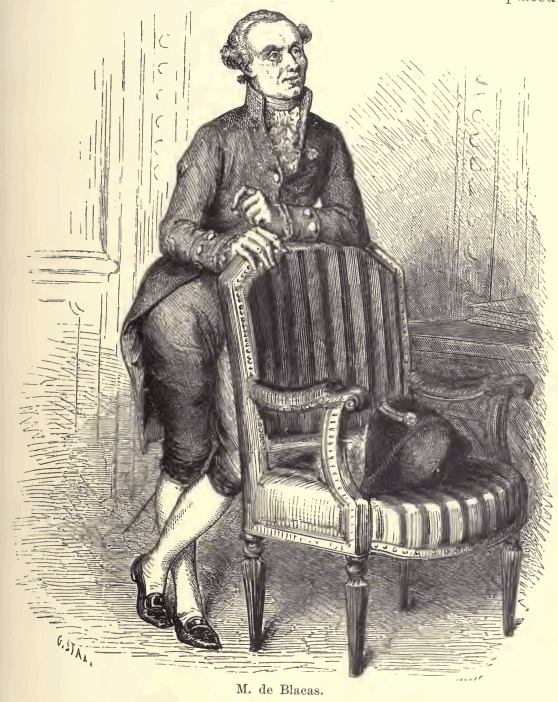
\includegraphics[width=\textwidth]{0141m.jpg}
\end{figure}

“So then,” he exclaimed, turning pale with anger, “seven conjoined and
allied armies overthrew that man. A miracle of heaven replaced me on
the throne of my fathers after five-and-twenty years of exile. I have,
during those five-and-twenty years, spared no pains to understand the
people of France and the interests which were confided to me; and now,
when I see the fruition of my wishes almost within reach, the power I
hold in my hands bursts and shatters me to atoms!”

“Sire, it is fatality!” murmured the minister, feeling that the
pressure of circumstances, however light a thing to destiny, was too
much for any human strength to endure.

“What our enemies say of us is then true. We have learnt nothing,
forgotten nothing! If I were betrayed as he was, I would console
myself; but to be in the midst of persons elevated by myself to places
of honor, who ought to watch over me more carefully than over
themselves,—for my fortune is theirs—before me they were nothing—after
me they will be nothing, and perish miserably from
incapacity—ineptitude! Oh, yes, sir, you are right—it is fatality!”

The minister quailed before this outburst of sarcasm. M. de Blacas
wiped the moisture from his brow. Villefort smiled within himself, for
he felt his increased importance.

“To fall,” continued King Louis, who at the first glance had sounded
the abyss on which the monarchy hung suspended,—“to fall, and learn of
that fall by telegraph! Oh, I would rather mount the scaffold of my
brother, Louis XVI., than thus descend the staircase at the Tuileries
driven away by ridicule. Ridicule, sir—why, you know not its power in
France, and yet you ought to know it!”

“Sire, sire,” murmured the minister, “for pity’s——”

“Approach, M. de Villefort,” resumed the king, addressing the young
man, who, motionless and breathless, was listening to a conversation on
which depended the destiny of a kingdom. “Approach, and tell monsieur
that it is possible to know beforehand all that he has not known.”

“Sire, it was really impossible to learn secrets which that man
concealed from all the world.”

“Really impossible! Yes—that is a great word, sir. Unfortunately, there
are great words, as there are great men; I have measured them. Really
impossible for a minister who has an office, agents, spies, and fifteen
hundred thousand francs for secret service money, to know what is going
on at sixty leagues from the coast of France! Well, then, see, here is
a gentleman who had none of these resources at his disposal—a
gentleman, only a simple magistrate, who learned more than you with all
your police, and who would have saved my crown, if, like you, he had
the power of directing a telegraph.” The look of the minister of police
was turned with concentrated spite on Villefort, who bent his head in
modest triumph.

“I do not mean that for you, Blacas,” continued Louis XVIII.; “for if
you have discovered nothing, at least you have had the good sense to
persevere in your suspicions. Any other than yourself would have
considered the disclosure of M. de Villefort insignificant, or else
dictated by venal ambition.” These words were an allusion to the
sentiments which the minister of police had uttered with so much
confidence an hour before.

Villefort understood the king’s intent. Any other person would,
perhaps, have been overcome by such an intoxicating draught of praise;
but he feared to make for himself a mortal enemy of the police
minister, although he saw that Dandré was irrevocably lost. In fact,
the minister, who, in the plenitude of his power, had been unable to
unearth Napoleon’s secret, might in despair at his own downfall
interrogate Dantès and so lay bare the motives of Villefort’s plot.
Realizing this, Villefort came to the rescue of the crest-fallen
minister, instead of aiding to crush him.

“Sire,” said Villefort, “the suddenness of this event must prove to
your majesty that the issue is in the hands of Providence; what your
majesty is pleased to attribute to me as profound perspicacity is
simply owing to chance, and I have profited by that chance, like a good
and devoted servant—that’s all. Do not attribute to me more than I
deserve, sire, that your majesty may never have occasion to recall the
first opinion you have been pleased to form of me.” The minister of
police thanked the young man by an eloquent look, and Villefort
understood that he had succeeded in his design; that is to say, that
without forfeiting the gratitude of the king, he had made a friend of
one on whom, in case of necessity, he might rely.

“’Tis well,” resumed the king. “And now, gentlemen,” he continued,
turning towards M. de Blacas and the minister of police, “I have no
further occasion for you, and you may retire; what now remains to do is
in the department of the minister of war.”

“Fortunately, sire,” said M. de Blacas, “we can rely on the army; your
majesty knows how every report confirms their loyalty and attachment.”

“Do not mention reports, duke, to me, for I know now what confidence to
place in them. Yet, speaking of reports, baron, what have you learned
with regard to the affair in the Rue Saint-Jacques?”

“The affair in the Rue Saint-Jacques!” exclaimed Villefort, unable to
repress an exclamation. Then, suddenly pausing, he added, “Your pardon,
sire, but my devotion to your majesty has made me forget, not the
respect I have, for that is too deeply engraved in my heart, but the
rules of etiquette.”

“Go on, go on, sir,” replied the king; “you have today earned the right
to make inquiries here.”

“Sire,” interposed the minister of police, “I came a moment ago to give
your majesty fresh information which I had obtained on this head, when
your majesty’s attention was attracted by the terrible event that has
occurred in the gulf, and now these facts will cease to interest your
majesty.”

“On the contrary, sir,—on the contrary,” said Louis XVIII., “this
affair seems to me to have a decided connection with that which
occupies our attention, and the death of General Quesnel will, perhaps,
put us on the direct track of a great internal conspiracy.” At the name
of General Quesnel, Villefort trembled.

“Everything points to the conclusion, sire,” said the minister of
police, “that death was not the result of suicide, as we first
believed, but of assassination. General Quesnel, it appears, had just
left a Bonapartist club when he disappeared. An unknown person had been
with him that morning, and made an appointment with him in the Rue
Saint-Jacques; unfortunately, the general’s valet, who was dressing his
hair at the moment when the stranger entered, heard the street
mentioned, but did not catch the number.” As the police minister
related this to the king, Villefort, who looked as if his very life
hung on the speaker’s lips, turned alternately red and pale. The king
looked towards him.

“Do you not think with me, M. de Villefort, that General Quesnel, whom
they believed attached to the usurper, but who was really entirely
devoted to me, has perished the victim of a Bonapartist ambush?”

“It is probable, sire,” replied Villefort. “But is this all that is
known?”

“They are on the track of the man who appointed the meeting with him.”

“On his track?” said Villefort.

“Yes, the servant has given his description. He is a man of from fifty
to fifty-two years of age, dark, with black eyes covered with shaggy
eyebrows, and a thick moustache. He was dressed in a blue frock-coat,
buttoned up to the chin, and wore at his button-hole the rosette of an
officer of the Legion of Honor. Yesterday a person exactly
corresponding with this description was followed, but he was lost sight
of at the corner of the Rue de la Jussienne and the Rue Coq-Héron.”
Villefort leaned on the back of an armchair, for as the minister of
police went on speaking he felt his legs bend under him; but when he
learned that the unknown had escaped the vigilance of the agent who
followed him, he breathed again.

“Continue to seek for this man, sir,” said the king to the minister of
police; “for if, as I am all but convinced, General Quesnel, who would
have been so useful to us at this moment, has been murdered, his
assassins, Bonapartists or not, shall be cruelly punished.” It required
all Villefort’s coolness not to betray the terror with which this
declaration of the king inspired him.

“How strange,” continued the king, with some asperity; “the police
think that they have disposed of the whole matter when they say, ‘A
murder has been committed,’ and especially so when they can add, ‘And
we are on the track of the guilty persons.’”

“Sire, your majesty will, I trust, be amply satisfied on this point at
least.”

“We shall see. I will no longer detain you, M. de Villefort, for you
must be fatigued after so long a journey; go and rest. Of course you
stopped at your father’s?” A feeling of faintness came over Villefort.

\begin{figure}[h]
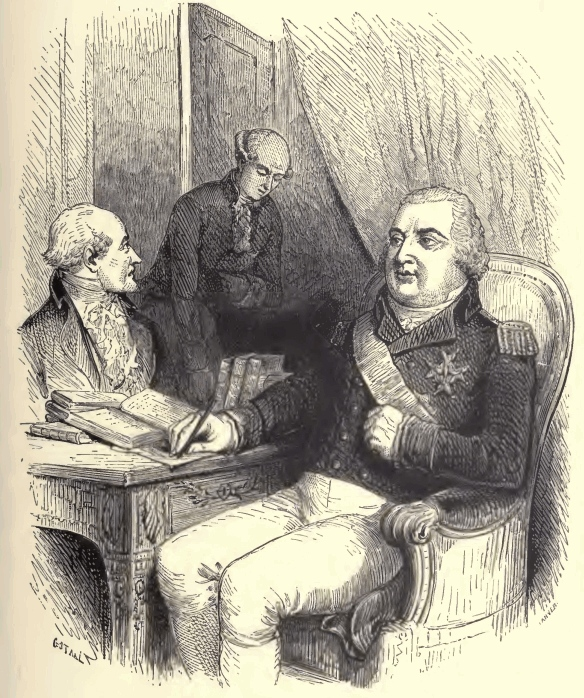
\includegraphics[width=\textwidth]{0145m.jpg}
\end{figure}

“No, sire,” he replied, “I alighted at the Hotel de Madrid, in the Rue
de Tournon.”

“But you have seen him?”

“Sire, I went straight to the Duc de Blacas.”

“But you will see him, then?”

“I think not, sire.”

“Ah, I forgot,” said Louis, smiling in a manner which proved that all
these questions were not made without a motive; “I forgot you and M.
Noirtier are not on the best terms possible, and that is another
sacrifice made to the royal cause, and for which you should be
recompensed.”

“Sire, the kindness your majesty deigns to evince towards me is a
recompense which so far surpasses my utmost ambition that I have
nothing more to ask for.”

“Never mind, sir, we will not forget you; make your mind easy. In the
meanwhile” (the king here detached the cross of the Legion of Honor
which he usually wore over his blue coat, near the cross of St. Louis,
above the order of Notre-Dame-du-Mont-Carmel and St. Lazare, and gave
it to Villefort)—“in the meanwhile take this cross.”

“Sire,” said Villefort, “your majesty mistakes; this is an officer’s
cross.”

“\textit{Ma foi!}” said Louis XVIII., “take it, such as it is, for I have not
the time to procure you another. Blacas, let it be your care to see
that the brevet is made out and sent to M. de Villefort.” Villefort’s
eyes were filled with tears of joy and pride; he took the cross and
kissed it.

“And now,” he said, “may I inquire what are the orders with which your
majesty deigns to honor me?”

“Take what rest you require, and remember that if you are not able to
serve me here in Paris, you may be of the greatest service to me at
Marseilles.”

“Sire,” replied Villefort, bowing, “in an hour I shall have quitted
Paris.”

“Go, sir,” said the king; “and should I forget you (kings’ memories are
short), do not be afraid to bring yourself to my recollection. Baron,
send for the minister of war. Blacas, remain.”

“Ah, sir,” said the minister of police to Villefort, as they left the
Tuileries, “you entered by luck’s door—your fortune is made.”

“Will it be long first?” muttered Villefort, saluting the minister,
whose career was ended, and looking about him for a hackney-coach. One
passed at the moment, which he hailed; he gave his address to the
driver, and springing in, threw himself on the seat, and gave loose to
dreams of ambition.

Ten minutes afterwards Villefort reached his hotel, ordered horses to
be ready in two hours, and asked to have his breakfast brought to him.
He was about to begin his repast when the sound of the bell rang sharp
and loud. The valet opened the door, and Villefort heard someone speak
his name.

\begin{figure}[h]
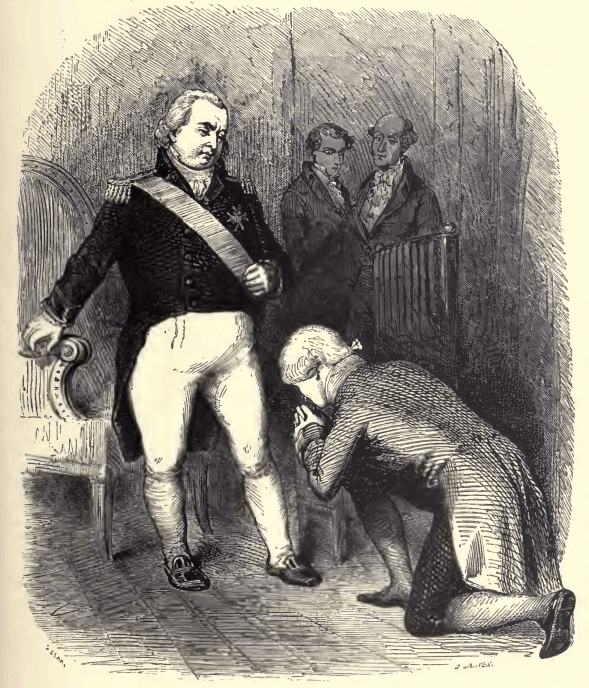
\includegraphics[width=\textwidth]{0147m.jpg}
\end{figure}

“Who could know that I was here already?” said the young man. The valet
entered.

“Well,” said Villefort, “what is it?—Who rang?—Who asked for me?”

“A stranger who will not send in his name.”

“A stranger who will not send in his name! What can he want with me?”

“He wishes to speak to you.”

“To me?”

“Yes.”

“Did he mention my name?”

“Yes.”

“What sort of person is he?”

“Why, sir, a man of about fifty.”

“Short or tall?”

“About your own height, sir.”

“Dark or fair?”

“Dark,—very dark; with black eyes, black hair, black eyebrows.”

“And how dressed?” asked Villefort quickly.

“In a blue frock-coat, buttoned up close, decorated with the Legion of
Honor.”

“It is he!” said Villefort, turning pale.

\begin{figure}[h]
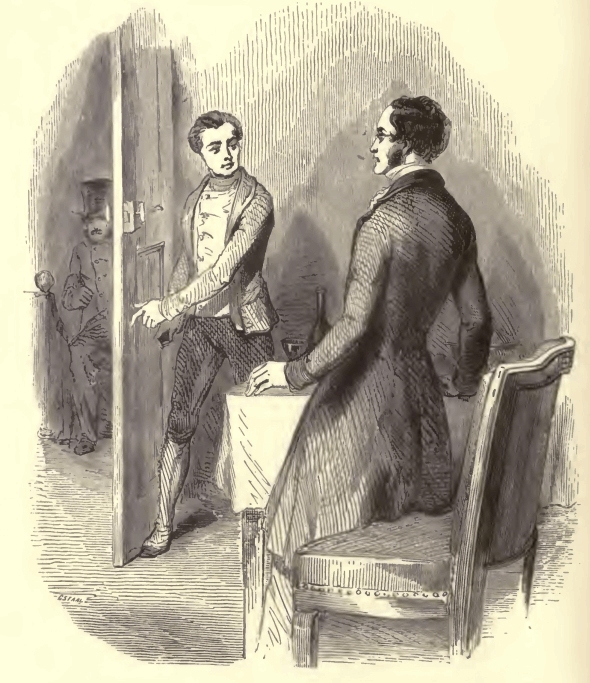
\includegraphics[width=\textwidth]{0148m.jpg}
\end{figure}

“Eh, \textit{pardieu!}” said the individual whose description we have twice
given, entering the door, “what a great deal of ceremony! Is it the
custom in Marseilles for sons to keep their fathers waiting in their
anterooms?”

“Father!” cried Villefort, “then I was not deceived; I felt sure it
must be you.”

“Well, then, if you felt so sure,” replied the new-comer, putting his
cane in a corner and his hat on a chair, “allow me to say, my dear
Gérard, that it was not very filial of you to keep me waiting at the
door.”

“Leave us, Germain,” said Villefort. The servant quitted the apartment
with evident signs of astonishment.

\chapter{MAN THE OFFSPRING OF GOD}

THE contaminating influence of organic evolution has found its way into every branch of
education. Naturally history cannot escape because history has to deal with man and his
civilization. Historical facts, however, cannot go back of written records, therefore it is
customary for scientists to deal with ancient peoples through the study of geology, biology,
anthropology and archaeology. These studies are young and full of surmises and guesses, and
thus are based on many uncertain deductions. The first great error made by these researchers
is in relation to the age of the earth. Evolution demands great periods of time for its purpose,
and the advocates in the imagination of their hearts have chosen a time far beyond the
knowledge and the power of research to fathom. Sociology has followed in their footsteps
and these studies cannot, and rightfully should not, be considered authentic. There are many
who have accepted these theoretical conclusions and thus we find the blind leading the blind
and all have fallen into the ditch. It is not the purpose here to consider the age of the earth, or
to enter into a discussion of this so-called scientific research. At this point it is sufficient to
discuss the origin of man from the scriptural point of view. It is nevertheless necessary to
refer to these theories in relation to early man for they have been published in nearly every
historical textbook on ancient history since the middle of the nineteenth century. At the
present day in the public schools ancient history begins with "prehistoric man," and places
him many thousands of years before there were any written records. The "primitive man"
according to these texts was a savage without culture, crude in his appearance, and
worshiping his shadow, the sun, moon, stars, the forces of nature, animals that awed him and
objects or forces which he did not understand. According to the theory he became an idol
worshiper when he had advanced enough in experience to carve himself gods of wood or
stone. Thus he was polytheistic in his worship. Much of this nonsense has been refuted by
better research.

W. Schmidt, professor in the University of Vienna, an expert in his field on Comparative
Religions, in his book, \textit{The Origin and Growth of Religion—Facts and Theories}, maintains
that the farther we go back in time the more it is discovered that the "primitive" nations were
monotheistic in their worship. In this book, translated by H. J. Rose, we find the following in
Chapter XVI on \textit{The Primitive High God:}

That the Supreme Being of the primitive culture is really the god of a monotheism, and the
religion which includes him is genuinely monotheistic—this is the position which is most
attacked by a number of authors. To this attack we may reply that there is a sufficient number
of tribes among whom the really monotheistic character of their Supreme Being is clear even
to a cursory examination. This is true of the Supreme Being of most Pygmy tribes, so far as
we know them; also of the Tierra del Fuegians, the primitive Bushmen, the Kurnai, Kulin and
Yuin of South-East Australia, the peoples of the Arctic culture, except the Koryaks, and well-
nigh all of the primitives of North America.

Among other races, the fact of their monotheistic belief has been obscured. This is partly due
to crosses with later forms, partly to differentiation, partly to other causes, all of which can
be discovered only by exact historical analysis. (Page 262.)

In nearly every separate area of the primitive culture the First Father plays an important part,
especially in the initiation ceremonies; originally he and the First Mother were the parents of
the race. Owing to the latter influence of the matrilineal cultures, he develops a lunar
character, is brought into connection with the moon and not uncommonly obscures the
Supreme Being or blends with him. . . . The Supreme Being is everywhere represented
among them as absolutely good, having nothing to do with evil either in conduct or in the
outer world. Evil therefore must have another vehicle or originator; and he, especially in the
mythology of the North American primitives and of those of the Arctic, is opposed to the
Supreme Being; his origin, however, remains darkly mysterious. . . . (Page 263.)

This leads us to a whole series of other races, among whom the Supreme Being is described
as "shining white" "or like fire"; for example, among the North-Western Semang, the
Southern Andamanese, the Wiyot and Patwin of North Central California, the Lenape, an
Algonquin tribe, and the Winnebago, a Sioux tribe influenced by the Algonquin. Among the
Maidu of North Central California we are assured that the whole form of the Supreme Being
shines like the light of the sun, but that his face is always covered and no one has ever seen it,
except the Evil Spirit, who did so once. The Kurnai and Wiradyuri teach that the Supreme
Being is surrounded by an aureole of sunrays. Among the Samoyeds a shaman saw him
blazing with so bright a light that he could not look at him. . . .

The name "father" is applied to the Supreme Being in every single area of the primitive
culture when he is addressed or appealed to. It seems, therefore, that we may consider it
primeval and proper to the oldest primitive culture. We find it in the form "father" simply,
also in the individual form ("my father") and the collective ("our father"). So far, this name
has not been discovered among the Central African Pygmies, but it exists among the
Bushmen and the Mountain Dama. It is lacking also among the Andamanese and the
Philippine Negritos, but is found, although not commonly, among the Semang. Among the
Samoyeds we find the formula, "My Num-father," i.e. sky-father. In North Central
California, the name occurs among the Pomo and the Patwin; all three forms of it are widely
distributed among the Algonquins. It is also widely current among the two oldest Tierra del
Fuegian tribes, the Yamana and the Halakwulup who use the form "my father." Among all
the tribes of Southeast Australia it is in common use, in the form "our father." There it is the
oldest name of all, and even the women and children know it; the oldest of the tribes, the
Kurani, have no other name for him. There is no doubt possible that the name "father" is
intended in this connection to denote, not physiological paternity (save in cases where the
figures of the Supreme Being and the First Father have coalesced), but an attitude of the
greatest reverence, of tender affection and steadfast trust on the part of man towards God.
(Pages 266-268.)

From all of this it would appear that the knowledge of God had been handed down by
tradition from the days of Adam and Noah. For the antediluvians knew him as shining like
the sun, and the Israelites were frightened when they were given the invitation to meet him in
the Mount." (Exodus 19:9-22; 33:9, 10, 11, 21, 22, 23.)

To show this modern trend here are two illustrations:

The first step towards civilization must have been uncertain and slow. No doubt these
beginnings took long periods of time, but we can know little about them, for no people leaves
records that the historian can use until it has advanced a long way from primitive savagery.

To be sure, there are tribes still in primitive stages; and, by comparing them with what can be
gleaned from traditions, customs, words, and early records of our civilization, scholars have
learned something of how our fore-fathers must have lived before Homer and before the
oldest inscriptions upon Egyptian stone. . . .

Still it is well for us to remember that our imposing and varied civilization rests upon this
unrecorded work of prehistoric man through slow, uncounted ages. The development of
language, the invention of the bow, of making fire, of pottery to stand the fire; the
domestication of the dog and cow; the learning to live together, not in droves, but in families
and tribes; the rude beginnings of agriculture; the smelting of metals to replace stone tools;—
these are steps any of which are infinitely more important than the discovery of electricity or
the growth of federal government: but all this, and much more, had become the common
property of many races before history began anywhere. 1

It has taken thousands of years for man to develop from his early state of savagery and
helplessness to the condition in which we now live. In order to understand thoroughly our
present life, it is necessary to study the slow growth of mankind through these past ages. This
story or record of the past life and development of man is the science called history. That part
of the story which is commonly called "Ancient History" covers over 4,000 years, extending
from the time when first we know of men through reliable records, down to about 800 years
after the birth of Christ. . . .

The prehistoric ages of man's development stretch back for unknown thousands of years.
During this time, man was slowly learning by bitter experience to light fires, to cook food,
and to tame and make use of some of the gentler animals, such as the dog and the horse.
Then came the knowledge of the value of certain kinds of grain, and the raising of crops.
This long space of time has been divided by historians into four periods, according to the
material used in making hatchets, knives, spearheads, and arrow heads.

1. The Paleolithic or Rough Stone Age.

2. The Neolithic or Polished Stone Age.

3. The Bronze Age.

4. The Iron Age.

The change from savage or barbarous ways of living to what we call "civilized" life, did not
take place at one time in all parts of the earth. Some tribes of the Philippine Islands, of
Australia, Africa, and South America are still using tools made of bone and stone. Even now
they are in the state of savagery characteristic of the Stone Age. Yet, at least 6,000 years ago,
the Egyptians were a cultured people, far advanced in the civilization of the Bronze Age and
to a limited extent they even used iron tools. 2

It is the purpose of this chapter to show that these conclusions are incorrectly based and are
founded in imagination and speculation, influenced by the evolutionary theory. If they be
true then the Bible is fiction. If they be true, the Lord never revealed himself to ancient man.
If so, the story of Adam and Eve falls to the ground as a fable. If there was no "Fall"
consequently there could be no Atonement, for if there had been no Fall there had been no
need of Jesus Christ who came into the world to be its Redeemer from a fallen state, and give
back to mankind that which had been taken away by Adam's transgression. There is no
middle ground! If these writers of history and these teachers of man's gradual progress from
animal forms were correct—and that is definitely implied in all of these so-called historical
conclusions in relation to "savage primitive man"—then the Christian faith would be false.
On the other hand if Christ is true; if he came into the world as he proclaimed himself, to
restore man to life that he might have it more abundantly, and he is verily "The Resurrection
and the Life," then all of this twaddle and speculation is trash! By overwhelming evidence it
is my duty to show that this modernistic teaching is false and that God is true and his
Beloved Son Jesus Christ accomplished his mission as the Savior of men and Redeemer of
the world!

I write to members of the Church of Jesus Christ of Latter-day Saints. You have a right to
know the truth, to be endowed with an abiding testimony. You have the right to know that
God lives and that Jesus Christ is his Only Begotten Son in the flesh, who came into the
world, preordained to be a sacrifice for a fallen world and give to all those who repent and
obey his commandments eternal life. This truth you have the means of knowing, for the
promise has been made to you that—

If ye continue in my word, then are ye my disciples indeed;

And ye shall know the truth, and the truth shall make you free. 3

Also it is written:

My doctrine is not mine, but his that sent me.

If any man will do his will, he shall know of the doctrine, whether it be of God, or whether I
speak of myself. 4

I assure you that this promise never fails the sincere, humble searcher after truth.

These advocates of evolution say there are four ages of man: 1. The Paleolithic; 2. The
Neolithic; 3. The Bronze Age; 4. The Age of Iron, but these have little meaning in the Gospel
of Jesus Christ, as representing four stages of man from the lowly savage to the cultured man
of our day. All of this is in contradiction of the revelations of God to man. No doubt the first
man on the earth had to learn by experience, line upon line and precept upon precept, but he
was not left to grope in darkness from the use of a bone weapon or a stick with which to
plow. Nor was he under the necessity of finding out the hard way that there were grains and
vegetables, and flocks at his disposal. To cultivate the soil he was commanded; but he had a
heavenly instructor and by revelation many things for his advancement were made known to
him and to his children. One of the first lessons that he learned, by divine instruction, was to
clothe his naked body. He was commanded to till the soil. When sons were born to him they
followed the course of the father. The first man was not a savage, but a gentle god-fearing
man, full of faith and understanding the Gospel for he was taught by our Eternal Father, and
angels sent from his presence. He was commanded to eat the herb of the field, to cultivate it
by the industry of his hands, and the sweat of his face, and prepare the grain to make his
bread. Domestic animals were placed at his command. One of the first sons born to him was
a "keeper of sheep" that clothing might be provided, not skins. The other was a tiller of the
soil and raised "the fruit of the ground." They were not idle roaming men, but builders of
communities. They did not have to learn to domesticate "the dog and cow."

These authors delight in referring to the fact that there are "primitive" people on the face of
the earth today, but their ancestors were not "primitive" in the sense in which this word is
used, nor were they in "savagery." The ancient ancestors of the African savage now in the
"stone age," in the third generation from the first man, were musicians and made harps and
organs, and were artificers in brass and iron. 5 And mark you, this was in the morning of
man's presence on the earth. Then be it remembered that the ancestors of the savage South
American were men of superior intelligence who loved the Lord and kept his
commandments. They were a very enlightened people. They had prophets among them and
received revelation from the Lord to guide them. It was due to rebellion against the light of
truth and turning from righteousness to wickedness that brought these South Americans to
the pitiful plight in which they now find themselves. They were not polytheistic and
worshipers who had to manufacture their religion and create their gods. The Eternal Father of
us all gave them commandments and revealed to them the plan of salvation and taught them
of the coming of the Son of God, even Jesus Christ, to redeem them from their fallen state.
The knowledge of God was known by the first man placed on this earth. At one time he
dwelt in the presence of God; was taught by him, learned his language and taught his
children to worship the Father in the name of Jesus Christ his Son. The first man and his sons
and daughters were not forced to develop a language, to make fires and come up through
"thousands of years" from a state of savagery and helplessness, to the condition in which we
now live." The Lord has revealed to us much of the history of the first man and his
descendants. It is recorded in the revelations of the Lord that after Adam, the first man, had
been driven from the Garden to till the ground he was commanded to worship the Father and
offer sacrifice to him.

And he gave unto them commandments, that they should worship the Lord their God, and
should offer the firstlings of their flocks, for an offering unto the Lord. And Adam was
obedient unto the commandments of the Lord.

And after many days an angel of the Lord appeared unto Adam, saying: Why dost thou offer
sacrifices unto the Lord? And Adam said unto him: I know not, save the Lord commanded
me.

And then the angel spake, saying: This thing is a similitude of the sacrifice of the Only
Begotten of the Father, which is full of grace and truth.

Wherefore, thou shalt do all that thou doest in the name of the Son, and thou shalt repent and
call upon God in the name of the Son forevermore. 6

The knowledge of God was known among the first inhabitants of this earth. Furthermore,
they were not left to struggle without divine aid in matters of language for it has been also
revealed that Adam and his immediate posterity were taught in the language of God.

And God revealed himself unto Seth, and he rebelled not, but offered an acceptable sacrifice,
like unto his brother Abel. And to him also was born a son, and he called his name Enos.

And then began these men to call upon the name of the Lord, and the Lord blessed them;

And a book of remembrance was kept, in the which was recorded, in the language of Adam,
for it was given unto as many as called upon God to write by the spirit of inspiration;

And by them their children were taught to read and write, having a language which was pure
and undefiled.

Now this same Priesthood, which was in the beginning, shall be in the end of the world also.

Now this prophecy Adam spake, as he was moved upon by the Holy Ghost, and a genealogy
was kept of the children of God. And this was the book of the generations of Adam, saying:
In the day that God created man, in the likeness of God made he him;

In the image of his own body, male and female, created he them, and blessed them, and
called their name Adam, in the day when they were created and became living souls in the
land upon the footstool of God. 7

Here we are informed that man was created in the image of God. This is repeated several
times in the Book of Genesis in speaking of the creation of man. 8 This is the answer to the
evolutionist in relation to the descent of man, and to all religionists as well as scientists who
ridicule the anthropomorphic nature of God. Man was created in the likeness of the body of
God. We call him Father, we are taught that he is literally the Father of the spirits of all men,
and in the spirit they were created, or begotten, sons and daughters unto him. 9 Paul declared
that we are his offspring and that he has "made of one blood all nations of men for to dwell
on all the face of the earth, and hath determined the times before appointed, and the bounds
of their habitation." 10

Members of the Church of Jesus Christ of Latter-day Saints are under obligation to accept the
Bible as the word of God as far as it is translated correctly. We know that there are many
errors in the translations current among the nations. There are many places where different
interpretations are placed upon important passages thus causing confusion and the teaching
of false doctrine. Nevertheless in regard to the relationship of man to God in practically all of
these translations there is agreement. God is our Father. Adam and Eve were created in his
image. Modern revelation, the scriptures which have been restored in the Book of Mormon,
the Book of Moses, of Abraham, the Doctrine and Covenants, all bear witness that man is the
offspring of God, and that man was created in his image. Therefore there is a challenge to all
these theories of men who teach the descent of man through countless ages from lower forms
of life. The revelations of the Lord being true, these theories are false.

We discover in the revelations that man was intelligent in the beginning. It is made known
that Adam is none other than Michael, the Arch-angel, who was sent to this earth to stand at
the head and be a prince over his posterity forever. 11 It was revealed to the Prophet Joseph
Smith that Methuselah was acquainted with the heavenly bodies, and that he had it revealed
unto him that Kolob is the first grand governing star and this was made known to the fathers.
Moreover, it was revealed that the records of the fathers before the flood were handed down
from generation to generation so that mankind could have knowledge of the dealings of God
with the fathers before the flood. These records fell into the hands of Abraham who wrote
about them as follows:

But the records of the fathers, even the patriarchs, concerning the right of Priesthood, the
Lord my God preserved in mine own hands; therefore a knowledge of the beginning of the
creation, and also of the planets, and of the stars, as they were made known unto the fathers,
have I kept even unto this day, and I shall endeavor to write some of these things upon this
record, for the benefit of my posterity that shall come after me. 12

So we learn from this and from many other sources, that the art of writing and the keeping of
records and knowledge of astronomy are very old. In fact this knowledge has come down
from the beginning, even from Adam who was taught to read and write in a perfect language,
for it was the language of God. We are informed that Enoch wrote a record, the history of the
earth and its inhabitants from the beginning down to the end of time. This was done by vision
and revelation, for the Lord opened to his mind and "showed Enoch all things, even unto the
end of the world; and he saw the day of the righteous, the hour of their redemption; and
received a fulness of joy." 13 Moses also was blessed with a similar view and this is
recorded:

And calling upon the name of God, he beheld his glory again, for it was upon him; and he
heard a voice, saying: Blessed art thou, Moses, for I, the Almighty, have chosen thee, and
thou shalt be made stronger than many waters; for they shall obey thy command as if thou
wert God.

And lo, I am with thee, even unto the end of thy days; for thou shalt deliver my people from
bondage, even Israel my chosen.

And it came to pass, as the voice was still speaking, Moses cast his eyes and beheld the earth,
yea, even all of it; and there was not a particle of it which he did not behold, discerning it by
the Spirit of God.

And he beheld also the inhabitants thereof, and there was not a soul which he beheld not; and
he discerned them by the Spirit of God; and their numbers were great, even numberless as the
sand upon the sea shore.

And he beheld many lands; and each land was called earth, and there were inhabitants on the
face thereof.

And it came to pass that Moses called upon God, saying: Tell me, I pray thee, why these
things are so, and by what thou madest them?

And behold, the glory of the Lord was upon Moses, so that Moses stood in the presence of
God, and talked with him face to face. And the Lord God said unto Moses: For mine own
purpose have I made these things. Here is wisdom and it remaineth in me.

And by the word of my power, have I created them, which is mine Only Begotten Son, who
is full of grace and truth.

And worlds without number have I created; and I also created them for mine own purpose;
and by the Son I created them, which is mine Only Begotten.

\textit{And the first man of all men have I called Adam, which is many}

But only an account of this earth, and the inhabitants thereof, give I unto you. For behold,
there are many worlds that have passed away by the word of my power. And there are many
that now stand, and innumerable are they unto man; but all things are numbered unto me, for
they are mine and I know them.

And it came to pass that Moses spake unto the Lord, saying: Be merciful unto thy servant, O
God, and tell me concerning this earth, and the inhabitants thereof, and also the heavens, and
then thy servant will be content.

And the Lord God spake unto Moses, saying: The heavens, they are many, and they cannot
be numbered unto man; but they are numbered unto me, for they are mine.

\textit{And as one earth shall pass away, and the heavens thereof even so shall another come; and
there is no end to my works neither to my words.}

\textit{For behold, this is my work and my glory—to bring to pass the immortality and eternal life of
man.} 14

Here we have the Lord's reason for the building of earths and the peopling of them with the
sons and daughters of God. Moses was favored with a vision in which he saw all of the earth
and its inhabitants. Afterwards the Lord explained to him how his works are carried on and to
which there is no end. The first man on the earth was named Adam, because he was to be the
father of many. This earth on which we stand is only one of many earths, numberless unto
man, but numbered and known unto God. We also learn that earths are formed as habitations
for his offspring, his sons and daughters. His great work and glory being to people these
earths and grant unto his offspring the blessings of immortality or eternal life. In order to
obtain immortality, the spirit and the body must be inseparably connected, the children of
God must pass through a probation such as we are passing through on this earth. They must
have a season of mortality and become familiar with all the vicissitudes of a temporal
probation. Mortal life is a probationary state 15 where we are to be tried, proved, as gold is
tried in the crucible, to see if we will keep all of the commandments of God. If we pass
through this probation successfully we will be entitled to eternal life, if we fail we will be
given immortality. Eternal life is to have the same kind of life, with its glory, that God
possesses; immortality is to have the blessing of living forever, after the resurrection of the
dead, but not with the same glory and blessings which are held in store for those who are just
and true. We learn from these teachings given to Moses that Man is the greatest of all the
creations—for he is the offspring of God. Worlds, or earths, are built as habitations for man
and they too pass through a temporal probationary state corresponding to that of man. Some
earths that have been built and some that are now being created are for habitations for those
who receive immortality; others are to become celestial earths and the eternal abodes of those
who become members of the "Church of the Firstborn," in other words, are true and faithful
to every commandment, covenant and obligation required for exaltation in the Gospel of
Jesus Christ. The Lord in his mercy provides eternal earths for all mankind, each individual
going to his own place according to his works.

The doctrine taught by science, especially by astronomers, is that we live in a changing
universe, that the heavenly bodies had a beginning in which great heat was generated, but
that they are cooling and eventually will become dead cold bodies traveling their uncertain
courses eternally, unless in eons of ages they disintegrate to be made over again. Some
members of the Church, in reading the words of the Lord to Moses have interpreted these
words: "And as one earth shall pass away, and the heavens thereof even so shall another
come" with this same understanding. This, however, is not the meaning of the Lord. He does
not create anything to be destroyed. He has said that at no time has he given unto men "a law
which was temporal; neither any man, nor the children of men; neither Adam, your father,
whom I created." 16 The key to this statement is given to the Church in relation to the destiny
of this earth, in the Doctrine and Covenants (88:15-20, 25-26.)

And the spirit and the body are the soul of man.

And the resurrection from the dead is the redemption of the soul.

And the redemption of the soul is through him that quickeneth all things, in whose bosom it
is decreed that the poor and the meek of the earth shall inherit it. [i.e. the earth when
celestialized.]

Therefore, it must needs be sanctified from all unrighteousness, that it may be prepared for
the celestial glory;

For after it hath filled the measure of its creation, it shall be crowned with glory, even with
the presence of God the Father;

That bodies who are of the celestial kingdom may possess it forever and ever; for, for this
intent was it made and created, and for this intent are they sanctified. . .

And again, verily I say unto you, the earth abideth the law of a celestial kingdom, for it filleth
the measure of its creation, and transgresseth not the law—

Wherefore, it shall be sanctified; yea, notwithstanding it shall die, it shall be quickened again,
and shall abide the power by which it is quickened, and the righteous shall inherit it.

We read in the Bible where the prophets speak of this passing away, first we quote Peter who
declares this will come:

The Lord is not slack concerning his promise, as some men count slackness; but is
longsuffering to us-ward, not willing that any should perish, but that all should come to
repentance.

This from Isaiah:

Lift up your eyes to the heavens, and look upon the earth beneath: for the heavens shall
vanish away like smoke, and the earth shall wax old like a garment, and they that dwell
therein shall die in like manner: but my salvation shall be for ever, and my righteousness
shall not be abolished. 17

From the Psalms:

Of old hast thou laid the foundation of the earth: and the heavens are the work of thy hands.

They shall perish, but thou shalt endure: yea, all of them shall wax old like a garment; as a
vesture shalt thou change them, and they shall be changed. 18

Our Lord himself said:

Heaven and earth shall pass away, but my words shall not pass away. 19

The passing away of the heavens has reference to the heavens which surround the earth, not
the sidereal heavens. So we have a key to the meaning of one earth passing away and another
coming. As our earth shall pass away and receive its resurrection, so has it been with other
earths and so will it be with earths yet to come. They will be re-created, made eternal and
find a place perpetually which the Lord has designed for them in the sidereal heavens. These
great orbs that we see in the heavens are not "passing away." Most of them evidently have
attained their state of permanency. They have filled the measure of temporal probation as this
earth is now filling its probation of mortality, and when its work is finished as a temporal
earth it will be exalted. Likewise will others be exalted as countless earths have been and
have attained their state of immortality.

I suppose this is one of the lowest kingdoms that ever the Lord Almighty created, and on that
account is capable of becoming exalted to be one of the highest kingdoms that has ever had
an exaltation in all the eternities. In proportion as it has been reduced so it will be exalted,
with that portion of its inhabitants who in their humiliation have cleaved to righteousness and
acknowledged God in all things.—President Brigham Young, \textit{J. of D.}, 10:175.

This is the testimony of Elder Orson Pratt:

But there is another thing to be considered. Are the wicked to receive this earth as an
inheritance? No; for Jesus did not say, Blessed are the wicked, for they shall inherit the earth;
this promise was made only to the meek. Who are the meek: None but those who receive the
same ordinances the earth has received, and be baptized with fire and with the Holy Ghost, as
this earth will be when Jesus comes to reign upon it a thousand years; and be clothed upon
with the glory of God, as the earth will be; and after they have died as the earth will die, they
will have to be resurrected, as this earth will be resurrected, and then receive their inheritance
upon it.—Orson Pratt, \textit{J. of D.} 1:293.

This from President Charles W. Penrose:

The destiny of this globe is to be fitted as a habitation for the righteous and "meek" of the
earth, who will inherit it in their resurrected state. The Lord has revealed that "the earth
abideth the law of its creation," and when it has fully filled the measure thereof, it shall be
crowned with glory, "even with the presence of the Father;" that "although it shall die, it shall
be quickened again" and shall be inhabited by beings clothed with the celestial glory; that
"for this intent was it made and created." (See D. \& C. 88:17-26.) There are many other
particulars concerning the future of this planet, formed by the Eternal as a dwelling place for
this branch of the great family of which he is the head, but on these we will not discourse
further at present.—President Charles W. Penrose, \textit{Liahona}, 6:999.

We now come to this vital point. My fellow believers in the mission of Jesus Christ, in
Joseph Smith and the restoration of the Gospel, as I have said, you are entitled through
faithfully keeping the commandments of the Lord, to individual guidance. It is your right
under these conditions to \textit{know the truth} which makes us free. You cannot be a true member
of the Church and reject Jesus Christ. You cannot be a faithful member and reject the
scriptures—Bible, Book of Mormon, Doctrine and Covenants and Pearl of Great Price—for
these are the standards of our faith. If you accept them you \textit{cannot} accept organic evolution,
for they are diametrically opposed. We will have more to consider in relation to man, his
origin and destiny, in chapters yet to come. Now let us reason together on what is here
presented:

1. Worlds without number have been created.

2. They have been created as habitations for the children of God.

3. The great work and glory of our Father is to bring to pass the immortality and eternal life
of man.

4. Inhabitants of other worlds are begotten sons and daughters of God.

5. When one earth passes away to its exaltation another comes.

6. The making of earths is a glorious work which has been carried on eternally.

This being true, then does it not appear to you that it is a foolish and ridiculous notion that
when God created this earth he had to begin with a speck of protoplasm, and take millions of
years, if not billions, to bring conditions to pass by which his sons and daughters might
obtain bodies made in his image? Why not the shorter route and \textit{transplant} them from
another earth as we are taught in the scriptures? Surely to any reasonable mind, the Lord
would not have to start with an amoeba, pass through the stage of lower fish to higher fish to
reptiles to apes and to man! When we stop to consider how perfect are the workings of God;
how thorough he is and orderly, surely these theories flatten out and are without substance.
Then we have this to think about. According to the revelations to Moses and Abraham, as
given to us in the Pearl of Great Price in clearness, and also stated in the Bible, does it not
seem rather out of harmony for a Latter-day Saint to believe that several billion years ago,
according to our reckoning, there was a council held in heaven at which we shouted for joy
because we were to have the opportunity of coming to the earth to receive bodies that we
might become, through faithfulness, like unto our Father, God? At that time many of the
great and noble spirits were chosen to become rulers. According to the theories of men, if we
believe the revelation of that pre-existence, we had to wait, some say several billions of
years, before that promise could be accomplished.

Also be it remembered, and all who accept the Gospel should remember it, every creature is
eternal. Evolutionists do not believe in the existence of spirit, for man or animal, but we, as
members of the Church do. The Lord has revealed it:

2. Q. What are we to understand by the four beasts, spoken of in the same verse [i. e.
Revelation 4:6.]

\textit{A. They are figurative expressions, used by the Revelator, John, in describing heaven, the
paradise of God, the happiness of man, and of beasts, and of creeping things, and of the
fowls of the air; that which is spiritual being in the likeness of that which is temporal; and
that which is temporal in the likeness of that which is spiritual; the spirit of man in the
likeness of his person, as also the spirit of the beast, and every other creature which God has
created.} (D. \& C. 77:2.)

Here we are informed that God created the beasts as well as man, creeping things, the fowls
of the air and placed in each a spirit in the exact likeness of its body, or more properly,
created every creature in the likeness of its spirit. Therefore they are living entities entitled to
the mercies of Jesus Christ and to receive the resurrection. Then again, the Lord revealed that
every creature shall receive a resurrection:

And again, verily, verily, I say unto you that when the thousand years are ended
[Millennium,] and men again begin to deny their God, then will I spare the earth but for a
little season;

And the end shall come, and the heaven and the earth shall be consumed and pass away, and
there shall be a new heaven and a new earth.

For all old things shall pass away, and all things shall become new, even the heaven and the
earth, and all the fulness thereof, both men and beasts, the fowls of the air, and the fishes of
the sea;

\textit{And not one hair, neither mote, shall be lost, for it is the workmanship of mine hand.} 20

So we learn that all things were created by our Eternal Father, and there is nothing which has
life that he did not create; moreover \textit{every thing shall live again receiving the benefit of the
resurrection.} This proves that \textit{every thing having life}, is endowed with a spirit, and \textit{had a fall.}
In other words became mortal following the transgression of Adam. This also applies to the
earth itself. It was not created a mortal, or temporal earth, but this was acquired when the
curse was placed upon it after Adam's transgression. We have previously referred to the word
of the Lord that—

Wherefore, verily I say unto you that all things unto me are spiritual, and not at any time
have I given unto you a law which was temporal; neither any man, nor the children of men;
neither Adam, your father, whom I created. (D. \& C. 29:34.)

Here again we find the Gospel—the revelations from the Lord—in conflict with geological
and evolutionary teachings. If there were creatures on the earth before Adam, especially men,
where did they obtain their mortal life? They could not be created mortal (temporal) by our
Eternal Father, for that would contradict his own word. If they were created first spiritual and
partook of a fall, who brought that fall upon them? If they were originally made mortal and
subject to death, then they were not entitled to a redemption from death, and since the Lord is
not the author of death, how did they obtain it? Further, how are they entitled to a redemption
and restoration to something that they never had? The whole thing is absurd. All life comes
from God and he did not create it temporally, that was achieved through the violation of a
law. There is no Redeemer other than Jesus Christ for this earth and since Adam could not
have brought death on pre-Adamite life, such life could not obtain the blessings of the
resurrection. Yet the Lord has declared that through the atonement all things partaking of the
fall will be redeemed. So there were no pre-Adamites.

Another thing I wish to say. A man cannot serve God and mammon. Organic evolution is
destructive of faith in God. It is rebellion against him. Those who accept this pernicious
doctrine cannot consistently believe in the fall of Adam. If they do not believe in the fall of
Adam they cannot believe in Jesus Christ, for if Adam had not transgressed the law under
which he was placed on this earth, there would have been no occasion for a redemption. How
could Adam be redeemed from something that never happened. We are taught that had not
Adam partaken of the forbidden fruit all things would have remained in the condition in
which they were before the fall. Here is the passage:

And now, behold, if Adam had not transgressed he would not have fallen, but he would have
remained in the garden of Eden. \textit{And all} things which were created must have remained in
the same state in which they were after they were created; and they must have remained for
ever and had no end. 21

Mr. Charles Darwin was first trained for the ministry. He accepted belief in God. After
making his research and reaching his deductions, he forsook belief in God. 22 Sir Arthur
Keith also was trained for the ministry and accepted a belief in Jesus Christ. After he joined
the ranks of Darwinism, he renounced his faith and rejected the Bible. So it has been with the
many scores of others. They had to renounce their faith in the atonement of Jesus Christ, for
they rejected their faith in the fall of Adam. So it was with Dr. Andrew D. White who
became a bitter opponent of the fall and atonement. Their theories are not compatible with
faith in the God of the scriptures. They consistently have to reject the Sonship of Jesus
Christ. They deny the resurrection of man, and even of Jesus Christ. Many of them say they
honor him as a teacher, a wonderful advocate of truth, but they cannot receive him as the
Messiah, the Savior of the world. Therefore, I appeal to all people everywhere, turn away
from these destructive teachings, for if you tamper with them they will eventually destroy
your soul.

\newpage
REFERENCES—CHAPTER TWELVE

Footnotes

1. West, Willis Mason, \textit{Ancient History}, pp. 1-2.

2. Westermann, William S., \textit{The Story of Ancient Nations}, Introduction.

3. John 8:31-32.

4. \textit{Ibid.}, 7:16-17.

5. Genesis 4:21-22.

6. Moses 5:5-8.

7. \textit{Ibid.}, 6:3-9.

8. Genesis 1:26; 5:1-2.

9. D. \& C. 76:23-24.

10. Acts 17:26-28.

11. D. \& C. 107:53-56.

12. Abraham 1:31.

13. Moses 7:67.

14. \textit{Ibid.}, 1:25-39.

15. 2 Nephi 2:20-21; 9:26-27.

16. D. \& C. 29:34.

17. 2 Peter 3:9-11.

18. Isaiah 51:6.

19. Psalms 102:25-26.

20. Matthew 24:35.

21. D. \& C. 29:22-25.

22. 2 Nephi 2:22.

23. Darwin, Francis, \textit{Life of Charles Darwin}, p. 63.


\chapter{PRE-EXISTENCE}

TO begin with the origin and destiny of man we must go back to the time before the
foundation of the earth was laid. Our evidence for this lies solely in the source of divine
revelation. For no man can remember his pre-existence. By the decree of our Eternal Father
all that we knew and all that we did in the spirit existence was taken from our memory. That
we did exist as spirits we have been informed by revelation. In that world we walked by
sight, for we were in the presence of God. The Lord has made it known that we have seen
him, 1 and there are passages in the Bible that infer this. Why our memories of the spirit
existence was blanked out, is that it was necessary in the mortal probation that we walk by
faith, and not by sight. It was decreed that we should be tried to see if we would keep the
commandments by faith and thus prove ourselves for a place of exaltation by obedience to
commandments the Lord would give us when we were not in his presence. However, we
were not sent into this world to walk blindly, for our Eternal Father sent angels to give us
commandments and make known the eternal plan of salvation. He also raised up prophets
unto whom he spoke and revealed his word from time to time. In the Meridian of Time, God
sent his Only Begotten Son to show mankind the way and he said: "I am the way, the truth,
and the life; no man cometh to the Father, but by me." In this remark he had reference to his
divine mission as Redeemer of the world and the Savior of all who believe on him and keep
his commandments. So mankind has not been left without necessary guidance, yet men have
their agency and may choose, as an ancient prophet (Alma) said: ". . . I know that he granteth
unto men according to their desire, whether it be unto death or unto life; yea, I know that he
allotteth unto men according to their wills, whether they be unto salvation or unto
destruction. Yea and I know that good and evil have come before all men; he that knoweth
not good from evil is blameless; but he that knoweth good and evil, to him it is given
according to his desires, whether he desireth good or evil, life or death, joy or remorse of
conscience." (Alma 29:4-5.)

The Bible reveals in several passages the preexistence of man in the spirit. The first reference
is in Genesis where we read that after all things were finished the Lord "saw every thing that
he had made, and behold, it was very good."

And on the seventh day God ended his work which he had made; and he rested on the
seventh day from all his work which he had made.

And God blessed the seventh day, and sanctified it: because that in it he had rested from all
his work which God created and made.

These are the generations of the heavens and of the earth when they were created, in the day
that the Lord God made the earth and the heavens.

All of this is said in relation to the creation of our physical earth on which we stand, and then
follows this statement which is not generally understood by Bible readers as follows:

And every plant of the field before it was in the earth, and every herb of the field before it
grew: for the Lord God had not caused it to rain upon the earth, and there was not a man to
till the ground. . . .

And the Lord God formed man [that is his physical body] of the dust of the ground, and
breathed into his nostrils the breath of life; and man became a living soul.

And the Lord God planted a garden eastward in Eden; and there he put the man whom he had
formed.

And out of the ground made the Lord to grow every tree that is pleasant to the sight, and
good for food; the tree of life also in the midst of the garden, and the tree of knowledge of
good and evil. 2

Now we are informed that the Lord formed every plant of the field and every herb of the field
\textit{before} they were placed in the earth. If we had what was originally written all of this would
be perfectly clear; and this original writing we do have as the Lord revealed it to the Prophet
Joseph Smith as Moses recorded it before scribes and translators altered it. Not only were the
plants and herbs formed before they were in the earth, but also man and every creature. Let
us read what was written in the beginning as it is given in the Book of Moses, in the Pearl of
Great Price:

"Thus the heaven and the earth were finished, and all the host of them." That is, the physical
creation was completed. Then the account explains, by way of interpolation, that nevertheless
all things had been created spiritually before this physical creation. But hosts of the earth
were not on the earth, although they had been created preparatory to coming to the earth.
Where were they, then, created preparatory to their sojourn on the earth? The record informs
us:

And on the seventh day I, God, ended my work, and all things which I had made; and I rested
on the seventh day from all my work, and all things which I had made were finished, and I,
God, saw that they were good;

And I, God,blessed the seventh day, and sanctified it; because that in it I had rested from all
my work which I, God, had created and made.

And now, behold, I say unto you, that these are the generations of the heaven and of earth,
when they were created, in the day that I, the Lord God, made the heaven and the earth;

And every plant of the field before it was in the earth, and every herb of the field before it
grew. For I, the Lord God, created all things, of which I have spoken, \textit{spiritually}, before they
were naturally upon the face of the earth. For I, the Lord God, had not caused it to rain upon
the face of the earth. And I, the Lord God, had created all the children of men; and not yet a
man to till the ground; \textit{for in heaven created I them}; and there was not yet flesh upon the
earth, neither in the water, neither in the air.

From this we learn that all the hosts of the heavens and the earth that were finished, (i.e.
created.) were created in the spirit and were in heaven where they remained until the earth
was prepared to receive them. From this we learn of the pre-existence, not only of plants and
herbs, but of animals and mankind, but we will continue the Lord's account of this story of
the beginning:

And I, the Lord God, formed man from the dust of the ground, and breathed into his nostrils
the breath of life; and man became a living soul, the first flesh upon the earth, the first man
also; nevertheless, all things were before created; but \textit{spiritually} were they created and made
according to my word.

And I, the Lord God, planted a garden eastward in Eden, and there I put the man whom I had
formed.

And out of the ground made I, the Lord God, to grow every tree, naturally, that is pleasant to
the sight of man; and man could behold it. And it became also a living soul. For \textit{it was
spiritual} in the day that I created it; for it remaineth in the sphere in which I, God, created it,
yea, even all things which I prepared for the use of man; and man saw that it was good for
food. And I, the Lord God, planted the tree of life also in the midst of the garden, and also the
tree of knowledge of good and evil. 3

Here we learn of the creation of the spirit of man and of the beast and of the plants of the
earth in heaven preparatory to becoming \textit{souls}, for the soul, according to the definition the
Lord has given is the spirit and the body when joined together. (D. \& C. 88:15.) This account
is the original as it was given to Moses. Attention has been called to the fact that the ante-
diluvian patriarchs, from Adam to Noah, kept records. Moreover, that these records were
handed down and were in the hands of Abraham, and according to his statement it was his
intention to hand them down to his posterity. It is not beyond reason for us to believe that
those records reached the day of Moses. It is a mistaken notion that people could not read and
write in the days of Abraham and Moses, and even that the prophets before the flood did not
have this accomplishment. We have called attention to the fact that these things were well
known. We have learned through Abraham's writings that these ante-diluvians were
acquainted with the stars and planets.

The scoffer will scoff at all of this, but Latter-day Saints should have a personal
understanding that it is true. It is true that in our day the Lord made these things known to the
Prophet Joseph Smith. Do we not accept him as a Prophet? Is not that our faith? If not then,
pray tell, why is anyone who denies, or rejects it, a member of the Church? If this is your
belief, then humbly repent and go to the Lord and receive a personal testimony that these
things are true. That is your privilege. The Lord revealed to Nephi and it is recorded in the
Book of Mormon that forces would be at work to contaminate and corrupt the record of the
Jews, and that many of the plain and precious things would be taken from those records. 4
The time would come in the latter days when many of these plain and precious things would
be restored, and according to the revelation given to Joseph Smith as recorded in the Pearl of
Great Price, many of these things have been restored:

And now, Moses, my son, I will speak unto thee concerning this earth upon which thou
standest; and thou shalt write the things which I shall speak.

And in a day when the children of men shall esteem my words as naught and take many of
them from the book which thou shalt write, behold, I will raise up another like unto thee; and
they shall be had again among the children of men—\textit{among as many as shall believe.}

(These words were spoken unto Moses in the mount, the name of which shall not be known
among the children of men. And now they are spoken unto you. Show them not unto any
except them that believe. Even so. Amen.) 5

According to the promise the time has come for these things to be revealed. It is true that this
additional knowledge has been restored in the day of unbelief; when the scholars and critics
are endeavoring to tear apart and destroy the sacred writings of the prophets. It has come in a
day when the learned deny that Moses wrote the books which bear his name; the day when
the so-called "higher criticism," which is destructive criticism, has done all in its power to
discredit the prophets and destroy faith in the sacred records of the past, and the hypothesis
of organic evolution, in this regard has likewise done its part.

Not only do we have the restored writings of Moses on the spiritual creation but also the
testimony of Abraham. Here again the Church is blessed with knowledge in relation to the
origin of man and his pre-existence, which is not had by the world, notwithstanding the fact
that the Bible even as it has come down to us with many of the plain parts taken away from
the writings of the prophets, yet it contains an abundance of testimony dealing with the pre-
mortal state of man. Now let us examine the testimony Abraham:

And the Lord said unto me: These two facts do exist, that there are two spirits, one being
more intelligent than the other; there shall be another more intelligent than they; I am the
Lord thy God, I am more intelligent than they all.

The Lord thy God sent his angel to deliver thee from the hands of the priest of Elkenah.

I dwell in the midst of them all; I now, therefore, have come down unto thee to deliver unto
thee the works which my hands have made, wherein my wisdom excelleth them all, for I rule
in the heavens above, and in the earth beneath, in all wisdom and prudence, over all the
intelligences thine eyes have seen from the beginning; I came down in the beginning in the
midst of all the intelligences thou has seen.

Now the Lord had shown unto me, Abraham, the intelligences that were organized before the
world was; and among all these there were many of the noble and great ones;

And God saw these souls that they were good, and he stood in the midst of them,and he said:
These I will make my rulers; for he stood among those that were spirits, and he saw that they
were good; and he said unto me: Abraham, thou art one of them; thou wast chosen before
thou wast born.

And there stood one among them that was like unto God, and he said unto those who were
with him: We will go down, for there is space there, and we will take of these materials, and
we will make an earth whereon these may dwell;

And we will prove them herewith, to see if they will do all things whatsoever the Lord their
God shall command them;

And they who keep their first estate shall be added upon; and they who keep not their first
estate shall not have glory in the same kingdom with those who keep their first estate; and
they who keep their second estate shall have glory added upon their heads for ever and ever.
6

Those who profess to believe in the Bible, quite generally accept the fact that Jesus Christ
existed before the time he took upon himself a tabernacle of flesh and bones but for some
unaccountable reason they refuse to believe that man also had a pre-existence. It is
strange,however, that many of them believe that man is a soul composed of both spirit and
body, but that in some manner the spirit and the body became united at birth, and the spirit
did not exist before birth. They believe that the spirit leaves the body at death and that it is
eternal. The inconsistency in this they fail to understand. The spirit is not created at birth, but
is eternal. A more careful reading of the Bible would show that the statement in the Pearl of
Great Price which I have quoted must be true, for the Bible is replete with references to the
antemortal state of man. Here is some of the evidence.

Moses wrote: (Deut. 32:7-9.)

Remember the days of old, consider the years of many generations: ask thy father, and he
will shew thee; thy elders, and they will tell thee.

When the Most High divided to the nations their inheritance, when he separated the sons of
Adam, he set the bounds of the people according to the number of the children of Israel.

For the Lord's portion is his people; Jacob is the lot of his inheritance.

Here is a saying that when the inheritances of the nations were considered the Lord set their
bounds according to the number of the tribes of Israel. This, evidently, was done long before
there was an Israel, for Israel had not at the time this was written entered into his inheritance.
It must have been a decision before the people of the nations as well as Israel were on the
earth. Here are other Bible quotations confirming this doctrine:

Then the word of the Lord came unto me, saying,

Before I formed thee in the belly I knew thee; and before thou camest forth out of the womb I
sanctified thee, and I ordained thee a prophet unto the nations. 7

And as Jesus passed by, he saw a man which was blind his birth.

And his disciples asked him, saying, Master, who did sin, this man, or his parents, that he
was born blind?

Jesus answered, Neither hath this man sinned, nor his parents: but that the works of God
should be made manifest in him. 8

Furthermore we have had fathers of our flesh which corrected us, and we gave them
reverence: shall we not much rather be in subjection unto the Father of spirits, and live? 9

Other evidence of the pre-existence of spirits is found in the Bible. One reference which is so
interpreted is found in the Book of Job when the Lord placed that worthy sufferer under
further questioning wherein he said:

Gird up now thy loins like a man; for I will demand of thee, and answer thou me.

Where wast thou when I laid the foundations of the earth? declare, if thou hast
understanding.

Who hath laid the measures thereof, if thou knowest? or who hath stretched the line upon it?

Whereupon are the foundations thereof fastened? or who laid the corner stone thereof;

When the morning stars sang together, and all the sons of God shouted for joy. 10

These sons of God were the intelligences, or spirits, we read about in the Book of Abraham
and in other scriptures. These were the spirits who were waiting for the opportunity to come
to the earth and receive bodies of flesh and bones and pass through this mortal probation. It
was for this opportunity that they sang for joy. We learn more about this pre-existence in the
Book of Revelation and the writings of Peter, as well as in the Pearl of Great Price. In the
twelfth chapter of Revelation we have a description of the restoration of the Gospel and the
Priesthood in the days of Christ's ministry and how Satan, the dragon, made war upon the
Church and drove her into the wilderness and her son, the Priesthood, was taken back into
heaven unto God. This dragon drew with him a third part of the stars of heaven. The dragon
was driven out and took with him one third of the spirits who refused to accept the plan of
salvation and Jesus Christ as their Redeemer. "And there was war in heaven: Michael and his
angels fought against the dragon; and the dragon fought and his angels, And prevailed not;
neither was their place found any more in heaven. And the great dragon was cast out, that old
serpent, called the devil, and Satan, which deceiveth the whole world: he was cast out into
the earth, and his angels were cast out with him." (Rev. 12:3, 7, 8, 9.)

In a revelation to the Prophet Joseph Smith given in September 1830, at Fayette, New York,
the Lord revealed the rebellion of Lucifer and his ejection from heaven in the following
words:

Behold, I gave unto him [Adam] that he should be an agent unto himself; and I gave unto
him commandment, but no temporal commandment gave I unto him, for my commandments
are spiritual; they are not natural nor temporal, neither carnal nor sensual.

And it came to pass that Adam, being tempted of the devil—for, behold, the devil was before
Adam, for he rebelled against me, saying, Give me thine honor, which is my power; and also
a third part of the hosts of heaven turned he away from me because of their agency;

And they were thrust down, and thus came the devil and his angels;

And, behold, there is a place prepared for them from the beginning, which place is hell.

And it must needs be that the devil should tempt the children of men, or they could not be
agents unto themselves; for if they never should have bitter they could not know the sweet.
11

Father Lehi, when instructing his son Jacob, has also given the reason why the devil is here
on earth tempting man.

Wherefore, the Lord God gave unto man that he should act for himself. Wherefore, man
could not act for himself save it should be that he was enticed by the one or the other.

And I, Lehi, according to the things which I have read, must needs suppose that an angel of
God, according to that which is written, had fallen from heaven; wherefore, he became a
devil, having sought that which was evil before God.

And because he had fallen from heaven, and had become miserable forever, he sought also
the misery of all mankind. Wherefore, he said unto Eve, yea, even that old serpent, who is the
devil, who is the father of all lies, wherefore he said: Partake of the forbidden fruit, and ye
shall not die, but ye shall be as God, knowing good and evil. 12

The penalty inflicted upon these rebellious spirits is that they are denied the blessings of this
mortal life. They are known as sons of perdition because they are denied bodies and are
partakers of the second death, which is eternal banishment from the presence of the Lord.
Their mission in this world is to tempt mankind and try to get them to deny Jesus Christ and
reject the everlasting Gospel. Having great knowledge and power, for they had great
experience before their rebellion, they use all manner of cunning schemes to entice men from
the path of rectitude and away from the kingdom of God. In their cunning craftiness they
teach some truths, but never the whole truth. The devil is the author of false religions. He is
perfectly willing that men should worship something and in some manner. He makes them
think they are worshiping Jesus Christ and his Father but sees to it that many false doctrines
contrary to the plan of salvation are introduced among men. He is the author of confusion
and laughs at the divided condition existing among the religious denominations. He it was
who brought to pass the great apostasy from the religion and Church of Jesus Christ in
former days. Satan is exercising great power and has led the great majority of mankind away
from the commandments of God, even while he makes them think that they are serving him.
In these latter days he is extremely busy and dominates the thinking and the philosophies of
the world and has led many people into "strong delusion, that they should believe a lie." 13
He knows "that he hath but a short time." 14 Nephi saw our day and how Satan, knowing that
his days are numbered, would stir the people up to all manner of iniquity. He says, speaking
of the last days:

For the kingdom of the devil must shake, and they which belong to it must needs be stirred
up unto repentance, or the devil will grasp them with his everlasting chains, and they be
stirred up to anger, and perish;

For, behold, at that day shall he rage in the hearts of the children of men, and stir them up to
anger against that which is good.

And others will he pacify, and lull them away into carnal security, that they will say: All is
well in Zion; yea, Zion prospereth, all is well—and thus the devil cheateth their souls, and
leadeth them away carefully down to hell.

And behold, others he flattereth away, and telleth them there is no hell; and he saith unto
them: I am no devil, for there is none—and thus he whispereth in their ears, until he grasps
them with his awful chains, from whence there is no deliverance.

Yea, they are grasped with death, and hell; and death, and hell, and the devil, and all that
have been seized therewith must stand before the throne of God, and be judged according to
their works, from whence they must go into the place prepared for them, even a lake of fire
and brimstone, which is endless torment.

Therefore, wo be unto him that is at ease in Zion!

Wo unto him that crieth: All is well:

Yea, wo be unto him that hearkeneth unto the precepts of men, and denieth the power of
God, and the gift of the Holy Ghost!

Yea, wo be unto him that saith: We have received, and we need no more!

And in fine, wo unto all those who tremble, and are angry because of the truth of God! For
behold, he that is built upon the rock receiveth it with gladness; and he that is built upon a
sandy foundation trembleth lest he shall fall. 15

These evil spirits have great power to tempt, persuade and entice men to deny the correct
origin of man. We do not see them, but we do feel their presence, and unconsciously we
hearken to their whisperings. Having been denied bodies they, at times, steal them. It is a
common error, especially in scientific circles to scoff at such a thing as the temptation by the
devil and more especially so to ridicule the idea that these wicked spirits have power to
possess living bodies and subdue the spirit within them. But all the scoffing and ridicule does
not change the fact. The stories of possession as recorded in the New Testament are true. The
scoffer cannot explain away successfully the casting out of devils by Jesus Christ, when they
called him by name and he commanded them to hold their peace; the story of the devils
asking to enter the bodies of swine; the story of the seven sons of Sceva, and numerous
others listed in the scriptures. There are scores of such incidents that have occurred in this
dispensation. Our missionaries can give the evidence in such cases. No, it is not always a
diseased mind that disturbs the normal thinking, the possession by devils is a positive fact.

The following excerpts are taken from an editorial appearing first in the \textit{Times and Seasons}
and written by the Prophet Joseph Smith, having to do with spirits and their powers.

TRY THE SPIRITS

Recent occurrences that have transpired amongst us render it an imperative duty devolving
upon me to say something in relation to the spirits by which men are actuated.

It is evident from the Apostles' writings, that many false spirits existed in their day, and had
"gone forth into the world," 16 and that it needed intelligence which God alone could impart
to detect false spirits, and to prove what spirits were of God. The world in general have been
grossly ignorant in regard to this one thing, and why should they be otherwise? for "the
things of God knoweth no man, but the Spirit of God."

The Egyptians were not able to discover the difference between the miracles of Moses and
those of the magicians until they came to be tested together; and if Moses had not appeared
in their midst, they would unquestionably have thought that the miracles of the magicians
were performed through the mighty power of God, for they were great miracles that were
performed by them—a supernatural agency was developed and great power manifested. . . .

It would have been equally as difficult for us to tell by what spirit the Apostles prophesied, or
by what power the Apostles spoke and worked miracles. Who could have told whether the
power of Simon, the sorcerer, was of God or of the devil?

There always did, in every age, seem to be a lack of intelligence pertaining to this subject.
Spirits of all kinds have been manifested, in every age, and almost amongst all people. If we
go among the pagans, they have their spirits; the Mohammedans, the Jews, the Christians, the
Indians—all have their spirits, all have a supernatural agency, and all contend that their
spirits are of God. Who shall solve the mystery? "Try the spirits," says John, but who is to do
it? The learned, the eloquent, the philosopher, the sage, the divine—all are ignorant. The
heathens will boast of their gods, and of the great things that have been unfolded by their
oracles. The mussulman will boast of his Koran, and of the divine communications that his
progenitors have received. The Jews have had numerous instances, both ancient and modern,
among them of men who have professed to be inspired, and sent to bring about great events,
and the Christian world has not been slow in making up the number.

"Try the spirits," but what by? Are we to try them by the creeds of men? What preposterous
folly—what sheer ignorance—what madness! Try the motions and actions of an eternal being
(for I contend that all spirits are such) by a thing that was conceived in ignorance, and
brought forth in folly—a cobweb of yesterday! Angels would hide their faces, and devils
would be ashamed and insulted, and would say, "Paul we know, and Jesus we know, but who
are ye?" Let each man of society make a creed and try evil spirits by it, and the devil would
shake his sides; it is all that he would ask—all that he would desire. Yet many of them do
this, and hence "many spirits are abroad in the world."

One great evil is, that men are ignorant of the nature of spirits; their power, laws,
government, intelligence, etc., and imagine that when there is anything like power,
revelation, or vision manifested, that it must be of God. Hence the Methodists, Presbyterians,
and others frequently possess a spirit that will cause them to lie down, and during its
operation, animation is frequently entirely suspended; they consider it to be the power of
God, and a glorious manifestation from God—a manifestation of what? Is there any
intelligence communicated? Are the curtains of heaven withdrawn, or the purposes of God
developed? Have they seen and conversed with an angel—or have the glories of futurity
burst upon their view? No! but their body has been inanimate, the operation of their spirit
suspended, and all the intelligence that can be obtained from them when they arise, is a shout
of "glory," or "hallelujah," or some incoherent expression; but they have had "the power."

The Shaker will whirl around on his heel, impelled by a supernatural agency or spirit, and
think that he is governed by the Spirit of God; and the Jumper will jump and enter into all
kinds of extravagances. A Primitive Methodist will shout under the influence of that spirit,
until he will rend the heavens with his cries; while the Quakers (or Friends) moved as they
think, by the Spirit of God, will sit still and say nothing. Is God the author of all this? If not
of all of it, which does He recognize? Surely, such a heterogeneous mass of confusion never
can enter into the kingdom of heaven.

Every one of these professes to be competent to try his neighbor's spirit, but no one can try
his own, and what is the reason? Because they have not a key to unlock, no rule wherewith to
measure, and no criterion whereby they can test it. Could any one tell the length, breadth or
height of a building without a rule? Test the quality of metals without a criterion, or point out
the movements of the planetary systems, without a knowledge of astronomy? Certainly not;
and if such ignorance as this is manifested about a spirit of this kind, who can describe an
angel of light? If Satan should appear as one in glory, who can tell his color, his signs, his
appearance, his glory?—or what is the manner of his manifestation? Who can detect the
spirit of the French prophets with their revelations and their visions, and power of
manifestations? Or who can point out the spirit of the Irvingites, with their apostles and
prophets, and visions and tongues, and interpretations, etc. Or who can drag into daylight and
develop the hidden mysteries of the false spirits that so frequently are made manifest among
the Latter-day Saints? We answer that no man can do this without the Priesthood, and having
a knowledge of the laws by which spirits are governed; for as "no man knows the things of
God, but by the Spirit of God," so no man knows the spirit of the devil, and his power and
influence; but by possessing intelligence which is more than human, and having unfolded
through the medium of the Priesthood the mysterious operations of his devices. Without
knowing the angelic form of an angel the sanctified look and gesture, and the zeal that is
frequently manifested by him for the glory of God, together with the prophetic spirit, the
gracious influence, the godly appearance, and the holy garb, which are so characteristic of his
proceedings, his mysterious windings are not known.

A man must have the discerning of spirits before he can drag into daylight this hellish
influence and unfold it unto the world in all its soul-destroying, diabolical, and horrid colors;
for nothing is a greater injury to the children of men than to be under the influence of a false
spirit when they think they have the Spirit of God. Thousands have felt the influence of its
terrible power and baneful effects. Long pilgrimages have been undertaken, penances
endured, and pain, misery and ruin have followed in their train; nations have been convulsed,
kingdoms overthrown, provinces laid waste, and blood, carnage and desolation are
habiliments in which it has been clothed. . . .

As we have noticed before, the great difficulty lies in the ignorance of the nature of spirits, of
the laws by which they are governed, and the signs by which they may be known; if it
requires the Spirit of God to know the things of God; and the spirit of the devil can only be
unmasked through that medium, then it follows as a natural consequence that unless some
person or persons have a communication, or a revelation from God, unfolding to them the
operation of the spirit, they must eternally remain ignorant of these principles; for I contend
that if one man cannot understand these things but by the Spirit of God, ten thousand men
cannot; it is alike out of reach of the wisdom of the learned, the tongue of the eloquent, the
power of the mighty. And we shall at last have to come to this conclusion, whatever we may
think of revelation, that without it we can neither know nor understand anything of God, or
the devil; and however unwilling the world may be to acknowledge this principle, it is
evident from the multifarious creeds and notions concerning this matter that they understand
nothing of this principle, and it is equally as plain that without a divine communication they
must remain in ignorance. The world always mistook false prophets for true ones, and those
that were sent of God, they considered to be false prophets, and hence they stoned, punished,
imprisoned and killed the true prophets, and these had to hide themselves "in deserts and
dens, and caves of the earth," and though the most honorable men of the earth, they banished
them from their society as vagabonds, whilst they cherished, honored and supported knaves,
vagabonds, hypocrites, impostors, and the basest of men. 17

No one was ever better qualified to speak about spirits, and the discerning of spirits, than the
Prophet Joseph Smith. He had reason to understand the power of the devil and the influence
he exerts over the souls of men and also the sweet influence of the Spirit of the Lord. He does
not speak idly or without knowledge. Of course it is natural for the man with evolutionary
tendencies and trained in the modern schools of learning to ridicule the possession by devils,
or any manifestations from this evil source, for that is the philosophy which prevails today.
For instance, Andrew D. White, a man of great renown, in Chapter XI of the first volume of
his \textit{A History of the Warfare of Science with Theology in Christendom}, and in his second
volume Chapter XV, bitterly assails the doctrine of the influence of the devil and the
possession of devils as recorded in the scriptures. In this thinking he sets forth the
modernistic views which are accepted quite universally in the scientific world. But these
articles written in ridicule and bitterness, do not change the facts. They merely call our
attention more forcibly to the words of Paul:

But as it is written, Eye hath not seen, nor ear heard, neither have entered into the heart of
man, the things which God hath prepared for them that love him.

But God hath revealed them unto us by his Spirit: for the Spirit searcheth all things, yea, the
deep things of God.

For what man knoweth the things of a man, save the spirit of man which is in him? even so
the things of God knoweth no man, but the Spirit of God.

Now we have received, not the spirit of the world, but the spirit which is of God; that we
might know the things that are freely given to us of God.

Which things also we speak, not in the words which man's wisdom teacheth, but which the
Holy Ghost teacheth; comparing spiritual things with spiritual.

But the natural man receiveth not the things of the Spirit of God: for they are foolishness
unto him: neither can he know them, because they are spiritually discerned. 18

Here I wish to present in conclusion the incident of Satan's endeavor to stop the work in
England, when the Gospel in this dispensation was first proclaimed there. You may laugh at
it, all you Whites, Millikans, Drapers. Osborns and others who ridicule the scriptures and the
power of God, but all the ridicule and contempt displayed in the world cannot destroy this
testimony and the thousands of others which have been reported, but which it is not
necessary to present in abundance here.

Sunday, July 30th (1837), about daybreak. Elder Isaac Russell (who had been appointed to
preach on the obelisk in Preston Square, that day), who slept with Elder Richards in Wilfred
Street, came up to the third story, where Elder Hyde and myself [Heber C. Kimball] were
sleeping, and called out, "Brother Kimball, I want you should get up and pray for me that I
may be delivered from the evil spirits that are tormenting me to such a degree that I feel I
cannot live long, unless I obtain relief."

I had been sleeping on the back of the bed. I immediately arose, slipped off at the foot of the
bed, and passed around to where he was. Elder Hyde threw his feet out, and sat up in the bed,
and we laid hands on him, I being mouth, and prayed that the Lord would have mercy on
him, and rebuked the devil.

While thus engaged, I was struck with great force by some invisible power, and fell senseless
on the floor. The first thing I recollected was being supported by Elders Hyde and Richards,
who were praying for me; Elder Richards having followed Russell up to my room. Elders
Hyde and Richards then assisted me to get on the bed, but my agony was so great I could not
endure it, and I arose, bowed my knees and prayed. I then arose and sat up on the bed, when
a vision was opened to our minds, and we could distinctly see the evil spirits, who foamed
and gnashed their teeth at us. We gazed upon them an hour and a half (by Willard's watch).
We were not looking towards the window, but towards the wall. Space appeared before us,
and we saw the devils coming in legions, with their leaders, who came within a few feet of
us. They came towards us like armies rushing to battle. They appeared to be men of full
stature, possessing every form and feature of men in the flesh, who were angry and
desperate; and I shall never forget the vindictive malignity depicted on the countenances as
they looked me in the eye; and any attempt to paint the scene which then presented itself, or
portray their malice and enmity, would be vain. I perspired exceedingly, my clothes
becoming as wet as if I had been taken out of the river. I felt excessive pain, and was in the
greatest distress for some time. I cannot even look back on the scene without feelings of
horror; yet by it I learned the power of the adversary, his enmity against the servants of God,
and got some understanding of the invisible world. We distinctly heard those spirits talk and
express their wrath and hellish designs against us. However, the Lord delivered us from
them, and blessed us exceedingly that day.

Elder Orson Hyde's supplemental description of the fearful scene is as follows, taken from a
letter addressed to President Kimball:

Every circumstance that occurred at that scene of devils is just as fresh in my recollection at
this moment as it was at the moment of its occurrence, and will ever remain so. After you
were overcome by them and had fallen, their awful rush upon me with knives, threats,
imprecations and hellish grins, amply convinced me that they were no friends of mine. While
you were apparently senseless and lifeless on the floor and upon the bed (after we had laid
you there), I stood between you and the devils and fought them and contended with them
face to face, until they began to diminish in number and to retreat from the room. The last
imp that left turned round to me as he was going out and said, as if to apologize, and appease
my determined opposition to them, "I never said anything against you!" I replied to him thus:
"It matters not to me whether you have or have not; you are a liar from the beginning! In the
name of Jesus Christ, depart!" He immediately left, and the room was clear. That closed the
scene of devils for that time. 19

Elder Orson F. Whitney, who wrote the \textit{Life of Heber C. Kimball}, states that some time later
when this incident was called to the attention of the Prophet Joseph Smith by Elder Kimball,
he said: "Brother Heber, at that time you were nigh unto the Lord; there was only a veil
between you and him, but you could not see him." The Prophet then related some of his own
experiences in contests he had gone through with the evil power. How similar was the contest
that Moses had with Lucifer as recorded in the Book of Moses, 20 and as recorded in Jude.
21

\newpage
REFERENCES—CHAPTER THIRTEEN

Footnotes

1. D. \& C. 88:50.

2. Genesis 2:1-9.

3. Moses 3:1-9.

4. 1 Nephi 13:20-42.

5. Moses 1:40-42.

6. Abraham 3:19-26.

7. Jeremiah 1:4-5.

8. John 9:1-3.

9. Heb. 12:9.

10. Job 38:3-7.

11. D. \& C. 29:35-38.

12. 2 Nephi 2:16-18.

13. 2 Thess. 2:12.

14. Rev. 12:12.

15. 2 Nephi 28:19-28.

16. \textit{D. H. C.}, Vol. 4, pp. 571-574

17. 1 Cor. 2:9-14

18. Whitney, O. F., \textit{Life of Heber C. Kimball}, pp. 129-131.

19. Moses 1:12-26.

20. Jude 9.

21. 1 John 4:1; D. \& C. 46:7-8.


\chapter{Six Emperors At The Same Time, Reunion Of The Empire.}
\section{Part \thesection.}

\textit{Troubles After The Abdication Of Diocletian. — Death Of
Constantius. — Elevation Of Constantine And Maxen Tius. — Six
Emperors At The Same Time.—Death Of Maximian And
Galerius. — Victories Of Constantine Over Maxentius And
Licinus. — Reunion Of The Empire Under The Authority Of Constantine.}
\vspace{\onelineskip}

The balance of power established by Diocletian subsisted no
longer than while it was sustained by the firm and dexterous hand
of the founder. It required such a fortunate mixture of different
tempers and abilities as could scarcely be found or even expected
a second time; two emperors without jealousy, two Cæsars without
ambition, and the same general interest invariably pursued by
four independent princes. The abdication of Diocletian and
Maximian was succeeded by eighteen years of discord and
confusion. The empire was afflicted by five civil wars; and the
remainder of the time was not so much a state of tranquillity as
a suspension of arms between several hostile monarchs, who,
viewing each other with an eye of fear and hatred, strove to
increase their respective forces at the expense of their
subjects.

As soon as Diocletian and Maximian had resigned the purple, their
station, according to the rules of the new constitution, was
filled by the two Cæsars, Constantius and Galerius, who
immediately assumed the title of Augustus.\textsuperscript{1}

\pagenote[1]{M. de Montesquieu (Considerations sur la Grandeur et
La Decadence des Romains, c. 17) supposes, on the authority of
Orosius and Eusebius, that, on this occasion, the empire, for the
first time, was really divided into two parts. It is difficult,
however, to discover in what respect the plan of Galerius
differed from that of Diocletian.}

The honors of seniority and precedence were allowed to the former
of those princes, and he continued under a new appellation to
administer his ancient department of Gaul, Spain, and Britain.

The government of those ample provinces was sufficient to
exercise his talents and to satisfy his ambition. Clemency,
temperance, and moderation, distinguished the amiable character
of Constantius, and his fortunate subjects had frequently
occasion to compare the virtues of their sovereign with the
passions of Maximian, and even with the arts of Diocletian.\textsuperscript{2}
Instead of imitating their eastern pride and magnificence,
Constantius preserved the modesty of a Roman prince. He declared,
with unaffected sincerity, that his most valued treasure was in
the hearts of his people, and that, whenever the dignity of the
throne, or the danger of the state, required any extraordinary
supply, he could depend with confidence on their gratitude and
liberality.\textsuperscript{3} The provincials of Gaul, Spain, and Britain,
sensible of his worth, and of their own happiness, reflected with
anxiety on the declining health of the emperor Constantius, and
the tender age of his numerous family, the issue of his second
marriage with the daughter of Maximian.

\pagenote[2]{Hic non modo amabilis, sed etiam venerabilis Gallis
fuit; præcipuc quod Diocletiani suspectam prudentiam, et
Maximiani sanguinariam violentiam imperio ejus evaserant. Eutrop.
Breviar. x. i.}

\pagenote[3]{Divitiis Provincialium (mel. provinciarum) ac
privatorum studens, fisci commoda non admodum affectans;
ducensque melius publicas opes a privatis haberi, quam intra unum
claustrum reservari. Id. ibid. He carried this maxim so far, that
whenever he gave an entertainment, he was obliged to borrow a
service of plate.}

The stern temper of Galerius was cast in a very different mould;
and while he commanded the esteem of his subjects, he seldom
condescended to solicit their affections. His fame in arms, and,
above all, the success of the Persian war, had elated his haughty
mind, which was naturally impatient of a superior, or even of an
equal. If it were possible to rely on the partial testimony of an
injudicious writer, we might ascribe the abdication of Diocletian
to the menaces of Galerius, and relate the particulars of a
\textit{private} conversation between the two princes, in which the
former discovered as much pusillanimity as the latter displayed
ingratitude and arrogance.\textsuperscript{4} But these obscure anecdotes are
sufficiently refuted by an impartial view of the character and
conduct of Diocletian. Whatever might otherwise have been his
intentions, if he had apprehended any danger from the violence of
Galerius, his good sense would have instructed him to prevent the
ignominious contest; and as he had held the sceptre with glory,
he would have resigned it without disgrace.

\pagenote[4]{Lactantius de Mort. Persecutor. c. 18. Were the
particulars of this conference more consistent with truth and
decency, we might still ask how they came to the knowledge of an
obscure rhetorician. But there are many historians who put us in
mind of the admirable saying of the great Conde to Cardinal de
Retz: “Ces coquins nous font parlor et agir, comme ils auroient
fait eux-memes a notre place.” * Note: This attack upon
Lactantius is unfounded. Lactantius was so far from having been
an obscure rhetorician, that he had taught rhetoric publicly, and
with the greatest success, first in Africa, and afterwards in
Nicomedia. His reputation obtained him the esteem of Constantine,
who invited him to his court, and intrusted to him the education
of his son Crispus. The facts which he relates took place during
his own time; he cannot be accused of dishonesty or imposture.
Satis me vixisse arbitrabor et officium hominis implesse si labor
meus aliquos homines, ab erroribus iberatos, ad iter coeleste
direxerit. De Opif. Dei, cap. 20. The eloquence of Lactantius has
caused him to be called the Christian Cicero. Annon Gent.—G.
——Yet no unprejudiced person can read this coarse and particular
private conversation of the two emperors, without assenting to
the justice of Gibbon’s severe sentence. But the authorship of
the treatise is by no means certain. The fame of Lactantius for
eloquence as well as for truth, would suffer no loss if it should
be adjudged to some more “obscure rhetorician.” Manso, in his
Leben Constantins des Grossen, concurs on this point with Gibbon
Beylage, iv. —M.}

After the elevation of Constantius and Galerius to the rank of
\textit{Augusti}, two new \textit{Cæsars} were required to supply their place,
and to complete the system of the Imperial government. Diocletian
was sincerely desirous of withdrawing himself from the world; he
considered Galerius, who had married his daughter, as the firmest
support of his family and of the empire; and he consented,
without reluctance, that his successor should assume the merit as
well as the envy of the important nomination. It was fixed
without consulting the interest or inclination of the princes of
the West. Each of them had a son who was arrived at the age of
manhood, and who might have been deemed the most natural
candidates for the vacant honor. But the impotent resentment of
Maximian was no longer to be dreaded; and the moderate
Constantius, though he might despise the dangers, was humanely
apprehensive of the calamities, of civil war. The two persons
whom Galerius promoted to the rank of Cæsar were much better
suited to serve the views of his ambition; and their principal
recommendation seems to have consisted in the want of merit or
personal consequence. The first of these was Daza, or, as he was
afterwards called, Maximin, whose mother was the sister of
Galerius. The unexperienced youth still betrayed, by his manners
and language, his rustic education, when, to his own
astonishment, as well as that of the world, he was invested by
Diocletian with the purple, exalted to the dignity of Cæsar, and
intrusted with the sovereign command of Egypt and Syria.\textsuperscript{5} At the
same time, Severus, a faithful servant, addicted to pleasure, but
not incapable of business, was sent to Milan, to receive, from
the reluctant hands of Maximian, the Cæsarian ornaments, and the
possession of Italy and Africa. According to the forms of the
constitution, Severus acknowledged the supremacy of the western
emperor; but he was absolutely devoted to the commands of his
benefactor Galerius, who, reserving to himself the intermediate
countries from the confines of Italy to those of Syria, firmly
established his power over three fourths of the monarchy. In the
full confidence that the approaching death of Constantius would
leave him sole master of the Roman world, we are assured that he
had arranged in his mind a long succession of future princes, and
that he meditated his own retreat from public life, after he
should have accomplished a glorious reign of about twenty years. \textsuperscript{6} \textsuperscript{7}

\pagenote[5]{Sublatus nuper a pecoribus et silvis (says
Lactantius de M. P. c. 19) statim Scutarius, continuo Protector,
mox Tribunus, postridie Cæsar, accepit Orientem. Aurelius Victor
is too liberal in giving him the whole portion of Diocletian.}

\pagenote[6]{His diligence and fidelity are acknowledged even by
Lactantius, de M. P. c. 18.}

\pagenote[7]{These schemes, however, rest only on the very
doubtful authority of Lactantius de M. P. c. 20.}

But within less than eighteen months, two unexpected revolutions
overturned the ambitious schemes of Galerius. The hopes of
uniting the western provinces to his empire were disappointed by
the elevation of Constantine, whilst Italy and Africa were lost
by the successful revolt of Maxentius.

I. The fame of Constantine has rendered posterity attentive to
the most minute circumstances of his life and actions. The place
of his birth, as well as the condition of his mother Helena, have
been the subject, not only of literary, but of national disputes.
Notwithstanding the recent tradition, which assigns for her
father a British king,\textsuperscript{8} we are obliged to confess, that Helena
was the daughter of an innkeeper; but at the same time, we may
defend the legality of her marriage, against those who have
represented her as the concubine of Constantius.\textsuperscript{9} The great
Constantine was most probably born at Naissus, in Dacia;\textsuperscript{10} and
it is not surprising that, in a family and province distinguished
only by the profession of arms, the youth should discover very
little inclination to improve his mind by the acquisition of
knowledge.\textsuperscript{11} He was about eighteen years of age when his father
was promoted to the rank of Cæsar; but that fortunate event was
attended with his mother’s divorce; and the splendor of an
Imperial alliance reduced the son of Helena to a state of
disgrace and humiliation. Instead of following Constantius in the
West, he remained in the service of Diocletian, signalized his
valor in the wars of Egypt and Persia, and gradually rose to the
honorable station of a tribune of the first order. The figure of
Constantine was tall and majestic; he was dexterous in all his
exercises, intrepid in war, affable in peace; in his whole
conduct, the active spirit of youth was tempered by habitual
prudence; and while his mind was engrossed by ambition, he
appeared cold and insensible to the allurements of pleasure. The
favor of the people and soldiers, who had named him as a worthy
candidate for the rank of Cæsar, served only to exasperate the
jealousy of Galerius; and though prudence might restrain him from
exercising any open violence, an absolute monarch is seldom at a
loss how to execute a sure and secret revenge.\textsuperscript{12} Every hour
increased the danger of Constantine, and the anxiety of his
father, who, by repeated letters, expressed the warmest desire of
embracing his son. For some time the policy of Galerius supplied
him with delays and excuses; but it was impossible long to refuse
so natural a request of his associate, without maintaining his
refusal by arms. The permission of the journey was reluctantly
granted, and whatever precautions the emperor might have taken to
intercept a return, the consequences of which he, with so much
reason, apprehended, they were effectually disappointed by the
incredible diligence of Constantine.\textsuperscript{13} Leaving the palace of
Nicomedia in the night, he travelled post through Bithynia,
Thrace, Dacia, Pannonia, Italy, and Gaul, and, amidst the joyful
acclamations of the people, reached the port of Boulogne in the
very moment when his father was preparing to embark for Britain. \textsuperscript{14}

\pagenote[8]{This tradition, unknown to the contemporaries of
Constantine was invented in the darkness of monestaries, was
embellished by Jeffrey of Monmouth, and the writers of the xiith
century, has been defended by our antiquarians of the last age,
and is seriously related in the ponderous History of England,
compiled by Mr. Carte, (vol. i. p. 147.) He transports, however,
the kingdom of Coil, the imaginary father of Helena, from Essex
to the wall of Antoninus.}

\pagenote[9]{Eutropius (x. 2) expresses, in a few words, the real
truth, and the occasion of the error “ex obscuriori matrimonio
ejus filius.” Zosimus (l. ii. p. 78) eagerly seized the most
unfavorable report, and is followed by Orosius, (vii. 25,) whose
authority is oddly enough overlooked by the indefatigable, but
partial Tillemont. By insisting on the divorce of Helena,
Diocletian acknowledged her marriage.}

\pagenote[10]{There are three opinions with regard to the place
of Constantine’s birth. 1. Our English antiquarians were used to
dwell with rapture on the words of his panegyrist, “Britannias
illic oriendo nobiles fecisti.” But this celebrated passage may
be referred with as much propriety to the accession, as to the
nativity of Constantine. 2. Some of the modern Greeks have
ascribed the honor of his birth to Drepanum, a town on the Gulf
of Nicomedia, (Cellarius, tom. ii. p. 174,) which Constantine
dignified with the name of Helenopolis, and Justinian adorned
with many splendid buildings, (Procop. de Edificiis, v. 2.) It is
indeed probable enough, that Helena’s father kept an inn at
Drepanum, and that Constantius might lodge there when he returned
from a Persian embassy, in the reign of Aurelian. But in the
wandering life of a soldier, the place of his marriage, and the
places where his children are born, have very little connection
with each other. 3. The claim of Naissus is supported by the
anonymous writer, published at the end of Ammianus, p. 710, and
who in general copied very good materials; and it is confirmed by
Julius Firmicus, (de Astrologia, l. i. c. 4,) who flourished
under the reign of Constantine himself. Some objections have been
raised against the integrity of the text, and the application of
the passage of Firmicus but the former is established by the best
Mss., and the latter is very ably defended by Lipsius de
Magnitudine Romana, l. iv. c. 11, et Supplement.}

\pagenote[11]{Literis minus instructus. Anonym. ad Ammian. p.
710.}

\pagenote[12]{Galerius, or perhaps his own courage, exposed him
to single combat with a Sarmatian, (Anonym. p. 710,) and with a
monstrous lion. See Praxagoras apud Photium, p. 63. Praxagoras,
an Athenian philosopher, had written a life of Constantine in two
books, which are now lost. He was a contemporary.}

\pagenote[13]{Zosimus, l. ii. p. 78, 79. Lactantius de M. P. c.
24. The former tells a very foolish story, that Constantine
caused all the post-horses which he had used to be hamstrung.
Such a bloody execution, without preventing a pursuit, would have
scattered suspicions, and might have stopped his journey. * Note:
Zosimus is not the only writer who tells this story. The younger
Victor confirms it. Ad frustrandos insequentes, publica jumenta,
quaqua iter ageret, interficiens. Aurelius Victor de Cæsar says
the same thing, G. as also the Anonymus Valesii.— M. ——Manso,
(Leben Constantins,) p. 18, observes that the story has been
exaggerated; he took this precaution during the first stage of
his journey.—M.}

\pagenote[14]{Anonym. p. 710. Panegyr. Veter. vii. 4. But
Zosimus, l. ii. p. 79, Eusebius de Vit. Constant. l. i. c. 21,
and Lactantius de M. P. c. 24. suppose, with less accuracy, that
he found his father on his death-bed.}

The British expedition, and an easy victory over the barbarians
of Caledonia, were the last exploits of the reign of Constantius.
He ended his life in the Imperial palace of York, fifteen months
after he had received the title of Augustus, and almost fourteen
years and a half after he had been promoted to the rank of Cæsar.
His death was immediately succeeded by the elevation of
Constantine. The ideas of inheritance and succession are so very
familiar, that the generality of mankind consider them as founded
not only in reason but in nature itself. Our imagination readily
transfers the same principles from private property to public
dominion: and whenever a virtuous father leaves behind him a son
whose merit seems to justify the esteem, or even the hopes, of
the people, the joint influence of prejudice and of affection
operates with irresistible weight. The flower of the western
armies had followed Constantius into Britain, and the national
troops were reënforced by a numerous body of Alemanni, who obeyed
the orders of Crocus, one of their hereditary chieftains.\textsuperscript{15} The
opinion of their own importance, and the assurance that Britain,
Gaul, and Spain would acquiesce in their nomination, were
diligently inculcated to the legions by the adherents of
Constantine. The soldiers were asked, whether they could hesitate
a moment between the honor of placing at their head the worthy
son of their beloved emperor, and the ignominy of tamely
expecting the arrival of some obscure stranger, on whom it might
please the sovereign of Asia to bestow the armies and provinces
of the West. It was insinuated to them, that gratitude and
liberality held a distinguished place among the virtues of
Constantine; nor did that artful prince show himself to the
troops, till they were prepared to salute him with the names of
Augustus and Emperor. The throne was the object of his desires;
and had he been less actuated by ambition, it was his only means
of safety. He was well acquainted with the character and
sentiments of Galerius, and sufficiently apprised, that if he
wished to live he must determine to reign. The decent and even
obstinate resistance which he chose to affect,\textsuperscript{16} was contrived
to justify his usurpation; nor did he yield to the acclamations
of the army, till he had provided the proper materials for a
letter, which he immediately despatched to the emperor of the
East. Constantine informed him of the melancholy event of his
father’s death, modestly asserted his natural claim to the
succession, and respectfully lamented, that the affectionate
violence of his troops had not permitted him to solicit the
Imperial purple in the regular and constitutional manner. The
first emotions of Galerius were those of surprise,
disappointment, and rage; and as he could seldom restrain his
passions, he loudly threatened, that he would commit to the
flames both the letter and the messenger. But his resentment
insensibly subsided; and when he recollected the doubtful chance
of war, when he had weighed the character and strength of his
adversary, he consented to embrace the honorable accommodation
which the prudence of Constantine had left open to him. Without
either condemning or ratifying the choice of the British army,
Galerius accepted the son of his deceased colleague as the
sovereign of the provinces beyond the Alps; but he gave him only
the title of Cæsar, and the fourth rank among the Roman princes,
whilst he conferred the vacant place of Augustus on his favorite
Severus. The apparent harmony of the empire was still preserved,
and Constantine, who already possessed the substance, expected,
without impatience, an opportunity of obtaining the honors, of
supreme power.\textsuperscript{17}

\pagenote[15]{Cunctis qui aderant, annitentibus, sed præcipue
Croco (alii Eroco) [Erich?] Alamannorum Rege, auxilii gratia
Constantium comitato, imperium capit. Victor Junior, c. 41. This
is perhaps the first instance of a barbarian king, who assisted
the Roman arms with an independent body of his own subjects. The
practice grew familiar and at last became fatal.}

\pagenote[16]{His panegyrist Eumenius (vii. 8) ventures to affirm
in the presence of Constantine, that he put spurs to his horse,
and tried, but in vain, to escape from the hands of his
soldiers.}

\pagenote[17]{Lactantius de M. P. c. 25. Eumenius (vii. 8.) gives
a rhetorical turn to the whole transaction.}

The children of Constantius by his second marriage were six in
number, three of either sex, and whose Imperial descent might
have solicited a preference over the meaner extraction of the son
of Helena. But Constantine was in the thirty-second year of his
age, in the full vigor both of mind and body, at the time when
the eldest of his brothers could not possibly be more than
thirteen years old. His claim of superior merit had been allowed
and ratified by the dying emperor.\textsuperscript{18} In his last moments
Constantius bequeathed to his eldest son the care of the safety
as well as greatness of the family; conjuring him to assume both
the authority and the sentiments of a father with regard to the
children of Theodora. Their liberal education, advantageous
marriages, the secure dignity of their lives, and the first
honors of the state with which they were invested, attest the
fraternal affection of Constantine; and as those princes
possessed a mild and grateful disposition, they submitted without
reluctance to the superiority of his genius and fortune.\textsuperscript{19}

\pagenote[18]{The choice of Constantine, by his dying father,
which is warranted by reason, and insinuated by Eumenius, seems
to be confirmed by the most unexceptionable authority, the
concurring evidence of Lactantius (de M. P. c. 24) and of
Libanius, (Oratio i.,) of Eusebius (in Vit. Constantin. l. i. c.
18, 21) and of Julian, (Oratio i)}

\pagenote[19]{Of the three sisters of Constantine, Constantia
married the emperor Licinius, Anastasia the Cæsar Bassianus, and
Eutropia the consul Nepotianus. The three brothers were,
Dalmatius, Julius Constantius, and Annibalianus, of whom we shall
have occasion to speak hereafter.}

II. The ambitious spirit of Galerius was scarcely reconciled to
the disappointment of his views upon the Gallic provinces, before
the unexpected loss of Italy wounded his pride as well as power
in a still more sensible part. The long absence of the emperors
had filled Rome with discontent and indignation; and the people
gradually discovered, that the preference given to Nicomedia and
Milan was not to be ascribed to the particular inclination of
Diocletian, but to the permanent form of government which he had
instituted. It was in vain that, a few months after his
abdication, his successors dedicated, under his name, those
magnificent baths, whose ruins still supply the ground as well as
the materials for so many churches and convents.\textsuperscript{20} The
tranquility of those elegant recesses of ease and luxury was
disturbed by the impatient murmurs of the Romans, and a report
was insensibly circulated, that the sums expended in erecting
those buildings would soon be required at their hands. About that
time the avarice of Galerius, or perhaps the exigencies of the
state, had induced him to make a very strict and rigorous
inquisition into the property of his subjects, for the purpose of
a general taxation, both on their lands and on their persons. A
very minute survey appears to have been taken of their real
estates; and wherever there was the slightest suspicion of
concealment, torture was very freely employed to obtain a sincere
declaration of their personal wealth.\textsuperscript{21} The privileges which had
exalted Italy above the rank of the provinces were no longer
regarded:\textsuperscript{211} and the officers of the revenue already began to
number the Roman people, and to settle the proportion of the new
taxes. Even when the spirit of freedom had been utterly
extinguished, the tamest subjects have sometimes ventured to
resist an unprecedented invasion of their property; but on this
occasion the injury was aggravated by the insult, and the sense
of private interest was quickened by that of national honor. The
conquest of Macedonia, as we have already observed, had delivered
the Roman people from the weight of personal taxes.

Though they had experienced every form of despotism, they had now
enjoyed that exemption near five hundred years; nor could they
patiently brook the insolence of an Illyrian peasant, who, from
his distant residence in Asia, presumed to number Rome among the
tributary cities of his empire. The rising fury of the people was
encouraged by the authority, or at least the connivance, of the
senate; and the feeble remains of the Prætorian guards, who had
reason to apprehend their own dissolution, embraced so honorable
a pretence, and declared their readiness to draw their swords in
the service of their oppressed country. It was the wish, and it
soon became the hope, of every citizen, that after expelling from
Italy their foreign tyrants, they should elect a prince who, by
the place of his residence, and by his maxims of government,
might once more deserve the title of Roman emperor. The name, as
well as the situation, of Maxentius determined in his favor the
popular enthusiasm.

\pagenote[20]{See Gruter. Inscrip. p. 178. The six princes are
all mentioned, Diocletian and Maximian as the senior Augusti, and
fathers of the emperors. They jointly dedicate, for the use of
their own Romans, this magnificent edifice. The architects have
delineated the ruins of these Thermoe, and the antiquarians,
particularly Donatus and Nardini, have ascertained the ground
which they covered. One of the great rooms is now the Carthusian
church; and even one of the porter’s lodges is sufficient to form
another church, which belongs to the Feuillans.}

\pagenote[21]{See Lactantius de M. P. c. 26, 31. }

\pagenote[211]{Saviguy, in his memoir on Roman taxation, (Mem.
Berl. Academ. 1822, 1823, p. 5,) dates from this period the
abolition of the Jus Italicum. He quotes a remarkable passage of
Aurelius Victor. Hinc denique parti Italiæ invec tum tributorum
ingens malum. Aur. Vict. c. 39. It was a necessary consequence of
the division of the empire: it became impossible to maintain a
second court and executive, and leave so large and fruitful a
part of the territory exempt from contribution.—M.}

Maxentius was the son of the emperor Maximian, and he had married
the daughter of Galerius. His birth and alliance seemed to offer
him the fairest promise of succeeding to the empire; but his
vices and incapacity procured him the same exclusion from the
dignity of Cæsar, which Constantine had deserved by a dangerous
superiority of merit. The policy of Galerius preferred such
associates as would never disgrace the choice, nor dispute the
commands, of their benefactor. An obscure stranger was therefore
raised to the throne of Italy, and the son of the late emperor of
the West was left to enjoy the luxury of a private fortune in a
villa a few miles distant from the capital. The gloomy passions
of his soul, shame, vexation, and rage, were inflamed by envy on
the news of Constantine’s success; but the hopes of Maxentius
revived with the public discontent, and he was easily persuaded
to unite his personal injury and pretensions with the cause of
the Roman people. Two Prætorian tribunes and a commissary of
provisions undertook the management of the conspiracy; and as
every order of men was actuated by the same spirit, the immediate
event was neither doubtful nor difficult. The præfect of the
city, and a few magistrates, who maintained their fidelity to
Severus, were massacred by the guards; and Maxentius, invested
with the Imperial ornaments, was acknowledged by the applauding
senate and people as the protector of the Roman freedom and
dignity. It is uncertain whether Maximian was previously
acquainted with the conspiracy; but as soon as the standard of
rebellion was erected at Rome, the old emperor broke from the
retirement where the authority of Diocletian had condemned him to
pass a life of melancholy and solitude, and concealed his
returning ambition under the disguise of paternal tenderness. At
the request of his son and of the senate, he condescended to
reassume the purple. His ancient dignity, his experience, and his
fame in arms, added strength as well as reputation to the party
of Maxentius.\textsuperscript{22}

\pagenote[22]{The sixth Panegyric represents the conduct of
Maximian in the most favorable light, and the ambiguous
expression of Aurelius Victor, “retractante diu,” may signify
either that he contrived, or that he opposed, the conspiracy. See
Zosimus, l. ii. p. 79, and Lactantius de M. P. c. 26.}

According to the advice, or rather the orders, of his colleague,
the emperor Severus immediately hastened to Rome, in the full
confidence, that, by his unexpected celerity, he should easily
suppress the tumult of an unwarlike populace, commanded by a
licentious youth. But he found on his arrival the gates of the
city shut against him, the walls filled with men and arms, an
experienced general at the head of the rebels, and his own troops
without spirit or affection. A large body of Moors deserted to
the enemy, allured by the promise of a large donative; and, if it
be true that they had been levied by Maximian in his African war,
preferring the natural feelings of gratitude to the artificial
ties of allegiance. Anulinus, the Prætorian præfect, declared
himself in favor of Maxentius, and drew after him the most
considerable part of the troops, accustomed to obey his commands.

Rome, according to the expression of an orator, recalled her
armies; and the unfortunate Severus, destitute of force and of
counsel, retired, or rather fled, with precipitation, to Ravenna.

Here he might for some time have been safe. The fortifications of
Ravenna were able to resist the attempts, and the morasses that
surrounded the town were sufficient to prevent the approach, of
the Italian army. The sea, which Severus commanded with a
powerful fleet, secured him an inexhaustible supply of
provisions, and gave a free entrance to the legions, which, on
the return of spring, would advance to his assistance from
Illyricum and the East. Maximian, who conducted the siege in
person, was soon convinced that he might waste his time and his
army in the fruitless enterprise, and that he had nothing to hope
either from force or famine. With an art more suitable to the
character of Diocletian than to his own, he directed his attack,
not so much against the walls of Ravenna, as against the mind of
Severus. The treachery which he had experienced disposed that
unhappy prince to distrust the most sincere of his friends and
adherents. The emissaries of Maximian easily persuaded his
credulity, that a conspiracy was formed to betray the town, and
prevailed upon his fears not to expose himself to the discretion
of an irritated conqueror, but to accept the faith of an
honorable capitulation. He was at first received with humanity
and treated with respect. Maximian conducted the captive emperor
to Rome, and gave him the most solemn assurances that he had
secured his life by the resignation of the purple. But Severus
could obtain only an easy death and an Imperial funeral. When the
sentence was signified to him, the manner of executing it was
left to his own choice; he preferred the favorite mode of the
ancients, that of opening his veins; and as soon as he expired,
his body was carried to the sepulchre which had been constructed
for the family of Gallienus.\textsuperscript{23}

\pagenote[23]{The circumstances of this war, and the death of
Severus, are very doubtfully and variously told in our ancient
fragments, (see Tillemont, Hist. des Empereurs, tom. iv. part i.
p. 555.) I have endeavored to extract from them a consistent and
probable narration. * Note: Manso justly observes that two
totally different narratives might be formed, almost upon equal
authority. Beylage, iv.—M.}

\section{Part \thesection.}

Though the characters of Constantine and Maxentius had very
little affinity with each other, their situation and interest
were the same; and prudence seemed to require that they should
unite their forces against the common enemy. Notwithstanding the
superiority of his age and dignity, the indefatigable Maximian
passed the Alps, and, courting a personal interview with the
sovereign of Gaul, carried with him his daughter Fausta as the
pledge of the new alliance. The marriage was celebrated at Arles
with every circumstance of magnificence; and the ancient
colleague of Diocletian, who again asserted his claim to the
Western empire, conferred on his son-in-law and ally the title of
Augustus. By consenting to receive that honor from Maximian,
Constantine seemed to embrace the cause of Rome and of the
senate; but his professions were ambiguous, and his assistance
slow and ineffectual. He considered with attention the
approaching contest between the masters of Italy and the emperor
of the East, and was prepared to consult his own safety or
ambition in the event of the war.\textsuperscript{24}

\pagenote[24]{The sixth Panegyric was pronounced to celebrate the
elevation of Constantine; but the prudent orator avoids the
mention either of Galerius or of Maxentius. He introduces only
one slight allusion to the actual troubles, and to the majesty of
Rome. * Note: Compare Manso, Beylage, iv. p. 302. Gibbon’s
account is at least as probable as that of his critic.—M.}

The importance of the occasion called for the presence and
abilities of Galerius. At the head of a powerful army, collected
from Illyricum and the East, he entered Italy, resolved to
revenge the death of Severus, and to chastise the rebellious
Romans; or, as he expressed his intentions, in the furious
language of a barbarian, to extirpate the senate, and to destroy
the people by the sword. But the skill of Maximian had concerted
a prudent system of defence. The invader found every place
hostile, fortified, and inaccessible; and though he forced his
way as far as Narni, within sixty miles of Rome, his dominion in
Italy was confined to the narrow limits of his camp. Sensible of
the increasing difficulties of his enterprise, the haughty
Galerius made the first advances towards a reconciliation, and
despatched two of his most considerable officers to tempt the
Roman princes by the offer of a conference, and the declaration
of his paternal regard for Maxentius, who might obtain much more
from his liberality than he could hope from the doubtful chance
of war.\textsuperscript{25} The offers of Galerius were rejected with firmness,
his perfidious friendship refused with contempt, and it was not
long before he discovered, that, unless he provided for his
safety by a timely retreat, he had some reason to apprehend the
fate of Severus. The wealth which the Romans defended against his
rapacious tyranny, they freely contributed for his destruction.
The name of Maximian, the popular arts of his son, the secret
distribution of large sums, and the promise of still more liberal
rewards, checked the ardor and corrupted the fidelity of the
Illyrian legions; and when Galerius at length gave the signal of
the retreat, it was with some difficulty that he could prevail on
his veterans not to desert a banner which had so often conducted
them to victory and honor. A contemporary writer assigns two
other causes for the failure of the expedition; but they are both
of such a nature, that a cautious historian will scarcely venture
to adopt them. We are told that Galerius, who had formed a very
imperfect notion of the greatness of Rome by the cities of the
East with which he was acquainted, found his forces inadequate to
the siege of that immense capital.

But the extent of a city serves only to render it more accessible
to the enemy: Rome had long since been accustomed to submit on
the approach of a conqueror; nor could the temporary enthusiasm
of the people have long contended against the discipline and
valor of the legions. We are likewise informed that the legions
themselves were struck with horror and remorse, and that those
pious sons of the republic refused to violate the sanctity of
their venerable parent.\textsuperscript{26} But when we recollect with how much
ease, in the more ancient civil wars, the zeal of party and the
habits of military obedience had converted the native citizens of
Rome into her most implacable enemies, we shall be inclined to
distrust this extreme delicacy of strangers and barbarians, who
had never beheld Italy till they entered it in a hostile manner.
Had they not been restrained by motives of a more interested
nature, they would probably have answered Galerius in the words
of Cæsar’s veterans: “If our general wishes to lead us to the
banks of the Tyber, we are prepared to trace out his camp.
Whatsoever walls he has determined to level with the ground, our
hands are ready to work the engines: nor shall we hesitate,
should the name of the devoted city be Rome itself.” These are
indeed the expressions of a poet; but of a poet who has been
distinguished, and even censured, for his strict adherence to the
truth of history.\textsuperscript{27}

\pagenote[25]{With regard to this negotiation, see the fragments
of an anonymous historian, published by Valesius at the end of
his edition of Ammianus Marcellinus, p. 711. These fragments have
furnished with several curious, and, as it should seem, authentic
anecdotes.}

\pagenote[26]{Lactantius de M. P. c. 28. The former of these
reasons is probably taken from Virgil’s Shepherd: “Illam * * *
ego huic notra similem, Meliboee, putavi,” \&c. Lactantius
delights in these poetical illusions.}

\pagenote[27]{Castra super Tusci si ponere Tybridis undas; (\textit{jubeas})\\
Hesperios audax veniam metator in agros.\\
Tu quoscunque voles in planum effundere muros,\\
His aries actus disperget saxa lacertis;\\
Illa licet penitus tolli quam jusseris urbem\\
Roma sit.\\
Lucan. Pharsal. i. 381.}

The legions of Galerius exhibited a very melancholy proof of
their disposition, by the ravages which they committed in their
retreat. They murdered, they ravished, they plundered, they drove
away the flocks and herds of the Italians; they burnt the
villages through which they passed, and they endeavored to
destroy the country which it had not been in their power to
subdue. During the whole march, Maxentius hung on their rear, but
he very prudently declined a general engagement with those brave
and desperate veterans. His father had undertaken a second
journey into Gaul, with the hope of persuading Constantine, who
had assembled an army on the frontier, to join in the pursuit,
and to complete the victory. But the actions of Constantine were
guided by reason, and not by resentment. He persisted in the wise
resolution of maintaining a balance of power in the divided
empire, and he no longer hated Galerius, when that aspiring
prince had ceased to be an object of terror.\textsuperscript{28}

\pagenote[28]{Lactantius de M. P. c. 27. Zosim. l. ii. p. 82. The
latter, that Constantine, in his interview with Maximian, had
promised to declare war against Galerius.}

The mind of Galerius was the most susceptible of the sterner
passions, but it was not, however, incapable of a sincere and
lasting friendship. Licinius, whose manners as well as character
were not unlike his own, seems to have engaged both his affection
and esteem. Their intimacy had commenced in the happier period
perhaps of their youth and obscurity. It had been cemented by the
freedom and dangers of a military life; they had advanced almost
by equal steps through the successive honors of the service; and
as soon as Galerius was invested with the Imperial dignity, he
seems to have conceived the design of raising his companion to
the same rank with himself. During the short period of his
prosperity, he considered the rank of Cæsar as unworthy of the
age and merit of Licinius, and rather chose to reserve for him
the place of Constantius, and the empire of the West. While the
emperor was employed in the Italian war, he intrusted his friend
with the defence of the Danube; and immediately after his return
from that unfortunate expedition, he invested Licinius with the
vacant purple of Severus, resigning to his immediate command the
provinces of Illyricum.\textsuperscript{29} The news of his promotion was no
sooner carried into the East, than Maximin, who governed, or
rather oppressed, the countries of Egypt and Syria, betrayed his
envy and discontent, disdained the inferior name of Cæsar, and,
notwithstanding the prayers as well as arguments of Galerius,
exacted, almost by violence, the equal title of Augustus.\textsuperscript{30} For
the first, and indeed for the last time, the Roman world was
administered by six emperors. In the West, Constantine and
Maxentius affected to reverence their father Maximian. In the
East, Licinius and Maximin honored with more real consideration
their benefactor Galerius. The opposition of interest, and the
memory of a recent war, divided the empire into two great hostile
powers; but their mutual fears produced an apparent tranquillity,
and even a feigned reconciliation, till the death of the elder
princes, of Maximian, and more particularly of Galerius, gave a
new direction to the views and passions of their surviving
associates.

\pagenote[29]{M. de Tillemont (Hist. des Empereurs, tom. iv. part
i. p. 559) has proved that Licinius, without passing through the
intermediate rank of Cæsar, was declared Augustus, the 11th of
November, A. D. 307, after the return of Galerius from Italy.}

\pagenote[30]{Lactantius de M. P. c. 32. When Galerius declared
Licinius Augustus with himself, he tried to satisfy his younger
associates, by inventing for Constantine and Maximin (not
Maxentius; see Baluze, p. 81) the new title of sons of the
Augusti. But when Maximin acquainted him that he had been saluted
Augustus by the army, Galerius was obliged to acknowledge him as
well as Constantine, as equal associates in the Imperial
dignity.}

When Maximian had reluctantly abdicated the empire, the venal
orators of the times applauded his philosophic moderation. When
his ambition excited, or at least encouraged, a civil war, they
returned thanks to his generous patriotism, and gently censured
that love of ease and retirement which had withdrawn him from the
public service.\textsuperscript{31} But it was impossible that minds like those of
Maximian and his son could long possess in harmony an undivided
power. Maxentius considered himself as the legal sovereign of
Italy, elected by the Roman senate and people; nor would he
endure the control of his father, who arrogantly declared that by
\textit{his} name and abilities the rash youth had been established on
the throne. The cause was solemnly pleaded before the Prætorian
guards; and those troops, who dreaded the severity of the old
emperor, espoused the party of Maxentius.\textsuperscript{32} The life and freedom
of Maximian were, however, respected, and he retired from Italy
into Illyricum, affecting to lament his past conduct, and
secretly contriving new mischiefs. But Galerius, who was well
acquainted with his character, soon obliged him to leave his
dominions, and the last refuge of the disappointed Maximian was
the court of his son-in-law Constantine.\textsuperscript{33} He was received with
respect by that artful prince, and with the appearance of filial
tenderness by the empress Fausta. That he might remove every
suspicion, he resigned the Imperial purple a second time,\textsuperscript{34}
professing himself at length convinced of the vanity of greatness
and ambition. Had he persevered in this resolution, he might have
ended his life with less dignity, indeed, than in his first
retirement, yet, however, with comfort and reputation. But the
near prospect of a throne brought back to his remembrance the
state from whence he was fallen, and he resolved, by a desperate
effort, either to reign or to perish. An incursion of the Franks
had summoned Constantine, with a part of his army, to the banks
of the Rhine; the remainder of the troops were stationed in the
southern provinces of Gaul, which lay exposed to the enterprises
of the Italian emperor, and a considerable treasure was deposited
in the city of Arles. Maximian either craftily invented, or
easily credited, a vain report of the death of Constantine.
Without hesitation he ascended the throne, seized the treasure,
and scattering it with his accustomed profusion among the
soldiers, endeavored to awake in their minds the memory of his
ancient dignity and exploits. Before he could establish his
authority, or finish the negotiation which he appears to have
entered into with his son Maxentius, the celerity of Constantine
defeated all his hopes. On the first news of his perfidy and
ingratitude, that prince returned by rapid marches from the Rhine
to the Saone, embarked on the last-mentioned river at Chalons,
and, at Lyons trusting himself to the rapidity of the Rhone,
arrived at the gates of Arles with a military force which it was
impossible for Maximian to resist, and which scarcely permitted
him to take refuge in the neighboring city of Marseilles. The
narrow neck of land which joined that place to the continent was
fortified against the besiegers, whilst the sea was open, either
for the escape of Maximian, or for the succor of Maxentius, if
the latter should choose to disguise his invasion of Gaul under
the honorable pretence of defending a distressed, or, as he might
allege, an injured father. Apprehensive of the fatal consequences
of delay, Constantine gave orders for an immediate assault; but
the scaling-ladders were found too short for the height of the
walls, and Marseilles might have sustained as long a siege as it
formerly did against the arms of Cæsar, if the garrison,
conscious either of their fault or of their danger, had not
purchased their pardon by delivering up the city and the person
of Maximian. A secret but irrevocable sentence of death was
pronounced against the usurper; he obtained only the same favor
which he had indulged to Severus, and it was published to the
world, that, oppressed by the remorse of his repeated crimes, he
strangled himself with his own hands. After he had lost the
assistance, and disdained the moderate counsels, of Diocletian,
the second period of his active life was a series of public
calamities and personal mortifications, which were terminated, in
about three years, by an ignominious death. He deserved his fate;
but we should find more reason to applaud the humanity of
Constantine, if he had spared an old man, the benefactor of his
father, and the father of his wife. During the whole of this
melancholy transaction, it appears that Fausta sacrificed the
sentiments of nature to her conjugal duties.\textsuperscript{35}

\pagenote[31]{See Panegyr. Vet. vi. 9. Audi doloris nostri
liberam vocem, \&c. The whole passage is imagined with artful
flattery, and expressed with an easy flow of eloquence.}

\pagenote[32]{Lactantius de M. P. c. 28. Zosim. l. ii. p. 82. A
report was spread, that Maxentius was the son of some obscure
Syrian, and had been substituted by the wife of Maximian as her
own child. See Aurelius Victor, Anonym. Valesian, and Panegyr.
Vet. ix. 3, 4.}

\pagenote[33]{Ab urbe pulsum, ab Italia fugatum, ab Illyrico
repudiatum, provinciis, tuis copiis, tuo palatio recepisti.
Eumen. in Panegyr Vet. vii. 14.}

\pagenote[34]{Lactantius de M. P. c. 29. Yet, after the
resignation of the purple, Constantine still continued to
Maximian the pomp and honors of the Imperial dignity; and on all
public occasions gave the right hand place to his father-in-law.
Panegyr. Vet. viii. 15.}

\pagenote[35]{Zosim. l. ii. p. 82. Eumenius in Panegyr. Vet. vii.
16—21. The latter of these has undoubtedly represented the whole
affair in the most favorable light for his sovereign. Yet even
from this partial narrative we may conclude, that the repeated
clemency of Constantine, and the reiterated treasons of Maximian,
as they are described by Lactantius, (de M. P. c. 29, 30,) and
copied by the moderns, are destitute of any historical
foundation. Note: Yet some pagan authors relate and confirm them.
Aurelius Victor speaking of Maximin, says, cumque specie officii,
dolis compositis, Constantinum generum tentaret acerbe, jure
tamen interierat. Aur. Vict. de Cæsar l. p. 623. Eutropius also
says, inde ad Gallias profectus est (Maximianus) composito
tamquam a filio esset expulsus, ut Constantino genero jun
geretur: moliens tamen Constantinum, reperta occasione,
interficere, dedit justissimo exitu. Eutrop. x. p. 661. (Anon.
Gent.)—G. —— These writers hardly confirm more than Gibbon
admits; he denies the repeated clemency of Constantine, and the
reiterated treasons of Maximian Compare Manso, p. 302.—M.}

The last years of Galerius were less shameful and unfortunate;
and though he had filled with more glory the subordinate station
of Cæsar than the superior rank of Augustus, he preserved, till
the moment of his death, the first place among the princes of the
Roman world. He survived his retreat from Italy about four years;
and wisely relinquishing his views of universal empire, he
devoted the remainder of his life to the enjoyment of pleasure,
and to the execution of some works of public utility, among which
we may distinguish the discharging into the Danube the
superfluous waters of the Lake Pelso, and the cutting down the
immense forests that encompassed it; an operation worthy of a
monarch, since it gave an extensive country to the agriculture of
his Pannonian subjects.\textsuperscript{36} His death was occasioned by a very
painful and lingering disorder. His body, swelled by an
intemperate course of life to an unwieldy corpulence, was covered
with ulcers, and devoured by innumerable swarms of those insects
which have given their name to a most loathsome disease;\textsuperscript{37} but
as Galerius had offended a very zealous and powerful party among
his subjects, his sufferings, instead of exciting their
compassion, have been celebrated as the visible effects of divine
justice.\textsuperscript{38} He had no sooner expired in his palace of Nicomedia,
than the two emperors who were indebted for their purple to his
favors, began to collect their forces, with the intention either
of disputing, or of dividing, the dominions which he had left
without a master. They were persuaded, however, to desist from
the former design, and to agree in the latter. The provinces of
Asia fell to the share of Maximin, and those of Europe augmented
the portion of Licinius. The Hellespont and the Thracian
Bosphorus formed their mutual boundary, and the banks of those
narrow seas, which flowed in the midst of the Roman world, were
covered with soldiers, with arms, and with fortifications. The
deaths of Maximian and of Galerius reduced the number of emperors
to four. The sense of their true interest soon connected Licinius
and Constantine; a secret alliance was concluded between Maximin
and Maxentius, and their unhappy subjects expected with terror
the bloody consequences of their inevitable dissensions, which
were no longer restrained by the fear or the respect which they
had entertained for Galerius.\textsuperscript{39}

\pagenote[36]{Aurelius Victor, c. 40. But that lake was situated
on the upper Pannonia, near the borders of Noricum; and the
province of Valeria (a name which the wife of Galerius gave to
the drained country) undoubtedly lay between the Drave and the
Danube, (Sextus Rufus, c. 9.) I should therefore suspect that
Victor has confounded the Lake Pelso with the Volocean marshes,
or, as they are now called, the Lake Sabaton. It is placed in the
heart of Valeria, and its present extent is not less than twelve
Hungarian miles (about seventy English) in length, and two in
breadth. See Severini Pannonia, l. i. c. 9.}

\pagenote[37]{Lactantius (de M. P. c. 33) and Eusebius (l. viii.
c. 16) describe the symptoms and progress of his disorder with
singular accuracy and apparent pleasure.}

\pagenote[38]{If any (like the late Dr. Jortin, Remarks on
Ecclesiastical History, vol. ii. p. 307—356) still delight in
recording the wonderful deaths of the persecutors, I would
recommend to their perusal an admirable passage of Grotius (Hist.
l. vii. p. 332) concerning the last illness of Philip II. of
Spain.}

\pagenote[39]{See Eusebius, l. ix. 6, 10. Lactantius de M. P. c.
36. Zosimus is less exact, and evidently confounds Maximian with
Maximin.}

Among so many crimes and misfortunes, occasioned by the passions
of the Roman princes, there is some pleasure in discovering a
single action which may be ascribed to their virtue. In the sixth
year of his reign, Constantine visited the city of Autun, and
generously remitted the arrears of tribute, reducing at the same
time the proportion of their assessment from twenty-five to
eighteen thousand heads, subject to the real and personal
capitation.\textsuperscript{40} Yet even this indulgence affords the most
unquestionable proof of the public misery. This tax was so
extremely oppressive, either in itself or in the mode of
collecting it, that whilst the revenue was increased by
extortion, it was diminished by despair: a considerable part of
the territory of Autun was left uncultivated; and great numbers
of the provincials rather chose to live as exiles and outlaws,
than to support the weight of civil society. It is but too
probable, that the bountiful emperor relieved, by a partial act
of liberality, one among the many evils which he had caused by
his general maxims of administration. But even those maxims were
less the effect of choice than of necessity. And if we except the
death of Maximian, the reign of Constantine in Gaul seems to have
been the most innocent and even virtuous period of his life.

The provinces were protected by his presence from the inroads of
the barbarians, who either dreaded or experienced his active
valor. After a signal victory over the Franks and Alemanni,
several of their princes were exposed by his order to the wild
beasts in the amphitheatre of Treves, and the people seem to have
enjoyed the spectacle, without discovering, in such a treatment
of royal captives, any thing that was repugnant to the laws of
nations or of humanity.\textsuperscript{41}

\pagenote[40]{See the viiith Panegyr., in which Eumenius
displays, in the presence of Constantine, the misery and the
gratitude of the city of Autun.}

\pagenote[41]{Eutropius, x. 3. Panegyr. Veter. vii. 10, 11, 12. A
great number of the French youth were likewise exposed to the
same cruel and ignominious death Yet the panegyric assumes
something of an apologetic tone. Te vero Constantine,
quantumlibet oderint hoses, dum perhorrescant. Hæc est enim vera
virtus, ut non ament et quiescant. The orator appeals to the
ancient ideal of the republic.—M.}

The virtues of Constantine were rendered more illustrious by the
vices of Maxentius. Whilst the Gallic provinces enjoyed as much
happiness as the condition of the times was capable of receiving,
Italy and Africa groaned under the dominion of a tyrant, as
contemptible as he was odious. The zeal of flattery and faction
has indeed too frequently sacrificed the reputation of the
vanquished to the glory of their successful rivals; but even
those writers who have revealed, with the most freedom and
pleasure, the faults of Constantine, unanimously confess that
Maxentius was cruel, rapacious, and profligate.\textsuperscript{42} He had the
good fortune to suppress a slight rebellion in Africa. The
governor and a few adherents had been guilty; the province
suffered for their crime. The flourishing cities of Cirtha and
Carthage, and the whole extent of that fertile country, were
wasted by fire and sword. The abuse of victory was followed by
the abuse of law and justice. A formidable army of sycophants and
delators invaded Africa; the rich and the noble were easily
convicted of a connection with the rebels; and those among them
who experienced the emperor’s clemency, were only punished by the
confiscation of their estates.\textsuperscript{43} So signal a victory was
celebrated by a magnificent triumph, and Maxentius exposed to the
eyes of the people the spoils and captives of a Roman province.
The state of the capital was no less deserving of compassion than
that of Africa. The wealth of Rome supplied an inexhaustible fund
for his vain and prodigal expenses, and the ministers of his
revenue were skilled in the arts of rapine. It was under his
reign that the method of exacting a \textit{free gift} from the senators
was first invented; and as the sum was insensibly increased, the
pretences of levying it, a victory, a birth, a marriage, or an
imperial consulship, were proportionably multiplied.\textsuperscript{44} Maxentius
had imbibed the same implacable aversion to the senate, which had
characterized most of the former tyrants of Rome; nor was it
possible for his ungrateful temper to forgive the generous
fidelity which had raised him to the throne, and supported him
against all his enemies. The lives of the senators were exposed
to his jealous suspicions, the dishonor of their wives and
daughters heightened the gratification of his sensual passions. \textsuperscript{45}
It may be presumed that an Imperial lover was seldom reduced
to sigh in vain; but whenever persuasion proved ineffectual, he
had recourse to violence; and there remains \textit{one} memorable
example of a noble matron, who preserved her chastity by a
voluntary death. The soldiers were the only order of men whom he
appeared to respect, or studied to please. He filled Rome and
Italy with armed troops, connived at their tumults, suffered them
with impunity to plunder, and even to massacre, the defenceless
people;\textsuperscript{46} and indulging them in the same licentiousness which
their emperor enjoyed, Maxentius often bestowed on his military
favorites the splendid villa, or the beautiful wife, of a
senator. A prince of such a character, alike incapable of
governing, either in peace or in war, might purchase the support,
but he could never obtain the esteem, of the army. Yet his pride
was equal to his other vices. Whilst he passed his indolent life
either within the walls of his palace, or in the neighboring
gardens of Sallust, he was repeatedly heard to declare, that \textit{he
alone} was emperor, and that the other princes were no more than
his lieutenants, on whom he had devolved the defence of the
frontier provinces, that he might enjoy without interruption the
elegant luxury of the capital. Rome, which had so long regretted
the absence, lamented, during the six years of his reign, the
presence of her sovereign.\textsuperscript{47}

\pagenote[42]{Julian excludes Maxentius from the banquet of the
Cæsars with abhorrence and contempt; and Zosimus (l. ii. p. 85)
accuses him of every kind of cruelty and profligacy.}

\pagenote[43]{Zosimus, l. ii. p. 83—85. Aurelius Victor.}

\pagenote[44]{The passage of Aurelius Victor should be read in
the following manner: Primus instituto pessimo, munerum specie,
Patres Oratores que pecuniam conferre prodigenti sibi cogeret.}

\pagenote[45]{Panegyr. Vet. ix. 3. Euseb. Hist Eccles. viii. 14,
et in Vit. Constant i. 33, 34. Rufinus, c. 17. The virtuous
matron who stabbed herself to escape the violence of Maxentius,
was a Christian, wife to the præfect of the city, and her name
was Sophronia. It still remains a question among the casuists,
whether, on such occasions, suicide is justifiable.}

\pagenote[46]{Prætorianis cædem vulgi quondam annueret, is the
vague expression of Aurelius Victor. See more particular, though
somewhat different, accounts of a tumult and massacre which
happened at Rome, in Eusebius, (l. viii. c. 14,) and in Zosimus,
(l. ii. p. 84.)}

\pagenote[47]{See, in the Panegyrics, (ix. 14,) a lively
description of the indolence and vain pride of Maxentius. In
another place the orator observes that the riches which Rome had
accumulated in a period of 1060 years, were lavished by the
tyrant on his mercenary bands; redemptis ad civile latrocinium
manibus in gesserat.}

Though Constantine might view the conduct of Maxentius with
abhorrence, and the situation of the Romans with compassion, we
have no reason to presume that he would have taken up arms to
punish the one or to relieve the other. But the tyrant of Italy
rashly ventured to provoke a formidable enemy, whose ambition had
been hitherto restrained by considerations of prudence, rather
than by principles of justice.\textsuperscript{48} After the death of Maximian,
his titles, according to the established custom, had been erased,
and his statues thrown down with ignominy. His son, who had
persecuted and deserted him when alive, effected to display the
most pious regard for his memory, and gave orders that a similar
treatment should be immediately inflicted on all the statues that
had been erected in Italy and Africa to the honor of Constantine.

That wise prince, who sincerely wished to decline a war, with the
difficulty and importance of which he was sufficiently
acquainted, at first dissembled the insult, and sought for
redress by the milder expedient of negotiation, till he was
convinced that the hostile and ambitious designs of the Italian
emperor made it necessary for him to arm in his own defence.
Maxentius, who openly avowed his pretensions to the whole
monarchy of the West, had already prepared a very considerable
force to invade the Gallic provinces on the side of Rhætia; and
though he could not expect any assistance from Licinius, he was
flattered with the hope that the legions of Illyricum, allured by
his presents and promises, would desert the standard of that
prince, and unanimously declare themselves his soldiers and
subjects.\textsuperscript{49} Constantine no longer hesitated. He had deliberated
with caution, he acted with vigor. He gave a private audience to
the ambassadors, who, in the name of the senate and people,
conjured him to deliver Rome from a detested tyrant; and without
regarding the timid remonstrances of his council, he resolved to
prevent the enemy, and to carry the war into the heart of Italy. \textsuperscript{50}

\pagenote[48]{After the victory of Constantine, it was
universally allowed, that the motive of delivering the republic
from a detested tyrant, would, at any time, have justified his
expedition into Italy. Euseb in Vi’. Constantin. l. i. c. 26.
Panegyr. Vet. ix. 2.}

\pagenote[49]{Zosimus, l. ii. p. 84, 85. Nazarius in Panegyr. x.
7—13.}

\pagenote[50]{See Panegyr. Vet. ix. 2. Omnibus fere tuis
Comitibus et Ducibus non solum tacite mussantibus, sed etiam
aperte timentibus; contra consilia hominum, contra Haruspicum
monita, ipse per temet liberandæ arbis tempus venisse sentires.
The embassy of the Romans is mentioned only by Zonaras, (l.
xiii.,) and by Cedrenus, (in Compend. Hist. p. 370;) but those
modern Greeks had the opportunity of consulting many writers
which have since been lost, among which we may reckon the life of
Constantine by Praxagoras. Photius (p. 63) has made a short
extract from that historical work.}

The enterprise was as full of danger as of glory; and the
unsuccessful event of two former invasions was sufficient to
inspire the most serious apprehensions. The veteran troops, who
revered the name of Maximian, had embraced in both those wars the
party of his son, and were now restrained by a sense of honor, as
well as of interest, from entertaining an idea of a second
desertion. Maxentius, who considered the Prætorian guards as the
firmest defence of his throne, had increased them to their
ancient establishment; and they composed, including the rest of
the Italians who were enlisted into his service, a formidable
body of fourscore thousand men. Forty thousand Moors and
Carthaginians had been raised since the reduction of Africa. Even
Sicily furnished its proportion of troops; and the armies of
Maxentius amounted to one hundred and seventy thousand foot and
eighteen thousand horse. The wealth of Italy supplied the
expenses of the war; and the adjacent provinces were exhausted,
to form immense magazines of corn and every other kind of
provisions.

The whole force of Constantine consisted of ninety thousand foot
and eight thousand horse;\textsuperscript{51} and as the defence of the Rhine
required an extraordinary attention during the absence of the
emperor, it was not in his power to employ above half his troops
in the Italian expedition, unless he sacrificed the public safety
to his private quarrel.\textsuperscript{52} At the head of about forty thousand
soldiers he marched to encounter an enemy whose numbers were at
least four times superior to his own. But the armies of Rome,
placed at a secure distance from danger, were enervated by
indulgence and luxury. Habituated to the baths and theatres of
Rome, they took the field with reluctance, and were chiefly
composed of veterans who had almost forgotten, or of new levies
who had never acquired, the use of arms and the practice of war.
The hardy legions of Gaul had long defended the frontiers of the
empire against the barbarians of the North; and in the
performance of that laborious service, their valor was exercised
and their discipline confirmed. There appeared the same
difference between the leaders as between the armies. Caprice or
flattery had tempted Maxentius with the hopes of conquest; but
these aspiring hopes soon gave way to the habits of pleasure and
the consciousness of his inexperience. The intrepid mind of
Constantine had been trained from his earliest youth to war, to
action, and to military command.

\pagenote[51]{Zosimus (l. ii. p. 86) has given us this curious
account of the forces on both sides. He makes no mention of any
naval armaments, though we are assured (Panegyr. Vet. ix. 25)
that the war was carried on by sea as well as by land; and that
the fleet of Constantine took possession of Sardinia, Corsica,
and the ports of Italy.}

\pagenote[52]{Panegyr. Vet. ix. 3. It is not surprising that the
orator should diminish the numbers with which his sovereign
achieved the conquest of Italy; but it appears somewhat singular
that he should esteem the tyrant’s army at no more than 100,000
men.}

\section{Part \thesection.}

When Hannibal marched from Gaul into Italy, he was obliged, first
to discover, and then to open, a way over mountains, and through
savage nations, that had never yielded a passage to a regular
army.\textsuperscript{53} The Alps were then guarded by nature, they are now
fortified by art. Citadels, constructed with no less skill than
labor and expense, command every avenue into the plain, and on
that side render Italy almost inaccessible to the enemies of the
king of Sardinia.\textsuperscript{54} But in the course of the intermediate
period, the generals, who have attempted the passage, have seldom
experienced any difficulty or resistance. In the age of
Constantine, the peasants of the mountains were civilized and
obedient subjects; the country was plentifully stocked with
provisions, and the stupendous highways, which the Romans had
carried over the Alps, opened several communications between Gaul
and Italy.\textsuperscript{55} Constantine preferred the road of the Cottian Alps,
or, as it is now called, of Mount Cenis, and led his troops with
such active diligence, that he descended into the plain of
Piedmont before the court of Maxentius had received any certain
intelligence of his departure from the banks of the Rhine. The
city of Susa, however, which is situated at the foot of Mount
Cenis, was surrounded with walls, and provided with a garrison
sufficiently numerous to check the progress of an invader; but
the impatience of Constantine’s troops disdained the tedious
forms of a siege. The same day that they appeared before Susa,
they applied fire to the gates, and ladders to the walls; and
mounting to the assault amidst a shower of stones and arrows,
they entered the place sword in hand, and cut in pieces the
greatest part of the garrison. The flames were extinguished by
the care of Constantine, and the remains of Susa preserved from
total destruction. About forty miles from thence, a more severe
contest awaited him. A numerous army of Italians was assembled
under the lieutenants of Maxentius, in the plains of Turin. Its
principal strength consisted in a species of heavy cavalry, which
the Romans, since the decline of their discipline, had borrowed
from the nations of the East. The horses, as well as the men,
were clothed in complete armor, the joints of which were artfully
adapted to the motions of their bodies. The aspect of this
cavalry was formidable, their weight almost irresistible; and as,
on this occasion, their generals had drawn them up in a compact
column or wedge, with a sharp point, and with spreading flanks,
they flattered themselves that they could easily break and
trample down the army of Constantine. They might, perhaps, have
succeeded in their design, had not their experienced adversary
embraced the same method of defence, which in similar
circumstances had been practised by Aurelian. The skilful
evolutions of Constantine divided and baffled this massy column
of cavalry. The troops of Maxentius fled in confusion towards
Turin; and as the gates of the city were shut against them, very
few escaped the sword of the victorious pursuers. By this
important service, Turin deserved to experience the clemency and
even favor of the conqueror. He made his entry into the Imperial
palace of Milan, and almost all the cities of Italy between the
Alps and the Po not only acknowledged the power, but embraced
with zeal the party, of Constantine.\textsuperscript{56}

\pagenote[53]{The three principal passages of the Alps between
Gaul and Italy, are those of Mount St. Bernard, Mount Cenis, and
Mount Genevre. Tradition, and a resemblance of names, (Alpes
Penninoe,) had assigned the first of these for the march of
Hannibal, (see Simler de Alpibus.) The Chevalier de Folard
(Polyp. tom. iv.) and M. d’Anville have led him over Mount
Genevre. But notwithstanding the authority of an experienced
officer and a learned geographer, the pretensions of Mount Cenis
are supported in a specious, not to say a convincing, manner, by
M. Grosley. Observations sur l’Italie, tom. i. p. 40, \&c. ——The
dissertation of Messrs. Cramer and Wickham has clearly shown that
the Little St. Bernard must claim the honor of Hannibal’s
passage. Mr. Long (London, 1831) has added some sensible
corrections re Hannibal’s march to the Alps.—M}

\pagenote[54]{La Brunette near Suse, Demont, Exiles,
Fenestrelles, Coni, \&c.}

\pagenote[55]{See Ammian. Marcellin. xv. 10. His description of
the roads over the Alps is clear, lively, and accurate.}

\pagenote[56]{Zosimus as well as Eusebius hasten from the passage
of the Alps to the decisive action near Rome. We must apply to
the two Panegyrics for the intermediate actions of Constantine.}

From Milan to Rome, the Æmilian and Flaminian highways offered an
easy march of about four hundred miles; but though Constantine
was impatient to encounter the tyrant, he prudently directed his
operations against another army of Italians, who, by their
strength and position, might either oppose his progress, or, in
case of a misfortune, might intercept his retreat. Ruricius
Pompeianus, a general distinguished by his valor and ability, had
under his command the city of Verona, and all the troops that
were stationed in the province of Venetia. As soon as he was
informed that Constantine was advancing towards him, he detached
a large body of cavalry, which was defeated in an engagement near
Brescia, and pursued by the Gallic legions as far as the gates of
Verona. The necessity, the importance, and the difficulties of
the siege of Verona, immediately presented themselves to the
sagacious mind of Constantine.\textsuperscript{57} The city was accessible only by
a narrow peninsula towards the west, as the other three sides
were surrounded by the Adige, a rapid river, which covered the
province of Venetia, from whence the besieged derived an
inexhaustible supply of men and provisions. It was not without
great difficulty, and after several fruitless attempts, that
Constantine found means to pass the river at some distance above
the city, and in a place where the torrent was less violent. He
then encompassed Verona with strong lines, pushed his attacks
with prudent vigor, and repelled a desperate sally of Pompeianus.
That intrepid general, when he had used every means of defence
that the strength of the place or that of the garrison could
afford, secretly escaped from Verona, anxious not for his own,
but for the public safety. With indefatigable diligence he soon
collected an army sufficient either to meet Constantine in the
field, or to attack him if he obstinately remained within his
lines. The emperor, attentive to the motions, and informed of the
approach of so formidable an enemy, left a part of his legions to
continue the operations of the siege, whilst, at the head of
those troops on whose valor and fidelity he more particularly
depended, he advanced in person to engage the general of
Maxentius. The army of Gaul was drawn up in two lines, according
to the usual practice of war; but their experienced leader,
perceiving that the numbers of the Italians far exceeded his own,
suddenly changed his disposition, and, reducing the second,
extended the front of his first line to a just proportion with
that of the enemy. Such evolutions, which only veteran troops can
execute without confusion in a moment of danger, commonly prove
decisive; but as this engagement began towards the close of the
day, and was contested with great obstinacy during the whole
night, there was less room for the conduct of the generals than
for the courage of the soldiers. The return of light displayed
the victory of Constantine, and a field of carnage covered with
many thousands of the vanquished Italians. Their general,
Pompeianus, was found among the slain; Verona immediately
surrendered at discretion, and the garrison was made prisoners of
war.\textsuperscript{58} When the officers of the victorious army congratulated
their master on this important success, they ventured to add some
respectful complaints, of such a nature, however, as the most
jealous monarchs will listen to without displeasure. They
represented to Constantine, that, not contented with all the
duties of a commander, he had exposed his own person with an
excess of valor which almost degenerated into rashness; and they
conjured him for the future to pay more regard to the
preservation of a life in which the safety of Rome and of the
empire was involved.\textsuperscript{59}

\pagenote[57]{The Marquis Maffei has examined the siege and
battle of Verona with that degree of attention and accuracy which
was due to a memorable action that happened in his native
country. The fortifications of that city, constructed by
Gallienus, were less extensive than the modern walls, and the
amphitheatre was not included within their circumference. See
Verona Illustrata, part i. p. 142 150.}

\pagenote[58]{They wanted chains for so great a multitude of
captives; and the whole council was at a loss; but the sagacious
conqueror imagined the happy expedient of converting into fetters
the swords of the vanquished. Panegyr. Vet. ix. 11.}

\pagenote[59]{Panegyr. Vet. ix. 11.}

While Constantine signalized his conduct and valor in the field,
the sovereign of Italy appeared insensible of the calamities and
danger of a civil war which reigned in the heart of his
dominions. Pleasure was still the only business of Maxentius.
Concealing, or at least attempting to conceal, from the public
knowledge the misfortunes of his arms,\textsuperscript{60} he indulged himself in
a vain confidence which deferred the remedies of the approaching
evil, without deferring the evil itself.\textsuperscript{61} The rapid progress of
Constantine\textsuperscript{62} was scarcely sufficient to awaken him from his
fatal security; he flattered himself, that his well-known
liberality, and the majesty of the Roman name, which had already
delivered him from two invasions, would dissipate with the same
facility the rebellious army of Gaul. The officers of experience
and ability, who had served under the banners of Maximian, were
at length compelled to inform his effeminate son of the imminent
danger to which he was reduced; and, with a freedom that at once
surprised and convinced him, to urge the necessity of preventing
his ruin by a vigorous exertion of his remaining power. The
resources of Maxentius, both of men and money, were still
considerable. The Prætorian guards felt how strongly their own
interest and safety were connected with his cause; and a third
army was soon collected, more numerous than those which had been
lost in the battles of Turin and Verona. It was far from the
intention of the emperor to lead his troops in person. A stranger
to the exercises of war, he trembled at the apprehension of so
dangerous a contest; and as fear is commonly superstitious, he
listened with melancholy attention to the rumors of omens and
presages which seemed to menace his life and empire. Shame at
length supplied the place of courage, and forced him to take the
field. He was unable to sustain the contempt of the Roman people.
The circus resounded with their indignant clamors, and they
tumultuously besieged the gates of the palace, reproaching the
pusillanimity of their indolent sovereign, and celebrating the
heroic spirit of Constantine.\textsuperscript{63} Before Maxentius left Rome, he
consulted the Sibylline books. The guardians of these ancient
oracles were as well versed in the arts of this world as they
were ignorant of the secrets of fate; and they returned him a
very prudent answer, which might adapt itself to the event, and
secure their reputation, whatever should be the chance of arms. \textsuperscript{64}

\pagenote[60]{Literas calamitatum suarum indices supprimebat.
Panegyr Vet. ix. 15.}

\pagenote[61]{Remedia malorum potius quam mala differebat, is the
fine censure which Tacitus passes on the supine indolence of
Vitellius.}

\pagenote[62]{The Marquis Maffei has made it extremely probable
that Constantine was still at Verona, the 1st of September, A.D.
312, and that the memorable æra of the indications was dated from
his conquest of the Cisalpine Gaul.}

\pagenote[63]{See Panegyr. Vet. xi. 16. Lactantius de M. P. c.
44.}

\pagenote[64]{Illo die hostem Romanorum esse periturum. The
vanquished became of course the enemy of Rome.}

The celerity of Constantine’s march has been compared to the
rapid conquest of Italy by the first of the Cæsars; nor is the
flattering parallel repugnant to the truth of history, since no
more than fifty-eight days elapsed between the surrender of
Verona and the final decision of the war. Constantine had always
apprehended that the tyrant would consult the dictates of fear,
and perhaps of prudence; and that, instead of risking his last
hopes in a general engagement, he would shut himself up within
the walls of Rome. His ample magazines secured him against the
danger of famine; and as the situation of Constantine admitted
not of delay, he might have been reduced to the sad necessity of
destroying with fire and sword the Imperial city, the noblest
reward of his victory, and the deliverance of which had been the
motive, or rather indeed the pretence, of the civil war.\textsuperscript{65} It
was with equal surprise and pleasure, that on his arrival at a
place called Saxa Rubra, about nine miles from Rome,\textsuperscript{66} he
discovered the army of Maxentius prepared to give him battle.\textsuperscript{67}
Their long front filled a very spacious plain, and their deep
array reached to the banks of the Tyber, which covered their
rear, and forbade their retreat. We are informed, and we may
believe, that Constantine disposed his troops with consummate
skill, and that he chose for himself the post of honor and
danger. Distinguished by the splendor of his arms, he charged in
person the cavalry of his rival; and his irresistible attack
determined the fortune of the day. The cavalry of Maxentius was
principally composed either of unwieldy cuirassiers, or of light
Moors and Numidians. They yielded to the vigor of the Gallic
horse, which possessed more activity than the one, more firmness
than the other. The defeat of the two wings left the infantry
without any protection on its flanks, and the undisciplined
Italians fled without reluctance from the standard of a tyrant
whom they had always hated, and whom they no longer feared. The
Prætorians, conscious that their offences were beyond the reach
of mercy, were animated by revenge and despair. Notwithstanding
their repeated efforts, those brave veterans were unable to
recover the victory: they obtained, however, an honorable death;
and it was observed that their bodies covered the same ground
which had been occupied by their ranks.\textsuperscript{68} The confusion then
became general, and the dismayed troops of Maxentius, pursued by
an implacable enemy, rushed by thousands into the deep and rapid
stream of the Tyber. The emperor himself attempted to escape back
into the city over the Milvian bridge; but the crowds which
pressed together through that narrow passage forced him into the
river, where he was immediately drowned by the weight of his
armor.\textsuperscript{69} His body, which had sunk very deep into the mud, was
found with some difficulty the next day. The sight of his head,
when it was exposed to the eyes of the people, convinced them of
their deliverance, and admonished them to receive with
acclamations of loyalty and gratitude the fortunate Constantine,
who thus achieved by his valor and ability the most splendid
enterprise of his life.\textsuperscript{70}

\pagenote[65]{See Panegyr. Vet. ix. 16, x. 27. The former of
these orators magnifies the hoards of corn, which Maxentius had
collected from Africa and the Islands. And yet, if there is any
truth in the scarcity mentioned by Eusebius, (in Vit. Constantin.
l. i. c. 36,) the Imperial granaries must have been open only to
the soldiers.}

\pagenote[66]{Maxentius... tandem urbe in Saxa Rubra, millia
ferme novem ægerrime progressus. Aurelius Victor. See Cellarius
Geograph. Antiq. tom. i. p. 463. Saxa Rubra was in the
neighborhood of the Cremera, a trifling rivulet, illustrated by
the valor and glorious death of the three hundred Fabii.}

\pagenote[67]{The post which Maxentius had taken, with the Tyber
in his rear is very clearly described by the two Panegyrists, ix.
16, x. 28.}

\pagenote[68]{Exceptis latrocinii illius primis auctoribus, qui
desperata venia ocum quem pugnæ sumpserant texere corporibus.
Panegyr. Vet 17.}

\pagenote[69]{A very idle rumor soon prevailed, that Maxentius,
who had not taken any precaution for his own retreat, had
contrived a very artful snare to destroy the army of the
pursuers; but that the wooden bridge, which was to have been
loosened on the approach of Constantine, unluckily broke down
under the weight of the flying Italians. M. de Tillemont (Hist.
des Empereurs, tom. iv. part i. p. 576) very seriously examines
whether, in contradiction to common sense, the testimony of
Eusebius and Zosimus ought to prevail over the silence of
Lactantius, Nazarius, and the anonymous, but contemporary orator,
who composed the ninth Panegyric. * Note: Manso (Beylage, vi.)
examines the question, and adduces two manifest allusions to the
bridge, from the Life of Constantine by Praxagoras, and from
Libanius. Is it not very probable that such a bridge was thrown
over the river to facilitate the advance, and to secure the
retreat, of the army of Maxentius? In case of defeat, orders were
given for destroying it, in order to check the pursuit: it broke
down accidentally, or in the confusion was destroyed, as has not
unfrequently been the case, before the proper time.—M.}

\pagenote[70]{Zosimus, l. ii. p. 86-88, and the two Panegyrics,
the former of which was pronounced a few months afterwards,
afford the clearest notion of this great battle. Lactantius,
Eusebius, and even the Epitomes, supply several useful hints.}

In the use of victory, Constantine neither deserved the praise of
clemency, nor incurred the censure of immoderate rigor.\textsuperscript{71} He
inflicted the same treatment to which a defeat would have exposed
his own person and family, put to death the two sons of the
tyrant, and carefully extirpated his whole race. The most
distinguished adherents of Maxentius must have expected to share
his fate, as they had shared his prosperity and his crimes; but
when the Roman people loudly demanded a greater number of
victims, the conqueror resisted, with firmness and humanity,
those servile clamors, which were dictated by flattery as well as
by resentment. Informers were punished and discouraged; the
innocent, who had suffered under the late tyranny, were recalled
from exile, and restored to their estates. A general act of
oblivion quieted the minds and settled the property of the
people, both in Italy and in Africa.\textsuperscript{72} The first time that
Constantine honored the senate with his presence, he
recapitulated his own services and exploits in a modest oration,
assured that illustrious order of his sincere regard, and
promised to reëstablish its ancient dignity and privileges. The
grateful senate repaid these unmeaning professions by the empty
titles of honor, which it was yet in their power to bestow; and
without presuming to ratify the authority of Constantine, they
passed a decree to assign him the first rank among the three
\textit{Augusti} who governed the Roman world.\textsuperscript{73} Games and festivals
were instituted to preserve the fame of his victory, and several
edifices, raised at the expense of Maxentius, were dedicated to
the honor of his successful rival. The triumphal arch of
Constantine still remains a melancholy proof of the decline of
the arts, and a singular testimony of the meanest vanity. As it
was not possible to find in the capital of the empire a sculptor
who was capable of adorning that public monument, the arch of
Trajan, without any respect either for his memory or for the
rules of propriety, was stripped of its most elegant figures. The
difference of times and persons, of actions and characters, was
totally disregarded. The Parthian captives appear prostrate at
the feet of a prince who never carried his arms beyond the
Euphrates; and curious antiquarians can still discover the head
of Trajan on the trophies of Constantine. The new ornaments which
it was necessary to introduce between the vacancies of ancient
sculpture are executed in the rudest and most unskilful manner.\textsuperscript{74}

\pagenote[71]{Zosimus, the enemy of Constantine, allows (l. ii.
p. 88) that only a few of the friends of Maxentius were put to
death; but we may remark the expressive passage of Nazarius,
(Panegyr. Vet. x. 6.) Omnibus qui labefactari statum ejus
poterant cum stirpe deletis. The other orator (Panegyr. Vet. ix.
20, 21) contents himself with observing, that Constantine, when
he entered Rome, did not imitate the cruel massacres of Cinna, of
Marius, or of Sylla. * Note: This may refer to the son or sons of
Maxentius.—M.}

\pagenote[72]{See the two Panegyrics, and the laws of this and
the ensuing year, in the Theodosian Code.}

\pagenote[73]{Panegyr. Vet. ix. 20. Lactantius de M. P. c. 44.
Maximin, who was confessedly the eldest Cæsar, claimed, with some
show of reason, the first rank among the Augusti.}

\pagenote[74]{Adhuc cuncta opera quæ magnifice construxerat,
urbis fanum atque basilicam, Flavii meritis patres sacravere.
Aurelius Victor. With regard to the theft of Trajan’s trophies,
consult Flaminius Vacca, apud Montfaucon, Diarium Italicum, p.
250, and l’Antiquite Expliquee of the latter, tom. iv. p. 171.}

The final abolition of the Prætorian guards was a measure of
prudence as well as of revenge. Those haughty troops, whose
numbers and privileges had been restored, and even augmented, by
Maxentius, were forever suppressed by Constantine. Their
fortified camp was destroyed, and the few Prætorians who had
escaped the fury of the sword were dispersed among the legions,
and banished to the frontiers of the empire, where they might be
serviceable without again becoming dangerous.\textsuperscript{75} By suppressing
the troops which were usually stationed in Rome, Constantine gave
the fatal blow to the dignity of the senate and people, and the
disarmed capital was exposed without protection to the insults or
neglect of its distant master. We may observe, that in this last
effort to preserve their expiring freedom, the Romans, from the
apprehension of a tribute, had raised Maxentius to the throne. He
exacted that tribute from the senate under the name of a free
gift. They implored the assistance of Constantine. He vanquished
the tyrant, and converted the free gift into a perpetual tax. The
senators, according to the declaration which was required of
their property, were divided into several classes. The most
opulent paid annually eight pounds of gold, the next class paid
four, the last two, and those whose poverty might have claimed an
exemption, were assessed, however, at seven pieces of gold.
Besides the regular members of the senate, their sons, their
descendants, and even their relations, enjoyed the vain
privileges, and supported the heavy burdens, of the senatorial
order; nor will it any longer excite our surprise, that
Constantine should be attentive to increase the number of persons
who were included under so useful a description.\textsuperscript{76} After the
defeat of Maxentius, the victorious emperor passed no more than
two or three months in Rome, which he visited twice during the
remainder of his life, to celebrate the solemn festivals of the
tenth and of the twentieth years of his reign. Constantine was
almost perpetually in motion, to exercise the legions, or to
inspect the state of the provinces. Treves, Milan, Aquileia,
Sirmium, Naissus, and Thessalonica, were the occasional places of
his residence, till he founded a new Rome on the confines of
Europe and Asia.\textsuperscript{77}

\pagenote[75]{Prætoriæ legiones ac subsidia factionibus aptiora
quam urbi Romæ, sublata penitus; simul arma atque usus indumenti
militaris Aurelius Victor. Zosimus (l. ii. p. 89) mentions this
fact as an historian, and it is very pompously celebrated in the
ninth Panegyric.}

\pagenote[76]{Ex omnibus provinciis optimates viros Curiæ tuæ
pigneraveris ut Senatus dignitas.... ex totius Orbis flore
consisteret. Nazarius in Panegyr. Vet x. 35. The word
pigneraveris might almost seem maliciously chosen. Concerning the
senatorial tax, see Zosimus, l. ii. p. 115, the second title of
the sixth book of the Theodosian Code, with Godefroy’s
Commentary, and Memoires de l’Academic des Inscriptions, tom.
xxviii. p. 726.}

\pagenote[77]{From the Theodosian Code, we may now begin to trace
the motions of the emperors; but the dates both of time and place
have frequently been altered by the carelessness of
transcribers.}

Before Constantine marched into Italy, he had secured the
friendship, or at least the neutrality, of Licinius, the Illyrian
emperor. He had promised his sister Constantia in marriage to
that prince; but the celebration of the nuptials was deferred
till after the conclusion of the war, and the interview of the
two emperors at Milan, which was appointed for that purpose,
appeared to cement the union of their families and interests.\textsuperscript{78}
In the midst of the public festivity they were suddenly obliged
to take leave of each other. An inroad of the Franks summoned
Constantine to the Rhine, and the hostile approach of the
sovereign of Asia demanded the immediate presence of Licinius.
Maximin had been the secret ally of Maxentius, and without being
discouraged by his fate, he resolved to try the fortune of a
civil war. He moved out of Syria, towards the frontiers of
Bithynia, in the depth of winter. The season was severe and
tempestuous; great numbers of men as well as horses perished in
the snow; and as the roads were broken up by incessant rains, he
was obliged to leave behind him a considerable part of the heavy
baggage, which was unable to follow the rapidity of his forced
marches. By this extraordinary effort of diligence, he arrived
with a harassed but formidable army, on the banks of the Thracian
Bosphorus before the lieutenants of Licinius were apprised of his
hostile intentions. Byzantium surrendered to the power of
Maximin, after a siege of eleven days. He was detained some days
under the walls of Heraclea; and he had no sooner taken
possession of that city than he was alarmed by the intelligence
that Licinius had pitched his camp at the distance of only
eighteen miles. After a fruitless negotiation, in which the two
princes attempted to seduce the fidelity of each other’s
adherents, they had recourse to arms. The emperor of the East
commanded a disciplined and veteran army of above seventy
thousand men; and Licinius, who had collected about thirty
thousand Illyrians, was at first oppressed by the superiority of
numbers. His military skill, and the firmness of his troops,
restored the day, and obtained a decisive victory. The incredible
speed which Maximin exerted in his flight is much more celebrated
than his prowess in the battle. Twenty-four hours afterwards he
was seen, pale, trembling, and without his Imperial ornaments, at
Nicomedia, one hundred and sixty miles from the place of his
defeat. The wealth of Asia was yet unexhausted; and though the
flower of his veterans had fallen in the late action, he had
still power, if he could obtain time, to draw very numerous
levies from Syria and Egypt. But he survived his misfortune only
three or four months. His death, which happened at Tarsus, was
variously ascribed to despair, to poison, and to the divine
justice. As Maximin was alike destitute of abilities and of
virtue, he was lamented neither by the people nor by the
soldiers. The provinces of the East, delivered from the terrors
of civil war, cheerfully acknowledged the authority of Licinius. \textsuperscript{79}

\pagenote[78]{Zosimus (l. ii. p. 89) observes, that before the
war the sister of Constantine had been betrothed to Licinius.
According to the younger Victor, Diocletian was invited to the
nuptials; but having ventured to plead his age and infirmities,
he received a second letter, filled with reproaches for his
supposed partiality to the cause of Maxentius and Maximin.}

\pagenote[79]{Zosimus mentions the defeat and death of Maximin as
ordinary events; but Lactantius expatiates on them, (de M. P. c.
45-50,) ascribing them to the miraculous interposition of Heaven.
Licinius at that time was one of the protectors of the church.}

The vanquished emperor left behind him two children, a boy of
about eight, and a girl of about seven, years old. Their
inoffensive age might have excited compassion; but the compassion
of Licinius was a very feeble resource, nor did it restrain him
from \textit{extinguishing} the name and memory of his adversary. The
death of Severianus will admit of less excuse, as it was dictated
neither by revenge nor by policy. The conqueror had never
received any injury from the father of that unhappy youth, and
the short and obscure reign of Severus, in a distant part of the
empire, was already forgotten. But the execution of Candidianus
was an act of the blackest cruelty and ingratitude. He was the
natural son of Galerius, the friend and benefactor of Licinius.
The prudent father had judged him too young to sustain the weight
of a diadem; but he hoped that, under the protection of princes
who were indebted to his favor for the Imperial purple,
Candidianus might pass a secure and honorable life. He was now
advancing towards the twentieth year of his age, and the royalty
of his birth, though unsupported either by merit or ambition, was
sufficient to exasperate the jealous mind of Licinius.\textsuperscript{80} To
these innocent and illustrious victims of his tyranny, we must
add the wife and daughter of the emperor Diocletian. When that
prince conferred on Galerius the title of Cæsar, he had given him
in marriage his daughter Valeria, whose melancholy adventures
might furnish a very singular subject for tragedy. She had
fulfilled and even surpassed the duties of a wife. As she had not
any children herself, she condescended to adopt the illegitimate
son of her husband, and invariably displayed towards the unhappy
Candidianus the tenderness and anxiety of a real mother. After
the death of Galerius, her ample possessions provoked the
avarice, and her personal attractions excited the desires, of his
successor, Maximin.\textsuperscript{81} He had a wife still alive; but divorce was
permitted by the Roman law, and the fierce passions of the tyrant
demanded an immediate gratification. The answer of Valeria was
such as became the daughter and widow of emperors; but it was
tempered by the prudence which her defenceless condition
compelled her to observe. She represented to the persons whom
Maximin had employed on this occasion, “that even if honor could
permit a woman of her character and dignity to entertain a
thought of second nuptials, decency at least must forbid her to
listen to his addresses at a time when the ashes of her husband
and his benefactor were still warm, and while the sorrows of her
mind were still expressed by her mourning garments. She ventured
to declare, that she could place very little confidence in the
professions of a man whose cruel inconstancy was capable of
repudiating a faithful and affectionate wife.”\textsuperscript{82} On this
repulse, the love of Maximin was converted into fury; and as
witnesses and judges were always at his disposal, it was easy for
him to cover his fury with an appearance of legal proceedings,
and to assault the reputation as well as the happiness of
Valeria. Her estates were confiscated, her eunuchs and domestics
devoted to the most inhuman tortures; and several innocent and
respectable matrons, who were honored with her friendship,
suffered death, on a false accusation of adultery. The empress
herself, together with her mother Prisca, was condemned to exile;
and as they were ignominiously hurried from place to place before
they were confined to a sequestered village in the deserts of
Syria, they exposed their shame and distress to the provinces of
the East, which, during thirty years, had respected their august
dignity. Diocletian made several ineffectual efforts to alleviate
the misfortunes of his daughter; and, as the last return that he
expected for the Imperial purple, which he had conferred upon
Maximin, he entreated that Valeria might be permitted to share
his retirement of Salona, and to close the eyes of her afflicted
father.\textsuperscript{83} He entreated; but as he could no longer threaten, his
prayers were received with coldness and disdain; and the pride of
Maximin was gratified, in treating Diocletian as a suppliant, and
his daughter as a criminal. The death of Maximin seemed to assure
the empresses of a favorable alteration in their fortune. The
public disorders relaxed the vigilance of their guard, and they
easily found means to escape from the place of their exile, and
to repair, though with some precaution, and in disguise, to the
court of Licinius. His behavior, in the first days of his reign,
and the honorable reception which he gave to young Candidianus,
inspired Valeria with a secret satisfaction, both on her own
account and on that of her adopted son. But these grateful
prospects were soon succeeded by horror and astonishment; and the
bloody executions which stained the palace of Nicomedia
sufficiently convinced her that the throne of Maximin was filled
by a tyrant more inhuman than himself. Valeria consulted her
safety by a hasty flight, and, still accompanied by her mother
Prisca, they wandered above fifteen months\textsuperscript{84} through the
provinces, concealed in the disguise of plebeian habits. They
were at length discovered at Thessalonica; and as the sentence of
their death was already pronounced, they were immediately
beheaded, and their bodies thrown into the sea. The people gazed
on the melancholy spectacle; but their grief and indignation were
suppressed by the terrors of a military guard. Such was the
unworthy fate of the wife and daughter of Diocletian. We lament
their misfortunes, we cannot discover their crimes; and whatever
idea we may justly entertain of the cruelty of Licinius, it
remains a matter of surprise that he was not contented with some
more secret and decent method of revenge.\textsuperscript{85}

\pagenote[80]{Lactantius de M. P. c. 50. Aurelius Victor touches
on the different conduct of Licinius, and of Constantine, in the
use of victory.}

\pagenote[81]{The sensual appetites of Maximin were gratified at
the expense of his subjects. His eunuchs, who forced away wives
and virgins, examined their naked charms with anxious curiosity,
lest any part of their body should be found unworthy of the royal
embraces. Coyness and disdain were considered as treason, and the
obstinate fair one was condemned to be drowned. A custom was
gradually introduced, that no person should marry a wife without
the permission of the emperor, “ut ipse in omnibus nuptiis
prægustator esset.” Lactantius de M. P. c. 38.}

\pagenote[82]{Lactantius de M. P. c. 39.}

\pagenote[83]{Diocletian at last sent cognatum suum, quendam
militarem æ potentem virum, to intercede in favor of his
daughter, (Lactantius de M. P. c. 41.) We are not sufficiently
acquainted with the history of these times to point out the
person who was employed.}

\pagenote[84]{Valeria quoque per varias provincias quindecim
mensibus plebeio cultu pervagata. Lactantius de M. P. c. 51.
There is some doubt whether we should compute the fifteen months
from the moment of her exile, or from that of her escape. The
expression of parvagata seems to denote the latter; but in that
case we must suppose that the treatise of Lactantius was written
after the first civil war between Licinius and Constantine. See
Cuper, p. 254.}

\pagenote[85]{Ita illis pudicitia et conditio exitio fuit.
Lactantius de M. P. c. 51. He relates the misfortunes of the
innocent wife and daughter of Discletian with a very natural
mixture of pity and exultation.}

The Roman world was now divided between Constantine and Licinius,
the former of whom was master of the West, and the latter of the
East. It might perhaps have been expected that the conquerors,
fatigued with civil war, and connected by a private as well as
public alliance, would have renounced, or at least would have
suspended, any further designs of ambition. And yet a year had
scarcely elapsed after the death of Maximin, before the
victorious emperors turned their arms against each other. The
genius, the success, and the aspiring temper of Constantine, may
seem to mark him out as the aggressor; but the perfidious
character of Licinius justifies the most unfavorable suspicions,
and by the faint light which history reflects on this
transaction,\textsuperscript{86} we may discover a conspiracy fomented by his arts
against the authority of his colleague. Constantine had lately
given his sister Anastasia in marriage to Bassianus, a man of a
considerable family and fortune, and had elevated his new kinsman
to the rank of Cæsar. According to the system of government
instituted by Diocletian, Italy, and perhaps Africa, were
designed for his department in the empire. But the performance of
the promised favor was either attended with so much delay, or
accompanied with so many unequal conditions, that the fidelity of
Bassianus was alienated rather than secured by the honorable
distinction which he had obtained. His nomination had been
ratified by the consent of Licinius; and that artful prince, by
the means of his emissaries, soon contrived to enter into a
secret and dangerous correspondence with the new Cæsar, to
irritate his discontents, and to urge him to the rash enterprise
of extorting by violence what he might in vain solicit from the
justice of Constantine. But the vigilant emperor discovered the
conspiracy before it was ripe for execution; and after solemnly
renouncing the alliance of Bassianus, despoiled him of the
purple, and inflicted the deserved punishment on his treason and
ingratitude. The haughty refusal of Licinius, when he was
required to deliver up the criminals who had taken refuge in his
dominions, confirmed the suspicions already entertained of his
perfidy; and the indignities offered at Æmona, on the frontiers
of Italy, to the statues of Constantine, became the signal of
discord between the two princes.\textsuperscript{87}

\pagenote[86]{The curious reader, who consults the Valesian
fragment, p. 713, will probably accuse me of giving a bold and
licentious paraphrase; but if he considers it with attention, he
will acknowledge that my interpretation is probable and
consistent.}

\pagenote[87]{The situation of Æmona, or, as it is now called,
Laybach, in Carniola, (D’Anville, Geographie Ancienne, tom. i. p.
187,) may suggest a conjecture. As it lay to the north-east of
the Julian Alps, that important territory became a natural object
of dispute between the sovereigns of Italy and of Illyricum.}

The first battle was fought near Cibalis, a city of Pannonia,
situated on the River Save, about fifty miles above Sirmium.\textsuperscript{88}
From the inconsiderable forces which in this important contest
two such powerful monarchs brought into the field, it may be
inferred that the one was suddenly provoked, and that the other
was unexpectedly surprised. The emperor of the West had only
twenty thousand, and the sovereign of the East no more than five
and thirty thousand, men. The inferiority of number was, however,
compensated by the advantage of the ground. Constantine had taken
post in a defile about half a mile in breadth, between a steep
hill and a deep morass, and in that situation he steadily
expected and repulsed the first attack of the enemy. He pursued
his success, and advanced into the plain. But the veteran legions
of Illyricum rallied under the standard of a leader who had been
trained to arms in the school of Probus and Diocletian. The
missile weapons on both sides were soon exhausted; the two
armies, with equal valor, rushed to a closer engagement of swords
and spears, and the doubtful contest had already lasted from the
dawn of the day to a late hour of the evening, when the right
wing, which Constantine led in person, made a vigorous and
decisive charge. The judicious retreat of Licinius saved the
remainder of his troops from a total defeat; but when he computed
his loss, which amounted to more than twenty thousand men, he
thought it unsafe to pass the night in the presence of an active
and victorious enemy. Abandoning his camp and magazines, he
marched away with secrecy and diligence at the head of the
greatest part of his cavalry, and was soon removed beyond the
danger of a pursuit. His diligence preserved his wife, his son,
and his treasures, which he had deposited at Sirmium. Licinius
passed through that city, and breaking down the bridge on the
Save, hastened to collect a new army in Dacia and Thrace. In his
flight he bestowed the precarious title of Cæsar on Valens, his
general of the Illyrian frontier.\textsuperscript{89}

\pagenote[88]{Cibalis or Cibalæ (whose name is still preserved in
the obscure ruins of Swilei) was situated about fifty miles from
Sirmium, the capital of Illyricum, and about one hundred from
Taurunum, or Belgrade, and the conflux of the Danube and the
Save. The Roman garrisons and cities on those rivers are finely
illustrated by M. d’Anville in a memoir inserted in l’Academie
des Inscriptions, tom. xxviii.}

\pagenote[89]{Zosimus (l. ii. p. 90, 91) gives a very particular
account of this battle; but the descriptions of Zosimus are
rhetorical rather than military}

\section{Part \thesection.}

The plain of Mardia in Thrace was the theatre of a second battle
no less obstinate and bloody than the former. The troops on both
sides displayed the same valor and discipline; and the victory
was once more decided by the superior abilities of Constantine,
who directed a body of five thousand men to gain an advantageous
height, from whence, during the heat of the action, they attacked
the rear of the enemy, and made a very considerable slaughter.
The troops of Licinius, however, presenting a double front, still
maintained their ground, till the approach of night put an end to
the combat, and secured their retreat towards the mountains of
Macedonia.\textsuperscript{90} The loss of two battles, and of his bravest
veterans, reduced the fierce spirit of Licinius to sue for peace.
His ambassador Mistrianus was admitted to the audience of
Constantine: he expatiated on the common topics of moderation and
humanity, which are so familiar to the eloquence of the
vanquished; represented in the most insinuating language, that
the event of the war was still doubtful, whilst its inevitable
calamities were alike pernicious to both the contending parties;
and declared that he was authorized to propose a lasting and
honorable peace in the name of the \textit{two} emperors his masters.
Constantine received the mention of Valens with indignation and
contempt. “It was not for such a purpose,” he sternly replied,
“that we have advanced from the shores of the western ocean in an
uninterrupted course of combats and victories, that, after
rejecting an ungrateful kinsman, we should accept for our
colleague a contemptible slave. The abdication of Valens is the
first article of the treaty.”\textsuperscript{91} It was necessary to accept this
humiliating condition; and the unhappy Valens, after a reign of a
few days, was deprived of the purple and of his life. As soon as
this obstacle was removed, the tranquillity of the Roman world
was easily restored. The successive defeats of Licinius had
ruined his forces, but they had displayed his courage and
abilities. His situation was almost desperate, but the efforts of
despair are sometimes formidable, and the good sense of
Constantine preferred a great and certain advantage to a third
trial of the chance of arms. He consented to leave his rival, or,
as he again styled Licinius, his friend and brother, in the
possession of Thrace, Asia Minor, Syria, and Egypt; but the
provinces of Pannonia, Dalmatia, Dacia, Macedonia, and Greece,
were yielded to the Western empire, and the dominions of
Constantine now extended from the confines of Caledonia to the
extremity of Peloponnesus. It was stipulated by the same treaty,
that three royal youths, the sons of emperors, should be called
to the hopes of the succession. Crispus and the young Constantine
were soon afterwards declared Cæsars in the West, while the
younger Licinius was invested with the same dignity in the East.
In this double proportion of honors, the conqueror asserted the
superiority of his arms and power.\textsuperscript{92}

\pagenote[90]{Zosimus, l. ii. p. 92, 93. Anonym. Valesian. p.
713. The Epitomes furnish some circumstances; but they frequently
confound the two wars between Licinius and Constantine.}

\pagenote[91]{Petrus Patricius in Excerpt. Legat. p. 27. If it
should be thought that signifies more properly a son-in-law, we
might conjecture that Constantine, assuming the name as well as
the duties of a father, had adopted his younger brothers and
sisters, the children of Theodora. But in the best authors
sometimes signifies a husband, sometimes a father-in-law, and
sometimes a kinsman in general. See Spanheim, Observat. ad
Julian. Orat. i. p. 72.}

\pagenote[92]{Zosimus, l. ii. p. 93. Anonym. Valesian. p. 713.
Eutropius, x. v. Aurelius Victor, Euseb. in Chron. Sozomen, l. i.
c. 2. Four of these writers affirm that the promotion of the
Cæsars was an article of the treaty. It is, however, certain,
that the younger Constantine and Licinius were not yet born; and
it is highly probable that the promotion was made the 1st of
March, A. D. 317. The treaty had probably stipulated that the two
Cæsars might be created by the western, and one only by the
eastern emperor; but each of them reserved to himself the choice
of the persons.}

The reconciliation of Constantine and Licinius, though it was
imbittered by resentment and jealousy, by the remembrance of
recent injuries, and by the apprehension of future dangers,
maintained, however, above eight years, the tranquility of the
Roman world. As a very regular series of the Imperial laws
commences about this period, it would not be difficult to
transcribe the civil regulations which employed the leisure of
Constantine. But the most important of his institutions are
intimately connected with the new system of policy and religion,
which was not perfectly established till the last and peaceful
years of his reign. There are many of his laws, which, as far as
they concern the rights and property of individuals, and the
practice of the bar, are more properly referred to the private
than to the public jurisprudence of the empire; and he published
many edicts of so local and temporary a nature, that they would
ill deserve the notice of a general history. Two laws, however,
may be selected from the crowd; the one for its importance, the
other for its singularity; the former for its remarkable
benevolence, the latter for its excessive severity. 1. The horrid
practice, so familiar to the ancients, of exposing or murdering
their new-born infants, was become every day more frequent in the
provinces, and especially in Italy. It was the effect of
distress; and the distress was principally occasioned by the
intolerant burden of taxes, and by the vexatious as well as cruel
prosecutions of the officers of the revenue against their
insolvent debtors. The less opulent or less industrious part of
mankind, instead of rejoicing in an increase of family, deemed it
an act of paternal tenderness to release their children from the
impending miseries of a life which they themselves were unable to
support. The humanity of Constantine, moved, perhaps, by some
recent and extraordinary instances of despair, engaged him to
address an edict to all the cities of Italy, and afterwards of
Africa, directing immediate and sufficient relief to be given to
those parents who should produce before the magistrates the
children whom their own poverty would not allow them to educate.
But the promise was too liberal, and the provision too vague, to
effect any general or permanent benefit.\textsuperscript{93} The law, though it
may merit some praise, served rather to display than to alleviate
the public distress. It still remains an authentic monument to
contradict and confound those venal orators, who were too well
satisfied with their own situation to discover either vice or
misery under the government of a generous sovereign.\textsuperscript{94} 2. The
laws of Constantine against rapes were dictated with very little
indulgence for the most amiable weaknesses of human nature; since
the description of that crime was applied not only to the brutal
violence which compelled, but even to the gentle seduction which
might persuade, an unmarried woman, under the age of twenty-five,
to leave the house of her parents. “The successful ravisher was
punished with death;” and as if simple death was inadequate to
the enormity of his guilt, he was either burnt alive, or torn in
pieces by wild beasts in the amphitheatre. The virgin’s
declaration, that she had been carried away with her own consent,
instead of saving her lover, exposed her to share his fate. The
duty of a public prosecution was intrusted to the parents of the
guilty or unfortunate maid; and if the sentiments of nature
prevailed on them to dissemble the injury, and to repair by a
subsequent marriage the honor of their family, they were
themselves punished by exile and confiscation. The slaves,
whether male or female, who were convicted of having been
accessory to rape or seduction, were burnt alive, or put to death
by the ingenious torture of pouring down their throats a quantity
of melted lead. As the crime was of a public kind, the accusation
was permitted even to strangers.\textsuperscript{9401}

\pagenote[9401]{This explanation appears to me little probable.
Godefroy has made a much more happy conjecture, supported by all
the historical circumstances which relate to this edict. It was
published the 12th of May, A. D. 315. at Naissus in Pannonia, the
birthplace of Constantine. The 8th of October, in that year,
Constantine gained the victory of Cibalis over Licinius. He was
yet uncertain as to the fate of the war: the Christians, no
doubt, whom he favored, had prophesied his victory. Lactantius,
then preceptor of Crispus, had just written his work upon
Christianity, (his Divine Institutes;) he had dedicated it to
Constantine. In this book he had inveighed with great force
against infanticide, and the exposure of infants, (l. vi. c. 20.)
Is it not probable that Constantine had read this work, that he
had conversed on the subject with Lactantius, that he was moved,
among other things, by the passage to which I have referred, and
in the first transport of his enthusiasm, he published the edict
in question? The whole of the edict bears the character of
precipitation, of excitement, (entrainement,) rather than of
deliberate reflection—the extent of the promises, the
indefiniteness of the means, of the conditions, and of the time
during which the parents might have a right to the succor of the
state. Is there not reason to believe that the humanity of
Constantine was excited by the influence of Lactantius, by that
of the principles of Christianity, and of the Christians
themselves, already in high esteem with the emperor, rather than
by some “extraordinary instances of despair”? * * * See
Hegewisch, Essai Hist. sur les Finances Romaines. The edict for
Africa was not published till 322: of that we may say in truth
that its origin was in the misery of the times. Africa had
suffered much from the cruelty of Maxentius. Constantine says
expressly, that he had learned that parents, under the pressure
of distress, were there selling their children. This decree is
more distinct, more maturely deliberated than the former; the
succor which was to be given to the parents, and the source from
which it was to be derived, are determined. (Code Theod. l. xi.
tit. 27, c 2.) If the direct utility of these laws may not have
been very extensive, they had at least the great and happy effect
of establishing a decisive opposition between the principles of
the government and those which, at this time, had prevailed among
the subjects of the empire.—G.}

The commencement of the action was not limited to any term of
years, and the consequences of the sentence were extended to the
innocent offspring of such an irregular union.\textsuperscript{95} But whenever
the offence inspires less horror than the punishment, the rigor
of penal law is obliged to give way to the common feelings of
mankind. The most odious parts of this edict were softened or
repealed in the subsequent reigns;\textsuperscript{96} and even Constantine
himself very frequently alleviated, by partial acts of mercy, the
stern temper of his general institutions. Such, indeed, was the
singular humor of that emperor, who showed himself as indulgent,
and even remiss, in the execution of his laws, as he was severe,
and even cruel, in the enacting of them. It is scarcely possible
to observe a more decisive symptom of weakness, either in the
character of the prince, or in the constitution of the
government.\textsuperscript{97}

\pagenote[93]{Codex Theodosian. l. xi. tit. 27, tom. iv. p. 188,
with Godefroy’s observations. See likewise l. v. tit. 7, 8.}

\pagenote[94]{Omnia foris placita, domi prospera, annonæ
ubertate, fructuum copia, \&c. Panegyr. Vet. x. 38. This oration
of Nazarius was pronounced on the day of the Quinquennalia of the
Cæsars, the 1st of March, A. D. 321.}

\pagenote[95]{See the edict of Constantine, addressed to the
Roman people, in the Theodosian Code, l. ix. tit. 24, tom. iii.
p. 189.}

\pagenote[96]{His son very fairly assigns the true reason of the
repeal: “Na sub specie atrocioris judicii aliqua in ulciscendo
crimine dilatio næ ceretur.” Cod. Theod. tom. iii. p. 193}

\pagenote[97]{Eusebius (in Vita Constant. l. iii. c. 1) chooses
to affirm, that in the reign of this hero, the sword of justice
hung idle in the hands of the magistrates. Eusebius himself, (l.
iv. c. 29, 54,) and the Theodosian Code, will inform us that this
excessive lenity was not owing to the want either of atrocious
criminals or of penal laws.}

The civil administration was sometimes interrupted by the
military defence of the empire. Crispus, a youth of the most
amiable character, who had received with the title of Cæsar the
command of the Rhine, distinguished his conduct, as well as
valor, in several victories over the Franks and Alemanni, and
taught the barbarians of that frontier to dread the eldest son of
Constantine, and the grandson of Constantius.\textsuperscript{98} The emperor
himself had assumed the more difficult and important province of
the Danube. The Goths, who in the time of Claudius and Aurelian
had felt the weight of the Roman arms, respected the power of the
empire, even in the midst of its intestine divisions. But the
strength of that warlike nation was now restored by a peace of
near fifty years; a new generation had arisen, who no longer
remembered the misfortunes of ancient days; the Sarmatians of the
Lake Mæotis followed the Gothic standard either as subjects or as
allies, and their united force was poured upon the countries of
Illyricum. Campona, Margus, and Benonia,\textsuperscript{982} appear to have been
the scenes of several memorable sieges and battles;\textsuperscript{99} and though
Constantine encountered a very obstinate resistance, he prevailed
at length in the contest, and the Goths were compelled to
purchased an ignominious retreat, by restoring the booty and
prisoners which they had taken. Nor was this advantage sufficient
to satisfy the indignation of the emperor. He resolved to
chastise as well as to repulse the insolent barbarians who had
dared to invade the territories of Rome. At the head of his
legions he passed the Danube, after repairing the bridge which
had been constructed by Trajan, penetrated into the strongest
recesses of Dacia,\textsuperscript{100} and when he had inflicted a severe
revenge, condescended to give peace to the suppliant Goths, on
condition that, as often as they were required, they should
supply his armies with a body of forty thousand soldiers.\textsuperscript{101}
Exploits like these were no doubt honorable to Constantine, and
beneficial to the state; but it may surely be questioned, whether
they can justify the exaggerated assertion of Eusebius, that ALL
SCYTHIA, as far as the extremity of the North, divided as it was
into so many names and nations of the most various and savage
manners, had been added by his victorious arms to the Roman
empire.\textsuperscript{102}

\pagenote[98]{Nazarius in Panegyr. Vet. x. The victory of Crispus
over the Alemanni is expressed on some medals. * Note: Other
medals are extant, the legends of which commemorate the success
of Constantine over the Sarmatians and other barbarous nations,
Sarmatia Devicta. Victoria Gothica. Debellatori Gentium
Barbarorum. Exuperator Omnium Gentium. St. Martin, note on Le
Beau, i. 148.—M.}

\pagenote[982]{Campona, Old Buda in Hungary; Margus, Benonia,
Widdin, in Mæsia—G and M.}

\pagenote[99]{See Zosimus, l. ii. p. 93, 94; though the narrative
of that historian is neither clear nor consistent. The Panegyric
of Optatianus (c. 23) mentions the alliance of the Sarmatians
with the Carpi and Getæ, and points out the several fields of
battle. It is supposed that the Sarmatian games, celebrated in
the month of November, derived their origin from the success of
this war.}

\pagenote[100]{In the Cæsars of Julian, (p. 329. Commentaire de
Spanheim, p. 252.) Constantine boasts, that he had recovered the
province (Dacia) which Trajan had subdued. But it is insinuated
by Silenus, that the conquests of Constantine were like the
gardens of Adonis, which fade and wither almost the moment they
appear.}

\pagenote[101]{Jornandes de Rebus Geticis, c. 21. I know not
whether we may entirely depend on his authority. Such an alliance
has a very recent air, and scarcely is suited to the maxims of
the beginning of the fourth century.}

\pagenote[102]{Eusebius in Vit. Constantin. l. i. c. 8. This
passage, however, is taken from a general declamation on the
greatness of Constantine, and not from any particular account of
the Gothic war.}

In this exalted state of glory, it was impossible that
Constantine should any longer endure a partner in the empire.
Confiding in the superiority of his genius and military power, he
determined, without any previous injury, to exert them for the
destruction of Licinius, whose advanced age and unpopular vices
seemed to offer a very easy conquest.\textsuperscript{103} But the old emperor,
awakened by the approaching danger, deceived the expectations of
his friends, as well as of his enemies. Calling forth that spirit
and those abilities by which he had deserved the friendship of
Galerius and the Imperial purple, he prepared himself for the
contest, collected the forces of the East, and soon filled the
plains of Hadrianople with his troops, and the straits of the
Hellespont with his fleet. The army consisted of one hundred and
fifty thousand foot, and fifteen thousand horse; and as the
cavalry was drawn, for the most part, from Phrygia and
Cappadocia, we may conceive a more favorable opinion of the
beauty of the horses, than of the courage and dexterity of their
riders. The fleet was composed of three hundred and fifty galleys
of three ranks of oars. A hundred and thirty of these were
furnished by Egypt and the adjacent coast of Africa. A hundred
and ten sailed from the ports of Phœnicia and the isle of Cyprus;
and the maritime countries of Bithynia, Ionia, and Caria were
likewise obliged to provide a hundred and ten galleys. The troops
of Constantine were ordered to a rendezvous at Thessalonica; they
amounted to above a hundred and twenty thousand horse and foot. \textsuperscript{104}
Their emperor was satisfied with their martial appearance,
and his army contained more soldiers, though fewer men, than that
of his eastern competitor. The legions of Constantine were levied
in the warlike provinces of Europe; action had confirmed their
discipline, victory had elevated their hopes, and there were
among them a great number of veterans, who, after seventeen
glorious campaigns under the same leader, prepared themselves to
deserve an honorable dismission by a last effort of their valor. \textsuperscript{105}
But the naval preparations of Constantine were in every
respect much inferior to those of Licinius. The maritime cities
of Greece sent their respective quotas of men and ships to the
celebrated harbor of Piræus, and their united forces consisted of
no more than two hundred small vessels—a very feeble armament, if
it is compared with those formidable fleets which were equipped
and maintained by the republic of Athens during the Peloponnesian
war.\textsuperscript{106} Since Italy was no longer the seat of government, the
naval establishments of Misenum and Ravenna had been gradually
neglected; and as the shipping and mariners of the empire were
supported by commerce rather than by war, it was natural that
they should the most abound in the industrious provinces of Egypt
and Asia. It is only surprising that the eastern emperor, who
possessed so great a superiority at sea, should have neglected
the opportunity of carrying an offensive war into the centre of
his rival’s dominions.

\pagenote[103]{Constantinus tamen, vir ingens, et omnia efficere
nitens quæ animo præparasset, simul principatum totius urbis
affectans, Licinio bellum intulit. Eutropius, x. 5. Zosimus, l.
ii. p 89. The reasons which they have assigned for the first
civil war, may, with more propriety, be applied to the second.}

\pagenote[104]{Zosimus, l. ii. p. 94, 95.}

\pagenote[105]{Constantine was very attentive to the privileges
and comforts of his fellow-veterans, (Conveterani,) as he now
began to style them. See the Theodosian Code, l. vii. tit. 10,
tom. ii. p. 419, 429.}

\pagenote[106]{Whilst the Athenians maintained the empire of the
sea, their fleet consisted of three, and afterwards of four,
hundred galleys of three ranks of oars, all completely equipped
and ready for immediate service. The arsenal in the port of
Piræus had cost the republic a thousand talents, about two
hundred and sixteen thousand pounds. See Thucydides de Bel.
Pelopon. l. ii. c. 13, and Meursius de Fortuna Attica, c. 19.}

Instead of embracing such an active resolution, which might have
changed the whole face of the war, the prudent Licinius expected
the approach of his rival in a camp near Hadrianople, which he
had fortified with an anxious care that betrayed his apprehension
of the event. Constantine directed his march from Thessalonica
towards that part of Thrace, till he found himself stopped by the
broad and rapid stream of the Hebrus, and discovered the numerous
army of Licinius, which filled the steep ascent of the hill, from
the river to the city of Hadrianople. Many days were spent in
doubtful and distant skirmishes; but at length the obstacles of
the passage and of the attack were removed by the intrepid
conduct of Constantine. In this place we might relate a wonderful
exploit of Constantine, which, though it can scarcely be
paralleled either in poetry or romance, is celebrated, not by a
venal orator devoted to his fortune, but by an historian, the
partial enemy of his fame. We are assured that the valiant
emperor threw himself into the River Hebrus, accompanied only by
\textit{twelve} horsemen, and that by the effort or terror of his
invincible arm, he broke, slaughtered, and put to flight a host
of a hundred and fifty thousand men. The credulity of Zosimus
prevailed so strongly over his passion, that among the events of
the memorable battle of Hadrianople, he seems to have selected
and embellished, not the most important, but the most marvellous.
The valor and danger of Constantine are attested by a slight
wound which he received in the thigh; but it may be discovered
even from an imperfect narration, and perhaps a corrupted text,
that the victory was obtained no less by the conduct of the
general than by the courage of the hero; that a body of five
thousand archers marched round to occupy a thick wood in the rear
of the enemy, whose attention was diverted by the construction of
a bridge, and that Licinius, perplexed by so many artful
evolutions, was reluctantly drawn from his advantageous post to
combat on equal ground on the plain. The contest was no longer
equal. His confused multitude of new levies was easily vanquished
by the experienced veterans of the West. Thirty-four thousand men
are reported to have been slain. The fortified camp of Licinius
was taken by assault the evening of the battle; the greater part
of the fugitives, who had retired to the mountains, surrendered
themselves the next day to the discretion of the conqueror; and
his rival, who could no longer keep the field, confined himself
within the walls of Byzantium.\textsuperscript{107}

\pagenote[107]{Zosimus, l. ii. p. 95, 96. This great battle is
described in the Valesian fragment, (p. 714,) in a clear though
concise manner. “Licinius vero circum Hadrianopolin maximo
exercitu latera ardui montis impleverat; illuc toto agmine
Constantinus inflexit. Cum bellum terra marique traheretur,
quamvis per arduum suis nitentibus, attamen disciplina militari
et felicitate, Constantinus Licinu confusum et sine ordine
agentem vicit exercitum; leviter femore sau ciatus.”}

The siege of Byzantium, which was immediately undertaken by
Constantine, was attended with great labor and uncertainty. In
the late civil wars, the fortifications of that place, so justly
considered as the key of Europe and Asia, had been repaired and
strengthened; and as long as Licinius remained master of the sea,
the garrison was much less exposed to the danger of famine than
the army of the besiegers. The naval commanders of Constantine
were summoned to his camp, and received his positive orders to
force the passage of the Hellespont, as the fleet of Licinius,
instead of seeking and destroying their feeble enemy, continued
inactive in those narrow straits, where its superiority of
numbers was of little use or advantage. Crispus, the emperor’s
eldest son, was intrusted with the execution of this daring
enterprise, which he performed with so much courage and success,
that he deserved the esteem, and most probably excited the
jealousy, of his father. The engagement lasted two days; and in
the evening of the first, the contending fleets, after a
considerable and mutual loss, retired into their respective
harbors of Europe and Asia. The second day, about noon, a strong
south wind\textsuperscript{108} sprang up, which carried the vessels of Crispus
against the enemy; and as the casual advantage was improved by
his skilful intrepidity, he soon obtained a complete victory. A
hundred and thirty vessels were destroyed, five thousand men were
slain, and Amandus, the admiral of the Asiatic fleet, escaped
with the utmost difficulty to the shores of Chalcedon. As soon as
the Hellespont was open, a plentiful convoy of provisions flowed
into the camp of Constantine, who had already advanced the
operations of the siege. He constructed artificial mounds of
earth of an equal height with the ramparts of Byzantium. The
lofty towers which were erected on that foundation galled the
besieged with large stones and darts from the military engines,
and the battering rams had shaken the walls in several places. If
Licinius persisted much longer in the defence, he exposed himself
to be involved in the ruin of the place. Before he was
surrounded, he prudently removed his person and treasures to
Chalcedon in Asia; and as he was always desirous of associating
companions to the hopes and dangers of his fortune, he now
bestowed the title of Cæsar on Martinianus, who exercised one of
the most important offices of the empire.\textsuperscript{109}

\pagenote[108]{Zosimus, l. ii. p. 97, 98. The current always sets
out of the Hellespont; and when it is assisted by a north wind,
no vessel can attempt the passage. A south wind renders the force
of the current almost imperceptible. See Tournefort’s Voyage au
Levant, Let. xi.}

\pagenote[109]{Aurelius Victor. Zosimus, l. ii. p. 93. According
to the latter, Martinianus was Magister Officiorum, (he uses the
Latin appellation in Greek.) Some medals seem to intimate, that
during his short reign he received the title of Augustus.}

Such were still the resources, and such the abilities, of
Licinius, that, after so many successive defeats, he collected in
Bithynia a new army of fifty or sixty thousand men, while the
activity of Constantine was employed in the siege of Byzantium.
The vigilant emperor did not, however, neglect the last struggles
of his antagonist. A considerable part of his victorious army was
transported over the Bosphorus in small vessels, and the decisive
engagement was fought soon after their landing on the heights of
Chrysopolis, or, as it is now called, of Scutari. The troops of
Licinius, though they were lately raised, ill armed, and worse
disciplined, made head against their conquerors with fruitless
but desperate valor, till a total defeat, and a slaughter of five
and twenty thousand men, irretrievably determined the fate of
their leader.\textsuperscript{110} He retired to Nicomedia, rather with the view
of gaining some time for negotiation, than with the hope of any
effectual defence. Constantia, his wife, and the sister of
Constantine, interceded with her brother in favor of her husband,
and obtained from his policy, rather than from his compassion, a
solemn promise, confirmed by an oath, that after the sacrifice of
Martinianus, and the resignation of the purple, Licinius himself
should be permitted to pass the remainder of this life in peace
and affluence. The behavior of Constantia, and her relation to
the contending parties, naturally recalls the remembrance of that
virtuous matron who was the sister of Augustus, and the wife of
Antony. But the temper of mankind was altered, and it was no
longer esteemed infamous for a Roman to survive his honor and
independence. Licinius solicited and accepted the pardon of his
offences, laid himself and his purple at the feet of his \textit{lord}
and \textit{master}, was raised from the ground with insulting pity, was
admitted the same day to the Imperial banquet, and soon
afterwards was sent away to Thessalonica, which had been chosen
for the place of his confinement.\textsuperscript{111} His confinement was soon
terminated by death, and it is doubtful whether a tumult of the
soldiers, or a decree of the senate, was suggested as the motive
for his execution. According to the rules of tyranny, he was
accused of forming a conspiracy, and of holding a treasonable
correspondence with the barbarians; but as he was never
convicted, either by his own conduct or by any legal evidence, we
may perhaps be allowed, from his weakness, to presume his
innocence.\textsuperscript{112} The memory of Licinius was branded with infamy,
his statues were thrown down, and by a hasty edict, of such
mischievous tendency that it was almost immediately corrected,
all his laws, and all the judicial proceedings of his reign, were
at once abolished.\textsuperscript{113} By this victory of Constantine, the Roman
world was again united under the authority of one emperor,
thirty-seven years after Diocletian had divided his power and
provinces with his associate Maximian.

\pagenote[110]{Eusebius (in Vita Constantin. I. ii. c. 16, 17)
ascribes this decisive victory to the pious prayers of the
emperor. The Valesian fragment (p. 714) mentions a body of Gothic
auxiliaries, under their chief Aliquaca, who adhered to the party
of Licinius.}

\pagenote[111]{Zosimus, l. ii. p. 102. Victor Junior in Epitome.
Anonym. Valesian. p. 714.}

\pagenote[112]{Contra religionem sacramenti Thessalonicæ privatus
occisus est. Eutropius, x. 6; and his evidence is confirmed by
Jerome (in Chronic.) as well as by Zosimus, l. ii. p. 102. The
Valesian writer is the only one who mentions the soldiers, and it
is Zonaras alone who calls in the assistance of the senate.
Eusebius prudently slides over this delicate transaction. But
Sozomen, a century afterwards, ventures to assert the treasonable
practices of Licinius.}

\pagenote[113]{See the Theodosian Code, l. xv. tit. 15, tom. v. p
404, 405. These edicts of Constantine betray a degree of passion
and precipitation very unbecoming the character of a lawgiver.}

The successive steps of the elevation of Constantine, from his
first assuming the purple at York, to the resignation of
Licinius, at Nicomedia, have been related with some minuteness
and precision, not only as the events are in themselves both
interesting and important, but still more, as they contributed to
the decline of the empire by the expense of blood and treasure,
and by the perpetual increase, as well of the taxes, as of the
military establishment. The foundation of Constantinople, and the
establishment of the Christian religion, were the immediate and
memorable consequences of this revolution.


\chapter{Number 34 and Number 27}

Dantès passed through all the stages of torture natural to prisoners in
suspense. He was sustained at first by that pride of conscious
innocence which is the sequence to hope; then he began to doubt his own
innocence, which justified in some measure the governor’s belief in his
mental alienation; and then, relaxing his sentiment of pride, he
addressed his supplications, not to God, but to man. God is always the
last resource. Unfortunates, who ought to begin with God, do not have
any hope in him till they have exhausted all other means of
deliverance.

Dantès asked to be removed from his present dungeon into another, even
if it were darker and deeper, for a change, however disadvantageous,
was still a change, and would afford him some amusement. He entreated
to be allowed to walk about, to have fresh air, books, and writing
materials. His requests were not granted, but he went on asking all the
same. He accustomed himself to speaking to the new jailer, although the
latter was, if possible, more taciturn than the old one; but still, to
speak to a man, even though mute, was something. Dantès spoke for the
sake of hearing his own voice; he had tried to speak when alone, but
the sound of his voice terrified him.

Often, before his captivity, Dantès’ mind had revolted at the idea of
assemblages of prisoners, made up of thieves, vagabonds, and murderers.
He now wished to be amongst them, in order to see some other face
besides that of his jailer; he sighed for the galleys, with the
infamous costume, the chain, and the brand on the shoulder. The
galley-slaves breathed the fresh air of heaven, and saw each other.
They were very happy.

He besought the jailer one day to let him have a companion, were it
even the mad abbé. The jailer, though rough and hardened by the
constant sight of so much suffering, was yet a man. At the bottom of
his heart he had often had a feeling of pity for this unhappy young man
who suffered so; and he laid the request of number 34 before the
governor; but the latter sapiently imagined that Dantès wished to
conspire or attempt an escape, and refused his request. Dantès had
exhausted all human resources, and he then turned to God.

All the pious ideas that had been so long forgotten, returned; he
recollected the prayers his mother had taught him, and discovered a new
meaning in every word; for in prosperity prayers seem but a mere medley
of words, until misfortune comes and the unhappy sufferer first
understands the meaning of the sublime language in which he invokes the
pity of heaven! He prayed, and prayed aloud, no longer terrified at the
sound of his own voice, for he fell into a sort of ecstasy. He laid
every action of his life before the Almighty, proposed tasks to
accomplish, and at the end of every prayer introduced the entreaty
oftener addressed to man than to God: “Forgive us our trespasses as we
forgive them that trespass against us.” Yet in spite of his earnest
prayers, Dantès remained a prisoner.

Then gloom settled heavily upon him. Dantès was a man of great
simplicity of thought, and without education; he could not, therefore,
in the solitude of his dungeon, traverse in mental vision the history
of the ages, bring to life the nations that had perished, and rebuild
the ancient cities so vast and stupendous in the light of the
imagination, and that pass before the eye glowing with celestial colors
in Martin’s Babylonian pictures. He could not do this, he whose past
life was so short, whose present so melancholy, and his future so
doubtful. Nineteen years of light to reflect upon in eternal darkness!
No distraction could come to his aid; his energetic spirit, that would
have exalted in thus revisiting the past, was imprisoned like an eagle
in a cage. He clung to one idea—that of his happiness, destroyed,
without apparent cause, by an unheard-of fatality; he considered and
reconsidered this idea, devoured it (so to speak), as the implacable
Ugolino devours the skull of Archbishop Roger in the Inferno of Dante.

Rage supplanted religious fervor. Dantès uttered blasphemies that made
his jailer recoil with horror, dashed himself furiously against the
walls of his prison, wreaked his anger upon everything, and chiefly
upon himself, so that the least thing,—a grain of sand, a straw, or a
breath of air that annoyed him, led to paroxysms of fury. Then the
letter that Villefort had showed to him recurred to his mind, and every
line gleamed forth in fiery letters on the wall like the \textit{mene, mene,
tekel upharsin} of Belshazzar. He told himself that it was the enmity
of man, and not the vengeance of Heaven, that had thus plunged him into
the deepest misery. He consigned his unknown persecutors to the most
horrible tortures he could imagine, and found them all insufficient,
because after torture came death, and after death, if not repose, at
least the boon of unconsciousness.

By dint of constantly dwelling on the idea that tranquillity was death,
and if punishment were the end in view other tortures than death must
be invented, he began to reflect on suicide. Unhappy he, who, on the
brink of misfortune, broods over ideas like these!

Before him is a dead sea that stretches in azure calm before the eye;
but he who unwarily ventures within its embrace finds himself
struggling with a monster that would drag him down to perdition. Once
thus ensnared, unless the protecting hand of God snatch him thence, all
is over, and his struggles but tend to hasten his destruction. This
state of mental anguish is, however, less terrible than the sufferings
that precede or the punishment that possibly will follow. There is a
sort of consolation at the contemplation of the yawning abyss, at the
bottom of which lie darkness and obscurity.

Edmond found some solace in these ideas. All his sorrows, all his
sufferings, with their train of gloomy spectres, fled from his cell
when the angel of death seemed about to enter. Dantès reviewed his past
life with composure, and, looking forward with terror to his future
existence, chose that middle line that seemed to afford him a refuge.

“Sometimes,” said he, “in my voyages, when I was a man and commanded
other men, I have seen the heavens overcast, the sea rage and foam, the
storm arise, and, like a monstrous bird, beating the two horizons with
its wings. Then I felt that my vessel was a vain refuge, that trembled
and shook before the tempest. Soon the fury of the waves and the sight
of the sharp rocks announced the approach of death, and death then
terrified me, and I used all my skill and intelligence as a man and a
sailor to struggle against the wrath of God. But I did so because I was
happy, because I had not courted death, because to be cast upon a bed
of rocks and seaweed seemed terrible, because I was unwilling that I, a
creature made for the service of God, should serve for food to the
gulls and ravens. But now it is different; I have lost all that bound
me to life, death smiles and invites me to repose; I die after my own
manner, I die exhausted and broken-spirited, as I fall asleep when I
have paced three thousand times round my cell,—that is thirty thousand
steps, or about ten leagues.”

No sooner had this idea taken possession of him than he became more
composed, arranged his couch to the best of his power, ate little and
slept less, and found existence almost supportable, because he felt
that he could throw it off at pleasure, like a worn-out garment. Two
methods of self-destruction were at his disposal. He could hang himself
with his handkerchief to the window bars, or refuse food and die of
starvation. But the first was repugnant to him. Dantès had always
entertained the greatest horror of pirates, who are hung up to the
yard-arm; he would not die by what seemed an infamous death. He
resolved to adopt the second, and began that day to carry out his
resolve.

\begin{figure}[ht]
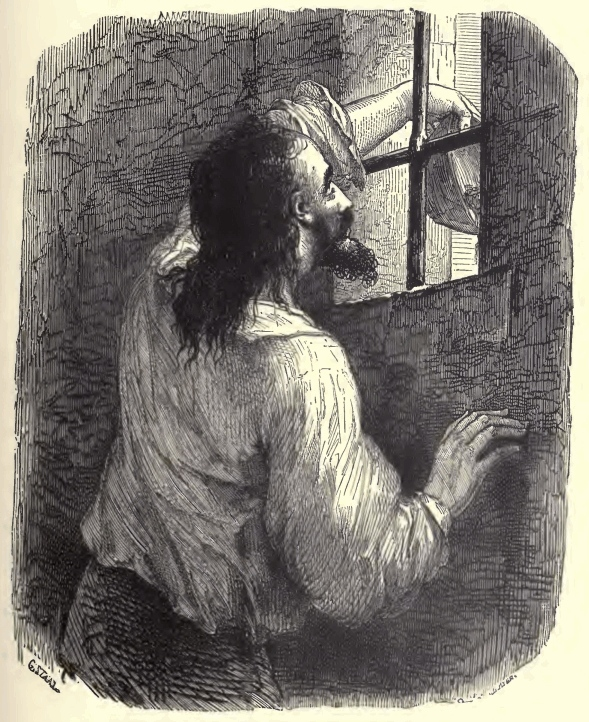
\includegraphics[width=\textwidth]{0185m.jpg}
\end{figure}

Nearly four years had passed away; at the end of the second he had
ceased to mark the lapse of time. Dantès said, “I wish to die,” and had
chosen the manner of his death, and fearful of changing his mind, he
had taken an oath to die. “When my morning and evening meals are
brought,” thought he, “I will cast them out of the window, and they
will think that I have eaten them.”

He kept his word; twice a day he cast out, through the barred aperture,
the provisions his jailer brought him—at first gayly, then with
deliberation, and at last with regret. Nothing but the recollection of
his oath gave him strength to proceed. Hunger made viands once
repugnant, now acceptable; he held the plate in his hand for an hour at
a time, and gazed thoughtfully at the morsel of bad meat, of tainted
fish, of black and mouldy bread. It was the last yearning for life
contending with the resolution of despair; then his dungeon seemed less
sombre, his prospects less desperate. He was still young—he was only
four or five-and-twenty—he had nearly fifty years to live. What
unforseen events might not open his prison door, and restore him to
liberty? Then he raised to his lips the repast that, like a voluntary
Tantalus, he refused himself; but he thought of his oath, and he would
not break it. He persisted until, at last, he had not sufficient
strength to rise and cast his supper out of the loophole. The next
morning he could not see or hear; the jailer feared he was dangerously
ill. Edmond hoped he was dying.

Thus the day passed away. Edmond felt a sort of stupor creeping over
him which brought with it a feeling almost of content; the gnawing pain
at his stomach had ceased; his thirst had abated; when he closed his
eyes he saw myriads of lights dancing before them like the
will-o’-the-wisps that play about the marshes. It was the twilight of
that mysterious country called Death!

Suddenly, about nine o’clock in the evening, Edmond heard a hollow
sound in the wall against which he was lying.

So many loathsome animals inhabited the prison, that their noise did
not, in general, awake him; but whether abstinence had quickened his
faculties, or whether the noise was really louder than usual, Edmond
raised his head and listened. It was a continual scratching, as if made
by a huge claw, a powerful tooth, or some iron instrument attacking the
stones.

Although weakened, the young man’s brain instantly responded to the
idea that haunts all prisoners—liberty! It seemed to him that heaven
had at length taken pity on him, and had sent this noise to warn him on
the very brink of the abyss. Perhaps one of those beloved ones he had
so often thought of was thinking of him, and striving to diminish the
distance that separated them.

No, no, doubtless he was deceived, and it was but one of those dreams
that forerun death!

Edmond still heard the sound. It lasted nearly three hours; he then
heard a noise of something falling, and all was silent.

Some hours afterwards it began again, nearer and more distinct. Edmond
was intensely interested. Suddenly the jailer entered.

For a week since he had resolved to die, and during the four days that
he had been carrying out his purpose, Edmond had not spoken to the
attendant, had not answered him when he inquired what was the matter
with him, and turned his face to the wall when he looked too curiously
at him; but now the jailer might hear the noise and put an end to it,
and so destroy a ray of something like hope that soothed his last
moments.

The jailer brought him his breakfast. Dantès raised himself up and
began to talk about everything; about the bad quality of the food,
about the coldness of his dungeon, grumbling and complaining, in order
to have an excuse for speaking louder, and wearying the patience of his
jailer, who out of kindness of heart had brought broth and white bread
for his prisoner.

Fortunately, he fancied that Dantès was delirious; and placing the food
on the rickety table, he withdrew. Edmond listened, and the sound
became more and more distinct.

“There can be no doubt about it,” thought he; “it is some prisoner who
is striving to obtain his freedom. Oh, if I were only there to help
him!”

Suddenly another idea took possession of his mind, so used to
misfortune, that it was scarcely capable of hope—the idea that the
noise was made by workmen the governor had ordered to repair the
neighboring dungeon.

It was easy to ascertain this; but how could he risk the question? It
was easy to call his jailer’s attention to the noise, and watch his
countenance as he listened; but might he not by this means destroy
hopes far more important than the short-lived satisfaction of his own
curiosity? Unfortunately, Edmond’s brain was still so feeble that he
could not bend his thoughts to anything in particular. He saw but one
means of restoring lucidity and clearness to his judgment. He turned
his eyes towards the soup which the jailer had brought, rose, staggered
towards it, raised the vessel to his lips, and drank off the contents
with a feeling of indescribable pleasure.

He had the resolution to stop with this. He had often heard that
shipwrecked persons had died through having eagerly devoured too much
food. Edmond replaced on the table the bread he was about to devour,
and returned to his couch—he did not wish to die. He soon felt that his
ideas became again collected—he could think, and strengthen his
thoughts by reasoning. Then he said to himself:

“I must put this to the test, but without compromising anybody. If it
is a workman, I need but knock against the wall, and he will cease to
work, in order to find out who is knocking, and why he does so; but as
his occupation is sanctioned by the governor, he will soon resume it.
If, on the contrary, it is a prisoner, the noise I make will alarm him,
he will cease, and not begin again until he thinks everyone is asleep.”

Edmond rose again, but this time his legs did not tremble, and his
sight was clear; he went to a corner of his dungeon, detached a stone,
and with it knocked against the wall where the sound came. He struck
thrice.

At the first blow the sound ceased, as if by magic.

Edmond listened intently; an hour passed, two hours passed, and no
sound was heard from the wall—all was silent there.

Full of hope, Edmond swallowed a few mouthfuls of bread and water, and,
thanks to the vigor of his constitution, found himself well-nigh
recovered.

The day passed away in utter silence—night came without recurrence of
the noise.

“It is a prisoner,” said Edmond joyfully. His brain was on fire, and
life and energy returned.

The night passed in perfect silence. Edmond did not close his eyes.

In the morning the jailer brought him fresh provisions—he had already
devoured those of the previous day; he ate these listening anxiously
for the sound, walking round and round his cell, shaking the iron bars
of the loophole, restoring vigor and agility to his limbs by exercise,
and so preparing himself for his future destiny. At intervals he
listened to learn if the noise had not begun again, and grew impatient
at the prudence of the prisoner, who did not guess he had been
disturbed by a captive as anxious for liberty as himself.

Three days passed—seventy-two long tedious hours which he counted off
by minutes!

At length one evening, as the jailer was visiting him for the last time
that night, Dantès, with his ear for the hundredth time at the wall,
fancied he heard an almost imperceptible movement among the stones. He
moved away, walked up and down his cell to collect his thoughts, and
then went back and listened.

The matter was no longer doubtful. Something was at work on the other
side of the wall; the prisoner had discovered the danger, and had
substituted a lever for a chisel.

Encouraged by this discovery, Edmond determined to assist the
indefatigable laborer. He began by moving his bed, and looked around
for anything with which he could pierce the wall, penetrate the moist
cement, and displace a stone.

He saw nothing, he had no knife or sharp instrument, the window grating
was of iron, but he had too often assured himself of its solidity. All
his furniture consisted of a bed, a chair, a table, a pail, and a jug.
The bed had iron clamps, but they were screwed to the wood, and it
would have required a screw-driver to take them off. The table and
chair had nothing, the pail had once possessed a handle, but that had
been removed.

\begin{figure}[h]
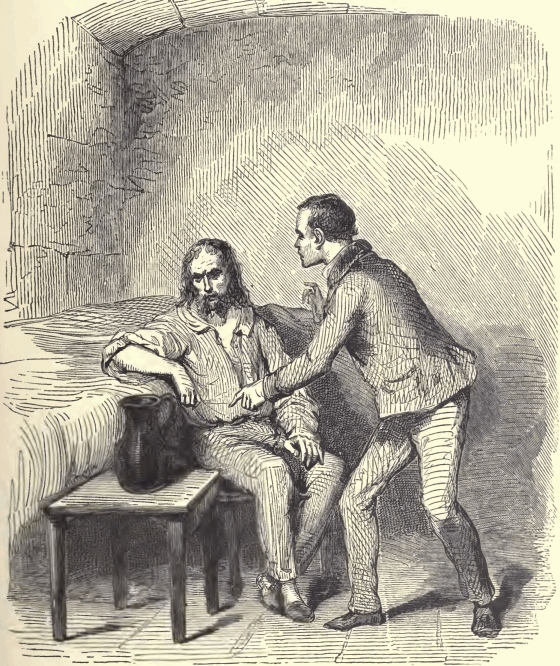
\includegraphics[width=\textwidth]{0189m.jpg}
\end{figure}

Dantès had but one resource, which was to break the jug, and with one
of the sharp fragments attack the wall. He let the jug fall on the
floor, and it broke in pieces.

Dantès concealed two or three of the sharpest fragments in his bed,
leaving the rest on the floor. The breaking of his jug was too natural
an accident to excite suspicion. Edmond had all the night to work in,
but in the darkness he could not do much, and he soon felt that he was
working against something very hard; he pushed back his bed, and waited
for day.

All night he heard the subterranean workman, who continued to mine his
way. Day came, the jailer entered. Dantès told him that the jug had
fallen from his hands while he was drinking, and the jailer went
grumblingly to fetch another, without giving himself the trouble to
remove the fragments of the broken one. He returned speedily, advised
the prisoner to be more careful, and departed.

Dantès heard joyfully the key grate in the lock; he listened until the
sound of steps died away, and then, hastily displacing his bed, saw by
the faint light that penetrated into his cell, that he had labored
uselessly the previous evening in attacking the stone instead of
removing the plaster that surrounded it.

The damp had rendered it friable, and Dantès was able to break it
off—in small morsels, it is true, but at the end of half an hour he had
scraped off a handful; a mathematician might have calculated that in
two years, supposing that the rock was not encountered, a passage
twenty feet long and two feet broad, might be formed.

The prisoner reproached himself with not having thus employed the hours
he had passed in vain hopes, prayer, and despondency. During the six
years that he had been imprisoned, what might he not have accomplished?

This idea imparted new energy, and in three days he had succeeded, with
the utmost precaution, in removing the cement, and exposing the
stone-work. The wall was built of rough stones, among which, to give
strength to the structure, blocks of hewn stone were at intervals
imbedded. It was one of these he had uncovered, and which he must
remove from its socket.

Dantès strove to do this with his nails, but they were too weak. The
fragments of the jug broke, and after an hour of useless toil, Dantès
paused with anguish on his brow.

Was he to be thus stopped at the beginning, and was he to wait inactive
until his fellow workman had completed his task? Suddenly an idea
occurred to him—he smiled, and the perspiration dried on his forehead.

The jailer always brought Dantès’ soup in an iron saucepan; this
saucepan contained soup for both prisoners, for Dantès had noticed that
it was either quite full, or half empty, according as the turnkey gave
it to him or to his companion first.

The handle of this saucepan was of iron; Dantès would have given ten
years of his life in exchange for it.

\begin{figure}[ht]
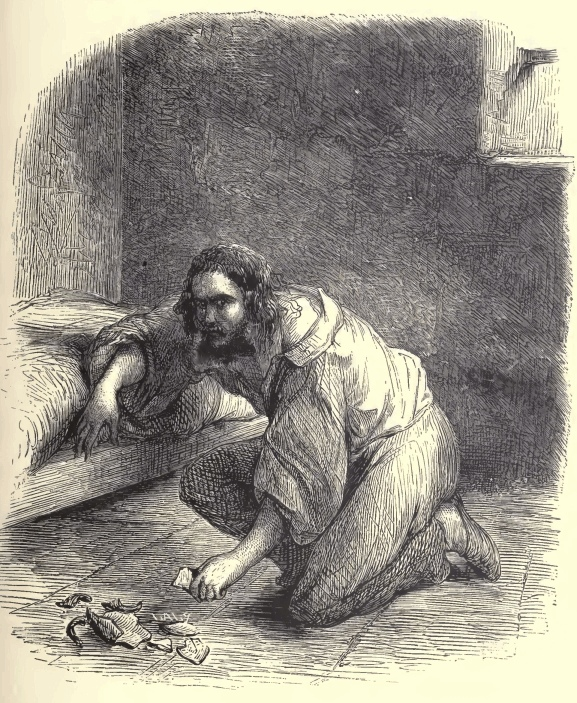
\includegraphics[width=\textwidth]{0191m.jpg}
\end{figure}

The jailer was accustomed to pour the contents of the saucepan into
Dantès’ plate, and Dantès, after eating his soup with a wooden spoon,
washed the plate, which thus served for every day. Now when evening
came Dantès put his plate on the ground near the door; the jailer, as
he entered, stepped on it and broke it.

This time he could not blame Dantès. He was wrong to leave it there,
but the jailer was wrong not to have looked before him. The jailer,
therefore, only grumbled. Then he looked about for something to pour
the soup into; Dantès’ entire dinner service consisted of one
plate—there was no alternative.

“Leave the saucepan,” said Dantès; “you can take it away when you bring
me my breakfast.”

This advice was to the jailer’s taste, as it spared him the necessity
of making another trip. He left the saucepan.

Dantès was beside himself with joy. He rapidly devoured his food, and
after waiting an hour, lest the jailer should change his mind and
return, he removed his bed, took the handle of the saucepan, inserted
the point between the hewn stone and rough stones of the wall, and
employed it as a lever. A slight oscillation showed Dantès that all
went well. At the end of an hour the stone was extricated from the
wall, leaving a cavity a foot and a half in diameter.

Dantès carefully collected the plaster, carried it into the corner of
his cell, and covered it with earth. Then, wishing to make the best use
of his time while he had the means of labor, he continued to work
without ceasing. At the dawn of day he replaced the stone, pushed his
bed against the wall, and lay down. The breakfast consisted of a piece
of bread; the jailer entered and placed the bread on the table.

“Well, don’t you intend to bring me another plate?” said Dantès.

“No,” replied the turnkey; “you destroy everything. First you break
your jug, then you make me break your plate; if all the prisoners
followed your example, the government would be ruined. I shall leave
you the saucepan, and pour your soup into that. So for the future I
hope you will not be so destructive.”

Dantès raised his eyes to heaven and clasped his hands beneath the
coverlet. He felt more gratitude for the possession of this piece of
iron than he had ever felt for anything. He had noticed, however, that
the prisoner on the other side had ceased to labor; no matter, this was
a greater reason for proceeding—if his neighbor would not come to him,
he would go to his neighbor. All day he toiled on untiringly, and by
the evening he had succeeded in extracting ten handfuls of plaster and
fragments of stone. When the hour for his jailer’s visit arrived,
Dantès straightened the handle of the saucepan as well as he could, and
placed it in its accustomed place. The turnkey poured his ration of
soup into it, together with the fish—for thrice a week the prisoners
were deprived of meat. This would have been a method of reckoning time,
had not Dantès long ceased to do so. Having poured out the soup, the
turnkey retired.

Dantès wished to ascertain whether his neighbor had really ceased to
work. He listened—all was silent, as it had been for the last three
days. Dantès sighed; it was evident that his neighbor distrusted him.
However, he toiled on all the night without being discouraged; but
after two or three hours he encountered an obstacle. The iron made no
impression, but met with a smooth surface; Dantès touched it, and found
that it was a beam. This beam crossed, or rather blocked up, the hole
Dantès had made; it was necessary, therefore, to dig above or under it.
The unhappy young man had not thought of this.

“Oh, my God, my God!” murmured he, “I have so earnestly prayed to you,
that I hoped my prayers had been heard. After having deprived me of my
liberty, after having deprived me of death, after having recalled me to
existence, my God, have pity on me, and do not let me die in despair!”

\begin{figure}[ht]
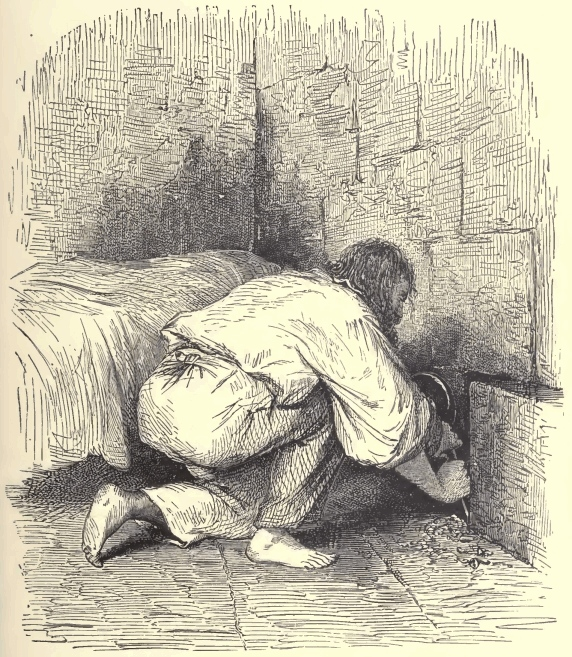
\includegraphics[width=\textwidth]{0193m.jpg}
\end{figure}

“Who talks of God and despair at the same time?” said a voice that
seemed to come from beneath the earth, and, deadened by the distance,
sounded hollow and sepulchral in the young man’s ears. Edmond’s hair
stood on end, and he rose to his knees.

“Ah,” said he, “I hear a human voice.” Edmond had not heard anyone
speak save his jailer for four or five years; and a jailer is no man to
a prisoner—he is a living door, a barrier of flesh and blood adding
strength to restraints of oak and iron.

“In the name of Heaven,” cried Dantès, “speak again, though the sound
of your voice terrifies me. Who are you?”

“Who are you?” said the voice.

“An unhappy prisoner,” replied Dantès, who made no hesitation in
answering.

“Of what country?”

“A Frenchman.”

“Your name?”

“Edmond Dantès.”

“Your profession?”

“A sailor.”

“How long have you been here?”

“Since the 28th of February, 1815.”

“Your crime?”

“I am innocent.”

“But of what are you accused?”

“Of having conspired to aid the emperor’s return.”

“What! For the emperor’s return?—the emperor is no longer on the
throne, then?”

“He abdicated at Fontainebleau in 1814, and was sent to the Island of
Elba. But how long have you been here that you are ignorant of all
this?”

“Since 1811.”

Dantès shuddered; this man had been four years longer than himself in
prison.

“Do not dig any more,” said the voice; “only tell me how high up is
your excavation?”

“On a level with the floor.”

“How is it concealed?”

“Behind my bed.”

“Has your bed been moved since you have been a prisoner?”

“No.”

“What does your chamber open on?”

“A corridor.”

“And the corridor?”

“On a court.”

“Alas!” murmured the voice.

“Oh, what is the matter?” cried Dantès.

“I have made a mistake owing to an error in my plans. I took the wrong
angle, and have come out fifteen feet from where I intended. I took the
wall you are mining for the outer wall of the fortress.”

“But then you would be close to the sea?”

“That is what I hoped.”

“And supposing you had succeeded?”

“I should have thrown myself into the sea, gained one of the islands
near here—the Isle de Daume or the Isle de Tiboulen—and then I should
have been safe.”

“Could you have swum so far?”

“Heaven would have given me strength; but now all is lost.”

“All?”

“Yes; stop up your excavation carefully, do not work any more, and wait
until you hear from me.”

“Tell me, at least, who you are?”

“I am—I am No. 27.”

“You mistrust me, then,” said Dantès. Edmond fancied he heard a bitter
laugh resounding from the depths.

“Oh, I am a Christian,” cried Dantès, guessing instinctively that this
man meant to abandon him. “I swear to you by him who died for us that
naught shall induce me to breathe one syllable to my jailers; but I
conjure you do not abandon me. If you do, I swear to you, for I have
got to the end of my strength, that I will dash my brains out against
the wall, and you will have my death to reproach yourself with.”

“How old are you? Your voice is that of a young man.”

“I do not know my age, for I have not counted the years I have been
here. All I do know is, that I was just nineteen when I was arrested,
the 28th of February, 1815.”

“Not quite twenty-six!” murmured the voice; “at that age he cannot be a
traitor.”

“Oh, no, no,” cried Dantès. “I swear to you again, rather than betray
you, I would allow myself to be hacked in pieces!”

“You have done well to speak to me, and ask for my assistance, for I
was about to form another plan, and leave you; but your age reassures
me. I will not forget you. Wait.”

“How long?”

“I must calculate our chances; I will give you the signal.”

“But you will not leave me; you will come to me, or you will let me
come to you. We will escape, and if we cannot escape we will talk; you
of those whom you love, and I of those whom I love. You must love
somebody?”

“No, I am alone in the world.”

“Then you will love me. If you are young, I will be your comrade; if
you are old, I will be your son. I have a father who is seventy if he
yet lives; I only love him and a young girl called Mercédès. My father
has not yet forgotten me, I am sure, but God alone knows if she loves
me still; I shall love you as I loved my father.”

“It is well,” returned the voice; “tomorrow.”

These few words were uttered with an accent that left no doubt of his
sincerity; Dantès rose, dispersed the fragments with the same
precaution as before, and pushed his bed back against the wall. He then
gave himself up to his happiness. He would no longer be alone. He was,
perhaps, about to regain his liberty; at the worst, he would have a
companion, and captivity that is shared is but half captivity. Plaints
made in common are almost prayers, and prayers where two or three are
gathered together invoke the mercy of heaven.

All day Dantès walked up and down his cell. He sat down occasionally on
his bed, pressing his hand on his heart. At the slightest noise he
bounded towards the door. Once or twice the thought crossed his mind
that he might be separated from this unknown, whom he loved already;
and then his mind was made up—when the jailer moved his bed and stooped
to examine the opening, he would kill him with his water jug. He would
be condemned to die, but he was about to die of grief and despair when
this miraculous noise recalled him to life.

The jailer came in the evening. Dantès was on his bed. It seemed to him
that thus he better guarded the unfinished opening. Doubtless there was
a strange expression in his eyes, for the jailer said, “Come, are you
going mad again?”

Dantès did not answer; he feared that the emotion of his voice would
betray him. The jailer went away shaking his head. Night came; Dantès
hoped that his neighbor would profit by the silence to address him, but
he was mistaken. The next morning, however, just as he removed his bed
from the wall, he heard three knocks; he threw himself on his knees.

“Is it you?” said he; “I am here.”

“Is your jailer gone?”

“Yes,” said Dantès; “he will not return until the evening; so that we
have twelve hours before us.”

“I can work, then?” said the voice.

“Oh, yes, yes; this instant, I entreat you.”

In a moment that part of the floor on which Dantès was resting his two
hands, as he knelt with his head in the opening, suddenly gave way; he
drew back smartly, while a mass of stones and earth disappeared in a
hole that opened beneath the aperture he himself had formed. Then from
the bottom of this passage, the depth of which it was impossible to
measure, he saw appear, first the head, then the shoulders, and lastly
the body of a man, who sprang lightly into his cell.

\begin{figure}[h]
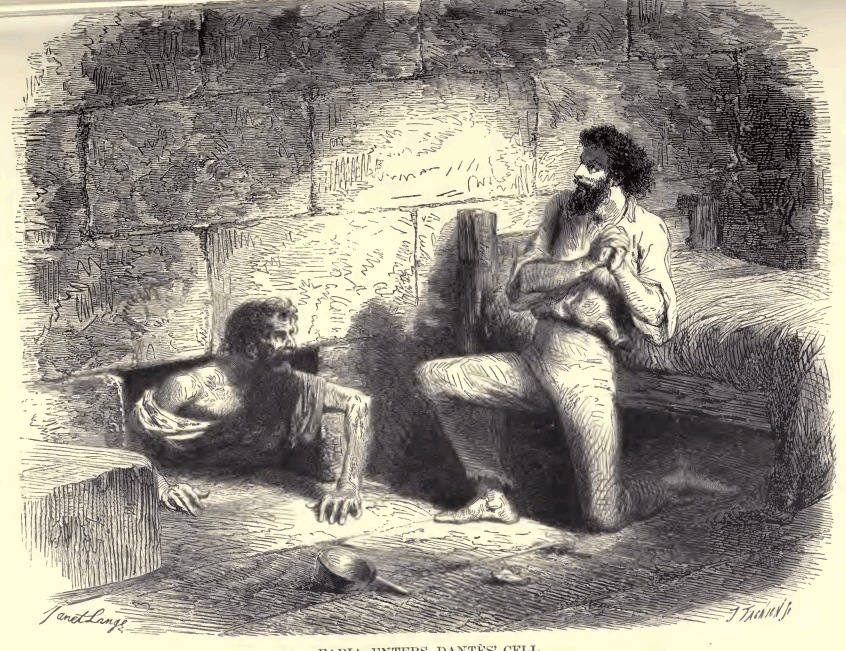
\includegraphics[width=\textwidth]{0197m.jpg}
\end{figure}

\chapter{ADAM'S PLACE IN THE EARTH'S DESTINY—2}

IN the Doctrine and Covenants, Section 107, we have a wonderful revelation on Priesthood.
This revelation was given at the request of the recently ordained apostles. They were about to
go forth on missions assigned to them and they desired some guidance by revelation, so the
Lord granted this request and instructed them in matters pertaining to the Priesthood. In the
course of this divine communication the Lord gave definite instruction in relation to Adam
and the patriarchs living before the flood. In it we are informed that the Priesthood was first
given to Adam and he in the course of years, ordained his son Seth, Enos, Cainan,
Mahalaleel, Jared, Enoch and Methuselah. Be it remembered that Adam, after the fall, lived
for 930 years. Seth ordained Lamech and Noah was ordained by Methuselah. This is the
descent of Priesthood from the beginning to the time of the flood.

Three years before the death of Adam, or in the year 927 from the date of the fall, this great
Patriarch and father of the human family called Seth, Enos, Cainan, Mahaleel, Jared, Enoch
and Methuselah, who were all high priests, with the residue of his faithful descendants, now
numerous, into the valley of Adam-ondi-Ahman, the place where Adam dwelt, and there
bestowed upon them his last blessing.

And the Lord appeared unto them, and they rose up and blessed Adam, and called him
Michael, the prince, the archangel.

And the Lord administered comfort unto Adam, and said unto him: I have set thee to be at
the head; a multitude of nations shall come of thee, and thou art a prince over them forever.

And Adam stood up in the midst of the congregation; and, notwithstanding he was bowed
down with age, being full of the Holy Ghost, predicted whatsoever should befall his posterity
unto the latest generation.

These things were all written in the book of Enoch, and are to be testified of in due time. 1

Again in Section 84, we have another reference to the descent of the Priesthood, this time
tracing it back from Moses, Abraham, Melchizedek, Noah, Enoch, Able to Adam, and in
verses 16 and 17 we read:

And from Enoch to Abel, who was slain by the conspiracy of his brother, who received the
priesthood by the commandments of God, by the hand of his father Adam, \textit{who was the first
man—}

Which priesthood continueth in the church of God in all generations, and is without
beginning of days or end of years.

We are here informed again that Adam was the first man, and that the Priesthood held by the
prophets of old came down through his lineage from him to the days of Moses, and from
Moses it continued on to the days of the coming of our Lord and Savior Jesus Christ. In the
Doctrine and Covenants, Section 117, we are informed that Adam dwelt in Adam-ondi-Ahman and the plains of Olaha Shinehah, which places have been made known to have been
on the western hemisphere, and in what is now known as the State of Missouri. This is well
for us to remember since it is the general impression that civilization commenced on the
eastern hemisphere. Then, in a revelation given to President Brigham Young at Winter
Quarters, January 14, 1847, the Lord said:

For they killed the prophets, and them that were sent unto them; and they have shed innocent
blood, which crieth from the ground against them.

Therefore, marvel not at these things, for ye are not yet pure; ye cannot yet bear my glory;
but ye shall behold it if ye are faithful in keeping all my words that I have given you, from
the days of Adam to Abraham, from Abraham to Moses, from Moses to Jesus and his
apostles, and from Jesus and his apostles to Joseph Smith, whom I did call upon by mine
angels, my ministering servants, and by mine own voice out of the heavens, to bring forth my
work. 2

I have now given testimony from the Pearl of Great Price, the Book of Mormon and the
Doctrine and Covenants, all confirming what is written in the Bible in regard to Adam, his
creation, his fall, his Priesthood, and indicating to us a very definite time when he lived; of
his ministry and when he died in full fellowship with the Lord, honored by his righteous
posterity. One other passage completes this list, that from Section 78, verses 15-16:

That you may come up unto the crown prepared for you, and be made rulers over many
kingdoms, saith the Lord God, the Holy One of Zion, who hath established the foundations of
Adam-ondi-Ahman; Who hath appointed Michael your prince, and established his feet, and
set him upon high, and given unto him the keys of salvation under the counsel and direction
of the Holy One, who is without beginning of days or end of life.

In this scripture we receive the knowledge that Michael, who is Adam, not only stands at the
head ruling over his posterity as a prince unto them forever; but also he has been appointed to
hold the keys of salvation for the benefit of the people of all the world who will truly repent
and receive the Gospel, and this great honor is bestowed upon him to act under the direction
of Jesus Christ who is the Only Begotten Son of God and the Holy One of Israel. Therefore,
all ye mockers and you mighty men take heed unto yourselves, for the day will come when
you will have to face this first man who has been crowned with honor to stand next to Jesus
Christ holding the keys of salvation; and you will not pass through the gates into that
kingdom without his consent! When that day comes and if you are permitted to pass through
those gates it will be only because you sorely repented and have humbly apologized to this
great man whom you have so mercilessly maligned.

The following teachings in regard to Adam are taken from the discourses and writings of the
Prophet Joseph Smith, who was better prepared to speak than any other man since the days of
Jesus Christ, on the life and authority of Adam. His knowledge was not obtained from books
or the writings of the worldly wise of the present day. What he learned and revealed was
given him by divine revelation.

The Prophet Joseph Smith had this to say about Adam and the Priesthood:

The Priesthood was first given to Adam; he obtained the First Presidency, and held the keys
of it from generation to generation. He obtained it in the Creation, before the world was
formed, as in Genesis 1:26, 27, 28. He had dominion given him over every living creature.
He is Michael the Archangel, spoken of in the scriptures. Then to Noah, who is Gabriel; he
stands next in authority to Adam in the Priesthood; he was called of God to this office, and
was the father of all living in his day, and to him was given the dominion. These men held
keys first on earth, and then in heaven.

The Priesthood is an everlasting principle, and existed with God from eternity, and will to
eternity, without beginning of days or end of years. The keys have to be brought from heaven
whenever the Gospel is sent. When they are revealed from heaven, it is by Adam's authority.

Daniel in his seventh chapter speaks of the Ancient of Days; he means the oldest man, our
Father Adam, Michael, he will call his children together and hold a council with them to
prepare them for the coming of the Son of Man. He (Adam) is the father of the human
family, and presides over the spirits of all men, and all that have had the keys must stand
before him in this grand council. This may take place before some of us leave this stage of
action. The Son of Man stands before him, and here is given him glory and dominion. Adam
delivers up his stewardship to Christ, that which was delivered to him as holding the keys of
the universe, but retains his standing as head of the human family.

The spirit of man is not a created being; it existed from eternity, and will exist to eternity.
Anything created cannot be eternal; and earth, water, etc., had their existence in an
elementary state, from eternity. Our Savior speaks of children and says, Their angels always
stand before my Father. The Father called all spirits before him at the creation of man, and
organized them. He (Adam) is the head and was told to multiply. The keys were first given to
him, and by him to others. He will have to give an account of his stewardship, and they to
him.

The Priesthood is everlasting. The Savior, Moses, and Elias, gave the keys to Peter, James
and John, on the mount, when they were transfigured before him. The Priesthood is
everlasting—without beginning of days or end of years; without father, mother, etc. If there
is no change of ordinances, there is no change of Priesthood. Wherever the ordinances of the
Gospel are administered, there is the Priesthood.

DESCENT OF PRIESTHOOD

How have we come at the Priesthood in the last days? It came down, in regular succession.
Peter, James and John, had it given to them and they gave it to others. Christ is the Great
High Priest; Adam next. Paul speaks of the Church coming to an innumerable company of
angels . . . to God the Judge of all—the spirits of just men made perfect; to Jesus the mediator
of the new covenant. (Hebrews 12:23.)

I saw Adam in the valley of Adam-ondi-Ahman. He called together his children and blessed
them with a patriarchal blessing. The Lord appeared in their midst, and he (Adam) blessed
them all, and foretold what would befall them to the latest generation.

This is why Adam blessed his posterity; he wanted to bring them into the presence of God.
They looked for a city, etc., "whose builder and maker is God." (Hebrews 11:10.) Mosessought to bring the children of Israel into the presence of God, through the power of the
Priesthood, but he could not. \textit{In the first ages of the world} they tried to establish the same
thing; and there were Eliases raised up who tried to restore these very glories, but did not
obtain them; but they prophesied of a day when this glory would be revealed. Paul spoke of
the dispensation of the fulness of times, when God would gather together all things in one,
etc.; and those men to whom these keys have been given, will have to be there; and they
without us cannot be made perfect.

These men are in heaven, but their children are on the earth. Their bowels yearn over us. God
sends down men for this reason. "The Son of man shall send forth his angels, and they shall
gather out of his kingdom all things that offend, and them which do iniquity." (Matthew
13:41.) All these authoritative characters will come down and join hand in hand in bringing
about this work. 3

At the October conference in Nauvoo in 1840, the Prophet gave further instruction regarding
the Priesthood and in the course of his remarks had the following to say about Adam:

Commencing with Adam, who was the first man, who is spoken of in Daniel as being the
"Ancient of Days," or in other words, the first and oldest of all, the great, grand progenitor of
whom it is said in another place he is Michael, because he was the first and father of all, not
only by progeny, but the first to hold the spiritual blessings, to whom was made known the
plan of ordinances for the salvation of his posterity unto the end, and to whom Christ was
first revealed, and through whom Christ has been revealed from heaven, and will continue to
be revealed from henceforth. Adam holds the keys of the dispensation of the fulness of times;
i.e., the dispensation of all the times have been and will be revealed through him from the
beginning to Christ, and from Christ to the end of the dispensations that are to be revealed.
"Having made known unto us the mystery of his will, according to his good pleasure which
he hath purposed in himself: That in the dispensation of the fulness of times he might gather
together in one all things in Christ, both which are in heaven, and which are on earth; even in
him." (Eph. 1:9-10.)

Now the purpose in himself in the winding up scene of the last dispensation is that all things
pertaining to that dispensation should be conducted precisely in accordance with the
preceding dispensations.

And again, God purposed in himself that there should not be an eternal fulness until every
dispensation should be fulfilled and gathered together in one, and that all things whatever,
that should be gathered together in one in those dispensations unto the same fulness and
eternal glory, should be in Christ Jesus; therefore he set the ordinances to be the same forever
and ever, and set Adam to watch over them, to reveal them from heaven to man, or to send
angels to reveal them. "Are they not all ministering spirits, sent forth to minister for them
who shall be heirs of salvation?" (Hebrews 1:14.)

These angels are under the direction of Michael or Adam, who acts under the direction of the
Lord. From the above quotation we learn that Paul perfectly understood the purposes of God
in relation to his connection with man, and that glorious and perfect order which he
established in himself, whereby he sent forth power, revelations, and glory.

ADAM RECEIVED COMMANDMENTS FROM GOD

God will not acknowledge that which he has not called, ordained, and chosen. In the
beginning God called Adam by his own voice. "And the Lord God called unto Adam, and
said unto him, Where art thou? And he said, I heard thy voice in the garden, and I was afraid
because I was naked; and hid myself." (Genesis 3:9-10.) Adam received commandments and
instructions from God: this was the order from the beginning.

That he received revelations, commandments and ordinances at the beginning is beyond the
power of controversy; else how did they begin to offer sacrifices to God in an acceptable
manner. And if they offered sacrifices they must be authorized by ordination. We read in
Genesis 4:4, that Abel brought of the firstlings of the flock and the fat thereof, and the Lord
had respect to Abel and to his offering. And, again, "By faith Abel offered unto God a more
excellent sacrifice than Cain, by which he obtained witness that he was righteous, God
testifying of his gifts: and by it he being dead yet speaketh." (Hebrews 11:4.) How doth he
yet speak? Why he magnified the Priesthood which was conferred upon him, and died a
righteous man, and therefore has become an angel of God by receiving his body from the
dead, holding still the keys of his dispensation; and was sent down from heaven unto Paul to
minister consoling words, and to commit unto him a knowledge of the mysteries of
godliness.

And if this was not the case, I would ask, how did Paul know so much about Abel, and why
should he talk about his speaking after he was dead? Hence, that he spoke after he was dead
must be by being sent down out of heaven to administer.

This, then, is the nature of the Priesthood; every man holding the Presidency of his
dispensation, and one man holding the Presidency of them all, even Adam; and Adam
receiving his Presidency and authority from the Lord, but cannot receive a fulness until
Christ shall present the kingdom to the Father, which shall be at the end of the last
dispensation. . . .

If Cain had fulfilled the law of righteousness as did Enoch, he could have walked with God
all the days of his life, and never failed of a blessing. "And Enoch walked with God after he
begat Methuselah three hundred years, and begat sons and daughters: And all the days of
Enoch were three hundred sixty and five years: And Enoch walked with God, and he was not,
for God took him." (Gen. 5:22-24.) Now this Enoch God reserved unto himself, that he
should not die at that time, and appointed unto him a ministry unto terrestrial bodies, of
whom there has been little revealed. He is reserved also unto the presidency of a
dispensation, and more shall be said of him and terrestrial bodies in another treatise. He is a
ministering angel, to minister to those who shall be heirs of salvation, and appeared unto
Jude as Abel did unto Paul; therefore Jude spoke of him (14-15 verses). And Enoch, the
seventh from Adam, revealed these sayings: "Behold, the Lord cometh with ten thousands of
his saints." 4

In the early part of the year 1912, Elder Samuel O. Bennion, then presiding in the Central
States Mission, wrote to the First Presidency for a statement answering the enemies of the
Church who were falsely quoting President Brigham Young. The letter of Presidency to
Elder Bennion is as follows:

Salt Lake City, Utah

February 20, 1912

Pres. Samuel O. Bennion,

Independence, Missouri.

Dear Brother:

Your question concerning Adam has not been answered because of pressure of important
business. We now respond briefly but, we hope, plainly. You speak of "the assertion made by
Brigham Young that Jesus was begotten of the Father in the flesh by our father Adam, and
that Adam is the father of Jesus Christ and not the Holy Ghost, and you say that elders are
challenged by certain critics to prove this.

If you will carefully examine the sermon to which you refer, in the \textit{Journal of Discourses,}
Vol. 1, you will discover that, while President Young denied that Jesus was "begotten by the
Holy Ghost," he did not affirm, in so many words, that "Adam is the father of Jesus Christ in
the flesh." He said, "Jesus, our elder brother, was begotten in the flesh by the same character
that was in the garden of Eden and who is our Father in Heaven." Here is what President
Young said about him, "Our Father in Heaven begat all the spirits that ever were or ever will
be upon this earth and they were born spirits in the eternal world. Then the Lord by his power
and wisdom organized the mortal tabernacle of man." Was he in the garden of Eden?

Surely; he gave commandment to Adam and Eve; he was their Father in Heaven; they
worshiped him and taught their children after the fall to worship and obey him in the name of
the Son who was to come.

But President Young went on to show that our father Adam—that is, our earthly father—the
progenitor of the race of man, stands at the head, being "Michael the Archangel, the Ancient
of Days," and that he was not fashioned from earth like an adobe, but begotten by his Father
in Heaven.

Adam is called in the Bible "the son of God." (Luke 3:38.) It was our Father in Heaven who
begat the spirit of him who was the Firstborn of all spirits that come to this earth and who
was also his Father by the Virgin Mary, making him "the Only Begotten in the flesh." Read
Luke 1:26-35. Where is Jesus called "the Only Begotten of the Holy Ghost?" He is always
singled out as "the Only Begotten of the Father." (John 14:3-16-18, etc.). The Holy Ghost
came upon Mary, her conception was under that influence, even of the spirit of life; our
Father in Heaven was the Father of the Son of Mary, to whom the Savior prayed, as did our
earthly father Adam.

When President Young asked, "Who is the father?" he was speaking of Adam as the father of
our earthly bodies, who is at our head as revealed in Doctrine and Covenants, Sec. 107,
verses 53-56. In that sense he is one of the Gods referred to in numerous scriptures, and
particularly by Christ. (John 10:34-36.) He is the great Patriarch, the Ancient of Days, who
will stand in his place as "a prince over us forever," and with whom we shall have to do," as
each family will have to do with its head, according to the Holy Patriarchal order. Our father
Adam, perfected and glorified as a God, will be a being who will carry out the behests of the
great Elohim in relation to his posterity.

While, as Paul puts it, There be gods many and lords many (whether in heaven or in earth),
unto us there is but one God the Father, of whom are all things, and one Lord Jesus Christ.
Latter-day Saints worship him and him alone, who is the Father of Jesus Christ, whom he
worshiped, whom Adam worshiped and who is God the Eternal Father of us all.

Your brethren,

Joseph F. Smith

Anthon H. Lund

Charles W. Penrose

First Presidency President Brigham Young has borne testimony concerning Adam and his
place in the world as Michael, the Archangel, who will stand at the head of his posterity
forever having jurisdiction over them under Jesus Christ. In one of his discourses he said:

We are safe in saying that from the day that Adam was created and placed in the garden of
Eden to this day, the plan of salvation and the revelations of the will of God to man are
unchanged, although mankind have not for many ages been favored there-with, in
consequence of apostasy and wickedness. There is no evidence to be found in the Bible that
the Gospel should be one thing in the days of the Israelites, and another in the days of Christ
and his apostles, and another in the 19th century, but, on the contrary, we are instructed that
God is the same in every age, and that his plan of saving his children is the same. The plan of
salvation is one, from the beginning of the world to the end thereof. 5

Adam was as conversant with his Father who placed him upon the earth as we are conversant
with our earthly parents. The Father frequently came to visit his son Adam, and walked with
him; and the children of Adam were more or less acquainted with him; and the things that
pertain to God and to heaven were as familiar among mankind in the first ages of their
existence on the earth, as these mountains are to our mountain boys, as gardens are to our
wives and children, or as the road to the Western Ocean is to the experienced traveler. From
this source mankind received their religious traditions. 6

The youth of Israel should remember that the Prophet Joseph Smith was in communication
with the heavens constantly. He was instructed by angels and by the Son of God himself. For
four years he was tutored by the Angel Moroni before he was privileged to obtain the plates
of the Book of Mormon and after that he was frequently visited by heavenly messengers. He
and Oliver Cowdery stood in the presence of John the Baptist and under his hands received
the Aaronic Priesthood, and later under the hands of Peter, James and John received the
Melchizedek Priesthood and were commanded to organize the Church. The ancient prophets
from Adam to Peter, James and John in the dispensation of the Meridian of Time, came and
manifested the keys of their dispensations to these two men. The Prophet Joseph Smith saw
Adam as well as these many other ancient prophets; he speaks by authority for he had the
knowledge. He knew that Adam lived and that he is the "first man," the "Ancient of Days,"
so called because he was the "oldest of all." I have presented the testimonies of the Nephite
prophets, the ancient prophets of the Israelites as the knowledge has come to us through
revelation and recorded in the Pearl of Great Price and the writings of Abraham, all
confirming the stories related in the Bible. We discover that organic evolution mocks at all of
this.

Now, my beloved brethren and sisters, and especially you younger members of the Church, is
it not better to hearken to these brethren who had personal knowledge than to accept the
insecure doctrines of those who reject their Redeemer and his servants and endeavor to put
them to open shame?

\newpage
REFERENCES—CHAPTER SIXTEEN

Footnotes

1. D. \& C. 107:41-57.

2. \textit{Ibid.}, 136:36-37.

3. \textit{Teachings of the Prophet Joseph Smith}, pp. 157-159.

4. \textit{Ibid.}, pp. 167-170.

5. \textit{Journal of Discourses}, Vol. 10, p. 324.

6. \textit{Ibid.}, Vol. 9, p. 148.


\chapter{ADAM'S PLACE IN THE EARTH'S DESTINY—3}

THERE are other testimonies coming from our brethren, who were trained under the
teachings of the Prophet Joseph Smith and who are able to speak by virtue of the inspiration
of the Spirit of the Lord by which they have been led. Their teachings should be heeded by
the members of the Church. The following article by the First Presidency was written for the
purpose of directing our Church members in the light of revealed truth and to fortify them
against the false doctrines and philosophies so prevalent in the world.

THE ORIGIN OF MAN By THE FIRST PRESIDENCY OF THE CHURCH

\textit{"God created man in his own image."}

Inquiries arise from time to time respecting the attitude of the Church of Jesus Christ of
Latter-day Saints upon questions which, though not vital from a doctrinal standpoint, are
closely connected with the fundamental principles of salvation. The latest inquiry of this kind
that has reached us is in relation to the origin of man. It is believed that a statement of the
position held by the Church upon this important subject will be timely and productive of
good.

In presenting the statement that follows we are not conscious of putting forth anything
essentially new; neither is it our desire so to do. Truth is what we wish to present, and truth—
eternal truth—is fundamentally old. A restatement of the original attitude of the Church
relative to this matter is all that will be attempted here. To tell the truth as God has revealed
it, and commend it to the acceptance of those who need to conform their opinions thereto, is
the sole purpose of this presentation.

"God created man in his own image, in the image of God created he him; male and female
created he them." In these plain and pointed words the inspired author of the book of Genesis
made known to the world the truth concerning the origin of the human family. Moses, the
prophet-historian, "learned," as we are told, "in all the wisdom of the Egyptians," when
making this important announcement, was not voicing a mere opinion, a theory derived from
his researches into the occult lore of that ancient people. He was speaking as the mouthpiece
of God, and his solemn declaration was for all time and for all people. No subsequent
revelator of the truth has contradicted the great leader and law-giver of Israel. All who have
since spoken by divine authority upon this theme have confirmed his simple and sublime
proclamation. Nor could it be otherwise. Truth has but one source, and all revelations from
heaven are harmonious with each other. The omnipotent Creator, the maker of heaven and
earth—had shown unto Moses everything pertaining to this planet, including the facts
relating to man's origin, and the authoritative pronouncement of that mighty prophet and seer
to the house of Israel, and through Israel to the whole world, is couched in the simplest
clause: "God created man in his own Image." (Genesis 1:27; Pearl of Great Price—Book of
Moses, 1:27-41.)

The creation was two-fold—first spiritual, secondly temporal. This truth, also, Moses plainly
taught—much more plainly than it has come down to us in the imperfect translations of the
Bible that are now in use. Therein the fact of a spiritual creation, antedating the temporal
creation, is strongly implied, but the proof of it is not so clear and conclusive as in other
records held by the Latter-day Saints to be of equal authority with the Jewish scriptures. The
partial obscurity of the latter upon the point in question is owing, no doubt, to the loss of
those "plain and precious" parts of sacred writ, which, as the Book of Mormon informs us,
have been taken away from the Bible during its passage down the centuries. (1 Nephi 13:24-
29.) Some of these missing parts the Prophet Joseph Smith undertook to restore when he
revised those scriptures by the spirit of revelation, the result being that more complete
account of the creation which is found in the book of Moses, previously cited. Note the
following passages:

"And now, behold I say unto you, that these are the generations of the heaven and of the
earth, when they were created, in the day that I, the Lord God, made the heaven and the
earth:

"And every plant of the field before it was in the earth, and every herb of the field before it
grew. For I, the Lord God, created all things, of which I have spoken, spiritually, before they
were naturally upon the face of the earth. For I, the Lord God, had not caused it to rain upon
the face of the earth. And I, the Lord God, had created all the children of men, and not yet a
man to till the ground: for in heaven created I them; and there was not yet flesh upon the
earth, neither in the water, neither in the air:

"But I, the Lord God, spake, and there went up a mist from the earth, and watered the whole
face of the ground.

"And I, the Lord God, formed man from the dust of the ground, and breathed into his nostrils
the breath of life; and man became a living soul, the first flesh upon the earth, the first man
also; nevertheless, all things were before created; but spiritually were they created and made
according to my word." (Pearl of Great Price—Book of Moses, 3:4-7. See also chapters 1
and 2, and compare with Genesis 1 and 2.)

These two points being established, namely, the creation of man in the image of God, and the
two-fold character of the creation, let us now inquire: What was the form of man, in the spirit
and in the body, as originally created? In a general way the answer is given in the words
chosen as the text of this treatise. "God created man in his own image." It is more explicitly
rendered in the Book of Mormon thus: "All men were created in the beginning after mine
own image." (Ether 3:15.) It is the Father who is speaking. If, therefore, we can ascertain the
form of the "Father of spirits," "The God of the spirits of all flesh," we shall be able to
discover the form of the original man.

Jesus Christ, the Son of God, is "the express image" of his Father's person. (Hebrews 1:3.) He
walked the earth as a human being, as a perfect man, and said, in answer to a question put to
him: "He that hath seen me hath seen the Father." (John 14:9.) This alone ought to solve the
problem to the satisfaction of every thoughtful, reverent mind. The conclusion is irresistible,
that if the Son of God be the express image (that is, likeness) of his Father's person, then his
Father is in the form of man; for that was the form of the Son of God, not only during his
mortal life, but before his mortal birth, and after his resurrection. It was in this form that the
Father and the Son, as two personages, appeared to Joseph Smith, when, as a boy of fourteen
years, he received his first vision. Then if God made man—the first man—in his own image
and likeness, he must have made him like unto Christ, and consequently like unto men of
Christ's time and of the present day. That man was made in the image of Christ, is positively
stated in the book of Moses: "And I, God, said unto mine Only Begotten, which was with me
from the beginning: Let us make man in our image, after our likeness; and it was so. . . . And
I, God, created man in mine own image, in the image of mine Only Begotten created I him;
male and female created I them." (2:26, 27.)

The Father of Jesus is our Father also, Jesus himself taught this truth, when he instructed his
disciples how to pray: "Our Father which art in heaven," etc. Jesus, however, is the Firstborn
among all the sons of God—the first begotten in the spirit, and the Only Begotten in the
flesh. He is our elder brother, and we, like him, are in the image of God. All men and women
are in the similitude of the universal Father and Mother, and are literally the sons and
daughters of Deity.

"God created man in his own image." This is just as true of the spirit as it is of the body,
which is only the clothing of the spirit, its complement; the two together constituting the
soul. The spirit of man is in the form of man, and the spirits of all creatures are in the likeness
of their bodies. This was plainly taught by the Prophet Joseph Smith. (Doctrine and
Covenants, 77:2.)

Here is further evidence of the fact. More than seven hundred years before Moses was shown
the things pertaining to this earth, another great prophet, known to us as the brother of Jared,
was similarly favored by the Lord. He was even permitted to behold the spirit-body of the
foreordained Savior, prior to his incarnation; and so like the body of a man was his spirit in
form and appearance, that the prophet thought he was gazing upon a being of flesh and
blood. He first saw the finger and then the entire body of the Lord—all in the spirit. The
Book of Mormon says of this wonderful manifestation:

"And it came to pass that when the brother of Jared had said these words, behold, the Lord
stretched forth his hand and touched the stones one by one with his finger. And the veil was
taken from off the eyes of the brother of Jared, and he saw the finger of the Lord; and it was
as the finger of a man, like unto flesh and blood; and the brother of Jared fell down before the
Lord, for he was struck with fear.

"And the Lord saw that the brother of Jared had fallen to the earth; and the Lord said unto
him: Arise, why hast thou fallen?

"And he saith unto the Lord: I saw the finger of the Lord, and I feared lest he should smite
me; for I knew not that the Lord had flesh and blood.

"And the Lord said unto him: Because of thy faith thou hast seen that I shall take upon me
flesh and blood; and never has man come before me with such exceeding faith as thou hast;
for were it not so, ye could not have seen my finger. Sawest thou more than this?

"And he answered: Nay; Lord, show thyself unto me.

"And the Lord said unto him: Believest thou the words which I shall speak?

"And he answered: Yea, Lord, I know that thou speakest the truth, for thou art a God of truth,
and canst not lie.

"And when he had said these words, behold, the Lord showed himself unto him, and said:
Because thou knowest these things ye are redeemed from the fall; therefore ye are brought
back into my presence; therefore I show myself unto you.

"Behold, I am he who was prepared from the foundation of the world to redeem my people.
Behold, I am Jesus Christ. I am the Father and the Son. In me shall all mankind have light,
and that eternally, even they who shall believe on my name; and they shall become my sons
and my daughters.

"And never have I showed myself unto man whom I have created, for never has man
believed in me as thou hast. Seest thou that ye are created after mine own image? Yea, even
all men were created in the beginning after mine own image.

"Behold, this body, which ye now behold, is the body of my spirit; and man have I created
after the body of my spirit; and even as I appear unto thee to be in the spirit will I appear unto
my people in the flesh." (Ether 3:6-16.)

What more is needed to convince us that man, both in spirit and in body, is the image and
likeness of God, and that God himself is in the form of man?

When the divine Being whose spirit-body the brother of Jared beheld, took upon him flesh
and blood, he appeared as a man, having "body, parts and passions," like other men, though
vastly superior to all others, because he was God, even the Son of God, the Word made flesh:
in him "dwelt the fulness of the Godhead bodily." And why should he not appear as a man?
That was the form of his spirit, and it must needs have an appropriate covering, a suitable
tabernacle. He came into the world as he had promised to come (3 Nephi 1:13) taking an
infant tabernacle, and developing it gradually to the fulness of his spirit stature. He came as
man had been coming for ages, and as man has continued to come ever since. Jesus,
however, as shown, was the Only Begotten of God in the flesh.9

"Adam, our great progenitor, "the first man," was, like Christ, a pre-existent spirit, and like
Christ he took upon him an appropriate body, the body of a man, and so became a "living
soul." The doctrine of the pre-existence,—revealed so plainly, particularly in latter days,
pours a wonderful flood of light upon the otherwise mysterious problem of man's origin. It
shows that man, as a spirit, was begotten and born of heavenly parents, and reared to
maturity in the eternal mansions of the Father, prior to coming upon the earth in a temporal
body to undergo an experience in mortality. It teaches that all men existed in the spirit before
any man existed in the flesh, and that all who have inhabited the earth since Adam have taken
bodies and become souls in like manner.

It is held by some that Adam was not the first man upon this earth, and that the original
human being was a development from lower orders of the animal creation. These, however,
are the theories of men. The word of the Lord declares that Adam was "the first man of all
men" (Moses 1:34), and we are therefore in duty bound to regard him as the primal parent of
the race. It was shown to the brother of Jared that all men were created in the beginning after
the image of God; and whether we take this to mean the spirit or the body, or both, it
commits us to the same conclusion: Man began life as a human being, in the likeness of our
heavenly Father.

True it is that the body of man enters upon its career as a tiny germ or embryo, which
becomes an infant, quickened at a certain stage by the spirit whose tabernacle it is, and the
child, after being born, develops into a man. There is nothing in this, however, to indicate
that the original man, the first of our race, began life as anything less than a man, or less than
the human germ or embryo that becomes a man.

Man, by searching, cannot find out God. Never, unaided, will he discover the truth about the
beginning of human life. The Lord must reveal himself, or remain unrevealed; and the same
is true of the facts relating to the origin of Adam's race—God alone can reveal them. Some of
these facts, however, are already known, and what has been made known it is our duty to
receive and retain.

The Church of Jesus Christ of Latter-day Saints, basing its belief on divine revelation,
ancient and modern, proclaims man to be the direct and lineal offspring of Deity. God
himself is an exalted man, perfected, enthroned, and supreme. By his almighty power he
organized the earth, and all that it contains, from spirit and element, which exist co-eternally
with himself. He formed every plant that grows, and every animal that breathes, each after its
own kind, spiritually and temporally—"that which is spiritual being in the likeness of that
which is temporal, and that which is temporal in the likeness of that which is spiritual." He
made the tadpole and the ape, the lion and the elephant; but he did not make them in his own
image, nor endow them with Godlike reason and intelligence. Nevertheless, the whole animal
creation will be perfected and perpetuated in the hereafter, each class in its "distinct order or
sphere," and will enjoy "eternal felicity." That fact has been made plain in this dispensation.
(Doctrine and Covenants 77:3.)

Man is the child of God, formed in the divine image and endowed with divine attributes, and
even as the infant son of an earthly father and mother is capable in due time of becoming a
man, so the undeveloped offspring of celestial parentage is capable, by experience through
ages and aeons, of evolving into a God.

Joseph F. Smith

John R. Winder

Anthon H. Lund,

First Presidency of the Church of Jesus Christ of Latter-day Saints. 1

The word of the Lord in the Pearl of Great Price, the Book of Abraham, and the Doctrine and
Covenants, should carry enough weight with members of the Church to satisfy them and give
them a firm foundation on which to stand. To all the members who have received the
testimony through the Holy Ghost, these teachings supporting the Old Testament, will
suffice. We do have in the Church, however, a great many members who do not have that
abiding testimony, unfortunately. These are readily disturbed by the philosophies and
theories taught in the colleges and other schools and it is difficult for them to see that the
philosophical doctrines can be false. Many of the theories are proclaimed with such positive
finality that those weak in the faith are confused or perhaps inclined to accept the deductions
of these teachers and think that the revelations must be wrong. This is a step towards
apostasy. As the Lord declared, we cannot serve two masters. We cannot accept the
hypotheses of science which are in conflict with that which is here set forth in clearness, at
the same time. They are diametrically opposite to each other. Therefore it seems the part of
wisdom to present more testimony than is obtainable in the direct word of the Lord.
Therefore I shall proceed to present some of the writings of others of the members of the
Church who were schooled under the Prophet Joseph Smith. Here is a saying by President
Brigham Young:

It is a true saying of the Savior's . . . He came for the express purpose of dividing the
righteous from the wicked. This formed as much a part of his holy ministry as any other part
of the will of the Father.

We see this principle verified from days of old. It was demonstrated in the very
commencement of the peopling of the earth. How soon an opposition was introduced in the
morning of creation, when righteousness was proclaimed, when truth was revealed, when the
light and knowledge of eternity shone with lustrous beauty upon Adam and his children. Cain
must rise up and slay his brother while they were walking with the Lord. . . .

It is very true, had not sin entered into the world, and opposition been introduced, \textit{death
would not have entered.} (My italics.) From that time to this, death, opposition, selfishness,
malice, anger, pride, darkness of every description that could be invented by the children of
men, as they have multiplied and spread abroad in the earth, have increased. 2

How did Adam and Eve sin? Did they come out in direct opposition to God and to his
government? No. But they transgressed a command of the Lord, and through that
transgression sin came into the world. . . . Then came the curse upon the fruit, upon the
vegetables, and upon our mother earth; and it came upon the creeping things, upon the grain
in the field, the fish in the sea, and upon all things pertaining to this earth, through Man's
transgression. 3

\newpage
REFERENCES—CHAPTER SEVENTEEN

Footnotes

1. \textit{Improvement Era}, Vol. 13, pp. 75-81.

2. \textit{Journal of Discourses}, Vol. 1, pp. 234-5

3. \textit{Ibid.}, Vol. 10, p. 312.


\chapter{The Treasure}

When Dantès returned next morning to the chamber of his companion in
captivity, he found Faria seated and looking composed. In the ray of
light which entered by the narrow window of his cell, he held open in
his left hand, of which alone, it will be recollected, he retained the
use, a sheet of paper, which, from being constantly rolled into a small
compass, had the form of a cylinder, and was not easily kept open. He
did not speak, but showed the paper to Dantès.

“What is that?” he inquired.

“Look at it,” said the abbé with a smile.

“I have looked at it with all possible attention,” said Dantès, “and I
only see a half-burnt paper, on which are traces of Gothic characters
inscribed with a peculiar kind of ink.”

“This paper, my friend,” said Faria, “I may now avow to you, since I
have the proof of your fidelity—this paper is my treasure, of which,
from this day forth, one-half belongs to you.”

The sweat started forth on Dantès’ brow. Until this day and for how
long a time!—he had refrained from talking of the treasure, which had
brought upon the abbé the accusation of madness. With his instinctive
delicacy Edmond had preferred avoiding any touch on this painful chord,
and Faria had been equally silent. He had taken the silence of the old
man for a return to reason; and now these few words uttered by Faria,
after so painful a crisis, seemed to indicate a serious relapse into
mental alienation.

“Your treasure?” stammered Dantès. Faria smiled.

“Yes,” said he. “You have, indeed, a noble nature, Edmond, and I see by
your paleness and agitation what is passing in your heart at this
moment. No, be assured, I am not mad. This treasure exists, Dantès, and
if I have not been allowed to possess it, you will. Yes—you. No one
would listen or believe me, because everyone thought me mad; but you,
who must know that I am not, listen to me, and believe me so afterwards
if you will.”

“Alas,” murmured Edmond to himself, “this is a terrible relapse! There
was only this blow wanting.” Then he said aloud, “My dear friend, your
attack has, perhaps, fatigued you; had you not better repose awhile?
Tomorrow, if you will, I will hear your narrative; but today I wish to
nurse you carefully. Besides,” he said, “a treasure is not a thing we
need hurry about.”

“On the contrary, it is a matter of the utmost importance, Edmond!”
replied the old man. “Who knows if tomorrow, or the next day after, the
third attack may not come on? and then must not all be over? Yes,
indeed, I have often thought with a bitter joy that these riches, which
would make the wealth of a dozen families, will be forever lost to
those men who persecute me. This idea was one of vengeance to me, and I
tasted it slowly in the night of my dungeon and the despair of my
captivity. But now I have forgiven the world for the love of you; now
that I see you, young and with a promising future,—now that I think of
all that may result to you in the good fortune of such a disclosure, I
shudder at any delay, and tremble lest I should not assure to one as
worthy as yourself the possession of so vast an amount of hidden
wealth.”

Edmond turned away his head with a sigh.

“You persist in your incredulity, Edmond,” continued Faria. “My words
have not convinced you. I see you require proofs. Well, then, read this
paper, which I have never shown to anyone.”

“Tomorrow, my dear friend,” said Edmond, desirous of not yielding to
the old man’s madness. “I thought it was understood that we should not
talk of that until tomorrow.”

“Then we will not talk of it until tomorrow; but read this paper
today.”

“I will not irritate him,” thought Edmond, and taking the paper, of
which half was wanting,—having been burnt, no doubt, by some
accident,—he read:

\vskip \onelineskip

\begin{quote}
{\small“this treasure, which may amount to two...

of Roman crowns in the most distant a...

of the second opening wh...

declare to belong to him alo...

heir.

\hspace{6em}“25th April, 149’”}
\end{quote}

\vskip \onelineskip

“Well!” said Faria, when the young man had finished reading it.

“Why,” replied Dantès, “I see nothing but broken lines and unconnected
words, which are rendered illegible by fire.”

“Yes, to you, my friend, who read them for the first time; but not for
me, who have grown pale over them by many nights’ study, and have
reconstructed every phrase, completed every thought.”

“And do you believe you have discovered the hidden meaning?”

“I am sure I have, and you shall judge for yourself; but first listen
to the history of this paper.”

“Silence!” exclaimed Dantès. “Steps approach—I go—adieu!”

And Dantès, happy to escape the history and explanation which would be
sure to confirm his belief in his friend’s mental instability, glided
like a snake along the narrow passage; while Faria, restored by his
alarm to a certain amount of activity, pushed the stone into place with
his foot, and covered it with a mat in order the more effectually to
avoid discovery.

It was the governor, who, hearing of Faria’s illness from the jailer,
had come in person to see him.

Faria sat up to receive him, avoiding all gestures in order that he
might conceal from the governor the paralysis that had already half
stricken him with death. His fear was lest the governor, touched with
pity, might order him to be removed to better quarters, and thus
separate him from his young companion. But fortunately this was not the
case, and the governor left him, convinced that the poor madman, for
whom in his heart he felt a kind of affection, was only troubled with a
slight indisposition.

During this time, Edmond, seated on his bed with his head in his hands,
tried to collect his scattered thoughts. Faria, since their first
acquaintance, had been on all points so rational and logical, so
wonderfully sagacious, in fact, that he could not understand how so
much wisdom on all points could be allied with madness. Was Faria
deceived as to his treasure, or was all the world deceived as to Faria?

Dantès remained in his cell all day, not daring to return to his
friend, thinking thus to defer the moment when he should be convinced,
once for all, that the abbé was mad—such a conviction would be so
terrible!

But, towards the evening after the hour for the customary visit had
gone by, Faria, not seeing the young man appear, tried to move and get
over the distance which separated them. Edmond shuddered when he heard
the painful efforts which the old man made to drag himself along; his
leg was inert, and he could no longer make use of one arm. Edmond was
obliged to assist him, for otherwise he would not have been able to
enter by the small aperture which led to Dantès’ chamber.

“Here I am, pursuing you remorselessly,” he said with a benignant
smile. “You thought to escape my munificence, but it is in vain. Listen
to me.”

Edmond saw there was no escape, and placing the old man on his bed, he
seated himself on the stool beside him.

“You know,” said the abbé, “that I was the secretary and intimate
friend of Cardinal Spada, the last of the princes of that name. I owe
to this worthy lord all the happiness I ever knew. He was not rich,
although the wealth of his family had passed into a proverb, and I
heard the phrase very often, ‘As rich as a Spada.’ But he, like public
rumor, lived on this reputation for wealth; his palace was my paradise.
I was tutor to his nephews, who are dead; and when he was alone in the
world, I tried by absolute devotion to his will, to make up to him all
he had done for me during ten years of unremitting kindness. The
cardinal’s house had no secrets for me. I had often seen my noble
patron annotating ancient volumes, and eagerly searching amongst dusty
family manuscripts. One day when I was reproaching him for his
unavailing searches, and deploring the prostration of mind that
followed them, he looked at me, and, smiling bitterly, opened a volume
relating to the History of the City of Rome. There, in the twentieth
chapter of the Life of Pope Alexander VI., were the following lines,
which I can never forget:—

“‘The great wars of Romagna had ended; Cæsar Borgia, who had completed
his conquest, had need of money to purchase all Italy. The pope had
also need of money to bring matters to an end with Louis XII. King of
France, who was formidable still in spite of his recent reverses; and
it was necessary, therefore, to have recourse to some profitable
scheme, which was a matter of great difficulty in the impoverished
condition of exhausted Italy. His holiness had an idea. He determined
to make two cardinals.’

“By choosing two of the greatest personages of Rome, especially rich
men—\textit{this} was the return the Holy Father looked for. In the first
place, he could sell the great appointments and splendid offices which
the cardinals already held; and then he had the two hats to sell
besides. There was a third point in view, which will appear hereafter.

“The pope and Cæsar Borgia first found the two future cardinals; they
were Giovanni Rospigliosi, who held four of the highest dignities of
the Holy See, and Cæsar Spada, one of the noblest and richest of the
Roman nobility; both felt the high honor of such a favor from the pope.
They were ambitious, and Cæsar Borgia soon found purchasers for their
appointments. The result was, that Rospigliosi and Spada paid for being
cardinals, and eight other persons paid for the offices the cardinals
held before their elevation, and thus eight hundred thousand crowns
entered into the coffers of the speculators.

\begin{figure}[ht]
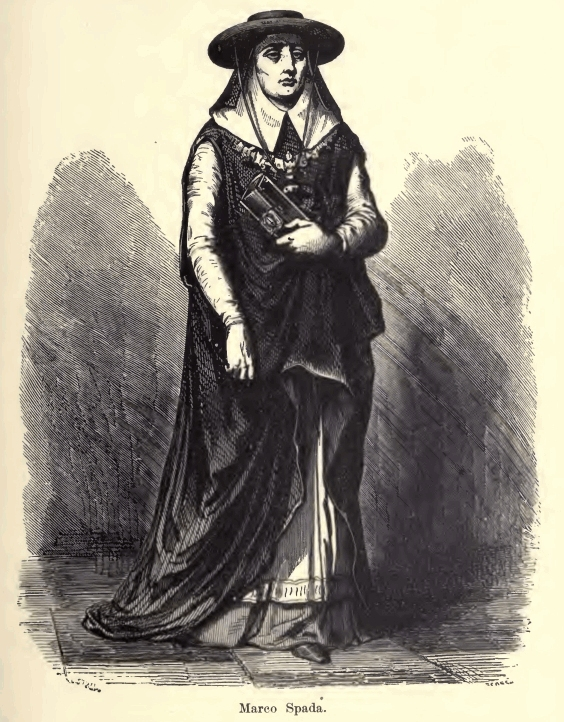
\includegraphics[width=\textwidth]{0239m.jpg}
\end{figure}

“It is time now to proceed to the last part of the speculation. The
pope heaped attentions upon Rospigliosi and Spada, conferred upon them
the insignia of the cardinalate, and induced them to arrange their
affairs and take up their residence at Rome. Then the pope and Cæsar
Borgia invited the two cardinals to dinner. This was a matter of
dispute between the Holy Father and his son. Cæsar thought they could
make use of one of the means which he always had ready for his friends,
that is to say, in the first place, the famous key which was given to
certain persons with the request that they go and open a designated
cupboard. This key was furnished with a small iron point,—a negligence
on the part of the locksmith. When this was pressed to effect the
opening of the cupboard, of which the lock was difficult, the person
was pricked by this small point, and died next day. Then there was the
ring with the lion’s head, which Cæsar wore when he wanted to greet his
friends with a clasp of the hand. The lion bit the hand thus favored,
and at the end of twenty-four hours, the bite was mortal.

“Cæsar proposed to his father, that they should either ask the
cardinals to open the cupboard, or shake hands with them; but Alexander
VI. replied: ‘Now as to the worthy cardinals, Spada and Rospigliosi,
let us ask both of them to dinner, something tells me that we shall get
that money back. Besides, you forget, Cæsar, an indigestion declares
itself immediately, while a prick or a bite occasions a delay of a day
or two.’ Cæsar gave way before such cogent reasoning, and the cardinals
were consequently invited to dinner.

“The table was laid in a vineyard belonging to the pope, near San
Pierdarena, a charming retreat which the cardinals knew very well by
report. Rospigliosi, quite set up with his new dignities, went with a
good appetite and his most ingratiating manner. Spada, a prudent man,
and greatly attached to his only nephew, a young captain of the highest
promise, took paper and pen, and made his will. He then sent word to
his nephew to wait for him near the vineyard; but it appeared the
servant did not find him.

“Spada knew what these invitations meant; since Christianity, so
eminently civilizing, had made progress in Rome, it was no longer a
centurion who came from the tyrant with a message, ‘Cæsar wills that
you die.’ but it was a legate \textit{à latere}, who came with a smile on his
lips to say from the pope, ‘His holiness requests you to dine with
him.’

“Spada set out about two o’clock to San Pierdarena. The pope awaited
him. The first sight that attracted the eyes of Spada was that of his
nephew, in full costume, and Cæsar Borgia paying him most marked
attentions. Spada turned pale, as Cæsar looked at him with an ironical
air, which proved that he had anticipated all, and that the snare was
well spread.

“They began dinner and Spada was only able to inquire of his nephew if
he had received his message. The nephew replied no; perfectly
comprehending the meaning of the question. It was too late, for he had
already drunk a glass of excellent wine, placed for him expressly by
the pope’s butler. Spada at the same moment saw another bottle approach
him, which he was pressed to taste. An hour afterwards a physician
declared they were both poisoned through eating mushrooms. Spada died
on the threshold of the vineyard; the nephew expired at his own door,
making signs which his wife could not comprehend.

“Then Cæsar and the pope hastened to lay hands on the heritage, under
pretense of seeking for the papers of the dead man. But the inheritance
consisted in this only, a scrap of paper on which Spada had written:—‘I
bequeath to my beloved nephew my coffers, my books, and, amongst
others, my breviary with the gold corners, which I beg he will preserve
in remembrance of his affectionate uncle.’

“The heirs sought everywhere, admired the breviary, laid hands on the
furniture, and were greatly astonished that Spada, the rich man, was
really the most miserable of uncles—no treasures—unless they were those
of science, contained in the library and laboratories. That was all.
Cæsar and his father searched, examined, scrutinized, but found
nothing, or at least very little; not exceeding a few thousand crowns
in plate, and about the same in ready money; but the nephew had time to
say to his wife before he expired: ‘Look well among my uncle’s papers;
there is a will.’

“They sought even more thoroughly than the august heirs had done, but
it was fruitless. There were two palaces and a vineyard behind the
Palatine Hill; but in these days landed property had not much value,
and the two palaces and the vineyard remained to the family since they
were beneath the rapacity of the pope and his son. Months and years
rolled on. Alexander VI. died, poisoned,—you know by what mistake.
Cæsar, poisoned at the same time, escaped by shedding his skin like a
snake; but the new skin was spotted by the poison till it looked like a
tiger’s. Then, compelled to quit Rome, he went and got himself
obscurely killed in a night skirmish, scarcely noticed in history.

“After the pope’s death and his son’s exile, it was supposed that the
Spada family would resume the splendid position they had held before
the cardinal’s time; but this was not the case. The Spadas remained in
doubtful ease, a mystery hung over this dark affair, and the public
rumor was, that Cæsar, a better politician than his father, had carried
off from the pope the fortune of the two cardinals. I say the two,
because Cardinal Rospigliosi, who had not taken any precaution, was
completely despoiled.

“Up to this point,” said Faria, interrupting the thread of his
narrative, “this seems to you very meaningless, no doubt, eh?”

“Oh, my friend,” cried Dantès, “on the contrary, it seems as if I were
reading a most interesting narrative; go on, I beg of you.”

“I will. The family began to get accustomed to their obscurity. Years
rolled on, and amongst the descendants some were soldiers, others
diplomatists; some churchmen, some bankers; some grew rich, and some
were ruined. I come now to the last of the family, whose secretary I
was—the Count of Spada. I had often heard him complain of the
disproportion of his rank with his fortune; and I advised him to invest
all he had in an annuity. He did so, and thus doubled his income. The
celebrated breviary remained in the family, and was in the count’s
possession. It had been handed down from father to son; for the
singular clause of the only will that had been found, had caused it to
be regarded as a genuine relic, preserved in the family with
superstitious veneration. It was an illuminated book, with beautiful
Gothic characters, and so weighty with gold, that a servant always
carried it before the cardinal on days of great solemnity.

“At the sight of papers of all sorts,—titles, contracts, parchments,
which were kept in the archives of the family, all descending from the
poisoned cardinal, I in my turn examined the immense bundles of
documents, like twenty servitors, stewards, secretaries before me; but
in spite of the most exhaustive researches, I found—nothing. Yet I had
read, I had even written a precise history of the Borgia family, for
the sole purpose of assuring myself whether any increase of fortune had
occurred to them on the death of the Cardinal Cæsar Spada; but could
only trace the acquisition of the property of the Cardinal Rospigliosi,
his companion in misfortune.

“I was then almost assured that the inheritance had neither profited
the Borgias nor the family, but had remained unpossessed like the
treasures of the Arabian Nights, which slept in the bosom of the earth
under the eyes of the genie. I searched, ransacked, counted, calculated
a thousand and a thousand times the income and expenditure of the
family for three hundred years. It was useless. I remained in my
ignorance, and the Count of Spada in his poverty.

“My patron died. He had reserved from his annuity his family papers,
his library, composed of five thousand volumes, and his famous
breviary. All these he bequeathed to me, with a thousand Roman crowns,
which he had in ready money, on condition that I would have anniversary
masses said for the repose of his soul, and that I would draw up a
genealogical tree and history of his house. All this I did
scrupulously. Be easy, my dear Edmond, we are near the conclusion.

“In 1807, a month before I was arrested, and a fortnight after the
death of the Count of Spada, on the 25th of December (you will see
presently how the date became fixed in my memory), I was reading, for
the thousandth time, the papers I was arranging, for the palace was
sold to a stranger, and I was going to leave Rome and settle at
Florence, intending to take with me twelve thousand francs I possessed,
my library, and the famous breviary, when, tired with my constant labor
at the same thing, and overcome by a heavy dinner I had eaten, my head
dropped on my hands, and I fell asleep about three o’clock in the
afternoon.

\begin{figure}[ht]
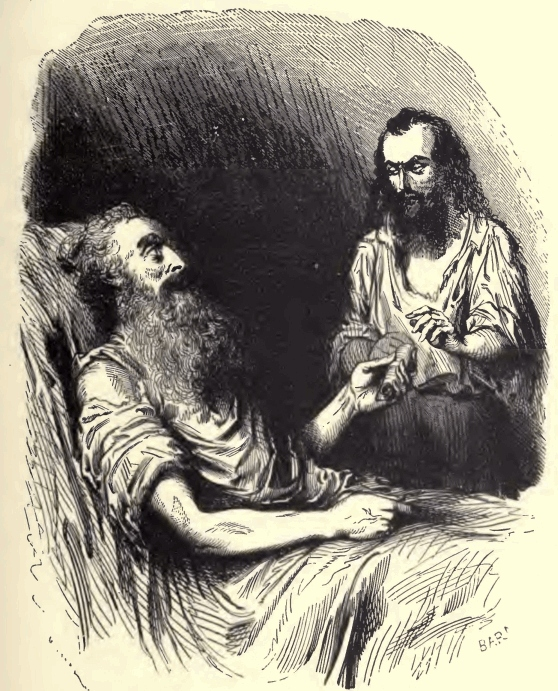
\includegraphics[width=\textwidth]{0243m.jpg}
\end{figure}

“I awoke as the clock was striking six. I raised my head; I was in
utter darkness. I rang for a light, but, as no one came, I determined
to find one for myself. It was indeed but anticipating the simple
manners which I should soon be under the necessity of adopting. I took
a wax-candle in one hand, and with the other groped about for a piece
of paper (my match-box being empty), with which I proposed to get a
light from the small flame still playing on the embers. Fearing,
however, to make use of any valuable piece of paper, I hesitated for a
moment, then recollected that I had seen in the famous breviary, which
was on the table beside me, an old paper quite yellow with age, and
which had served as a marker for centuries, kept there by the request
of the heirs. I felt for it, found it, twisted it up together, and
putting it into the expiring flame, set light to it.

“But beneath my fingers, as if by magic, in proportion as the fire
ascended, I saw yellowish characters appear on the paper. I grasped it
in my hand, put out the flame as quickly as I could, lighted my taper
in the fire itself, and opened the crumpled paper with inexpressible
emotion, recognizing, when I had done so, that these characters had
been traced in mysterious and sympathetic ink, only appearing when
exposed to the fire; nearly one-third of the paper had been consumed by
the flame. It was that paper you read this morning; read it again,
Dantès, and then I will complete for you the incomplete words and
unconnected sense.”

Faria, with an air of triumph, offered the paper to Dantès, who this
time read the following words, traced with an ink of a reddish color
resembling rust:

\vskip \onelineskip

\begin{quote}

{\small“This 25th day of April, 1498, be...

Alexander VI., and fearing that not...

he may desire to become my heir, and re...

and Bentivoglio, who were poisoned,...

my sole heir, that I have bu...

and has visited with me, that is, in...

Island of Monte Cristo, all I poss...

jewels, diamonds, gems; that I alone...

may amount to nearly two mil...

will find on raising the twentieth ro...

creek to the east in a right line. Two open...

in these caves; the treasure is in the furthest a...

which treasure I bequeath and leave en...

as my sole heir.

“25th April, 1498.

“Cæs...}
\end{quote}

\vskip \onelineskip

“And now,” said the abbé, “read this other paper;” and he presented to
Dantès a second leaf with fragments of lines written on it, which
Edmond read as follows:

\vskip \onelineskip

\begin{flushright}
{\small...ing invited to dine by his Holiness

...content with making me pay for my hat,

...serves for me the fate of Cardinals Caprara

...I declare to my nephew, Guido Spada

...ried in a place he knows

...the caves of the small

...essed of ingots, gold, money,

...know of the existence of this treasure, which

...lions of Roman crowns, and which he

...ck from the small

...ings have been made

...ngle in the second;

...tire to him

...ar † Spada.”}
\end{flushright}

\vskip \onelineskip

Faria followed him with an excited look.

“And now,” he said, when he saw that Dantès had read the last line,
“put the two fragments together, and judge for yourself.” Dantès
obeyed, and the conjointed pieces gave the following:

\begin{figure}[h]
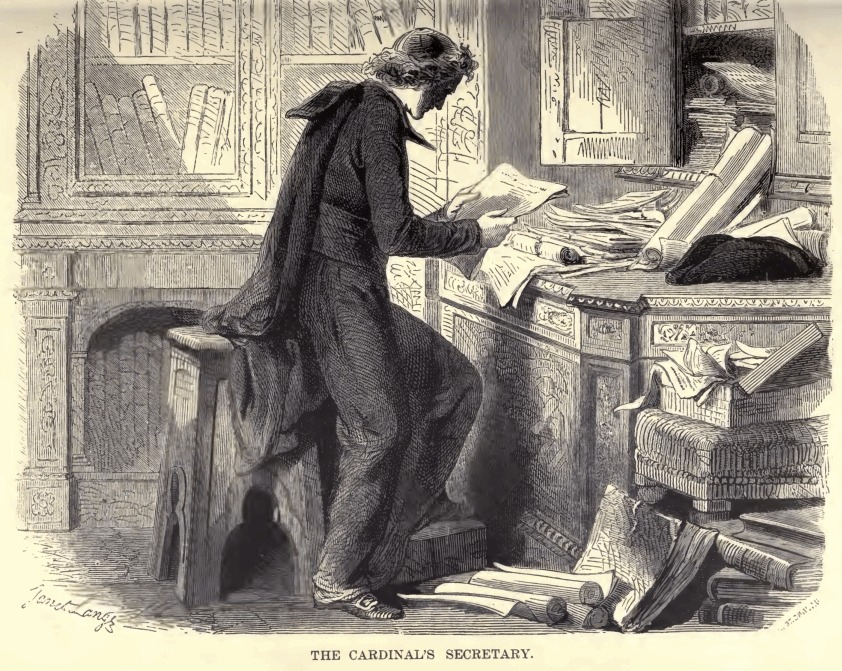
\includegraphics[width=\textwidth]{0245m.jpg}
\end{figure}

“This 25th day of April, 1498, be...ing invited to dine by his Holiness
Alexander VI., and fearing that not...content with making me pay for my
hat, he may desire to become my heir, and re...serves for me the fate
of Cardinals Caprara and Bentivoglio, who were poisoned,...I declare to
my nephew, Guido Spada, my sole heir, that I have bu...ried in a place
he knows and has visited with me, that is, in...the caves of the small
Island of Monte Cristo, all I poss...essed of ingots, gold, money,
jewels, diamonds, gems; that I alone...know of the existence of this
treasure, which may amount to nearly two mil...lions of Roman crowns,
and which he will find on raising the twentieth ro...ck from the small
creek to the east in a right line. Two open...ings have been made in
these caves; the treasure is in the furthest a...ngle in the second;
which treasure I bequeath and leave en...tire to him as my sole heir.
“25th April, 1498. “Cæs...ar † Spada.”

“Well, do you comprehend now?” inquired Faria.

“It is the declaration of Cardinal Spada, and the will so long sought
for,” replied Edmond, still incredulous.

“Yes; a thousand times, yes!”

“And who completed it as it now is?”

“I did. Aided by the remaining fragment, I guessed the rest; measuring
the length of the lines by those of the paper, and divining the hidden
meaning by means of what was in part revealed, as we are guided in a
cavern by the small ray of light above us.”

“And what did you do when you arrived at this conclusion?”

“I resolved to set out, and did set out at that very instant, carrying
with me the beginning of my great work, the unity of the Italian
kingdom; but for some time the imperial police (who at this period,
quite contrary to what Napoleon desired so soon as he had a son born to
him, wished for a partition of provinces) had their eyes on me; and my
hasty departure, the cause of which they were unable to guess, having
aroused their suspicions, I was arrested at the very moment I was
leaving Piombino.

“Now,” continued Faria, addressing Dantès with an almost paternal
expression, “now, my dear fellow, you know as much as I do myself. If
we ever escape together, half this treasure is yours; if I die here,
and you escape alone, the whole belongs to you.”

“But,” inquired Dantès hesitating, “has this treasure no more
legitimate possessor in the world than ourselves?”

“No, no, be easy on that score; the family is extinct. The last Count
of Spada, moreover, made me his heir, bequeathing to me this symbolic
breviary, he bequeathed to me all it contained; no, no, make your mind
satisfied on that point. If we lay hands on this fortune, we may enjoy
it without remorse.”

“And you say this treasure amounts to——”

“Two millions of Roman crowns; nearly thirteen millions of our money.”\footnote[2]{\$2,600,000
in 1894.}

“Impossible!” said Dantès, staggered at the enormous amount.

“Impossible? and why?” asked the old man. “The Spada family was one of
the oldest and most powerful families of the fifteenth century; and in
those times, when other opportunities for investment were wanting, such
accumulations of gold and jewels were by no means rare; there are at
this day Roman families perishing of hunger, though possessed of nearly
a million in diamonds and jewels, handed down by entail, and which they
cannot touch.”

Edmond thought he was in a dream—he wavered between incredulity and
joy.

“I have only kept this secret so long from you,” continued Faria, “that
I might test your character, and then surprise you. Had we escaped
before my attack of catalepsy, I should have conducted you to Monte
Cristo; now,” he added, with a sigh, “it is you who will conduct me
thither. Well, Dantès, you do not thank me?”

“This treasure belongs to you, my dear friend,” replied Dantès, “and to
you only. I have no right to it. I am no relation of yours.”

“You are my son, Dantès,” exclaimed the old man. “You are the child of
my captivity. My profession condemns me to celibacy. God has sent you
to me to console, at one and the same time, the man who could not be a
father, and the prisoner who could not get free.”

And Faria extended the arm of which alone the use remained to him to
the young man, who threw himself upon his neck and wept.

\chapter{TESTIMONY OF EARLY BRETHREN}

THE Tenth Article of Faith reads as follows:

"We believe in the literal gathering of Israel and in the restoration of the Ten Tribes; that
Zion will be built upon this [the American] continent; that Christ will reign personally upon
the earth; and, that the earth will be renewed and receive its paradisiacal glory."

We are also taught that we are living in the "Dispensation of the Fulness of Times." This is
the dispensation into which all other dispensations flow. It is spoken of in the scriptures as
"the times of restitution of all things, which God hath spoken by the mouth of all his holy
prophets since the world began." 1 If the earth is to be renewed, to what is it to be renewed?
It must be to some condition which prevailed in the beginning when the Lord pronounced it
"good." Isaiah, in the 65th chapter of his book gives us the story of what this restoration will
be. Likewise in the Doctrine and Covenants, Section 101, verses 23 to 30, we are given a
similar account, and in the same book, Section 133, the Lord reveals in some detail other
things pertaining to this restoration. This work of restoration commenced many years ago,
when the Lord prepared for the restoration of the Church in this dispensation, and received its
impetus when the Lord commenced his "marvelous work and a wonder." 2

We learn in Section 133, that the Ten Tribes are to come to the children of Ephraim to
receive their blessings and be restored; the Lamb shall come and stand on Mt. Zion, and on
the Mt. of Olives and "utter his voice out of Zion, and he shall speak from Jerusalem, and his
voice shall be heard among all people." His voice shall break down the mountains, the "great
deep" shall be driven \textit{back} into the North countries, and the islands shall become one land
and Jerusalem and Zion shall be turned back to their own place, "and the earth shall be like as
it was in the days before it was divided. And the Lord, even the Savior, shall stand in the
midst of his people, and shall reign over all flesh."

Some of our brethren who lived in the days of the Prophet Joseph Smith have written
interesting accounts of this condition which was in the beginning and what it will be like in
the restoration. First we will present parts of the story as related by Elder Parley P. Pratt, in
his \textit{Voice of Warning} and as it is re-published by John Taylor, in his \textit{The Government of God.}
President Taylor introduces the quotation from Elder Parley P. Pratt's writings with the
following sentence:

Now, restoration signifies a bringing back, and must refer to something which existed before;
for if it did not exist before, it could not be restored. I cannot describe this better than Parley
P. Pratt has done in his \textit{Voice of Warning}, and shall therefore make the following extract:—. .
.

Now, we can never understand precisely what is meant by restoration, unless we understand
what is lost or taken away; for instance, when we offer to restore any thing to a man, it is as
much as to say he once possessed it, but had lost it, and we propose to replace or put him in
possession of that which he once had; therefore, when a prophet speaks of the restoration of
\textit{all things}, he means \textit{all things} have undergone a change, and are to be again restored to their
primitive order even as they first existed.

First, then, it becomes necessary for us to take a view of creation as it rolled in purity from
the hand of its Creator; and if we can discover the true state in which it then existed, and
understand the changes that have taken place since, then we shall be able to understand what
is to be restored; and thus our minds being prepared, we shall be looking for the very things
which will come, and shall be in no danger of lifting our puny arm, in ignorance, to oppose
the things of God.

First, then, we will take a view of the earth, as to its surface, local situation, and productions.

When God had created the heavens and the earth, and separated the light from the darkness,
his next command was to the waters, Gen. 1:9—And God said, "Let the waters under the
heaven be gathered together into \textit{one place}, and let the dry land appear: and it was so!" From
this we learn a marvelous fact, which very few ever realized or believed in this benighted
age; we learn that the waters, which are now divided into oceans, seas, and lakes, were then
all gathered together, into one vast ocean; and, consequently, that the land, which is now torn
asunder, and divided into continents and islands, almost innumerable, was then \textit{one} vast
continent or body, \textit{not} separated as it is now.

Second, we hear the Lord God pronounce the earth, as well as every thing else, \textit{very good.}
From this we learn that there were neither deserts, barren places, stagnant swamps, rough,
broken, ragged hills, nor vast mountains covered with eternal snows; and no part of it was
located in the frigid zones, so as to render its climate dreary and unproductive, subject to
eternal frost, or everlasting chains of ice,—

Where no sweet flowers the dreary landscape cheer, Nor plenteous harvests crown the
passing year;

but the whole earth was probably one vast plain, or interspersed with gently rising hills, and
sloping vales, well calculated for cultivation; while its climate was delightfully varied with
the moderate changes of heat and cold, of wet and dry, which only tended to crown the
varied year, with the greater variety of productions, all for the good of man, animal, fowl, or
creeping thing; while from the flowery plain, or spicy grove, sweet odors were wafted on
every breeze; and all the vast creation of animated beings breathed naught but health, peace,
and joy.

Next, we learn from Genesis 1:29-30, "And God said, Behold, I have given you every herb
bearing seed, which is upon the face of all the earth, and every tree, in which is the fruit of a
tree, yielding seed; to you it shall be for meat. And to every beast of the earth, and to every
fowl of the air, and to every thing that creepeth upon the earth, wherein there is life, I have
given every green herb for meat: and it was so." From these verses we learn that the earth
yielded neither noxious weeds nor poisonous plants, nor useless thorns and thistles; indeed,
everything that grew was just calculated for the food of man, beast, fowl, and creeping thing;
and their food was all vegetable; flesh and blood were never sacrificed to glut their souls, or
gratify their appetites; the beasts of the earth were all in perfect harmony with each other; the
lion ate straw like the ox—the wolf dwelt with the lamb—the leopard lay down with the
kid—the cow and bear fed together, in the same pasture . . . in perfect security, under the
shade of the same trees; all was peace and harmony, and nothing to hurt nor disturb, in all the
holy mountain.

And to crown the whole, we behold man created in the image of God, and exalted in dignity
and power, having dominion over all the vast creation of animated beings, which swarmed
through the earth, while at the same time, he inhabits a beautiful and well-watered garden, in
the midst of which stood the tree of life, to which he had free access; while he stood in the
presence of his Maker, conversed with him face to face, and gazed upon his glory, without a
dimming veil between. O reader, contemplate, for a moment, this beautiful creation, clothed
with peace and plenty; the earth teeming with harmless animals, rejoicing over all the plain,
the air swarming with delightful birds, whose never ceasing notes filled the air with varied
melody; and all in subjection to their rightful sovereign who rejoiced over them; while, in a
delightful garden—the capital of creation,—man was seated on the throne of his vast empire,
swaying his scepter over all the earth, with undisputed right; while legions of angels
encamped round about him, and joined their glad voices in grateful songs of praise, and
shouts of joy; neither a sign nor a groan was heard, throughout the vast expanse; neither was
there sorrow, tears, pain, weeping, sickness, nor death; neither contention, wars, nor
bloodshed; but peace crowned the seasons as they rolled, and life, joy, and love reigned over
all his works. But, O! how changed the scene.

It now becomes my painful duty, to trace some of the important changes, which have taken
place, and the causes which have conspired to reduce the earth and its inhabitants to their
present state.

First, man fell from his standing before God, by giving heed to temptation; and this fall
affected the whole creation, as well as man, and caused various changes to take place; he was
banished from the presence of his Creator, and a veil was drawn between them, and he was
driven from the garden of Eden, to till the earth, which was cursed for man's sake, and should
bring forth thorns and thistles; and in the sweat of his face should earn his bread, and in
sorrow eat of it, all the days of his life, and finally return to dust. But as to Eve, her curse was
a great multiplicity of sorrow and conception; and between her and the seed of the serpent,
there was to be a constant enmity; it should bruise the serpent's head, and the serpent should
bruise his heel.

Now, reader, contemplate the change. This scene, which was so beautiful a little while
before, had now become the abode of sorrow and toil, of death and mourning; the earth
groaned with its production of accursed thorns and thistles; man and beast at enmity; the
serpent slily creeping away, fearing lest his head should get the deadly bruise; and man
starting amid the thorny path, in fear, lest the serpent's fangs should pierce his heel; while the
lamb yields his blood upon the smoking altar. Soon man begins to persecute, hate, and
murder his fellow; until at length the earth is filled with violence; all flesh becomes corrupt,
the powers of darkness prevail; and it repented Noah that God had made man, and it grieved
him at his heart, because the Lord should come out in vengeance, and cleanse the earth by
water.

How far the flood may have contributed, to produce the various changes, as to the division of
the earth into broken fragments, islands and continents, mountains and valleys, we have not
been informed; the change must have been considerable. But after the flood, in the days of
Peleg, the earth was divided.—See Gen. 10:25,—a short history, to be sure, of so great anevent; but still it will account for the mighty revolution, which rolled the sea from its own
place in the north, and brought it to interpose between different portions of the earth, which
were thus parted asunder, and moved into something near their present form; this, together
with the earthquakes, revolutions, and commotions which have since taken place, have all
contributed to reduce the face of the earth to its present state; while the great curses which
have fallen upon different portions, because of the wickedness of men, will account for the
the stagnant swamps, the sunken lakes, the dead seas, and great deserts.

Then speaking of the restoration we have a continuation as follows:

Thus you see, every mountain being laid low, and every valley exalted, and the rough places
being made plain, and the crooked straight, that these mighty revolutions will begin to restore
the face of the earth to its former beauty. But all this done, we have not yet gone through our
restoration; there are many more great things to be done, in order to restore all things. . . .

Thus, having cleansed the earth, and glorified it with the knowledge of God, as the waters
cover the sea, and having poured out his Spirit upon all flesh, both men and beast becoming
perfectly harmless, as they were in the beginning, and feeding on vegetable food only, while
nothing is left to hurt or destroy in all the vast creation, the prophets then proceed to give us
many glorious descriptions of the enjoyment of its inhabitants. "They shall build houses and
inhabit them; they shall plant vineyards, and drink the wine of them; they shall plant gardens
and eat the fruit of them; they shall not build and another inhabit; they shall not plant and
another eat; for as the days of a tree are the days of my people, and mine elect shall enjoy the
work of their hands. They shall not labor in vain, nor bring forth in trouble; for they are the
seed of the blessed of the Lord, and their offspring with them; and it shall come to pass, that
before they call I will answer, and while they are yet speaking I will hear." In this happy state
of existence it seems that all people will live to the full age of a tree, and this too without
pain or sorrow, and whatsoever they ask will be immediately answered, and even all their
wants will be anticipated. Of course, then, none of them will sleep in the dust, for they will
prefer to be translated; that is, changed in the twinkling of an eye, from mortal to immortal;
after which they will continue to reign with Jesus on the earth.

A great council will then be held to adjust the affairs of the world, from the commencement,
over which Father Adam will preside as head and representative of the human family. There
have been, in different ages of the world, communications opened between the heavens and
the earth. (\textit{Voice of Warning and Government of God}, pages 106-115.)

TESTIMONY OF ORSON PRATT

At the funeral of Caroline Grant Smith, wife of William B. Smith, in Nauvoo, May 24, 1845,
Elder Orson Pratt gave the following in his discourse:

In the morning of creation all things were pronounced good by the Creator, as they rolled
into organized existence unsullied and without a curse. Man, the last and noblest of God's
creations, was placed in the garden of Eden, being governed by laws and restricted by
commandments, not being subject to sickness, disease, or death. Adam was placed upon the
earth an immortal being. He was placed in the garden to dress, beautify and adorn it, and to
hold the supremacy of power over all the things of God's creation.

Instead of our first parents eating animal food, they subsisted upon herbs and the fruits of the
earth, which were originally designed for the food of man, and had they not transgressed they
would have both been living upon the earth at the present day, as fair, as healthy, as beautiful
and as free from sickness and death, as they were previous to the transgression. What was
that transgression? it was violating a single commandment of God, and disregarding the
counsel of those immortal beings who stood above them in authority. . . . His was a simple
commandment; but the violation of it subjected Adam to the fall from his exalted station in
the favor of God. Consequently a curse was placed upon all created things, and in the
posterity of Adam were sown the seeds of dissolution. . . . That transgression subjected him
to a curse and that was a fall from a state of immortality to that of mortality; consequently
you see that it was through his agency that death entered the world. (\textit{Times and Seasons}, Vol.
6, pp. 918-919.)

August 29, 1852, the First Presidency asked Orson Pratt to give a discourse on marriage. In
this discourse Elder Pratt said:

The Lord himself solemnized the first marriage pertaining to this globe, and pertaining to
flesh and bones here upon this earth. I do not say pertaining to mortality; for when the first
marriage was celebrated, no mortality was here. The first marriage that we have any account
of, was between two immortal beings—old father Adam and old mother Eve; they were
immortal beings: death had no dominion nor power over them; and they were capable of
enduring forever and ever in their organization. . . .

What would you consider, my hearers, if a marriage was to be celebrated between beings not
subject to death? Would you consider them joined together for a certain number of years, and
that then all their covenants were to cease for ever, and the marriage contract to be dissolved?
Would it look reasonable and consistent? Every heart would say that the work of God is
perfect in and of itself, and inasmuch as sin had not brought imperfection upon the globe,
what God joined together could not be dissolved, and destroyed and torn asunder by any
power beneath the celestial world, consequently it was eternal; the sealing of the great
Jehovah upon Adam and Eve was eternal in its nature. (\textit{Journal of Discourses} Vol. 1, p. 58.)

Again, July 25, 1852, Elder Orson Pratt preached a wonderful discourse, designated as "A
funeral sermon of all Saints and Sinners; also of the heavens and the Earth." This entire
discourse which is printed in the Millennial Star and other publications, should be read by
every member of the Church. It cannot be produced here in its fulness, but the following
taken from it has to do with the subject of Adam and the fall.

I will take a text, which you will find recorded in the 51st chapter of the prophecy of Isaiah,
and the sixth verse: "Lift up your eyes to the heavens, and look upon the earth beneath: for
the heavens shall vanish away like smoke, and the earth shall wax old like a garment, and
they that dwell therein shall die in like manner: but my salvation shall be forever, and my
righteousness shall not be abolished!"

All things with which we are acquainted, pertaining to this earth of ours, are subject to
change; not only man, so far as his temporal body is concerned, but the beasts of the field,
the fowls of the air, the fishes of the sea, and every living thing with which we are
acquainted—all are subject to pain and distress, and finally die and pass away; death seems
to have universal dominion in our creation. It certainly is a curious world; it certainly does
not look like a world constructed in such manner as to produce eternal happiness; and it
would be very far from the truth, I think, for any being at the present time to pronounce it
very good; everything seems to show us that goodness, in a great degree, has fled from this
creation. If we partake of the elements, death is there in all its forms and varieties; and when
we desire to rejoice, sorrow is there, mingling itself in every cup; and woe, and
wretchedness, and misery, seem to be our present doom.

There is something, however, in man, that is constantly reaching forward after happiness,
after pleasure, after something to satisfy the longing desire that dwells within his bosom.
Why is it that we have such a desire? And why is it that it is not satisfied? Why is it that this
creation is so constructed? And why is it that death reigns universally over all living earthly
beings? Did the great Author of creation construct this little globe of ours subject to all these
changes, which are calculated to produce sorrow and death among the beings that inhabit it?
Was this the original condition of our creation? I answer, no; it was not so constructed. But
how was it made in the beginning? All things that were made pertaining to this earth were
pronounced "very good." Where there is pain, where there is sickness, where there is sorrow,
and where there is death, this saying can not be understood in its literal sense; things cannot
be very good where something very evil reigns and has universal dominion.

We are, therefore, constrained to believe, that in the first formation of our globe, as far as the
Mosaic history gives us the information, everything was perfect in its formation; that there
was nothing in the air, or in the waters or in the solid elements that was calculated to produce
misery, wretchedness, unhappiness, or death, in the way that it was then organized; not but
what the same elements, organized a little differently, would produce all these effects; but as
it was then constructed, we must admit that every particle of air, of water, and earth, was so
organized as to be capable of diffusing life and immortality through all the varied species of
animated existence—immortality reigned in every department of creation; hence it was
pronounced "very good."

When the Lord made the fowls of the air, and the fishes of the sea, to people the atmospheric
heavens, or the watery elements, these fowls and fishes were so constructed in their nature as
to be capable of eternal existence. To imagine anything different from this, would be to
suppose the Almighty to form that which was calculated to produce wretchedness and
misery. What says the Psalmist David upon the subject? He says that all the works of the
Lord shall endure forever. Did not the Lord make the fish? Did he not make the fowls of the
heavens? Yes. Did he not make the beasts of the field, and the creeping things, and the
insects? Yes. Do they endure forever? They apparently do not; and yet David says all his
works are constructed upon that principle. Is this a contradiction? No. God has given some
other particulars in relation to these works. He has permitted the destroyer to visit them, who
has usurped a certain dominion and authority, carrying desolation and ruin on every hand; the
perfections of the original organizations have ceased. But will the Lord for ever permit these
destructions to reign? No. His power exists, and the power of the destroyer exists. His power
exists, and the power of death exists; but his power exceeds all other powers; and
consequently wherever a usurper comes in and lays waste any of his works, he will repair
these wastes, build up the old ruins, and make all things new: Even the fish of the sea, and
the fowls of the heavens, and the beasts of the earth, must yet, in order to carry out the
designs of the Almighty, be so constructed as to be capable of eternal existence.

It would be interesting to know something about the situation of things when they were first
formed, and how this destroyer happened to make inroads upon this fair creation; what the
causes were, and why it was permitted.

Man, when he was first placed upon this earth, was an immortal being, capable of eternal
endurance; his flesh and bones, as well as his spirit, were immortal and eternal in their
nature; and it was just so with all the inferior creation—the lion, the leopard, the kid, and the
cow; it was so with the feathered tribes of creation, as well as those that swim in the vast
ocean of waters; all were immortal and eternal in their nature; and the earth itself, as a living
being, was immortal and eternal in its nature. What! is the earth alive too? If it were not, how
could the words of our text be fulfilled, where it speaks of the earth's dying? How can that
die that has no life? "Lift up your eyes to the heavens above, say the Lord, and look upon the
earth beneath: for the heavens shall vanish away like smoke, and the earth shall wax old like
a garment, and they that dwell therein shall die in like manner." What! the earth and the
heavens to die? Yes, the material heavens and the earth must all undergo this change which
we call death; and if so, the earth must be alive as well as we. The earth was so constructed
that it was capable of existing as a living being to all eternity, with all the swarms of animals,
fowls, and fishes that were first placed upon the face thereof. But how can it be proved that
man was an immortal being? We will refer you to what the Apostle Paul has written upon
this subject: he says that by one man came death; and he tells us how it came: It was by the
transgression of one individual that death was introduced here. But did transgression bring in
all these diseases and this sorrow, this misery and wretchedness, over the whole face of this
creation? Is it by the transgression of one person that the very heavens are to vanish away as
smoke, and the earth is to wax old like a garment? Yes, it is by the transgression of one; and
if it had not been for his transgression, the earth never would have been subject to death.
Why? Because the works of the Lord are so constructed as to exist for ever; and if death had
come in without a cause, and destroyed the earth, and laid waste the material heavens, and
produced a general and utter overthrow and ruin in this fair creation, then the works of the
Lord would have ceased to endure according to the promise, being imperfect in their
construction, and consequently not very good.

But what was the sin, and what was the nature of it? I will tell you what it was; it was merely
the partaking of a certain kind of fruit. But, says one, "I should think there is no harm in
eating fruit." There would not be unless God gave a command upon the subject. There are
things in nature that would be evil without a commandment: If there were no commandment,
it would be evil for you to murder an innocent being, and your own conscience would tell
you it was an evil thing. It is an evil for any individual to injure another, or to infringe upon
the rights of another, independent of any revealed law; for the savage, or that being who has
never heard of the written laws of heaven—who has never heard of the revealed laws of
God—with regard to these principles—as well as the Saint, knows that it is an evil to infringe
upon the rights of another; the very nature of the thing shows that it is an evil; but not so in
regard to many other things that are evil; which are only made evil by commandment.

For instance, here is the Sabbath day; a person who never heard the revealed law of God
upon the subject, never could conceive that it was an evil to work on the Sabbath day; he
would consider it just as right to work on the first day of the week, as on the seventh; he
would perceive nothing in the nature of the thing by which he could distinguish it to be an
evil. So with regard to eating certain fruit, it was the commandment of the Great God that
made it an evil. He said to Adam and Eve, "Here are all the fruits of the garden; you may eat
of them freely except this one tree that stands in the midst of the garden; now beware for in
the day you eat thereof you shall surely die." Don't we perceive that the commandment made
this an evil? Had it not been for this commandment, Adam would have walked forth and
freely partaken of every tree, without any remorse of conscience; just as the savage, who
never had heard the revealed will of God, would work on the Sabbath, the same as on any
other day, and have no conscience about the matter. But when a man murders, he knows it to
be an injury, and he has a conscience about it, though he never heard of God; and so with
thousands of evils. But why did the Lord place man under these peculiar circumstances?
Why did he not withhold the commandment, if the partaking of the fruit, after the
commandment was given, was sin? Why should there have been a commandment upon the
subject at all, inasmuch as there was no evil in the nature of the thing to be perceived or
understood? The Lord had a purpose in view; though he constructed this fair creation, as we
have told you, subject to immortality, and capable of eternal endurance, and though he had
constructed men capable of living forever, yet he had an object in view in regard to that man,
and the creation he inhabited. What was the object? And when shall this object be
accomplished?

Why, the Lord wanted this intelligent being called man, to prove himself; inasmuch as he
was an agent. He desired that he should show himself approved before his Creator.

How could this be done without a commandment? Can you devise any possible means? Is
there any person in this congregation having wisdom sufficient to devise any means by which
an intelligent being can show himself approved before a superior intelligence, unless it be by
administering to that man certain laws to be kept? No. Without law, without commandment
or rule, there could be no possible way of showing his integrity; it could not be said that he
would keep all the laws that govern superior orders of beings, unless he had been placed in a
position to be tried, and thus proved whether he would keep them or not. Then it was wisdom
to try the man and the woman, so the Lord gave them this commandment; if he had not
intended the man should be tried by this commandment, he never would have planted that
tree. He never would have placed it in the midst of the garden. Now the very fact that he
planted it where the man could have easy access to it, shows that he intended man should be
tried by it, and thus prove whether he would keep his commandments or not. The penalty of
disobedience to this law was death.

But could he not give a commandment, without affixing a penalty? He could not; it would be
folly, even worse than folly, for God to give a law to an intelligent being, without affixing a
penalty to it if it were broken. Why? Because all intelligent beings would discard the very
idea of a law being given, which might be broken at pleasure, without the individuals
breaking it being punished for their transgression. They would say—"Where is the principle
of justice in the giver of the law? It is not here: we do not reverence him nor his law; justice
does not have an existence in his bosom. He does not regard his own laws, for he suffers
them to be broken with impunity, and trampled under foot by those whom he has made;
therefore we care not for him or his laws; nor his pretended justice. We will rebel against it.
Where would have been the use of it if there had been no penalty affixed?

But what is the nature of this penalty? It was wisely ordained to be of such a nature as to
instruct man. Penalties inflicted upon human beings here, by governors, kings, or rulers, are
generally of such a nature as to benefit them.

Adam was appointed lord of this creation; a great governor, swaying the scepter of power
over the whole earth. When the governor, the person who was placed to reign over this fair
creation, had transgressed, all in his dominion had to feel the effects of it, the same as a
father or a mother, who transgress certain laws, frequently transmit the effects thereof to the
latest generations.

How often do we see certain diseases becoming hereditary, being handed down from father
to son for generations? Why? Because in the first instance there was a transgression, and the
children partook of the effects of it. And what was the fullest extent of the penalty of Adam's
transgression? I will tell you—it was death. The death of the immortal tabernacle—of the
tabernacle where the seeds of death had not been, that was wisely framed, and pronounced
very good; the seeds of death were introduced into it. How and in what manner? Some say
there was something in the nature of the fruit that introduced mortality. Be this as it may, one
thing is certain, death entered into the system; it came there by some means, and sin was the
main spring by which this monster was introduced. If there had been no sin, our father Adam
would at this day have been in the garden of Eden, as bright and as blooming, as fresh and as
fair, as ever, together with his lovely consort Eve, dwelling in all the beauty of youth.

By one man came death—the death of the body. What becomes of the spirit when the body
dies? Will it be perfectly happy? Would old father Adam's spirit have gone back into the
presence of God, and dwelt there eternally, enjoying all the felicities and glories of heaven,
after his body had died? No; for the penalty of that transgression was not limited to the body
alone. When he sinned, it was with both the body and the spirit that he sinned. It was not only
the body that ate of the fruit, but the spirit gave the will to eat; the spirit sinned therefore as
well as the body; they were agreed in partaking of that fruit. Was not the spirit to suffer then
as well as the body? Yes. How long? To all ages of eternity, without any end, while the body
was to return back to its mother earth, and there slumber to all eternity. That was the effect of
the fall, leaving out the plan of redemption; so that, if there had been no plan of redemption
prepared from before the foundation of the world, man would have been subject to an eternal
dissolution of the body and spirit—the one to lie mingling with its mother earth, to all ages of
eternity, and the other to be subject, throughout all future duration, to the power that deceived
him, and led them astray; to be completely miserable, or as the Book of Mormon says, "dead
as to things pertaining to righteousness." (\textit{Journal of Discourses}, Vol. 1, pp. 280-284.)

From an epistle by the Prophet to the Elders in Missouri, sent January 22, 1834, the
following is taken:

Though man in his own supposed wisdom would not admit the influence of a power superior
to his own, yet for wise and great purposes, for the good and happiness of his creatures, God
has instructed man to form wise and wholesome laws, since he had departed from him and
refused to be governed by those laws which God had given by his own voice from on high in
the beginning. But notwithstanding the transgression, by which man had cut himself off from
an immediate intercourse with his maker without a Mediator, it appears that the great and
glorious plan of his redemption was previously provided: the sacrifice prepared; the
atonement wrought out in the mind and purpose of God, even in the person of the Son,
through whom man was now to look for acceptance and through whose merits he was now
taught that he alone could find redemption, since the word had been pronounced, Unto dust
thou shalt return.

But that man was not able himself to erect a system, or plan with power sufficient to free him
from a destruction which awaited him is evident from the fact that God, as before remarked,
prepared a sacrifice in the gift of his own Son who should be sent in due time, to prepare a
way, or open a door through which man might enter into the Lord's presence, whence he had
been cast out for disobedience. From time to time these glad tidings were sounded in the ears
of men in different ages of the world down to the time of Messiah's coming. By faith in the
atonement or plan of redemption, Abel offered to God a sacrifice that was accepted, which
was the firstlings of the flock. Cain offered of the fruit of the ground, and was not accepted,
because he could not do it in faith; he could have no faith, or could not exercise faith contrary
to the plan of heaven. It must be shedding of blood of the Only Begotten to atone for man;
for this was the plan of redemption; and without the shedding of blood was no remission; and
as the sacrifice was instituted as a type, by which man was to discern the great Sacrifice
which God had prepared; to offer a sacrifice contrary to that, no faith could be exercised,
because redemption was not purchased in that way, nor the power of atonement instituted
after that order; consequently Cain could have no faith; and whatsoever is not faith is sin.
(\textit{Teachings of the Prophet Joseph Smith}, pp. 57-58.)

\newpage
Footnotes

1. Acts 3:21.

2. D. \& C. Sec. 4.


\chapter{Conversion Of Constantine.}
\section{Part \thesection.}

\textit{The Motives, Progress, And Effects Of The Conversion Of
Constantine. — Legal Establishment And Constitution Of The Christian Or
Catholic Church.}
\vspace{\onelineskip}

The public establishment of Christianity may be considered as one of
those important and domestic revolutions which excite the most lively
curiosity, and afford the most valuable instruction. The victories and
the civil policy of Constantine no longer influence the state of
Europe; but a considerable portion of the globe still retains the
impression which it received from the conversion of that monarch; and
the ecclesiastical institutions of his reign are still connected, by an
indissoluble chain, with the opinions, the passions, and the interests
of the present generation. In the consideration of a subject which may
be examined with impartiality, but cannot be viewed with indifference,
a difficulty immediately arises of a very unexpected nature; that of
ascertaining the real and precise date of the conversion of
Constantine. The eloquent Lactantius, in the midst of his court, seems
impatient\textsuperscript{1} to proclaim to the world the glorious example of the
sovereign of Gaul; who, in the first moments of his reign, acknowledged
and adored the majesty of the true and only God.\textsuperscript{2} The learned Eusebius
has ascribed the faith of Constantine to the miraculous sign which was
displayed in the heavens whilst he meditated and prepared the Italian
expedition.\textsuperscript{3} The historian Zosimus maliciously asserts, that the
emperor had imbrued his hands in the blood of his eldest son, before he
publicly renounced the gods of Rome and of his ancestors.\textsuperscript{4} The
perplexity produced by these discordant authorities is derived from the
behavior of Constantine himself. According to the strictness of
ecclesiastical language, the first of the \textit{Christian} emperors was
unworthy of that name, till the moment of his death; since it was only
during his last illness that he received, as a catechumen, the
imposition of hands,\textsuperscript{5} and was afterwards admitted, by the initiatory
rites of baptism, into the number of the faithful.\textsuperscript{6} The Christianity
of Constantine must be allowed in a much more vague and qualified
sense; and the nicest accuracy is required in tracing the slow and
almost imperceptible gradations by which the monarch declared himself
the protector, and at length the proselyte, of the church. It was an
arduous task to eradicate the habits and prejudices of his education,
to acknowledge the divine power of Christ, and to understand that the
truth of \textit{his} revelation was incompatible with the worship of the
gods. The obstacles which he had probably experienced in his own mind,
instructed him to proceed with caution in the momentous change of a
national religion; and he insensibly discovered his new opinions, as
far as he could enforce them with safety and with effect. During the
whole course of his reign, the stream of Christianity flowed with a
gentle, though accelerated, motion: but its general direction was
sometimes checked, and sometimes diverted, by the accidental
circumstances of the times, and by the prudence, or possibly by the
caprice, of the monarch. His ministers were permitted to signify the
intentions of their master in the various language which was best
adapted to their respective principles;\textsuperscript{7} and he artfully balanced the
hopes and fears of his subjects, by publishing in the same year two
edicts; the first of which enjoined the solemn observance of Sunday,\textsuperscript{8}
and the second directed the regular consultation of the Aruspices.\textsuperscript{9}
While this important revolution yet remained in suspense, the
Christians and the Pagans watched the conduct of their sovereign with
the same anxiety, but with very opposite sentiments. The former were
prompted by every motive of zeal, as well as vanity, to exaggerate the
marks of his favor, and the evidences of his faith. The latter, till
their just apprehensions were changed into despair and resentment,
attempted to conceal from the world, and from themselves, that the gods
of Rome could no longer reckon the emperor in the number of their
votaries. The same passions and prejudices have engaged the partial
writers of the times to connect the public profession of Christianity
with the most glorious or the most ignominious æra of the reign of
Constantine.

\pagenote[1]{The date of the Divine Institutions of Lactantius has been
accurately discussed, difficulties have been started, solutions
proposed, and an expedient imagined of two \textit{original} editions; the
former published during the persecution of Diocletian, the latter under
that of Licinius. See Dufresnoy, Prefat. p. v. Tillemont, Mém.
Ecclesiast. tom. vi. p. 465-470. Lardner’s Credibility, part ii. vol.
vii. p. 78-86. For my own part, I am \textit{almost} convinced that Lactantius
dedicated his Institutions to the sovereign of Gaul, at a time when
Galerius, Maximin, and even Licinius, persecuted the Christians; that
is, between the years 306 and 311.}

\pagenote[2]{Lactant. Divin. Instit. i. l. vii. 27. The first and most
important of these passages is indeed wanting in twenty-eight
manuscripts; but it is found in nineteen. If we weigh the comparative
value of these manuscripts, one of 900 years old, in the king of
France’s library may be alleged in its favor; but the passage is
omitted in the correct manuscript of Bologna, which the P. de
Montfaucon ascribes to the sixth or seventh century (Diarium Italic. p.
489.) The taste of most of the editors (except Isæus; see Lactant.
edit. Dufresnoy, tom. i. p. 596) has felt the genuine style of
Lactantius.}

\pagenote[3]{Euseb. in Vit. Constant. l. i. c. 27-32.}

\pagenote[4]{Zosimus, l. ii. p. 104.}

\pagenote[5]{That rite was \textit{always} used in making a catechumen, (see
Bingham’s Antiquities. l. x. c. i. p. 419. Dom Chardon, Hist. des
Sacramens, tom. i. p. 62,) and Constantine received it for the \textit{first}
time (Euseb. in Vit Constant. l. iv. c. 61) immediately before his
baptism and death. From the connection of these two facts, Valesius (ad
loc. Euseb.) has drawn the conclusion which is reluctantly admitted by
Tillemont, (Hist. des Empereurs, tom. iv. p. 628,) and opposed with
feeble arguments by Mosheim, (p. 968.)}

\pagenote[6]{Euseb. in Vit. Constant. l. iv. c. 61, 62, 63. The legend
of Constantine’s baptism at Rome, thirteen years before his death, was
invented in the eighth century, as a proper motive for his \textit{donation}.
Such has been the gradual progress of knowledge, that a story, of which
Cardinal Baronius (Annual Ecclesiast. A. D. 324, No. 43-49) declared
himself the unblushing advocate, is now feebly supported, even within
the verge of the Vatican. See the Antiquitates Christianæ, tom. ii. p.
232; a work published with six approbations at Rome, in the year 1751
by Father Mamachi, a learned Dominican.}

\pagenote[7]{The quæstor, or secretary, who composed the law of the
Theodosian Code, makes his master say with indifference, “hominibus
supradictæ religionis,” (l. xvi. tit. ii. leg. 1.) The minister of
ecclesiastical affairs was allowed a more devout and respectful style,
[**Greek] the legal, most holy, and Catholic worship.}

\pagenote[8]{Cod. Theodos. l. ii. viii. tit. leg. 1. Cod. Justinian. l.
iii. tit. xii. leg. 3. Constantine styles the Lord’s day \textit{dies solis},
a name which could not offend the ears of his pagan subjects.}

\pagenote[9]{Cod. Theodos. l. xvi. tit. x. leg. l. Godefroy, in the
character of a commentator, endeavors (tom. vi. p. 257) to excuse
Constantine; but the more zealous Baronius (Annal. Eccles. A. D. 321,
No. 17) censures his profane conduct with truth and asperity.}

Whatever symptoms of Christian piety might transpire in the discourses
or actions of Constantine, he persevered till he was near forty years
of age in the practice of the established religion;\textsuperscript{10} and the same
conduct which in the court of Nicomedia might be imputed to his fear,
could be ascribed only to the inclination or policy of the sovereign of
Gaul. His liberality restored and enriched the temples of the gods; the
medals which issued from his Imperial mint are impressed with the
figures and attributes of Jupiter and Apollo, of Mars and Hercules; and
his filial piety increased the council of Olympus by the solemn
apotheosis of his father Constantius.\textsuperscript{11} But the devotion of
Constantine was more peculiarly directed to the genius of the Sun, the
Apollo of Greek and Roman mythology; and he was pleased to be
represented with the symbols of the God of Light and Poetry. The
unerring shafts of that deity, the brightness of his eyes, his laurel
wreath, immortal beauty, and elegant accomplishments, seem to point him
out as the patron of a young hero. The altars of Apollo were crowned
with the votive offerings of Constantine; and the credulous multitude
were taught to believe, that the emperor was permitted to behold with
mortal eyes the visible majesty of their tutelar deity; and that,
either walking or in a vision, he was blessed with the auspicious omens
of a long and victorious reign. The Sun was universally celebrated as
the invincible guide and protector of Constantine; and the Pagans might
reasonably expect that the insulted god would pursue with unrelenting
vengeance the impiety of his ungrateful favorite.\textsuperscript{12}

\pagenote[10]{Theodoret. (l. i. c. 18) seems to insinuate that Helena
gave her son a Christian education; but we may be assured, from the
superior authority of Eusebius, (in Vit. Constant. l. iii. c. 47,) that
she herself was indebted to Constantine for the knowledge of
Christianity.}

\pagenote[11]{See the medals of Constantine in Ducange and Banduri. As
few cities had retained the privilege of coining, almost all the medals
of that age issued from the mint under the sanction of the Imperial
authority.}

\pagenote[12]{The panegyric of Eumenius, (vii. inter Panegyr. Vet.,)
which was pronounced a few months before the Italian war, abounds with
the most unexceptionable evidence of the Pagan superstition of
Constantine, and of his particular veneration for Apollo, or the Sun;
to which Julian alludes.}

As long as Constantine exercised a limited sovereignty over the
provinces of Gaul, his Christian subjects were protected by the
authority, and perhaps by the laws, of a prince, who wisely left to the
gods the care of vindicating their own honor. If we may credit the
assertion of Constantine himself, he had been an indignant spectator of
the savage cruelties which were inflicted, by the hands of Roman
soldiers, on those citizens whose religion was their only crime.\textsuperscript{13} In
the East and in the West, he had seen the different effects of severity
and indulgence; and as the former was rendered still more odious by the
example of Galerius, his implacable enemy, the latter was recommended
to his imitation by the authority and advice of a dying father. The son
of Constantius immediately suspended or repealed the edicts of
persecution, and granted the free exercise of their religious
ceremonies to all those who had already professed themselves members of
the church. They were soon encouraged to depend on the favor as well as
on the justice of their sovereign, who had imbibed a secret and sincere
reverence for the name of Christ, and for the God of the Christians.\textsuperscript{14}

\pagenote[13]{Constantin. Orat. ad Sanctos, c. 25. But it might easily
be shown, that the Greek translator has improved the sense of the Latin
original; and the aged emperor might recollect the persecution of
Diocletian with a more lively abhorrence than he had actually felt to
the days of his youth and Paganism.}

\pagenote[14]{See Euseb. Hist. Eccles. l. viii. 13, l. ix. 9, and in
Vit. Const. l. i. c. 16, 17 Lactant. Divin. Institut. i. l. Cæcilius de
Mort. Persecut. c. 25.}

About five months after the conquest of Italy, the emperor made a
solemn and authentic declaration of his sentiments by the celebrated
edict of Milan, which restored peace to the Catholic church. In the
personal interview of the two western princes, Constantine, by the
ascendant of genius and power, obtained the ready concurrence of his
colleague, Licinius; the union of their names and authority disarmed
the fury of Maximin; and after the death of the tyrant of the East, the
edict of Milan was received as a general and fundamental law of the
Roman world.\textsuperscript{15}

\pagenote[15]{Cæcilius (de Mort. Persecut. c. 48) has preserved the
Latin original; and Eusebius (Hist. Eccles. l. x. c. 5) has given a
Greek translation of this perpetual edict, which refers to some
provisional regulations.}

The wisdom of the emperors provided for the restitution of all the
civil and religious rights of which the Christians had been so unjustly
deprived. It was enacted that the places of worship, and public lands,
which had been confiscated, should be restored to the church, without
dispute, without delay, and without expense; and this severe injunction
was accompanied with a gracious promise, that if any of the purchasers
had paid a fair and adequate price, they should be indemnified from the
Imperial treasury. The salutary regulations which guard the future
tranquillity of the faithful are framed on the principles of enlarged
and equal toleration; and such an equality must have been interpreted
by a recent sect as an advantageous and honorable distinction. The two
emperors proclaim to the world, that they have granted a free and
absolute power to the Christians, and to all others, of following the
religion which each individual thinks proper to prefer, to which he has
addicted his mind, and which he may deem the best adapted to his own
use. They carefully explain every ambiguous word, remove every
exception, and exact from the governors of the provinces a strict
obedience to the true and simple meaning of an edict, which was
designed to establish and secure, without any limitation, the claims of
religious liberty. They condescend to assign two weighty reasons which
have induced them to allow this universal toleration: the humane
intention of consulting the peace and happiness of their people; and
the pious hope, that, by such a conduct, they shall appease and
propitiate \textit{the Deity}, whose seat is in heaven. They gratefully
acknowledge the many signal proofs which they have received of the
divine favor; and they trust that the same Providence will forever
continue to protect the prosperity of the prince and people. From these
vague and indefinite expressions of piety, three suppositions may be
deduced, of a different, but not of an incompatible nature. The mind of
Constantine might fluctuate between the Pagan and the Christian
religions. According to the loose and complying notions of Polytheism,
he might acknowledge the God of the Christians as \textit{one} of the \textit{many}
deities who compose the hierarchy of heaven. Or perhaps he might
embrace the philosophic and pleasing idea, that, notwithstanding the
variety of names, of rites, and of opinions, all the sects, and all the
nations of mankind, are united in the worship of the common Father and
Creator of the universe.\textsuperscript{16}

\pagenote[16]{A panegyric of Constantine, pronounced seven or eight
months after the edict of Milan, (see Gothofred. Chronolog. Legum, p.
7, and Tillemont, Hist. des Empereurs, tom. iv. p. 246,) uses the
following remarkable expression: “Summe rerum sator, cujus tot nomina
sant, quot linguas gentium esse voluisti, quem enim te ipse dici velin,
scire non possumus.” (Panegyr. Vet. ix. 26.) In explaining
Constantine’s progress in the faith, Mosheim (p. 971, \&c.) is
ingenious, subtle, prolix.}

But the counsels of princes are more frequently influenced by views of
temporal advantage, than by considerations of abstract and speculative
truth. The partial and increasing favor of Constantine may naturally be
referred to the esteem which he entertained for the moral character of
the Christians; and to a persuasion, that the propagation of the gospel
would inculcate the practice of private and public virtue. Whatever
latitude an absolute monarch may assume in his own conduct, whatever
indulgence he may claim for his own passions, it is undoubtedly his
interest that all his subjects should respect the natural and civil
obligations of society. But the operation of the wisest laws is
imperfect and precarious. They seldom inspire virtue, they cannot
always restrain vice. Their power is insufficient to prohibit all that
they condemn, nor can they always punish the actions which they
prohibit. The legislators of antiquity had summoned to their aid the
powers of education and of opinion. But every principle which had once
maintained the vigor and purity of Rome and Sparta, was long since
extinguished in a declining and despotic empire. Philosophy still
exercised her temperate sway over the human mind, but the cause of
virtue derived very feeble support from the influence of the Pagan
superstition. Under these discouraging circumstances, a prudent
magistrate might observe with pleasure the progress of a religion which
diffused among the people a pure, benevolent, and universal system of
ethics, adapted to every duty and every condition of life; recommended
as the will and reason of the supreme Deity, and enforced by the
sanction of eternal rewards or punishments. The experience of Greek and
Roman history could not inform the world how far the system of national
manners might be reformed and improved by the precepts of a divine
revelation; and Constantine might listen with some confidence to the
flattering, and indeed reasonable, assurances of Lactantius. The
eloquent apologist seemed firmly to expect, and almost ventured to
promise, \textit{that} the establishment of Christianity would restore the
innocence and felicity of the primitive age; \textit{that} the worship of the
true God would extinguish war and dissension among those who mutually
considered themselves as the children of a common parent; \textit{that} every
impure desire, every angry or selfish passion, would be restrained by
the knowledge of the gospel; and \textit{that} the magistrates might sheath
the sword of justice among a people who would be universally actuated
by the sentiments of truth and piety, of equity and moderation, of
harmony and universal love.\textsuperscript{17}

\pagenote[17]{See the elegant description of Lactantius, (Divin
Institut. v. 8,) who is much more perspicuous and positive than becomes
a discreet prophet.}

The passive and unresisting obedience, which bows under the yoke of
authority, or even of oppression, must have appeared, in the eyes of an
absolute monarch, the most conspicuous and useful of the evangelic
virtues.\textsuperscript{18} The primitive Christians derived the institution of civil
government, not from the consent of the people, but from the decrees of
Heaven. The reigning emperor, though he had usurped the sceptre by
treason and murder, immediately assumed the sacred character of
vicegerent of the Deity. To the Deity alone he was accountable for the
abuse of his power; and his subjects were indissolubly bound, by their
oath of fidelity, to a tyrant, who had violated every law of nature and
society. The humble Christians were sent into the world as sheep among
wolves; and since they were not permitted to employ force even in the
defence of their religion, they should be still more criminal if they
were tempted to shed the blood of their fellow-creatures in disputing
the vain privileges, or the sordid possessions, of this transitory
life. Faithful to the doctrine of the apostle, who in the reign of Nero
had preached the duty of unconditional submission, the Christians of
the three first centuries preserved their conscience pure and innocent
of the guilt of secret conspiracy, or open rebellion. While they
experienced the rigor of persecution, they were never provoked either
to meet their tyrants in the field, or indignantly to withdraw
themselves into some remote and sequestered corner of the globe.\textsuperscript{19} The
Protestants of France, of Germany, and of Britain, who asserted with
such intrepid courage their civil and religious freedom, have been
insulted by the invidious comparison between the conduct of the
primitive and of the reformed Christians.\textsuperscript{20} Perhaps, instead of
censure, some applause may be due to the superior sense and spirit of
our ancestors, who had convinced themselves that religion cannot
abolish the unalienable rights of human nature.\textsuperscript{21} Perhaps the patience
of the primitive church may be ascribed to its weakness, as well as to
its virtue.

A sect of unwarlike plebeians, without leaders, without arms, without
fortifications, must have encountered inevitable destruction in a rash
and fruitless resistance to the master of the Roman legions. But the
Christians, when they deprecated the wrath of Diocletian, or solicited
the favor of Constantine, could allege, with truth and confidence, that
they held the principle of passive obedience, and that, in the space of
three centuries, their conduct had always been conformable to their
principles. They might add, that the throne of the emperors would be
established on a fixed and permanent basis, if all their subjects,
embracing the Christian doctrine, should learn to suffer and to obey.

\pagenote[18]{The political system of the Christians is explained by
Grotius, de Jure Belli et Pacis, l. i. c. 3, 4. Grotius was a
republican and an exile, but the mildness of his temper inclined him to
support the established powers.}

\pagenote[19]{Tertullian. Apolog. c. 32, 34, 35, 36. Tamen nunquam
Albiniani, nec Nigriani vel Cassiani inveniri potuerunt Christiani. Ad
Scapulam, c. 2. If this assertion be strictly true, it excludes the
Christians of that age from all civil and military employments, which
would have compelled them to take an active part in the service of
their respective governors. See Moyle’s Works, vol. ii. p. 349.}

\pagenote[20]{See the artful Bossuet, (Hist. des Variations des Eglises
Protestantes, tom. iii. p. 210-258.) and the malicious Bayle, (tom ii.
p. 820.) I \textit{name} Bayle, for he was certainly the author of the Avis
aux Refugies; consult the Dictionnaire Critique de Chauffepié, tom. i.
part ii. p. 145.}

\pagenote[21]{Buchanan is the earliest, or at least the most
celebrated, of the reformers, who has justified the theory of
resistance. See his Dialogue de Jure Regni apud Scotos, tom. ii. p. 28,
30, edit. fol. Rudiman.}

In the general order of Providence, princes and tyrants are considered
as the ministers of Heaven, appointed to rule or to chastise the
nations of the earth. But sacred history affords many illustrious
examples of the more immediate interposition of the Deity in the
government of his chosen people. The sceptre and the sword were
committed to the hands of Moses, of Joshua, of Gideon, of David, of the
Maccabees; the virtues of those heroes were the motive or the effect of
the divine favor, the success of their arms was destined to achieve the
deliverance or the triumph of the church. If the judges of Israel were
occasional and temporary magistrates, the kings of Judah derived from
the royal unction of their great ancestor an hereditary and
indefeasible right, which could not be forfeited by their own vices,
nor recalled by the caprice of their subjects. The same extraordinary
providence, which was no longer confined to the Jewish people, might
elect Constantine and his family as the protectors of the Christian
world; and the devout Lactantius announces, in a prophetic tone, the
future glories of his long and universal reign.\textsuperscript{22} Galerius and
Maximin, Maxentius and Licinius, were the rivals who shared with the
favorite of heaven the provinces of the empire. The tragic deaths of
Galerius and Maximin soon gratified the resentment, and fulfilled the
sanguine expectations, of the Christians. The success of Constantine
against Maxentius and Licinius removed the two formidable competitors
who still opposed the triumph of the second David, and his cause might
seem to claim the peculiar interposition of Providence. The character
of the Roman tyrant disgraced the purple and human nature; and though
the Christians might enjoy his precarious favor, they were exposed,
with the rest of his subjects, to the effects of his wanton and
capricious cruelty. The conduct of Licinius soon betrayed the
reluctance with which he had consented to the wise and humane
regulations of the edict of Milan. The convocation of provincial synods
was prohibited in his dominions; his Christian officers were
ignominiously dismissed; and if he avoided the guilt, or rather danger,
of a general persecution, his partial oppressions were rendered still
more odious by the violation of a solemn and voluntary engagement.\textsuperscript{23}
While the East, according to the lively expression of Eusebius, was
involved in the shades of infernal darkness, the auspicious rays of
celestial light warmed and illuminated the provinces of the West. The
piety of Constantine was admitted as an unexceptionable proof of the
justice of his arms; and his use of victory confirmed the opinion of
the Christians, that their hero was inspired, and conducted, by the
Lord of Hosts. The conquest of Italy produced a general edict of
toleration; and as soon as the defeat of Licinius had invested
Constantine with the sole dominion of the Roman world, he immediately,
by circular letters, exhorted all his subjects to imitate, without
delay, the example of their sovereign, and to embrace the divine truth
of Christianity.\textsuperscript{24}

\pagenote[22]{Lactant Divin. Institut. i. l. Eusebius in the course of
his history, his life, and his oration, repeatedly inculcates the
divine right of Constantine to the empire.}

\pagenote[23]{Our imperfect knowledge of the persecution of Licinius is
derived from Eusebius, (Hist. l. x. c. 8. Vit. Constantin. l. i. c.
49-56, l. ii. c. 1, 2.) Aurelius Victor mentions his cruelty in general
terms.}

\pagenote[24]{Euseb. in Vit. Constant. l. ii. c. 24-42 48-60.}

\section{Part \thesection.}

The assurance that the elevation of Constantine was intimately
connected with the designs of Providence, instilled into the minds of
the Christians two opinions, which, by very different means, assisted
the accomplishment of the prophecy. Their warm and active loyalty
exhausted in his favor every resource of human industry; and they
confidently expected that their strenuous efforts would be seconded by
some divine and miraculous aid. The enemies of Constantine have imputed
to interested motives the alliance which he insensibly contracted with
the Catholic church, and which apparently contributed to the success of
his ambition. In the beginning of the fourth century, the Christians
still bore a very inadequate proportion to the inhabitants of the
empire; but among a degenerate people, who viewed the change of masters
with the indifference of slaves, the spirit and union of a religious
party might assist the popular leader, to whose service, from a
principle of conscience, they had devoted their lives and fortunes.\textsuperscript{25}
The example of his father had instructed Constantine to esteem and to
reward the merit of the Christians; and in the distribution of public
offices, he had the advantage of strengthening his government, by the
choice of ministers or generals, in whose fidelity he could repose a
just and unreserved confidence. By the influence of these dignified
missionaries, the proselytes of the new faith must have multiplied in
the court and army; the Barbarians of Germany, who filled the ranks of
the legions, were of a careless temper, which acquiesced without
resistance in the religion of their commander; and when they passed the
Alps, it may fairly be presumed, that a great number of the soldiers
had already consecrated their swords to the service of Christ and of
Constantine.\textsuperscript{26} The habits of mankind and the interests of religion
gradually abated the horror of war and bloodshed, which had so long
prevailed among the Christians; and in the councils which were
assembled under the gracious protection of Constantine, the authority
of the bishops was seasonably employed to ratify the obligation of the
military oath, and to inflict the penalty of excommunication on those
soldiers who threw away their arms during the peace of the church.\textsuperscript{27}
While Constantine, in his own dominions, increased the number and zeal
of his faithful adherents, he could depend on the support of a powerful
faction in those provinces which were still possessed or usurped by his
rivals. A secret disaffection was diffused among the Christian subjects
of Maxentius and Licinius; and the resentment, which the latter did not
attempt to conceal, served only to engage them still more deeply in the
interest of his competitor. The regular correspondence which connected
the bishops of the most distant provinces, enabled them freely to
communicate their wishes and their designs, and to transmit without
danger any useful intelligence, or any pious contributions, which might
promote the service of Constantine, who publicly declared that he had
taken up arms for the deliverance of the church.\textsuperscript{28}

\pagenote[25]{In the beginning of the last century, the Papists of
England were only a \textit{thirtieth}, and the Protestants of France only a
\textit{fifteenth}, part of the respective nations, to whom their spirit and
power were a constant object of apprehension. See the relations which
Bentivoglio (who was then nuncio at Brussels, and afterwards cardinal)
transmitted to the court of Rome, (Relazione, tom. ii. p. 211, 241.)
Bentivoglio was curious, well informed, but somewhat partial.}

\pagenote[26]{This careless temper of the Germans appears almost
uniformly on the history of the conversion of each of the tribes. The
legions of Constantine were recruited with Germans, (Zosimus, l. ii. p.
86;) and the court even of his father had been filled with Christians.
See the first book of the Life of Constantine, by Eusebius.}

\pagenote[27]{De his qui arma projiciunt in \textit{pace}, placuit eos
abstinere a communione. Council. Arelat. Canon. iii. The best critics
apply these words to the \textit{peace of the church}.}

\pagenote[28]{Eusebius always considers the second civil war against
Licinius as a sort of religious crusade. At the invitation of the
tyrant, some Christian officers had resumed their \textit{zones;} or, in other
words, had returned to the military service. Their conduct was
afterwards censured by the twelfth canon of the Council of Nice; if
this particular application may be received, instead of the lo se and
general sense of the Greek interpreters, Balsamor Zonaras, and Alexis
Aristenus. See Beveridge, Pandect. Eccles. Græc. tom. i. p. 72, tom.
ii. p. 73 Annotation.}

The enthusiasm which inspired the troops, and perhaps the emperor
himself, had sharpened their swords while it satisfied their
conscience. They marched to battle with the full assurance, that the
same God, who had formerly opened a passage to the Israelites through
the waters of Jordan, and had thrown down the walls of Jericho at the
sound of the trumpets of Joshua, would display his visible majesty and
power in the victory of Constantine. The evidence of ecclesiastical
history is prepared to affirm, that their expectations were justified
by the conspicuous miracle to which the conversion of the first
Christian emperor has been almost unanimously ascribed. The real or
imaginary cause of so important an event, deserves and demands the
attention of posterity; and I shall endeavor to form a just estimate of
the famous vision of Constantine, by a distinct consideration of the
\textit{standard}, the \textit{dream}, and the \textit{celestial sign;} by separating the
historical, the natural, and the marvellous parts of this extraordinary
story, which, in the composition of a specious argument, have been
artfully confounded in one splendid and brittle mass.

I. An instrument of the tortures which were inflicted only on slaves
and strangers, became on object of horror in the eyes of a Roman
citizen; and the ideas of guilt, of pain, and of ignominy, were closely
united with the idea of the cross.\textsuperscript{29} The piety, rather than the
humanity, of Constantine soon abolished in his dominions the punishment
which the Savior of mankind had condescended to suffer;\textsuperscript{30} but the
emperor had already learned to despise the prejudices of his education,
and of his people, before he could erect in the midst of Rome his own
statue, bearing a cross in its right hand; with an inscription which
referred the victory of his arms, and the deliverance of Rome, to the
virtue of that salutary sign, the true symbol of force and courage.\textsuperscript{31}
The same symbol sanctified the arms of the soldiers of Constantine; the
cross glittered on their helmet, was engraved on their shields, was
interwoven into their banners; and the consecrated emblems which
adorned the person of the emperor himself, were distinguished only by
richer materials and more exquisite workmanship.\textsuperscript{32} But the principal
standard which displayed the triumph of the cross was styled the
Labarum,\textsuperscript{33} an obscure, though celebrated name, which has been vainly
derived from almost all the languages of the world. It is described\textsuperscript{34}
as a long pike intersected by a transversal beam. The silken veil,
which hung down from the beam, was curiously inwrought with the images
of the reigning monarch and his children. The summit of the pike
supported a crown of gold which enclosed the mysterious monogram, at
once expressive of the figure of the cross, and the initial letters, of
the name of Christ.\textsuperscript{35} The safety of the labarum was intrusted to fifty
guards, of approved valor and fidelity; their station was marked by
honors and emoluments; and some fortunate accidents soon introduced an
opinion, that as long as the guards of the labarum were engaged in the
execution of their office, they were secure and invulnerable amidst the
darts of the enemy. In the second civil war, Licinius felt and dreaded
the power of this consecrated banner, the sight of which, in the
distress of battle, animated the soldiers of Constantine with an
invincible enthusiasm, and scattered terror and dismay through the
ranks of the adverse legions.\textsuperscript{36} The Christian emperors, who respected
the example of Constantine, displayed in all their military expeditions
the standard of the cross; but when the degenerate successors of
Theodosius had ceased to appear in person at the head of their armies,
the labarum was deposited as a venerable but useless relic in the
palace of Constantinople.\textsuperscript{37} Its honors are still preserved on the
medals of the Flavian family. Their grateful devotion has placed the
monogram of Christ in the midst of the ensigns of Rome. The solemn
epithets of, safety of the republic, glory of the army, restoration of
public happiness, are equally applied to the religious and military
trophies; and there is still extant a medal of the emperor Constantius,
where the standard of the labarum is accompanied with these memorable
words, BY THIS SIGN THOU SHALT CONQUER.\textsuperscript{38}

\pagenote[29]{Nomen ipsum \textit{crucis} absit non modo a corpore civium
Romano rum, sed etiam a cogitatione, oculis, auribus. Cicero pro
Raberio, c. 5. The Christian writers, Justin, Minucius Felix,
Tertullian, Jerom, and Maximus of Turin, have investigated with
tolerable success the figure or likeness of a cross in almost every
object of nature or art; in the intersection of the meridian and
equator, the human face, a bird flying, a man swimming, a mast and
yard, a plough, a \textit{standard}, \&c., \&c., \&c. See Lipsius de Cruce, l. i.
c. 9.}

\pagenote[30]{See Aurelius Victor, who considers this law as one of the
examples of Constantine’s piety. An edict so honorable to Christianity
deserved a place in the Theodosian Code, instead of the indirect
mention of it, which seems to result from the comparison of the fifth
and eighteenth titles of the ninth book.}

\pagenote[31]{Eusebius, in Vit. Constantin. l. i. c. 40. This statue,
or at least the cross and inscription, may be ascribed with more
probability to the second, or even third, visit of Constantine to Rome.
Immediately after the defeat of Maxentius, the minds of the senate and
people were scarcely ripe for this public monument.}

\pagenote[32]{Agnoscas, regina, libens mea signa necesse est;
In quibus effigies crucis aut gemmata refulget
Aut longis solido ex auro præfertur in hastis.
Hoc signo invictus, transmissis Alpibus Ultor
Servitium solvit miserabile Constantinus.

Christus \textit{purpureum} gemmanti textus in auro
Signabat \textit{Labarum}, clypeorum insignia Christus
Scripserat; ardebat summis crux addita cristis.

Prudent. in Symmachum, l. ii. 464, 486.}

\pagenote[33]{The derivation and meaning of the word \textit{Labarum} or
\textit{Laborum}, which is employed by Gregory Nazianzen, Ambrose, Prudentius,
\&c., still remain totally unknown, in spite of the efforts of the
critics, who have ineffectually tortured the Latin, Greek, Spanish,
Celtic, Teutonic, Illyric, Armenian, \&c., in search of an etymology.
See Ducange, in Gloss. Med. et infim. Latinitat. sub voce \textit{Labarum},
and Godefroy, ad Cod. Theodos. tom. ii. p. 143.}

\pagenote[34]{Euseb. in Vit. Constantin. l. i. c. 30, 31. Baronius
(Annal. Eccles. A. D. 312, No. 26) has engraved a representation of the
Labarum.}

\pagenote[35]{Transversâ X literâ, summo capite circumflexo, Christum
in scutis notat. Cæcilius de M. P. c. 44, Cuper, (ad M. P. in edit.
Lactant. tom. ii. p. 500,) and Baronius (A. D. 312, No. 25) have
engraved from ancient monuments several specimens (as thus of these
monograms) which became extremely fashionable in the Christian world.}

\pagenote[36]{Euseb. in Vit. Constantin. l. ii. c. 7, 8, 9. He
introduces the Labarum before the Italian expedition; but his narrative
seems to indicate that it was never shown at the head of an army till
Constantine above ten years afterwards, declared himself the enemy of
Licinius, and the deliverer of the church.}

\pagenote[37]{See Cod. Theod. l. vi. tit. xxv. Sozomen, l. i. c. 2.
Theophan. Chronograph. p. 11. Theophanes lived towards the end of the
eighth century, almost five hundred years after Constantine. The modern
Greeks were not inclined to display in the field the standard of the
empire and of Christianity; and though they depended on every
superstitious hope of \textit{defence}, the promise of \textit{victory} would have
appeared too bold a fiction.}

\pagenote[38]{The Abbé du Voisín, p. 103, \&c., alleges several of these
medals, and quotes a particular dissertation of a Jesuit the Père de
Grainville, on this subject.}

II. In all occasions of danger and distress, it was the practice of the
primitive Christians to fortify their minds and bodies by the sign of
the cross, which they used, in all their ecclesiastical rites, in all
the daily occurrences of life, as an infallible preservative against
every species of spiritual or temporal evil.\textsuperscript{39} The authority of the
church might alone have had sufficient weight to justify the devotion
of Constantine, who in the same prudent and gradual progress
acknowledged the truth, and assumed the symbol, of Christianity. But
the testimony of a contemporary writer, who in a formal treatise has
avenged the cause of religion, bestows on the piety of the emperor a
more awful and sublime character. He affirms, with the most perfect
confidence, that in the night which preceded the last battle against
Maxentius, Constantine was admonished in a dream\textsuperscript{39a} to inscribe the
shields of his soldiers with the \textit{celestial sign of God}, the sacred
monogram of the name of Christ; that he executed the commands of
Heaven, and that his valor and obedience were rewarded by the decisive
victory of the Milvian Bridge. Some considerations might perhaps
incline a sceptical mind to suspect the judgment or the veracity of the
rhetorician, whose pen, either from zeal or interest, was devoted to
the cause of the prevailing faction.\textsuperscript{40} He appears to have published
his deaths of the persecutors at Nicomedia about three years after the
Roman victory; but the interval of a thousand miles, and a thousand
days, will allow an ample latitude for the invention of declaimers, the
credulity of party, and the tacit approbation of the emperor himself
who might listen without indignation to a marvellous tale, which
exalted his fame, and promoted his designs. In favor of Licinius, who
still dissembled his animosity to the Christians, the same author has
provided a similar vision, of a form of prayer, which was communicated
by an angel, and repeated by the whole army before they engaged the
legions of the tyrant Maximin. The frequent repetition of miracles
serves to provoke, where it does not subdue, the reason of mankind;\textsuperscript{41}
but if the dream of Constantine is separately considered, it may be
naturally explained either by the policy or the enthusiasm of the
emperor. Whilst his anxiety for the approaching day, which must decide
the fate of the empire, was suspended by a short and interrupted
slumber, the venerable form of Christ, and the well-known symbol of his
religion, might forcibly offer themselves to the active fancy of a
prince who reverenced the name, and had perhaps secretly implored the
power, of the God of the Christians. As readily might a consummate
statesman indulge himself in the use of one of those military
stratagems, one of those pious frauds, which Philip and Sertorius had
employed with such art and effect.\textsuperscript{42} The præternatural origin of
dreams was universally admitted by the nations of antiquity, and a
considerable part of the Gallic army was already prepared to place
their confidence in the salutary sign of the Christian religion. The
secret vision of Constantine could be disproved only by the event; and
the intrepid hero who had passed the Alps and the Apennine, might view
with careless despair the consequences of a defeat under the walls of
Rome. The senate and people, exulting in their own deliverance from an
odious tyrant, acknowledged that the victory of Constantine surpassed
the powers of man, without daring to insinuate that it had been
obtained by the protection of the \textit{Gods}. The triumphal arch, which was
erected about three years after the event, proclaims, in ambiguous
language, that by the greatness of his own mind, and by an \textit{instinct}
or impulse of the Divinity, he had saved and avenged the Roman
republic.\textsuperscript{43} The Pagan orator, who had seized an earlier opportunity of
celebrating the virtues of the conqueror, supposes that he alone
enjoyed a secret and intimate commerce with the Supreme Being, who
delegated the care of mortals to his subordinate deities; and thus
assigns a very plausible reason why the subjects of Constantine should
not presume to embrace the new religion of their sovereign.\textsuperscript{44}

\pagenote[39]{Tertullian de Corona, c. 3. Athanasius, tom. i. p. 101.
The learned Jesuit Petavius (Dogmata Theolog. l. xv. c. 9, 10) has
collected many similar passages on the virtues of the cross, which in
the last age embarrassed our Protestant disputants.}

\pagenote[39a]{Manso has observed, that Gibbon ought not to have
separated the vision of Constantine from the wonderful apparition in
the sky, as the two wonders are closely connected in Eusebius. Manso,
Leben Constantine, p. 82—M.}

\pagenote[40]{Cæcilius de M. P. c. 44. It is certain, that this
historical declamation was composed and published while Licinius,
sovereign of the East, still preserved the friendship of Constantine
and of the Christians. Every reader of taste must perceive that the
style is of a very different and inferior character to that of
Lactantius; and such indeed is the judgment of Le Clerc and Lardner,
(Bibliothèque Ancienne et Moderne, tom. iii. p. 438. Credibility of the
Gospel, \&c., part ii. vol. vii. p. 94.) Three arguments from the title
of the book, and from the names of Donatus and Cæcilius, are produced
by the advocates for Lactantius. (See the P. Lestocq, tom. ii. p.
46-60.) Each of these proofs is singly weak and defective; but their
concurrence has great weight. I have often fluctuated, and shall
\textit{tamely} follow the Colbert Ms. in calling the author (whoever he was)
Cæcilius.}

\pagenote[41]{Cæcilius de M. P. c. 46. There seems to be some reason in
the observation of M. de Voltaire, (Œuvres, tom. xiv. p. 307.) who
ascribes to the success of Constantine the superior fame of his Labarum
above the angel of Licinius. Yet even this angel is favorably
entertained by Pagi, Tillemont, Fleury, \&c., who are fond of increasing
their stock of miracles.}

\pagenote[42]{Besides these well-known examples, Tollius (Preface to
Boileau’s translation of Longinus) has discovered a vision of
Antigonus, who assured his troops that he had seen a pentagon (the
symbol of safety) with these words, “In this conquer.” But Tollius has
most inexcusably omitted to produce his authority, and his own
character, literary as well as moral, is not free from reproach. (See
Chauffepié, Dictionnaire Critique, tom. iv. p. 460.) Without insisting
on the silence of Diodorus Plutarch, Justin, \&c., it may be observed
that Polyænus, who in a separate chapter (l. iv. c. 6) has collected
nineteen military stratagems of Antigonus, is totally ignorant of this
remarkable vision.}

\pagenote[43]{Instinctu Divinitatis, mentis magnitudine. The
inscription on the triumphal arch of Constantine, which has been copied
by Baronius, Gruter, \&c., may still be perused by every curious
traveller.}

\pagenote[44]{Habes profecto aliquid cum illa mente Divinâ secretum;
quæ delegatâ nostrâ Diis Minoribus curâ uni se tibi dignatur ostendere
Panegyr. Vet. ix. 2.}

III. The philosopher, who with calm suspicion examines the dreams and
omens, the miracles and prodigies, of profane or even of ecclesiastical
history, will probably conclude, that if the eyes of the spectators
have sometimes been deceived by fraud, the understanding of the readers
has much more frequently been insulted by fiction. Every event, or
appearance, or accident, which seems to deviate from the ordinary
course of nature, has been rashly ascribed to the immediate action of
the Deity; and the astonished fancy of the multitude has sometimes
given shape and color, language and motion, to the fleeting but
uncommon meteors of the air.\textsuperscript{45} Nazarius and Eusebius are the two most
celebrated orators, who, in studied panegyrics, have labored to exalt
the glory of Constantine. Nine years after the Roman victory, Nazarius\textsuperscript{46}
describes an army of divine warriors, who seemed to fall from the
sky: he marks their beauty, their spirit, their gigantic forms, the
stream of light which beamed from their celestial armor, their patience
in suffering themselves to be heard, as well as seen, by mortals; and
their declaration that they were sent, that they flew, to the
assistance of the great Constantine. For the truth of this prodigy, the
Pagan orator appeals to the whole Gallic nation, in whose presence he
was then speaking; and seems to hope that the ancient apparitions\textsuperscript{47}
would now obtain credit from this recent and public event. The
Christian fable of Eusebius, which, in the space of twenty-six years,
might arise from the original dream, is cast in a much more correct and
elegant mould. In one of the marches of Constantine, he is reported to
have seen with his own eyes the luminous trophy of the cross, placed
above the meridian sun and inscribed with the following words: BY THIS
CONQUER. This amazing object in the sky astonished the whole army, as
well as the emperor himself, who was yet undetermined in the choice of
a religion: but his astonishment was converted into faith by the vision
of the ensuing night. Christ appeared before his eyes; and displaying
the same celestial sign of the cross, he directed Constantine to frame
a similar standard, and to march, with an assurance of victory, against
Maxentius and all his enemies.\textsuperscript{48} The learned bishop of Cæsarea appears
to be sensible, that the recent discovery of this marvellous anecdote
would excite some surprise and distrust among the most pious of his
readers. Yet, instead of ascertaining the precise circumstances of time
and place, which always serve to detect falsehood or establish truth;\textsuperscript{49}
instead of collecting and recording the evidence of so many living
witnesses who must have been spectators of this stupendous miracle;\textsuperscript{50}
Eusebius contents himself with alleging a very singular testimony; that
of the deceased Constantine, who, many years after the event, in the
freedom of conversation, had related to him this extraordinary incident
of his own life, and had attested the truth of it by a solemn oath. The
prudence and gratitude of the learned prelate forbade him to suspect
the veracity of his victorious master; but he plainly intimates, that
in a fact of such a nature, he should have refused his assent to any
meaner authority. This motive of credibility could not survive the
power of the Flavian family; and the celestial sign, which the Infidels
might afterwards deride,\textsuperscript{51} was disregarded by the Christians of the
age which immediately followed the conversion of Constantine.\textsuperscript{52} But
the Catholic church, both of the East and of the West, has adopted a
prodigy which favors, or seems to favor, the popular worship of the
cross. The vision of Constantine maintained an honorable place in the
legend of superstition, till the bold and sagacious spirit of criticism
presumed to depreciate the triumph, and to arraign the truth, of the
first Christian emperor.\textsuperscript{53}

\pagenote[45]{M. Freret (Mémoires de l’Académie des Inscriptions, tom.
iv. p. 411-437) explains, by physical causes, many of the prodigies of
antiquity; and Fabricius, who is abused by both parties, vainly tries
to introduce the celestial cross of Constantine among the solar halos.
Bibliothec. Græc. tom. iv. p. 8-29. * Note: The great difficulty in
resolving it into a natural phenomenon, arises from the inscription;
even the most heated or awe-struck imagination would hardly discover
distinct and legible letters in a solar halo. But the inscription may
have been a later embellishment, or an interpretation of the meaning
which the sign was construed to convey. Compare Heirichen, Excur in
locum Eusebii, and the authors quoted.}

\pagenote[46]{Nazarius inter Panegyr. Vet. x. 14, 15. It is unnecessary
to name the moderns, whose undistinguishing and ravenous appetite has
swallowed even the Pagan bait of Nazarius.}

\pagenote[47]{The apparitions of Castor and Pollux, particularly to
announce the Macedonian victory, are attested by historians and public
monuments. See Cicero de Natura Deorum, ii. 2, iii. 5, 6. Florus, ii.
12. Valerius Maximus, l. i. c. 8, No. 1. Yet the most recent of these
miracles is omitted, and indirectly denied, by Livy, (xlv. i.)}

\pagenote[48]{Eusebius, l. i. c. 28, 29, 30. The silence of the same
Eusebius, in his Ecclesiastical History, is deeply felt by those
advocates for the miracle who are not absolutely callous.}

\pagenote[49]{The narrative of Constantine seems to indicate, that he
saw the cross in the sky before he passed the Alps against Maxentius.
The scene has been fixed by provincial vanity at Trèves, Besançon, \&c.
See Tillemont, Hist. des Empereurs, tom. iv. p. 573.}

\pagenote[50]{The pious Tillemont (Mém. Eccles. tom. vii. p. 1317)
rejects with a sigh the useful Acts of Artemius, a veteran and a
martyr, who attests as an eye-witness to the vision of Constantine.}

\pagenote[51]{Gelasius Cyzic. in Act. Concil. Nicen. l. i. c. 4.}

\pagenote[52]{The advocates for the vision are unable to produce a
single testimony from the Fathers of the fourth and fifth centuries,
who, in their voluminous writings, repeatedly celebrate the triumph of
the church and of Constantine. As these venerable men had not any
dislike to a miracle, we may suspect, (and the suspicion is confirmed
by the ignorance of Jerom,) that they were all unacquainted with the
life of Constantine by Eusebius. This tract was recovered by the
diligence of those who translated or continued his Ecclesiastical
History, and who have represented in various colors the vision of the
cross.}

\pagenote[53]{Godefroy was the first, who, in the year 1643, (Not ad
Philostorgium, l. i. c. 6, p. 16,) expressed any doubt of a miracle
which had been supported with equal zeal by Cardinal Baronius, and the
Centuriators of Magdeburgh. Since that time, many of the Protestant
critics have inclined towards doubt and disbelief. The objections are
urged, with great force, by M. Chauffepié, (Dictionnaire Critique, tom.
iv. p. 6–11;) and, in the year 1774, a doctor of Sorbonne, the Abbé du
Voisin published an apology, which deserves the praise of learning and
moderation. * Note: The first Excursus of Heinichen (in Vitam
Constantini, p. 507) contains a full summary of the opinions and
arguments of the later writers who have discussed this interminable
subject. As to his conversion, where interest and inclination, state
policy, and, if not a sincere conviction of its truth, at least a
respect, an esteem, an awe of Christianity, thus coincided, Constantine
himself would probably have been unable to trace the actual history of
the workings of his own mind, or to assign its real influence to each
concurrent motive.—M}

The Protestant and philosophic readers of the present age will incline
to believe, that in the account of his own conversion, Constantine
attested a wilful falsehood by a solemn and deliberate perjury. They
may not hesitate to pronounce, that in the choice of a religion, his
mind was determined only by a sense of interest; and that (according to
the expression of a profane poet) 54 he used the altars of the church
as a convenient footstool to the throne of the empire. A conclusion so
harsh and so absolute is not, however, warranted by our knowledge of
human nature, of Constantine, or of Christianity. In an age of
religious fervor, the most artful statesmen are observed to feel some
part of the enthusiasm which they inspire, and the most orthodox saints
assume the dangerous privilege of defending the cause of truth by the
arms of deceit and falsehood.

Personal interest is often the standard of our belief, as well as of
our practice; and the same motives of temporal advantage which might
influence the public conduct and professions of Constantine, would
insensibly dispose his mind to embrace a religion so propitious to his
fame and fortunes. His vanity was gratified by the flattering
assurance, that \textit{he} had been chosen by Heaven to reign over the earth;
success had justified his divine title to the throne, and that title
was founded on the truth of the Christian revelation. As real virtue is
sometimes excited by undeserved applause, the specious piety of
Constantine, if at first it was only specious, might gradually, by the
influence of praise, of habit, and of example, be matured into serious
faith and fervent devotion. The bishops and teachers of the new sect,
whose dress and manners had not qualified them for the residence of a
court, were admitted to the Imperial table; they accompanied the
monarch in his expeditions; and the ascendant which one of them, an
Egyptian or a Spaniard,\textsuperscript{55} acquired over his mind, was imputed by the
Pagans to the effect of magic.\textsuperscript{56} Lactantius, who has adorned the
precepts of the gospel with the eloquence of Cicero,\textsuperscript{57} and Eusebius,
who has consecrated the learning and philosophy of the Greeks to the
service of religion,\textsuperscript{58} were both received into the friendship and
familiarity of their sovereign; and those able masters of controversy
could patiently watch the soft and yielding moments of persuasion, and
dexterously apply the arguments which were the best adapted to his
character and understanding. Whatever advantages might be derived from
the acquisition of an Imperial proselyte, he was distinguished by the
splendor of his purple, rather than by the superiority of wisdom, or
virtue, from the many thousands of his subjects who had embraced the
doctrines of Christianity. Nor can it be deemed incredible, that the
mind of an unlettered soldier should have yielded to the weight of
evidence, which, in a more enlightened age, has satisfied or subdued
the reason of a Grotius, a Pascal, or a Locke. In the midst of the
incessant labors of his great office, this soldier employed, or
affected to employ, the hours of the night in the diligent study of the
Scriptures, and the composition of theological discourses; which he
afterwards pronounced in the presence of a numerous and applauding
audience. In a very long discourse, which is still extant, the royal
preacher expatiates on the various proofs still extant, the royal
preacher expatiates on the various proofs of religion; but he dwells
with peculiar complacency on the Sibylline verses,\textsuperscript{59} and the fourth
eclogue of Virgil.\textsuperscript{60} Forty years before the birth of Christ, the
Mantuan bard, as if inspired by the celestial muse of Isaiah, had
celebrated, with all the pomp of oriental metaphor, the return of the
Virgin, the fall of the serpent, the approaching birth of a godlike
child, the offspring of the great Jupiter, who should expiate the guilt
of human kind, and govern the peaceful universe with the virtues of his
father; the rise and appearance of a heavenly race, primitive nation
throughout the world; and the gradual restoration of the innocence and
felicity of the golden age. The poet was perhaps unconscious of the
secret sense and object of these sublime predictions, which have been
so unworthily applied to the infant son of a consul, or a triumvir;\textsuperscript{61}
but if a more splendid, and indeed specious interpretation of the
fourth eclogue contributed to the conversion of the first Christian
emperor, Virgil may deserve to be ranked among the most successful
missionaries of the gospel.\textsuperscript{62}

\pagenote[54]{\begin{verse}
Lors Constantin dit ces propres paroles:\\
J’ai renversé le culte des idoles:\\
Sur les debris de leurs temples fumans\\
Au Dieu du Ciel j’ai prodigue l’encens.\\
Mais tous mes soins pour sa grandeur supreme\\
\vinphantom{00}N’eurent jamais d’autre objêt que moi-même;\\
\vspace{\onelineskip}
Les saints autels n’etoient à mes regards\\
Qu’un marchepié du trone des Césars.\\
L’ambition, la fureur, les delices\\
Etoient mes Dieux, avoient mes sacrifices.\\
L’or des Chrêtiens, leur intrigues, leur sang\\
\vinphantom{0}Ont cimenté ma fortune et mon rang.\\
\end{verse}

The poem which contains these lines may be read with pleasure, but
cannot be named with decency.}

\pagenote[55]{This favorite was probably the great Osius, bishop of
Cordova, who preferred the pastoral care of the whole church to the
government of a particular diocese. His character is magnificently,
though concisely, expressed by Athanasius, (tom. i. p. 703.) See
Tillemont, Mém. Eccles. tom. vii. p. 524-561. Osius was accused,
perhaps unjustly, of retiring from court with a very ample fortune.}

\pagenote[56]{See Eusebius (in Vit. Constant. passim) and Zosimus, l.
ii. p. 104.}

\pagenote[57]{The Christianity of Lactantius was of a moral rather than
of a mysterious cast. “Erat pæne rudis (says the orthodox Bull)
disciplinæ Christianæ, et in rhetorica melius quam in theologia
versatus.” Defensio Fidei Nicenæ, sect. ii. c. 14.}

\pagenote[58]{Fabricius, with his usual diligence, has collected a list
of between three and four hundred authors quoted in the Evangelical
Preparation of Eusebius. See Bibl. Græc. l. v. c. 4, tom. vi. p.
37-56.}

\pagenote[59]{See Constantin. Orat. ad Sanctos, c. 19 20. He chiefly
depends on a mysterious acrostic, composed in the sixth age after the
Deluge, by the Erythræan Sibyl, and translated by Cicero into Latin.
The initial letters of the thirty-four Greek verses form this prophetic
sentence: Jesus Christ, Son of God, Savior of the World.}

\pagenote[60]{In his paraphrase of Virgil, the emperor has frequently
assisted and improved the literal sense of the Latin ext. See Blondel
des Sibylles, l. i. c. 14, 15, 16.}

\pagenote[61]{The different claims of an elder and younger son of
Pollio, of Julia, of Drusus, of Marcellus, are found to be incompatible
with chronology, history, and the good sense of Virgil.}

\pagenote[62]{See Lowth de Sacra Poesi Hebræorum Prælect. xxi. p. 289-
293. In the examination of the fourth eclogue, the respectable bishop
of London has displayed learning, taste, ingenuity, and a temperate
enthusiasm, which exalts his fancy without degrading his judgment.}

\section{Part \thesection.}

The awful mysteries of the Christian faith and worship were concealed
from the eyes of strangers, and even of catechu mens, with an affected
secrecy, which served to excite their wonder and curiosity.\textsuperscript{63} But the
severe rules of discipline which the prudence of the bishops had
instituted, were relaxed by the same prudence in favor of an Imperial
proselyte, whom it was so important to allure, by every gentle
condescension, into the pale of the church; and Constantine was
permitted, at least by a tacit dispensation, to enjoy \textit{most} of the
privileges, before he had contracted \textit{any} of the obligations, of a
Christian. Instead of retiring from the congregation, when the voice of
the deacon dismissed the profane multitude, he prayed with the
faithful, disputed with the bishops, preached on the most sublime and
intricate subjects of theology, celebrated with sacred rites the vigil
of Easter, and publicly declared himself, not only a partaker, but, in
some measure, a priest and hierophant of the Christian mysteries.\textsuperscript{64}
The pride of Constantine might assume, and his services had deserved,
some extraordinary distinction: and ill-timed rigor might have blasted
the unripened fruits of his conversion; and if the doors of the church
had been strictly closed against a prince who had deserted the altars
of the gods, the master of the empire would have been left destitute of
any form of religious worship. In his last visit to Rome, he piously
disclaimed and insulted the superstition of his ancestors, by refusing
to lead the military procession of the equestrian order, and to offer
the public vows to the Jupiter of the Capitoline Hill.\textsuperscript{65} Many years
before his baptism and death, Constantine had proclaimed to the world,
that neither his person nor his image should ever more be seen within
the walls of an idolatrous temple; while he distributed through the
provinces a variety of medals and pictures, which represented the
emperor in an humble and suppliant posture of Christian devotion.\textsuperscript{66}

\pagenote[63]{The distinction between the public and the secret parts
of divine service, the \textit{missa catechumenorum} and the \textit{missa fidelium},
and the mysterious veil which piety or policy had cast over the latter,
are very judiciously explained by Thiers, Exposition du Saint
Sacrament, l. i. c. 8- 12, p. 59-91: but as, on this subject, the
Papists may reasonably be suspected, a Protestant reader will depend
with more confidence on the learned Bingham, Antiquities, l. x. c. 5.}

\pagenote[64]{See Eusebius in Vit. Const. l. iv. c. 15-32, and the
whole tenor of Constantine’s Sermon. The faith and devotion of the
emperor has furnished Batonics with a specious argument in favor of his
early baptism. Note: Compare Heinichen, Excursus iv. et v., where these
questions are examined with candor and acuteness, and with constant
reference to the opinions of more modern writers.—M.}

\pagenote[65]{Zosimus, l. ii. p. 105.}

\pagenote[66]{Eusebius in Vit. Constant. l. iv. c. 15, 16.}

The pride of Constantine, who refused the privileges of a catechumen,
cannot easily be explained or excused; but the delay of his baptism may
be justified by the maxims and the practice of ecclesiastical
antiquity. The sacrament of baptism\textsuperscript{67} was regularly administered by
the bishop himself, with his assistant clergy, in the cathedral church
of the diocese, during the fifty days between the solemn festivals of
Easter and Pentecost; and this holy term admitted a numerous band of
infants and adult persons into the bosom of the church. The discretion
of parents often suspended the baptism of their children till they
could understand the obligations which they contracted: the severity of
ancient bishops exacted from the new converts a novitiate of two or
three years; and the catechumens themselves, from different motives of
a temporal or a spiritual nature, were seldom impatient to assume the
character of perfect and initiated Christians. The sacrament of baptism
was supposed to contain a full and absolute expiation of sin; and the
soul was instantly restored to its original purity, and entitled to the
promise of eternal salvation. Among the proselytes of Christianity,
there are many who judged it imprudent to precipitate a salutary rite,
which could not be repeated; to throw away an inestimable privilege,
which could never be recovered. By the delay of their baptism, they
could venture freely to indulge their passions in the enjoyments of
this world, while they still retained in their own hands the means of a
sure and easy absolution.\textsuperscript{68} The sublime theory of the gospel had made
a much fainter impression on the heart than on the understanding of
Constantine himself. He pursued the great object of his ambition
through the dark and bloody paths of war and policy; and, after the
victory, he abandoned himself, without moderation, to the abuse of his
fortune. Instead of asserting his just superiority above the imperfect
heroism and profane philosophy of Trajan and the Antonines, the mature
age of Constantine forfeited the reputation which he had acquired in
his youth. As he gradually advanced in the knowledge of truth, he
proportionally declined in the practice of virtue; and the same year of
his reign in which he convened the council of Nice, was polluted by the
execution, or rather murder, of his eldest son. This date is alone
sufficient to refute the ignorant and malicious suggestions of Zosimus,\textsuperscript{69}
who affirms, that, after the death of Crispus, the remorse of his
father accepted from the ministers of christianity the expiation which
he had vainly solicited from the Pagan pontiffs. At the time of the
death of Crispus, the emperor could no longer hesitate in the choice of
a religion; he could no longer be ignorant that the church was
possessed of an infallible remedy, though he chose to defer the
application of it till the approach of death had removed the temptation
and danger of a relapse. The bishops whom he summoned, in his last
illness, to the palace of Nicomedia, were edified by the fervor with
which he requested and received the sacrament of baptism, by the solemn
protestation that the remainder of his life should be worthy of a
disciple of Christ, and by his humble refusal to wear the Imperial
purple after he had been clothed in the white garment of a Neophyte.
The example and reputation of Constantine seemed to countenance the
delay of baptism.\textsuperscript{70} Future tyrants were encouraged to believe, that
the innocent blood which they might shed in a long reign would
instantly be washed away in the waters of regeneration; and the abuse
of religion dangerously undermined the foundations of moral virtue.

\pagenote[67]{The theory and practice of antiquity, with regard to the
sacrament of baptism, have been copiously explained by Dom Chardon,
Hist. des Sacremens, tom. i. p. 3-405; Dom Martenne de Ritibus Ecclesiæ
Antiquis, tom. i.; and by Bingham, in the tenth and eleventh books of
his Christian Antiquities. One circumstance may be observed, in which
the modern churches have materially departed from the ancient custom.
The sacrament of baptism (even when it was administered to infants) was
immediately followed by confirmation and the holy communion.}

\pagenote[68]{The Fathers, who censured this criminal delay, could not
deny the certain and victorious efficacy even of a death-bed baptism.
The ingenious rhetoric of Chrysostom could find only three arguments
against these prudent Christians. 1. That we should love and pursue
virtue for her own sake, and not merely for the reward. 2. That we may
be surprised by death without an opportunity of baptism. 3. That
although we shall be placed in heaven, we shall only twinkle like
little stars, when compared to the suns of righteousness who have run
their appointed course with labor, with success, and with glory.
Chrysos tom in Epist. ad Hebræos, Homil. xiii. apud Chardon, Hist. des
Sacremens, tom. i. p. 49. I believe that this delay of baptism, though
attended with the most pernicious consequences, was never condemned by
any general or provincial council, or by any public act or declaration
of the church. The zeal of the bishops was easily kindled on much
slighter occasion. * Note: This passage of Chrysostom, though not in
his more forcible manner, is not quite fairly represented. He is
stronger in other places, in Act. Hom. xxiii.—and Hom. i. Compare,
likewise, the sermon of Gregory of Nysea on this subject, and Gregory
Nazianzen. After all, to those who believed in the efficacy of baptism,
what argument could be more conclusive, than the danger of dying
without it? Orat. xl.—M.}

\pagenote[69]{Zosimus, l. ii. p. 104. For this disingenuous falsehood
he has deserved and experienced the harshest treatment from all the
ecclesiastical writers, except Cardinal Baronius, (A. D. 324, No.
15-28,) who had occasion to employ the infidel on a particular service
against the Arian Eusebius. Note: Heyne, in a valuable note on this
passage of Zosimus, has shown decisively that this malicious way of
accounting for the conversion of Constantine was not an invention of
Zosimus. It appears to have been the current calumny eagerly adopted
and propagated by the exasperated Pagan party. Reitemeter, a later
editor of Zosimus, whose notes are retained in the recent edition, in
the collection of the Byzantine historians, has a disquisition on the
passage, as candid, but not more conclusive than some which have
preceded him—M.}

\pagenote[70]{Eusebius, l. iv. c. 61, 62, 63. The bishop of Cæsarea
supposes the salvation of Constantine with the most perfect
confidence.}

The gratitude of the church has exalted the virtues and excused the
failings of a generous patron, who seated Christianity on the throne of
the Roman world; and the Greeks, who celebrate the festival of the
Imperial saint, seldom mention the name of Constantine without adding
the title of \textit{equal to the Apostles}.\textsuperscript{71} Such a comparison, if it
allude to the character of those divine missionaries, must be imputed
to the extravagance of impious flattery. But if the parallel be
confined to the extent and number of their evangelic victories the
success of Constantine might perhaps equal that of the Apostles
themselves. By the edicts of toleration, he removed the temporal
disadvantages which had hitherto retarded the progress of Christianity;
and its active and numerous ministers received a free permission, a
liberal encouragement, to recommend the salutary truths of revelation
by every argument which could affect the reason or piety of mankind.
The exact balance of the two religions continued but a moment; and the
piercing eye of ambition and avarice soon discovered, that the
profession of Christianity might contribute to the interest of the
present, as well as of a future life.\textsuperscript{72} The hopes of wealth and
honors, the example of an emperor, his exhortations, his irresistible
smiles, diffused conviction among the venal and obsequious crowds which
usually fill the apartments of a palace. The cities which signalized a
forward zeal by the voluntary destruction of their temples, were
distinguished by municipal privileges, and rewarded with popular
donatives; and the new capital of the East gloried in the singular
advantage that Constantinople was never profaned by the worship of
idols.\textsuperscript{73} As the lower ranks of society are governed by imitation, the
conversion of those who possessed any eminence of birth, of power, or
of riches, was soon followed by dependent multitudes.\textsuperscript{74} The salvation
of the common people was purchased at an easy rate, if it be true that,
in one year, twelve thousand men were baptized at Rome, besides a
proportionable number of women and children, and that a white garment,
with twenty pieces of gold, had been promised by the emperor to every
convert.\textsuperscript{75} The powerful influence of Constantine was not circumscribed
by the narrow limits of his life, or of his dominions. The education
which he bestowed on his sons and nephews secured to the empire a race
of princes, whose faith was still more lively and sincere, as they
imbibed, in their earliest infancy, the spirit, or at least the
doctrine, of Christianity. War and commerce had spread the knowledge of
the gospel beyond the confines of the Roman provinces; and the
Barbarians, who had disdained as humble and proscribed sect, soon
learned to esteem a religion which had been so lately embraced by the
greatest monarch, and the most civilized nation, of the globe.\textsuperscript{76} The
Goths and Germans, who enlisted under the standard of Rome, revered the
cross which glittered at the head of the legions, and their fierce
countrymen received at the same time the lessons of faith and of
humanity. The kings of Iberia and Armenia\textsuperscript{76a} worshipped the god of
their protector; and their subjects, who have invariably preserved the
name of Christians, soon formed a sacred and perpetual connection with
their Roman brethren. The Christians of Persia were suspected, in time
of war, of preferring their religion to their country; but as long as
peace subsisted between the two empires, the persecuting spirit of the
Magi was effectually restrained by the interposition of Constantine.\textsuperscript{77}
The rays of the gospel illuminated the coast of India. The colonies of
Jews, who had penetrated into Arabia and Ethiopia,\textsuperscript{78} opposed the
progress of Christianity; but the labor of the missionaries was in some
measure facilitated by a previous knowledge of the Mosaic revelation;
and Abyssinia still reveres the memory of Frumentius,\textsuperscript{78a} who, in the
time of Constantine, devoted his life to the conversion of those
sequestered regions. Under the reign of his son Constantius,
Theophilus,\textsuperscript{79} who was himself of Indian extraction, was invested with
the double character of ambassador and bishop. He embarked on the Red
Sea with two hundred horses of the purest breed of Cappadocia, which
were sent by the emperor to the prince of the Sabæans, or Homerites.
Theophilus was intrusted with many other useful or curious presents,
which might raise the admiration, and conciliate the friendship, of the
Barbarians; and he successfully employed several years in a pastoral
visit to the churches of the torrid zone.\textsuperscript{80}

\pagenote[71]{See Tillemont, Hist. des Empereurs, tom. iv. p. 429. The
Greeks, the Russians, and, in the darker ages, the Latins themselves,
have been desirous of placing Constantine in the catalogue of saints.}

\pagenote[72]{See the third and fourth books of his life. He was
accustomed to say, that whether Christ was preached in pretence, or in
truth, he should still rejoice, (l. iii. c. 58.)}

\pagenote[73]{M. de Tillemont (Hist. des Empereurs, tom. iv. p. 374,
616) has defended, with strength and spirit, the virgin purity of
Constantinople against some malevolent insinuations of the Pagan
Zosimus.}

\pagenote[74]{The author of the Histoire Politique et Philosophique des
deux Indes (tom. i. p. 9) condemns a law of Constantine, which gave
freedom to all the slaves who should embrace Christianity. The emperor
did indeed publish a law, which restrained the Jews from circumcising,
perhaps from keeping, any Christian slave. (See Euseb. in Vit.
Constant. l. iv. c. 27, and Cod. Theod. l. xvi. tit. ix., with
Godefroy’s Commentary, tom. vi. p. 247.) But this imperfect exception
related only to the Jews, and the great body of slaves, who were the
property of Christian or Pagan masters, could not improve their
temporal condition by changing their religion. I am ignorant by what
guides the Abbé Raynal was deceived; as the total absence of quotations
is the unpardonable blemish of his entertaining history.}

\pagenote[75]{See Acta Sti Silvestri, and Hist. Eccles. Nicephor.
Callist. l. vii. c. 34, ap. Baronium Annal. Eccles. A. D. 324, No. 67,
74. Such evidence is contemptible enough; but these circumstances are
in themselves so probable, that the learned Dr. Howell (History of the
World, vol. iii. p. 14) has not scrupled to adopt them.}

\pagenote[76]{The conversion of the Barbarians under the reign of
Constantine is celebrated by the ecclesiastical historians. (See
Sozomen, l. ii. c. 6, and Theodoret, l. i. c. 23, 24.) But Rufinus, the
Latin translator of Eusebius, deserves to be considered as an original
authority. His information was curiously collected from one of the
companions of the Apostle of Æthiopia, and from Bacurius, an Iberian
prince, who was count of the domestics. Father Mamachi has given an
ample compilation on the progress of Christianity, in the first and
second volumes of his great but imperfect work.}

\pagenote[76a]{According to the Georgian chronicles, Iberia (Georgia)
was converted by the virgin Nino, who effected an extraordinary cure on
the wife of the king Mihran. The temple of the god Aramazt, or Armaz,
not far from the capital Mtskitha, was destroyed, and the cross erected
in its place. Le Beau, i. 202, with St. Martin’s Notes.—St. Martin has
likewise clearly shown (St. Martin, Add. to Le Beau, i. 291) Armenia
was the first \textit{nation} which embraced Christianity, (Addition to Le
Beau, i. 76. and Mémoire sur l’Armenie, i. 305.) Gibbon himself
suspected this truth.—“Instead of maintaining that the conversion of
Armenia was not attempted with any degree of success, till the sceptre
was in the hands of an orthodox emperor,” I ought to have said, that
the seeds of the faith were deeply sown during the season of the last
and greatest persecution, that many Roman exiles might assist the
labors of Gregory, and that the renowned Tiridates, the hero of the
East, may dispute with Constantine the honor of being the first
sovereign who embraced the Christian religion Vindication}

\pagenote[77]{See, in Eusebius, (in Vit. l. iv. c. 9,) the pressing and
pathetic epistle of Constantine in favor of his Christian brethren of
Persia.}

\pagenote[78]{See Basnage, Hist. des Juifs, tom. vii. p. 182, tom.
viii. p. 333, tom. ix. p. 810. The curious diligence of this writer
pursues the Jewish exiles to the extremities of the globe.}

\pagenote[78a]{Abba Salama, or Fremonatus, is mentioned in the Tareek
Negushti, chronicle of the kings of Abyssinia. Salt’s Travels, vol. ii.
p. 464.—M.}

\pagenote[79]{Theophilus had been given in his infancy as a hostage by
his countrymen of the Isle of Diva, and was educated by the Romans in
learning and piety. The Maldives, of which Male, or Diva, may be the
capital, are a cluster of 1900 or 2000 minute islands in the Indian
Ocean. The ancients were imperfectly acquainted with the Maldives; but
they are described in the two Mahometan travellers of the ninth
century, published by Renaudot, Geograph. Nubiensis, p. 30, 31
D’Herbelot, Bibliothèque Orientale p. 704. Hist. Generale des Voy ages,
tom. viii.—See the dissertation of M. Letronne on this question. He
conceives that Theophilus was born in the island of Dahlak, in the
Arabian Gulf. His embassy was to Abyssinia rather than to India.
Letronne, Materiaux pour l’Hist. du Christianisme en Egypte Indie, et
Abyssinie. Paris, 1832 3d Dissert.—M.}

\pagenote[80]{Philostorgius, l. iii. c. 4, 5, 6, with Godefroy’s
learned observations. The historical narrative is soon lost in an
inquiry concerning the seat of Paradise, strange monsters, \&c.}

The irresistible power of the Roman emperors was displayed in the
important and dangerous change of the national religion. The terrors of
a military force silenced the faint and unsupported murmurs of the
Pagans, and there was reason to expect, that the cheerful submission of
the Christian clergy, as well as people, would be the result of
conscience and gratitude. It was long since established, as a
fundamental maxim of the Roman constitution, that every rank of
citizens was alike subject to the laws, and that the care of religion
was the right as well as duty of the civil magistrate. Constantine and
his successors could not easily persuade themselves that they had
forfeited, by their conversion, any branch of the Imperial
prerogatives, or that they were incapable of giving laws to a religion
which they had protected and embraced. The emperors still continued to
exercise a supreme jurisdiction over the ecclesiastical order, and the
sixteenth book of the Theodosian code represents, under a variety of
titles, the authority which they assumed in the government of the
Catholic church. But the distinction of the spiritual and temporal
powers,\textsuperscript{81} which had never been imposed on the free spirit of Greece
and Rome, was introduced and confirmed by the legal establishment of
Christianity. The office of supreme pontiff, which, from the time of
Numa to that of Augustus, had always been exercised by one of the most
eminent of the senators, was at length united to the Imperial dignity.
The first magistrate of the state, as often as he was prompted by
superstition or policy, performed with his own hands the sacerdotal
functions;\textsuperscript{82} nor was there any order of priests, either at Rome or in
the provinces, who claimed a more sacred character among men, or a more
intimate communication with the gods. But in the Christian church,
which instrusts the service of the altar to a perpetual succession of
consecrated ministers, the monarch, whose spiritual rank is less
honorable than that of the meanest deacon, was seated below the rails
of the sanctuary, and confounded with the rest of the faithful
multitude.\textsuperscript{83} The emperor might be saluted as the father of his people,
but he owed a filial duty and reverence to the fathers of the church;
and the same marks of respect, which Constantine had paid to the
persons of saints and confessors, were soon exacted by the pride of the
episcopal order.\textsuperscript{84} A secret conflict between the civil and
ecclesiastical jurisdictions embarrassed the operation of the Roman
government; and a pious emperor was alarmed by the guilt and danger of
touching with a profane hand the ark of the covenant. The separation of
men into the two orders of the clergy and of the laity was, indeed,
familiar to many nations of antiquity; and the priests of India, of
Persia, of Assyria, of Judea, of Æthiopia, of Egypt, and of Gaul,
derived from a celestial origin the temporal power and possessions
which they had acquired. These venerable institutions had gradually
assimilated themselves to the manners and government of their
respective countries;\textsuperscript{85} but the opposition or contempt of the civil
power served to cement the discipline of the primitive church. The
Christians had been obliged to elect their own magistrates, to raise
and distribute a peculiar revenue, and to regulate the internal policy
of their republic by a code of laws, which were ratified by the consent
of the people and the practice of three hundred years. When Constantine
embraced the faith of the Christians, he seemed to contract a perpetual
alliance with a distinct and independent society; and the privileges
granted or confirmed by that emperor, or by his successors, were
accepted, not as the precarious favors of the court, but as the just
and inalienable rights of the ecclesiastical order.

\pagenote[81]{See the epistle of Osius, ap. Athanasium, vol. i. p. 840.
The public remonstrance which Osius was forced to address to the son,
contained the same principles of ecclesiastical and civil government
which he had secretly instilled into the mind of the father.}

\pagenote[82]{M. de la Bastiel has evidently proved, that Augustus and
his successors exercised in person all the sacred functions of pontifex
maximus, of high priest, of the Roman empire.}

\pagenote[83]{Something of a contrary practice had insensibly prevailed
in the church of Constantinople; but the rigid Ambrose commanded
Theodosius to retire below the rails, and taught him to know the
difference between a king and a priest. See Theodoret, l. v. c. 18.}

\pagenote[84]{At the table of the emperor Maximus, Martin, bishop of
Tours, received the cup from an attendant, and gave it to the
presbyter, his companion, before he allowed the emperor to drink; the
empress waited on Martin at table. Sulpicius Severus, in Vit. Sti
Martin, c. 23, and Dialogue ii. 7. Yet it may be doubted, whether these
extraordinary compliments were paid to the bishop or the saint. The
honors usually granted to the former character may be seen in Bingham’s
Antiquities, l. ii. c. 9, and Vales ad Theodoret, l. iv. c. 6. See the
haughty ceremonial which Leontius, bishop of Tripoli, imposed on the
empress. Tillemont, Hist. des Empereurs, tom. iv. p. 754. (Patres
Apostol. tom. ii. p. 179.)}

\pagenote[85]{Plutarch, in his treatise of Isis and Osiris, informs us
that the kings of Egypt, who were not already priests, were initiated,
after their election, into the sacerdotal order.}

The Catholic church was administered by the spiritual and legal
jurisdiction of eighteen hundred bishops;\textsuperscript{86} of whom one thousand were
seated in the Greek, and eight hundred in the Latin, provinces of the
empire. The extent and boundaries of their respective dioceses had been
variously and accidentally decided by the zeal and success of the first
missionaries, by the wishes of the people, and by the propagation of
the gospel. Episcopal churches were closely planted along the banks of
the Nile, on the sea-coast of Africa, in the proconsular Asia, and
through the southern provinces of Italy. The bishops of Gaul and Spain,
of Thrace and Pontus, reigned over an ample territory, and delegated
their rural suffragans to execute the subordinate duties of the
pastoral office.\textsuperscript{87} A Christian diocese might be spread over a
province, or reduced to a village; but all the bishops possessed an
equal and indelible character: they all derived the same powers and
privileges from the apostles, from the people, and from the laws. While
the \textit{civil} and \textit{military} professions were separated by the policy of
Constantine, a new and perpetual order of \textit{ecclesiastical} ministers,
always respectable, sometimes dangerous, was established in the church
and state. The important review of their station and attributes may be
distributed under the following heads: I. Popular Election. II.
Ordination of the Clergy. III. Property. IV. Civil Jurisdiction. V.
Spiritual censures. VI. Exercise of public oratory. VII. Privilege of
legislative assemblies.

\pagenote[86]{The numbers are not ascertained by any ancient writer or
original catalogue; for the partial lists of the eastern churches are
comparatively modern. The patient diligence of Charles a Sto Paolo, of
Luke Holstentius, and of Bingham, has laboriously investigated all the
episcopal sees of the Catholic church, which was almost commensurate
with the Roman empire. The ninth book of the Christian antiquities is a
very accurate map of ecclesiastical geography.}

\pagenote[87]{On the subject of rural bishops, or \textit{Chorepiscopi}, who
voted in tynods, and conferred the minor orders, See Thomassin,
Discipline de l’Eglise, tom. i. p. 447, \&c., and Chardon, Hist. des
Sacremens, tom. v. p. 395, \&c. They do not appear till the fourth
century; and this equivocal character, which had excited the jealousy
of the prelates, was abolished before the end of the tenth, both in the
East and the West.}

I. The freedom of election subsisted long after the legal establishment
of Christianity;\textsuperscript{88} and the subjects of Rome enjoyed in the church the
privilege which they had lost in the republic, of choosing the
magistrates whom they were bound to obey. As soon as a bishop had
closed his eyes, the metropolitan issued a commission to one of his
suffragans to administer the vacant see, and prepare, within a limited
time, the future election. The right of voting was vested in the
inferior clergy, who were best qualified to judge of the merit of the
candidates; in the senators or nobles of the city, all those who were
distinguished by their rank or property; and finally in the whole body
of the people, who, on the appointed day, flocked in multitudes from
the most remote parts of the diocese,\textsuperscript{89} and sometimes silenced by
their tumultuous acclamations, the voice of reason and the laws of
discipline. These acclamations might accidentally fix on the head of
the most deserving competitor; of some ancient presbyter, some holy
monk, or some layman, conspicuous for his zeal and piety. But the
episcopal chair was solicited, especially in the great and opulent
cities of the empire, as a temporal rather than as a spiritual dignity.
The interested views, the selfish and angry passions, the arts of
perfidy and dissimulation, the secret corruption, the open and even
bloody violence which had formerly disgraced the freedom of election in
the commonwealths of Greece and Rome, too often influenced the choice
of the successors of the apostles. While one of the candidates boasted
the honors of his family, a second allured his judges by the delicacies
of a plentiful table, and a third, more guilty than his rivals, offered
to share the plunder of the church among the accomplices of his
sacrilegious hopes\textsuperscript{90} The civil as well as ecclesiastical laws
attempted to exclude the populace from this solemn and important
transaction. The canons of ancient discipline, by requiring several
episcopal qualifications, of age, station, \&c., restrained, in some
measure, the indiscriminate caprice of the electors. The authority of
the provincial bishops, who were assembled in the vacant church to
consecrate the choice of the people, was interposed to moderate their
passions and to correct their mistakes. The bishops could refuse to
ordain an unworthy candidate, and the rage of contending factions
sometimes accepted their impartial mediation. The submission, or the
resistance, of the clergy and people, on various occasions, afforded
different precedents, which were insensibly converted into positive
laws and provincial customs;\textsuperscript{91} but it was every where admitted, as a
fundamental maxim of religious policy, that no bishop could be imposed
on an orthodox church, without the consent of its members. The
emperors, as the guardians of the public peace, and as the first
citizens of Rome and Constantinople, might effectually declare their
wishes in the choice of a primate; but those absolute monarchs
respected the freedom of ecclesiastical elections; and while they
distributed and resumed the honors of the state and army, they allowed
eighteen hundred perpetual magistrates to receive their important
offices from the free suffrages of the people.\textsuperscript{92} It was agreeable to
the dictates of justice, that these magistrates should not desert an
honorable station from which they could not be removed; but the wisdom
of councils endeavored, without much success, to enforce the residence,
and to prevent the translation, of bishops. The discipline of the West
was indeed less relaxed than that of the East; but the same passions
which made those regulations necessary, rendered them ineffectual. The
reproaches which angry prelates have so vehemently urged against each
other, serve only to expose their common guilt, and their mutual
indiscretion.

\pagenote[88]{Thomassin (Discipline de l’Eglise, tom, ii. l. ii. c.
1-8, p. 673-721) has copiously treated of the election of bishops
during the five first centuries, both in the East and in the West; but
he shows a very partial bias in favor of the episcopal aristocracy.
Bingham, (l. iv. c. 2) is moderate; and Chardon (Hist. des Sacremens
tom. v. p. 108-128) is very clear and concise. * Note: This freedom was
extremely limited, and soon annihilated; already, from the third
century, the deacons were no longer nominated by the members of the
community, but by the bishops. Although it appears by the letters of
Cyprian, that even in his time, no priest could be elected without the
consent of the community. (Ep. 68,) that election was far from being
altogether free. The bishop proposed to his parishioners the candidate
whom he had chosen, and they were permitted to make such objections as
might be suggested by his conduct and morals. (St. Cyprian, Ep. 33.)
They lost this last right towards the middle of the fourth century.—G}

\pagenote[89]{Incredibilis multitudo, non solum ex eo oppido,
(\textit{Tours},) sed etiam ex vicinis urbibus ad suffragia ferenda
convenerat, \&c. Sulpicius Severus, in Vit. Martin. c. 7. The council of
Laodicea, (canon xiii.) prohibits mobs and tumults; and Justinian
confines confined the right of election to the nobility. Novel. cxxiii.
l.}

\pagenote[90]{The epistles of Sidonius Apollinaris (iv. 25, vii. 5, 9)
exhibit some of the scandals of the Gallican church; and Gaul was less
polished and less corrupt than the East.}

\pagenote[91]{A compromise was sometimes introduced by law or by
consent; either the bishops or the people chose one of the three
candidates who had been named by the other party.}

\pagenote[92]{All the examples quoted by Thomassin (Discipline de
l’Eglise, tom. ii. l. iii. c. vi. p. 704-714) appear to be
extraordinary acts of power, and even of oppression. The confirmation
of the bishop of Alexandria is mentioned by Philostorgius as a more
regular proceeding. (Hist Eccles. l. ii. ll.) * Note: The statement of
Planck is more consistent with history: “From the middle of the fourth
century, the bishops of some of the larger churches, particularly those
of the Imperial residence, were almost always chosen under the
influence of the court, and often directly and immediately nominated by
the emperor.” Planck, Geschichte der Christlich-kirchlichen
Gesellschafteverfassung, verfassung, vol. i p 263.—M.}

II. The bishops alone possessed the faculty of \textit{spiritual} generation:
and this extraordinary privilege might compensate, in some degree, for
the painful celibacy\textsuperscript{93} which was imposed as a virtue, as a duty, and
at length as a positive obligation. The religions of antiquity, which
established a separate order of priests, dedicated a holy race, a tribe
or family, to the perpetual service of the gods.\textsuperscript{94} Such institutions
were founded for possession, rather than conquest. The children of the
priests enjoyed, with proud and indolent security, their sacred
inheritance; and the fiery spirit of enthusiasm was abated by the
cares, the pleasures, and the endearments of domestic life. But the
Christian sanctuary was open to every ambitious candidate, who aspired
to its heavenly promises or temporal possessions. This office of
priests, like that of soldiers or magistrates, was strenuously
exercised by those men, whose temper and abilities had prompted them to
embrace the ecclesiastical profession, or who had been selected by a
discerning bishop, as the best qualified to promote the glory and
interest of the church. The bishops\textsuperscript{95} (till the abuse was restrained
by the prudence of the laws) might constrain the reluctant, and protect
the distressed; and the imposition of hands forever bestowed some of
the most valuable privileges of civil society. The whole body of the
Catholic clergy, more numerous perhaps than the legions, was exempted\textsuperscript{95a}
by the emperors from all service, private or public, all
municipal offices, and all personal taxes and contributions, which
pressed on their fellow- citizens with intolerable weight; and the
duties of their holy profession were accepted as a full discharge of
their obligations to the republic.\textsuperscript{96} Each bishop acquired an absolute
and indefeasible right to the perpetual obedience of the clerk whom he
ordained: the clergy of each episcopal church, with its dependent
parishes, formed a regular and permanent society; and the cathedrals of
Constantinople\textsuperscript{97} and Carthage\textsuperscript{98} maintained their peculiar
establishment of five hundred ecclesiastical ministers. Their ranks\textsuperscript{99}
and numbers were insensibly multiplied by the superstition of the
times, which introduced into the church the splendid ceremonies of a
Jewish or Pagan temple; and a long train of priests, deacons,
sub-deacons, acolythes, exorcists, readers, singers, and doorkeepers,
contributed, in their respective stations, to swell the pomp and
harmony of religious worship. The clerical name and privileges were
extended to many pious fraternities, who devoutly supported the
ecclesiastical throne.\textsuperscript{100} Six hundred \textit{parabolani}, or adventurers,
visited the sick at Alexandria; eleven hundred \textit{copiatæ}, or
grave-diggers, buried the dead at Constantinople; and the swarms of
monks, who arose from the Nile, overspread and darkened the face of the
Christian world.

\pagenote[93]{The celibacy of the clergy during the first five or six
centuries, is a subject of discipline, and indeed of controversy, which
has been very diligently examined. See in particular, Thomassin,
Discipline de l’Eglise, tom. i. l. ii. c. lx. lxi. p. 886-902, and
Bingham’s Antiquities, l. iv. c. 5. By each of these learned but
partial critics, one half of the truth is produced, and the other is
concealed.—Note: Compare Planck, (vol. i. p. 348.) This century, the
third, first brought forth the monks, or the spirit of monkery, the
celibacy of the clergy. Planck likewise observes, that from the history
of Eusebius alone, names of married bishops and presbyters may be
adduced by dozens.—M.}

\pagenote[94]{Diodorus Siculus attests and approves the hereditary
succession of the priesthood among the Egyptians, the Chaldeans, and
the Indians, (l. i. p. 84, l. ii. p. 142, 153, edit. Wesseling.) The
magi are described by Ammianus as a very numerous family: “Per sæcula
multa ad præsens unâ eâdemque prosapiâ multitudo creata, Deorum
cultibus dedicata.” (xxiii. 6.) Ausonius celebrates the \textit{Stirps
Druidarum}, (De Professorib. Burdigal. iv.;) but we may infer from the
remark of Cæsar, (vi. 13,) that in the Celtic hierarchy, some room was
left for choice and emulation.}

\pagenote[95]{The subject of the vocation, ordination, obedience, \&c.,
of the clergy, is laboriously discussed by Thomassin (Discipline de
l’Eglise, tom. ii. p. 1-83) and Bingham, (in the 4th book of his
Antiquities, more especially the 4th, 6th, and 7th chapters.) When the
brother of St. Jerom was ordained in Cyprus, the deacons forcibly
stopped his mouth, lest he should make a solemn protestation, which
might invalidate the holy rites.

[This exemption was very much limited. The municipal offices were of
two kinds; the one attached to the individual in his character of
inhabitant, the other in that of \textit{proprietor}. Constantine had
exempted ecclesiastics from offices of the first description. (Cod.
Theod. xvi. t. ii. leg. 1, 2 Eusebius, Hist. Eccles. l. x. c. vii.)
They sought, also, to be exempted from those of the second, (munera
patrimoniorum.) The rich, to obtain this privilege, obtained
subordinate situations among the clergy. Constantine published in 320
an edict, by which he prohibited the more opulent citizens (decuriones
and curiales) from embracing the ecclesiastical profession, and the
bishops from admitting new ecclesiastics, before a place should be
vacant by the death of the occupant, (Godefroy ad Cod. Theod.t. xii.
t. i. de Decur.) Valentinian the First, by a rescript still more
general enacted that no rich citizen should obtain a situation in the
church, (De Episc 1. lxvii.) He also enacted that ecclesiastics, who
wished to be exempt from offices which they were bound to discharge as
proprietors, should be obliged to give up their property to their
relations. Cod Theodos l. xii t. i. leb. 49—G.]}

\pagenote[96]{The charter of immunities, which the clergy obtained from
the Christian emperors, is contained in the 16th book of the Theodosian
code; and is illustrated with tolerable candor by the learned Godefroy,
whose mind was balanced by the opposite prejudices of a civilian and a
Protestant.}

\pagenote[97]{Justinian. Novell. ciii. Sixty presbyters, or priests,
one hundred deacons, forty deaconesses, ninety sub-deacons, one hundred
and ten readers, twenty-five chanters, and one hundred door-keepers; in
all, five hundred and twenty-five. This moderate number was fixed by
the emperor to relieve the distress of the church, which had been
involved in debt and usury by the expense of a much higher
establishment.}

\pagenote[98]{Universus clerus ecclesiæ Carthaginiensis.... fere
\textit{quingenti} vel amplius; inter quos quamplurima erant lectores
infantuli. Victor Vitensis, de Persecut. Vandal. v. 9, p. 78, edit.
Ruinart. This remnant of a more prosperous state still subsisted under
the oppression of the Vandals.}

\pagenote[99]{The number of \textit{seven} orders has been fixed in the Latin
church, exclusive of the episcopal character. But the four inferior
ranks, the minor orders, are now reduced to empty and useless titles.}

\pagenote[100]{See Cod. Theodos. l. xvi. tit. ii. leg. 42, 43.
Godefroy’s Commentary, and the Ecclesiastical History of Alexandria,
show the danger of these pious institutions, which often disturbed the
peace of that turbulent capital.}

\section{Part \thesection.}

III. The edict of Milan secured the revenue as well as the peace of the
church.\textsuperscript{101} The Christians not only recovered the lands and houses of
which they had been stripped by the persecuting laws of Diocletian, but
they acquired a perfect title to all the possessions which they had
hitherto enjoyed by the connivance of the magistrate. As soon as
Christianity became the religion of the emperor and the empire, the
national clergy might claim a decent and honorable maintenance; and the
payment of an annual tax might have delivered the people from the more
oppressive tribute, which superstition imposes on her votaries. But as
the wants and expenses of the church increased with her prosperity, the
ecclesiastical order was still supported and enriched by the voluntary
oblations of the faithful. Eight years after the edict of Milan,
Constantine granted to all his subjects the free and universal
permission of bequeathing their fortunes to the holy Catholic church;\textsuperscript{102}
and their devout liberality, which during their lives was checked
by luxury or avarice, flowed with a profuse stream at the hour of their
death. The wealthy Christians were encouraged by the example of their
sovereign. An absolute monarch, who is rich without patrimony, may be
charitable without merit; and Constantine too easily believed that he
should purchase the favor of Heaven, if he maintained the idle at the
expense of the industrious; and distributed among the saints the wealth
of the republic. The same messenger who carried over to Africa the head
of Maxentius, might be intrusted with an epistle to Cæcilian, bishop of
Carthage. The emperor acquaints him, that the treasurers of the
province are directed to pay into his hands the sum of three thousand
\textit{folles}, or eighteen thousand pounds sterling, and to obey his further
requisitions for the relief of the churches of Africa, Numidia, and
Mauritania.\textsuperscript{103} The liberality of Constantine increased in a just
proportion to his faith, and to his vices. He assigned in each city a
regular allowance of corn, to supply the fund of ecclesiastical
charity; and the persons of both sexes who embraced the monastic life
became the peculiar favorites of their sovereign. The Christian temples
of Antioch, Alexandria, Jerusalem, Constantinople \&c., displayed the
ostentatious piety of a prince, ambitious in a declining age to equal
the perfect labors of antiquity.\textsuperscript{104} The form of these religious
edifices was simple and oblong; though they might sometimes swell into
the shape of a dome, and sometimes branch into the figure of a cross.
The timbers were framed for the most part of cedars of Libanus; the
roof was covered with tiles, perhaps of gilt brass; and the walls, the
columns, the pavement, were encrusted with variegated marbles. The most
precious ornaments of gold and silver, of silk and gems, were profusely
dedicated to the service of the altar; and this specious magnificence
was supported on the solid and perpetual basis of landed property. In
the space of two centuries, from the reign of Constantine to that of
Justinian, the eighteen hundred churches of the empire were enriched by
the frequent and unalienable gifts of the prince and people. An annual
income of six hundred pounds sterling may be reasonably assigned to the
bishops, who were placed at an equal distance between riches and
poverty,\textsuperscript{105} but the standard of their wealth insensibly rose with the
dignity and opulence of the cities which they governed. An authentic
but imperfect\textsuperscript{106} rent-roll specifies some houses, shops, gardens, and
farms, which belonged to the three \textit{Basilicæ} of Rome, St. Peter, St.
Paul, and St. John Lateran, in the provinces of Italy, Africa, and the
East. They produce, besides a reserved rent of oil, linen, paper,
aromatics, \&c., a clear annual revenue of twenty-two thousand pieces of
gold, or twelve thousand pounds sterling. In the age of Constantine and
Justinian, the bishops no longer possessed, perhaps they no longer
deserved, the unsuspecting confidence of their clergy and people. The
ecclesiastical revenues of each diocese were divided into four parts
for the respective uses of the bishop himself, of his inferior clergy,
of the poor, and of the public worship; and the abuse of this sacred
trust was strictly and repeatedly checked.\textsuperscript{107} The patrimony of the
church was still subject to all the public compositions of the state.\textsuperscript{108}
The clergy of Rome, Alexandria, Chessaionica, \&c., might solicit
and obtain some partial exemptions; but the premature attempt of the
great council of Rimini, which aspired to universal freedom, was
successfully resisted by the son of Constantine.\textsuperscript{109}

\pagenote[101]{The edict of Milan (de M. P. c. 48) acknowledges, by
reciting, that there existed a species of landed property, ad jus
corporis eorum, id est, ecclesiarum non hominum singulorum pertinentia.
Such a solemn declaration of the supreme magistrate must have been
received in all the tribunals as a maxim of civil law.}

\pagenote[102]{Habeat unusquisque licentiam sanctissimo Catholicæ
(\textit{ecclesiæ}) venerabilique concilio, decedens bonorum quod optavit
relinquere. Cod. Theodos. l. xvi. tit. ii. leg. 4. This law was
published at Rome, A. D. 321, at a time when Constantine might foresee
the probability of a rupture with the emperor of the East.}

\pagenote[103]{Eusebius, Hist. Eccles. l. x. 6; in Vit. Constantin. l.
iv. c. 28. He repeatedly expatiates on the liberality of the Christian
hero, which the bishop himself had an opportunity of knowing, and even
of lasting.}

\pagenote[104]{Eusebius, Hist. Eccles. l. x. c. 2, 3, 4. The bishop of
Cæsarea who studied and gratified the taste of his master, pronounced
in public an elaborate description of the church of Jerusalem, (in Vit
Cons. l. vi. c. 46.) It no longer exists, but he has inserted in the
life of Constantine (l. iii. c. 36) a short account of the architecture
and ornaments. He likewise mentions the church of the Holy Apostles at
Constantinople, (l. iv. c. 59.)}

\pagenote[105]{See Justinian. Novell. cxxiii. 3. The revenue of the
patriarchs, and the most wealthy bishops, is not expressed: the highest
annual valuation of a bishopric is stated at \textit{thirty}, and the lowest
at \textit{two}, pounds of gold; the medium might be taken at \textit{sixteen}, but
these valuations are much below the real value.}

\pagenote[106]{See Baronius, (Annal. Eccles. A. D. 324, No. 58, 65, 70,
71.) Every record which comes from the Vatican is justly suspected; yet
these rent-rolls have an ancient and authentic color; and it is at
least evident, that, if forged, they were forged in a period when
\textit{farms} not \textit{kingdoms}, were the objects of papal avarice.}

\pagenote[107]{See Thomassin, Discipline de l’Eglise, tom. iii. l. ii.
c. 13, 14, 15, p. 689-706. The legal division of the ecclesiastical
revenue does not appear to have been established in the time of Ambrose
and Chrysostom. Simplicius and Gelasius, who were bishops of Rome in
the latter part of the fifth century, mention it in their pastoral
letters as a general law, which was already confirmed by the custom of
Italy.}

\pagenote[108]{Ambrose, the most strenuous assertor of ecclesiastical
privileges, submits without a murmur to the payment of the land tax.
“Si tri butum petit Imperator, non negamus; agri ecclesiæ solvunt
tributum solvimus quæ sunt Cæsaris Cæsari, et quæ sunt Dei Deo;
tributum Cæsaris est; non negatur.” Baronius labors to interpret this
tribute as an act of charity rather than of duty, (Annal. Eccles. A. D.
387;) but the words, if not the intentions of Ambrose are more candidly
explained by Thomassin, Discipline de l’Eglise, tom. iii. l. i. c. 34.
p. 668.}

\pagenote[109]{In Ariminense synodo super ecclesiarum et clericorum
privilegiis tractatu habito, usque eo dispositio progressa est, ut juqa
quæ viderentur ad ecclesiam pertinere, a publica functione cessarent
inquietudine desistente; quod nostra videtur dudum sanctio repulsisse.
Cod. Theod. l. xvi. tit. ii. leg. 15. Had the synod of Rimini carried
this point, such practical merit might have atoned for some speculative
heresies.}

IV. The Latin clergy, who erected their tribunal on the ruins of the
civil and common law, have modestly accepted, as the gift of
Constantine,\textsuperscript{110} the independent jurisdiction, which was the fruit of
time, of accident, and of their own industry. But the liberality of the
Christian emperors had actually endowed them with some legal
prerogatives, which secured and dignified the sacerdotal character.\textsuperscript{111}
1. Under a despotic government, the bishops alone enjoyed and asserted
the inestimable privilege of being tried only by their \textit{peers}, and
even in a capital accusation, a synod of their brethren were the sole
judges of their guilt or innocence. Such a tribunal, unless it was
inflamed by personal resentment or religious discord, might be
favorable, or even partial, to the sacerdotal order: but Constantine
was satisfied,\textsuperscript{112} that secret impunity would be less pernicious than
public scandal: and the Nicene council was edited by his public
declaration, that if he surprised a bishop in the act of adultery, he
should cast his Imperial mantle over the episcopal sinner. 2. The
domestic jurisdiction of the bishops was at once a privilege and a
restraint of the ecclesiastical order, whose civil causes were decently
withdrawn from the cognizance of a secular judge. Their venial offences
were not exposed to the shame of a public trial or punishment; and the
gentle correction which the tenderness of youth may endure from its
parents or instructors, was inflicted by the temperate severity of the
bishops. But if the clergy were guilty of any crime which could not be
sufficiently expiated by their degradation from an honorable and
beneficial profession, the Roman magistrate drew the sword of justice,
without any regard to ecclesiastical immunities. 3. The arbitration of
the bishops was ratified by a positive law; and the judges were
instructed to execute, without appeal or delay, the episcopal decrees,
whose validity had hitherto depended on the consent of the parties. The
conversion of the magistrates themselves, and of the whole empire,
might gradually remove the fears and scruples of the Christians. But
they still resorted to the tribunal of the bishops, whose abilities and
integrity they esteemed; and the venerable Austin enjoyed the
satisfaction of complaining that his spiritual functions were
perpetually interrupted by the invidious labor of deciding the claim or
the possession of silver and gold, of lands and cattle. 4. The ancient
privilege of sanctuary was transferred to the Christian temples, and
extended, by the liberal piety of the younger Theodosius, to the
precincts of consecrated ground.\textsuperscript{113} The fugitive, and even guilty
suppliants,were permitted to implore either the justice, or the mercy,
of the Deity and his ministers. The rash violence of despotism was
suspended by the mild interposition of the church; and the lives or
fortunes of the most eminent subjects might be protected by the
mediation of the bishop.

\pagenote[110]{From Eusebius (in Vit. Constant. l. iv. c. 27) and
Sozomen (l. i. c. 9) we are assured that the episcopal jurisdiction was
extended and confirmed by Constantine; but the forgery of a famous
edict, which was never fairly inserted in the Theodosian Code (see at
the end, tom. vi. p. 303,) is demonstrated by Godefroy in the most
satisfactory manner. It is strange that M. de Montesquieu, who was a
lawyer as well as a philosopher, should allege this edict of
Constantine (Esprit des Loix, l. xxix. c. 16) without intimating any
suspicion.}

\pagenote[111]{The subject of ecclesiastical jurisdiction has been
involved in a mist of passion, of prejudice, and of interest. Two of
the fairest books which have fallen into my hands, are the Institutes
of Canon Law, by the Abbé de Fleury, and the Civil History of Naples,
by Giannone. Their moderation was the effect of situation as well as of
temper. Fleury was a French ecclesiastic, who respected the authority
of the parliaments; Giannone was an Italian lawyer, who dreaded the
power of the church. And here let me observe, that as the general
propositions which I advance are the result of \textit{many} particular and
imperfect facts, I must either refer the reader to those modern authors
who have expressly treated the subject, or swell these notes
disproportioned size.}

\pagenote[112]{Tillemont has collected from Rufinus, Theodoret, \&c.,
the sentiments and language of Constantine. Mém Eccles tom. iii p. 749,
759.}

\pagenote[113]{See Cod. Theod. l. ix. tit. xlv. leg. 4. In the works of
Fra Paolo. (tom. iv. p. 192, \&c.,) there is an excellent discourse on
the origin, claims, abuses, and limits of sanctuaries. He justly
observes, that ancient Greece might perhaps contain fifteen or twenty
\textit{azyla} or sanctuaries; a number which at present may be found in Italy
within the walls of a single city.}

V. The bishop was the perpetual censor of the morals of his people The
discipline of penance was digested into a system of canonical
jurisprudence,\textsuperscript{114} which accurately defined the duty of private or
public confession, the rules of evidence, the degrees of guilt, and the
measure of punishment. It was impossible to execute this spiritual
censure, if the Christian pontiff, who punished the obscure sins of the
multitude, respected the conspicuous vices and destructive crimes of
the magistrate: but it was impossible to arraign the conduct of the
magistrate, without, controlling the administration of civil
government. Some considerations of religion, or loyalty, or fear,
protected the sacred persons of the emperors from the zeal or
resentment of the bishops; but they boldly censured and excommunicated
the subordinate tyrants, who were not invested with the majesty of the
purple. St. Athanasius excommunicated one of the ministers of Egypt;
and the interdict which he pronounced, of fire and water, was solemnly
transmitted to the churches of Cappadocia.\textsuperscript{115} Under the reign of the
younger Theodosius, the polite and eloquent Synesius, one of the
descendants of Hercules,\textsuperscript{116} filled the episcopal seat of Ptolemais,
near the ruins of ancient Cyrene,\textsuperscript{117} and the philosophic bishop
supported with dignity the character which he had assumed with
reluctance.\textsuperscript{118} He vanquished the monster of Libya, the president
Andronicus, who abused the authority of a venal office, invented new
modes of rapine and torture, and aggravated the guilt of oppression by
that of sacrilege.\textsuperscript{119} After a fruitless attempt to reclaim the haughty
magistrate by mild and religious admonition, Synesius proceeds to
inflict the last sentence of ecclesiastical justice,\textsuperscript{120} which devotes
Andronicus, with his associates and their \textit{families}, to the abhorrence
of earth and heaven. The impenitent sinners, more cruel than Phalaris
or Sennacherib, more destructive than war, pestilence, or a cloud of
locusts, are deprived of the name and privileges of Christians, of the
participation of the sacraments, and of the hope of Paradise. The
bishop exhorts the clergy, the magistrates, and the people, to renounce
all society with the enemies of Christ; to exclude them from their
houses and tables; and to refuse them the common offices of life, and
the decent rites of burial. The church of Ptolemais, obscure and
contemptible as she may appear, addresses this declaration to all her
sister churches of the world; and the profane who reject her decrees,
will be involved in the guilt and punishment of Andronicus and his
impious followers. These spiritual terrors were enforced by a dexterous
application to the Byzantine court; the trembling president implored
the mercy of the church; and the descendants of Hercules enjoyed the
satisfaction of raising a prostrate tyrant from the ground.\textsuperscript{121} Such
principles and such examples insensibly prepared the triumph of the
Roman pontiffs, who have trampled on the necks of kings.

\pagenote[114]{The penitential jurisprudence was continually improved
by the canons of the councils. But as many cases were still left to the
discretion of the bishops, they occasionally published, after the
example of the Roman Prætor, the rules of discipline which they
proposed to observe. Among the canonical epistles of the fourth
century, those of Basil the Great were the most celebrated. They are
inserted in the Pandects of Beveridge, (tom. ii. p. 47-151,) and are
translated by Chardon, Hist. des Sacremens, tom. iv. p. 219-277.}

\pagenote[115]{Basil, Epistol. xlvii. in Baronius, (Annal. Eccles. A.
D. 370. N. 91,) who declares that he purposely relates it, to convince
govern that they were not exempt from a sentence of excommunication his
opinion, even a royal head is not safe from the thunders of the
Vatican; and the cardinal shows himself much more consistent than the
lawyers and theologians of the Gallican church.}

\pagenote[116]{The long series of his ancestors, as high as
Eurysthenes, the first Doric king of Sparta, and the fifth in lineal
descent from Hercules, was inscribed in the public registers of Cyrene,
a Lacedæmonian colony. (Synes. Epist. lvii. p. 197, edit. Petav.) Such
a pure and illustrious pedigree of seventeen hundred years, without
adding the royal ancestors of Hercules, cannot be equalled in the
history of mankind.}

\pagenote[117]{Synesius (de Regno, p. 2) pathetically deplores the
fallen and ruined state of Cyrene, [**Greek]. Ptolemais, a new city, 82
miles to the westward of Cyrene, assumed the metropolitan honors of the
Pentapolis, or Upper Libya, which were afterwards transferred to
Sozusa.}

\pagenote[118]{Synesius had previously represented his own
disqualifications. He loved profane studies and profane sports; he was
incapable of supporting a life of celibacy; he disbelieved the
resurrection; and he refused to preach \textit{fables} to the people unless he
might be permitted to \textit{philosophize} at home. Theophilus primate of
Egypt, who knew his merit, accepted this extraordinary compromise.}

\pagenote[119]{The promotion of Andronicus was illegal; since he was a
native of Berenice, in the same province. The instruments of torture
are curiously specified; the press that variously pressed on distended
the fingers, the feet, the nose, the ears, and the lips of the
victims.}

\pagenote[120]{The sentence of excommunication is expressed in a
rhetorical style. (Synesius, Epist. lviii. p. 201-203.) The method of
involving whole families, though somewhat unjust, was improved into
national interdicts.}

\pagenote[121]{See Synesius, Epist. xlvii. p. 186, 187. Epist. lxxii.
p. 218, 219 Epist. lxxxix. p. 230, 231.}

VI. Every popular government has experienced the effects of rude or
artificial eloquence. The coldest nature is animated, the firmest
reason is moved, by the rapid communication of the prevailing impulse;
and each hearer is affected by his own passions, and by those of the
surrounding multitude. The ruin of civil liberty had silenced the
demagogues of Athens, and the tribunes of Rome; the custom of preaching
which seems to constitute a considerable part of Christian devotion,
had not been introduced into the temples of antiquity; and the ears of
monarchs were never invaded by the harsh sound of popular eloquence,
till the pulpits of the empire were filled with sacred orators, who
possessed some advantages unknown to their profane predecessors.\textsuperscript{122}
The arguments and rhetoric of the tribune were instantly opposed with
equal arms, by skilful and resolute antagonists; and the cause of truth
and reason might derive an accidental support from the conflict of
hostile passions. The bishop, or some distinguished presbyter, to whom
he cautiously delegated the powers of preaching, harangued, without the
danger of interruption or reply, a submissive multitude, whose minds
had been prepared and subdued by the awful ceremonies of religion. Such
was the strict subordination of the Catholic church, that the same
concerted sounds might issue at once from a hundred pulpits of Italy or
Egypt, if they were \textit{tuned}\textsuperscript{123} by the master hand of the Roman or
Alexandrian primate. The design of this institution was laudable, but
the fruits were not always salutary. The preachers recommended the
practice of the social duties; but they exalted the perfection of
monastic virtue, which is painful to the individual, and useless to
mankind. Their charitable exhortations betrayed a secret wish that the
clergy might be permitted to manage the wealth of the faithful, for the
benefit of the poor. The most sublime representations of the attributes
and laws of the Deity were sullied by an idle mixture of metaphysical
subleties, puerile rites, and fictitious miracles: and they expatiated,
with the most fervent zeal, on the religious merit of hating the
adversaries, and obeying the ministers of the church. When the public
peace was distracted by heresy and schism, the sacred orators sounded
the trumpet of discord, and, perhaps, of sedition. The understandings
of their congregations were perplexed by mystery, their passions were
inflamed by invectives; and they rushed from the Christian temples of
Antioch or Alexandria, prepared either to suffer or to inflict
martyrdom. The corruption of taste and language is strongly marked in
the vehement declamations of the Latin bishops; but the compositions of
Gregory and Chrysostom have been compared with the most splendid models
of Attic, or at least of Asiatic, eloquence.\textsuperscript{124}

\pagenote[122]{See Thomassin (Discipline de l’Eglise, tom. ii. l. iii.
c. 83, p. 1761-1770,) and Bingham, (Antiquities, vol. i. l. xiv. c. 4,
p. 688- 717.) Preaching was considered as the most important office of
the bishop but this function was sometimes intrusted to such presbyters
as Chrysostom and Augustin.}

\pagenote[123]{Queen Elizabeth used this expression, and practised this
art whenever she wished to prepossess the minds of her people in favor
of any extraordinary measure of government. The hostile effects of this
\textit{music} were apprehended by her successor, and severely felt by his
son. “When pulpit, drum ecclesiastic,” \&c. See Heylin’s Life of
Archbishop Laud, p. 153.}

\pagenote[124]{Those modest orators acknowledged, that, as they were
destitute of the gift of miracles, they endeavored to acquire the arts
of eloquence.}

VII. The representatives of the Christian republic were regularly
assembled in the spring and autumn of each year; and these synods
diffused the spirit of ecclesiastical discipline and legislation
through the hundred and twenty provinces of the Roman world.\textsuperscript{125} The
archbishop or metropolitan was empowered, by the laws, to summon the
suffragan bishops of his province; to revise their conduct, to
vindicate their rights, to declare their faith, and to examine the
merits of the candidates who were elected by the clergy and people to
supply the vacancies of the episcopal college. The primates of Rome,
Alexandria, Antioch, Carthage, and afterwards Constantinople, who
exercised a more ample jurisdiction, convened the numerous assembly of
their dependent bishops. But the convocation of great and extraordinary
synods was the prerogative of the emperor alone. Whenever the
emergencies of the church required this decisive measure, he despatched
a peremptory summons to the bishops, or the deputies of each province,
with an order for the use of post-horses, and a competent allowance for
the expenses of their journey. At an early period, when Constantine was
the protector, rather than the proselyte, of Christianity, he referred
the African controversy to the council of Arles; in which the bishops
of York of Trèves, of Milan, and of Carthage, met as friends and
brethren, to debate in their native tongue on the common interest of
the Latin or Western church.\textsuperscript{126} Eleven years afterwards, a more
numerous and celebrated assembly was convened at Nice in Bithynia, to
extinguish, by their final sentence, the subtle disputes which had
arisen in Egypt on the subject of the Trinity. Three hundred and
eighteen bishops obeyed the summons of their indulgent master; the
ecclesiastics of every rank, and sect, and denomination, have been
computed at two thousand and forty-eight persons;\textsuperscript{127} the Greeks
appeared in person; and the consent of the Latins was expressed by the
legates of the Roman pontiff. The session, which lasted about two
months, was frequently honored by the presence of the emperor. Leaving
his guards at the door, he seated himself (with the permission of the
council) on a low stool in the midst of the hall. Constantine listened
with patience, and spoke with modesty: and while he influenced the
debates, he humbly professed that he was the minister, not the judge,
of the successors of the apostles, who had been established as priests
and as gods upon earth.\textsuperscript{128} Such profound reverence of an absolute
monarch towards a feeble and unarmed assembly of his own subjects, can
only be compared to the respect with which the senate had been treated
by the Roman princes who adopted the policy of Augustus. Within the
space of fifty years, a philosophic spectator of the vicissitudes of
human affairs might have contemplated Tacitus in the senate of Rome,
and Constantine in the council of Nice. The fathers of the Capitol and
those of the church had alike degenerated from the virtues of their
founders; but as the bishops were more deeply rooted in the public
opinion, they sustained their dignity with more decent pride, and
sometimes opposed with a manly spirit the wishes of their sovereign.
The progress of time and superstition erased the memory of the
weakness, the passion, the ignorance, which disgraced these
ecclesiastical synods; and the Catholic world has unanimously submitted\textsuperscript{129}
to the \textit{infallible} decrees of the general councils.\textsuperscript{130}

\pagenote[125]{The council of Nice, in the fourth, fifth, sixth, and
seventh canons, has made some fundamental regulations concerning
synods, metropolitan, and primates. The Nicene canons have been
variously tortured, abused, interpolated, or forged, according to the
interest of the clergy. The \textit{Suburbicarian} churches, assigned (by
Rufinus) to the bishop of Rome, have been made the subject of vehement
controversy (See Sirmond, Opera, tom. iv. p. 1-238.)}

\pagenote[126]{We have only thirty-three or forty-seven episcopal
subscriptions: but Addo, a writer indeed of small account, reckons six
hundred bishops in the council of Arles. Tillemont, Mém. Eccles. tom.
vi. p. 422.}

\pagenote[127]{See Tillemont, tom. vi. p. 915, and Beausobre, Hist. du
Mani cheisme, tom i p. 529. The name of \textit{bishop}, which is given by
Eusychius to the 2048 ecclesiastics, (Annal. tom. i. p. 440, vers.
Pocock,) must be extended far beyond the limits of an orthodox or even
episcopal ordination.}

\pagenote[128]{See Euseb. in Vit. Constantin. l. iii. c. 6-21.
Tillemont, Mém. Ecclésiastiques, tom. vi. p. 669-759.}

\pagenote[129]{Sancimus igitur vicem legum obtinere, quæ a quatuor
Sanctis Conciliis.... expositæ sunt act firmatæ. Prædictarum enim quat
uor synodorum dogmata sicut sanctas Scripturas et regulas sicut leges
observamus. Justinian. Novell. cxxxi. Beveridge (ad Pandect. proleg. p.
2) remarks, that the emperors never made new laws in ecclesiastical
matters; and Giannone observes, in a very different spirit, that they
gave a legal sanction to the canons of councils. Istoria Civile di
Napoli, tom. i. p. 136.}

\pagenote[130]{See the article Concile in the Eucyclopedie, tom. iii.
p. 668-879, edition de Lucques. The author, M. de docteur Bouchaud, has
discussed, according to the principles of the Gallican church, the
principal questions which relate to the form and constitution of
general, national, and provincial councils. The editors (see Preface,
p. xvi.) have reason to be proud of \textit{this} article. Those who consult
their immense compilation, seldom depart so well satisfied.}


\chapter{THE FLOOD}

THE story of the flood is one of the events recorded in the Bible that has met with contempt
and ridicule by the ``wise'' and ``prudent'' of Isaiah's prediction, in these modern days of
worldly learning. So vigorous and positive have been the attacks by these learned gentlemen,
that many professed believers in the Bible have either accepted the modernistic view, or have
compromised, and reached the conclusion that there was a flood, but it was only a local flood
somewhere in or near the Mesopotamia valley. One writer accepting this compromise while
admitting the dimensions of the ark were as great as those of a modern ocean liner, endeavors
to show that Noah in the ark was carried on the crest of an exceptional flood that swept over
the boundaries of Lake Van, while the people in the surrounding territory perished. I regret to
say that there are some members of the Church, lacking in faith, who have taken a similar
view. One local professor of geology states that torrential rain for forty days and forty nights
would be required to equal twenty-five feet of rain every hour, or about six hundred fifty feet
every day.'' 1 This writer states that at one time—according to geological time however,
antedating the time of Noah—the northern country was covered with glaciers, and while he
has no ``fixed'' opinion in the matter, ``it would be interesting to know whether the period of
flooding'' from the melting ice, and the Biblical flood were ``identical.''

He further says:

The writer can also picture the manner in which God may have brought about his purposes.
In order to supply an illustration, one needs to go only to an ordinary valley and witness the
conditions due to stream flooding. Almost monthly our newspapers print accounts of towns
and villages having been invaded by high waters incident to so-called cloudbursts or to
rapidly melting snows.

Following the flood, the writer can think of the ark as drifting down the swollen stream and
perhaps out into the ocean. He can also think of the long days of waiting and the final
landing. (Bible students will recall that the narrative is indefinite as to the precise country in
which Noah and his associates lived in.)

The writer can readily understand how that under the simple conditions the Bible account of
the flood could have been written. The interpretation suggested above is, of course
hypothetical, but it does not detract from the dignity of the account; rather it heightens it,
since it shows how simply and how literally God could bring about his purposes. 2

Of course, this learned gentleman had a very vague idea as to the extent and purpose of the
flood. There are others in the Church, limited, we hope, in number, who reject the story of
the flood entirely on the ground that it could not be an act of God; for he is a ``kind Father''
and ``a father, even a normal, earthly father, could not command such wholesale slaughter,'' 3
and such doctrines as this and others regarding great destructions portrayed in the Bible, are
``the doctrine of devils,'' which a merciful God could not do, and therefore these
humanitarians ``refuse to bring the God they worship into any of these bloody conflicts.'' 4
Therefore these stories cannot be sanctioned by them.

It seems to be extremely absurd to think of Noah building an ark as big as the \textit{Queen Mary},
to sail down an unusual flood in a valley to the ocean. Moreover, why would the Lord go to
the trouble of having all the animals and birds come to the ark for protection rather than to
have them driven out of the afflicted valley? And why make Noah and his sons go to the
trouble of building such an ark when he and they too, might move to another more peaceful
valley? Evolutionary writers invariably attack the story of the flood as they do the account of
the divine purpose of the creation. It interferes with their theories and therefore it must not
stand! Dr. Andrew D. White has been most bitter in his denunciations of the divine creation
and the fall. They have received his sharpest criticism. Likewise his writings are without
mercy for believers in the story of the flood; but he is only one of the multitude of such
writers. The arguments used by Dr. White and others in their attempt to refute the story of the
flood are varied and unique. Among the most outstanding of these criticisms are the
following: Out of the legends of the Chaldeans these stories come and have been
incorporated in the Hebrew scriptures; there are too many animals on the earth to get in the
ark; there are too many animals and races of men in America, Australia, and other parts of
the earth that never could have reached the ark and if they could there was no hope of their
ever getting back to those distant lands; the mountains are too high and no flood could cover
them.

Dr. White, on these points, has this to say:

Even more and more difficult, too, became the question of the geographical distribution of
animals. As new explorations were made in various parts of the world, this danger to the
theological view went on increasing. The sloths of South America suggested painful
questions: How could animals so sluggish have got away from the neighborhood of Mount
Ararat so completely and have travelled so far?

The explorations in Australia and neighboring islands made matters still worse, for there was
found in those regions a whole realm of animals differing widely from those of other parts of
the earth. 5

``By the middle of the nineteenth century,'' says this noted gentleman, ``the whole theological
theory of creation—though still preached everywhere as a matter of form—was clearly seen
by all thinking men to be hopelessly lost.'' 6

The honored Doctor is sadly mistaken; but to the many who are ignorant of the restoration of
the Gospel these criticisms carry considerable weight, and may appear conclusive arguments
against the belief in the universal flood, causing many defenders of the flood to admit their
inability to cope with the situation. I shall endeavor, therefore, to answer these criticisms,
most of which have been successfully met by others. The most difficult one to the defenders
of the universal flood is this one presented by Dr. White in relation to the distribution of
animals and races to all parts of the earth. There is in the Book of Mormon, Jacob, chapter
five, a parable given by the revelation of the Lord that every member of the Church should
read carefully. It is the story of the scattering of Israel and other peoples, to all parts of the
earth. Not only did the Lord send colonies to America after the flood, but to many other
lands. The Jaredites who left at the confounding of tongues, brought to this western
hemisphere the elephant, ox, goat, sheep and all kinds of animals. They could have brought
even the sloth. Moreover we have learned from the Book of Mormon that the Lord
distributed the inhabitants of the earth and planted colonies in the islands of the sea, more
than likely in Australia, New Zealand and in all parts. To Australia colonies could have taken
the kangaroo. The evidence is furnished us that colonies went forth to the islands of the
Pacific from America after America had been colonized. Reason tells us that they may have
taken animals with them. So the peopling of the earth, and the distributing of animals as the
Lord thought good, was carried on under his direction. The Jaredites, Nephites, Mulekites, all
were directed to the western hemisphere. It should also be remembered that the Lord said at
the time of Babel, ``So the Lord scattered them abroad from thence upon the face of all the
earth.'' (Gen. 11:8.) And in verse 9: ``and from thence did the Lord scatter them abroad upon
the face of all the earth.'' According to his promise and decree, he had to scatter them to
every land.

Again, in the days before the flood, the land surface of the earth was \textit{all in one place}. It was
not until shortly before the confusion of tongues that the land surface of the earth was
divided, and following that time many colonies could have been sent just as the Jaredites
were, to inhabit various parts of the earth. The time must come in the restoration of all things,
for all the land to come back again to its original place, and the waters to be driven back from
whence they came. (D. \& C. 133:19-35.) So the \textit{difficult} problem is easily solved when we
have the truth with which to solve it. And, it is not out of order at this point, to call attention
to the fact that these highly cultured gentlemen are blaming the Bible and the Church of Jesus
Christ as it existed in the beginning with all the errors in theology, doctrine and practices,
that crept into the apostate church and which are not believed in, and never were accepted, by
the people of God in any age of the world's history. The misinterpretations of the scriptures,
the mistakes that crept into them, or were deliberately placed there by scribes and priests who
did not understand the truth, cannot be blamed upon the original writers—the prophets who
wrote and spoke who had the inspiration of the Holy Ghost.

It has been computed by reliable persons that the ark according to the sacred cubit giving its
dimensions, would be as large as one of the largest steamships ever built. Now no one, I
suppose, has ever tried to put on one of these great \textit{Leviathans} or \textit{Queen Elizabeths} two of
every species of animal and seven of the clean kind.

Paul said in truth on Mars Hill:

God that made the world and all things therein, seeing that he is Lord of heaven and earth,
dwelleth not in temples made with hands;

Neither is worshiped with men's hands, as though he needed any thing, seeing he giveth to all
life, and breath, and all things;

And hath made of one blood all nations of men for to dwell on all the face of the earth, and
hath determined the time before appointed, and the bounds of their habitation;

That they should seek the Lord, if haply they might feel after him, and find him, though he be
not far from every one of us:

For in him we live, and move, and have our being; as certain also of your own poets have
said, For we are also his offspring. 7

All of the human inhabitants of the earth are descendants of Noah. It is written in the word of
the Lord:

And now, after the many testimonies which have been given of him, this is the testimony,
last of all, which we give of him: That he lives!

For we saw him, even on the right hand of God; and we heard the voice bearing record that
he is the Only Begotten of the Father—

That by him, and through him, and of him, the worlds are and were created, and the
inhabitants thereof are begotten sons and daughters unto God. 8

The world does not know why there are white, black, brown and reddish colored people on
the earth—all descendants of Noah, but the Latter-day Saints do. The Lord placed the black
skin on the descendants of Cain, and they came through the flood in the family of Ham. We
know why the Lamanite is reddish in appearance, and for like reasons other races are so
marked, but they had one ancestry. So in the ark was a pair of dogs, a pair of lions, a pair of
elephants, and so on through all the animal and bird kingdoms. From these original pairs
have come the varieties of dogs, lions, bears, horses, elephants, etc. But they are all brought
into the world \textit{after their kind}. A dog never begets a sheep, nor a horse a cow, an elephant or
anything else but its own kind, and so on throughout the whole creation. Now no man has the
knowledge, much less the authority, to say that all the original pairs of animals and birds
could not be placed on the ark! The word of the Lord says they \textit{were} placed there, and
through the providence of God they were distributed over all the face of the earth after the
flood.

We read in the word of the Lord to Moses:

Remember the days of old, consider the years of many generations: ask thy father, and he
will shew thee; thy elders, and they will tell thee.

When the Most High divided to the nations their inheritance, when he separated the sons of
Adam, \textit{he set the bounds of the people according to the number of the children of Israel.}

For the Lord's portion is his people: Jacob is the lot of his inheritance. 9

Let it be remembered that the Lord set these bounds for the nations according to the number
of the children of Israel, and the vast majority of the children of Israel were not yet born!
From this we learn that the Lord had a controlling hand in where the nations were to locate,
and it was not merely a matter of chance. We know the Jaredites were led and appointed, so
were the Nephites and the Mulekites, to the western hemisphere. So likewise the ``Lost Ten
Tribes,'' and many others according to the revealed word of the Lord. So we discover that
there is no great unsolved, and unsolvable mystery about the kangaroo being in Australia, the
sloth in South America with the anteater and the buffalo in the United States. The Lord who
gathered them to preserve them also distributed them and this by natural means. The poor
sloth was not forced to make the tedious journey across continents and seas to his home in
America, neither the kangaroo in Australia.

Another criticism of the universal flood is supposed to be indisputable. This is that there is
not enough water in the oceans, rivers and lakes, plus what may be stored in the atmosphere
and in the earth to rise and cover the mountains. The account of the flood and from whence
the water came is but briefly stated. We have no extensive details. The story is as follows:

In the sixth hundredth year of Noah's life, in the second month, the seventeenth day of the
month, the same day were all the fountains of the great deep broken up, and the windows of
heaven were opened. 10

The rain was upon the earth forty days and forty nights. No man is able to explain just what
the Lord meant by the opening of the ``windows of heaven.'' Was water brought for the
occasion from some other place above the earth? We do not know; but the true believer in the
scriptures having faith in the word of the Lord, has no doubt that sufficient water was
supplied. It is an interesting study nevertheless, considering just the condition that exists with
the amount of water in the oceans, lakes and in the atmosphere. We receive the information
from government sources, gathered by scientific investigation of the following interesting
facts:

The land area of the earth is 57,510,000 square miles.

The water area is 139,440,000 square miles.

Circumference at the equator is 24,902 miles.

The figure given for the height of Mt. Everest is 29,002 feet. To make the problem simple we
will say Mt. Everest is six miles high and that the circumference of the earth is 25,000 miles
at the equator. This would make Mt. Everest 6/25,000 of the earth's surface rising into the air.
Charles Babage, the English scientist, said, ``The highest ranges of mountains we have are
relative to the circumference of the earth's crust infinitely smaller than the puckers on an
orange-skin.'' 11 With nearly two and one half times more water than land, I am sure the
Lord with his infinite power could manipulate this immense amount of water to cover the
earth. The ocean has an average depth of 13,000 feet and the average height of the land is
only about 2,300 feet. The ocean varies in depth from 300 to 400 to about 31,000 feet, so it is
about 5.6 times as deep as the average land is high and the ocean area is far more than two
times that of the land. Then again, we have learned that the mountains were \textit{not} as high in the
days of Noah as they now are. There were great changes that came to the surface of the earth
during the flood. We know from the dynamic force of water a flood of such proportions
could not occur without making great changes in the surface of the earth. This the
evolutionist does not take into account. Moreover, other great changes came in the day of
Peleg when the earth was divided. (Genesis 10:25.) This was the surface of the earth, not the
division in relation to the habitations of the people. One fact easily overlooked in the Lord's
instruction to Noah, (see Genesis 6:13,) is as follows:

And God said unto Noah, The end of all flesh is come before me; for the earth is filled with
violence through them; and, behold, I will destroy them \textit{with the earth}.

A deluge such as that described in the Bible, it must be admitted, would make great changes
in the earth. A small flood can create enormous damage, such as we occasionally have in
parts of Utah. Then to think of the terrific force of the flood that would cover the earth we
must conclude that the entire face of the earth was changed, so that many of the great
geological conditions ascribed by geologists to a time millions of years ago could have taken
place suddenly, and evidently did. We know from the record in the Book of Mormon, that at
the crucifixion of our Lord, the whole face of the land on the western hemisphere was
altered. Mountains arose, others sank, and they were broken into ``faults'' and crags by the
great earthquakes, wherein they were smooth before, and this was not millions of years ago.

Another things should be considered. There is definite evidence that at one time, and I am
convinced it was in antediluvian days since the time of Adam, the climate of the earth was
just as Elder Parley P. Pratt and President John Taylor have described it. Evidence is found in
the Arctic that tropical, or semi-tropical plants, grew there in abundance. The frozen animals
spoken of by Sir Henry H. Howorth were frozen at the time of the flood when the climatic
conditions of the earth were changed. The time is drawing near when this primitive condition
will be restored again. In the restitution of all things it has to be.

In this dispensation we are promised by revelation coming from the prophets ``since the
world began,'' that there is to be a restoration of the earth to its primitive condition, when the
promised millennium shall come. We are led to believe, then, that in the beginning the
mountains were not as high as they are now, for the prophecies declare that in that day
``Every valley shall be exalted, and every mountain and hill shall be made low: and the
crooked shall be made straight, and the rough places plain: And the glory of the Lord shall be
revealed, and all flesh shall see it together: for the mouth of the Lord hath spoken it.'' 12
When the valleys are exalted it will be the natural result of the mountains being debased or
made low. In this way the earth will be restored to its primitive condition.

We are taught in the Doctrine and Covenants (Section 133:24), that the ``great deep'' in this
day of restoration will be driven \textit{back} to the north, ``and the land of Jerusalem and the land of
Zion shall be \textit{turned back into their own place}, and the earth shall be like it was in the days
before it was divided.'' There are several passages of prophecy in the Bible where the Lord
speaking through his prophets, and having reference to the restoration of all things, declared
that the mountains will be lowered and the valleys raised when the Lord comes. Here are
some of the references:

In a little wrath I hid my face from thee for a moment; but with everlasting kindness will I
have mercy on thee, saith the Lord thy Redeemer.

For this is as the waters of Noah unto me: for as I have sworn that the waters of Noah should
no more go over the earth; so have I sworn that I would not be wroth with thee, nor rebuke
thee.

For the mountains shall depart, and the hills be removed; but my kindness shall not depart
from thee, neither shall the covenant of my peace be removed, saith the Lord that hath mercy
on thee. 13

For in my jealousy and in the fire of my wrath have I spoken, Surely in that day there shall be
a great shaking in the land of Israel;

So that the fishes of the sea, and the fowls of the heaven, and the beasts of the field, and all
creeping things that creep upon the earth, and all the men that are upon the face of the earth,
shall shake at my presence, and the mountains shall be thrown down, and the steep places
shall fall, and every wall shall fall to the ground. 14

And every island fled away, and the mountains were not found. 15

All of this will come to pass as part of the restoration. This will happen when our Savior,
Jesus Christ, comes in his power, and ``he shall utter his voice out of Zion, and he shall speak
from Jerusalem, and his voice shall be heard among all people; And it shall be a voice as the
voice of many waters, and as the voice of a great thunder, which shall break down the
mountains, and the valleys shall not be found.'' 16

Sir Henry H. Howorth has written a number of wonderful books in which he endeavors to
correct the mistakes of present-day scientists in relation to the geology of the earth. These
books are, \textit{The Mammoth and the Flood}, 464 closely written pages, in which he definitely
proves that there is evidence in all parts of the earth of a universal flood. He disagrees
emphatically with the prevailing notion that there was an ``Ice Age,'' and on this question has
published two large volumes which have the title, \textit{The Glacial Nightmare and the Flood}; and
two other large volumes, \textit{Ice or Water}. These books are masterful presentations of the
subjects under discussion; but they are too voluminous for any more than a reference to a few
salient items, and I recommend their study to all who are troubled with these inconsistent
theories of evolution, and if they will do so sincerely I am sure they will be greatly benefited.

One important study of these volumes having a bearing upon the flood, is the evidence that,
not only the mammoth of Siberia were buried suddenly having met with violent death, but in
all parts of the earth similar evidences are found in relation to other animals. This could not
have happened from the freezing of ice, but it came through a sudden and violent flood of
water. I quote a few paragraphs:

Not only does the frozen ground preserve the flesh deposited in it, but it is quite clear that no
flesh could remain intact in this way unless it were permanently frozen, and it follows
inevitably that the bodies of the mammoths, etc., which are now found intact in the Siberian
tundras must have been frozen immediately after death, and have remained frozen since they
were first entombed. If they had been subject to alternating congelation and melting with the
intermittent seasons, they would assuredly have long since decayed. An exposure to one
summer's sun, to one season's melting, would have induced putrefaction and dissipation. We
are not dealing here with animal substances deposited in bogs, and changed into such organic
compounds as adipocere, but of flesh so unchanged that it has all the character of that of
animals which have recently died, when examined under the microscope, while it is readily
eaten by the wild animals that live on the tundra. The flesh is as fresh as if recently taken out
of an Esquimaux cache, or a Yakut subterranean meatsafe. There cannot be a moment's doubt
that this condition was secured by one cause only, namely, that ever since the bodies were
entombed they have been in a state of continuous congelation without a break.

This is assuredly the only possible conclusion. It is one which I have urged at different times
before the Geological Society and the British Association, in the pages of \textit{Nature} and the
\textit{Geological Magazine}, and personally to several of my most distinguished scientific friends
with a much wider experience of such problems than my own, and on all occasions there has
been a consensus of opinion that what is here urged is inevitable, nor is the opinion, so far as
I know, contested. . . .:

This view seems incontrovertible, but it involves as a simple necessary corollary a conclusion
from which Lyall and his followers have continually shrunk, namely, that this change of
climate must have been sudden and must also have been continual. To avoid this conclusion
some desperate efforts have been made. 17

Again, as I have said, the instance of the soft parts of the great pachyderms being preserved
are not mere local and sporadic ones, but they form a chain of examples along the whole of
Siberia, from the Urals to the land of the Chukchis, so that we have to do here with a
condition of things which prevails, and with meteorological conditions that extend over a
continent.

When we find such a series ranging so widely preserved in the same perfect way, and all
evidencing a sudden change of climate from a comparatively temperate one to one of great
rigor, we cannot help concluding that they all bear witness to a common event. We cannot
postulate a separate climatic cataclysm for each individual case and each individual locality,
but we are forced to the conclusion that the now permanently frozen zone in Asia became
frozen at the same time from the same causes. 18

At the risk of being burdensome I feel it necessary to present other quotations in regard to the
sudden and violent deaths seen everywhere on the earth, where myriads of animals and fish
perished together. All the evidence points to the fact that death came upon them suddenly.

Again, in the pleistocene beds we are arrested by the large number of young animals which
occur. When Nature puts a term to an animal's life in her normal way, it is exceedingly
seldom she does so when the animal is young. Animals do not die naturally in crowds when
young, and yet we find remains of quite young animals abounding in all classes from
mammoths to mice. How are we to account for this fact, save by summoning an abnormal
cause? How, again, can we account for the fact that the mummied animals found in Siberia
seem to have been in robust health, stout and strong? Is this, again, consistent with a natural
death? Again, if the death was natural, and in an area where we know hyaenas and other
carniverous animals abound, would the corpses be left to the useless duties of decay, as they
must have been, since the bones are ungnawed, and (where the flesh is preserved) the flesh is
uneaten? One cause, no doubt, of the scarcity of remains of animals which are dying at
present where animal life abounds, is the diligence of the scavengers. What were they doing
in pleistocene times to pass by those myriads of corpses, and in so many cases not to leave a
tooth-mark anywhere, and in fact to leave their own bones with the rest? Surely the point is
clearly and unmistakably to the fact that the animals, or the greater part of them died
together. If the remains were the silent chronicles of centuries of time and generations of life,
we would assuredly have found that some or a large portion of the bones would have been
broken and gnawed, but this is not the case, and it points strongly to their death having been
more or less simultaneous.

The most obvious cause we can appeal to as occasionally producing mortality in a wide scale
among animals is a murrain or pestilence, but what murrain or pestilence is so completely
unbiased in its action as to sweep away all forms of terrestrial life, including man as we shall
see presently, the fowls of the air and the beasts of the field, elephants and mice, rhinoceroses
and frogs, bisons and snakes, tigers and land-snails, and this is not one corner only, but, so
far as we know, over the whole length of two continents, irrespective of latitude or
longitude? The problem has only to be stated thus to make it obvious that a murrain or a
pestilence is quite incompetent to meet our difficulties. Such a pestilence, again, would not
collect herds of incongruous animals in the same places, and kill them all together, and then
bury them; and if it did so, we should assuredly have some evidence of its work in the
remains themselves, where we find none, but rather that the animals died in full health, with
their bodies strong and hearty.

Another cause of wide-spread death sometimes, is the occurrence of unusual drought. A
fierce summer may dry up the streams and destroy the means of life, but how can we invoke
such a cause operating not only in Siberia, but in the Mediterranean borders, and, as we shall
presently see, from one end of America to the other? The same reason precludes our
appealing to a wide-spread burning of forests or a sudden succession of cold, etc. In Siberia,
as we have seen, the death of the mammoth and its companions was immediately followed by
a sudden declension in temperature, which if itself and in the absence of other causes made
that area incompatible with the life conditions of the mammoth, but this was a correlative
occurence, and not the immediate cause of the great destruction, since it only operates over a
very small portion of the area from which the mammoth and its companions disappeared.
Nor, again, is it likely that the cold would have killed the bear, and glutton, the musk-sheep
and reindeer, the snowy owl and ptarmigan, which we know were in many instances
overwhelmed by the same cause, whatever it was that destroyed the mammoth.

The fact that great bones occurring in great caches or deposits, in which various species are
mixed pell-mell, is very important. If animals die occasionally from natural causes when they
become toothless and old, different species do not come together to do so, nor does the lion
come to take his last sleep with the lamb. The fact of finding masses of animal remains of
mixed species, all showing the same state of preservation, not only points to a more or less
contemporary death, but is quite fatal to the theory that they ended their days peaceably by
purely normal causes.

Bones, again wither and decay very fast, if exposed to the air. And consequently when we
find bones, with their fine and delicate angles and muscular attachments preserved intact, in
many cases lying together as when articulated, over the wide area of a whole continent, and
for the most part, so far as we can judge, in the same mineral condition and state of decay, we
must conclude that these facts are only consistent with the animals having died together, and
been together protected from decay. . . .

We must next inquire what the nature of this catastrophe was. Let us, then, focus the
necessary conditions. We want a cause that should kill the animals, and yet not break to
pieces their bodies, or even mutilate them, a cause which would in some cases disintegrate
the skeletons without weathering the bones. We want a cause that would not merely do this
as a wide-spread murrain or plague might, but one which would bury the bodies as well as
kill the animals, which could take up gravel and clay and lay them down again, and which
could sweep together animals of different sizes and species, and mix them with trees and
other debris of vegetation. What cause competent to do this is known to us, except rushing
water on a great scale? Water would drown the animals, and yet would not mutilate the
bodies. It would kill them all with complete impartiality, irrespective of their length, age, or
size. It would take up clay and earth, and cover the bodies with it. This is the very work it is
doing daily on a small scale. Not only could it do this, but it is the only cause known to me
capable of doing the work on a scale commensurate with the effects we see in Siberia. What
direct evidence, then, have we that it was in fact a great flood of water?

The first piece of evidence I would quote is of a singularly direct kind, and we owe it to the
experienced skill of Professor Brandt. Speaking of the famous rhinoceros found on the Wilui
by Pallas, he says, ``On a careful examination of the head of the \textit{Rhinoceros Tichorinus} from
the Wilui, it was further remarkable that the blood-vessels and even the fine capillaries were
seen to be filled with brown coagulated blood, which, in many places still preserved its red
color.'' This is exactly the kind of evidence we look for when we want to know whether an
animal has been drowned or suffocated. Asphyxia is always accompanied by the gorging of
the capillaries with blood, and the facts justify at all events a probable inference that this
particular rhinoceros was the victim of drowning.

Brandt goes on to tell us how, in conjunction with Hedenstrom, he made a careful
microscopic examination of the earth which was attached to these rhinoceros remains, and
found it to consist of two kinds, the most important being mould containing vegetable
fragments, and which he took for remains of fresh-water plants, and the soil from a fresh-
water deposit. . . .

To continue: The occurrence of immense caches in which the remains of many species of
wild animals are incongruously mixed together pell-mell, often on high ground, seems
unaccountable, save on the theory that they were driven to take shelter together on some
point of vantage, in view of an advancing flood of water, a position which is paralleled by the
great floods which occur occasionally in the tropics, where we find the tiger and its victims
all collecting together on some dry place, and reduced to a common condition of timidity and
helplessness by a flood which has overwhelmed the flat country. . . . In the present case all
were overtaken by the water, tossed and tumbled together in a common destruction, and then
covered quickly with a mantle of clay or gravel,—a mantle, be it remembered, spread over
immense areas, without a break external or internal, and in which we can find no traces of
local disturbance, such as would be caused by any process of subsequent burying, and
showing the bones and covering were laid down together. 19

Sir Henry H. Howorth continues his story and gives indisputable evidence that these
evidences of the universal flood are in many parts of the world. It was not confined to
Siberia, but evidence shows it prevailed in America and in the caves all over the world. He
also continues his study and shows by positive evidence, ``That man was a contemporary of
the extinct animals.'' 20 Not Neanderthal or any other kind of manufactured man, but real
human beings. Near the close of the book, \textit{The Mammoth and the Flood}, the author gives
evidence that the tradition of the flood is found in countries in all parts of the globe, and of
this he says (pages 412-413), ``But a few words remain to be said about another class of
evidence than that which I have hitherto adduced, and which supports the same conclusion;
namely, the evidence of human tradition. It is in itself not improbable that if such a
catastrophe really occurred it would leave such an impression on the survivors that it would
be recorded in their traditions, and if such tradition occurred in various isolated localities it
would no doubt strengthen its force. In many places such a reminiscence would die out as the
traditions of the direst disasters are apt to die out, but the fact of its existence in several
localities would, as I have said, be an element of singular cogency in the general argument.''

He then records the traditions of people in many lands from Egypt, Israel, Chaldea, Syria,
Phrygia, India, Persia, Greece, China, Mexico, Peru, Brazil, Tahiti, and Polynesian islands,
Fuegian, Philippine and other lands. The fact that such traditions are found in all parts of the
world cannot be lightly ignored.

After presenting all of this by way of argument, the thought is still impressed on my mind,
why should time be spent in argument to prove true what the Lord has so definitely declared
by the words of his own mouth? There are, however, so many possessed with skeptical minds
that it seems that more than the direct word from the Lord is required to convince them. The
real reason for the covering of the earth by a flood thus far has not been mentioned. All the
Lord had to say to Noah about the corruption of all things on the face of the earth is true, but
there was another reason for such a flood. We have called attention to the fact that the earth
itself had become corrupt: ``And God looked upon the earth, and, behold, \textit{it was corrupt}; for
all flesh had corrupted his way upon the earth.'' 21 We learn from the revelations given to the
Prophet Joseph Smith, that the earth is a living being. It is obedient to every command,
therefore it is entitled to be sanctified, just as human beings who keep the commandments of
the Lord are to be sanctified. ``And again,'' said the Lord, ``the earth abideth the law of a
celestial kingdom, for it filleth the measure of its creation, and transgresseth not the law—
Wherefore, it shall be sanctified; yea, notwithstanding it shall die, it shall be quickened again,
and shall abide the power by which it is quickened, and the righteous shall inherit it.'' 22
Therefore, in order to sanctify the earth and cleanse it, it had to pass through the water of
baptism, and by water be cleansed. Then, at a later day, it will be baptized with the fire and
the Holy Ghost, just the same for the earth as for humanity who will possess it forever. Now
we begin to see why there had to be a flood. It had to be a complete immersion, just the same
as any other baptism, so the Lord did two things, first, he cleansed the earth of all of its
corruption brought upon it by the wickedness of ``all flesh,'' and second, the earth having
reached the age for such an ordinance, was cleansed from all the sin upon its face.

Moreover, we, the members of the Church, do not have to rely on the record in the Bible
alone. We have also the word of the Lord and his servants in the Book of Mormon and the
Pearl of Great Price, and in these records we find the confirmation of the story of the flood as
recorded by Moses, and also by the antediluvians in the record which was handed down to
Abraham. We will conclude our evidence by quoting the words of our brethren in relation to
the baptism of the earth.

TESTIMONY OF PRESIDENT BRIGHAM YOUNG

Here are the earth and the inhabitants upon its face, organized for the express purpose of a
glorious resurrection. The terra firma on which we walk, is looking forth for the morning of
the resurrection, and will get a resurrection, and be cleansed from the filthiness that has gone
forth out of her. This is Bible doctrine. What filthiness has gone forth out of her? You and I,
and all the inhabitants of the earth; the human body, and all earthly bodies, both animal and
vegetable; are composed of the native element that we breathe, that we drink, and that we
walk upon, we till the earth for our bread, which is one of the materials of which your body is
composed, it comes forth from the native elements into an organized state; what for? To be
exalted, to get a glorious resurrection. We are of the earth, earthy, and not only will the
portion of mother earth which composes these bodies get a resurrection but the earth itself. \textit{It
has already been baptized}. [My italics.] You who have read the Bible must know that that is
Bible doctrine. What does it matter if it is not stated in the same words that I use, it is none
the less true that it was baptized for the remission of sins. The Lord said, ``I will deluge (or
immerse) the earth in water for the remission of the sins of the people''; or if you will allow
me to express myself in a familiar style, to kill the vermin that were nitting, and breeding,
and polluting its body; it was cleansed of its filthiness; and soaked in the water, as long as
some of our people ought to soak. The Lord baptized the earth for the remission of sins, and
it has been once cleansed from the filthiness that has gone out of it, which was in the
inhabitants who dwelt upon its face. 23

The following is from a sermon by President Brigham Young spoken in Ogden, June 12,
1860:

Brethren and sisters, I wish you to continue in your ways of well doing; I desire that your
minds may be opened more and more to see and understand things as they are. This earth, in
its present condition and situation, is not a fit habitation for the sanctified; but it abides the
law of its creation, has been baptized with water, will be baptized by fire and the Holy Ghost,
and by-and-by will be prepared for the faithful to dwell upon. 24

This is from a discourse by Elder Orson Pratt:

The first ordinance instituted for the cleansing of the earth, was that of immersion in water; it
was buried in the liquid element, and all things sinful upon the face of it were washed away.
As it came forth from the ocean flood, like the new-born child, it was innocent, it arose to
newness of life; it was its second birth from the womb of mighty waters—a new world
issuing from the ruins of the old, clothed with all the innocency of this first creation. As men
cannot be born again of water, without an administrator, so the earth required an agency
independent of itself, to administer this grand cleansing ordinance, and restore it to its infant
purity. That administrator was the Redeemer himself. 25

Following is an excerpt from an article entitled, ``Leaves From the Tree of Life,'' by President
Charles W. Penrose:

Thus the inhabitants of earth with the few exceptions that are beyond the power of
redemption will eventually be saved. And the globe on which they passed their probation,
having kept the law of its being, will come into remembrance before its Maker. It will die
like its products. But it will be quickened again and resurrected in the celestial glory. It has
been born of the water, it will also be born of the Spirit, purified by fire from the corruption
that once defiled it, developed into its perfections as one of the family of worlds fitted for the
Creator's presence, all its latent light awakened into scintillating action, it will move up into
its place among the orbs governed by celestial time, and shining, ``like a sea of glass mingled
with fire,'' every tint and color of the heavenly bow radiating from its surface, the ransomed
of the Lord will dwell upon it; the highest beings of the ancient orbs will visit it; the garden
of God will again adorn it; the heavenly government will prevail in every part; Jesus will
reign as its King; the river of life will flow out from the regal throne; the tree of life, whose
leaves were for the healing of the nations, will flourish upon the banks of the heavenly
stream, and its golden fruit will be free for the white-robed throng, that they may eat and live
forever. This perfected Earth and its saved inhabitants will then be presented to the Eternal
Father as the finished work of Christ, and all things will be subject unto the Great Patriarch,
Architect, Creator, Ruler, the Almighty, to whom be obedience and reverence and praise in
all the countless worlds that shine as jewels in His universal Crown. 26

This is the testimony of President John Taylor:

The earth, as part of the creation of God, has fulfilled and will fulfil the measure of its
creation. It has been baptized by water, it will be baptized by fire; it will be purified and
become celestial, and be a fit place for celestial bodies to inhabit. It will become the
residence of those who have abode a celestial law, and of none other, after it has become
purified, and made celestial. 27

Testimony of Elder Orson F. Whitney:

Of Noah's day, it is written: ``As the days of Noe were, so shall also the coming of the Son of
Man be.'' And it was the Son of Man—though I prefer to call him the Son of God—who said
it. Baptized with water in the days of Noah, the earth will yet be baptized with fire and with
the Holy Ghost. 28

\newpage
REFERENCES—CHAPTER TWENTY-ONE

Footnotes

1. Pack, Dr. F. J., \textit{Science and Belief in God}, p. 213.

2. \textit{Ibid.}, pp. 123-4.

3. Smith, J. F., \textit{Signs of Times}, pp. 78-79.

4. \textit{Ibid.}, p. 80.

5. White, Dr. A. D., \textit{History of Warfare of Science with Theology}, Vol. 1. p. 48.

6. \textit{Ibid.}, Vol. 1, p. 49.

7. Acts 17:24-28.

8. D. \& C. 76:22-24.

9. Deut. 32:7-9.

10. Gen. 7:11.

11. Howorth, Sir Henry H., \textit{Glacial Nightmare and the Flood}, Preface XVI.

12. Isaiah 40:4.

13. \textit{Ibid.}, 54:8-10.

14. Ezekiel 38:19-20.

15. Rev. 16:20.

16. D. \& C. 133:21.

17. Howorth, Sir Henry H., \textit{The Mammoth and the Flood}, pp. 93-94.

18. \textit{Ibid.}, p. 96

19. \textit{Ibid.}, p. 229.

20. \textit{Ibid.}, p. 229.

21. Genesis 6:12; Moses 8:28.

22. D. \& C. 88:25-26.

23. \textit{Journal of Discourses}, Vol. 1, p. 274.24. Ibid., Vol. 8, p. 83.

25. \textit{Ibid.}, Vol. 12, p. 364.

26. \textit{Contributor}, Vol. 2, p. 364.

27. \textit{Journal of Discourses}, Vol. 5, pp. 408-9.

28. \textit{Conferences Reports}, April, 1927.


\end{document}
